\documentclass[11pt]{amsart}
% Shared preamble of main.tex and supplement.tex. Load after the document class.
\usepackage{amsmath,amssymb,amsthm,mathtools}
\allowdisplaybreaks[1]
\usepackage[margin=1.1in]{geometry}
\setlength{\emergencystretch}{1em}
\usepackage{booktabs,longtable}
\usepackage{xr-hyper}
\usepackage[hidelinks]{hyperref}
\usepackage{refcount}
\usepackage{enumitem}

% ---------------------------------------------------------------- theorem environments
\newtheorem{theorem}{Theorem}[section]
\newtheorem{proposition}[theorem]{Proposition}
\newtheorem{lemma}[theorem]{Lemma}
\newtheorem{corollary}[theorem]{Corollary}
% Lettered results A--G of the introduction.
\newtheorem{maintheorem}{Theorem}
\newtheorem{mainproposition}[maintheorem]{Proposition}
\newtheorem{maincorollary}[maintheorem]{Corollary}
\renewcommand{\themaintheorem}{\Alph{maintheorem}}
\theoremstyle{definition}
\newtheorem{definition}[theorem]{Definition}
\newtheorem{construction}[theorem]{Construction}
\theoremstyle{remark}
\newtheorem{remark}[theorem]{Remark}

% ---------------------------------------------------------------- notation
\newcommand{\R}{\mathbb{R}}
\newcommand{\C}{\mathbb{C}}
\newcommand{\Z}{\mathbb{Z}}
\newcommand{\Q}{\mathbb{Q}}
\newcommand{\N}{\mathbb{N}}
\newcommand{\CP}{\mathbb{CP}}
\newcommand{\eps}{\varepsilon}
\newcommand{\Rcal}{\mathcal{R}}
\newcommand{\Hb}{H_{\mathrm b}}            % base area profile
\newcommand{\Pb}{P_{\mathrm b}}            % unused area
\newcommand{\Bo}{B^{\circ}}                % open capacity ball
\newcommand{\EB}{\mathbb{B}}               % Euclidean ball (radius)
\newcommand{\Pack}{\mathrm{Pack}}          % packing specification
\newcommand{\Hfin}{H_{\mathrm{fin}}}
\newcommand{\defdesc}{\operatorname{the}}   % definite description (never \the, a TeX primitive)
\DeclareMathOperator{\vol}{vol}

% ---------------------------------------------------------------- Lean / blueprint annotations
% Unqualified \lean{...} records references without a claim of complete coverage.
% Optional [full] / [needed] classify coverage in the PDF and generated paper index.
% These are editorial scope annotations, not a machine check of paper/Lean equivalence.
\newcommand{\leancoveragefull}{full statement verified}
\newcommand{\leancoverageneeded}{needed consequence verified}
\newcommand{\lean}[2][]{\if\relax\detokenize{#1}\relax\else
  \ifcsname leancoverage#1\endcsname\else
    \PackageError{paper}{Unknown Lean coverage `#1'}{Use full or needed.}\fi
  \par\nobreak\noindent{\footnotesize\upshape[Lean: \csname leancoverage#1\endcsname.]\par}\nobreak
  \fi\ignorespaces}
% Main-result counterparts agree up to the presentation differences in Section~\ref{sec:ver}.
\newcommand{\leanmark}[1]{\par\nobreak\noindent
  {\footnotesize\upshape\raggedright[Lean: full statement verified; \texttt{#1}]\par}\nobreak}
\newcommand{\uses}[1]{}
\newcommand{\proves}[1]{}

% ---------------------------------------------------------------- cross-document references
% Numbers of the other document carry a prefix: S for the supplement, M for the main text.
% In the main text: \Sref{Lemma}{lem:shd-foo} -> "Lemma S6.3"; \Ssec{sec:shd} -> "\S S6".
% In the supplement: \Mref{Lemma}{lem:eff-gronwall} -> "Lemma M7.1"; the lettered results of
% the main text keep their letters: \Mref{Theorem}{thm:main} -> "Theorem C".
% The second argument is the label WITHOUT the S-/M- prefix.
\makeatletter
\DeclareRobustCommand{\Mprefix}[1]{\edef\@Mref{\getrefnumber{M-#1}}\expandafter\@Mprefix\@Mref\@nil}
\def\@Mprefix#1#2\@nil{\ifnum`#1<`A M\fi}
\makeatother
\newcommand{\Snum}[1]{\href[page=\getpagerefnumber{S-#1}]{supplement.pdf}{S\ref*{S-#1}}}
\newcommand{\Mnum}[1]{\href[page=\getpagerefnumber{M-#1}]{main.pdf}{\Mprefix{#1}\ref*{M-#1}}}
\newcommand{\Sref}[2]{#1~\Snum{#2}}
\newcommand{\Ssec}[1]{\S\Snum{#1}}
\newcommand{\Mref}[2]{#1~\Mnum{#2}}
\newcommand{\Msec}[1]{\S\Mnum{#1}}

\hypersetup{
  pdftitle={Supplement to Explicit Hamiltonian ball packings in every dimension},
  pdfauthor={Liang Song},
  pdfsubject={Explicit symplectic ball packings and Lean 4 formal verification},
  pdfkeywords={symplectic geometry, Hamiltonian dynamics, ball packing, Lean 4},
  pdflang={en-US}
}
\usepackage{tikz}
\usepackage{array}
\externaldocument[M-]{build/main}[main.pdf]

\title[Supplement: explicit Hamiltonian ball packings]{Supplementary material to\\
``Explicit Hamiltonian ball packings in every dimension''}
\author{Liang Song}
\email{sl12160010@gmail.com}
\thanks{Final version 1.0.0, 29 October 2026. DOI:
\href{https://doi.org/10.5281/zenodo.23756576}{10.5281/zenodo.23756576}.}
\date{}

\begin{document}
\begin{abstract}
This supplement contains the complete construction and every proof that the main text states without proof or
proves only in outline: the finite comparator and the explicit planar rearrangements, the handle construction on
closed and bordered bases, the strip and layer maps, the four model families and their transfers to the target,
the common isotopy and the global Hamiltonian in every dimension, the input-name programs,
the finite compilation, and the termination of the algorithm. The source records the names of the corresponding Lean
declarations; the appendix describes the Lean explicitness check and the formal statements that differ in form from
the text.
\end{abstract}
\maketitle

\noindent\emph{Authorship and the role of AI.} See the corresponding section at the end of the main text.
Lean declaration names in \S\ref{sec:guide} and in the source tags (indexed in \texttt{verification/PAPER-INDEX.md})
locate the formal proofs.

\tableofcontents

\section{A checking route}\label{sec:guide}
\begingroup\sloppy
\newcommand{\Spp}[2]{pp.~\pageref{#1}--\pageref{#2}}

This section lists, in the order of the construction, the statements that have to be checked for
\Mref{Theorem}{thm:intro-4d}, and with it \Mref{Theorem}{thm:main}(i) for $n=2$ and \Mref{Corollary}{thm:main-epoch};
then the steps that replace the four-dimensional ones for $n\ge3$, which complete \Mref{Theorem}{thm:main}. Each step
gives its input and output, where it is proved, and what it adds to the existence proofs it replaces. Numbers with the
prefix M refer to the main text, as do the lettered results A--G; numbers without prefix refer to this supplement. The conventions used at each
interface are in Table~\ref{tab:pre-interfaces}, and Table~\ref{tab:guide-lean} at the end of this section lists the
Lean declarations of each step; the full list of source tags is \texttt{verification/PAPER-INDEX.md}.

\subsection*{Organisation and reading budget}

After the conventions of \S\ref{sec:pre}, the sections fall into four groups: the comparison data and the planar maps
(\S\S\ref{sec:fcp}--\ref{sec:plc}); the four-dimensional model, the handle construction, the strip and layer maps and the
return to the ball (\S\S\ref{sec:cub}--\ref{sec:rtc}), where \S\S\ref{sec:shd}, \ref{sec:str} and~\ref{sec:native-toric}
also contain the bordered handle used for $n\ge3$; the models in dimension $2n\ge6$ (\S\S\ref{sec:qdr}--\ref{sec:sxr});
and the global construction, the worked instance, the finite form and the algorithm
(\S\S\ref{sec:brd}--\ref{sec:alg}).

\emph{For \Mref{Theorem}{thm:intro-4d}} (equal balls, the linear datum) a reader needs \S\ref{sec:pre}
(\Spp{sec:pre}{sec:fcp}), \S\ref{sec:fcp-equal} (\Spp{sec:fcp-equal}{sec:pln}), \S\S\ref{sec:pln} and~\ref{sec:pll}
(\Spp{sec:pln}{sec:scalar-cmp}; in \S\ref{sec:pln} only the equal-ball family), \S\S\ref{sec:cub} and~\ref{sec:fer}
(\Spp{sec:cub}{sec:shd}), \S\S\ref{sec:shd-four}--\ref{sec:shd-shear} (\Spp{sec:shd-four}{sec:str}),
\S\S\ref{sec:str-morse}--\ref{sec:str-balls} (\Spp{sec:str-morse}{sec:str-layer-coords}), \S\ref{sec:rtc}
(\Spp{sec:rtc}{sec:qdr}), and \S\S\ref{sec:brd}--\ref{sec:iso} (\Spp{sec:brd}{sec:example}). The worked instance of
\S\ref{sec:example} follows the same data numerically. The other four-dimensional inputs of \Mref{Theorem}{thm:main} add
the scalar comparator of \S\ref{sec:scalar-cmp} (\Spp{sec:scalar-cmp}{sec:plc}).

\emph{For \Mref{Theorem}{thm:main} with $n\ge3$} a reader needs, besides \S\S\ref{sec:pre}, \ref{sec:brd} and~\ref{sec:iso}:
the comparator, \S\S\ref{sec:fcp-setting}--\ref{sec:fcp-one} (\Spp{sec:fcp}{sec:fcp-equal}); the planar maps, \S\ref{sec:pln}
for the slice family (\Spp{sec:pln}{sec:pll}), Lemma~\ref{lem:scalar-wells} with the wells \eqref{eq:scalar-quadratic-well}
(p.~\pageref{lem:scalar-wells}) and \S\ref{sec:plc} (\Spp{sec:plc}{sec:cub}); the bordered handle,
\S\S\ref{sec:shd-primitive}--\ref{sec:shd-proof} and~\ref{sec:shd-shear} (\Spp{sec:shd}{sec:shd-four},
\Spp{sec:shd-shear}{sec:str}), \S\S\ref{sec:str} and~\ref{sec:native-toric} (\Spp{sec:str}{sec:rtc}); the ball chart,
Lemma~\ref{lem:rtc-ball-chart} (p.~\pageref{lem:rtc-ball-chart}), and Lemma~\ref{lem:efd-search}
(p.~\pageref{lem:efd-search}), which supplies the rational auxiliary data; and the models,
\S\S\ref{sec:qdr}--\ref{sec:vtr} for capacities below one half (\Spp{sec:qdr}{sec:lrg}), \S\ref{sec:lrg-high}
and \S\ref{sec:two} for one large ball and $n\ge4$ (\Spp{sec:lrg-high}{sec:lrg-six}, \Spp{sec:two}{sec:sxm}), and
\S\S\ref{sec:lrg-six}, \ref{sec:sxm} and~\ref{sec:sxr} for one large ball and $n=3$ (\Spp{sec:lrg-six}{sec:two},
\Spp{sec:sxm}{sec:brd}); the opening of \S\ref{sec:lrg} (p.~\pageref{sec:lrg}) serves both. Part (iii) of
\Mref{Theorem}{thm:main} adds \S\S\ref{sec:efd}--\ref{sec:alg} (\Spp{sec:efd}{sec:xpl}).

\subsection{The four-dimensional chain}\label{sec:guide-four}

The data are $n=2$ and admissible $(2,k,C,c)$, i.e.\ $\sum_ic_i^2<C^2$ and $3c_i<C$. The data of
\Mref{Theorem}{thm:intro-4d}, and those of \Mref{Corollary}{thm:main-epoch} with $k\ge10$ and $\eps<\frac78$, are equal
capacities $\pi$ with $\frac34<\rho\sqrt k<1$, $\rho=\pi/C$; for them steps F2--F4 take the linear form, and for all
other data the scalar form. The scalar route (Proposition~\ref{prop:scalar-cubic-data}) also covers equal capacities;
the linear route is kept for its closed form, in which every parameter is an algebraic expression in $\sqrt k$ and
$\rho$ (\Mref{Remark}{rem:cmp-small-k}, Remark~\ref{rem:rtc-equal}).

\begin{enumerate}[label=\textbf{F\arabic*},leftmargin=*,itemsep=3pt]
\item \emph{Normalisation and case selection.} In: $(2,k,C,c)$ admissible. Out: $\rho_i=c_i/C<\frac13$ with
 $\sum_i\rho_i^2<1$, and the choice of the linear or the scalar datum. Proved: \Mref{Definition}{def:ham-normalise},
 Construction~\ref{cons:ham-branch}.
\item \emph{Auxiliary capacities and profile.} In: $\rho$. Out: $a_i\in(\rho_i,\frac13)$, height $h<\frac13$,
 $\tau_\Delta$, and the concave function $\Pb=\Hb-\sum_i(a_i-p)_+$ on $[0,h]$ with $\int_0^h\Pb>0$. Proved:
 Lemma~\ref{lem:cub-auxiliary}; equal case Remark~\ref{rem:rtc-equal} ($a=t_0/\sqrt k$, $h=t_0/3$). New: closed
 formulas, rational for rational $\rho$ in the general case.
\item \emph{Comparison function.} In: $\Pb$. Out: a convex function $K$ and a gap $g>0$ for the rearrangement
 inequality. Proved: \Mref{Proposition}{prop:cmp-linear} (linear, $K(p)=(3\sqrt k-9)p$); Proposition~\ref{prop:scalar-cmp-gap}
 (scalar). New: a finite iterate with an explicit gap in place of the fixed point of the rearrangement contraction of
 \cite{OpenAI2026}; in the linear case no iteration.
\item \emph{Planar realisation.} In: $K$, $F=K-\Pb$, $g$. Out: valid cubic data (Definition~\ref{def:shd4-data}): a
 Hamiltonian isotopy $q_t$ of $(\C,\omega_\C)$, with generator $Q_t$ supported in $\{\pi|z|^2\le P_{\rm supp}\}$,
 $P_{\rm supp}<h$, satisfying \eqref{eq:shd4-comparison}. Proved: Theorems~\ref{thm:pll-inner} and~\ref{thm:pln-isotopy}
 (linear); Propositions~\ref{prop:scalar-planar-realisation} and~\ref{prop:scalar-cubic-data} (scalar). New: the
 area-preserving map is built from Morse charts of an explicit convex potential, and its Hamiltonian is a radial source
 primitive.
\item \emph{Model and handle data.} In: $h<d_n<\frac13$. Out: the cubic cover model $(\R^2\times\C,\Omega_0)$ with
 deck maps, marked fibres, annulus and dual one-form. Proved: Definition~\ref{def:cub-model},
 Propositions~\ref{prop:cub-handle} and~\ref{prop:fer-handle}. New: an explicit theta lift $Z$ of the Fermat torus, so that
 Biran's disc bundle \cite{Biran2001} is given by formulas on the cover.
\item \emph{Handle.} In: valid cubic data and the model. Out: maps $f^N_i$ on $\Bo(\hat\rho_i)$ into
 $\{p<h\}$ of the cover with $(f^N_i)^*\Omega_0=\omega_0$, injective, with disjoint images and no two image points
 deck equivalent. Proved: \S\ref{sec:shd-four} (Propositions~\ref{prop:shd4-second}, \ref{prop:shd4-third},
 \ref{prop:shd4-moser} and~\ref{prop:shd4-maps}) with the strip map, Proposition~\ref{prop:hdl-strip}; outline in
 \Mref{Remark}{rem:hdl-four}. New: the three Moser paths have explicit primitives that vanish on the marked fibres and are
 invariant under the deck maps.
\item \emph{Transfer.} In: compact subsets of $\{p<h\}$ off the marked fibres. Out: $\mathcal T$ into $\Bo(1)$
 with $\mathcal T^*\omega_0=\Omega_0$, identifying exactly deck-equivalent points, with a compact margin.
 Proved: Theorem~\ref{thm:rtc-transfer} (\S\ref{sec:rtc}). New: injection, transport and Moser return are explicit
 flows; a cube-root symmetry keeps the image off the line removed by the ball chart.
\item \emph{Embeddings.} In: steps F6 and F7. Out: normalised embeddings $f^\natural_i$ on $\Bo(\rho_i^{\rm dom})$,
 injective on $B(\rho_i^+)$, with disjoint images in $B(1-m)$. Proved: Theorem~\ref{thm:cub-packing}; statement
 \Mref{Theorem}{thm:mdl-cub}.
\item \emph{Common isotopy.} In: the rescaled embedding datum (\Mref{Proposition}{prop:ham-embeddings}) and centres with
 disjoint closed balls. Out: $F_{i,t}$, symplectic, with disjoint images at every time, from $u\mapsto s_i+u$ to $f_i$.
 Proved: \Mref{Proposition}{prop:ham-isotopy}, Proposition~\ref{prop:iso-common}. New: an explicit route, an explicit path
 in $\operatorname{Sp}(2n)$ and a common Alexander tail, the same in every dimension.
\item \emph{Hamiltonian.} In: $F_{i,t}$. Out: $H_{\mathfrak E}$, smooth, supported in $(0,1)\times\EB(R_F)$, with
 $X_H=\dot F_{i,t}$ on the moving balls, satisfying $\Pack$. Proved: \Mref{Definition}{def:ham-H},
 \Mref{Lemma}{lem:ham-field}, \Mref{Proposition}{prop:ham-end}, \Mref{Theorem}{thm:ham-flow}. New: the Hamiltonian is the
 pushforward of a cut-off radial primitive computed in the source balls.
\item \emph{Statements.} $H[2,k,C,c,s]=H_{\mathfrak E}$ (\Mref{Definition}{def:ham-H-final}); \Mref{Theorem}{thm:main}(i)
 for $n=2$, \Mref{Theorem}{thm:intro-4d} and \Mref{Corollary}{thm:main-epoch} follow after checking admissibility
 (\Msec{sec:ham-proof-main}).
\item \emph{Finite form and algorithm} (only for \Mref{Theorem}{thm:main}(iii)). In: any $H$ satisfying $\Pack$. Out:
 $(B,P)$ with $\beta_BP$ satisfying $\Pack$, and a machine that finds such a pair from input names. Proved:
 \Mref{Theorem}{thm:eff-finite} (Theorem~\ref{thm:cpl-final}), \Mref{Theorem}{thm:eff-algorithm} (Theorems~\ref{thm:alg-main}
 and~\ref{thm:certificate-sound}). New: a sound rational Euler certificate, and termination proved from the explicit
 $H$ rather than from an existence theorem.
\end{enumerate}

\subsection{The higher-dimensional branches}\label{sec:guide-high}

For $n\ge3$ step F1 normalises in the same way, with the conditions $\sum_i\rho_i^n<1$ and $\rho_i+\rho_j<1$, and the
case distinction of Construction~\ref{cons:ham-branch} selects one of three branches. Steps F9--F12 are unchanged, and
steps F2--F8 are replaced as follows.

\begin{enumerate}[label=\textbf{H\arabic*},leftmargin=*,itemsep=3pt]
\item \emph{Comparison datum on a polytope.} In: a rational downward polytope $\Delta$ and a concave minorant $P$.
 Out: $K$ and a Hamiltonian isotopy of $\C^m$ preserving $V_\Delta$, Poisson-commuting with the face moments on a
 collar, with gap $\gamma$. Proved: \Mref{Theorems}{thm:cmp-main} and~\Mnum{thm:cmp-realisation}; the lift is
 Theorem~\ref{thm:plc-lift} (\S\S\ref{sec:plc} and~\ref{sec:pln}). New: a finite polyhedral iterate with log-sum-exp
 smoothing and an explicit realisation of each coordinate rearrangement.
\item \emph{Packing in a model.} In: a model input with handle data and collar bounds, a comparison datum, and
 $\rho_i<a_i$ with the profile minorant. Out: embeddings $\psi_i$ of $B(\rho_i)$ into $\operatorname{int}V_\Delta(E)$.
 Proved: \Mref{Theorem}{thm:mech-packing} in \Msec{sec:hdl-proof} and Theorem~\ref{thm:shd-packing}
 (Propositions~\ref{prop:shd-first-path}--\ref{prop:shd-moser}, \ref{prop:str-layer} and~\ref{prop:str-embeddings}); the
 composition with the transfer is \Mref{Proposition}{prop:mech-assembly}. New: Moser maps given by explicit fields on a
 bordered base with a finite atlas.
\item \emph{All $\rho_i<\frac12$.} In: $\rho$ with $\sum_i\rho_i^n<1$. Out: embeddings into $\Bo(1)$ with disjoint images.
 The diagonal affine quadric curve, \S\S\ref{sec:qdr} and~\ref{sec:vtr}. Proved: transfer
 Theorem~\ref{thm:qdr-transfer}; embeddings Theorem~\ref{thm:qdr-packing}, statement \Mref{Theorem}{thm:mdl-qdr}. New: a
 fixed explicit curve in place of a generic complete intersection, and a transfer by explicit flows.
\item \emph{One $\rho_j\ge\frac12$, $n\ge4$.} In: $A=\rho_j$ and valid auxiliary data. Out: the identity on the large ball
 and embeddings of the others into the shell $S_a$. The mixed model and the slit-shell return, \S\S\ref{sec:lrg-high}
 and~\ref{sec:two}. Proved: Lemma~\ref{lem:lrg-slit}, Theorem~\ref{thm:lrg-high}; statement \Mref{Theorem}{thm:mdl-lrg}. New: the
 return to the shell about the reserved ball is a closed formula.
\item \emph{One $\rho_j\ge\frac12$, $n=3$.} In: $A=\rho_j$ and valid rational auxiliary data. Out: embeddings into $\Bo(1)$
 with disjoint images. The polynomial cubic model and the bubble, \S\S\ref{sec:lrg-six}, \ref{sec:sxm}
 and~\ref{sec:sxr}. Proved: transfer Proposition~\ref{prop:sxr-transport}; Theorem~\ref{thm:lrg-six}. New: an area profile with a
 quantitative tail (Proposition~\ref{prop:sxm-bordered}) and a polynomial bubble that inserts the large ball.
\end{enumerate}
Steps F9--F12 then give \Mref{Theorem}{thm:main}(i) and \Mref{Corollaries}{thm:main-sy} and~\Mnum{thm:main-equal}.

\subsection{What the formal proof covers}\label{sec:guide-trust}

The scope of the Lean verification, the trusted base and the unverified metaprograms are described in \Msec{sec:ver};
the explicitness check and the formal statements whose form differs from the text are in Appendix~\ref{sec:xpl}.

{\footnotesize
\renewcommand{\arraystretch}{1.12}
\begin{longtable}{@{}p{0.08\textwidth}>{\raggedright\arraybackslash}p{0.86\textwidth}@{}}
\caption{Lean declarations for the steps above. Names are relative to \texttt{SymplecticPacking}, except the theorems of
\texttt{verification/}, which have no namespace.}\label{tab:guide-lean}\\
\toprule
step & Lean declarations\\\midrule
\endfirsthead
\multicolumn{2}{c}{\tablename\ \thetable\ (continued)}\\
\toprule
step & Lean declarations\\\midrule
\endhead
\midrule
\multicolumn{2}{r}{Continued on the next page}\\
\endfoot
\bottomrule
\endlastfoot
F1 & \texttt{General.selectEmbeddings}, \texttt{Branch2.EqualCase}\\
F2 & \texttt{Branch2.aux}, \texttt{Branch2.height}, \texttt{Branch2.Hyp.integral\_Pb}; \texttt{Params.t0}, \texttt{Params.a},
 \texttt{Params.h}\\
F3 & \texttt{Params.K\_sub\_F\_ge}; \texttt{Branch2.Cmp.Input.Kcmp}, \texttt{Branch2.Cmp.Input.Hyp.Kcmp\_gap}\\
F4 & \texttt{Qhat.Cubic.qhatP\_spec}, \texttt{Qhat.qhat\_interface}, \texttt{Qhat.K\_sub\_F\_q\_ge};
 \texttt{Branch2.Hyp.cubicDataOf\_valid}\\
F5 & \texttt{Bundle.Omega0loc}, \texttt{Embed.deckU}, \texttt{Embed.deckV}, \texttt{Bundle.annulus}\\
F6 & \texttt{Handle.Cubic.handleMoser}, \texttt{Strip.Cubic.fN\_symplectic}, \texttt{Strip.Cubic.fN\_disjoint}, \texttt{Strip.Cubic.fN\_avoid\_fibres}\\
F7 & \texttt{Return.compositeT\_pullback}, \texttt{Return.compositeT\_inj\_mod\_gauge}, \texttt{Return.avoid\_L\_compact},
 \texttt{Return.ballChart\_symplectic\_rep}\\
F8 & \texttt{Branch2.embeddings2\_spec}, \texttt{Branch2.embeddingsEq\_spec}, \texttt{Branch2.embeddingsGen\_spec}\\
F9 & \texttt{General.Ham.Isotopy.IsoInput.commonIsotopy}, \texttt{\dots isoF\_sympl}, \texttt{\dots isoF\_disj}\\
F10 & \texttt{HamEnd.hamiltonianOfEmbeddings}, \texttt{General.Ham.hamVF\_ofIsotopy\_image}, \texttt{HamEnd.hamiltonian\_end}\\
F11 & \texttt{main\_theorem}, \texttt{four\_dim\_theorem}, \texttt{epoch\_packing}, \texttt{epoch\_theorem} in
 \texttt{verification/Statement.lean}\\
F12 & \texttt{General.Compile.main\_finite}, \texttt{original\_name\_algorithm}, \texttt{epoch\_name\_algorithm}\\
H1 & \texttt{HighDim.CmpInput.comparatorDatum}, \texttt{HighDim.ComparisonDatum}, \texttt{HighDim.PlanarGen.Input}\\
H2 & the tags of Theorem~\ref{thm:shd-packing} in \texttt{PAPER-INDEX.md}; composition \texttt{HighDim.assembly\_spec}\\
H3 & \texttt{BranchSmall.vectorTransfer\_spec}, \texttt{BranchSmall.embeddings\_spec}\\
H4 & \texttt{BranchLargeHigh.shell\_pullback}, \texttt{BranchLargeHigh.embeddings\_spec}\\
H5 & \texttt{BranchLarge3.cubicTransfer\_spec}, \texttt{BranchLarge3.embeddings\_spec}; corollaries
 \texttt{main\_theorem}, \texttt{neighbourhood\_criterion}, \texttt{equal\_balls}\\
\end{longtable}
}
\endgroup

\section{Conventions and elementary tools}\label{sec:pre}

This section fixes the conventions of both documents and proves the elementary lemmas that the
other sections use without comment: the flat step and the flat concatenation of paths and isotopies,
cutoffs, the top power and the local form of toric symplectic forms, and the Moser lemma with the sign
conventions of the paper. Lemma~\ref{lem:pre-top-power} contains \Mref{Lemma}{lem:hdl-top-power} as a
special case. Tables~\ref{tab:pre-conventions} and~\ref{tab:pre-interfaces} (\S\ref{sec:pre-unified}) collect the
coordinate, sign and normalisation conventions of all parts of the construction and say where one is converted into
another; Table~\ref{tab:pre-notation} extends \Mref{Table}{tab:mech-notation}.

\subsection{Conventions}\label{sec:pre-conventions}

This subsection expands the conventions of \Msec{sec:intro-conventions} with the identities used in
the proofs.

Manifolds are finite dimensional, Hausdorff and second countable; boundaries are stated explicitly.

\emph{Phase space.} We write $\R^{2n}=\C^n$ with $z_j=x_j+iy_j$ and
$\omega_0=\sum_{j=1}^ndx_j\wedge dy_j$. Let $J_0$ be the matrix of $\omega_0$, i.e.\
$\omega_0(v,w)=\langle v,J_0w\rangle$; in the coordinates $(x,y)$, $J_0=\bigl(\begin{smallmatrix}0&I\\-I&0
\end{smallmatrix}\bigr)$, which is multiplication by $-i$ on $\C^n$. Where $\R^{2n}$ is regarded as a
complex vector space with $i$ acting by $J_0$ (\Msec{sec:ham}), this complex structure is the conjugate of
that of $\C^n$. For a function $H(t,z)$, smooth in $(t,z)$, the Hamiltonian vector field $X_H=X_{H_t}$ is
defined by $\iota_{X_H}\omega_0=dH_t$, where $d$ is the spatial differential. Equivalently
\[
 X_H=J_0\nabla H,\qquad \dot x_j=\frac{\partial H}{\partial y_j},\quad \dot y_j=-\frac{\partial H}{\partial x_j},
 \qquad \dot z_j=-2i\,\frac{\partial H}{\partial\bar z_j},
\]
since $\omega_0(X,w)=\langle X,J_0w\rangle=-\langle J_0X,w\rangle$ and $J_0^2=-I$. We write $\varphi^t_H$ for the
flow of $X_H$ from time $0$ to time $t$. For example $H=\pi|z_1|^2$ generates
$z_1\mapsto e^{-2\pi it}z_1$, a rotation of period one. The letter $p$ is reserved for moment maps.

\emph{Capacities and balls.} For $c>0$ and $s\in\C^n$,
\[
 B(c)=\{z\in\C^n:\pi|z|^2\le c\},\qquad \Bo(c)=\{\pi|z|^2<c\},\qquad B(s,c)=s+B(c),
\]
the closed and open balls of capacity $c$; the Euclidean radius of $B(c)$ is $\sqrt{c/\pi}$. We write
$\EB(r)$ and $\EB^\circ(r)$ for the closed and open Euclidean balls of radius $r$ about the origin.
Volumes are taken with respect to $\omega^n/n!$; for $\omega_0$ this is Lebesgue measure, and
$\vol B(c)=\pi^n(c/\pi)^n/n!=c^n/n!$.

\begin{lemma}[Dilations]\label{lem:pre-dilation}
Let $\lambda>0$, $\delta_\lambda(z)=\lambda z$, and let $H(t,z)$ be smooth. Then
$\delta_\lambda^*\omega_0=\lambda^2\omega_0$, $\delta_\lambda(B(s,c))=B(\lambda s,\lambda^2c)$, and the function
$\tilde H(t,z)=\lambda^2H(t,z/\lambda)$ satisfies $X_{\tilde H}(t,z)=\lambda X_H(t,z/\lambda)$; hence an integral curve
$\gamma$ of $X_H$ gives the integral curve $\lambda\gamma$ of $X_{\tilde H}$, and
$\varphi^t_{\tilde H}=\delta_\lambda\circ\varphi^t_H\circ\delta_\lambda^{-1}$ wherever either side is defined.
\end{lemma}

\begin{proof}
The first two statements are immediate. Put $X(t,z)=\lambda X_H(t,z/\lambda)$. For $w\in\C^n$,
$\omega_0(X(t,z),w)=\lambda\,dH_{(t,z/\lambda)}(w)$, while $d\tilde H_{(t,z)}(w)=\lambda^2\,dH_{(t,z/\lambda)}(w/\lambda)$ is the same
number; so $X=X_{\tilde H}$. If $\dot\gamma=X_H(t,\gamma)$ then
$\frac d{dt}(\lambda\gamma)=\lambda X_H(t,\gamma)=X_{\tilde H}(t,\lambda\gamma)$.
\end{proof}

With $\lambda=1/\sqrt C$ this is the normalisation of the target capacity to $1$ used throughout
(\Msec{sec:ham}).

\emph{Moments and angles.} On a fibre $\C^m$ with coordinates $w_j=\xi_j+i\eta_j$ we use
\[
 p_j=\pi|w_j|^2,\qquad \theta_j=\frac{\arg w_j}{2\pi}\in\R/\Z,\qquad |p|=\sum_{j=1}^mp_j,\qquad
 \omega_V=\sum_{j=1}^mdp_j\wedge d\theta_j=\sum_{j=1}^md\xi_j\wedge d\eta_j .
\]
The identity $dp_j\wedge d\theta_j=d\xi_j\wedge d\eta_j$ holds where $w_j\ne0$: in polar coordinates
$w_j=re^{i\phi}$ both sides equal $r\,dr\wedge d\phi$. The one-form $p_j\,d\theta_j=\frac12(\xi_j\,d\eta_j-\eta_j\,d\xi_j)$
is smooth on all of $\C$, with differential $d\xi_j\wedge d\eta_j$. A function $f(p)$ with $f$ smooth on an
open subset of $\R^m$ is a smooth function of $w$, because each $p_j$ is a polynomial in $(\xi_j,\eta_j)$;
such functions are called \emph{toric}.

\emph{Fibre Hamiltonians.} On fibres, and on the models built from them, Hamiltonian fields of fibre
Hamiltonians $Q$ follow the convention of \cite{OpenAI2026},
\[
 \iota_{X_Q}\omega_V=-dQ ,
\]
which is opposite to the convention for $H$. With this convention $X_{p_j}=\partial_{\theta_j}$ generates
$w_j\mapsto e^{2\pi it}w_j$, the rotation of period one in the positive direction, because
$\iota_{\partial_{\theta_j}}(dp_j\wedge d\theta_j)=-dp_j$. The field $X_Q$ of the fibre convention is the field
$X_{-Q}$ of the convention of $\omega_0$. Two functions \emph{Poisson-commute} if $\omega_V(X_F,X_G)=0$; this
condition does not depend on the convention, and it holds if and only if $F$ is constant along the
flow of $X_G$. The convention $\iota_{X_Q}\omega_V=-dQ$ is used for fibre Hamiltonians, for Hamiltonians
on the toric models and for Moser fields; the convention $\iota_{X_H}\omega_0=dH$ is used for the global Hamiltonian
on $\R^{2n}$ (\Msec{sec:ham}, \Msec{sec:eff}, \S\ref{sec:iso}, \S\ref{sec:cpl}).

\emph{Complex conventions and the Fubini--Study form.} We use
\[
 d^c=\frac{i}{4\pi}(\bar\partial-\partial),\qquad dd^c=\frac{i}{2\pi}\partial\bar\partial ,
\]
so that $d^cu$ is a real one-form for real $u$. Since $\partial$ and $\bar\partial$ are derivations,
$d^cF(u)=F'(u)\,d^cu$ for smooth $F$ and smooth real $u$. For a function $u=F(|z|^2)$ of one complex variable,
$\bar\partial u-\partial u=F'(|z|^2)(z\,d\bar z-\bar z\,dz)=-2i\,F'(|z|^2)|z|^2\,d\phi$ with $\phi=\arg z$, hence
\begin{equation}\label{eq:pre-dc}
 d^cF(|z|^2)=F'(|z|^2)\,|z|^2\,d\theta,\qquad\text{in particular}\qquad d^c\log|z|^2=d\theta,
\end{equation}
with $\theta=\arg z/2\pi$. The one-form $|z|^2d\theta=(x\,dy-y\,dx)/2\pi$ is smooth, so \eqref{eq:pre-dc} holds
on all of $\C$ when $F$ is smooth, and on $\C\setminus0$ for $F=\log$. Since $\int_{|z|=\varepsilon}d\theta=1$,
the current $dd^c\log|z|^2$ has unit mass at the origin. On $\CP^n$ we put
$\omega_{\rm FS}=dd^c\log\|Z\|^2$.

\begin{lemma}[The affine Fubini--Study chart]\label{lem:pre-fs}
\lean{OAI.PackingSufficiencySupport.Hamiltonian.affineFSPrimitive_smooth,
OAI.PackingSufficiencySupport.Hamiltonian.affineFSPrimitive_exterior,
OAI.PackingSufficiencySupport.Hamiltonian.fsBallMap_smooth,
OAI.PackingSufficiencySupport.Hamiltonian.fsBallMap_pullback,
OAI.PackingSufficiencySupport.Hamiltonian.fsBallMap_image,
OAI.PackingSufficiencySupport.Hamiltonian.fsAffineMap_smoothOn,
OAI.PackingSufficiencySupport.Hamiltonian.fsAffineMap_fsBallMap,
OAI.PackingSufficiencySupport.Hamiltonian.fsBallMap_fsAffineMap,
OAI.PackingSufficiencySupport.Hamiltonian.fsBallMap_primitive,
OAI.PackingSufficiencySupport.Hamiltonian.fsBallMap_gap}
On $\C^N$, put $D=1+|z|^2$ and
\[
 \lambda_{\rm FS}=
 \frac{1}{2\pi D}\sum_{j=1}^N(x_j\,dy_j-y_j\,dx_j),\qquad
 \omega_{\rm FS}=d\lambda_{\rm FS}.
\]
Then:
\begin{enumerate}[label=(\alph*)]
\item $\lambda_{\rm FS}=d^c\log D$ is smooth. Where every coordinate is nonzero it equals
 $\sum_j p_j^{\rm FS}\,d\theta_j$, with $p_j^{\rm FS}=|z_j|^2/D$ and
 $\theta_j=\arg z_j/(2\pi)$; its differential is $\sum_jdp_j^{\rm FS}\wedge d\theta_j$ there.
\item The map $\mathrm{ch}(z)=z/\sqrt{\pi D}$ is a smooth bijection of $\C^N$ onto $\Bo(1)$ with $\mathrm{ch}^*\omega_0=\omega_{\rm FS}$,
 with smooth inverse $w\mapsto\sqrt\pi\,w/\sqrt{1-\pi|w|^2}$.
\item $\mathrm{ch}^*\lambda_{\rm std}=\lambda_{\rm FS}$, where
 $\lambda_{\rm std}=\frac12\sum_j(x_j\,dy_j-y_j\,dx_j)$, and
 $\pi|\mathrm{ch}(z)|^2=1-D^{-1}<1$.
\end{enumerate}
\end{lemma}

\begin{proof}
The identity $d^c|z|^2=\sum_j(x_j\,dy_j-y_j\,dx_j)/(2\pi)$ and the chain rule give (a).
The inverse in (b) follows by solving $\pi|w|^2=|z|^2/(1+|z|^2)$ for the radial factor.
Both maps are smooth on their stated domains. Under a variable real radial rescaling $z\mapsto r(z)z$,
$\lambda_{\rm std}$ pulls back to $r(z)^2\lambda_{\rm std}$: the derivative of $r$ contributes
$\omega_0(z,z)=0$. Taking $r=(\pi D)^{-1/2}$ gives (c), and applying $d$ gives $\mathrm{ch}^*\omega_0=\omega_{\rm FS}$.
\end{proof}

The model forms of \Mref{Table}{tab:mech-models} are written with $d^c$ and $\omega_{\rm FS}$ in this
normalisation.

\emph{Bidegree and orientation.} Let $U$ be an open subset of a surface $\Sigma$ with oriented coordinates
$(x,y)$ over which a bundle $E=L_1\oplus\dots\oplus L_m$ has a unitary frame, so that $E|_U=U\times\C^m$. Every
form on an open subset of $U\times\C^m$ splits uniquely into components of bidegree $(r,s)$, where $r$
counts $dx,dy$ and $s$ counts $d\xi_j,d\eta_j$; the coefficients may depend on all variables. A form of
bidegree $(r,0)$ is called \emph{basic}, and a component vanishes if $r>2$ or $s>2m$. A top-degree form is
\emph{positive} if it is a positive multiple of $\omega_V^m\wedge dx\wedge dy$ for an oriented coordinate system
$(x,y)$ of $\Sigma$; when $\kappa$ is a positive area form on $\Sigma$, this is the orientation of
$\omega_V^m\wedge\kappa$. A one-form on $E$ is \emph{horizontal} if it annihilates the vertical tangent vectors.

\subsection{The flat step}\label{sec:pre-flat}

We use the following flat step for clocks and cutoffs, composing it with the explicitly defined
smooth functions and taking products.

\begin{definition}[Flat step]\label{def:pre-flat}
\lean{expNegInvGlue, Real.smoothTransition, SymplecticPacking.flatStep}
Let $a_\flat(x)=0$ for $x\le0$ and $a_\flat(x)=e^{-1/x}$ for $x>0$, and
\[
 S(x)=\frac{a_\flat(x)}{a_\flat(x)+a_\flat(1-x)}\qquad(x\in\R).
\]
\end{definition}

The denominator is positive because $x>0$ or $1-x>0$. On $(0,1)$,
$S(x)=e^{-1/x}/(e^{-1/x}+e^{-1/(1-x)})$; $S=0$ on $(-\infty,0]$ and $S=1$ on $[1,\infty)$.

\begin{lemma}[Properties of $S$]\label{lem:pre-flat}
\lean{Real.smoothTransition.contDiff,
Real.smoothTransition.zero_of_nonpos,
Real.smoothTransition.one_of_one_le,
Real.smoothTransition.monotone,
Real.smoothTransition.nonneg,
Real.smoothTransition.le_one,
OAI.PackingSufficiencySupport.Hamiltonian.smoothTransition_deriv_pos,
OAI.PackingSufficiencySupport.Hamiltonian.smoothTransition_deriv_eq_zero}
\uses{def:pre-flat}
$S$ is $C^\infty$ on $\R$, takes values in $[0,1]$, is nondecreasing on $\R$ and strictly increasing on
$[0,1]$, and $S(1-x)=1-S(x)$. For every $j\ge1$, $S^{(j)}=0$ on $(-\infty,0]\cup[1,\infty)$; in particular
$S^{(j)}(0)=S^{(j)}(1)=0$.
\end{lemma}

\begin{proof}
On $x>0$ every derivative of $a_\flat$ has the form $Q_j(1/x)e^{-1/x}$ with $Q_j$ a polynomial, and
$Q_j(1/x)e^{-1/x}\to0$ as $x\downarrow0$; by induction all derivatives of $a_\flat$ exist at $0$ and vanish there,
so $a_\flat$ is $C^\infty$. Since the denominator of $S$ is smooth and positive, $S$ is $C^\infty$. The identity
$S(1-x)=a_\flat(1-x)/(a_\flat(1-x)+a_\flat(x))=1-S(x)$ is immediate. On $(0,1)$,
$S(x)=1/(1+\exp(1/x-1/(1-x)))$ and the exponent is strictly decreasing, so $S$ is strictly increasing on
$[0,1]$; with the constant values outside $(0,1)$ this gives monotonicity and $0\le S\le1$. Finally $S$ is
constant on $(-\infty,0]$ and on $[1,\infty)$, so $S^{(j)}$, $j\ge1$, vanishes on the interiors of these sets, and
by continuity of $S^{(j)}$ also at $0$ and $1$.
\end{proof}

The vanishing of all derivatives at $0$ and $1$ is what allows paths to be concatenated in time without
corners (Lemma~\ref{lem:pre-concat}).

\begin{lemma}[Flat concatenation]\label{lem:pre-concat}
\uses{lem:pre-flat}
Let $0=t_0<t_1<\dots<t_N=1$ and let $\sigma_j(t)=S\big((t-t_{j-1})/(t_j-t_{j-1})\big)$, $1\le j\le N$, be the
\emph{clocks}.
\begin{enumerate}[label=(\alph*)]
\item Let $\mathcal P$ and $M$ be smooth manifolds and $\gamma_1,\dots,\gamma_N\colon[0,1]\times\mathcal P\to M$ smooth maps
(smooth up to the boundary, i.e.\ restrictions of smooth maps on $(-\delta,1+\delta)\times\mathcal P$ for some $\delta>0$)
such that $\gamma_j(1,y)=\gamma_{j+1}(0,y)$ for all $y$. Define $\bar\gamma\colon\R\times\mathcal P\to M$ by
$\bar\gamma(t,y)=\gamma_j(\sigma_j(t),y)$ for $t\in[t_{j-1},t_j]$, $\bar\gamma(t,y)=\gamma_1(0,y)$ for $t\le0$ and
$\bar\gamma(t,y)=\gamma_N(1,y)$ for $t\ge1$. Then $\bar\gamma$ is well defined and $C^\infty$, and at every point
$(t_j,y)$, $0\le j\le N$, every partial derivative of $\bar\gamma$ (in charts) that contains at least one derivative in
$t$ vanishes.
\item Let $\psi^{(1)},\dots,\psi^{(N)}\colon[0,1]\times M\to M$ be smooth isotopies of $M$ (smooth up to the boundary as in
(a)) with $\psi^{(j)}_0=\mathrm{id}$, generated by smooth time-dependent vector fields $Y^{(j)}_s$, so that
$\partial_s\psi^{(j)}_s=Y^{(j)}_s\circ\psi^{(j)}_s$. Put $\Phi_0=\mathrm{id}$, $\Phi_j=\psi^{(j)}_1\circ\Phi_{j-1}$, and
\[
 \varphi_t=\psi^{(j)}_{\sigma_j(t)}\circ\Phi_{j-1}\qquad(t\in[t_{j-1},t_j]),
\]
$\varphi_t=\mathrm{id}$ for $t\le0$ and $\varphi_t=\Phi_N$ for $t\ge1$. Then $\varphi$ is a smooth isotopy with
$\varphi_0=\mathrm{id}$ and $\varphi_1=\Phi_N=\psi^{(N)}_1\circ\dots\circ\psi^{(1)}_1$, generated by the field
$Y_t=\sigma_j'(t)\,Y^{(j)}_{\sigma_j(t)}$ on $[t_{j-1},t_j]$ and $Y_t=0$ for $t\notin(0,1)$. The field $Y$ is smooth on
$\R\times M$, and $Y$ and all its partial derivatives vanish at $t=t_j$. If $M$ is symplectic and
$Y^{(j)}_s$ is the Hamiltonian field of $Q^{(j)}_s$ (in either sign convention), with $Q^{(j)}$ smooth on $[0,1]\times M$
(up to the boundary), then $Y_t$ is the Hamiltonian field of $Q_t=\sigma_j'(t)\,Q^{(j)}_{\sigma_j(t)}$ on $[t_{j-1},t_j]$,
$Q_t=0$ for $t\notin(0,1)$, and $Q$ is smooth on $\R\times M$.
\end{enumerate}
\end{lemma}

\begin{proof}
(a) At $t=t_j$ the two definitions give $\gamma_j(1,y)=\gamma_{j+1}(0,y)$, and at $t=0,1$ the constant extensions agree
with $\gamma_1(0,y)$ and $\gamma_N(1,y)$; so $\bar\gamma$ is well defined and continuous. Fix $j$ and a point $(t_j,y_0)$, and
work in charts around $\bar\gamma(t_j,y_0)$ and $y_0$ (by continuity $\bar\gamma$ maps a neighbourhood into the chart). On
$[t_{j-1},t_j]\times\mathcal P$ the map $\bar\gamma$ is the smooth map $\gamma_j\circ(\sigma_j\times\mathrm{id})$. By the chain rule and
Fa\`a di Bruno's formula, a partial derivative of it containing at least one $t$-derivative is a sum of terms each of
which contains a factor $\sigma_j^{(i)}(t)$ with $i\ge1$; at $t=t_j$ (and at $t=t_{j-1}$) these factors are
$(t_j-t_{j-1})^{-i}S^{(i)}(1)=0$ (resp.\ $S^{(i)}(0)=0$) by Lemma~\ref{lem:pre-flat}. The derivatives containing only
$y$-derivatives are the $y$-derivatives of $\gamma_j(1,\cdot)=\gamma_{j+1}(0,\cdot)$ from both sides. Hence the one-sided
jets at $t=t_j$ from the left and from the right agree (the same holds at $t=0$ and $t=1$ against the constant
extensions). A continuous map which is $C^\infty$ up to the boundary on two closed half-spaces and whose
one-sided jets agree along the common boundary is $C^\infty$; so $\bar\gamma$ is $C^\infty$.

(b) The maps $\gamma_j(s,x)=\psi^{(j)}_s(\Phi_{j-1}(x))$ satisfy the hypotheses of (a), since
$\gamma_j(1,\cdot)=\Phi_j=\psi^{(j+1)}_0\circ\Phi_j=\gamma_{j+1}(0,\cdot)$; so $\varphi$ is smooth, and each $\varphi_t$ is a
diffeomorphism as a composition of diffeomorphisms. On $[t_{j-1},t_j]$,
\[
 \partial_t\varphi_t=\sigma_j'(t)\,(\partial_s\psi^{(j)})_{\sigma_j(t)}\circ\Phi_{j-1}
 =\sigma_j'(t)\,Y^{(j)}_{\sigma_j(t)}\circ\psi^{(j)}_{\sigma_j(t)}\circ\Phi_{j-1}=\sigma_j'(t)\,Y^{(j)}_{\sigma_j(t)}\circ\varphi_t .
\]
The field $(t,x)\mapsto\sigma_j'(t)Y^{(j)}(\sigma_j(t),x)$ is smooth on $[t_{j-1},t_j]\times M$, and every partial derivative of
it (in $t$, in $x$, or mixed) at $t=t_{j-1}$ or $t=t_j$ is a sum of terms containing a factor $\sigma_j^{(i)}$ with $i\ge1$,
hence vanishes there; on $t\notin(0,1)$ the field is $0$. So the one-sided jets at the seams are all zero and
$Y$ is smooth. The statement on Hamiltonians follows because $X_{cQ}=cX_Q$ for constants $c$ in either
convention, and $Q$ is smooth by the same argument applied to the smooth function $Q^{(j)}$ on $[0,1]\times M$.
\end{proof}

\subsection{Cutoffs}\label{sec:pre-cutoff}

\begin{definition}[Radial and interval cutoffs]\label{def:pre-cutoff}
\lean{SymplecticPacking.General.Ham.radialCutoff}
For $0\le r<r'$ and $u$ in a Euclidean space $\R^d$ put
\[
 \chi_{r,r'}(u)=1-S\Big(\frac{|u|^2-r^2}{r'^2-r^2}\Big).
\]
For $\ell_0<\ell_1$ and $0<w<(\ell_1-\ell_0)/2$ put
$\chi^{\rm I}_{\ell_0,\ell_1,w}(x)=S\big((x-\ell_0)/w\big)\,S\big((\ell_1-x)/w\big)$ for $x\in\R$.
\end{definition}

The argument of $S$ in $\chi_{r,r'}$ is a polynomial in $u$, so every derivative of a cutoff is an
explicit expression in the derivatives of $S$. We write
\[
 s_1=\max_{\R}S' ,
\]
a finite constant determined by $S$, since $S'$ is continuous and vanishes outside $[0,1]$.

\begin{lemma}[Cutoffs]\label{lem:pre-cutoff}
\lean{SymplecticPacking.General.Ham.radialCutoff_contDiff,
SymplecticPacking.General.Ham.radialCutoff_eq_one,
SymplecticPacking.General.Ham.radialCutoff_eq_zero,
SymplecticPacking.General.Ham.radialCutoff_mem_Icc,
SymplecticPacking.General.Ham.tsupport_radialCutoff_subset}
\uses{def:pre-cutoff, lem:pre-flat}
\begin{enumerate}[label=(\alph*)]
\item $\chi_{r,r'}$ is $C^\infty$, $O(d)$-invariant and nonincreasing in $|u|$, takes values in $[0,1]$, equals $1$
on $\EB(r)$ and $0$ outside $\EB^\circ(r')$, and all its derivatives of order $\ge1$ vanish on
$\EB(r)\cup(\R^d\setminus\EB^\circ(r'))$, in particular on the spheres $|u|=r$ and $|u|=r'$. Its gradient is
\[
 \nabla\chi_{r,r'}(u)=-\frac{2u}{r'^2-r^2}\,S'\Big(\frac{|u|^2-r^2}{r'^2-r^2}\Big),\qquad
 |\nabla\chi_{r,r'}|\le\frac{2r's_1}{r'^2-r^2}.
\]
\item $\chi^{\rm I}_{\ell_0,\ell_1,w}$ is $C^\infty$ with values in $[0,1]$, equals $1$ on $[\ell_0+w,\ell_1-w]$ and $0$ outside
$(\ell_0,\ell_1)$, and all its derivatives of order $\ge1$ vanish outside $(\ell_0,\ell_0+w)\cup(\ell_1-w,\ell_1)$.
\end{enumerate}
\end{lemma}

\begin{proof}
(a) Write $\chi_{r,r'}=1-S\circ\ell$ with $\ell(u)=(|u|^2-r^2)/(r'^2-r^2)$, a polynomial. Smoothness, invariance,
monotonicity and the range follow from Lemma~\ref{lem:pre-flat}. If $|u|\le r$ then $\ell(u)\le0$ and $\chi=1$; if
$|u|\ge r'$ then $\ell(u)\ge1$ and $\chi=0$. By Fa\`a di Bruno's formula every derivative of order $\ge1$ of
$S\circ\ell$ at $u$ is a sum of terms each containing a factor $S^{(i)}(\ell(u))$ with $i\ge1$, which vanishes when
$\ell(u)\le0$ or $\ell(u)\ge1$ (Lemma~\ref{lem:pre-flat}). The gradient is the chain rule, and $|u|\le r'$ wherever
$S'(\ell(u))\ne0$.
(b) If $x\le\ell_0$ or $x\ge\ell_1$ one factor vanishes. If $\ell_0+w\le x\le\ell_1-w$ both arguments are $\ge1$. On
$(\ell_0,\ell_0+w)$ we have $x<\ell_1-w$ because $2w<\ell_1-\ell_0$, so the second factor is $1$ and only the first varies;
symmetrically on $(\ell_1-w,\ell_1)$. The statement on derivatives follows as in (a).
\end{proof}

A cutoff around a coordinate disc always means the squared-distance cutoff $\chi_{r,r'}$ in that coordinate.

\subsection{Toric forms}\label{sec:pre-toric}

\begin{lemma}[Top power]\label{lem:pre-top-power}
\lean{OAI.PackingSufficiencySupport.Hamiltonian.toric_twoCovectorForm_isInvertible,
OAI.PackingSufficiencySupport.Hamiltonian.twoCovectorForm_isInvertible,
OAI.PackingSufficiencySupport.Hamiltonian.toric_horizontalCoupling_isInvertible,
OAI.PackingSufficiencySupport.Hamiltonian.oneCovectorForm_isInvertible,
SymplecticPacking.Forms.pf_splitForm}
\uses{M-def:hdl-handle-data}
Let $m\ge1$, $n=m+1$, and let $U$ be an oriented surface chart with coordinates $(x,y)$.
On an open subset of $U\times\C^m$, write $w_j=\xi_j+i\eta_j$,
$\omega_V=\sum_jd\xi_j\wedge d\eta_j$, and $\kappa'=\varkappa\,dx\wedge dy$.
The mixed term $\vartheta$ is of one of the two types used in the construction:
\begin{enumerate}[label=(\alph*)]
\item $\vartheta=\sum_jdp_j\wedge a'_j$, where $p_j=\pi|w_j|^2$ and the $a'_j$ are basic one-forms;
 their coefficients may depend on the base and fibre variables.
\item $\vartheta=\zeta\wedge\beta'$, where $\zeta$ is vertical and $\beta'$ is basic.
\end{enumerate}
In both cases $\omega_V^{m-1}\wedge\vartheta^2=0$, and
\[
 (\omega_V+\kappa'+\vartheta)^n
 =n\,\omega_V^m\wedge\kappa'
 =n!\,\varkappa\;d\xi_1\wedge d\eta_1\wedge\dots\wedge d\xi_m\wedge d\eta_m\wedge dx\wedge dy.
\]
Thus the two-form is nondegenerate exactly where $\varkappa\ne0$, and positive where $\varkappa>0$.
In particular, on the handle annulus take $\beta=b(v)\,dv$ closed, $\nu=c_\nu\,ds\wedge dv$,
$e>0$, $c_\nu>0$, $b\ge0$, and a smooth $G(s,w)$ independent of $v$. Then
\[
 \big(\omega_V+e\nu+d(G\beta)\big)^n
 =n\big(e c_\nu+b(v)\partial_sG\big)\omega_V^m\wedge ds\wedge dv.
\]
It is symplectic and positive where $\partial_sG\ge0$.
\Mref{Lemma}{lem:hdl-top-power} uses precisely these two cases.
\end{lemma}

\begin{proof}
Forms of even degree commute, so the multinomial formula gives
\[
 (\omega_V+\kappa'+\vartheta)^n=\sum_{i_1+i_2+i_3=n}\frac{n!}{i_1!\,i_2!\,i_3!}\,\omega_V^{i_1}\wedge\kappa'^{i_2}\wedge\vartheta^{i_3} ,
\]
and the summand of index $(i_1,i_2,i_3)$ has bidegree $(2i_2+i_3,\,2i_1+i_3)$. It vanishes unless $2i_2+i_3\le2$ and
$2i_1+i_3\le2m$. The first condition leaves $(i_2,i_3)\in\{(0,0),(0,1),(0,2),(1,0)\}$, and then $i_1=n-i_2-i_3$. For
$(i_2,i_3)=(0,0)$ and $(0,1)$ the fibre degree is $2n$ and $2m+1$, both larger than $2m$. For $(i_2,i_3)=(1,0)$, $i_1=m$,
and the summand is $n\,\omega_V^m\wedge\kappa'$. For $(i_2,i_3)=(0,2)$, $i_1=m-1$, and the summand is
$\frac{n!}{2\,(m-1)!}\,\omega_V^{m-1}\wedge\vartheta^2$, which vanishes by the identity proved below in cases (a) and (b). Since
$\omega_V^m=m!\,d\xi_1\wedge d\eta_1\wedge\dots\wedge d\xi_m\wedge d\eta_m$, this proves the formula. A two-form on a vector space of
dimension $2n$ is nondegenerate if and only if its $n$-th power is nonzero.

(a) $\vartheta\wedge\vartheta=-\sum_{j,l}dp_j\wedge dp_l\wedge a'_j\wedge a'_l$, and
$\omega_V^{m-1}=(m-1)!\sum_{i=1}^m\bigwedge_{r\ne i}d\xi_r\wedge d\eta_r$. The one-form
$dp_j=2\pi(\xi_jd\xi_j+\eta_jd\eta_j)$ lies in the span of $d\xi_j,d\eta_j$, so $d\xi_j\wedge d\eta_j\wedge dp_j=0$. For $j=l$,
$dp_j\wedge dp_j=0$. For $j\ne l$ and any $i$, one of $j,l$ differs from $i$, say $j$; then the summand
$\bigwedge_{r\ne i}d\xi_r\wedge d\eta_r$ contains $d\xi_j\wedge d\eta_j$, and its product with $dp_j$ vanishes. Hence
the mixed-square identity. (For $m=1$ only $j=l=1$ occurs.)

(b) $(\zeta\wedge\beta')\wedge(\zeta\wedge\beta')=-\zeta\wedge\zeta\wedge\beta'\wedge\beta'=0$ because $\beta'\wedge\beta'=0$. For the displayed
case: $d\beta=0$, $\beta=b(v)\,dv$ and $\partial_vG=0$, so $d(G\beta)=dG\wedge\beta=\partial_sG\,b(v)\,ds\wedge dv+d_wG\wedge\beta$, where
$d_wG=\sum_j(\partial_{\xi_j}G\,d\xi_j+\partial_{\eta_j}G\,d\eta_j)$ has bidegree $(0,1)$. With $\nu=c_\nu\,ds\wedge dv$ the form is
$\omega_V+\kappa'+\vartheta$ with $\kappa'=(ec_\nu+b\,\partial_sG)\,ds\wedge dv$ and $\vartheta=d_wG\wedge\beta$, of the type just treated.
Since $e>0$, $c_\nu>0$ and $b\ge0$, the coefficient is positive where $\partial_sG\ge0$.
\end{proof}

The non-toric term $d_wG\wedge\beta$ of (b) is harmless because it is divisible by the single basic one-form
$\beta$, so it squares to zero (closedness of $\beta$ is used only for $d(G\beta)=dG\wedge\beta$). A sum of a toric mixed
term and a term $\zeta\wedge\beta$ need not satisfy the mixed-square identity: for $m=1$,
$\omega_V^0\wedge(dp\wedge a'+\zeta\wedge\beta)^2=2\,dp\wedge a'\wedge\zeta\wedge\beta$ is in general nonzero. The handle construction
therefore uses (a) off the annulus $\mathcal A$ and (b) on it, never a mixture.

The model calculations below are local coordinate calculations. On an oriented base chart $U$,
let $a_j$ be smooth real one-forms, $F_j=-da_j$, and let $\sigma$ be a smooth two-form.
On $U\times\C^m$ put $p_j=\pi|w_j|^2$ and
\[
 \lambda_j=\tfrac12(\xi_j\,d\eta_j-\eta_j\,d\xi_j),\qquad
 p_j\alpha_j=\lambda_j+p_ja_j.
\]
Here $\alpha_j=d\theta_j+a_j$ where $w_j\ne0$; the product $p_j\alpha_j$ is defined everywhere by
the displayed smooth expression. These formulas require no choice of a global frame or identification
with a projective normal bundle. In a cover presentation their descent is checked by the stated deck transformations.

\begin{lemma}[Local form of the model form]\label{lem:pre-local-form}
\uses{lem:pre-fs, lem:pre-top-power}
On the above product chart put
\[
 \Omega_0=\sigma+\sum_{j=1}^md(p_j\alpha_j).
\]
\begin{enumerate}[label=(\alph*)]
\item The one-forms $p_j\alpha_j$ are smooth, and $\Omega_0$ is closed and invariant under fibre rotations.
\item
\[
 \Omega_0=\omega_V+\kappa(p)+\sum_jdp_j\wedge a_j,
 \qquad \kappa(p)=\sigma-\sum_jp_jF_j.
\]
\item For the circle generator $X_{p_j}=\partial_{\theta_j}$,
 $\iota_{X_{p_j}}\Omega_0=-dp_j$, including the fibre axis.
\item With $n=m+1$, $\Omega_0^n=n\,\omega_V^m\wedge\kappa(p)$.
 Thus it is nondegenerate where $\kappa(p)\ne0$ and positive where $\kappa(p)>0$.
 If $F_j=d_j\sigma$ for constants $d_j$, its horizontal coefficient is
 $\kappa(p)=(1-\sum_jd_jp_j)\sigma$.
\item On a fixed compact base patch, integration at fixed moment gives
 $\int\kappa(p)=\int\sigma-\sum_jp_j\int F_j$.
\end{enumerate}
\end{lemma}

\begin{proof}
The defining expression $\lambda_j+p_ja_j$ is smooth, and
\[
 d(\lambda_j+p_ja_j)=d\xi_j\wedge d\eta_j+dp_j\wedge a_j-p_jF_j.
\]
This proves (a),(b), since two-forms on the two-dimensional base are closed.
Contraction with a fibre rotation gives (c); both sides vanish on its axis.
Part (d) is Lemma~\ref{lem:pre-top-power} for toric mixed terms.
Linearity of integration gives (e).
\end{proof}

For the periodic cubic input, $m=1$, $F_1=3\sigma$ and $\kappa=(1-3p)\sigma$; for the quadric curves,
$F_j=2\sigma$ and $\kappa=(1-2|p|)\sigma$ (\S\ref{sec:cub}, \S\ref{sec:qdr}).

\subsection{The Moser lemma}\label{sec:pre-moser}

\begin{lemma}[Moser lemma]\label{lem:pre-moser}
\lean{SymplecticPacking.Handle.LField.flow_preserves_form}
\uses{lem:pre-concat}
Let $M$ be a smooth manifold, $U\subset M$ open and $I\subset\R$ an open interval containing $[0,1]$. Let $\Omega_t$ and
$\mathfrak v_t$, $t\in I$, be two-forms and one-forms on $U$ depending smoothly on $(t,x)\in I\times U$, such that each
$\Omega_t$ is closed and nondegenerate at every point of $U$ and
\[
 \partial_t\Omega_t=d\mathfrak v_t .
\]
Let $Y_t$ be the vector field on $U$ defined by $\iota_{Y_t}\Omega_t=-\mathfrak v_t$, and let $\Psi_t$ be its flow from time $0$
($\Psi_0=\mathrm{id}$), where defined.
\begin{enumerate}[label=(\alph*)]
\item $Y$ is smooth on $I\times U$, and $Y_t(x)=0$ whenever $\mathfrak v_t(x)=0$ as an element of $T_x^*M$.
\item If $\Psi_t(x)$ is defined for $t\in[0,1]$, then $\Psi_t$ is defined and smooth on a neighbourhood of $x$ and
$(\Psi_t^*\Omega_t)_x=(\Omega_0)_x$ for $t\in[0,1]$.
\item If $Y_t(x)=0$ for all $t\in[0,1]$, then $\Psi_t(x)=x$ for $t\in[0,1]$. In particular $\Psi_t$ fixes pointwise every set
at whose points $\mathfrak v_t$ is the zero covector for all $t\in[0,1]$.
\item (Tangency.) Let $U'\subset U$ be open, $\mu\in C^\infty(U')$ and $V$ a vector field on $U'$ with
$\iota_V\Omega_t=-d\mu$ and $\mathfrak v_t(V)=0$ on $U'$ for $t\in[0,1]$. Then $d\mu(Y_t)=0$ on $U'$, and $\mu$ is constant along
every integral curve of $Y$ on a subinterval of $[0,1]$ as long as the curve stays in $U'$.
\item (Completeness.) Let $\mathcal K\subset U$ be compact, and suppose that every integral curve $\gamma\colon J\to U$ of $Y$,
$J\subset[0,1]$ an interval, which meets $\mathcal K$ satisfies $\gamma(J)\subset\mathcal K$. Then $\Psi_t$ is defined on $\mathcal K$ for
every $t\in[0,1]$, $\Psi_t(\mathcal K)=\mathcal K$, $\Psi_t|_{\mathcal K}$ is the restriction of a diffeomorphism between open
neighbourhoods of $\mathcal K$, and $\Psi_t^*\Omega_t=\Omega_0$ at every point of $\mathcal K$.
\item (Reparametrisation and concatenation.) If $\varsigma\colon I\to I$ is smooth with $\varsigma(0)=0$, the pair
$(\Omega_{\varsigma(t)},\varsigma'(t)\mathfrak v_{\varsigma(t)})$ satisfies the hypotheses, its field is $\varsigma'(t)Y_{\varsigma(t)}$, and its flow is
$\Psi_{\varsigma(t)}$. Consequently, let $(\Omega^{(j)}_s,\mathfrak v^{(j)}_s)$, $1\le j\le N$, be pairs on $U$, smooth on
$[0,1]\times U$ (up to the boundary), with every $\Omega^{(j)}_s$ closed and nondegenerate on $U$,
$\partial_s\Omega^{(j)}_s=d\mathfrak v^{(j)}_s$, and $\Omega^{(j)}_1=\Omega^{(j+1)}_0$. With the clocks $\sigma_j$ of
Lemma~\ref{lem:pre-concat} put $(\Omega_t,\mathfrak v_t)=(\Omega^{(j)}_{\sigma_j(t)},\sigma_j'(t)\mathfrak v^{(j)}_{\sigma_j(t)})$ on $[t_{j-1},t_j]$,
$(\Omega_t,\mathfrak v_t)=(\Omega^{(1)}_0,0)$ for $t\le0$ and $(\Omega_t,\mathfrak v_t)=(\Omega^{(N)}_1,0)$ for $t\ge1$. Then
$(\Omega_t,\mathfrak v_t)_{t\in\R}$ satisfies the hypotheses with $I=\R$, and its time-one map is
$\Psi_1=\Psi^{(N)}_1\circ\dots\circ\Psi^{(1)}_1$ wherever the right side is defined.
\item (Equivariance.) If a diffeomorphism $g$ of $U$ satisfies $g^*\Omega_t=\Omega_t$ and $g^*\mathfrak v_t=\mathfrak v_t$ for all $t$,
then $g_*Y_t=Y_t$ and $g\circ\Psi_t=\Psi_t\circ g$ wherever defined.
\end{enumerate}
\end{lemma}

\begin{proof}
(a) In local coordinates $\Omega_t$ is a smooth family of invertible skew matrices and $Y_t=-\Omega_t^{-1}\mathfrak v_t$; the
inverse is smooth by Cramer's rule, and $Y_t(x)=0$ if $\mathfrak v_t(x)=0$.

(b) The domain of the flow is open, so if $\Psi_t(x)$ is defined for $t\in[0,1]$, then $\Psi_t$ is defined and smooth on a
neighbourhood of $x$ for $t$ in a neighbourhood of $[0,1]$. For time-dependent flows,
$\frac d{dt}\Psi_t^*\Omega_t=\Psi_t^*\big(\partial_t\Omega_t+\mathcal L_{Y_t}\Omega_t\big)$. By Cartan's formula and $d\Omega_t=0$,
$\mathcal L_{Y_t}\Omega_t=d\iota_{Y_t}\Omega_t=-d\mathfrak v_t$, so the derivative vanishes, and $\Psi_0^*\Omega_0=\Omega_0$.

(c) The constant curve at $x$ is an integral curve; by uniqueness it is the integral curve through $x$. The second
statement follows by (a).

(d) $d\mu(Y_t)=-(\iota_V\Omega_t)(Y_t)=-\Omega_t(V,Y_t)=\Omega_t(Y_t,V)=(\iota_{Y_t}\Omega_t)(V)=-\mathfrak v_t(V)=0$, and
$\frac d{dt}\mu(\gamma(t))=d\mu(Y_t)=0$ along integral curves in $U'$.

(e) Choose a smooth compactly supported cutoff equal to $1$ near $[0,1]\times\mathcal K$, with support in
$I\times U$, and extend the cut-off field by zero. Its flow $\Phi_t$ and inverse are defined on all of $M$
for $t\in[0,1]$ and are jointly smooth near that interval.
For any trajectory of this field, the times at which it lies in $\mathcal K$ form a relatively closed subset
of $[0,1]$. This subset is also relatively open: near a point of $[0,1]\times\mathcal K$ the cutoff is $1$,
so the trajectory solves the original equation, and the trapping hypothesis applies on a time interval
about that point. Connectedness of $[0,1]$ shows that a trajectory meeting $\mathcal K$ stays there.
This applies both to a trajectory starting in $\mathcal K$ and to the trajectory through a point of
$\mathcal K$ at time $t$, proving $\Phi_t(\mathcal K)=\mathcal K$ in both directions.
The tube lemma gives an open neighbourhood of $\mathcal K$ whose trajectories remain where the cutoff
is $1$ throughout $[0,1]$. There $\Phi$ is the original flow $\Psi$, with its smooth inverse;
part (b) gives the pullback identity.

(f) $\iota_{\varsigma'(t)Y_{\varsigma(t)}}\Omega_{\varsigma(t)}=-\varsigma'(t)\mathfrak v_{\varsigma(t)}$ and $\partial_t\Omega_{\varsigma(t)}=\varsigma'(t)\,d\mathfrak v_{\varsigma(t)}$.
The curve $t\mapsto\Psi_{\varsigma(t)}(x)$ starts at $x$ and has derivative $\varsigma'(t)Y_{\varsigma(t)}(\Psi_{\varsigma(t)}(x))$, so by
uniqueness it is the flow of the reparametrised field. For the concatenation, each $\Omega_t$ is one of the closed
nondegenerate forms $\Omega^{(j)}_s$; $\Omega$ is smooth on $\R\times U$ by Lemma~\ref{lem:pre-concat}(a), applied to the maps
$(s,x)\mapsto\Omega^{(j)}_s(x)$ into the bundle of two-forms; and $\mathfrak v$ is smooth on $\R\times U$ by the argument of
Lemma~\ref{lem:pre-concat}(b): on each $[t_{j-1},t_j]$ every partial derivative of $\sigma_j'(t)\mathfrak v^{(j)}_{\sigma_j(t)}$, including
the zeroth, contains a factor $\sigma_j^{(i)}$ with $i\ge1$, so all one-sided $t$-jets vanish at every $t_j$, as they do for
the constant extension $0$. On $[t_{j-1},t_j]$, $\partial_t\Omega_t=\sigma_j'(t)\,(\partial_s\Omega^{(j)})_{\sigma_j(t)}=d\mathfrak v_t$, and off
$(0,1)$ both sides vanish. On $[t_{j-1},t_j]$ the curve $t\mapsto\Psi^{(j)}_{\sigma_j(t)}(x)$ starts at $x$ for $t=t_{j-1}$ and has derivative
$\sigma_j'(t)Y^{(j)}_{\sigma_j(t)}=Y_t$ at its points, as in the first part; so by uniqueness the flow of $Y$ from time $t_{j-1}$
to time $t$ is $\Psi^{(j)}_{\sigma_j(t)}$, and composing the stages gives $\Psi_1$.

(g) Since $g^*\mathfrak v_t=\mathfrak v_t$, also $(g^{-1})^*\mathfrak v_t=\mathfrak v_t$, and
$\iota_{g_*Y_t}\Omega_t=(g^{-1})^*\big(\iota_{Y_t}g^*\Omega_t\big)=(g^{-1})^*\big(\iota_{Y_t}\Omega_t\big)=-(g^{-1})^*\mathfrak v_t=-\mathfrak v_t$;
by uniqueness $g_*Y_t=Y_t$. Flows of $g$-related fields are conjugated by $g$.
\end{proof}

\emph{Signs.} The Moser field is defined by $\iota_{Y_t}\Omega_t=-\mathfrak v_t$, the same sign as the fibre convention: if
$\Omega_t=\omega$ is constant and $\mathfrak v_t=dQ_t$, then $Y_t=X_{Q_t}$ with $\iota_{X_Q}\omega=-dQ$. The field depends on the
chosen primitive $\mathfrak v_t$, not only on $\partial_t\Omega_t$; properties (c) and (d) are properties of the primitive.
Part (c) needs $\mathfrak v_t$ to vanish as a covector on $M$; vanishing of its pullback to a submanifold only makes
$Y_t$ $\Omega_t$-orthogonal to that submanifold.

\subsection{Conventions across the construction}\label{sec:pre-unified}

Table~\ref{tab:pre-conventions} lists the conventions by setting. Two of them differ in a way that matters for
checking: the global Hamiltonian uses $\iota_{X_H}\omega_0=dH$, while fibre Hamiltonians and Moser fields use the
opposite sign.
Table~\ref{tab:pre-interfaces} lists, for each interface between parts of the construction, the convention on each
side and the place where the conversion is made.

{\footnotesize
\renewcommand{\arraystretch}{1.12}
\begin{longtable}{@{}p{0.15\textwidth}p{0.62\textwidth}p{0.17\textwidth}@{}}
\caption{Conventions by setting.}\label{tab:pre-conventions}\\
\toprule
setting & convention & where\\\midrule
\endfirsthead
\multicolumn{3}{c}{\tablename\ \thetable\ (continued)}\\
\toprule
setting & convention & where\\\midrule
\endhead
\midrule
\multicolumn{3}{r}{Continued on the next page}\\
\endfoot
\bottomrule
\endlastfoot
phase space $\R^{2n}$ & $z_j=x_j+iy_j$; real coordinates $\zeta=(x_1,\dots,x_n,y_1,\dots,y_n)$, the order in which
 $J_0=\bigl(\begin{smallmatrix}0&I\\-I&0\end{smallmatrix}\bigr)$; $\omega_0=\sum_jdx_j\wedge dy_j$,
 $\omega_0(v,w)=\langle v,J_0w\rangle$; multiplication by $i$ is $J_\C=-J_0$ &
 \S\Mnum{sec:intro}, \S\Mnum{sec:ham}, \S\ref{sec:pre-conventions}, \S\ref{sec:iso}\\
global Hamiltonian & $\iota_{X_H}\omega_0=dH$, $X_H=J_0\nabla H$, $\dot x_j=\partial_{y_j}H$, $\dot y_j=-\partial_{x_j}H$;
 $H=\pi|z_1|^2$ rotates $z_1$ by $e^{-2\pi it}$. Used for $H[n,k,C,c,s]$, for $\Hfin=\beta_BP$ and for the
 certificate fields $J_0\nabla P_e$ & \S\Mnum{sec:intro}, \S\ref{sec:cpl}, \S\ref{sec:certificate}\\
capacities and radii & $B(c)=\{\pi|z|^2\le c\}$ has Euclidean radius $\sqrt{c/\pi}$ and volume $c^n/n!$;
 $B(s,c)=\EB(s,\sqrt{c/\pi})$. The models, transfers and comparison data work with capacities; the common
 isotopy works with the radii $r_i=\sqrt{c_i/\pi}$, $r_{\ell,i}$, $r'_i$, $\bar r_i$. In the Epoch problem the unit
 ball is $B(s_i,\pi)$ and $\Bo(\pi R^2)\subset\EB(R)$ &
 \S\Mnum{sec:intro}, Def.~\Mnum{def:ham-radii}, Cor.~\Mnum{thm:main-epoch}\\
normalisation & target capacity $1$: $\rho_i=c_i/C$; $\delta(z)=z/\sqrt C$ maps $\Bo(C)$ to $\Bo(1)$, admissibility is
 homogeneous, $\tilde H(t,z)=\lambda^2H(t,z/\lambda)$ under $z\mapsto\lambda z$ &
 Def.~\Mnum{def:ham-normalise}, Lemma~\ref{lem:pre-dilation}\\
toric fibre $\C^m$ & $w_j=\xi_j+i\eta_j$ (written $x_j+iy_j$ in \S\Mnum{sec:mech-toric}); $p_j=\pi|w_j|^2$,
 $\theta_j=\arg w_j/2\pi\in\R/\Z$, $|p|=\sum_jp_j$; $\omega_V=\sum_jd\xi_j\wedge d\eta_j=\sum_jdp_j\wedge d\theta_j$ &
 \S\Mnum{sec:intro-conventions}, \S\ref{sec:pre-conventions}\\
fibre Hamiltonian & $\iota_{X_Q}\omega_V=-dQ$; $X_{p_j}=\partial_{\theta_j}$ rotates $w_j$ by $e^{+2\pi it}$; the field
 $X_Q$ of this convention is $X_{-Q}$ of the global one. The same sign is used in the plane,
 $\iota_X\omega_\C=-dQ$, for the comparison data and the cubic data &
 \S\Mnum{sec:cmp}, Def.~\Mnum{def:mech-datum}, \S\ref{sec:pln}, Def.~\ref{def:shd4-data}\\
Moser fields & $\iota_{Y_t}\Omega_t=-\mathfrak v_t$ for $\partial_t\Omega_t=d\mathfrak v_t$; for constant $\Omega_t$ and
 $\mathfrak v_t=dQ_t$ this is the fibre convention. Used for the handle paths and for the returns of the transfers &
 Lemma~\ref{lem:pre-moser}\\
planar machine & disc $D(P)=\{\pi|z|^2<P\}$ of area $P$; $\omega_\C=dp\wedge d\vartheta$ with $p=\pi|z|^2$,
 $\vartheta=\arg z/2\pi$; Morse plane $(u,v)$ with $du\wedge dv$; rectangle $(x,\theta)$ with $dx\wedge d\theta$ and
 $\theta=\vartheta-\frac12$, chart $(v,\theta)\mapsto-\sqrt{v/\pi}\,e^{2\pi i\theta}$; symplectic means Jacobian $1$ &
 \S\ref{sec:pln}, \S\ref{sec:pll-setting}, \S\Mnum{sec:cmp-realisation}\\
model balls & $\C^n=\C\times\C^m\ni(z_{\rm b},z_{\rm f})$, $\varpi=\pi|z_{\rm b}|^2$, $B(c)=\{\varpi+|p|\le c\}$,
 $\omega_0=\omega_\C(z_{\rm b})+\omega_V(z_{\rm f})$; slice height $(c-|p|)_+$ &
 Def.~\Mnum{def:mech-toric-ball}, \S\Mnum{sec:hdl-proof}\\
model forms & $\Omega_0=\sigma+\sum_jd(p_j\alpha_j)=\omega_V+\kappa(p)+\sum_jdp_j\wedge a_j$, $\iota_{X_{p_j}}\Omega_0=-dp_j$;
 cubic cover $\R^2\times\C\ni(u,v,w)$: $\alpha=d\arg w/2\pi-3\eta$, $\Omega_0=\omega_V+(1-3p)\sigma-3\,dp\wedge\eta$,
 $\int_\Gamma\sigma=3$; quadric: $\Omega_0=\omega_V+d[(1-2|p|)\lambda]$; large ball, $n\ge4$: $u=p_1$,
 $w=\sum_{j\ge2}p_j$, $\Omega_{\rm mix}=\omega_V+d[(1-u-2w)\lambda]$ &
 Lemma~\ref{lem:pre-local-form}, Def.~\ref{def:cub-model}, Table~\Mnum{tab:mech-models}, \S\ref{sec:lrg-high}\\
K\"ahler forms & $d^c=\frac i{4\pi}(\bar\partial-\partial)$, so $dd^c\log|z|^2$ has unit mass and a line in $\CP^n$ has
 area $1$; $\omega_{\rm FS}=dd^c\log\|Z\|^2$, in the affine chart $dd^c\log(1+|z|^2)$;
 $\mathrm{ch}(z)=z/\sqrt{\pi(1+|z|^2)}$ maps $\C^N$ onto $\Bo(1)$ with $\mathrm{ch}^*\omega_0=\omega_{\rm FS}$; cubic
 representatives $(Z,W)\sim(e^{i\chi}Z,e^{3i\chi}W)$ &
 Lemma~\ref{lem:pre-fs}, \S\ref{sec:rtc-conventions}\\
\end{longtable}
}

{\footnotesize
\renewcommand{\arraystretch}{1.12}
\begin{longtable}{@{}p{0.17\textwidth}p{0.6\textwidth}p{0.17\textwidth}@{}}
\caption{Conventions at the interfaces and where they are converted.}\label{tab:pre-interfaces}\\
\toprule
interface & conventions and conversion & where\\\midrule
\endfirsthead
\multicolumn{3}{c}{\tablename\ \thetable\ (continued)}\\
\toprule
interface & conventions and conversion & where\\\midrule
\endhead
\midrule
\multicolumn{3}{r}{Continued on the next page}\\
\endfoot
\bottomrule
\endlastfoot
comparison $\to$ planar realisation & The comparison is a statement on the moment polytope, in the moments $p$;
 the rearrangement $R_j$ acts on $p_j$. The planar map lives on a disc of area $1$ in the rectangle chart, with the
 fibre sign on both sides. The conversion is the rescaling of the inner slice to area $1$:
 $Q^{(j)}_t(w)=\chi(y)S'(t)\ell_{\rm in}(y)\,Q^{\rm pl}\bigl(y,\chi(y)S(t),w_j/\sqrt{\ell_{\rm in}(y)}\bigr)$, the dilation
 rule with $\lambda^2=\ell_{\rm in}$. For $n=2$ no rescaling occurs: the planar path acts on the fibre $\C$ itself &
 \S\Mnum{sec:cmp-realisation}, Thm.~\ref{thm:plc-lift}, Prop.~\ref{prop:scalar-planar-realisation}\\
fibre Hamiltonian $\to$ bundle & The isotopy $q_t$, generated with the fibre sign, is suspended over the annulus by
 $\mathcal D_\lambda(s,v,w)=(s,v,q_{\lambda f(s)}(w))$ with generator $Q^\lambda_s=\lambda f'(s)Q_{\lambda f(s)}$; then
 $\mathcal D_\lambda^*\omega_V=\omega_V+d[(Q^\lambda_s\circ q_{\lambda f(s)})\,ds]$. The time of $q$ becomes the annulus
 coordinate $s$; the sign is unchanged, and the Moser fields of the three paths use the same sign &
 Lemma~\Mnum{lem:hdl-suspension}, \S\ref{sec:shd-four}\\
model $\to$ transfer to $\Bo(1)$ & The model embeddings satisfy $\psi_i^*\Omega=\omega_0$ for the splitting
 $\C\times\C^m$ of the source; the transfer satisfies $\mathcal T^*\omega_0=\Omega$ (resp.\ $\Omega_0$) and lands in
 $\Bo(1)$, the target normalised to capacity $1$. The passage from $\omega_{\rm FS}$ to $\omega_0$ is the chart
 $\mathrm{ch}$ (quadric) or $b_{\rm ball}$, with $b_{\rm ball}^*\omega_0=\omega_{\rm FS}$ on unit representatives (cubic) &
 Prop.~\Mnum{prop:mech-assembly}, Thms.~\ref{thm:cub-transfer}, \ref{thm:qdr-transfer}, \S\ref{sec:rtc-avoid}\\
embeddings $\to$ common isotopy & The models give normalised maps $f^\natural_i$ for $(n,k,1,\rho)$ with capacities
 $\rho_i<\rho_i^+<\rho_i^{\rm dom}$. The conversion to the physical target is
 $f_i(u)=\sqrt C\,f^\natural_i(u/\sqrt C)$, $c'_i=C\rho_i^+$, $\bar c_i=C\rho_i^{\rm dom}$; from here on balls are
 described by Euclidean radii and linear maps by matrices in $(x,y)$ blocks &
 Def.~\Mnum{def:ham-normalise}, Prop.~\Mnum{prop:ham-embeddings}, Def.~\Mnum{def:ham-radii}\\
Hamiltonian $\to$ finite form & Same coordinates and sign. $P\in\Q[t,z]$ is a polynomial in $t$ and the real
 coordinates $\zeta_1,\dots,\zeta_{2n}$ (the variables $x_0=t,x_1,\dots,x_{2n}$ of a polynomial program), and
 $\beta_B(z)=\prod_l\beta_{B,1}(\zeta_l)$. The Epoch interface reads $(Q,P)=(x,y)$ &
 \S\Mnum{sec:eff}, Def.~\ref{def:certificate-program}, Rem.~\Mnum{rem:eff-epoch-interface}\\
\end{longtable}
}

\subsection{Notation}\label{sec:pre-notation}

Table~\ref{tab:pre-notation} lists the symbols used in more than one section. Local symbols are introduced
where they are used; a statement that reuses a letter of the table redefines it there.

{\footnotesize
\renewcommand{\arraystretch}{1.12}
\begin{longtable}{@{}p{0.27\textwidth}p{0.55\textwidth}p{0.12\textwidth}@{}}
\caption{Notation used in more than one section. The letters $s$, $y$, $b$ and $J$ have more than one row
or a local meaning (for instance in Table~\Mnum{tab:mech-models} and in \S\ref{sec:lrg}); the section fixes which is meant.}
\label{tab:pre-notation}\\
\toprule
symbol & meaning & defined in\\\midrule
\endfirsthead
\multicolumn{3}{c}{\tablename\ \thetable\ (continued)}\\
\toprule
symbol & meaning & defined in\\\midrule
\endhead
\midrule
\multicolumn{3}{r}{Continued on the next page}\\
\endfoot
\bottomrule
\endlastfoot
$n\ge2$, $m=n-1$ & complex dimension of phase space; fibre rank of the toric models & \S\Mnum{sec:intro}\\
$z_j=x_j+iy_j$ & coordinates of $\C^n=\R^{2n}$ & \S\Mnum{sec:intro}\\
$\omega_0$, $X_H$ & $\sum dx_j\wedge dy_j$; Hamiltonian field, $\iota_{X_H}\omega_0=dH$ & \S\Mnum{sec:intro}\\
$J_0$, $\varphi^t_H$ & matrix of $\omega_0$ (multiplication by $-i$); flow of $X_H$ & \S\Mnum{sec:ham}, \S\ref{sec:pre}\\
$B(c)$, $\Bo(c)$, $B(s,c)$ & closed / open ball $\{\pi|z|^2\le c\}$ of capacity $c$; $s+B(c)$ & \S\Mnum{sec:intro}\\
$\EB(r)$, $\EB^\circ(r)$ & closed / open Euclidean ball of radius $r$ & \S\Mnum{sec:ham}\\
$k$, $c_i$, $s_i$, $C$ & number of balls, capacities, centres, target capacity & \S\Mnum{sec:intro}\\
$\rho_i=c_i/C$ & normalised capacities & \S\Mnum{sec:intro}\\
$a_i$; $\bar\rho_i$, $\hat\rho_i$ & auxiliary capacities; closed enlarged source capacity and open domain capacity of the layer construction, $\rho_i<\bar\rho_i<\hat\rho_i<a_i$; with $\delta_i=\frac12(a_i-\rho_i)$, $(\bar\rho_i,\hat\rho_i)=(a_i-\delta_i,a_i-\frac34\delta_i)$ for $n=2$ and $(a_i-\frac34\delta_i,a_i-\frac12\delta_i)$ for $n\ge3$ & \S\Mnum{sec:hdl}, Def.~\ref{def:str-enlarged}\\
$\eta_\star=1-\rho\sqrt k$ & volume defect of the equal-capacity branch in dimension four; $t_0=1-\eta_\star/2$ & \S\ref{sec:fcp-equal}, Rem.~\ref{rem:rtc-equal}\\
$\rho_i^+$, $\rho_i^{\rm dom}$ & enlarged closed source capacity and capacity of the open embedding domain, chosen separately in each branch & \S\Mnum{sec:ham}\\
$A$, $a$, $s=1-a$ & large given capacity, reserved capacity, shell parameter & \S\ref{sec:lrg}\\
$p=(p_j)$, $|p|$, $\theta_j$ & moments $\pi|w_j|^2$, their sum, angles $\arg w_j/2\pi$ & \S\Mnum{sec:intro}, \S\ref{sec:pre}\\
$\omega_V$, $X_{p_j}$ & fibre form $\sum dp_j\wedge d\theta_j$; rotation generator, $\iota_{X_{p_j}}\omega_V=-dp_j$ & \S\Mnum{sec:mech}, \S\ref{sec:pre}\\
$w=(w_j)$; $\varpi$ & fibre coordinates; moment of the base disc in $\C\times\C^m$ & \S\Mnum{sec:mech}\\
$\Delta$, $\langle b_\nu,p\rangle\le\ell_\nu$, $\tau_\Delta$ & downward moment polytope, its outer faces, core fraction & \S\S\Mnum{sec:mech}, \Mnum{sec:cmp}\\
$h$; $h_1,h_2$ & fibre height(s) of $\Delta$ & \S\Mnum{sec:mech}\\
$V_\Delta$, $V_\Delta(E)$ & toric domain $\{p(w)\in\Delta\}\subset\C^m$; its fibrewise version in $E$ & \S\Mnum{sec:mech}\\
$\Gamma$, $Z$ & base of a model and its marked set; the model section fixes the affine or cover presentation & \S\S\ref{sec:cub}--\ref{sec:lrg}\\
$\Sigma$ & base surface ($\Gamma$, or a compact bordered subsurface) & \S\Mnum{sec:mech}\\
$d^c$, $\omega_{\rm FS}$, $\sigma$ & $\frac i{4\pi}(\bar\partial-\partial)$; normalised affine Fubini--Study form; base area form & \S\ref{sec:pre}\\
$E$, $\alpha_j$, $\Omega_0$ & model space in its affine or cover presentation; angular forms; $\sigma+\sum d(p_j\alpha_j)$ & \S\S\ref{sec:cub}--\ref{sec:lrg}\\
$a_j$, $a_j(p)$, $a'_j$; $F_j$ & connection one-forms, toric mixed terms (not the capacities $a_i$); curvature (Chern) forms & \S\Mnum{sec:mech}, \S\ref{sec:pre}\\
$\kappa(p)$ & horizontal area form at moment $p$ & \S\Mnum{sec:mech}\\
$\Hb(p)=\int_\Sigma\kappa(p)$ & base area profile & \S\Mnum{sec:mech}\\
$\Pb(p)$ & unused area $\Hb(p)-\sum_i(a_i-|p|)_+$ & \S\Mnum{sec:mech}\\
$P$ & minorant of $\Pb$ in a comparison datum & \S\S\Mnum{sec:mech}, \Mnum{sec:cmp}\\
$K$, $F=K-P$, $\gamma$ & comparison function, comparison defect, gap & \S\S\Mnum{sec:mech}, \Mnum{sec:cmp}\\
$R_j$, $\Rcal$ & coordinatewise increasing rearrangement, $\Rcal=R_m\circ\dots\circ R_1$ & \S\Mnum{sec:cmp}\\
$q_t$, $q=q_1$, $Q_t$ & fibre isotopy, its endpoint, generator ($\iota_{X_{Q_t}}\omega_V=-dQ_t$) & \S\S\Mnum{sec:mech}, \Mnum{sec:cmp}\\
$\mathcal A\subset\mathcal A^+$, $\mathcal B$, $(s,v)$, $\beta$ & handle annulus, dual band, handle coordinates, closed one-form of period $1$ & \S\Mnum{sec:hdl}\\
$\nu$, $c_\nu$; $\Lambda$ & periodic unit-area reference form and its local density; finite affine reference form of the handle on a bordered base & \S\Mnum{sec:hdl}\\
$e_\Lambda\Lambda$, $H^*$, $J$ & positive background form, handle mass $\Hb-\epsilon_{\rm sm}$, collar coefficient $K-H^*$ & \S\Mnum{sec:hdl}\\
$h_i(p)$, $R^*$ & smooth caps, $0\le h_i\le(a_i-|p|)_+$, with $h_i\ge(a_i+\rho_i^\sharp)/2-|p|$; residual & \S\Mnum{sec:hdl}\\
$\mathcal D$, $\Phi$; $\Lambda_i$, $E_i$ & twist, Moser map; layers, layer maps ($\mathcal E_i$ in the main text) & \S\Mnum{sec:hdl}\\
$\mathcal T$, $\mathcal C_{\mathcal K}$ & transfer from a model to the target, compact set containing the image of $\mathcal K$ & \S\Mnum{sec:mech}, \S\S\ref{sec:cub}--\ref{sec:lrg}\\
$S$, $s_1$, $\sigma_j$; $\chi_{r,r'}$, $\chi^{\rm I}$ & flat step, $\max S'$, clocks; radial and interval cutoffs & \S\ref{sec:pre}\\
$\mathfrak v_t$ & Moser primitive, $\iota_{Y_t}\Omega_t=-\mathfrak v_t$ & \S\ref{sec:pre}\\
$\defdesc(h)$ & definite description & \S\Mnum{sec:intro}\\
$r_{1,i}<r_{2,i}<r_{3,i}<r_{4,i}$ & enlarged Euclidean source radii for the common isotopy and its cutoff & \S\Mnum{sec:ham}\\
$y_i=f_i(0)$, $Y_i=y_i/\tau$, $L$, $\delta_c$, $\tau$ & isotopy centres, far centres, Lipschitz bound, separation, common tail scale & \S\Mnum{sec:ham}\\
$F_{i,t}$ & common isotopy & \S\Mnum{sec:ham}\\
$\mathfrak a_{i,t}$, $\mathfrak h_{i,t}$ & source one-form, source primitive & \S\Mnum{sec:ham}\\
$H=H[n,k,C,c,s]$ & the global Hamiltonian & \S\Mnum{sec:ham}\\
$\beta_B$, $P$, $\Hfin$ & box cutoff, rational polynomial (this meaning of $P$ only in \S\Mnum{sec:eff}), $\Hfin=\beta_B\cdot P$ & \S\Mnum{sec:eff}\\
$b_R$, $L_X$, $\eta$ & radial budget, Lipschitz bound of $X_H$, field error (other uses of $\eta$, such as the connection form of the cubic model, are local) & \S\Mnum{sec:eff}\\
L1, L2, L3 & levels of explicitness & \S\Mnum{sec:intro}\\
\end{longtable}
}

%======================================================================
\section{The finite comparator}\label{sec:fcp}

This section proves the scalar part of the comparison theorem: the iterated coordinate rearrangement of a rational
convex polyhedral function is again rational convex polyhedral, and after an explicit number of iterations it gives,
once smoothed, a comparison function with an explicit gap. It proves \Mref{Lemma}{lem:cmp-rearrangement}, gives the
detailed form of \Mref{Proposition}{prop:cmp-fixed-point} and the composition lemma used in the proof of
\Mref{Theorem}{thm:cmp-main}, and records the scalar identities behind \Mref{Proposition}{prop:cmp-linear}.

\subsection{Setting}\label{sec:fcp-setting}

Throughout, $m\ge1$ and
\[
 \Delta=\{p\in\R^m_{\ge0}:\langle b_\nu,p\rangle\le\ell_\nu,\ \nu=1,\dots,N_\Delta\},\qquad
 b_\nu\in\Q^m_{\ge0},\quad\ell_\nu\in\Q_{>0},
\]
is a compact full-dimensional polytope. It is \emph{downward closed}: if $p\in\Delta$ and $0\le p'\le p$ coordinatewise,
then $p'\in\Delta$, because all $b_\nu$ are nonnegative. In particular $0\in\Delta$ and $\tau\Delta\subset\Delta$ for
$0\le\tau\le1$. We use the moments $p$, $|p|=\sum_jp_j$ and the form $\omega_V$ of \S\ref{sec:pre}, put
$V_\Delta=p^{-1}(\Delta)\subset\C^m$, write $\mathbf e_1,\dots,\mathbf e_m$ for the standard basis of $\R^m$, and
write $\|\cdot\|$ for the uniform norm on $\Delta$. As in \Msec{sec:cmp}, the letter $P$ denotes an arbitrary concave
function on $\Delta$, to be applied with $P=\Pb$ or with a concave minorant of $\Pb$; it is unrelated to the compiled
polynomial. The letters $y$, $L$, $\lambda$, $\eta_\Delta$, $M_P$, $\beta_P$, and in \S\ref{sec:fcp-equal} the
letters $s,a,c_s,g,A,B,\Lambda$, are local to this section and to \Msec{sec:cmp}, where they have the same meaning.

Fix a coordinate $j$. We write $p=(y,x)$ with $x=p_j$ and $y=(p_i)_{i\ne j}\in\R^{m-1}$ (for $m=1$ the variable $y$
is absent). If $b_{\nu j}=0$ for every $\nu$, then $t\mathbf e_j\in\Delta$ for all $t\ge0$, which contradicts
compactness; so the set $\{\nu:b_{\nu j}>0\}$ is nonempty and
\[
 L(y)=\min_{\nu:\,b_{\nu j}>0}L_\nu(y),\qquad L_\nu(y)=\frac{\ell_\nu-\sum_{i\ne j}b_{\nu i}y_i}{b_{\nu j}},
\]
is a minimum of finitely many rational affine functions, hence concave, continuous and piecewise affine on
$\R^{m-1}$. Let $\Delta_j=\{y:(y,0)\in\Delta\}$ be the projection of $\Delta$ along $\mathbf e_j$; it is a compact
convex polytope (a point if $m=1$). For $y\in\Delta_j$ we have $L(y)\ge0$, and
\begin{equation}\label{eq:fcp-slices}
 \Delta=\{(y,x):y\in\Delta_j,\ 0\le x\le L(y)\}.
\end{equation}
Indeed, for $y\in\Delta_j$ the constraints with $b_{\nu j}=0$ do not involve $x$ and hold because $(y,0)\in\Delta$,
while those with $b_{\nu j}>0$ say $x\le L_\nu(y)$; conversely $(y,x)\in\Delta$ implies $(y,0)\in\Delta$ by downward
closure. The \emph{slice} through $y\in\Delta_j$ is $\{y\}\times[0,L(y)]$; it may have length zero.

A function on $\Delta$ is \emph{rational convex polyhedral} if it is the restriction to $\Delta$ of
$\max_{\iota\in I}\phi_\iota$ for a finite nonempty family of affine functions $\phi_\iota$ with rational coefficients,
and \emph{rational concave piecewise affine} if it is the restriction of $\min_{u\in U}\psi_u$ for such a family. Sums,
maxima and nonnegative rational multiples of rational convex polyhedral functions are rational convex polyhedral (for
sums, $\max_\iota\phi_\iota+\max_{\iota'}\phi'_{\iota'}=\max_{\iota,\iota'}(\phi_\iota+\phi'_{\iota'})$), and $-P$ is
rational convex polyhedral when $P$ is rational concave piecewise affine. A sum of rational concave piecewise affine
functions is rational concave piecewise affine, and for rational $a$ so is $-(a-|p|)_+=\min(0,|p|-a)$. Hence each
profile $\Pb=\Hb-\sum_i(a_i-|p|)_+$ with affine $\Hb$ is concave piecewise affine, and it is rational when $\Hb$ and the
auxiliary capacities $a_i$ are rational. This applies to the cubic model (Lemma~\ref{lem:cub-auxiliary}), the quadric
model (\S\ref{sec:qdr}) and the large-ball model in dimension at least eight (\S\ref{sec:lrg}). In dimension six the
profile of the bordered model need not be concave, and the comparison is applied to the concave affine minorant of
Proposition~\ref{prop:sxr-minorant}.

Rationality is used only in Lemma~\ref{lem:fcp-polyhedral} and Proposition~\ref{prop:fcp-fixed-point}(a),(d), to
conclude that the iterates have rational coefficients and that $\mu$, $\lambda$ and $N$ are rational. Every other
statement of this section, and every inequality in Proposition~\ref{prop:fcp-fixed-point}, holds verbatim for real
$b_\nu,\ell_\nu$ and real affine pieces; for real auxiliary data this real-coefficient version is the one used. The
four-dimensional equal case, where $a=t_0/\sqrt k$ is irrational for non-square $k$, uses the closed-form datum of
\Mref{Proposition}{prop:cmp-linear} (\S\ref{sec:fcp-equal}).

\subsection{Coordinate rearrangement}\label{sec:fcp-rearrangement}

For a convex function on an interval, the increasing rearrangement has the min--max form of
Lemma~\ref{lem:fcp-interval}. We use this form throughout because it turns rearrangement into projection: the
epigraph of $R_jF$ is the image of a rational polyhedron (Lemma~\ref{lem:fcp-polyhedral}). Rearranging a rational
convex polyhedral function therefore takes one Fourier--Motzkin elimination, and the fixed-point iteration of
\S\ref{sec:fcp-fixed} stays inside a class of finite rational objects. We first treat one variable. For $L\ge0$ and a
continuous function $f$ on $[0,L]$ put
\[
 \mathcal L_f(b)=\bigl|\{v\in[0,L]:f(v)\le b\}\bigr|\qquad(b\in\R),
\]
where $|\cdot|$ is Lebesgue measure; $\mathcal L_f$ is the distribution function of $f$.

\begin{lemma}[Increasing rearrangement on an interval]\label{lem:fcp-interval}
Let $L\ge0$, let $f\colon[0,L]\to\R$ be continuous and convex, and for $0\le x\le L$ put
\[
 f^\sharp(x)=\min_{0\le a\le L-x}\max\bigl(f(a),f(a+x)\bigr).
\]
\begin{enumerate}[label=(\alph*)]
\item For $b\in\R$ and $0\le x\le L$: $f^\sharp(x)\le b$ if and only if $\{f\le b\}\ne\emptyset$ and
 $\mathcal L_f(b)\ge x$. Hence $f^\sharp(x)=\min\{b\ge\min f:\mathcal L_f(b)\ge x\}$, the increasing rearrangement of
 $f$.
\item $\mathcal L_{f^\sharp}=\mathcal L_f$; in particular $\int_0^Lf^\sharp=\int_0^Lf$.
\item $f^\sharp$ is nondecreasing, $f^\sharp(0)=\min f$ and $f^\sharp(L)=\max f$.
\end{enumerate}
\end{lemma}

\begin{proof}
The minimum exists because the admissible $a$ form the compact interval $[0,L-x]$ and the function minimised is
continuous. Since $f$ is convex, every sublevel set $\{f\le b\}$ is a closed interval, possibly empty, and on any
interval $[a,a+x]$ we have $f\le\max(f(a),f(a+x))$.

(a) If $f^\sharp(x)\le b$, choose $a$ with $\max(f(a),f(a+x))\le b$; then $[a,a+x]\subset\{f\le b\}$, so this set is
nonempty and has length at least $x$. Conversely, if $\{f\le b\}=[u,v]$ with $v-u\ge x$, then $a=u$ is admissible
and both endpoints of $[u,u+x]\subset[u,v]$ lie in $\{f\le b\}$, so $f^\sharp(x)\le b$. Thus
$\{b:f^\sharp(x)\le b\}=\{b:\{f\le b\}\ne\emptyset,\ \mathcal L_f(b)\ge x\}$, and the minimum of the right-hand set is
$f^\sharp(x)$.

(b) If $b<\min f$, then $\{f^\sharp\le b\}=\emptyset$ by (a), and $\mathcal L_f(b)=0=\mathcal L_{f^\sharp}(b)$. If
$b\ge\min f$, then by (a) $\{x\in[0,L]:f^\sharp(x)\le b\}=[0,\mathcal L_f(b)]$ (note $\mathcal L_f(b)\le L$), whose
length is $\mathcal L_f(b)$. Two bounded measurable functions on $[0,L]$ with the same distribution function have the
same integral, since for $c_0$ below both, $\int_0^L\varphi=c_0L+\int_{c_0}^\infty\bigl(L-\mathcal L_\varphi(b)\bigr)\,db$.

(c) Let $x\le x'$ and let $[a,a+x']$ be a minimising interval for $x'$. Then $a$ is admissible for $x$, and both
$a$ and $a+x$ lie in $[a,a+x']$, so $\max(f(a),f(a+x))\le\max(f(a),f(a+x'))=f^\sharp(x')$. For $x=0$ the admissible
$a$ range over $[0,L]$ and $f^\sharp(0)=\min f$. For $x=L$ only $a=0$ is admissible, and
$f^\sharp(L)=\max(f(0),f(L))=\max f$ by convexity.
\end{proof}

Let $R_j$ be the coordinate rearrangement of \Mref{Definition}{def:cmp-rearrangement}. For $F$ continuous on $\Delta$
put
\begin{gather*}
 E=\{(y,x,a):(y,x)\in\Delta,\ a\ge0,\ a+x\le L(y)\},\\
 \Phi_F(y,x,a)=\max\bigl(F(y,a),F(y,a+x)\bigr)\quad\text{on }E,
\end{gather*}
so that $(R_jF)(y,x)=\min_a\Phi_F(y,x,a)$, the minimum over the $a$ with $(y,x,a)\in E$. By \eqref{eq:fcp-slices} the
points $(y,a)$ and $(y,a+x)$ lie in $\Delta$ for $(y,x,a)\in E$; the set $E$ is compact and $\Phi_F$ is continuous.

\begin{lemma}[Properties of $R_j$]\label{lem:fcp-rearrangement}
\uses{lem:fcp-interval, M-def:cmp-rearrangement}
Let $F,G$ be continuous convex functions on $\Delta$ and $j\in\{1,\dots,m\}$.
\begin{enumerate}[label=(\roman*)]
\item For every $y\in\Delta_j$, $x\mapsto(R_jF)(y,x)$ is the function $f^\sharp$ of Lemma~\ref{lem:fcp-interval} for
 $f=F(y,\cdot)$ on $[0,L(y)]$: the increasing rearrangement of $F$ on the slice through $y$. It is nondecreasing,
 $(R_jF)(y,0)=\min_{[0,L(y)]}F(y,\cdot)$ and $(R_jF)(y,L(y))=\max_{[0,L(y)]}F(y,\cdot)$.
\item $R_jF$ is continuous and convex on $\Delta$.
\item $\int_\Delta R_jF=\int_\Delta F$.
\item If $F\le G$ then $R_jF\le R_jG$. For $c\in\R$ and $\alpha\ge0$, $R_j(F+c)=R_jF+c$ and
 $R_j(\alpha F)=\alpha R_jF$; in particular $R_j0=0$. Moreover $\|R_jF-R_jG\|\le\|F-G\|$,
 $\max_\Delta R_jF=\max_\Delta F$ and $\min_\Delta R_jF=\min_\Delta F$.
\item If $i\ne j$ and $F$ is nondecreasing in $p_i$ (that is, $F(p)\le F(p')$ whenever $p,p'\in\Delta$ differ only in
 the $i$-th coordinate and $p_i\le p'_i$), then so is $R_jF$. Consequently $\Rcal F=R_m\circ\dots\circ R_1F$ is
 nondecreasing in every coordinate, and $\Rcal F(0)=\min_\Delta\Rcal F$.
\end{enumerate}
\end{lemma}

\begin{proof}
(i) By \eqref{eq:fcp-slices}, for $(y,x)\in\Delta$ the admissible $a$ are exactly $0\le a\le L(y)-x$, and the points
$(y,a)$, $(y,a+x)$ lie on the slice through $y$. So the definition of $R_j$ is the formula of
Lemma~\ref{lem:fcp-interval} applied to $F(y,\cdot)$ on $[0,L(y)]$, and the remaining statements are
Lemma~\ref{lem:fcp-interval}(a),(c).

(ii) \emph{Continuity.} Let $(y_n,x_n)\to(y,x)$ in $\Delta$. Upper semicontinuity: let $a$ be a minimiser at $(y,x)$
and put $a_n=\min\bigl(a,L(y_n)-x_n\bigr)$. Then $a_n\ge0$, $(y_n,x_n,a_n)\in E$, and $a_n\to a$ because
$L(y_n)-x_n\to L(y)-x\ge a$; hence
$\limsup_n(R_jF)(y_n,x_n)\le\lim_n\Phi_F(y_n,x_n,a_n)=\Phi_F(y,x,a)=(R_jF)(y,x)$. Lower semicontinuity: pass to a
subsequence along which $(R_jF)(y_n,x_n)$ converges to the $\liminf$, choose minimisers $a_n$, and pass to a further
subsequence with $a_n\to a^*$. Since $E$ is closed, $(y,x,a^*)\in E$, so
$(R_jF)(y,x)\le\Phi_F(y,x,a^*)=\lim\Phi_F(y_n,x_n,a_n)=\liminf(R_jF)(y_n,x_n)$. This covers slices of length zero,
where $a^*=0$.

\emph{Convexity.} Let $p_0=(y_0,x_0)$ and $p_1=(y_1,x_1)$ be points of $\Delta$ with minimisers $a_0,a_1$, let
$0\le\vartheta\le1$, and put $y_\vartheta=(1-\vartheta)y_0+\vartheta y_1$, $x_\vartheta=(1-\vartheta)x_0+\vartheta x_1$,
$a_\vartheta=(1-\vartheta)a_0+\vartheta a_1$. Then $a_\vartheta\ge0$ and, by concavity of $L$,
$a_\vartheta+x_\vartheta\le(1-\vartheta)L(y_0)+\vartheta L(y_1)\le L(y_\vartheta)$, so $a_\vartheta$ is admissible at
$(y_\vartheta,x_\vartheta)$. Convexity of $F$ gives
$F(y_\vartheta,a_\vartheta)\le(1-\vartheta)F(y_0,a_0)+\vartheta F(y_1,a_1)\le(1-\vartheta)(R_jF)(p_0)+\vartheta(R_jF)(p_1)$,
and the same bound for $F(y_\vartheta,a_\vartheta+x_\vartheta)$. Hence
$(R_jF)(y_\vartheta,x_\vartheta)\le(1-\vartheta)(R_jF)(p_0)+\vartheta(R_jF)(p_1)$.

(iii) By \eqref{eq:fcp-slices} and Fubini, $\int_\Delta G=\int_{\Delta_j}\int_0^{L(y)}G(y,x)\,dx\,dy$ for continuous
$G$ (for $m=1$ there is no outer integral). By (i) and Lemma~\ref{lem:fcp-interval}(b) the inner integrals of $F$ and
$R_jF$ agree for every $y$.

(iv) If $F\le G$, then $\Phi_F\le\Phi_G$ pointwise on $E$ and the minima satisfy the same inequality. Since
$\max(u+c,v+c)=\max(u,v)+c$ and $\max(\alpha u,\alpha v)=\alpha\max(u,v)$ for $\alpha\ge0$, we have
$\Phi_{F+c}=\Phi_F+c$ and $\Phi_{\alpha F}=\alpha\Phi_F$. Applying monotonicity and translation to
$G-\|F-G\|\le F\le G+\|F-G\|$ gives $\|R_jF-R_jG\|\le\|F-G\|$. By (i),
$\max_\Delta R_jF=\max_{y}\max_{[0,L(y)]}F(y,\cdot)=\max_\Delta F$, and likewise for the minimum.

(v) Let $(y,x)$ and $(y',x)$ be points of $\Delta$ with $y'=y+t\mathbf e_i$, $t\ge0$. Since $b_{\nu i}\ge0$,
$L(y)\ge L(y')$. A minimiser $a'$ at $(y',x)$ satisfies $0\le a'$ and $a'+x\le L(y')\le L(y)$, so it is admissible at
$(y,x)$, and $F(y,a')\le F(y',a')$, $F(y,a'+x)\le F(y',a'+x)$ because $F$ is nondecreasing in $p_i$. Hence
$(R_jF)(y,x)\le(R_jF)(y',x)$. For the consequence, $R_1F$ is nondecreasing in $p_1$ by (i); each further $R_j$
makes the output nondecreasing in $p_j$ and, by what was just shown, keeps it nondecreasing in $p_1,\dots,p_{j-1}$.
For $p\in\Delta$ the path from $0$ to $p$ that raises one coordinate at a time stays in $\Delta$ by downward closure,
so $\Rcal F(0)\le\Rcal F(p)$.
\end{proof}

\begin{lemma}[Polyhedral form]\label{lem:fcp-polyhedral}
\uses{lem:fcp-rearrangement}
Let $F=\max_{\iota\in I}\phi_\iota$ be rational convex polyhedral on $\Delta$. Let
$\Pi\subset\R^{m-1}\times\R\times\R\times\R$ be the rational polyhedron of points $(y,x,t,a)$ satisfying
\begin{gather*}
 (y,x)\in\Delta,\qquad a\ge0,\qquad b_{\nu j}(a+x)+\textstyle\sum_{i\ne j}b_{\nu i}y_i\le\ell_\nu\ \ (b_{\nu j}>0),\\
 t\ge\phi_\iota(y,a),\qquad t\ge\phi_\iota(y,a+x)\qquad(\iota\in I).
\end{gather*}
Then the epigraph $\{(p,t):p\in\Delta,\ t\ge(R_jF)(p)\}$ of $R_jF$ over $\Delta$ is the image of $\Pi$ under
$(y,x,t,a)\mapsto(y,x,t)$. Eliminating $a$ from the defining inequalities of $\Pi$ by one step of Fourier--Motzkin
elimination gives finitely many rational inequalities $\langle\alpha_l,p\rangle+\zeta_lt\le\delta_l$
($l\in\mathcal S$) that define this epigraph, every $\zeta_l$ is $\le0$, the set $\mathcal S_-=\{l:\zeta_l<0\}$ is
nonempty, and
\[
 R_jF=\max_{l\in\mathcal S_-}\frac{\langle\alpha_l,p\rangle-\delta_l}{-\zeta_l}\qquad\text{on }\Delta .
\]
In particular $R_jF$ is rational convex polyhedral, and so is $\Rcal F$.
\end{lemma}

\begin{proof}
Let $(y,x)\in\Delta$ and $a\ge0$ with $a+x\le L(y)$. Then $(y,a)$ and $(y,a+x)$ lie in $\Delta$ by
\eqref{eq:fcp-slices}, and $t\ge\max(F(y,a),F(y,a+x))$ is equivalent to the $2|I|$ inequalities in the second line.
Hence $(y,x,t,a)\in\Pi$ if and only if $(y,x,a)\in E$ and $t\ge\Phi_F(y,x,a)$. Since the minimum defining $R_jF$ is
attained, $t\ge(R_jF)(y,x)$ holds if and only if some $a$ with $(y,x,t,a)\in\Pi$ exists. This proves the first
assertion.

Write each inequality of $\Pi$ as $\kappa a\le\Psi(y,x,t)$ with $\kappa\in\Q$ and $\Psi$ rational affine. Those with
$\kappa>0$ give upper bounds $a\le\Psi/\kappa$, those with $\kappa<0$ lower bounds $a\ge\Psi/\kappa$, and those with
$\kappa=0$ do not involve $a$. A real $a$ satisfying all of them exists if and only if every lower bound is at most every
upper bound and the inequalities without $a$ hold; this is Fourier--Motzkin elimination of one variable
\cite[\S12.2]{Schrijver1986}, and it produces finitely many rational affine inequalities in $(y,x,t)$ that define the
projection.

Fix $p\in\Delta$. The set $\{t:(p,t)\in\text{epigraph}\}$ is $[(R_jF)(p),\infty)$. An inequality with $\zeta_l>0$
would fail for large $t$; so $\zeta_l\le0$ for every $l$. The inequalities with $\zeta_l=0$ hold at every
$p\in\Delta$, because $\Delta$ is the projection of the epigraph. If $\mathcal S_-$ were empty, every $t$ would be
admissible at $p$, contradicting the lower bound $(R_jF)(p)$; and for $p\in\Delta$ the admissible $t$ are exactly
those with $t\ge(\langle\alpha_l,p\rangle-\delta_l)/(-\zeta_l)$ for all $l\in\mathcal S_-$. Taking the least such $t$
gives the formula. The statement for $\Rcal F$ follows by applying this $m$ times.
\end{proof}

\begin{proof}[Proof of \Mref{Lemma}{lem:cmp-rearrangement}]
Item (i) there is items (ii) and (iii) of Lemma~\ref{lem:fcp-rearrangement}; item (ii) there is item (iv);
item (iii) there is item (i) together with the last assertion of item (iv); item (iv) there is item (v); and item (v)
there is Lemma~\ref{lem:fcp-polyhedral}.
\end{proof}

\subsection{The finite fixed point}\label{sec:fcp-fixed}

For $0<\lambda<1$ and a concave continuous $P$ on $\Delta$, let $\mathcal C$ be the set of continuous convex functions on
$\Delta$ and $T_\lambda(F)=\Rcal(\lambda F-P)$. The fixed point $K_\lambda$ of $T_\lambda$ is used as in
\cite[\S2.2]{OpenAI2026}. Here $\lambda$ and the number $N$ of iterations are given by rational formulas, and the
$N$-th iterate $K_N$, a rational convex polyhedral function obtained by finitely many Fourier--Motzkin eliminations,
already satisfies the comparison inequality with gap $\tfrac78d$. The following proposition is the detailed form of
\Mref{Proposition}{prop:cmp-fixed-point}.

\begin{proposition}[Finite comparator, detailed form]\label{prop:fcp-fixed-point}
\uses{lem:fcp-rearrangement, lem:fcp-polyhedral}
Let $\tau_\Delta\in(0,1)$ be rational and let $P$ be rational concave piecewise affine on $\Delta$ with mean
$\mu=\vol(\Delta)^{-1}\int_\Delta P>0$ and $P\ge\beta_P$ on $\Delta\setminus\tau_\Delta\Delta$ for some $\beta_P>0$. Let
$d\in\Q$ with $0<d<\min(\mu,\beta_P)$, and put
\[
 \eta_\Delta=(1-\tau_\Delta)(\mu-d),\qquad M_P=\max\bigl(1,\ d-\min_\Delta P+1\bigr),\qquad
 \lambda=1-\frac{\eta_\Delta}{2(M_P+\eta_\Delta)} .
\]
\begin{enumerate}[label=(\alph*)]
\item $\mu$, $\min_\Delta P$, $\max_\Delta P$ and $\|P\|$ are rational and are computed from $(\Delta,P)$ by finitely
 many rational operations; hence so are $\eta_\Delta$, $M_P$ and $\lambda$, and $\tfrac12<\lambda<1$,
 $\lambda\eta_\Delta/(1-\lambda)=2M_P+\eta_\Delta>d-\min_\Delta P$.
\item $T_\lambda$ maps $\mathcal C$ to itself and is a contraction with constant $\lambda$ for the uniform norm. Its
 unique fixed point $K_\lambda$ is convex, nondecreasing in every coordinate, has mean $-\mu/(1-\lambda)$, and
 $\|K_\lambda\|\le\|P\|/(1-\lambda)$.
\item $(1-\lambda)\max_\Delta K_\lambda<-d$, and $\Rcal(K_\lambda-P)\le K_\lambda-d$ on $\Delta$.
\item The iterates $K_0=0$, $K_{r+1}=T_\lambda(K_r)$ are rational convex polyhedral and satisfy
 $\|K_r-K_\lambda\|\le\lambda^r\|P\|/(1-\lambda)$. Each $K_{r+1}$ is obtained from $K_r$ by $m$ Fourier--Motzkin
 eliminations (Lemma~\ref{lem:fcp-polyhedral}).
\item Let $N_0$ be the least integer $N_0\ge0$ with $\lambda^{N_0}\|P\|/(1-\lambda)<d/16$. For every $N\ge N_0$,
 \[
  N_0\le1+\frac1{1-\lambda}\log^+\frac{16\|P\|}{d(1-\lambda)}\qquad\text{and}\qquad
  \Rcal(K_N-P)\le K_N-\tfrac78d\quad\text{on }\Delta .
 \]
\end{enumerate}
\end{proposition}

\begin{proof}
(a) Write $G=-P=\max_{u\in U}(-\psi_u)$ with rational affine $\psi_u$.

\emph{Extrema.} For a rational convex polyhedral $H$, $\Rcal H$ is nondecreasing in every coordinate and has the same
minimum as $H$ (Lemma~\ref{lem:fcp-rearrangement}(iv),(v)). Since $0\in\Delta$ and $\Delta\subset\R^m_{\ge0}$,
\[
 \operatorname{Min}(H):=(\Rcal H)(0)=\min_\Delta H,
\]
and $(\Rcal H)(0)$ is the maximum of the finitely many rational affine functions produced by
Lemma~\ref{lem:fcp-polyhedral}, evaluated at $0$. For an affine $\phi$, $\max_\Delta\phi=-\operatorname{Min}(-\phi)$, and
$\max_\Delta\max_u\phi_u=\max_u\max_\Delta\phi_u$. Hence $\min_\Delta P=-\max_\Delta G$ and
$\max_\Delta P=-\operatorname{Min}(G)$ are rational and are obtained by finitely many eliminations and comparisons, and
$\|P\|=\max(|\min_\Delta P|,|\max_\Delta P|)$.

\emph{Integrals.} We integrate a rational polynomial $f$ over a region $D\subset\R^r$ given by finitely many rational
closed halfspaces and contained in a cube $[-M,M]^r$; we add the $2r$ cube inequalities to the list. For $\Delta$ one may
take $M=1+\sum_{j}\sum_{\nu:\,b_{\nu j}>0}\ell_\nu/b_{\nu j}$, since $0\le p_j\le\ell_\nu/b_{\nu j}$ on $\Delta$ whenever
$b_{\nu j}>0$, and such $\nu$ exist for every $j$ (\S\ref{sec:fcp-setting}). If $r=0$, the ambient space is a point of
volume $1$: return $f$ if the (constant) inequalities hold and $0$ otherwise. If $r>0$, write $p=(x,t)$ with
$x\in\R^{r-1}$. Each inequality with positive (negative) $t$-coefficient, divided by that coefficient, gives an upper
bound $t\le u_\alpha(x)$ (a lower bound $t\ge l_\beta(x)$) with $u_\alpha,l_\beta$ rational affine; inequalities with zero
$t$-coefficient are constraints on $x$. The cube inequalities provide at least one bound of each kind. Delete repeated
affine functions from each of the two lists. For each pair $(\alpha,\beta)$ let $D_{\alpha\beta}\subset\R^{r-1}$ be the
region defined by the constraints on $x$, the projected cube, and
\[
 l_{\beta'}(x)\le l_\beta(x)\ \text{for all }\beta',\qquad u_\alpha(x)\le u_{\alpha'}(x)\ \text{for all }\alpha',\qquad
 l_\beta(x)\le u_\alpha(x).
\]
For $x\in D_{\alpha\beta}$ the fibre $\{t:(x,t)\in D\}$ is $[l_\beta(x),u_\alpha(x)]$, and the sets $D_{\alpha\beta}$
cover the projection of $D$ (choose $\alpha,\beta$ attaining the minimum and maximum). If $(\alpha,\beta)\ne(\alpha',\beta')$,
then $D_{\alpha\beta}\cap D_{\alpha'\beta'}$ lies in the zero set of a nonzero difference $u_\alpha-u_{\alpha'}$ or
$l_\beta-l_{\beta'}$ of distinct affine functions, which is empty or an affine hyperplane, hence a null set. Expanding
$f(x,t)=\sum_{k=0}^{n}f_k(x)t^k$ and integrating in $t$,
\[
 \int_Df=\sum_{\alpha,\beta}\int_{D_{\alpha\beta}}g_{\alpha\beta},\qquad
 g_{\alpha\beta}(x)=\sum_{k=0}^nf_k(x)\,\frac{u_\alpha(x)^{k+1}-l_\beta(x)^{k+1}}{k+1},
\]
by Fubini's theorem on the compact set $D$; fibres of length zero contribute zero. Each $g_{\alpha\beta}$ is a rational
polynomial and each $D_{\alpha\beta}$ is again a rational halfspace region in a cube, of dimension $r-1$. By induction on
$r$ the recursion terminates after finitely many rational operations and returns $\int_Df$ exactly, also when $D$ is
empty or lower-dimensional.

\emph{The mean.} Choose a rational $R$ with $R>|G|$ on $[-M,M]^m$, for instance
$R=1+\max_u\bigl(|\psi_u(0)|+M\sum_j|\partial_j\psi_u|\bigr)$. The slab
\[
 E=\{(p,t):p\in\Delta,\ -\psi_u(p)\le t\ (u\in U),\ t\le R\}
\]
is a rational halfspace region in $[-\max(M,R),\max(M,R)]^{m+1}$ whose fibre over $p\in\Delta$ is $[G(p),R]$. By
Fubini,
\[
 \vol(E)=R\vol(\Delta)-\int_\Delta G,\qquad\text{so}\qquad \int_\Delta P=\vol(E)-R\vol(\Delta).
\]
Both volumes are computed by the recursion with $f=1$, and $\vol(\Delta)>0$ because $\Delta$ is full-dimensional. Hence
$\mu$ is rational and computed by finitely many rational operations.

Since $d<\mu$, $\eta_\Delta>0$; since $M_P\ge1$, $1-\lambda=\eta_\Delta/(2(M_P+\eta_\Delta))\in(0,\tfrac12)$. Then
$\lambda\eta_\Delta/(1-\lambda)=\lambda\cdot2(M_P+\eta_\Delta)=2(M_P+\eta_\Delta)-\eta_\Delta=2M_P+\eta_\Delta$, and
$2M_P+\eta_\Delta>M_P\ge d-\min_\Delta P+1$.

(b) $\mathcal C$ is a closed subset of the Banach space $C(\Delta)$, hence complete. If $F\in\mathcal C$, then
$\lambda F-P$ is continuous and convex, and $\Rcal(\lambda F-P)\in\mathcal C$ by
Lemma~\ref{lem:fcp-rearrangement}(ii). By Lemma~\ref{lem:fcp-rearrangement}(iv),
$\|T_\lambda F-T_\lambda G\|\le\|\lambda(F-G)\|=\lambda\|F-G\|$. The contraction principle gives a unique fixed point
$K_\lambda\in\mathcal C$. Since $K_\lambda=\Rcal(\cdots)$, it is nondecreasing in every coordinate by
Lemma~\ref{lem:fcp-rearrangement}(v). Integrating $K_\lambda=\Rcal(\lambda K_\lambda-P)$ with
Lemma~\ref{lem:fcp-rearrangement}(iii) gives $\int K_\lambda=\lambda\int K_\lambda-\int P$, so the mean of $K_\lambda$ is
$-\mu/(1-\lambda)$. Finally $\Rcal0=0$, so $\|K_\lambda\|=\|\Rcal(\lambda K_\lambda-P)-\Rcal0\|\le\lambda\|K_\lambda\|+\|P\|$.

(c) Let $M_\lambda=\max_\Delta K_\lambda$ and suppose $M_\lambda\ge-d/(1-\lambda)$, that is,
$\lambda M_\lambda\le M_\lambda+d$. We show $\lambda K_\lambda-P<M_\lambda$ on $\Delta$.

If $p\in\Delta\setminus\tau_\Delta\Delta$, then
$\lambda K_\lambda(p)-P(p)\le\lambda M_\lambda-\beta_P\le M_\lambda+d-\beta_P<M_\lambda$, since $d<\beta_P$.

If $p\in\tau_\Delta\Delta$, write $p=\tau_\Delta v$ with $v\in\Delta$. By (b), $K_\lambda(0)=\min K_\lambda$, and the
minimum is at most the mean, so $K_\lambda(0)\le-\mu/(1-\lambda)$. Convexity on the segment from $0$ to $v$ gives
\[
 K_\lambda(p)\le\tau_\Delta K_\lambda(v)+(1-\tau_\Delta)K_\lambda(0)\le M_\lambda-(1-\tau_\Delta)\bigl(M_\lambda-K_\lambda(0)\bigr),
\]
and $M_\lambda-K_\lambda(0)\ge-d/(1-\lambda)+\mu/(1-\lambda)=(\mu-d)/(1-\lambda)$. Hence
$K_\lambda(p)\le M_\lambda-\eta_\Delta/(1-\lambda)$, and by (a)
\[
 \lambda K_\lambda(p)-P(p)\le\lambda M_\lambda-\frac{\lambda\eta_\Delta}{1-\lambda}-\min_\Delta P
 \le M_\lambda+d-\min_\Delta P-(2M_P+\eta_\Delta)<M_\lambda .
\]

Since $\Delta$ is compact, $\max_\Delta(\lambda K_\lambda-P)<M_\lambda$. But $\max\Rcal G=\max G$ by
Lemma~\ref{lem:fcp-rearrangement}(iv) applied $m$ times, so
$M_\lambda=\max\Rcal(\lambda K_\lambda-P)=\max(\lambda K_\lambda-P)$, a contradiction. Therefore $(1-\lambda)M_\lambda<-d$,
so $(1-\lambda)K_\lambda<-d$ on $\Delta$ and $K_\lambda-P\le(\lambda K_\lambda-P)-d$. By
Lemma~\ref{lem:fcp-rearrangement}(iv), $\Rcal(K_\lambda-P)\le\Rcal(\lambda K_\lambda-P)-d=K_\lambda-d$.

(d) $K_0=0$ is rational convex polyhedral. If $K_r$ is, then $\lambda K_r-P$ is (\S\ref{sec:fcp-setting}; $\lambda$
is rational), and $K_{r+1}=R_m\cdots R_1(\lambda K_r-P)$ is, by $m$ applications of Lemma~\ref{lem:fcp-polyhedral}. The
contraction gives
$\|K_r-K_\lambda\|\le\lambda^r\|K_0-K_\lambda\|=\lambda^r\|K_\lambda\|\le\lambda^r\|P\|/(1-\lambda)$ by (b).

(e) $N_0$ is found by comparing rationals. Put $n_0=(1-\lambda)^{-1}\log^+\bigl(16\|P\|/(d(1-\lambda))\bigr)$. If
$16\|P\|<d(1-\lambda)$, then $N_0=0$. Otherwise every integer $n>n_0$ satisfies
$\lambda^n\le e^{-(1-\lambda)n}<e^{-(1-\lambda)n_0}=d(1-\lambda)/(16\|P\|)$; so $N_0\le\lfloor n_0\rfloor+1$ in both cases.
For $N\ge N_0$ the same tail test holds since $0<\lambda<1$.
Put $\delta_N=\|K_N-K_\lambda\|<d/16$. By Lemma~\ref{lem:fcp-rearrangement}(iv) and (c),
\[
 \Rcal(K_N-P)\le\Rcal(K_\lambda-P)+\delta_N\le K_\lambda-d+\delta_N\le K_N-d+2\delta_N<K_N-\tfrac78d .\qedhere
\]
\end{proof}

The construction uses the arithmetic count
\[
 N=\left\lceil\frac{16\|P\|}{d(1-\lambda)(\lambda^{-1}-1)}\right\rceil+1.
\]
Bernoulli's inequality gives $\lambda^{-N}\ge1+N(\lambda^{-1}-1)>16\|P\|/[d(1-\lambda)]$,
so this count satisfies the tail test and is at least $N_0$.

Only an upper bound for $\|P\|$ enters the argument: if $\bar P\ge\|P\|$ is rational, the least $N$ with
$\lambda^N\bar P/(1-\lambda)<d/16$ has the same property. The number $\#I$ of affine pieces of $K_N=\max_{\iota\in
I}\phi_\iota$ is finite and is read off from the eliminations; it enters later only through the smoothing parameter
$c_K$ of Lemma~\ref{lem:fcp-smoothing}.

\subsection{Smoothing}\label{sec:fcp-smoothing}

\begin{lemma}[Log-sum-exp smoothing]\label{lem:fcp-smoothing}
Let $\phi_\iota$ ($\iota\in I$, $1\le\#I<\infty$) be affine functions on $\R^m$, $c_K>0$, and
\[
 K=\frac1{c_K}\log\sum_{\iota\in I}e^{c_K\phi_\iota}.
\]
\begin{enumerate}[label=(\alph*)]
\item $\max_\iota\phi_\iota\le K\le\max_\iota\phi_\iota+\log(\#I)/c_K$ on $\R^m$; if $\#I=1$, $K$ is the single
 $\phi_\iota$.
\item $K$ is real-analytic and convex on $\R^m$, and $K\circ p$ is real-analytic on $\C^m$.
\item $\nabla K=\sum_\iota\varpi_\iota\nabla\phi_\iota$ with weights
 $\varpi_\iota=e^{c_K\phi_\iota}/\sum_{\iota'}e^{c_K\phi_{\iota'}}\in(0,1]$, $\sum_\iota\varpi_\iota=1$; in particular
 $|\partial_iK|\le\max_\iota|\partial_i\phi_\iota|$, and $K$ is nondecreasing in $p_i$ if every $\phi_\iota$ is.
\end{enumerate}
If $d>0$ and $c_K$ is an integer with $c_K>32\,\#I/d$, then $\log(\#I)/c_K<d/32$.
\end{lemma}

\begin{proof}
(a) With $\phi_{\max}=\max_\iota\phi_\iota$,
$e^{c_K\phi_{\max}}\le\sum_\iota e^{c_K\phi_\iota}\le\#I\,e^{c_K\phi_{\max}}$; take $\frac1{c_K}\log$.

(c) Differentiating, $\nabla K=\sum_\iota\varpi_\iota\nabla\phi_\iota$, where each $\nabla\phi_\iota$ is a constant
vector; the bound and the monotonicity follow because the $\varpi_\iota$ are convex weights.

(b) The sum of exponentials of affine functions is real-analytic and positive, and $\log$ is real-analytic on
$(0,\infty)$. Differentiating (c) once more,
\[
 \partial_a\partial_bK=c_K\Bigl(\sum_\iota\varpi_\iota\,\partial_a\phi_\iota\,\partial_b\phi_\iota
 -\Bigl(\sum_\iota\varpi_\iota\,\partial_a\phi_\iota\Bigr)\Bigl(\sum_\iota\varpi_\iota\,\partial_b\phi_\iota\Bigr)\Bigr),
\]
which is $c_K$ times the covariance matrix of the vectors $\nabla\phi_\iota$ under the probability weights
$\varpi_\iota$, hence positive semidefinite. So $K$ is convex. Since each $p_j=\pi|w_j|^2$ is a polynomial in the real
coordinates of $w$, $K\circ p$ is real-analytic.

Finally $\log x<x$ for $x\ge1$, so $\log(\#I)/c_K<\#I/c_K<d/32$.
\end{proof}

\subsection{Composition of coordinate realisations}\label{sec:fcp-composition}

The next lemma concatenates one isotopy per coordinate and adds up their errors. The clock is the flat step $S$ of
Definition~\ref{def:pre-flat}, all of whose derivatives vanish at $0$ and $1$.

\begin{lemma}[Composition of coordinate realisations]\label{lem:fcp-composition}
\uses{lem:fcp-rearrangement, def:pre-flat, lem:pre-concat}
Let $F_0$ be continuous and convex on $\Delta$, $F_j=R_jF_{j-1}$ for $1\le j\le m$, and $e_1,\dots,e_m\ge0$. For each
$j$ let $Q^{(j)}\colon[0,1]\times\C^m\to\R$ be smooth (with one-sided derivatives in $s$ at $s=0,1$), and let
$(q^{(j)}_s)_{s\in[0,1]}$ be a smooth isotopy of $\C^m$ (smooth in $(s,w)$ in the same sense) generated by $Q^{(j)}_s$,
that is, $\partial_sq^{(j)}_s=X^{(j)}_s\circ q^{(j)}_s$ with $\iota_{X^{(j)}_s}\omega_V=-dQ^{(j)}_s$, with
$q^{(j)}_0=\mathrm{id}$ and $q^{(j)}_s(V_\Delta)=V_\Delta$. Assume:
\begin{enumerate}[label=(\arabic*)]
\item there is $\varsigma_j>0$ such that
 $\{Q^{(j)}_s,\langle b_\nu,p\rangle\}=0$ on $p^{-1}\{\langle b_\nu,p\rangle>\ell_\nu-\varsigma_j\}$ for every $\nu$ and
 $s$;
\item $F_{j-1}\bigl(p(q^{(j)}_1(w))\bigr)\le F_j\bigl(p(w)\bigr)+e_j$ for every $w\in V_\Delta$.
\end{enumerate}
For $t\in[\frac{r-1}m,\frac rm]$, $r=1,\dots,m$, and $j=m+1-r$, put
\[
 q_t=q^{(j)}_{S(mt-r+1)}\circ q^{(j+1)}_1\circ\dots\circ q^{(m)}_1 .
\]
Then:
\begin{enumerate}[label=(\alph*)]
\item $q_t$ is well defined, $q_0=\mathrm{id}$, $q_1=q^{(1)}_1\circ\dots\circ q^{(m)}_1$, $q_t(V_\Delta)=V_\Delta$, and
 $(q_t)$ is a smooth isotopy of $\C^m$ generated by the smooth function $Q_t=mS'(mt-r+1)\,Q^{(j)}_{S(mt-r+1)}$ on
 $[\frac{r-1}m,\frac rm]$; $Q_t=0$ at $t=r/m$;
\item with $\varsigma=\min_j\varsigma_j$, $\{Q_t,\langle b_\nu,p\rangle\}=0$ on
 $p^{-1}\{\langle b_\nu,p\rangle>\ell_\nu-\varsigma\}$ for every $\nu$ and $t$;
\item $F_0\bigl(p(q_1(w))\bigr)\le(\Rcal F_0)\bigl(p(w)\bigr)+\sum_je_j$ for every $w\in V_\Delta$.
\end{enumerate}
\end{lemma}

\begin{proof}
(a) Apply Lemma~\ref{lem:pre-concat}(b) with $X=\C^m$, $N=m$, $t_r=r/m$ and $\psi^{(r)}=q^{(m+1-r)}$, the isotopy
generated by $Y^{(r)}_s=X^{(m+1-r)}_s$, the Hamiltonian field of $Q^{(m+1-r)}_s$. The clocks there are
$\sigma_r(t)=S(mt-r+1)$, and on $[\frac{r-1}m,\frac rm]$ the concatenation is
$\psi^{(r)}_{\sigma_r(t)}\circ\psi^{(r-1)}_1\circ\dots\circ\psi^{(1)}_1=q_t$. That lemma gives that $q_t$ is well
defined and a smooth isotopy of $\C^m$ with $q_0=\mathrm{id}$ and $q_1=\psi^{(m)}_1\circ\dots\circ\psi^{(1)}_1
=q^{(1)}_1\circ\dots\circ q^{(m)}_1$, generated on $[\frac{r-1}m,\frac rm]$ by the Hamiltonian
$\sigma_r'(t)Q^{(j)}_{\sigma_r(t)}=mS'(mt-r+1)Q^{(j)}_{S(mt-r+1)}$, which is smooth in $(t,w)$ and vanishes at the
seams. Each factor maps $V_\Delta$ onto itself, hence so does $q_t$.

(b) On the $r$-th interval $Q_t$ is a multiple of $Q^{(j)}_{s}$ with $s=S(mt-r+1)$, and
$\{\langle b_\nu,p\rangle>\ell_\nu-\varsigma\}\subset\{\langle b_\nu,p\rangle>\ell_\nu-\varsigma_j\}$.

(c) Fix $w\in V_\Delta$ and put $u_m=w$, $u_{j-1}=q^{(j)}_1(u_j)$ for $j=m,\dots,1$. All $u_j$ lie in $V_\Delta$, and
$u_0=q_1(w)$. By (2), $F_{j-1}(p(u_{j-1}))\le F_j(p(u_j))+e_j$. Chaining these inequalities from $j=1$ to $j=m$ gives
$F_0(p(q_1(w)))\le F_m(p(w))+\sum_je_j$, and $F_m=\Rcal F_0$.
\end{proof}

In the proof of \Mref{Theorem}{thm:cmp-main}, the isotopies $q^{(j)}$ of \Mref{Theorem}{thm:cmp-realisation} for
$F_{j-1}$, the coordinate $j$ and $e_j=d/(8(m+1))$ satisfy the hypotheses of Lemma~\ref{lem:fcp-composition}, with
$F_0=K_N-P$: they are smooth Hamiltonian isotopies of $\C^m$ with smooth compactly supported generators; hypothesis
(2) is \Mref{Theorem}{thm:cmp-realisation}(c); and (1) holds with the collar $\varsigma_j$ of
\Mref{Theorem}{thm:cmp-realisation}(b), because a function vanishing on an open set has zero Poisson bracket there,
while for $b_{\nu j}=0$ the bracket vanishes everywhere. Lemma~\ref{lem:fcp-composition}(a),(b) is then the smoothness
of $(q_t)$ and $(Q_t)$ across the seams and condition~(1) of \Mref{Definition}{def:mech-datum}, and
Lemma~\ref{lem:fcp-composition}(c) with Proposition~\ref{prop:fcp-fixed-point}(e) gives the estimate
$(K_N-P)(p(q_1(w)))\le K_N(p(w))-\frac34d$ used there.

\subsection{One fibre coordinate}\label{sec:fcp-one}

For $m=1$ we have $\Delta=[0,h]$ for some rational $h>0$ (a single outer face $p=h$), $L\equiv h$, and $R_1$ is the
increasing rearrangement of Lemma~\ref{lem:fcp-interval} on $[0,h]$. This is the case of the four-dimensional
models. Two further facts are used there: the rearrangement does not increase Lipschitz constants along slices, which
the planar realisation of \S\ref{sec:plc} uses to convert a level error into a value error, and for $m=1$ the
elimination of Lemma~\ref{lem:fcp-polyhedral} can be replaced by the inversion of a distribution function.

\begin{lemma}[Lipschitz bounds]\label{lem:fcp-lipschitz}
\uses{lem:fcp-interval, lem:fcp-rearrangement}
Let $L\ge0$, let $f$ be continuous and convex on $[0,L]$ with $|f(v)-f(v')|\le\Lambda_f|v-v'|$, and let $f^\sharp$ be
as in Lemma~\ref{lem:fcp-interval}. Then $0\le f^\sharp(x+b)-f^\sharp(x)\le\Lambda_fb$ whenever $0\le x\le x+b\le L$.
Consequently, for every $m$, if $F$ is continuous and convex on $\Delta$ and $F(y,\cdot)$ is $\Lambda_f$-Lipschitz on
every slice, then so is $(R_jF)(y,\cdot)$; if $F=\max_\iota\phi_\iota$, one may take
$\Lambda_f=\max_\iota|\partial_j\phi_\iota|$.
\end{lemma}

\begin{proof}
The lower bound is Lemma~\ref{lem:fcp-interval}(c). Let $[a,a+x]$ be a minimising interval for $x$ and put
$a'=\min(a,L-x-b)$. Then $0\le a'\le a$ and $a'+x+b\le L$, so $a'$ is admissible for $x+b$. If $a'=a$, the new
endpoints are $a$ and $a+x+b$; if $a'=L-x-b<a$, then $a-a'=a+x+b-L\le b$ and $a'+x+b=L\ge a+x$. In both cases
$|a'-a|\le b$ and $0\le(a'+x+b)-(a+x)\le b$, so
$f^\sharp(x+b)\le\max(f(a'),f(a'+x+b))\le\max(f(a),f(a+x))+\Lambda_fb=f^\sharp(x)+\Lambda_fb$. The statement for $R_j$
follows from Lemma~\ref{lem:fcp-rearrangement}(i). For $F=\max_\iota\phi_\iota$, $F(y,\cdot)$ is a maximum of affine
functions of slopes $\partial_j\phi_\iota$.
\end{proof}

\begin{lemma}[Rearrangement of a piecewise affine function]\label{lem:fcp-distribution}
\uses{lem:fcp-interval, lem:fcp-rearrangement}
Let $f$ be continuous, convex and piecewise affine on $[0,h]$, with knots $0=\xi_0<\xi_1<\dots<\xi_n=h$ and rational
knots and values. Put $f_{\min}=\min f$. Then $\mathcal L_f$ is continuous, piecewise affine and strictly increasing on
$[f_{\min},\max f]$, with $\mathcal L_f(\max f)=h$ and knots among the values $f(\xi_i)$, and
\[
 R_1f(x)=f_{\min}\quad(0\le x\le\mathcal L_f(f_{\min})),\qquad R_1f(x)=\mathcal L_f^{-1}(x)\quad(\mathcal L_f(f_{\min})\le x\le h).
\]
$R_1f$ is piecewise affine with rational values and with knots among $0$, $h$ and the rational numbers
$\mathcal L_f(f(\xi_i))$, and it is convex by Lemma~\ref{lem:fcp-rearrangement}(ii).
\end{lemma}

\begin{proof}
Put $w_i=\xi_{i+1}-\xi_i>0$, $v_i=f(\xi_i)$, $s_i=(v_{i+1}-v_i)/w_i$ and $c_i=v_i-s_i\xi_i$. The length contributed by the $i$-th affine segment is
\[
 d_i(b)=\begin{cases}
 \max\!\left(0,\min\!\left(\xi_{i+1},\dfrac{b-c_i}{s_i}\right)-\xi_i\right),&s_i>0,\\
 \max\!\left(0,\xi_{i+1}-\max\!\left(\xi_i,\dfrac{b-c_i}{s_i}\right)\right),&s_i<0,\\
 w_i\,\mathbf1_{\{b\ge c_i\}},&s_i=0.
 \end{cases}
\]
Indeed, solve the affine inequality on $[\xi_i,\xi_{i+1}]$, using the left endpoint for positive slope and the right
endpoint for negative slope. Consecutive closed segments overlap only at endpoints, which have measure zero; hence
$\mathcal L_f(b)=\sum_i d_i(b)$. All constants in this formula are rational. By convexity, a segment with $s_i=0$ lies at
the level $f_{\min}$ (its zero slope lies between the slopes on either side, which are therefore $\le0$ to the left and
$\ge0$ to the right), so on $[f_{\min},\max f]$ its contribution is the constant $w_i$. Every other contribution is
continuous and affine between the values $v_i$ and $v_{i+1}$. Hence $\mathcal L_f$ is continuous and piecewise affine
on $[f_{\min},\max f]$, with knots among the $v_i$, and the values $\mathcal L_f(v_i)$ are rational.

Let $f_{\min}\le b<b'\le\max f$. By the intermediate value theorem some $v_0\in[0,h]$ has $f(v_0)=\frac12(b+b')$, so
$v_0\in\{f\le b'\}\setminus\{f\le b\}$. Both sets are closed intervals, the first containing the second (which is
nonempty), so the convex hull of $\{f\le b\}\cup\{v_0\}$ lies in $\{f\le b'\}$ and is strictly longer than
$\{f\le b\}$. Thus $\mathcal L_f$ is strictly increasing on $[f_{\min},\max f]$, and $\mathcal L_f(\max f)=h$.

Lemma~\ref{lem:fcp-interval}(a) now gives $R_1f=f_{\min}$ on $[0,\mathcal L_f(f_{\min})]$ and $R_1f=\mathcal L_f^{-1}$ on
$[\mathcal L_f(f_{\min}),h]$. On each interval between consecutive values $v_i$, $\mathcal L_f(b)=C+\Sigma b$ with rational
$C,\Sigma$ and $\Sigma>0$, whose inverse is $x\mapsto(x-C)/\Sigma$. So $R_1f$ is piecewise affine with rational
coefficients and knots among $0$, $h$ and the $\mathcal L_f(v_i)$. Convexity is Lemma~\ref{lem:fcp-rearrangement}(ii).
\end{proof}

\subsection{Equal balls in dimension four}\label{sec:fcp-equal}

When $k\ge10$ balls of equal capacity are packed, the scalar problem has the closed-form solution of
\Mref{Proposition}{prop:cmp-linear}. We record the identities and margins used there and in the explicit inner map of
\S\ref{sec:pll}. Let $k\ge10$ be an integer, $\eta_\star\in(0,\frac14)$ and $t_0=1-\eta_\star/2$, and let
$s=\sqrt k$, $a=t_0/s$, $h=t_0/3$, $c_s=3s-9$, $g=3(1-t_0)=\frac32\eta_\star$, $A=h/a$, $B=h/(h-a)$ and the tent $\Lambda$ be as
in \Msec{sec:cmp-linear}. In the equal-capacity branch $\eta_\star=1-\rho\sqrt k$ is the volume defect of the normalised
capacity $\rho$ (Remark~\ref{rem:rtc-equal}). Put $K_{\rm lin}(p)=c_sp$, $\Pb(p)=3(1-3p)-k(a-p)_+$ and
$F=K_{\rm lin}-\Pb$ on $\R$, and let $\bar D(h)=\{z\in\C:\pi|z|^2\le h\}$. By \Msec{sec:cmp-linear}, $0<a<h$, $c_s>0$,
$A,B>0$, $1/A+1/B=1$ (\Mnum{eq:cmp-AB}), and $F=-g+c_s\Lambda$ on $\R$ (\Mnum{eq:cmp-identity}).

\begin{lemma}[The slopes of the tent]\label{lem:fcp-AB}
\lean{SymplecticPacking.Params.inv_A_add_inv_B, SymplecticPacking.Params.cs_mul_A, SymplecticPacking.Params.cs_mul_B,
SymplecticPacking.Params.three_s_a}
$A+B=AB$, $h/A=a$, $h/B=h-a$, and
\[
 c_sA=k-3s,\qquad c_sB=3s,\qquad 3sa=3-g .
\]
\end{lemma}

\begin{proof}
Multiplying $1/A+1/B=1$ by $AB$ gives $A+B=AB$; $h/A=a$ and $h/B=h-a$ are the definitions. Using
$h-a=t_0(s-3)/(3s)$,
\[
 c_sA=(3s-9)\frac s3=s^2-3s=k-3s,\qquad c_sB=(3s-9)\frac{s}{s-3}=3s,\qquad 3sa=3t_0=3-g .\qedhere
\]
\end{proof}

The tent takes the values
$\Lambda(0)=Aa=h$, $\Lambda(a)=0$ and $\Lambda(h)=B(h-a)=h$, and by \Mref{Corollary}{thm:cmp-tent-rearrangement} its
increasing rearrangement on $[0,h]$ is $x\mapsto x$. No area-preserving homeomorphism $q$ of $\bar D(h)$ satisfies
$\Lambda(p(q(z)))\le\pi|z|^2$ exactly. Indeed, for $0<b<h=Aa$ this would give
$q(\bar D(b))\subset\{z:\Lambda(\pi|z|^2)\le b\}$, which by \Mref{Lemma}{lem:cmp-tent-sublevel} is the closed annulus
$\{a-b/A\le\pi|z|^2\le a+b/B\}$ of area $b$ with $a-b/A>0$. The compact set $q(\bar D(b))$ has area $b$, so its
relatively open complement in the annulus has measure zero; as every nonempty relatively open subset of this annulus has
positive measure, $q(\bar D(b))$ is the whole annulus. A closed disc is not homeomorphic to an annulus. The inner map of
\S\ref{sec:pll} achieves the inequality up to an error $4e_q$, where $e_q$ is chosen as follows. The bound
$e_q\le g/(128c_s)$ makes the cost $c_s\cdot4e_q$ of the inner error at most $g/32$; the bound $e_q\le h/100$ keeps the
error terms of the inner map small compared with the fibre height.

\begin{definition}[Inner smoothing parameter]\label{def:fcp-eq}
\lean{SymplecticPacking.Params.eq_, SymplecticPacking.Params.eq_pos, SymplecticPacking.Params.eq_le_h}
\uses{lem:fcp-AB}
Put
\[
 e_q=\min\Bigl(\frac h{100},\ \frac g{128\,c_s}\Bigr).
\]
Then $0<e_q\le h/100$.
\end{definition}

\begin{lemma}[Margin]\label{lem:fcp-margin}
\lean{SymplecticPacking.Params.margin_one, SymplecticPacking.Params.K_sub_F_ge}
\uses{def:fcp-eq, lem:fcp-AB}
$g-4c_se_q\ge\frac{31}{32}g$. Consequently, for all real $u$ and $x$,
\[
 \Lambda(x)\le u+4e_q\quad\Longrightarrow\quad K_{\rm lin}(u)-F(x)\ge\tfrac{31}{32}g .
\]
In particular, if $q$ satisfies $\Lambda(p(q(z)))\le\pi|z|^2+4e_q$ on $\bar D(h)$, then
$(K_{\rm lin}-\Pb)(p(q(z)))\le K_{\rm lin}(\pi|z|^2)-\frac{31}{32}g$ there.
\end{lemma}

\begin{proof}
$4c_se_q\le4c_s\cdot g/(128c_s)=g/32$. By (\Mnum{eq:cmp-identity}) and $c_s>0$,
$K_{\rm lin}(u)-F(x)=c_su+g-c_s\Lambda(x)\ge g-4c_se_q\ge\frac{31}{32}g$. The last statement is the case $u=\pi|z|^2$,
$x=p(q(z))$.
\end{proof}

%======================================================================
\section{Area-preserving disc maps from Morse charts}\label{sec:pln}

The fibre map of the handle construction (\Msec{sec:hdl}) must be the endpoint of a compactly
supported Hamiltonian isotopy of a disc which is the identity near the boundary and satisfies a comparison
inequality. In \cite{OpenAI2026} such an isotopy is obtained from a rearrangement lemma by nested discs, a construction it
credits to \cite[Lemma~3.2]{SchlenkFolding}, and Moser's method. This section constructs it explicitly. The construction is used twice: for the explicit
inner map for equal balls (\S\ref{sec:pll}) and for the realisation of coordinate rearrangements of convex
functions (\S\ref{sec:plc}). The input is a pair of potentials, $U$ in a moment variable $p$ and $V$ in an angle $\theta$, each with a single
nondegenerate minimum near which it is exactly quadratic; in the slice family both depend smoothly on a parameter $y$
(the other moments).
The output is a compactly supported Hamiltonian isotopy of the plane which preserves a disc of prescribed
area, is the identity on an outer collar of it, and whose endpoint on a prescribed core disc is an explicit
area-preserving map carrying round circles onto level sets of $U+V$. The two families of potentials are defined later, in \S\ref{sec:pll} and in
Definition~\ref{def:plc-data}; this section uses only the properties listed in Definition~\ref{def:pln-potential-pair}, and a
reader of the equal-ball case can ignore every statement about the slice family.

The construction has two halves. The first (\S\S\ref{sec:pln-morse}--\ref{sec:pln-inner}) produces the
endpoint. Signed square roots of the potentials give a Morse chart. A rotation normalisation on each circle
and a radial area normalisation make it area preserving, and the polar chart places it in the disc
(Theorem~\ref{thm:pln-inner}). The second half (\S\S\ref{sec:pln-charts}--\ref{sec:pln-isotopy}) joins the
identity to this endpoint without changing it on the core. Interpolating the Morse chart linearly with its
linearisation, and rescaling the polar chart, gives a path of symplectic embeddings. A five-segment path of
embeddings, all with image in a fixed smaller disc, connects it to the identity. The ambient flow of this
path, cut off in the source variable, is made area preserving by one explicit normalisation of the whole
path. The Hamiltonian is the radial primitive of the resulting flow, normalised at a fixed point of the
collar (Theorems~\ref{thm:pln-isotopy} and~\ref{thm:pln-param}).

\subsection*{Conventions}
For $P>0$, $D(P)=\{z\in\C:\pi|z|^2<P\}$ is the open disc of \emph{area} $P$ and $\bar D(P)$ its
closure; $D(\infty)=\C$. Every plane carries its standard area form: $\omega_\C$ on the source and target
discs $\C$, $du\wedge dv$ on the Morse plane $\R^2\ni w=(u,v)=u+iv$, and $dx\wedge d\theta$ on the
rectangle coordinates $(x,\theta)$. A map between open subsets of planes is \emph{symplectic} if its
Jacobian determinant is identically $1$. In polar area coordinates $p=\pi|z|^2$,
$\vartheta=\arg(z)/2\pi\in\R/\Z$ (the fibre angle $\theta_j$ of the main text) one has
$\omega_\C=dp\wedge d\vartheta$ on $\C\setminus\{0\}$; under the polar chart $C_y$ of \S\ref{sec:pln-inner}
the rectangle angle is $\theta=\vartheta-\frac12$. $\mathrm{Rot}_\alpha$ is the rotation by the angle $\alpha$
(radians). $S$ is the flat step of Definition~\ref{def:pre-flat}; by Lemma~\ref{lem:pre-flat} it is
$C^\infty$ and nondecreasing, $S=0$ on $(-\infty,0]$, $S=1$ on $[1,\infty)$, and all derivatives of $S$
vanish at $0$ and $1$.

In this section $E$ always denotes an \emph{energy level} (a value of a potential), $J$ a positive
density on a plane, and $h>0$ the area of the disc $D(h)$ preserved by the isotopy. A function on an
arbitrary subset $\Omega\subset\R^N$ is called \emph{smooth} if every point of $\Omega$ has an open
neighbourhood in $\R^N$ on which it is the restriction of a $C^\infty$ function; on open sets this is the
usual notion, and at the endpoints of a parameter interval it means smoothness with one-sided derivatives.
Fibre Hamiltonians follow the convention $\iota_X\omega_\C=-dQ$ of \Msec{sec:cmp}.

%----------------------------------------------------------------------
\subsection{Admissible potential pairs}\label{sec:pln-pairs}

\begin{definition}[Admissible potential pair]\label{def:pln-potential-pair}
An \emph{admissible potential pair} is one of the following two families: the modified equal-ball wells of
\S\ref{sec:pll} ($k\ge10$, $\frac78<t_0<1$; Lemma~\ref{lem:pll-pair}), or the modified slice wells of
Definition~\ref{def:plc-data} over the open parameter set $\mathcal O$ of the planar data (Lemma~\ref{lem:plc-data}).
For either family let $\mathcal Y\subset\R^d$ be its open parameter domain ($d=0$ meaning a single point), $h>0$ its
disc area, and $U_y(p)$, $V_y(\theta)$ its potentials on open intervals $I_U,I_V$. The following properties are proved
for both families in the lemmas just cited:
\begin{enumerate}[label=(P\arabic*)]
\item\label{it:pln-P1} The potentials are jointly smooth. There is a unique
$p^*(y)\in I_U\cap(0,h)$ with $U_y'(p)(p-p^*(y))>0$ away from the minimum,
$U_y''(p^*(y))>0$, and $V_y(0)=0$, $V_y'(\theta)\theta>0$ away from zero,
$V_y''(0)>0$.
\item\label{it:pln-P2} Both potentials tend to $+\infty$ at their interval
endpoints. Their centred wells are exactly quadratic on neighbourhoods of zero;
the widths are positive uniformly on the parameter domain used in a construction.
The quadratic coefficients are smooth positive functions of the parameters.
\end{enumerate}
We write $U_{\min}(y)=U_y(p^*(y))$. The pair is \emph{exactly quadratic near the minimum} if there are
$\eps_U,\eps_V>0$ with $U_y(p)-U_{\min}(y)=\frac12U_y''(p^*(y))(p-p^*(y))^2$ for $|p-p^*(y)|\le\eps_U$ and
$V_y(\theta)=\frac12V_y''(0)\theta^2$ for $|\theta|\le\eps_V$.
\end{definition}

The modified wells need not be convex; only the signs of their derivatives and their quadratic germs are used.

%----------------------------------------------------------------------
\subsection{Morse inverse charts}\label{sec:pln-morse}

\begin{lemma}[Morse inverse charts]\label{lem:pln-morse-inverse}
\lean{SymplecticPacking.Inner.SigmaR_smooth, SymplecticPacking.Inner.Xtilde_smooth,
 SymplecticPacking.Inner.Rtilde_Xtilde, SymplecticPacking.Inner.Xtilde_linear,
 SymplecticPacking.Inner.Ytilde_smooth, SymplecticPacking.Inner.Vtilde_Ytilde,
 SymplecticPacking.Inner.Ytilde_linear, SymplecticPacking.Branch2.Planar.MorsePair.Fmor_det,
 SymplecticPacking.Inner.Fmor_level, SymplecticPacking.Branch2.Planar.MorsePair.Acal_eq_area}
\uses{def:pln-potential-pair}
Let $(U,V)$ be an admissible potential pair over $\mathcal Y$.
\begin{enumerate}[label=(\roman*)]
\item The minimum point $y\mapsto p^*(y)$ and $y\mapsto U_{\min}(y)$ are $C^\infty$ on $\mathcal Y$.
\item On the open set $\mathcal D_U=\{(y,x):y\in\mathcal Y,\ p^*(y)+x\in I_U\}$ put
 \[
  \Sigma_U(y,x)=\operatorname{sign}(x)\sqrt{U_y(p^*(y)+x)-U_{\min}(y)}.
 \]
 This is the signed square root, with its removable singularity at $x=0$; and $\Sigma_U$ is $C^\infty$ with
 $\partial_x\Sigma_U>0$. For each $y$, $\Sigma_U(y,\cdot)$ is an increasing diffeomorphism of
 $I_U-p^*(y)$ onto $\R$; its inverse $X_y$ is $C^\infty$ jointly in $(y,u)\in\mathcal Y\times\R$, and
 \begin{gather*}
  U_y\bigl(p^*(y)+X_y(u)\bigr)-U_{\min}(y)=u^2,\\
  \operatorname{sign}X_y(u)=\operatorname{sign}u,\qquad
  X_y'(0)=a_0(y):=\sqrt{2/U_y''(p^*(y))} .
 \end{gather*}
\item In the same way $\Sigma_V(y,\theta)=\operatorname{sign}(\theta)\sqrt{V_y(\theta)}$
 is an increasing diffeomorphism of $I_V$ onto $\R$ for each $y$, and its inverse $Y_y$ is $C^\infty$ in
 $(y,v)$, with $V_y(Y_y(v))=v^2$, $\operatorname{sign}Y_y(v)=\operatorname{sign}v$ and
 $Y_y'(0)=b_0(y):=\sqrt{2/V_y''(0)}$.
\item The Morse chart $F_y(u,v)=(X_y(u),Y_y(v))$ is a $C^\infty$ diffeomorphism of $\R^2$ onto the
 \emph{Morse rectangle} $\mathcal R_y=(I_U-p^*(y))\times I_V$, jointly smooth in $(y,w)$, with
 \[
  F_y^*(dx\wedge d\theta)=J_y\,du\wedge dv,\qquad J_y(u,v)=X_y'(u)\,Y_y'(v)>0,\qquad J_y(0)=j_0(y):=a_0(y)b_0(y),
 \]
 and $U_y(p^*(y)+x)-U_{\min}(y)+V_y(\theta)=u^2+v^2$ for $(x,\theta)=F_y(u,v)$. Consequently, for $E\ge0$,
 \[
  \int_{|w|^2\le E}J_y(w)\,dw=\operatorname{area}\bigl\{(p,\theta)\in I_U\times I_V:\ U_y(p)-U_{\min}(y)+V_y(\theta)\le E\bigr\},
 \]
 and these areas increase to $|I_U|\,|I_V|\in(0,\infty]$ as $E\to\infty$.
\item If the pair is exactly quadratic near the minimum, then $X_y(u)=a_0(y)u$ for $|u|\le\eps_U/a_0(y)$
 and $Y_y(v)=b_0(y)v$ for $|v|\le\eps_V/b_0(y)$; hence $J_y=j_0(y)$ on the disc $|w|\le\rho_T(y)$,
 $\rho_T(y)=\min(\eps_U/a_0(y),\eps_V/b_0(y))$.
\end{enumerate}
\end{lemma}

\begin{proof}
(i) $\partial_pU_y'(p)=U_y''(p)>0$ at $p=p^*(y)$, so the implicit function theorem gives, near each
$y_0$, a smooth solution of $U_y'(p)=0$ through $p^*(y_0)$; by \ref{it:pln-P1} the zero of $U_y'$ is
unique, so this solution is $p^*(y)$. Then $U_{\min}(y)=U_y(p^*(y))$ is smooth.

(ii) $\mathcal D_U$ is open since $p^*$ is continuous. The quadratic
germ gives $\Sigma_U(y,x)=\sqrt{U_y''(p^*)/2}\,x$ on a common neighbourhood
of $x=0$, which is jointly smooth there. Away from $x=0$, positivity of
$U_y(p^*+x)-U_{\min}$ gives smoothness directly from the signed square-root
formula. For $x\ne0$,
differentiating $\Sigma_U^2=U_y(p^*+x)-U_{\min}$ gives $2\Sigma_U\partial_x\Sigma_U=U_y'(p^*+x)$; both
$\Sigma_U$ and $U_y'(p^*+x)$ have the sign of $x$, so $\partial_x\Sigma_U>0$; at $x=0$,
$\partial_x\Sigma_U=\sqrt{U_y''(p^*)/2}>0$. By \ref{it:pln-P2}, $\Sigma_U(y,\cdot)$
tends to $\mp\infty$ at the two endpoints of $I_U-p^*(y)$, so it is an increasing bijection onto $\R$.
The map $(y,x)\mapsto(y,\Sigma_U(y,x))$ is a smooth bijection of $\mathcal D_U$ onto
$\mathcal Y\times\R$ with invertible (triangular) derivative; by the inverse function theorem its local
smooth inverses exist everywhere, and by injectivity they agree with the global inverse
$(y,u)\mapsto(y,X_y(u))$, which is therefore smooth. The identities follow from
$\Sigma_U(y,X_y(u))=u$, and $X_y'(0)=1/\partial_x\Sigma_U(y,0)=\sqrt{2/U_y''(p^*)}$.

(iii) is (ii) for $V$, whose minimum point is $0$ and minimum value $0$.

(iv) $F_y$ is a product of diffeomorphisms; its Jacobian is $X_y'Y_y'>0$, and $J_y(0)=a_0b_0$. The level
identity is the sum of the identities in (ii) and (iii). The change of variables formula applied to
$F_y$ on $\{|w|^2\le E\}$ gives the area formula, after the translation $p=p^*(y)+x$. As $E\to\infty$ the
discs exhaust $\R^2$, so their images exhaust $\mathcal R_y$ and the areas increase to
$\operatorname{area}\mathcal R_y=|I_U||I_V|$.

(v) The exact quadratic formula on $|x|\le\eps_U$ gives $\Sigma_U(y,x)=x/a_0$; hence $X_y(u)=a_0u$ for $|u|\le\eps_U/a_0$.
The same holds for $V$. For $|w|\le\rho_T$ both $|u|$ and $|v|$ are at most $\rho_T$, so
$J_y(w)=a_0b_0$.
\end{proof}

%----------------------------------------------------------------------
\subsection{Rotation and area normalisation}\label{sec:pln-normalisation-maps}

The two normalisations are defined for the positive densities used in the construction. Throughout this
subsection we fix the following setting, which we call \emph{setting (N)}: $\mathcal P\subset\R^N$ is
an arbitrary subset (the parameters), $\mathcal U\subset\R^N\times\R^2$ is an open set containing
$\mathcal P\times\R^2$, and $J\colon\mathcal U\to\R$, $(\sigma,w)\mapsto J_\sigma(w)$, is $C^\infty$ and
positive on $\mathcal P\times\R^2$, and $J$ has a constant germ at $w=0$: locally in the parameter there are
$\rho_0>0$ and a smooth positive function $j(\sigma)$ with $J_\sigma(w)=j(\sigma)$ for $|w|\le\rho_0$. The densities
used are the Morse densities of the two potential families and their interpolations (\S\ref{sec:pln-charts}), the
Morse density of \S\ref{sec:scalar-cmp}, and the whole-path densities of \S\ref{sec:pln-normal}. Points of $\R^2$ are
identified with complex numbers, so that $w\zeta$ is the complex product.

\begin{definition}[Rotation and area normalisation]\label{def:pln-normalisations}
\lean{SymplecticPacking.Inner.Jbar, SymplecticPacking.Inner.Bfun, SymplecticPacking.Inner.Trot,
 SymplecticPacking.Inner.Acal, SymplecticPacking.Inner.Einv, SymplecticPacking.Inner.Darea}
In setting (N), for $\sigma\in\mathcal P$, $w\in\R^2$ and $E\ge0$ put
\begin{gather*}
 \bar J_\sigma(|w|^2)=\frac1{2\pi}\int_0^{2\pi}J_\sigma(\mathrm{Rot}_\alpha w)\,d\alpha,\qquad
 \mathcal M_\sigma(w)=\frac1{2\pi}\int_0^{2\pi}(\alpha-\pi)\,J_\sigma(\mathrm{Rot}_\alpha w)\,d\alpha,\\
 T_\sigma(w)=\mathrm{Rot}_{\tau_\sigma(w)}\,w,\qquad \tau_\sigma(w)=\mathcal M_\sigma(w)/\bar J_\sigma(|w|^2),\\
 \mathcal A_\sigma(E)=\int_{|w|^2\le E}J_\sigma(w)\,dw,\qquad
 \mathcal A_\sigma(\infty)=\lim_{E\to\infty}\mathcal A_\sigma(E)\in(0,\infty],\\
 \mathcal G_\sigma(w)=\frac1\pi\int_{|\zeta|\le1}J_\sigma(w\zeta)\,d\zeta .
\end{gather*}
Let $E_\sigma\colon[0,\mathcal A_\sigma(\infty))\to[0,\infty)$ be the inverse of $\mathcal A_\sigma$
(Lemma~\ref{lem:pln-area}) and, for $z\in D(\mathcal A_\sigma(\infty))$ with $I=\pi|z|^2$,
\[
 D_\sigma(z)=\sqrt{\pi E_\sigma(I)/I}\;z\quad(z\ne0),\qquad D_\sigma(0)=0 .
\]
$T_\sigma$ is the \emph{rotation normalisation} and $D_\sigma$ the \emph{area normalisation} of $J_\sigma$.
When a single density $J$ is meant we write $\bar J$, $\mathcal M_J$, $T_J$, $\mathcal A_J$, $E_J$, $\mathcal G_J$, $D_J$.
\end{definition}

The normalisations of $J_\sigma$ at a point $w$ with $|w|\le R$, or at a point $z$ with $E_\sigma(\pi|z|^2)\le R^2$,
depend only on $J_\sigma$ on the disc $|w|\le R$: the circle and disc integrals defining $\bar J_\sigma$,
$\mathcal M_\sigma$ and $\mathcal A_\sigma$ on $[0,R^2]$ stay in that disc. Hence on such points they coincide with the
normalisations of
\[
 J^{\rm ext}_\sigma(w)=\vartheta_R(w)J_\sigma(w)
                  +(1-\vartheta_R(w))j(\sigma),\qquad
 \vartheta_R(w)=1-S\left(\frac{|w|^2-R^2}{3R^2}\right),
\]
which is smooth, positive, has the same germ, equals $J_\sigma$ for $|w|\le R$, and has
$\mathcal A_{J^{\rm ext}_\sigma}(\infty)=\infty$. For the slice family we use this with $R^2=\bar E$
(Definition~\ref{def:plc-data}), so that the source disc $D(p^\dagger)$ is covered by \ref{it:pln-D5}; it is a device
of proof only, and all maps are defined with the original densities.

On the circle of radius $\rho$ the density defines a measure of total mass $2\pi\rho\bar J_\sigma(\rho^2)$.
On each such circle $T_\sigma$ is determined up to a rotation by the condition that it carries this measure to
the uniform measure of the same mass, i.e.\ by the derivative of its angle (Lemma~\ref{lem:pln-rotation}(ii)). The
rotation is fixed by the weighted mean $\mathcal M_\sigma$; this choice needs no base point on the circle and is a
Cartesian function of $w$. Likewise $\mathcal G_\sigma$ writes the
mean of $J_\sigma$ over the disc of radius $|w|$ as an integral over a fixed disc, which is what makes the
area normalisation smooth at the origin.

\begin{lemma}[Rotation normalisation]\label{lem:pln-rotation}
\lean{SymplecticPacking.Inner.Bfun_deriv_arg, SymplecticPacking.Inner.norm_Trot,
 SymplecticPacking.Inner.Trot_bijective, SymplecticPacking.Inner.Trot_det,
 SymplecticPacking.Inner.Trot_eq_id_of_const, SymplecticPacking.Inner.Trot_param_smooth,
 SymplecticPacking.Inner.TrotInv_param_smooth}
\uses{def:pln-normalisations}
In setting (N), let $\sigma\in\mathcal P$.
\begin{enumerate}[label=(\roman*)]
\item $\partial_{\arg}\mathcal M_\sigma=J_\sigma-\bar J_\sigma(|w|^2)$, where $\partial_{\arg}$ is the
 derivative along $\psi$ in $w=\rho e^{i\psi}$.
\item $T_\sigma$ maps each circle $\{|w|=\rho\}$ onto itself; for $\rho>0$, writing
 $T_\sigma(\rho e^{i\psi})=\rho e^{i\psi^\sharp(\psi)}$, one has $(\psi^\sharp)'=J_\sigma/\bar J_\sigma>0$ and
 $\psi^\sharp(\psi+2\pi)=\psi^\sharp(\psi)+2\pi$. $T_\sigma$ is a bijection of $\R^2$ and $T_\sigma(0)=0$.
\item The maps $(\sigma,w)\mapsto T_\sigma(w)$ and $(\sigma,w)\mapsto T_\sigma^{-1}(w)$ are smooth on
 $\mathcal P\times\R^2$, each $T_\sigma$ is a diffeomorphism of $\R^2$ with $DT_\sigma(0)=\mathrm{Id}$, and
 $T_\sigma^*\bigl(\bar J_\sigma(|w|^2)\,du\wedge dv\bigr)=J_\sigma\,du\wedge dv$ on all of $\R^2$.
\item If $J_\sigma(w)=j$ for $|w|\le\rho_0$, then $\mathcal M_\sigma=0$ and $T_\sigma=T_\sigma^{-1}=\mathrm{id}$
 on $\{|w|\le\rho_0\}$.
\end{enumerate}
\end{lemma}

\begin{proof}
\emph{Local formulas.} Let $\mathcal U'=\mathcal U\cap\{J>0\}$, an open set containing
$\mathcal P\times\R^2$. Given $\sigma_0\in\mathcal P$ and $\rho_1>0$, the compact set
$\{\sigma_0\}\times\bar B(0,\rho_1)$ lies in $\mathcal U'$, so there is an open ball $N_0\ni\sigma_0$ with
$N_0\times B(0,\rho_1)\subset\mathcal U'$. On $N_0\times B(0,\rho_1)$, which is invariant under the
rotations of the second factor, the integrands defining $\bar J_\sigma(|w|^2)$ and $\mathcal M_\sigma(w)$ are
$C^\infty$ in $(\alpha,\sigma,w)\in[0,2\pi]\times N_0\times B(0,\rho_1)$ and positive, respectively smooth, so
differentiation under the integral sign shows that both formulas define $C^\infty$ functions there, with
$\bar J>0$. Hence the formula for $T_\sigma$ defines a $C^\infty$ map $\tilde T$ on
$N_0\times B(0,\rho_1)$, which is a local smooth extension of $(\sigma,w)\mapsto T_\sigma(w)$.

(i) Fix $\rho$ and put $j(\psi)=J_\sigma(\rho e^{i\psi})$, a $2\pi$-periodic function. Then
$\mathcal M_\sigma(\rho e^{i\psi})=\frac1{2\pi}\int_0^{2\pi}(\alpha-\pi)j(\psi+\alpha)\,d\alpha$, and integration by
parts gives
\[
 \partial_\psi\mathcal M_\sigma=\frac1{2\pi}\Bigl[(\alpha-\pi)j(\psi+\alpha)\Bigr]_0^{2\pi}
 -\frac1{2\pi}\int_0^{2\pi}j(\psi+\alpha)\,d\alpha=j(\psi)-\bar J_\sigma(\rho^2).
\]

(ii) $T_\sigma$ preserves $|w|$. With $\psi^\sharp=\psi+\mathcal M_\sigma/\bar J_\sigma$, (i) gives
$(\psi^\sharp)'=1+(J_\sigma-\bar J_\sigma)/\bar J_\sigma=J_\sigma/\bar J_\sigma>0$, and $\psi^\sharp(\psi+2\pi)=\psi^\sharp(\psi)+2\pi$
because $\mathcal M_\sigma$ is a single-valued function of $w$. So $T_\sigma$ restricts to an
orientation-preserving diffeomorphism of each circle of positive radius, and $T_\sigma(0)=0$; hence it is a
bijection of $\R^2$.

(iii) Smoothness of $(\sigma,w)\mapsto T_\sigma(w)$ was shown above. At $w=0$,
$\mathcal M_\sigma(0)=J_\sigma(0)\frac1{2\pi}\int_0^{2\pi}(\alpha-\pi)d\alpha=0$, so $\tau_\sigma(0)=0$, and
differentiating $T_\sigma(w)=\mathrm{Rot}_{\tau_\sigma(w)}w$ at $w=0$ gives
$DT_\sigma(0)=\mathrm{Rot}_0=\mathrm{Id}$. On $w\ne0$, in polar coordinates $du\wedge dv=\rho\,d\rho\wedge d\psi$,
and $\bar J_\sigma(|T_\sigma w|^2)=\bar J_\sigma(\rho^2)$, so
\[
 T_\sigma^*\bigl(\bar J_\sigma\,\rho\,d\rho\wedge d\psi\bigr)=\bar J_\sigma\,\rho\,d\rho\wedge((\psi^\sharp)'d\psi+\partial_\rho\psi^\sharp\,d\rho)
 =J_\sigma\,\rho\,d\rho\wedge d\psi .
\]
Thus $\det DT_\sigma=J_\sigma/\bar J_\sigma(|w|^2)$ on $w\ne0$; both sides are continuous, so this holds at $0$
as well (where both equal $1$), and the pull-back identity holds on $\R^2$. In particular $DT_\sigma$ is
everywhere invertible, and $T_\sigma$ is a diffeomorphism by the inverse function theorem. For the inverse,
let $(\sigma_0,x_0)\in\mathcal P\times\R^2$, $w_0=T_{\sigma_0}^{-1}(x_0)$, and choose $\rho_1>|w_0|$ and
$N_0$ as above. The map $(\sigma,w)\mapsto(\sigma,\tilde T(\sigma,w))$ is $C^\infty$ on
$N_0\times B(0,\rho_1)$ with derivative of determinant $\det D_w\tilde T(\sigma_0,w_0)>0$ at $(\sigma_0,w_0)$, so it
has a $C^\infty$ inverse $\mathcal L$ from an open neighbourhood $N$ of $(\sigma_0,x_0)$ onto an open
neighbourhood of $(\sigma_0,w_0)$. If $(\sigma,x)\in N$ with $\sigma\in\mathcal P$, then
$\mathcal L(\sigma,x)=(\sigma,w')$ with $T_\sigma(w')=x$, so $w'=T_\sigma^{-1}(x)$ by injectivity of $T_\sigma$.
Hence $(\sigma,x)\mapsto T_\sigma^{-1}(x)$ is smooth.

(iv) For $|w|\le\rho_0$ every point $\mathrm{Rot}_\alpha w$ lies in the disc, so $\bar J_\sigma(|w|^2)=j$ and
$\mathcal M_\sigma(w)=j\frac1{2\pi}\int_0^{2\pi}(\alpha-\pi)d\alpha=0$; hence $T_\sigma(w)=w$. Since $T_\sigma$ is a
bijection preserving every circle and fixing the closed disc pointwise, $T_\sigma^{-1}$ fixes it too.
\end{proof}

\begin{lemma}[Area normalisation]\label{lem:pln-area}
\lean{SymplecticPacking.Inner.Acal_hasDerivAt, SymplecticPacking.Inner.Acal_bijective,
 SymplecticPacking.Inner.Darea_bijective, SymplecticPacking.Inner.norm_Darea_sq,
 SymplecticPacking.Strip.Darea_pullback, SymplecticPacking.Strip.DareaInv_contDiff,
 SymplecticPacking.Strip.normalize_general, SymplecticPacking.Inner.Darea_eq_of_const,
 SymplecticPacking.Inner.Darea_param_smooth, SymplecticPacking.Inner.normalize_param_smooth}
\uses{def:pln-normalisations, lem:pln-rotation}
In setting (N), let $\sigma\in\mathcal P$ and put $\Omega=\{(\sigma,z):\sigma\in\mathcal P,\ \pi|z|^2<\mathcal A_\sigma(\infty)\}$.
\begin{enumerate}[label=(\roman*)]
\item $\mathcal A_\sigma(E)=\pi\int_0^E\bar J_\sigma(t)\,dt$; $\mathcal A_\sigma$ is a continuous strictly increasing
 bijection of $[0,\infty)$ onto $[0,\mathcal A_\sigma(\infty))$, so $E_\sigma$ is well defined.
\item $(\sigma,w)\mapsto\mathcal G_\sigma(w)$ is smooth and positive on $\mathcal P\times\R^2$, $\mathcal G_\sigma(0)=J_\sigma(0)$, and
 $\mathcal A_\sigma(|w|^2)=\pi|w|^2\mathcal G_\sigma(w)$.
\item $\Psi_\sigma(w)=\sqrt{\mathcal G_\sigma(w)}\,w$ is a diffeomorphism of $\R^2$ onto $D(\mathcal A_\sigma(\infty))$ with
 $\pi|\Psi_\sigma(w)|^2=\mathcal A_\sigma(|w|^2)$ and $\Psi_\sigma^*\omega_\C=\bar J_\sigma(|w|^2)\,du\wedge dv$; its
 inverse is $D_\sigma$. The map $(\sigma,z)\mapsto D_\sigma(z)$ is smooth on $\Omega$, including $z=0$;
 $|D_\sigma(z)|^2=E_\sigma(\pi|z|^2)$, $D_\sigma^*(\bar J_\sigma(|w|^2)\,du\wedge dv)=\omega_\C$,
 $DD_\sigma(0)=J_\sigma(0)^{-1/2}\,\mathrm{Id}$, and the quotient in the definition of $D_\sigma$ is
 \[
  \frac{\pi E_\sigma(\pi|z|^2)}{\pi|z|^2}=\frac1{\mathcal G_\sigma(D_\sigma(z))}\qquad(z\ne0),
 \]
 a smooth positive function of $(\sigma,z)\in\Omega$ with value $1/J_\sigma(0)$ at $z=0$.
\item (Composite.) Suppose $(\sigma,w)\mapsto F_\sigma(w)$ is $C^\infty$ on an open neighbourhood of
 $\mathcal P\times\R^2$ and each $F_\sigma$ is a diffeomorphism of $\R^2$ onto an open set $\mathcal V_\sigma$ with
 $F_\sigma^*(dx\wedge d\theta)=J_\sigma\,du\wedge dv$. Then $f_\sigma=F_\sigma\circ T_\sigma^{-1}\circ D_\sigma$ is a
 symplectic diffeomorphism of $D(\mathcal A_\sigma(\infty))$ onto $\mathcal V_\sigma$, $(\sigma,z)\mapsto f_\sigma(z)$ is smooth on
 $\Omega$, $f_\sigma$ maps the circle $\{\pi|z|^2=I\}$ onto $F_\sigma(\{|w|^2=E_\sigma(I)\})$, $f_\sigma(0)=F_\sigma(0)$ and
 $Df_\sigma(0)=J_\sigma(0)^{-1/2}DF_\sigma(0)$.
\item (Constant near the origin.) If $J_\sigma(w)=j$ for $|w|\le\rho_0$, then $\mathcal G_\sigma=j$ there,
 $\mathcal A_\sigma(E)=\pi jE$ for $E\le\rho_0^2$, $D_\sigma(z)=z/\sqrt j$ for $|z|\le\sqrt j\,\rho_0$, and in (iv)
 $f_\sigma(z)=F_\sigma(z/\sqrt j)$ for $|z|\le\sqrt j\,\rho_0$.
\end{enumerate}
\end{lemma}

\begin{proof}
(i) In polar coordinates,
\begin{align*}
 \mathcal A_\sigma(E)&=\int_0^{\sqrt E}\rho\int_0^{2\pi}J_\sigma\,d\psi\,d\rho\\
 &=\int_0^{\sqrt E}2\pi\rho\,\bar J_\sigma(\rho^2)\,d\rho
 =\pi\int_0^E\bar J_\sigma(t)\,dt.
\end{align*}
Since $J_\sigma>0$ is continuous, $\mathcal A_\sigma$ is continuous and strictly
increasing with $\mathcal A_\sigma(0)=0$, and it increases to $\mathcal A_\sigma(\infty)$.

(ii) For $w\ne0$ the real-linear map $\zeta\mapsto w\zeta$ has determinant $|w|^2$ and maps the unit disc
onto $\{|x|\le|w|\}$, so $\pi|w|^2\mathcal G_\sigma(w)=\int_{|x|\le|w|}J_\sigma(x)\,dx=\mathcal A_\sigma(|w|^2)$; at $w=0$,
$\mathcal G_\sigma(0)=J_\sigma(0)$. With $N_0$ and $\rho_1$ as in the proof of Lemma~\ref{lem:pln-rotation}, the
integrand $J(\sigma,w\zeta)$ is $C^\infty$ in $(\sigma,w,\zeta)\in N_0\times B(0,\rho_1)\times\bar B(0,1)$ and positive,
so $\mathcal G$ has a positive $C^\infty$ extension $\tilde{\mathcal G}$ to $N_0\times B(0,\rho_1)$.

(iii) In polar coordinates $w=\rho e^{i\psi}$, $\Psi_\sigma(w)=r(\rho)e^{i\psi}$ with
$\pi r(\rho)^2=\mathcal A_\sigma(\rho^2)$ by (ii). As $\rho$ runs over $[0,\infty)$, $\pi r^2$ increases strictly and
continuously from $0$ to $\mathcal A_\sigma(\infty)$; hence $\Psi_\sigma$ is a bijection of $\R^2$ onto
$D(\mathcal A_\sigma(\infty))$, and $E_\sigma(\pi|\Psi_\sigma(w)|^2)=|w|^2$. On $w\ne0$, by (i),
\[
 \Psi_\sigma^*\omega_\C=r\,dr\wedge d\psi=\tfrac1{2\pi}\,d(\pi r^2)\wedge d\psi
 =\tfrac1{2\pi}\,\pi\bar J_\sigma(\rho^2)\,2\rho\,d\rho\wedge d\psi=\bar J_\sigma(\rho^2)\,du\wedge dv ,
\]
so $\det D\Psi_\sigma(w)=\bar J_\sigma(|w|^2)$; by continuity this also holds at $w=0$, where
$D\Psi_\sigma(0)=\sqrt{\mathcal G_\sigma(0)}\,\mathrm{Id}$ and both sides equal $J_\sigma(0)$. Hence $\Psi_\sigma$ is a
diffeomorphism onto the open disc. Its inverse maps the circle $\{\pi|z|^2=I\}$ radially onto
$\{|w|^2=E_\sigma(I)\}$, i.e.\ it is $z\mapsto\sqrt{\pi E_\sigma(I)/I}\,z=D_\sigma(z)$ (and $0\mapsto0$). This gives
$|D_\sigma(z)|^2=E_\sigma(\pi|z|^2)$, the pull-back identity, and $DD_\sigma(0)=D\Psi_\sigma(0)^{-1}$. Joint smoothness:
let $(\sigma_0,z_0)\in\Omega$ and $w_0=D_{\sigma_0}(z_0)$; choose $\rho_1>|w_0|$, $N_0$ and $\tilde{\mathcal G}$ as in (ii). The map
$(\sigma,w)\mapsto(\sigma,\sqrt{\tilde{\mathcal G}(\sigma,w)}\,w)$ is $C^\infty$ on $N_0\times B(0,\rho_1)$ and its derivative at
$(\sigma_0,w_0)$ has determinant $\bar J_{\sigma_0}(|w_0|^2)>0$, so it has a $C^\infty$ inverse $\mathcal L$ on an open
neighbourhood $N$ of $(\sigma_0,z_0)$. For $(\sigma,z)\in N\cap\Omega$, $\mathcal L(\sigma,z)=(\sigma,w')$ with
$\Psi_\sigma(w')=z$, so $w'=D_\sigma(z)$ by injectivity of $\Psi_\sigma$. Finally, from $\Psi_\sigma(D_\sigma(z))=z$ we get
$|z|^2=\mathcal G_\sigma(D_\sigma(z))|D_\sigma(z)|^2$, i.e.\ $\pi E_\sigma(I)/I=|D_\sigma(z)|^2/|z|^2=1/\mathcal G_\sigma(D_\sigma(z))$, which is smooth
in $(\sigma,z)$ as a composite of smooth maps.

(iv) $D_\sigma$ is a diffeomorphism of $D(\mathcal A_\sigma(\infty))$ onto $\R^2$, $T_\sigma^{-1}$ a diffeomorphism of $\R^2$,
and $F_\sigma$ a diffeomorphism of $\R^2$ onto $\mathcal V_\sigma$. By Lemma~\ref{lem:pln-rotation}(iii) and (iii) above,
\[
 f_\sigma^*(dx\wedge d\theta)=D_\sigma^*(T_\sigma^{-1})^*\bigl(J_\sigma\,du\wedge dv\bigr)=D_\sigma^*\bigl(\bar J_\sigma\,du\wedge dv\bigr)=\omega_\C .
\]
Joint smoothness follows from that of the three factors. $D_\sigma$ maps $\{\pi|z|^2=I\}$ onto
$\{|w|^2=E_\sigma(I)\}$, which $T_\sigma^{-1}$ preserves. Finally $f_\sigma(0)=F_\sigma(0)$, and
$Df_\sigma(0)=DF_\sigma(0)\,DT_\sigma^{-1}(0)\,DD_\sigma(0)=J_\sigma(0)^{-1/2}DF_\sigma(0)$ by Lemma~\ref{lem:pln-rotation}(iii).

(v) For $|w|\le\rho_0$ and $|\zeta|\le1$, $|w\zeta|\le\rho_0$, so $\mathcal G_\sigma(w)=j$ and $\Psi_\sigma(w)=\sqrt j\,w$ on the closed disc
of radius $\rho_0$; inverting, $D_\sigma(z)=z/\sqrt j$ for $|z|\le\sqrt j\rho_0$, and $\mathcal A_\sigma(E)=\pi jE$ for
$E\le\rho_0^2$ by (ii). The last claim follows from Lemma~\ref{lem:pln-rotation}(iv).
\end{proof}

%----------------------------------------------------------------------
\subsection{The inner map}\label{sec:pln-inner}

The polar chart places the Morse rectangle into the disc of area $h$. For $y\in\mathcal Y$ let
\begin{equation}\label{eq:pln-chart}
 C_y(x,\theta)=-\sqrt{\frac{p^*(y)+x}\pi}\;e^{2\pi i\theta},\qquad
 (x,\theta)\in\mathcal C_y=\{p^*(y)+x>0,\ |\theta|<\tfrac12\}.
\end{equation}
It has polar radius $\sqrt{(p^*+x)/\pi}$ and polar angle $2\pi\theta+\pi\in(0,2\pi)$; so $C_y$ is injective,
$\pi|C_y(x,\theta)|^2=p^*(y)+x$, the image of $\mathcal C_y$ is $\C$ minus the closed positive real axis, and
$C_y^*(dp\wedge d\vartheta)=dx\wedge d\theta$, i.e.\ $C_y$ is symplectic. Its centre line $\theta=0$ is the negative real
axis, and $C_y(0)=b_y:=(-r_b(y),0)$ with $r_b(y)=\sqrt{p^*(y)/\pi}$.

\begin{definition}[The inner map]\label{def:pln-inner-map}
\lean{SymplecticPacking.Inner.Fmor, SymplecticPacking.Inner.finner, SymplecticPacking.Inner.chartC}
\uses{lem:pln-morse-inverse, def:pln-normalisations}
Let $(U,V)$ be an admissible potential pair over $\mathcal Y$ and $y\in\mathcal Y$. Apply
the formulas of Definition~\ref{def:pln-normalisations} to the density $J_y=X_y'Y_y'$ of Lemma~\ref{lem:pln-morse-inverse}
(parameters $\sigma=y\in\mathcal P=\mathcal Y$), and write $T_y$, $D_y$, $\mathcal A_y$, $E_y$ for its normalisations. In the slice case the claims about these maps are made on the disc $D(p^\dagger)$ of Definition~\ref{def:plc-data}
and are proved with the constant-tail extension above. Put
\[
 f_y=F_y\circ T_y^{-1}\circ D_y\colon D(\mathcal A_y(\infty))\to\mathcal R_y .
\]
Let $E_{\rm rect}(y)\in(0,\infty]$ be the infimum of $U_y(p)-U_{\min}(y)+V_y(\theta)$ over
$(I_U\times I_V)\setminus\bigl((0,h)\times(-\frac12,\frac12)\bigr)$ (and $+\infty$ if this set is empty), let
$I_{\rm rect}(y)=\mathcal A_y(E_{\rm rect}(y))$ (with $\mathcal A_y(+\infty)=\mathcal A_y(\infty)$), and define the
\emph{inner map}
\[
 q_{{\rm in},y}=C_y\circ f_y\colon D\bigl(I_{\rm rect}(y)\bigr)\to\C .
\]
We also put $c_x(y)=\sqrt{a_0(y)/b_0(y)}$ and $\mathbf L_y=\operatorname{diag}(c_x(y),c_x(y)^{-1})$.
\end{definition}

By \ref{it:pln-P1}, $U_y-U_{\min}$ is monotone on each side of $p^*$ and $V_y$ on each side of $0$, so
$E_{\rm rect}(y)$ is the least of the values $U_y(0)-U_{\min}$, $U_y(h)-U_{\min}$, $V_y(-\frac12)$, $V_y(\frac12)$ at those of
the points $0,h\in\R$ and $\pm\frac12$ that lie in $I_U$, respectively $I_V$; it is positive since
$p^*(y)\in(0,h)$. By Lemma~\ref{lem:pln-morse-inverse}(iv), $\mathcal A_y(E)$ is the area of the sublevel
$\{U_y-U_{\min}+V_y\le E\}$ and $\mathcal A_y(\infty)=|I_U|\,|I_V|$. For $E<E_{\rm rect}(y)$ this sublevel lies in
$(0,h)\times(-\frac12,\frac12)$, so $\mathcal A_y(E)\le h$; letting $E\uparrow E_{\rm rect}(y)$ gives $I_{\rm rect}(y)\le h$.

\begin{theorem}[The inner map]\label{thm:pln-inner}
\lean{SymplecticPacking.Branch2.Planar.MorsePair.finner_symplectic, SymplecticPacking.Branch2.Planar.MorsePair.finner_smooth,
 SymplecticPacking.Branch2.Planar.MorsePair.finner_bijective, SymplecticPacking.Inner.finner_level,
 SymplecticPacking.Branch2.Planar.MorsePair.finner_linear, SymplecticPacking.Inner.chartC_det,
 SymplecticPacking.Inner.chartC_moment, SymplecticPacking.Inner.chartC_injOn}
\uses{def:pln-inner-map, lem:pln-morse-inverse, lem:pln-rotation, lem:pln-area}
Let $(U,V)$ be an admissible potential pair. Put $\mathcal D_y^{\rm src}=\C$ for the equal-ball family and
$\mathcal D_y^{\rm src}=D(p^\dagger)$, with $p^\dagger$ of Definition~\ref{def:plc-data}, for the slice family.
\begin{enumerate}[label=(\alph*)]
\item For each $y$, $f_y$ is a symplectic embedding of $\mathcal D_y^{\rm src}$ into the Morse rectangle
 $\mathcal R_y$, and $(y,z)\mapsto f_y(z)$ is smooth on the corresponding source set. In the equal-ball case it is a diffeomorphism onto $\mathcal R_y=\R^2$. Moreover
 $f_y(0)=0$ and $Df_y(0)=\mathbf L_y$, a diagonal matrix of determinant $1$.
\item (Energy identity.) If $f_y(z)=(x,\theta)$, then
 \[
  U_y\bigl(p^*(y)+x\bigr)+V_y(\theta)=U_{\min}(y)+E_y(\pi|z|^2),
 \]
 so $f_y$ maps each circle $\{\pi|z|^2=I\}$ onto the level curve of $U_y(p^*+\cdot)-U_{\min}+V_y$ which encloses area $I$.
\item The inner map $q_{{\rm in},y}$ is a symplectic embedding of $D(I_{\rm rect}(y))\cap\mathcal D_y^{\rm src}$ into
 $D(h)\setminus[0,\infty)$, jointly smooth in $(y,z)$, with $q_{{\rm in},y}(0)=b_y$,
 $Dq_{{\rm in},y}(0)=\mathbf A_y:=DC_y(0)\,\mathbf L_y$, and, for $f_y(z)=(x,\theta)$,
 \[
  \pi|q_{{\rm in},y}(z)|^2=p^*(y)+x,\qquad
  U_y\bigl(\pi|q_{{\rm in},y}(z)|^2\bigr)+V_y(\theta)=U_{\min}(y)+E_y(\pi|z|^2).
 \]
 In particular $U_y(\pi|q_{{\rm in},y}(z)|^2)\le U_{\min}(y)+E_y(\pi|z|^2)$, with equality on the centre line $\theta=0$.
\item If the pair is exactly quadratic near the minimum, then $f_y(z)=\mathbf L_yz$ for
 $|z|\le\sqrt{j_0(y)}\,\rho_T(y)$.
\end{enumerate}
\end{theorem}

\begin{proof}
(a) For the whole-plane family, apply Lemma~\ref{lem:pln-area}(iv) in setting (N) with
$\mathcal P=\mathcal Y$, $\mathcal U=\mathcal Y\times\R^2$, the density $J_y$ and $F_y$
(Lemma~\ref{lem:pln-morse-inverse}(iv)), whose image is $\mathcal V_y=\mathcal R_y$.
For the slice family, use the constant-tail extension following
Definition~\ref{def:pln-normalisations}. Its area and rotation normalisations are smooth and have the
stated determinant identities by Lemmas~\ref{lem:pln-area} and~\ref{lem:pln-rotation}.
On $D(p^\dagger)$ they agree with the original normalisations, and their Morse images stay where the
extended density equals $J_y$. There $\det DF_y=J_y$ gives the same symplectic identity after composition.
Thus the assertion holds on each source domain. Further $f_y(0)=F_y(0)=0$
and $Df_y(0)=j_0^{-1/2}\operatorname{diag}(a_0,b_0)=\operatorname{diag}(\sqrt{a_0/b_0},\sqrt{b_0/a_0})=\mathbf L_y$.

(b) $(u,v)=T_y^{-1}D_y(z)$ satisfies $u^2+v^2=|D_y(z)|^2=E_y(\pi|z|^2)$, since $T_y^{-1}$ preserves $|w|$
(Lemmas~\ref{lem:pln-rotation}(ii) and~\ref{lem:pln-area}(iii)). Apply the level identity of
Lemma~\ref{lem:pln-morse-inverse}(iv).

(c) If $\pi|z|^2<I_{\rm rect}(y)$ then $E_y(\pi|z|^2)<E_{\rm rect}(y)$, so by (b) the point
$(p^*+x,\theta)$ lies in a sublevel below $E_{\rm rect}$, hence in $(0,h)\times(-\frac12,\frac12)$; thus
$(x,\theta)\in\mathcal C_y$ and $0<\pi|q_{{\rm in},y}(z)|^2=p^*+x<h$. The map $q_{{\rm in},y}$ is the composite of the
symplectic embedding $f_y$ and the symplectic embedding $C_y$, smooth in $(y,z)$ because $C_y$ depends smoothly on
$(y,x,\theta)$ through $p^*(y)$. The value and derivative at $0$ follow from (a), and the two displayed identities
from the moment formula for $C_y$ and (b). Equality on $\theta=0$ is $V_y(0)=0$.

(d) By Lemma~\ref{lem:pln-morse-inverse}(v), $J_y=j_0$ on $|w|\le\rho_T$, so by Lemma~\ref{lem:pln-area}(v)
$f_y(z)=F_y(z/\sqrt{j_0})$ for $|z|\le\sqrt{j_0}\rho_T$, and there $F_y(w)=(a_0u,b_0v)$; hence
$f_y(z)=j_0^{-1/2}\operatorname{diag}(a_0,b_0)z=\mathbf L_yz$.
\end{proof}

A computation from \eqref{eq:pln-chart} gives
$DC_y(0)=\operatorname{diag}\bigl(-1/(2\pi r_b(y)),\,-2\pi r_b(y)\bigr)$, so
\begin{equation}\label{eq:pln-A0}
 \mathbf A_y=\operatorname{diag}\Bigl(-\frac{c_x(y)}{2\pi r_b(y)},\,-\frac{2\pi r_b(y)}{c_x(y)}\Bigr),\qquad\det\mathbf A_y=1,
\end{equation}
a diagonal matrix with two negative entries. The comparison inequalities that turn the energy identity into a
rearrangement estimate depend on the particular potentials and are proved in \S\ref{sec:pll} and
\S\ref{sec:plc}: one bounds $\mathcal A_y(E)$ from below by the area of a rectangle, which bounds $E_y(I)$ from above.

%----------------------------------------------------------------------
\subsection{Density interpolation and the charts \texorpdfstring{$C_\lambda$}{C-lambda}}\label{sec:pln-charts}

The inner map is an embedding of a disc, not a map of $D(h)$ to itself, and it comes with no path to the
identity. Each of its two nonlinear factors has an obvious linearisation at the origin: the Morse chart
$F_y$ is deformed to the linear map $\operatorname{diag}(a_0,b_0)$ by interpolating $X_y,Y_y$ linearly with their
linear parts, and the chart $C_y$ is deformed to its affine part by the rescaling
$w\mapsto b_y+[C_y(\lambda w)-b_y]/\lambda$, $\lambda\to0$. The chart parameter $\lambda$ must start at $0$, so that
the path starts at an affine map.

\begin{definition}[Density family, rescaled charts and schedule]\label{def:pln-charts}
\lean{SymplecticPacking.Qhat.Xs, SymplecticPacking.Qhat.Ys, SymplecticPacking.Qhat.Js,
 SymplecticPacking.Qhat.Fs, SymplecticPacking.Qhat.fs, SymplecticPacking.Qhat.Lmap,
 SymplecticPacking.Qhat.rb, SymplecticPacking.Qhat.bpt, SymplecticPacking.Qhat.Clam,
 SymplecticPacking.Qhat.lambda0, SymplecticPacking.Qhat.lam}
\uses{lem:pln-morse-inverse, def:pln-normalisations, def:pln-inner-map, def:pre-flat, lem:pre-flat}
Let $(U,V)$ be an admissible potential pair over $\mathcal Y$.
\begin{enumerate}[label=(\alph*)]
\item For $y\in\mathcal Y$ and $s\in\R$ put
 \[
  X_{y,s}(u)=(1-s)a_0(y)u+sX_y(u),\quad Y_{y,s}(v)=(1-s)b_0(y)v+sY_y(v),\quad
  J_{y,s}(u,v)=X_{y,s}'(u)\,Y_{y,s}'(v),
 \]
 $F_{y,s}=(X_{y,s},Y_{y,s})$, and for $s\in[0,1]$ let $T_{y,s}$, $D_{y,s}$, $\mathcal A_{y,s}$, $E_{y,s}$ be the
 normalisations of $J_{y,s}$ (Definition~\ref{def:pln-normalisations} with parameters $(y,s)\in\mathcal Y\times[0,1]$),
 and $f_{y,s}=F_{y,s}\circ T_{y,s}^{-1}\circ D_{y,s}$ on $D(\mathcal A_{y,s}(\infty))$.
\item For $(y,\lambda,w)$ in the open set $\mathcal W=\{(y,\lambda,w)\in\mathcal Y\times\R\times\R^2:\ \lambda w\in\mathcal C_y\}$ put
 \[
  C_{y,\lambda}(w)=b_y+\int_0^1DC_y(t\lambda w)\,w\,dt .
 \]
\item For numbers $\lambda_0\in(0,\frac12]$ and $\delta_s\in(0,\frac14]$, the \emph{schedule} is
 \[
  \lambda(s)=\lambda_0\,S(2s)+(1-\lambda_0)\,S\Bigl(\frac{s-1+\delta_s}{\delta_s}\Bigr),\qquad s\in[0,1].
 \]
\end{enumerate}
\end{definition}

Since $\mathcal C_y$ is convex and contains $0$, $\lambda w\in\mathcal C_y$ implies $t\lambda w\in\mathcal C_y$ for $t\in[0,1]$,
so the integrand in (b) is defined and $C_{y,\lambda}$ is $C^\infty$ on $\mathcal W$. The schedule satisfies
$\lambda(0)=0$, $\lambda(1)=1$, $\lambda(s)=\lambda_0S(2s)\le\lambda_0$ for $s\le1-\delta_s$ (the \emph{early range}),
$\lambda=\lambda_0$ on $[\frac12,1-\delta_s]$, and $\lambda(s)\in[\lambda_0,1]$ for $s\ge1-\delta_s$ (the \emph{late range}),
because $\delta_s\le\frac14$; $\lambda$ is smooth.

\begin{lemma}[The rescaled charts]\label{lem:pln-chart-lambda}
\lean{SymplecticPacking.Qhat.Clam_eq, SymplecticPacking.Qhat.Clam_zero_eq,
 SymplecticPacking.Qhat.Clam_fderiv, SymplecticPacking.Qhat.Clam_det,
 SymplecticPacking.Qhat.Clam_injOn, SymplecticPacking.Qhat.Clam_smooth}
\uses{def:pln-charts}
For $(y,\lambda,w)\in\mathcal W$: if $\lambda\ne0$ then $C_{y,\lambda}(w)=b_y+[C_y(\lambda w)-b_y]/\lambda$; $C_{y,0}(w)=b_y+DC_y(0)w$;
$DC_{y,\lambda}(w)=DC_y(\lambda w)$, so $\det DC_{y,\lambda}=1$; and $C_{y,\lambda}$ is injective on
$\{w:\lambda w\in\mathcal C_y\}$.
\end{lemma}

\begin{proof}
For $\lambda\ne0$ the fundamental theorem of calculus gives
\[
 C_y(\lambda w)-C_y(0)=\int_0^1DC_y(t\lambda w)\lambda w\,dt.
\]
Divide by $\lambda$. The quotient formula has $w$-derivative $DC_y(\lambda w)$, and at $\lambda=0$ the formula is affine
with linear part $DC_y(0)$. For $\lambda\ne0$, $C_{y,\lambda}$ is $C_y\circ(\lambda\,\cdot)$ followed by an affine bijection,
and $C_y$ is injective on $\mathcal C_y$; $C_{y,0}$ is affine with $\det DC_y(0)=1$.
\end{proof}

Equivalently, with $g(\zeta)=(e^\zeta-1)/\zeta$ ($g(0)=1$) and $w=(u,v)$,
\[
 C_{y,\lambda}(u,v)=b_y-2\pi r_b(y)\,i\,v\,g(2\pi i\lambda v)-\frac{u\,e^{2\pi i\lambda v}}{\pi\bigl(r_b(y)+\sqrt{(p^*(y)+\lambda u)/\pi}\bigr)}
 \qquad\text{on }\mathcal W .
\]
For $\lambda\ne0$ this follows from $C_y(\lambda w)-b_y=r_b(1-e^{2\pi i\lambda v})+(r_b-\sqrt{(p^*+\lambda u)/\pi})\,e^{2\pi i\lambda v}$
and $r_b-\sqrt{(p^*+\lambda u)/\pi}=-\lambda u/\bigl(\pi(r_b+\sqrt{(p^*+\lambda u)/\pi})\bigr)$; for $\lambda=0$ it is
$b_y+DC_y(0)w$.

\begin{lemma}[The density family and the uniform energy bound]\label{lem:pln-energy}
\lean{SymplecticPacking.Qhat.Js_expand, SymplecticPacking.Qhat.Js_pos, SymplecticPacking.Qhat.Js_zero,
 SymplecticPacking.Qhat.fs_symplectic, SymplecticPacking.Qhat.fs_injective, SymplecticPacking.Qhat.fs_smooth,
 SymplecticPacking.Qhat.fs_zero_eq, SymplecticPacking.Qhat.fs_deriv_zero,
 SymplecticPacking.Qhat.fs_linear_near_zero, SymplecticPacking.Qhat.fs_eq_L_at_zero,
 SymplecticPacking.Qhat.fs_eq_finner}
\uses{def:pln-charts, lem:pln-morse-inverse, lem:pln-area}
Let $(U,V)$ be an admissible potential pair over $\mathcal Y$, $y\in\mathcal Y$, $s\in[0,1]$, and abbreviate
$a_0=a_0(y)$, $b_0=b_0(y)$, $j_0=a_0b_0$.
\begin{enumerate}[label=(\alph*)]
\item $X_{y,s},Y_{y,s}$ are $C^\infty$ and strictly increasing, and
 \[
  J_{y,s}=(1-s)^2j_0+s(1-s)\bigl(a_0Y_y'+b_0X_y'\bigr)+s^2J_y\ \ge\ (1-s)^2j_0+s^2J_y>0,\qquad J_{y,s}(0)=j_0 .
 \]
\item For $E\ge0$,
 \[
  \mathcal A_{y,s}(E)\ \ge\ \pi j_0(1-s)^2E+s^2\mathcal A_y(E)\ \ge\ \mathcal A^-_y(E):=\frac{\pi j_0E\,\mathcal A_y(E)}{\pi j_0E+\mathcal A_y(E)}\quad(E>0).
 \]
 In particular $\mathcal A_{y,s}(\infty)=\infty$ for $s<1$, and $\mathcal A_{y,1}(\infty)=\mathcal A_y(\infty)$.
\item (Uniform energy bound.) $\mathcal A^-_y$ is continuous and strictly increasing. If $\bar E>0$ and
 $\mathcal A_{y,s}(\bar E)\ge p^\dagger$ for every $s\in[0,1]$ (in both families this holds for the explicit $\bar E$ of
 Lemma~\ref{lem:pll-bounds}(d), respectively Definition~\ref{def:plc-data}), then $E_{y,s}(I)\le\bar E$ for
 $0\le I\le p^\dagger$ and $s\in[0,1]$.
\item $f_{y,s}$ is a symplectic embedding on the source domain $\mathcal D_y^{\rm src}$ of Theorem~\ref{thm:pln-inner}; the map $(y,s,z)\mapsto f_{y,s}(z)$ is smooth for $s\in[0,1]$ and $z\in\mathcal D_y^{\rm src}$. In the equal-ball case it is a diffeomorphism onto $\R^2$; $f_{y,s}(0)=0$ and $Df_{y,s}(0)=\mathbf L_y$ for every $s$;
 $f_{y,0}=\mathbf L_y$ and $f_{y,1}=f_y$. If $(u,v)=T_{y,s}^{-1}D_{y,s}(z)$, then $f_{y,s}(z)=(X_{y,s}(u),Y_{y,s}(v))$ and
 $u^2+v^2=E_{y,s}(\pi|z|^2)$.
\item If the pair is exactly quadratic near the minimum, then $J_{y,s}=j_0$ on $|w|\le\rho_T(y)$ and
 $f_{y,s}(z)=\mathbf L_yz$ for $|z|\le\sqrt{j_0}\,\rho_T(y)$, for every $s\in[0,1]$.
\end{enumerate}
\end{lemma}

\begin{proof}
(a) $X_{y,s}'=(1-s)a_0+sX_y'$ and $Y_{y,s}'=(1-s)b_0+sY_y'$ are positive for $s\in[0,1]$ (one of the two terms is
positive and the other nonnegative); expanding the product gives the formula, whose middle term is
nonnegative. $X_y'(0)=a_0$ and $Y_y'(0)=b_0$ give $J_{y,s}(0)=j_0$.

(b) Integrate (a) over $\{|w|^2\le E\}$: the first term gives $\pi j_0(1-s)^2E$, the middle term is nonnegative,
and the last gives $s^2\mathcal A_y(E)$. For $\alpha,\beta>0$ the minimum of $\alpha(1-s)^2+\beta s^2$ over $s\in\R$ is
$\alpha\beta/(\alpha+\beta)$. If $s<1$, the first term tends to $\infty$ with $E$. For $s=1$, $J_{y,1}=J_y$.

(c) For $E>0$, $1/\mathcal A^-_y(E)=1/(\pi j_0E)+1/\mathcal A_y(E)$, so positivity, continuity and strict increase of
$\mathcal A_y$ give those of $\mathcal A^-_y$. Since $\mathcal A_{y,s}$ is strictly increasing,
$\mathcal A_{y,s}(\bar E)\ge p^\dagger\ge I$ implies $E_{y,s}(I)\le\bar E$. The gate is Lemma~\ref{lem:pll-bounds}(d) for the
equal-ball family and is proved in Lemma~\ref{lem:plc-data} for the slice family.

(d) The density $(y,s,w)\mapsto J_{y,s}(w)$ is $C^\infty$ on $\mathcal U=\mathcal Y\times\R\times\R^2$ and positive on
$\mathcal P\times\R^2$ with $\mathcal P=\mathcal Y\times[0,1]$, and has the common positive constant germ. In the slice case apply the constant-tail extension on the common energy disc of radius $\sqrt{\bar E}$ and use normalization locality on $D(p^\dagger)$; in the equal-ball case setting (N) applies directly. $F_{y,s}$ is $C^\infty$ on $\mathcal U$, and for
$s\in[0,1]$ it is a diffeomorphism of $\R^2$ onto $X_{y,s}(\R)\times Y_{y,s}(\R)$ with Jacobian $J_{y,s}$; for $s<1$
both factors are onto $\R$ because the term $(1-s)a_0u$ (resp.\ $(1-s)b_0v$) is unbounded and $X_y,Y_y$ are
increasing. Lemma~\ref{lem:pln-area}(iv), restricted by locality to the stated source domain, gives everything except the last three assertions, with
$Df_{y,s}(0)=j_0^{-1/2}\operatorname{diag}(a_0,b_0)=\mathbf L_y$. For $s=0$ the density is the constant $j_0$, so
$\mathcal M=0$, $T_{y,0}=\mathrm{id}$, $D_{y,0}=j_0^{-1/2}\mathrm{id}$ and $f_{y,0}=\mathbf L_y$; for $s=1$, $F_{y,1}=F_y$ and
$f_{y,1}=f_y$. The last assertion is the computation in the proof of Theorem~\ref{thm:pln-inner}(b).

(e) For $|w|\le\rho_T$, $X_y'(u)=a_0$ and $Y_y'(v)=b_0$ (Lemma~\ref{lem:pln-morse-inverse}(v)), hence
$X_{y,s}'(u)=a_0$, $Y_{y,s}'(v)=b_0$ and $J_{y,s}(w)=j_0$; conclude as in Theorem~\ref{thm:pln-inner}(d).
\end{proof}

By (b) and (c), the energy needed to cover a disc of area $a<\mathcal A_y(\infty)$ is bounded uniformly in $s$, although
$J_{y,s}$ is close to neither $J_{y,0}$ nor $J_{y,1}$ for intermediate $s$. The quantitative input of the isotopy is collected in the following definition. All
entries are numbers, independent of $y$; each condition is required for every $y\in\mathcal Y$.

\begin{definition}[Isotopy data]\label{def:pln-isotopy-data}
\lean{SymplecticPacking.Qhat.Ec, SymplecticPacking.Qhat.DeltaP, SymplecticPacking.Qhat.Deltay,
 SymplecticPacking.Qhat.Dx, SymplecticPacking.Qhat.Dy, SymplecticPacking.Qhat.delta_s,
 SymplecticPacking.Qhat.pdag, SymplecticPacking.Qhat.Ebar, SymplecticPacking.Qhat.Xbar,
 SymplecticPacking.Qhat.Ybar, SymplecticPacking.Qhat.Pmin, SymplecticPacking.Qhat.Pmax,
 SymplecticPacking.Qhat.MC, SymplecticPacking.Qhat.Bstar, SymplecticPacking.Qhat.B3,
 SymplecticPacking.Qhat.cnew, SymplecticPacking.Qhat.Rq, SymplecticPacking.Qhat.Rsupp,
 SymplecticPacking.Qhat.Psupp, SymplecticPacking.Qhat.pon, SymplecticPacking.Qhat.pzero}
\uses{lem:pln-morse-inverse, lem:pln-energy, def:pln-charts}
Let $(U,V)$ be an admissible potential pair over $\mathcal Y$ with disc area $h$, and consider positive numbers
\[
 p_{\rm on},\ p_{\rm zero},\ p^\dagger,\ p^*_{\rm lo},\ p^*_{\rm hi},\ E_c,\ \Delta P,\ \Delta\theta,\ R_q,\ \delta_x,\ \delta_\theta,\
 \delta_s,\ \bar E,\ \bar X,\ \bar Y,\ \lambda_0,\ P_{\min},\ P_{\max},\ B_{\rm lin},\ B^*,\ c_{\rm sh},
\]
where the radial range bounds satisfy
\[
 P_{\min}\le\tfrac12\min(p^*_{\rm lo},\Delta P),\qquad P_{\max}\ge\max(\tfrac32p^*_{\rm hi},h).
\]
From these numbers we form the \emph{derived constants}
\begin{gather*}
 M_C=\frac1{2\sqrt{\pi P_{\min}}}+2\sqrt{\pi P_{\max}},\\
 R^\dagger=\sqrt{p^\dagger/\pi},\quad R_h=\sqrt{h/\pi},\quad r_b^+=\sqrt{p^*_{\rm hi}/\pi},\\
 R_{\rm supp}=\max\bigl(R^\dagger,\ r_b^++c_{\rm sh}B_{\rm lin},\ r_b^++c_{\rm sh}B^*,\ R_q\bigr),\quad P_{\rm supp}=\pi R_{\rm supp}^2,\quad
 p_{\rm bd}=\tfrac12(h+P_{\rm supp}).
\end{gather*}
The numbers are \emph{isotopy data} for the pair if, for every $y\in\mathcal Y$:
\begin{enumerate}[label=(D\arabic*)]
\item\label{it:pln-D1} $p_{\rm on}<p_{\rm zero}<p^\dagger$ and $p^*_{\rm lo}\le p^*(y)\le p^*_{\rm hi}<h$;
\item\label{it:pln-D2} (endpoint margins) for all $u,v$ with $u^2<E_c$, $v^2<E_c$:
 \[
  \Delta P\le p^*(y)+X_y(u)\le h-\Delta P,\qquad p^*(y)+X_y(u)\le\pi R_q^2<h,\qquad |Y_y(v)|\le\tfrac12-\Delta\theta ;
 \]
\item\label{it:pln-D3} (interpolation error) $|a_0(y)u-X_y(u)|\le\delta_x$ and $|b_0(y)v-Y_y(v)|\le \delta_\theta$ for $u^2<E_c$, $v^2<E_c$;
\item\label{it:pln-D4} (late range) $\delta_s\le\frac14$, $\delta_s\delta_x\le\frac12\Delta P$, $\delta_s\delta_\theta\le\frac12\Delta\theta$ and
 either $(1-\delta_s)^2\mathcal A_y(E_c)>p^\dagger$, or the
 uniform-energy alternative $\mathcal A_{y,s}(E_c)>p^\dagger$ for all $s\in[0,1]$;
 the slice construction uses the latter with $E_c=\bar E$;
\item\label{it:pln-D5} (uniform energy) $\mathcal A_{y,s}(\bar E)\ge p^\dagger$ for all $s\in[0,1]$, and
 $\max(a_0(y)|u|,|X_y(u)|)\le\bar X$, $\max(b_0(y)|v|,|Y_y(v)|)\le\bar Y$ for $u^2\le\bar E$, $v^2\le\bar E$;
\item\label{it:pln-D6} (early range) $\lambda_0\le\frac12$, $\lambda_0\bar X\le\frac12p^*_{\rm lo}$ and $\lambda_0\bar Y\le\frac14$;
\item\label{it:pln-D7} (ranges of the path)
 \begin{gather*}
  R^\dagger\max\bigl(1,|(\mathbf A_y)_{11}|,|(\mathbf A_y)_{22}|\bigr)\le B_{\rm lin},\qquad
  B^*\ge\min\Bigl(M_C\sqrt{\bar X^2+\bar Y^2},\ \frac{\bar X}{\sqrt{\pi p^*_{\rm lo}}}+2\pi r_b^+\bar Y\Bigr),\\
  c_{\rm sh}\le\min\Bigl(\frac14,\ \frac{R_h-r_b^+}{8\max(R^\dagger,B_{\rm lin},B^*)}\Bigr).
 \end{gather*}
\end{enumerate}
The schedule $\lambda(s)$ of Definition~\ref{def:pln-charts}(c) is formed with these $\lambda_0$ and $\delta_s$.
\end{definition}

The roles are as follows. The source disc of the inner family is $D(p^\dagger)$; the isotopy follows the inner
family on the prescribed core $D(h-4e_q)\subset D(p_{\rm on})$ and is cut off between the areas $p_{\rm on}$ and $p_{\rm zero}$; $R_q$ bounds the radius
of the endpoint image. $E_c$ is an energy level whose Morse coordinates are mapped by the endpoint
strictly inside the chart, with moment margin $\Delta P$ and angular margin $\Delta\theta$; $\delta_s$ is the length
of the late range, short enough that the interpolation error is at most half of each margin and that the
whole source disc $D(p^\dagger)$ stays below the level $E_c$; $\bar E,\bar X,\bar Y$ are crude bounds valid for all
$s$, used only in the early range, where the chart parameter is at most $\lambda_0$; $[P_{\min},P_{\max}]$ is the
range of radial coordinates met by the segments in Definition~\ref{def:pln-charts}(b) and $M_C$ bounds
$\|DC_y\|$ there; $B^*$ bounds the distance of the inner family from the centre $b_y$, $B_{\rm lin}$ bounds the linear
segment, and $c_{\rm sh}$ shrinks all of these to at most $(R_h-r_b^+)/8$; $D(P_{\rm supp})$ is the disc outside of which
nothing moves.

\begin{lemma}[Existence and order of the data]\label{lem:pln-data}
\lean{SymplecticPacking.Qhat.delta_s_pos, SymplecticPacking.Qhat.pdag_bounds,
 SymplecticPacking.Qhat.cnew_pos, SymplecticPacking.Qhat.Rsupp_lt, SymplecticPacking.Qhat.Psupp_lt,
 SymplecticPacking.Qhat.pon_bounds}
\uses{def:pln-isotopy-data, lem:pln-energy}
\begin{enumerate}[label=(\alph*)]
\item The two potential families have the explicit isotopy data given in
\S\ref{sec:pll-data} and Definition~\ref{def:plc-data}, respectively.
\item For any isotopy data: $0<\delta_s\le\frac14$, $p^\dagger<\mathcal A_y(E_c)<h$,
 $E_c\le E_{\rm rect}(y)$ and $p^\dagger<I_{\rm rect}(y)$ for every $y$, and
 \[
  R_{\rm supp}<R_h,\qquad\text{i.e.}\qquad p_{\rm on}<p^\dagger\le P_{\rm supp}<p_{\rm bd}<h .
 \]
\end{enumerate}
\end{lemma}

\begin{proof}
(a) In the equal-ball family the positivity and source order are
Lemma~\ref{lem:pll-source-order}, the pointwise and area gates are
Lemma~\ref{lem:pll-bounds}, and the range and shrinking constants are
Definition~\ref{def:pll-path-constants}, assembled in Lemma~\ref{lem:pll-instance}. For the slice family the
verification is Lemma~\ref{lem:plc-data}.

(b) $\delta_s>0$ is part of the data. $\mathcal A_y(E_c)>p^\dagger$ follows from either alternative of \ref{it:pln-D4}, taking $s=1$ in the uniform-energy case. If $|w|^2\le E_c'$ for
some $E_c'<E_c$, then $u^2,v^2<E_c$, so by \ref{it:pln-D2} $F_y(w)$ lies in
$[\Delta P-p^*,h-\Delta P-p^*]\times[-\frac12+\Delta\theta,\frac12-\Delta\theta]$; letting $E_c'\uparrow E_c$,
$\mathcal A_y(E_c)\le(h-2\Delta P)(1-2\Delta\theta)<h$. The same inclusion shows that every point of
$\{U_y-U_{\min}+V_y<E_c\}$ lies in $(0,h)\times(-\frac12,\frac12)$, so $E_c\le E_{\rm rect}(y)$, and then
$I_{\rm rect}(y)\ge\mathcal A_y(E_c)>p^\dagger$. Consequently $R^\dagger<R_h$. By \ref{it:pln-D1}, $r_b^+<R_h$, and
\ref{it:pln-D7} gives $r_b^++c_{\rm sh}\max(B_{\rm lin},B^*)\le r_b^++\frac18(R_h-r_b^+)<R_h$. By \ref{it:pln-D2}, $\pi R_q^2<h$.
Hence $R_{\rm supp}<R_h$, $P_{\rm supp}<h$, and $P_{\rm supp}\ge\pi(R^\dagger)^2=p^\dagger$.
\end{proof}

\begin{proposition}[The common inner family]\label{prop:pln-inner-family}
\lean{SymplecticPacking.Qhat.qinner, SymplecticPacking.Qhat.qinner_dom,
 SymplecticPacking.Qhat.qinner_smooth, SymplecticPacking.Qhat.qinner_symplectic,
 SymplecticPacking.Qhat.qinner_injOn, SymplecticPacking.Qhat.qinner_zero,
 SymplecticPacking.Qhat.qinner_one, SymplecticPacking.Qhat.qinner_zero,
 SymplecticPacking.Qhat.qinner_deriv_zero, SymplecticPacking.Qhat.A0_det,
 SymplecticPacking.Qhat.qinner_radial, SymplecticPacking.Qhat.Es_le_Ebar,
 SymplecticPacking.Qhat.Xs_le_Xbar, SymplecticPacking.Qhat.Ys_le_Ybar,
 SymplecticPacking.Qhat.late_margin, SymplecticPacking.Qhat.qinner_sub_b_le,
 SymplecticPacking.Qhat.qinner_one_norm_le}
\uses{lem:pln-energy, lem:pln-chart-lambda, def:pln-isotopy-data, lem:pln-data, thm:pln-inner}
Let $(U,V)$ be an admissible potential pair over $\mathcal Y$ with isotopy data. For $y\in\mathcal Y$, $s\in[0,1]$ and
$z\in\bar D(p^\dagger)$ write $(u,v)=T_{y,s}^{-1}D_{y,s}(z)$.
\begin{enumerate}[label=(\alph*)]
\item (A priori bounds.) $u^2+v^2=E_{y,s}(\pi|z|^2)\le\bar E$, $|X_{y,s}(u)|\le\bar X$ and $|Y_{y,s}(v)|\le\bar Y$.
\item (Late margins.) If $s\ge1-\delta_s$, then $u^2+v^2<E_c$ and
 \[
  \tfrac12\Delta P\le p^*(y)+X_{y,s}(u)\le h-\tfrac12\Delta P,\qquad |Y_{y,s}(v)|\le\tfrac12-\tfrac12\Delta\theta .
 \]
\item (The family.) For $t\in[0,1]$ the point $t\lambda(s)f_{y,s}(z)$ lies in $\mathcal C_y$ and has radial coordinate
 $p^*(y)+t\lambda(s)X_{y,s}(u)\in[P_{\min},P_{\max}]$. Hence
 \[
  q^{\rm in}_{y,s}=C_{y,\lambda(s)}\circ f_{y,s}\colon D(p^\dagger)\to\C
 \]
 is defined, $(y,s,z)\mapsto q^{\rm in}_{y,s}(z)$ is smooth on $\mathcal Y\times[0,1]\times D(p^\dagger)$, and each
 $q^{\rm in}_{y,s}$ is a symplectic embedding with
 \[
  q^{\rm in}_{y,0}(z)=b_y+\mathbf A_yz,\qquad q^{\rm in}_{y,1}=q_{{\rm in},y}|_{D(p^\dagger)},\qquad
  q^{\rm in}_{y,s}(0)=b_y,\qquad Dq^{\rm in}_{y,s}(0)=\mathbf A_y .
 \]
\item (Ranges.) $|q^{\rm in}_{y,s}(z)-b_y|\le B^*$ and $|q^{\rm in}_{y,1}(z)|\le R_q$ for $z\in D(p^\dagger)$.
\end{enumerate}
\end{proposition}

\begin{proof}
(a) By Lemma~\ref{lem:pln-energy}(d), $u^2+v^2=E_{y,s}(\pi|z|^2)$, and $E_{y,s}(\pi|z|^2)\le\bar E$ by \ref{it:pln-D5}
and monotonicity of $\mathcal A_{y,s}$. $X_{y,s}(u)$ is a convex combination of $a_0u$ and $X_y(u)$ with $u^2\le\bar E$, so
$|X_{y,s}(u)|\le\bar X$ by \ref{it:pln-D5}; likewise for $Y_{y,s}$.

(b) By Lemma~\ref{lem:pln-energy}(b) and the first alternative of \ref{it:pln-D4}, or directly by its uniform-energy alternative,
$\mathcal A_{y,s}(E_c)>p^\dagger\ge\pi|z|^2$, so $E_{y,s}(\pi|z|^2)<E_c$ and
$u^2,v^2<E_c$. By \ref{it:pln-D2}, $\Delta P\le p^*+X_y(u)\le h-\Delta P$ and $|Y_y(v)|\le\frac12-\Delta\theta$. By
\ref{it:pln-D3} and \ref{it:pln-D4}, $|X_{y,s}(u)-X_y(u)|=(1-s)|a_0u-X_y(u)|\le\delta_s\delta_x\le\frac12\Delta P$ and
$|Y_{y,s}(v)-Y_y(v)|\le\delta_s\delta_\theta\le\frac12\Delta\theta$.

(c) \emph{Early range} $s\le1-\delta_s$: $\lambda(s)\le\lambda_0$, so by (a) and \ref{it:pln-D6},
$|t\lambda X_{y,s}(u)|\le\lambda_0\bar X\le\frac12p^*_{\rm lo}\le\frac12p^*(y)$ and $|t\lambda Y_{y,s}(v)|\le\lambda_0\bar Y\le\frac14$; the radial
coordinate lies in $[\frac12p^*,\frac32p^*]\subset[P_{\min},P_{\max}]$. \emph{Late range} $s\ge1-\delta_s$: $\lambda\in[0,1]$, so
$p^*+t\lambda X_{y,s}(u)$ lies between $p^*$ and $p^*+X_{y,s}(u)\in[\frac12\Delta P,h-\frac12\Delta P]$, hence in
$[\min(p^*,\frac12\Delta P),\max(p^*,h)]\subset[P_{\min},P_{\max}]$, and $|t\lambda Y_{y,s}(v)|\le\frac12-\frac12\Delta\theta$ by (b).
In both cases the point lies in $\mathcal C_y$, so $(y,\lambda(s),f_{y,s}(z))\in\mathcal W$.

Smoothness follows from Lemma~\ref{lem:pln-energy}(d), the smoothness of $C$ on the open set $\mathcal W$
(Definition~\ref{def:pln-charts}) and of $\lambda$. Symplecticity: $\det Dq^{\rm in}_{y,s}=\det DC_y(\lambda f_{y,s})\det Df_{y,s}=1$
(Lemma~\ref{lem:pln-chart-lambda}). Injectivity: $f_{y,s}$ is injective, and $C_{y,\lambda}$ is injective on
$\{w:\lambda w\in\mathcal C_y\}$. At $s=0$, $\lambda=0$ and $f_{y,0}=\mathbf L_y$, so $q^{\rm in}_{y,0}(z)=b_y+DC_y(0)\mathbf L_yz$. At
$s=1$, $\lambda=1$, $C_{y,1}=C_y$ and $f_{y,1}=f_y$; since $p^\dagger<I_{\rm rect}(y)$ (Lemma~\ref{lem:pln-data}(b)),
$q^{\rm in}_{y,1}=q_{{\rm in},y}$ on $D(p^\dagger)$. Since $f_{y,s}(0)=0$, $C_{y,\lambda}(0)=b_y$ and $Df_{y,s}(0)=\mathbf L_y$,
$q^{\rm in}_{y,s}(0)=b_y$ and $Dq^{\rm in}_{y,s}(0)=DC_y(0)\mathbf L_y=\mathbf A_y$.

(d) Let $w=f_{y,s}(z)=(x,\theta)$ and $\lambda=\lambda(s)$; by (a), $|x|\le\bar X$, $|\theta|\le\bar Y$. \emph{First bound.} At a
point with radial coordinate $P$ the columns of $DC_y$ are orthogonal of lengths $1/(2\sqrt{\pi P})$ and $2\sqrt{\pi P}$,
so $\|DC_y\|\le M_C$ for $P\in[P_{\min},P_{\max}]$; by (c) this applies along the segment in
Definition~\ref{def:pln-charts}(b), and $|C_{y,\lambda}(w)-b_y|\le M_C|w|\le M_C\sqrt{\bar X^2+\bar Y^2}$. \emph{Second bound.} For
$\lambda>0$ put $P=p^*+\lambda x>0$ and $\varphi=2\pi\lambda\theta$; then, with $r_b=r_b(y)$,
\[
 C_y(\lambda w)-b_y=r_b\bigl(1-e^{i\varphi}\bigr)+\bigl(r_b-\sqrt{P/\pi}\bigr)e^{i\varphi},\qquad
 \bigl|r_b-\sqrt{P/\pi}\bigr|=\frac{|p^*-P|}{\pi(r_b+\sqrt{P/\pi})}\le\frac{\lambda|x|}{\sqrt{\pi p^*}},
\]
and $|1-e^{i\varphi}|\le|\varphi|$. Dividing by $\lambda$, $|C_{y,\lambda}(w)-b_y|\le|x|/\sqrt{\pi p^*}+2\pi r_b|\theta|\le
\bar X/\sqrt{\pi p^*_{\rm lo}}+2\pi r_b^+\bar Y$; for $\lambda=0$, $|DC_y(0)w|\le|x|/(2\pi r_b)+2\pi r_b|\theta|$ obeys the same
bound, since $2\pi r_b=2\sqrt{\pi p^*}\ge\sqrt{\pi p^*}$. Hence $|q^{\rm in}_{y,s}(z)-b_y|\le B^*$ by \ref{it:pln-D7}. Finally
$\pi|q^{\rm in}_{y,1}(z)|^2=p^*+X_y(u)\le\pi R_q^2$ by \ref{it:pln-D2}, because $u^2<E_c$ by (b).
\end{proof}

%----------------------------------------------------------------------
\subsection{The five-segment ordinary path}\label{sec:pln-five}

The images of the inner family stay within $B^*$ of $b_y$, but $B^*$ may exceed the distance $R_h-r_b$ from $b_y$ to
$\partial D(h)$; so $q^{\rm in}_{y,s}$ itself cannot be the isotopy. We give up area preservation for a moment: shrink by
$c_{\rm sh}$, run the inner family inside the shrunken picture, and expand back. The ambient flow and the area correction
of the next subsections apply to any path with the following properties.

\begin{definition}[Ordinary path]\label{def:pln-ordinary-path}
\lean{SymplecticPacking.Qhat.PathData, SymplecticPacking.Qhat.OrdinaryPath}
Let $\mathcal Y\subset\R^d$ be open and let $p^\dagger>0$, $0<P_{\rm supp}<h$ and $0<c_{\rm sh}\le1$. An
\emph{ordinary path} with these constants is a smooth map
$\mathfrak e\colon\mathcal Y\times\R\times D(p^\dagger)\to\C$, $(y,t,z)\mapsto\mathfrak e_{y,t}(z)$, together with a smooth function
$\mu\colon\R\to(0,\infty)$, such that for all $y\in\mathcal Y$ and $t\in\R$:
\begin{enumerate}[label=(O\arabic*)]
\item\label{it:pln-O1} $\mathfrak e_{y,t}=\mathrm{id}$ for $t\le0$ and $\mathfrak e_{y,t}=\mathfrak e_{y,1}$ for $t\ge1$;
\item\label{it:pln-O2} $\mathfrak e_{y,t}$ is injective, $\det D\mathfrak e_{y,t}(z)=\mu_t$ for all $z$, $\mu_t\ge c_{\rm sh}^2$ and $\mu_1=1$;
\item\label{it:pln-O3} $\pi|\mathfrak e_{y,t}(z)|^2\le P_{\rm supp}$ for all $z\in D(p^\dagger)$.
\end{enumerate}
\end{definition}

By \ref{it:pln-O1}, $\mu_t=1$ for $t\le0$ and $\mu_t=1$ for $t\ge1$, and $\partial_t\mathfrak e_{y,t}=0$ for $t\notin(0,1)$.

\begin{construction}[The five-segment path]\label{cons:pln-five-segment}
\lean{SymplecticPacking.Qhat.Msig, SymplecticPacking.Qhat.seg, SymplecticPacking.Qhat.clock,
 SymplecticPacking.Qhat.ordPath, SymplecticPacking.Qhat.ordPath_eq_seg, SymplecticPacking.Qhat.gammaDet}
\uses{prop:pln-inner-family, def:pln-isotopy-data, def:pre-flat, lem:pre-flat}
Let $(U,V)$ be an admissible potential pair over $\mathcal Y$ with isotopy data, and $c_{\rm sh}$ the constant of the data. For
$y\in\mathcal Y$ and $\sigma\in[0,1]$ let
$\mathbf M_{y,\sigma}=\mathrm{Rot}_{\pi\sigma}\operatorname{diag}\bigl(|(\mathbf A_y)_{11}|^\sigma,|(\mathbf A_y)_{22}|^\sigma\bigr)$, and for
$z\in D(p^\dagger)$ define the five segments
\begin{align*}
 \mathfrak e^0_{y,\sigma}(z)&=c_{\rm sh}^\sigma z, &
 \mathfrak e^1_{y,\sigma}(z)&=\sigma b_y+c_{\rm sh}z, &
 \mathfrak e^2_{y,\sigma}(z)&=b_y+c_{\rm sh}\,\mathbf M_{y,\sigma}z,\\
 \mathfrak e^3_{y,\sigma}(z)&=b_y+c_{\rm sh}\bigl(q^{\rm in}_{y,\sigma}(z)-b_y\bigr), &
 \mathfrak e^4_{y,\sigma}(z)&=b_y+c_{\rm sh}^{1-\sigma}\bigl(q^{\rm in}_{y,1}(z)-b_y\bigr).
\end{align*}
Put $\mathfrak e_{y,t}=\mathfrak e^j_{y,S(5t-j)}$ for $t\in[\frac j5,\frac{j+1}5]$, $j=0,\dots,4$, $\mathfrak e_{y,t}=\mathrm{id}$ for $t\le0$
and $\mathfrak e_{y,t}=\mathfrak e_{y,1}$ for $t\ge1$, and $\mu_t=c_{\rm sh}^{2S(5t)-2S(5t-4)}$.
\end{construction}

By \eqref{eq:pln-A0}, $\mathbf A_y=\mathrm{Rot}_\pi\operatorname{diag}(\alpha_1,\alpha_2)$ with
$\alpha_i=|(\mathbf A_y)_{ii}|$ and $\alpha_1\alpha_2=1$. Hence $\mathbf M_{y,0}=\mathrm{Id}$, $\mathbf M_{y,1}=\mathbf A_y$,
$\det\mathbf M_{y,\sigma}=(\alpha_1\alpha_2)^\sigma=1$, and $\|\mathbf M_{y,\sigma}\|\le\max(1,\alpha_1,\alpha_2)$.

\begin{lemma}[The five-segment path is an ordinary path]\label{lem:pln-five-segment}
\lean{SymplecticPacking.Qhat.ordPath_eq_seg, SymplecticPacking.Qhat.ordPath_smooth,
 SymplecticPacking.Qhat.ordPath_of_nonpos, SymplecticPacking.Qhat.ordPath_of_one_le,
 SymplecticPacking.Qhat.ordPath_injOn, SymplecticPacking.Qhat.ordPath_det,
 SymplecticPacking.Qhat.gammaDet_bounds, SymplecticPacking.Qhat.ordPath_image,
 SymplecticPacking.Qhat.Msig_zero, SymplecticPacking.Qhat.Msig_one, SymplecticPacking.Qhat.Msig_det,
 SymplecticPacking.Qhat.Msig_norm_le}
\uses{cons:pln-five-segment, prop:pln-inner-family, lem:pln-data, lem:pre-concat}
The map $\mathfrak e$ of Construction~\ref{cons:pln-five-segment}, with $\mu$, is an ordinary path with constants
$p^\dagger$, $P_{\rm supp}$, $h$, $c_{\rm sh}$, and $\mathfrak e_{y,1}=q^{\rm in}_{y,1}=q_{{\rm in},y}$ on $D(p^\dagger)$.
\end{lemma}

\begin{proof}
\emph{Matching.} $\mathfrak e^0_{y,0}=\mathrm{id}$, $\mathfrak e^0_{y,1}=c_{\rm sh}z=\mathfrak e^1_{y,0}$, $\mathfrak e^1_{y,1}=b_y+c_{\rm sh}z=\mathfrak e^2_{y,0}$,
$\mathfrak e^2_{y,1}=b_y+c_{\rm sh}\mathbf A_yz=b_y+c_{\rm sh}(q^{\rm in}_{y,0}(z)-b_y)=\mathfrak e^3_{y,0}$ (here $\lambda(0)=0$ is used),
$\mathfrak e^3_{y,1}=\mathfrak e^4_{y,0}$, and $\mathfrak e^4_{y,1}=q^{\rm in}_{y,1}$.

\emph{Smoothness.} Each segment is smooth on $\mathcal Y\times[0,1]\times D(p^\dagger)$ (Proposition~\ref{prop:pln-inner-family}(c)
for $j=3,4$). On each interval $[\frac j5,\frac{j+1}5]$ the clock $S(5t-j)$ of Lemma~\ref{lem:pre-concat} takes values in $[0,1]$, and all its
derivatives vanish at the endpoints. Hence all derivatives of $\mathfrak e$ containing at least one $t$-derivative vanish
at $t\in\{0,\frac15,\dots,1\}$ from both sides, while the purely spatial derivatives agree there because consecutive
segments match as maps. So the concatenation is smooth on $\mathcal Y\times\R\times D(p^\dagger)$
(Lemma~\ref{lem:pre-concat}), and \ref{it:pln-O1} holds.

\emph{Determinants and injectivity.} The spatial Jacobian determinants of the segments are $c_{\rm sh}^{2\sigma}$, $c_{\rm sh}^2$,
$c_{\rm sh}^2\det\mathbf M_{y,\sigma}=c_{\rm sh}^2$, $c_{\rm sh}^2\det Dq^{\rm in}_{y,\sigma}=c_{\rm sh}^2$ and $c_{\rm sh}^{2(1-\sigma)}$; with $\sigma=S(5t-j)$ they equal
$\mu_t$, which lies in $[c_{\rm sh}^2,1]$, and $\mu_1=1$. Segments $0,1,2$ are affine bijections; segments $3,4$ are the
embeddings $q^{\rm in}_{y,\sigma}$ followed by affine bijections. This is \ref{it:pln-O2}.

\emph{Ranges.} Let $|z|<R^\dagger$. Then $|\mathfrak e^0_{y,\sigma}(z)|<R^\dagger$, $|\mathfrak e^1_{y,\sigma}(z)|\le r_b^++c_{\rm sh}R^\dagger\le r_b^++c_{\rm sh}B_{\rm lin}$,
$|\mathfrak e^2_{y,\sigma}(z)|\le r_b^++c_{\rm sh}B_{\rm lin}$ by \ref{it:pln-D7} and the norm bound for $\mathbf M_{y,\sigma}$, and
$|\mathfrak e^3_{y,\sigma}(z)|\le r_b^++c_{\rm sh}B^*$ by Proposition~\ref{prop:pln-inner-family}(d). Finally
$\mathfrak e^4_{y,\sigma}(z)=(1-\beta)b_y+\beta q^{\rm in}_{y,1}(z)$ with $\beta=c_{\rm sh}^{1-\sigma}\in[c_{\rm sh},1]$ is a convex combination of $b_y$ and
$q^{\rm in}_{y,1}(z)$, so its modulus is at most $\max(r_b^+,R_q)$ (Proposition~\ref{prop:pln-inner-family}(d)). All these are
at most $R_{\rm supp}$, which is \ref{it:pln-O3}. The constants satisfy $P_{\rm supp}<h$ and $0<c_{\rm sh}\le\frac14$ by
Lemma~\ref{lem:pln-data}(b) and \ref{it:pln-D7}.
\end{proof}

Segments $2$ and $3$ stay within $(R_h-r_b^+)/8$ of $b_y$; segment $0$ stays in $\{|x|<R^\dagger\}$ and segment $1$
in $\{|x|\le r_b^++c_{\rm sh}R^\dagger\}$; the last segment uses only convexity of the disc. Since $\mu_t$ does not depend on
$z$ and $\mu_0=\mu_1=1$, the area correction of \S\ref{sec:pln-normal} acts on the core as the scaling
$z\mapsto\mu_t^{-1/2}z$ and is the identity there at $t=0$ and $t=1$.

%----------------------------------------------------------------------
\subsection{The cut-off ambient flow}\label{sec:pln-flow}

An ordinary path consists of embeddings of the source disc only. Push its velocity forward to the moving image,
cut it off in the \emph{source} variable between the areas $p_{\rm on}$ and $p_{\rm zero}$, and extend by zero. Cutting off in
the source keeps the field inside the image $\mathfrak e_{y,t}(D(p^\dagger))$, where $\mathfrak e_{y,t}^{-1}$ is defined. Fix
$0<p_{\rm on}<p_{\rm zero}<p^\dagger$ and put $r_{\rm on}=\sqrt{p_{\rm on}/\pi}$, $r_{\rm zero}=\sqrt{p_{\rm zero}/\pi}$. The radial
cutoff $\chi_{r_{\rm on},r_{\rm zero}}$ of Definition~\ref{def:pre-cutoff} is
$\chi_{r_{\rm on},r_{\rm zero}}(z)=1-S\bigl((\pi|z|^2-p_{\rm on})/(p_{\rm zero}-p_{\rm on})\bigr)$; by Lemma~\ref{lem:pre-cutoff}(a) it is
$C^\infty$, equals $1$ for $\pi|z|^2\le p_{\rm on}$ and $0$ for $\pi|z|^2\ge p_{\rm zero}$.

\begin{lemma}[The ambient flow]\label{lem:pln-ambient-flow}
\lean{SymplecticPacking.Qhat.chiCut, SymplecticPacking.Qhat.ordInv, SymplecticPacking.Qhat.ordVel,
 SymplecticPacking.Qhat.ambientField, SymplecticPacking.Qhat.ambientFlow,
 SymplecticPacking.Qhat.ambientField_good, SymplecticPacking.Qhat.ambientFlow_smooth,
 SymplecticPacking.Qhat.ambientFlow_bijective, SymplecticPacking.Qhat.ambientFlow_eq_ordPath,
 SymplecticPacking.Qhat.ambientFlow_det, SymplecticPacking.Qhat.ambientFlow_eq_id,
 SymplecticPacking.Qhat.ambientFlow_disk, SymplecticPacking.Qhat.ambientFlow_openDisk,
 SymplecticPacking.Qhat.ambientFlow_det_pos}
\uses{def:pln-ordinary-path, def:pre-cutoff, lem:pre-cutoff}
Let $\mathfrak e$ be an ordinary path and $0<p_{\rm on}<p_{\rm zero}<p^\dagger$. Let
$\mathcal O=\{(y,t,x):x\in\mathfrak e_{y,t}(D(p^\dagger))\}$ and define
\[
 W_{y,t}(x)=\chi_{r_{\rm on},r_{\rm zero}}\bigl(\mathfrak e_{y,t}^{-1}(x)\bigr)\,(\partial_t\mathfrak e_{y,t})\bigl(\mathfrak e_{y,t}^{-1}(x)\bigr)\quad\text{on }\mathcal O,
 \qquad W_{y,t}(x)=0\quad\text{otherwise}.
\]
Let $\phi_{y,t}$ be the flow of the time-dependent field $W_{y,t}$ with $\phi_{y,0}=\mathrm{id}$.
\begin{enumerate}[label=(\alph*)]
\item $W$ is $C^\infty$ on $\mathcal Y\times\R\times\C$ and vanishes for $t\notin(0,1)$ and for $\pi|x|^2>P_{\rm supp}$. Hence
 $\phi_{y,t}$ is defined for all $t$, each $\phi_{y,t}$ is a diffeomorphism of $\C$, and $(y,t,x)\mapsto\phi_{y,t}(x)$ is $C^\infty$.
\item $\phi_{y,t}(z)=\mathfrak e_{y,t}(z)$ for $\pi|z|^2\le p_{\rm on}$, and $\det D\phi_{y,t}(z)=\mu_t$ there.
\item $\phi_{y,t}=\mathrm{id}$ on $\{\pi|x|^2>P_{\rm supp}\}$; $\phi_{y,t}$ maps $\bar D(P)$ onto itself for every
 $P\ge P_{\rm supp}$ and $D(P)$ onto itself for every $P>P_{\rm supp}$, in particular $D(h)$ onto $D(h)$; and
 $\det D\phi_{y,t}>0$ everywhere. For $t\le0$, $\phi_{y,t}=\mathrm{id}$; for $t\ge1$, $\phi_{y,t}=\phi_{y,1}$.
\end{enumerate}
\end{lemma}

\begin{proof}
(a) The map $\hat{\mathfrak e}(y,t,z)=(y,t,\mathfrak e_{y,t}(z))$ is smooth and injective on the open set
$\mathcal Y\times\R\times D(p^\dagger)$, with Jacobian determinant $\mu_t>0$; by the inverse function theorem it is a
diffeomorphism onto the open set $\mathcal O$. Hence $(y,t,x)\mapsto\mathfrak e_{y,t}^{-1}(x)$ is smooth on $\mathcal O$, and so is $W$.
$W$ vanishes on $\mathcal O$ outside $K=\hat{\mathfrak e}(\mathcal Y\times[0,1]\times\bar D(p_{\rm zero}))$, because $\chi_{r_{\rm on},r_{\rm zero}}(z)=0$ for
$\pi|z|^2\ge p_{\rm zero}$ and $\partial_t\mathfrak e=0$ for $t\notin(0,1)$. The set $K$ is closed in $\mathcal Y\times\R\times\C$: if
$(y_n,t_n,\mathfrak e_{y_n,t_n}(z_n))\to(y,t,x)$ with $y\in\mathcal Y$, $t_n\in[0,1]$, $z_n\in\bar D(p_{\rm zero})$, pass to a subsequence
with $z_n\to z\in\bar D(p_{\rm zero})$; continuity gives $x=\mathfrak e_{y,t}(z)$. And $K\subset\mathcal O$ because $p_{\rm zero}<p^\dagger$.
The open sets $\mathcal O$ and the complement of $K$ cover $\mathcal Y\times\R\times\C$, and $W$ is smooth on both, so $W$ is
smooth. By \ref{it:pln-O3}, $W_{y,t}(x)=0$ for $\pi|x|^2>P_{\rm supp}$. A smooth time-dependent vector field depending smoothly
on parameters and vanishing outside a fixed bounded set of $x$ has a global flow by diffeomorphisms, smooth in
$(y,t,x)$.

(b) For $\pi|z|^2\le p_{\rm on}$, the curve $t\mapsto\mathfrak e_{y,t}(z)$ satisfies
$\frac d{dt}\mathfrak e_{y,t}(z)=\chi_{r_{\rm on},r_{\rm zero}}(z)\,\partial_t\mathfrak e_{y,t}(z)=W_{y,t}(\mathfrak e_{y,t}(z))$ and $\mathfrak e_{y,0}(z)=z$; by uniqueness of
solutions it is $t\mapsto\phi_{y,t}(z)$. On the open disc $D(p_{\rm on})$ the two maps agree, so their derivatives agree and
$\det D\phi_{y,t}=\mu_t$; on its boundary circle this follows by continuity of $\det D\phi_{y,t}$.

(c) Where $W_{y,t}$ vanishes for all $t$ the constant curve is a solution, so $\phi_{y,t}=\mathrm{id}$ on $\{\pi|x|^2>P_{\rm supp}\}$.
Since $\phi_{y,t}$ is a bijection of $\C$ fixing every point outside $\bar D(P_{\rm supp})$, it maps $\bar D(P_{\rm supp})$ onto itself,
hence $\bar D(P)$ and $D(P)$ onto themselves for $P\ge P_{\rm supp}$, respectively $P>P_{\rm supp}$; $h>P_{\rm supp}$. The determinant
$\det D\phi_{y,t}$ never vanishes, is continuous in $t$ and equals $1$ at $t=0$. Since $W_{y,t}=0$ for $t\notin(0,1)$, the
flow is constant in $t$ on $(-\infty,0]$ and on $[1,\infty)$.
\end{proof}

%----------------------------------------------------------------------
\subsection{Area normalisation of the ambient flow}\label{sec:pln-normal}

The flow $\phi_{y,t}$ has the right support and the right endpoint on the core, but it does not preserve area. We
correct it with the normalisations of \S\ref{sec:pln-normalisation-maps}, applied to
$G_{y,t}(w)=\phi_{y,t}(w/\sqrt{\mu_t})$, whose density is $1$ near the origin for every $t$; this lets
Lemma~\ref{lem:pln-area}(v) apply with one radius for the whole family.

\begin{lemma}[Normalisation of the whole path]\label{lem:pln-normalisation}
\lean{SymplecticPacking.Qhat.Jphi, SymplecticPacking.Qhat.Gphi, SymplecticPacking.Qhat.Jhat,
 SymplecticPacking.Inner.Acal, SymplecticPacking.Qhat.normalize, SymplecticPacking.Qhat.qhat,
 SymplecticPacking.Qhat.Jhat_eq, SymplecticPacking.Qhat.Jhat_pos, SymplecticPacking.Qhat.Jhat_smooth,
 SymplecticPacking.Qhat.Acal_eq_of_image, SymplecticPacking.Inner.Acal_bijective, SymplecticPacking.Qhat.Jhat_core,
 SymplecticPacking.Inner.Acal_eq_of_le, SymplecticPacking.Qhat.Jhat_collar, SymplecticPacking.Qhat.Acal_collar,
 SymplecticPacking.Qhat.qhat_smooth, SymplecticPacking.Qhat.qhat_symplectic,
 SymplecticPacking.Qhat.qhat_bijective, SymplecticPacking.Qhat.qhat_disk,
 SymplecticPacking.Qhat.qhat_openDisk, SymplecticPacking.Qhat.qhat_core,
 SymplecticPacking.Qhat.qhat_common_core, SymplecticPacking.Qhat.qhat_collar,
 SymplecticPacking.Qhat.qhat_zero, SymplecticPacking.Qhat.qhat_of_nonpos,
 SymplecticPacking.Qhat.qhat_of_one_le}
\uses{lem:pln-ambient-flow, lem:pln-rotation, lem:pln-area}
Let $\mathfrak e$ be an ordinary path, $0<p_{\rm on}<p_{\rm zero}<p^\dagger$, and $\phi$ the ambient flow of
Lemma~\ref{lem:pln-ambient-flow}. For $(y,t)\in\mathcal Y\times\R$ put
\[
 G_{y,t}(w)=\phi_{y,t}\bigl(w/\sqrt{\mu_t}\bigr),\qquad \hat J_{y,t}(w)=\det DG_{y,t}(w)=\frac{\det D\phi_{y,t}(w/\sqrt{\mu_t})}{\mu_t},
\]
let $\hat T_{y,t}$, $\hat D_{y,t}$ be the rotation and area normalisations of $\hat J_{y,t}$ (parameters $(y,t)$), and define
\[
 \mathcal N_{y,t}=\mu_t^{-1/2}\,\hat T_{y,t}^{-1}\circ\hat D_{y,t},\qquad
 \hat q_{y,t}=\phi_{y,t}\circ\mathcal N_{y,t}=G_{y,t}\circ\hat T_{y,t}^{-1}\circ\hat D_{y,t}.
\]
\begin{enumerate}[label=(\alph*)]
\item $\hat J$ is $C^\infty$ and positive on $\mathcal Y\times\R\times\C$; $\hat J_{y,t}(w)=1$ for $\pi|w|^2\le\mu_tp_{\rm on}$, in particular for
 $|w|\le\rho_c=c_{\rm sh}\sqrt{p_{\rm on}/\pi}$; $\hat J_{y,t}(w)=1/\mu_t$ for $\pi|w|^2>\mu_tP_{\rm supp}$; and
 $\mathcal A_{\hat J_{y,t}}(\mu_tP/\pi)=\operatorname{area}\phi_{y,t}(\bar D(P))$, which equals $\mu_tP$ for $P\le p_{\rm on}$ and $P$ for
 $P\ge P_{\rm supp}$. In particular $\mathcal A_{\hat J_{y,t}}(\infty)=\infty$.
\item Each $\hat q_{y,t}$ is a symplectic diffeomorphism of $\C$; it maps $\bar D(P)$ onto itself for every $P\ge P_{\rm supp}$ and
 $D(P)$ onto itself for every $P>P_{\rm supp}$, in particular $D(h)$ and $\bar D(h)$.
\item (Core.) $\hat q_{y,t}(z)=\mathfrak e_{y,t}(z/\sqrt{\mu_t})$ for $\pi|z|^2\le\mu_tp_{\rm on}$, in particular on the common core
 $\pi|z|^2\le c_{\rm sh}^2p_{\rm on}$.
\item (Collar.) $\hat q_{y,t}(z)=z$ for $\pi|z|^2>P_{\rm supp}$.
\item (Smoothness.) $(y,t,z)\mapsto\hat q_{y,t}(z)$ and $(y,t,x)\mapsto\hat q_{y,t}^{-1}(x)$ are $C^\infty$ on $\mathcal Y\times\R\times\C$,
 including $z=0$; $\hat q_{y,t}=\mathrm{id}$ for $t\le0$ and $\hat q_{y,t}=\hat q_{y,1}$ for $t\ge1$.
\item (Endpoint.) $\hat q_{y,1}=\mathfrak e_{y,1}$ on $\bar D(p_{\rm on})$.
\end{enumerate}
\end{lemma}

\begin{proof}
(a) $\det D\phi_{y,t}>0$ is smooth in $(y,t,x)$ (Lemma~\ref{lem:pln-ambient-flow}), and $\mu_t\ge c_{\rm sh}^2>0$ is smooth; the
formula for $\hat J$ is the chain rule. If $\pi|w|^2\le\mu_tp_{\rm on}$, then $x=w/\sqrt{\mu_t}$ has $\pi|x|^2\le p_{\rm on}$, where
$\det D\phi_{y,t}=\mu_t$ (Lemma~\ref{lem:pln-ambient-flow}(b)); so $\hat J_{y,t}(w)=1$, and $\mu_t\ge c_{\rm sh}^2$ gives the uniform
radius $\rho_c$. If $\pi|w|^2>\mu_tP_{\rm supp}$, then $\phi_{y,t}=\mathrm{id}$ near $w/\sqrt{\mu_t}$, so $\hat J_{y,t}(w)=1/\mu_t$. Since
$G_{y,t}$ is a diffeomorphism with Jacobian $\hat J_{y,t}$, the change of variables formula gives
$\mathcal A_{\hat J_{y,t}}(\mu_tP/\pi)=\operatorname{area}G_{y,t}(\{\pi|w|^2\le\mu_tP\})=\operatorname{area}\phi_{y,t}(\bar D(P))$. For $P\le p_{\rm on}$,
$\phi_{y,t}=\mathfrak e_{y,t}$ on $\bar D(P)$ with constant Jacobian $\mu_t$, so the area is $\mu_tP$; for $P\ge P_{\rm supp}$, $\phi_{y,t}$
maps $\bar D(P)$ onto itself (Lemma~\ref{lem:pln-ambient-flow}(c)), so the area is $P$.

Setting (N) applies with $\mathcal P=\mathcal Y\times\R$ (open), $\mathcal U=\mathcal P\times\R^2$ and $J=\hat J$, which equals $1$ on
$|w|\le\rho_c$ for all parameters. By Lemmas~\ref{lem:pln-rotation} and~\ref{lem:pln-area}, $\hat T$, $\hat T^{-1}$ and $\hat D$ are
smooth in all variables, $\hat T_{y,t}=\hat T_{y,t}^{-1}=\mathrm{id}$ on $|w|\le\rho_c$, $\hat D_{y,t}$ is a diffeomorphism of $\C$, and
$\hat q_{y,t}=G_{y,t}\circ\hat T_{y,t}^{-1}\circ\hat D_{y,t}$ is a symplectic diffeomorphism of $\C$ onto $G_{y,t}(\C)=\C$
(Lemma~\ref{lem:pln-area}(iv) with $F=G_{y,t}$).

(d) Let $I=\pi|z|^2>P_{\rm supp}$. By (a), $\mathcal A_{\hat J_{y,t}}(\mu_tI/\pi)=I$, so $|\hat D_{y,t}(z)|^2=\mu_tI/\pi$ and, $\hat D$ being
radial, $\hat D_{y,t}(z)=\sqrt{\mu_t}\,z$. On the circle through $w=\sqrt{\mu_t}z$ the density $\hat J_{y,t}$ is the constant $1/\mu_t$,
so $\mathcal M_{\hat J_{y,t}}(w)=0$ and $\hat T_{y,t}^{-1}(w)=w$. Hence $\mathcal N_{y,t}(z)=z$ and $\hat q_{y,t}(z)=\phi_{y,t}(z)=z$.

(b) $\hat q_{y,t}$ is a bijection of $\C$ fixing every point outside $\bar D(P_{\rm supp})$ by (d), so it maps $\bar D(P_{\rm supp})$, hence
$\bar D(P)$ for $P\ge P_{\rm supp}$ and $D(P)$ for $P>P_{\rm supp}$, onto itself.

(c) Let $\rho=\sqrt{\mu_tp_{\rm on}/\pi}$. By (a), $\hat J_{y,t}=1$ on $|w|\le\rho$, so Lemma~\ref{lem:pln-area}(v) gives
$\hat q_{y,t}(z)=G_{y,t}(z)=\phi_{y,t}(z/\sqrt{\mu_t})$ for $|z|\le\rho$; since $\pi|z/\sqrt{\mu_t}|^2\le p_{\rm on}$, this equals
$\mathfrak e_{y,t}(z/\sqrt{\mu_t})$ by Lemma~\ref{lem:pln-ambient-flow}(b).

(e) Joint smoothness of $\hat q$ was shown in the proof of (a) (all factors are smooth in $(y,t,\cdot)$). For $t\le0$,
$\phi_{y,t}=\mathrm{id}$ and $\mu_t=1$, so $\hat J=1$, $\hat T=\hat D=\mathrm{id}$ and $\hat q_{y,t}=\mathrm{id}$; for $t\ge1$, $\phi_{y,t}=\phi_{y,1}$ and
$\mu_t=1$, so $\hat q_{y,t}=\hat q_{y,1}$. The map $(y,t,z)\mapsto(y,t,\hat q_{y,t}(z))$ is a smooth bijection of
$\mathcal Y\times\R\times\C$ with Jacobian determinant $\det D\hat q_{y,t}=1$; by the inverse function theorem its inverse,
$(y,t,x)\mapsto(y,t,\hat q_{y,t}^{-1}(x))$, is smooth.

(f) is (c) for $t=1$, where $\mu_1=1$.
\end{proof}

%----------------------------------------------------------------------
\subsection{The Hamiltonian}\label{sec:pln-ham}

A symplectic isotopy of the plane is Hamiltonian: its velocity field $\xi$ satisfies $d(\iota_\xi\omega_\C)=0$, and a closed
one-form on the plane is exact. The primitive is written down by the radial (Poincar\'e) formula in the source
variable, and the additive constant is fixed by evaluation at a point of the collar, where the isotopy is the identity
and the primitive is constant.

\begin{construction}[The Hamiltonian]\label{cons:pln-hamiltonian}
\lean{SymplecticPacking.Qhat.aq, SymplecticPacking.Qhat.hq, SymplecticPacking.Qhat.pbd,
 SymplecticPacking.Qhat.zbd, SymplecticPacking.Qhat.qhatInv, SymplecticPacking.Qhat.Hq,
 SymplecticPacking.Qhat.Qham}
\uses{lem:pln-normalisation}
For an ordinary path with normalised isotopy $\hat q$, $y\in\mathcal Y$, $t\in\R$ and $z,w\in\C$, put
\begin{gather*}
 \mathfrak a_{y,t}(z)[w]=\omega_\C\bigl(\partial_t\hat q_{y,t}(z),\,D\hat q_{y,t}(z)w\bigr),\qquad
 \mathfrak h_{y,t}(z)=\int_0^1\mathfrak a_{y,t}(rz)[z]\,dr,\\
 z_{\rm bd}=\bigl(\sqrt{p_{\rm bd}/\pi},0\bigr),\quad p_{\rm bd}=\tfrac12(h+P_{\rm supp}),\qquad
 Q_{y,t}(x)=-\bigl[\mathfrak h_{y,t}-\mathfrak h_{y,t}(z_{\rm bd})\bigr]\bigl(\hat q_{y,t}^{-1}(x)\bigr).
\end{gather*}
\end{construction}

\begin{proposition}[$Q$ generates $\hat q$]\label{prop:pln-hamiltonian}
\lean{SymplecticPacking.Qhat.aq_closed, SymplecticPacking.Qhat.hq_deriv,
 SymplecticPacking.Qhat.Qham_smooth, SymplecticPacking.Qhat.Qham_support,
 SymplecticPacking.Qhat.qhat_hamiltonian, SymplecticPacking.Qhat.qhat_interface}
\uses{cons:pln-hamiltonian, lem:pln-normalisation}
$Q$ is $C^\infty$ on $\mathcal Y\times\R\times\C$; $Q_{y,t}$ and all its derivatives vanish on $\{\pi|x|^2>P_{\rm supp}\}$ for every
$(y,t)$, and $Q_{y,t}=0$ for $t\notin(0,1)$. With $\xi_{y,t}=(\partial_t\hat q_{y,t})\circ\hat q_{y,t}^{-1}$,
\[
 \iota_{\xi_{y,t}}\omega_\C=-dQ_{y,t},\qquad \partial_t\hat q_{y,t}=\xi_{y,t}\circ\hat q_{y,t},
\]
so $\hat q_{y,\cdot}$ is the isotopy generated by $Q_{y,\cdot}$ in the convention $\iota_X\omega_\C=-dQ$.
\end{proposition}

\begin{proof}
By definition $\mathfrak a_{y,t}=\hat q_{y,t}^*(\iota_{\xi_{y,t}}\omega_\C)$. Differentiating $\hat q_{y,t}^*\omega_\C=\omega_\C$ in $t$ gives
$\hat q_{y,t}^*\mathcal L_{\xi_{y,t}}\omega_\C=0$, so $d\iota_{\xi_{y,t}}\omega_\C=\mathcal L_{\xi_{y,t}}\omega_\C=0$ and $\mathfrak a_{y,t}$ is closed. The plane
is star-shaped about $0$, so the radial primitive satisfies $d\mathfrak h_{y,t}=\mathfrak a_{y,t}$; it is smooth in $(y,t,z)$ because the
integrand is. Then $-dQ_{y,t}=(\hat q_{y,t}^{-1})^*d\mathfrak h_{y,t}=\iota_{\xi_{y,t}}\omega_\C$. On the connected set
$\{\pi|z|^2>P_{\rm supp}\}$, $\hat q_{y,t}=\mathrm{id}$ for all $t$ (Lemma~\ref{lem:pln-normalisation}(d)), so $\partial_t\hat q_{y,t}=0$ and
$\mathfrak a_{y,t}=0$ there; hence $\mathfrak h_{y,t}$ is constant on this set, equal to $\mathfrak h_{y,t}(z_{\rm bd})$ because
$P_{\rm supp}<p_{\rm bd}$. Therefore $Q_{y,t}$ vanishes identically on $\hat q_{y,t}(\{\pi|z|^2>P_{\rm supp}\})=\{\pi|x|^2>P_{\rm supp}\}$, with all
derivatives. For $t\notin(0,1)$, $\partial_t\hat q_{y,t}=0$, so $\mathfrak a_{y,t}=0$ and $Q_{y,t}=0$. Smoothness of $Q$ follows from
that of $\mathfrak h$ and of $(y,t,x)\mapsto\hat q_{y,t}^{-1}(x)$ (Lemma~\ref{lem:pln-normalisation}(e)).
\end{proof}

The radial primitive gives $\hat q_{y,t}^*(\iota_{\xi_{y,t}}\omega_\C)=+d\mathfrak h_{y,t}$ in the source. The sign of $Q$ matches the
fibre convention $\iota_X\omega_\C=-dQ$ of \Msec{sec:cmp}, which is the convention used for the suspension in
\Msec{sec:hdl}.

%----------------------------------------------------------------------
\subsection{The whole-disc isotopy}\label{sec:pln-isotopy}

\begin{theorem}[Whole-disc Hamiltonian isotopy with prescribed endpoint on the core]\label{thm:pln-isotopy}
\lean[needed]{SymplecticPacking.Qhat.qhat_interface, SymplecticPacking.Qhat.qhat_one_eq,
 SymplecticPacking.Qhat.qhat_disk, SymplecticPacking.Qhat.qhat_openDisk,
 SymplecticPacking.Qhat.qhat_of_nonpos, SymplecticPacking.Qhat.qhat_of_one_le, SymplecticPacking.Qhat.qhat_core,
 SymplecticPacking.Qhat.qhatP, SymplecticPacking.Qhat.qhatP_spec}
\uses{prop:pln-inner-family, lem:pln-five-segment, lem:pln-ambient-flow, lem:pln-normalisation, prop:pln-hamiltonian, thm:pln-inner}
Let $(U,V)$ be an admissible potential pair over $\mathcal Y$ with disc area $h$, and let isotopy data be given
(Definition~\ref{def:pln-isotopy-data}). Let $\hat q$ and $Q$ be obtained from the five-segment path of
Construction~\ref{cons:pln-five-segment} by Lemma~\ref{lem:pln-normalisation}, with the levels $p_{\rm on}<p_{\rm zero}$ of the data,
and Construction~\ref{cons:pln-hamiltonian}. Then $P_{\rm supp}<h$, and for every $y\in\mathcal Y$:
\begin{enumerate}[label=(\alph*)]
\item each $\hat q_{y,t}$ is a symplectic diffeomorphism of $\C$ which is the identity on $\{\pi|z|^2>P_{\rm supp}\}$ and maps
 $\bar D(P)$ onto itself for every $P\ge P_{\rm supp}$, in particular $\bar D(h)$ and $D(h)$;
\item $\hat q_{y,t}=\mathrm{id}$ for $t\le0$ and $\hat q_{y,t}=\hat q_{y,1}$ for $t\ge1$;
\item (same endpoint on the core) $\hat q_{y,1}(z)=q_{{\rm in},y}(z)$ for $\pi|z|^2\le p_{\rm on}$;
\item $Q_{y,t}$ vanishes with all derivatives on $\{\pi|x|^2>P_{\rm supp}\}$ and for $t\notin(0,1)$, and generates $\hat q_{y,t}$:
 $\partial_t\hat q_{y,t}=\xi_{y,t}\circ\hat q_{y,t}$ with $\iota_{\xi_{y,t}}\omega_\C=-dQ_{y,t}$;
\item (core formula) $\hat q_{y,t}(z)=\mathfrak e_{y,t}(z/\sqrt{\mu_t})$ for $\pi|z|^2\le\mu_tp_{\rm on}$.
\end{enumerate}
\end{theorem}

\begin{proof}
By Lemma~\ref{lem:pln-five-segment} the five-segment path is an ordinary path with constants
$p^\dagger$, $P_{\rm supp}$, $h$, $c_{\rm sh}$; $p_{\rm on}<p_{\rm zero}<p^\dagger$ by \ref{it:pln-D1}, and $P_{\rm supp}<h$ by
Lemma~\ref{lem:pln-data}(b). Items (a), (b) and (e) are
Lemma~\ref{lem:pln-normalisation}(b)--(e); (d) is Proposition~\ref{prop:pln-hamiltonian}. For (c),
Lemma~\ref{lem:pln-normalisation}(f) gives $\hat q_{y,1}=\mathfrak e_{y,1}$ on $\bar D(p_{\rm on})$, and
$\mathfrak e_{y,1}=q^{\rm in}_{y,1}=q_{{\rm in},y}$ on $D(p^\dagger)\supset\bar D(p_{\rm on})$ by Lemma~\ref{lem:pln-five-segment}.
\end{proof}

On the annulus $\{p_{\rm on}<\pi|z|^2\le h\}$ we use only $\hat q_{y,1}(\bar D(h))=\bar D(h)$:

\begin{corollary}[Comparison on the whole closed disc]\label{thm:pln-full-disc}
\lean[needed]{SymplecticPacking.Qhat.R_q_le, SymplecticPacking.Qhat.endpoint_comparison, SymplecticPacking.Qhat.full_comparison}
\uses{thm:pln-isotopy}
In the situation of Theorem~\ref{thm:pln-isotopy}, let $y\in\mathcal Y$, let $\Upsilon\colon[0,h]\to\R$ be any function,
$g\colon[0,h]\to\R$ nondecreasing and $\eps\ge0$, and suppose that $\Upsilon(\pi|q_{{\rm in},y}(z)|^2)\le g(\pi|z|^2)+\eps$ whenever
$\pi|z|^2\le p_{\rm on}$, and that $\sup_{[0,h]}\Upsilon\le g(p_{\rm on})+\eps$. Then
\[
 \Upsilon\bigl(\pi|\hat q_{y,1}(z)|^2\bigr)\le g(\pi|z|^2)+\eps\qquad\text{for all }z\in\bar D(h).
\]
\end{corollary}

\begin{proof}
For $\pi|z|^2\le p_{\rm on}$ use Theorem~\ref{thm:pln-isotopy}(c). For $p_{\rm on}<\pi|z|^2\le h$, $\hat q_{y,1}(z)\in\bar D(h)$ by
Theorem~\ref{thm:pln-isotopy}(a), so $\Upsilon(\pi|\hat q_{y,1}(z)|^2)\le\sup\Upsilon\le g(p_{\rm on})+\eps\le g(\pi|z|^2)+\eps$.
\end{proof}

All constructions above were made with $y$ as a variable, and the data are numbers independent of $y$. The
following theorem records the consequences used for families.

\begin{theorem}[Parametrised version]\label{thm:pln-param}
\uses{thm:pln-isotopy, lem:pln-normalisation, prop:pln-hamiltonian, prop:pln-inner-family}
In the situation of Theorem~\ref{thm:pln-isotopy}:
\begin{enumerate}[label=(\alph*)]
\item the maps $(y,t,z)\mapsto\hat q_{y,t}(z)$, $(y,t,x)\mapsto\hat q_{y,t}^{-1}(x)$ and $(y,t,x)\mapsto Q_{y,t}(x)$ are $C^\infty$ on
 $\mathcal Y\times\R\times\C$, and $(y,s,z)\mapsto q^{\rm in}_{y,s}(z)$ is smooth on $\mathcal Y\times[0,1]\times D(p^\dagger)$; the
 numbers $p_{\rm on}$, $P_{\rm supp}$, $c_{\rm sh}$, and hence the collar $\{\pi|z|^2>P_{\rm supp}\}$, the core $\bar D(p_{\rm on})$ and the
 common core $\bar D(c_{\rm sh}^2p_{\rm on})$, do not depend on $y$;
\item if $\mathcal Y_0\subset\mathcal Y$ is compact, then the derivatives of order $\ge1$ of $\hat q$ and $\hat q^{-1}$, and all
 derivatives (including order $0$) of $\hat q-\mathrm{id}$, $\hat q^{-1}-\mathrm{id}$ and $Q$, are bounded on
 $\mathcal Y_0\times\R\times\C$.
\end{enumerate}
\end{theorem}

\begin{proof}
(a) is Lemma~\ref{lem:pln-normalisation}(e), Proposition~\ref{prop:pln-hamiltonian} and
Proposition~\ref{prop:pln-inner-family}(c). (b) The maps are smooth on $\mathcal Y\times\R\times\C$ and constant in $t$ outside
$[0,1]$, and $\hat q_{y,t}-\mathrm{id}$, $\hat q^{-1}_{y,t}-\mathrm{id}$ and $Q_{y,t}$ vanish outside $\bar D(P_{\rm supp})$. Hence each of
the listed derivatives is a continuous function on $\mathcal Y_0\times\R\times\C$ which, outside the compact set
$\mathcal Y_0\times[0,1]\times\bar D(P_{\rm supp})$, coincides with its value at $t=0$ or $t=1$, or equals $0$, or (for first
derivatives of $\hat q$ and $\hat q^{-1}$) the identity matrix; so it is bounded.
\end{proof}

\begin{remark}[Explicitness]\label{rem:pln-explicit}
Every object of this section is a defined term in the sense of \Mref{Definition}{def:intro-levels}: finite expressions in the
potentials and their derivatives, integrals over compact domains ($\bar J$, $\mathcal M$, $\mathcal G$, the charts
$C_{y,\lambda}$, the radial primitive), inverses of explicit bijections with nonvanishing derivative ($X_y$, $Y_y$,
$\mathcal A_{y,s}$, $\Psi_\sigma$, $T_\sigma$, $(y,t,z)\mapsto(y,t,\mathfrak e_{y,t}(z))$, $\hat q_{y,t}$), and the flow of an explicit compactly supported vector field. The base point
$z_{\rm bd}$, the schedule $\lambda(s)$, the clocks $S(5t-j)$ of Lemma~\ref{lem:pre-concat} and the time intervals
$[\frac j5,\frac{j+1}5]$ are fixed. The isotopy data are the numbers of \S\ref{sec:pll} and \S\ref{sec:plc}, given by finite expressions; square roots and compact extrema occur in both constructions.
\end{remark}

Theorem~\ref{thm:pln-isotopy}, Corollary~\ref{thm:pln-full-disc} and Theorem~\ref{thm:pln-param} supply exactly the three
properties of the fibre isotopy used in \Msec{sec:hdl}.

%======================================================================
\section{The explicit inner map for equal balls}\label{sec:pll}

We construct the fibre isotopy $(q_t)$ used in \Mref{Proposition}{prop:cmp-linear}: an explicit compactly
supported Hamiltonian isotopy of the disc $\bar D(h)$ whose endpoint $q$ satisfies
$\Rcal_{\rm tent}(\pi|q(z)|^2)\le\pi|z|^2+4e_q$ on $\bar D(h)$ (Theorem~\ref{thm:pll-inner}). The isotopy is the
output of \S\ref{sec:pln} for one potential pair $(\tilde R,\tilde V)$: $\tilde R$ is a hyperbolic smoothing of the
tent $\Rcal_{\rm tent}$, and $\tilde V$ is a quadratic angular potential with a steep step at $\theta=\pm\frac12$. Both
potentials are made exactly quadratic near their minima. Consequently the Morse chart, its density and both
normalisations of \S\ref{sec:pln} are linear near the origin, and the inner map equals the linear symplectic map
$\mathbf L=\operatorname{diag}(c_x,c_y)$ on an explicit disc (Proposition~\ref{prop:pll-inner-map}); this gives
smoothness at the origin with no further argument. The error $4e_q$ has two sources: on the core, the smoothing
of the tent and the mean of the angular potential (Proposition~\ref{prop:pll-comparison}); outside it, an annulus
of area $4e_q$ on which only $q(\bar D(h))=\bar D(h)$ is used.

\subsection{Setting and conventions}\label{sec:pll-setting}

\emph{Parameters.} Fix an integer $k\ge10$ (so $\sqrt k>3$) and $t_0\in(\frac78,1)$ (in the equal-capacity branch
$t_0=\frac12(1+\rho\sqrt k)$, Remark~\ref{rem:rtc-equal}), and let
\[
 a=\frac{t_0}{\sqrt k},\qquad h=\frac{t_0}3,\qquad A=\frac ha,\qquad B=\frac h{h-a}
\]
be as in \Msec{sec:cmp-linear}. By \Msec{sec:cmp-linear} and Lemma~\ref{lem:fcp-AB}, $0<a<h$, $A,B>0$,
\[
 \frac1A+\frac1B=1\quad(\text{equivalently }A+B=AB),\qquad \frac hA=a,\qquad \frac hB=h-a .
\]
The tent is $\Rcal_{\rm tent}(x)=A(a-x)$ for $x\le a$ and $\Rcal_{\rm tent}(x)=B(x-a)$ for $x\ge a$ ($x\in\R$); it is
the function $\Lambda$ of \Msec{sec:cmp-linear}, convex, with $\Rcal_{\rm tent}(0)=\Rcal_{\rm tent}(h)=h$ and
$\Rcal_{\rm tent}(a)=0$. By \Mref{Lemma}{lem:cmp-tent-sublevel}, for every level $\beta\ge0$,
\begin{equation}\label{eq:pll-sublevel}
 \{x\in\R:\Rcal_{\rm tent}(x)\le\beta\}=\Bigl[a-\frac\beta A,\ a+\frac\beta B\Bigr],
\end{equation}
an interval of length $\beta$, contained in $[0,h]$ if $\beta\le h$; in particular $\{\Rcal_{\rm tent}<h\}=(0,h)$.
Throughout, $e=e_q$ is the number of Definition~\ref{def:fcp-eq}. The estimates below use only $0<a<h$, $A,B>0$,
Lemma~\ref{lem:fcp-AB} and $0<e\le h/100$.

\emph{The fibre.} The fibre is the plane $\C$ with the area form $\omega_2$ and moment $p(\zeta)=\pi|\zeta|^2$.
$D(P_0)=\{\pi|\zeta|^2<P_0\}$ is the open disc of \emph{area} $P_0$ and $\bar D(P_0)$ its closure. A map between
open subsets of the plane is symplectic if its Jacobian determinant is identically $1$. As in \S\ref{sec:pln},
three planes occur: the \emph{source} plane with coordinate $z$; the \emph{Morse plane} with coordinate
$w=(u,v)$, in which the potentials become $u^2+v^2$; and the \emph{rectangle coordinates} $(x,\theta)$, where $x$
is a shifted moment and $\theta$ an angle. In the notation of \S\ref{sec:pln} the parameter domain is a point
($d=0$), $I_U=I_V=\R$,
$U(p)=\tilde R(p-p^*)$ and $V=\tilde V$ (Construction~\ref{cons:pll-morse}), and we work in the shifted moment
$x=p-p^*$. Fibre Hamiltonians $Q$ use $\iota_\Xi\omega_2=-dQ$. $S$ is the flat step of
Definition~\ref{def:pre-flat}; by Lemma~\ref{lem:pre-flat} it is $C^\infty$ and nondecreasing, $S=0$ on
$(-\infty,0]$, $S=1$ on $[1,\infty)$, all its derivatives vanish at $0$ and at $1$, and $S(x)+S(1-x)=1$, so
$S(\frac12)=\frac12$. $\mathrm{Rot}_\phi$ is the rotation by the angle $\phi$.

\subsection{Constants and the hyperbola}\label{sec:pll-constants}

On $\R$ we have $\Rcal_{\rm tent}(p)=m_-(p-a)+m_+|p-a|$ with the two constants $m_\pm$ below
(Lemma~\ref{lem:pll-close}). The corner at $p=a$ is smoothed by a hyperbola of width $\eta_{\rm w}$, chosen so that the
smoothing error is $\eta_{\rm w} m_+=e/8$. The shift $x^*$ moves the minimum of the smoothed function to $x=0$, and $p^*$
is the minimum point in the moment variable. $\alpha_0$ and $e$ are the second derivatives at $0$ of the two
potentials.

\begin{definition}[Constants]\label{def:pll-constants}
\lean{SymplecticPacking.Params.m, SymplecticPacking.Params.n, SymplecticPacking.Params.r,
SymplecticPacking.Params.eta, SymplecticPacking.Params.xstar,
SymplecticPacking.Params.pstar, SymplecticPacking.Params.delta}
\uses{def:fcp-eq}
\begin{gather*}
 m_-=\frac{B-A}{2},\quad m_+=\frac{A+B}{2},\quad r=\sqrt{AB},\\
 \eta_{\rm w}=\frac{e}{8m_+},\quad
 x^*=-\frac{m_-\eta_{\rm w}}{r},\quad p^*=a+x^*,\quad \delta=\frac e8 .
\end{gather*}
\end{definition}

\begin{definition}[Curvatures and linear constants]\label{def:pll-curvatures}
\lean{SymplecticPacking.Params.alpha0, SymplecticPacking.Inner.a0, SymplecticPacking.Inner.b0,
SymplecticPacking.Inner.j0, SymplecticPacking.Inner.cx, SymplecticPacking.Inner.cy,
SymplecticPacking.Inner.cx_mul_cy}
\uses{def:pll-constants}
\begin{gather*}
 \alpha_0=\frac{r^3}{\eta_{\rm w} m_+^2},\qquad
 a_0=\sqrt{2/\alpha_0},\qquad b_0=\sqrt{2/e},\qquad j_0=a_0b_0,\\
 c_x=\sqrt{a_0/b_0},\qquad c_y=1/c_x,\qquad \mathbf L=\operatorname{diag}(c_x,c_y).
\end{gather*}
\end{definition}

\begin{lemma}[Relations between the constants]\label{lem:pll-constants}
\lean{SymplecticPacking.Params.r_sq_eq_two_n,
SymplecticPacking.Params.n_sq_sub_m_sq,
SymplecticPacking.Params.r_le_n,
SymplecticPacking.Params.alpha0_eq,
SymplecticPacking.Inner.abs_m_lt_n}
\uses{def:pll-constants, def:pll-curvatures, lem:fcp-AB}
$r^2=2m_+=m_+^2-m_-^2$, hence $0<r\le m_+$ and $|m_-|<m_+$; moreover $\alpha_0=8r^3/(em_+)=16r/e$,
$\eta_{\rm w} m_+=\delta$, $a_0=\sqrt{e/(8r)}$, $j_0=1/(2\sqrt r)$ and $c_x^4=e^2/(16r)$.
\end{lemma}

\begin{proof}
By Lemma~\ref{lem:fcp-AB}, $r^2=AB=A+B=2m_+$, and $m_+^2-m_-^2=AB=r^2$. As $A,B>0$, $|m_-|<m_+$ and $r\le m_+$. Then
$\alpha_0=r^3\cdot8m_+/(em_+^2)=8r^3/(em_+)=8r\cdot r^2/(em_+)=16r/e$, and $\eta_{\rm w} m_+=e/8$. Hence
$a_0^2=2/\alpha_0=e/(8r)$, $j_0^2=a_0^2b_0^2=(e/(8r))(2/e)=1/(4r)$ and $c_x^4=a_0^2/b_0^2=(e/(8r))(e/2)=e^2/(16r)$.
\end{proof}

\begin{definition}[The hyperbola and its inverse]\label{def:pll-hyperbola}
\lean{SymplecticPacking.Params.Rmorse, SymplecticPacking.Inner.Xinv}
\uses{def:pll-constants}
For real $x$ and $u$ put
\[
 R(x)=m_-(x^*+x)+m_+\sqrt{(x^*+x)^2+\eta_{\rm w}^2}-\eta_{\rm w} r,\qquad
 X(u)=\frac{-m_-u^2+m_+u\sqrt{u^2+2\eta_{\rm w} r}}{r^2}.
\]
\end{definition}

\begin{lemma}[The hyperbola]\label{lem:pll-hyperbola}
\lean{SymplecticPacking.Params.Rmorse_zero, SymplecticPacking.Params.Rmorse_nonneg,
SymplecticPacking.Inner.Rmorse1_zero, SymplecticPacking.Inner.Rmorse2_zero, SymplecticPacking.Inner.Rmorse2_pos,
SymplecticPacking.Inner.Rmorse_contDiff, SymplecticPacking.Inner.Rmorse_ge}
\uses{def:pll-hyperbola, lem:pll-constants}
$R$ is $C^\infty$ and strictly convex, $R(0)=R'(0)=0$, $R''(0)=\alpha_0>0$, $R\ge0$, and $R(x)\to+\infty$ as
$x\to\pm\infty$. In particular $0$ is the unique minimum point of $R$, and it is nondegenerate.
\end{lemma}

\begin{proof}
Write $\xi=x^*+x$. Since $(x^*)^2+\eta_{\rm w}^2=\eta_{\rm w}^2(m_-^2+r^2)/r^2=(\eta_{\rm w} m_+/r)^2$,
\[
 R(0)=-\frac{m_-^2\eta_{\rm w}}{r}+\frac{m_+^2\eta_{\rm w}}{r}-\eta_{\rm w} r=\frac{\eta_{\rm w}(m_+^2-m_-^2)}{r}-\eta_{\rm w} r=0 .
\]
$R'(x)=m_-+m_+\xi/\sqrt{\xi^2+\eta_{\rm w}^2}$, so $R'(0)=m_-+m_+(-m_-\eta_{\rm w}/r)/(\eta_{\rm w} m_+/r)=0$, and
$R''(x)=m_+\eta_{\rm w}^2/(\xi^2+\eta_{\rm w}^2)^{3/2}>0$, with $R''(0)=m_+\eta_{\rm w}^2(r/(\eta_{\rm w} m_+))^3=r^3/(\eta_{\rm w} m_+^2)=\alpha_0$.
Nonnegativity also follows from Cauchy--Schwarz:
$\eta_{\rm w} r-m_-\xi\le\sqrt{m_-^2+r^2}\sqrt{\xi^2+\eta_{\rm w}^2}=m_+\sqrt{\xi^2+\eta_{\rm w}^2}$. Finally
$R(x)\ge(m_+-|m_-|)|\xi|-\eta_{\rm w} r$, and $m_+-|m_-|>0$.
\end{proof}

\begin{lemma}[$X$ inverts $R$]\label{lem:pll-hyperbola-inverse}
\lean{SymplecticPacking.Inner.Rmorse_Xinv, SymplecticPacking.Inner.Xinv_strictMono,
SymplecticPacking.Inner.Xinv_deriv_pos, SymplecticPacking.Inner.Xinv_sign, SymplecticPacking.Inner.Xinv_unique,
SymplecticPacking.Inner.Xinv_deriv_zero, SymplecticPacking.Inner.Xinv_smooth,
SymplecticPacking.Inner.Xinv_tendsto_atTop, SymplecticPacking.Inner.Xinv_tendsto_atBot}
\uses{lem:pll-hyperbola, def:pll-hyperbola}
$X$ is a $C^\infty$ diffeomorphism of $\R$ with $X'>0$, $\operatorname{sign}X(u)=\operatorname{sign}u$ and
$R(X(u))=u^2$. For $u\ne0$, $X(u)$ is the only solution of $R(x)=u^2$ with the sign of $u$. Moreover
$X'(0)=\sqrt{2/\alpha_0}=a_0$.
\end{lemma}

\begin{proof}
By Lemma~\ref{lem:pll-hyperbola}, for $u\ne0$ the equation $R(x)=u^2$ has exactly two solutions, one positive and
one negative. Any solution satisfies $m_+\sqrt{\xi^2+\eta_{\rm w}^2}=u^2+\eta_{\rm w} r-m_-\xi$ ($\xi=x^*+x$); squaring and using
$m_+^2-m_-^2=r^2$,
\[
 r^2\xi^2+2m_-(u^2+\eta_{\rm w} r)\xi+m_+^2\eta_{\rm w}^2-(u^2+\eta_{\rm w} r)^2=0 .
\]
Since $m_-^2+r^2=m_+^2$ and $(u^2+\eta_{\rm w} r)^2-r^2\eta_{\rm w}^2=u^2(u^2+2\eta_{\rm w} r)$, the roots are
$\xi=[-m_-(u^2+\eta_{\rm w} r)\pm m_+|u|\sqrt{u^2+2\eta_{\rm w} r}]/r^2$, that is,
$x_\pm=[-m_-u^2\pm m_+|u|\sqrt{u^2+2\eta_{\rm w} r}]/r^2$. As $m_+\sqrt{u^2+2\eta_{\rm w} r}>m_+|u|\ge|m_-||u|$, $x_+>0>x_-$ for
$u\ne0$. Hence the positive solution is $x_+$, the negative one is $x_-$, both are given by $X(u)$ according to the
sign of $u$, and $X(0)=0$. Thus $R(X(u))=u^2$ and $\operatorname{sign}X(u)=\operatorname{sign}u$. $X$ is $C^\infty$
because $2\eta_{\rm w} r>0$. Differentiating, $R'(X(u))X'(u)=2u$; for $u\ne0$, $R'(X(u))$ has the sign of $u$, so
$X'(u)>0$; and $X'(0)=m_+\sqrt{2\eta_{\rm w} r}/r^2>0$ with $X'(0)^2=2m_+^2\eta_{\rm w}/r^3=2/\alpha_0$. Finally
$X(u)\sim(m_+-m_-)u^2/r^2\to+\infty$ as $u\to+\infty$ and $X(u)\sim-(m_++m_-)u^2/r^2\to-\infty$ as $u\to-\infty$, so
$X$ is a bijection of $\R$ with positive derivative, hence a diffeomorphism.
\end{proof}

\begin{lemma}[Comparison of $R$ with the tent]\label{lem:pll-close}
\lean{SymplecticPacking.Params.Rcal_eq, SymplecticPacking.Params.Rmorse_close}
\uses{lem:pll-hyperbola, lem:pll-constants}
$\Rcal_{\rm tent}(p)=m_-(p-a)+m_+|p-a|$ for all real $p$, and
\begin{equation}\label{eq:pll-close}
 \bigl|R(p-p^*)-\Rcal_{\rm tent}(p)\bigr|\le\delta=\frac e8\qquad(p\in\R).
\end{equation}
\end{lemma}

\begin{proof}
For $p\le a$, $m_-(p-a)-m_+(p-a)=-A(p-a)$; for $p\ge a$, $(m_-+m_+)(p-a)=B(p-a)$. With
$\xi=p-a=x^*+(p-p^*)$,
\[
 R(p-p^*)-\Rcal_{\rm tent}(p)=m_+\bigl(\sqrt{\xi^2+\eta_{\rm w}^2}-|\xi|\bigr)-\eta_{\rm w} r\in[-\eta_{\rm w} r,\ \eta_{\rm w}(m_+-r)],
\]
because $0\le\sqrt{\xi^2+\eta_{\rm w}^2}-|\xi|\le\eta_{\rm w}$. Since $0<r\le m_+$, the absolute value is at most
$\eta_{\rm w} m_+=\delta$.
\end{proof}

\begin{lemma}[Position of the minimum]\label{lem:pll-pstar}
\lean{SymplecticPacking.Params.pstar_mem}
\uses{lem:pll-close, lem:pll-hyperbola, M-lem:cmp-tent-sublevel}
$0<p^*<h$.
\end{lemma}

\begin{proof}
Take $p=p^*$ in \eqref{eq:pll-close} and use $R(0)=0$ and $\Rcal_{\rm tent}\ge0$:
$\Rcal_{\rm tent}(p^*)\le e/8\le h/800<h$. By \eqref{eq:pll-sublevel}, $\{\Rcal_{\rm tent}<h\}=(0,h)$.
\end{proof}

\subsection{Potentials exactly quadratic near the origin}\label{sec:pll-morse}

Near its minimum, $R$ is $\frac12\alpha_0x^2$ up to a cubic error $g_R$. We replace $R$ by its quadratic part on
$|x|\le\eps_R$ and interpolate with a cutoff on $\eps_R\le|x|\le2\eps_R$. The scale $\eps_R$ is chosen so small that
the change of $R$ is far below $e$ and the cutoff creates no new critical point (Lemmas~\ref{lem:pll-Rtilde-close}
and~\ref{lem:pll-Rtilde-mono}). The angular potential $\tilde V$ is the quadratic $e\theta^2/2$ plus a smooth step of
height $2h$ supported in a band of width $w_V$ at $\theta=\pm\frac12$. The step confines the level sets used below to
$|\theta|<\frac12$ (Lemma~\ref{lem:pll-wall}(c)) and adds at most $e/5$ to the mean of $\tilde V$
(Lemma~\ref{lem:pll-mean}).

\begin{construction}[The potential pair]\label{cons:pll-morse}
\lean{SymplecticPacking.Inner.psiR, SymplecticPacking.Inner.Cpsi, SymplecticPacking.Inner.epsR,
SymplecticPacking.Inner.kappaR, SymplecticPacking.Inner.deltaPrime, SymplecticPacking.Inner.gcub,
SymplecticPacking.Inner.Rtilde, SymplecticPacking.Inner.SigmaR, SymplecticPacking.Inner.Xtilde,
SymplecticPacking.Inner.uEps, SymplecticPacking.Inner.wV, SymplecticPacking.Inner.cV,
SymplecticPacking.Inner.argV, SymplecticPacking.Inner.stV, SymplecticPacking.Inner.Vtilde,
SymplecticPacking.Inner.yc, SymplecticPacking.Inner.sigmaV, SymplecticPacking.Inner.SigmaV,
SymplecticPacking.Inner.Ytilde, SymplecticPacking.Inner.vEps, SymplecticPacking.Inner.K3}
\uses{def:pre-flat, lem:pre-flat, def:pll-constants, def:pll-curvatures, def:pll-hyperbola}
\emph{Radial potential.} Put
\[
 \psi_R(t)=1-S\Bigl(\frac{t^2-1}{3}\Bigr)\quad(t\in\R),\qquad C_\psi=\sup_{t\in\R}|\psi_R'(t)|,\qquad
 K_3=\frac{m_+}{\eta_{\rm w}^2},
\]
\[
 \eps_R=\frac{e\,r^3}{256\,m_+^4\,(1+C_\psi)},\qquad
 \kappa_R=\frac{e}{196608}=\frac{e}{3\cdot2^{16}},\qquad \delta'=\delta+\kappa_R=\frac e8+\kappa_R,
\]
$g_R(x)=\frac12\alpha_0x^2-R(x)$ and
\[
 \tilde R(x)=R(x)+\psi_R(x/\eps_R)\,g_R(x)=\tfrac12\alpha_0x^2-\bigl(1-\psi_R(x/\eps_R)\bigr)g_R(x)\qquad(x\in\R).
\]
Let $\Sigma_R(x)=\operatorname{sign}(x)\sqrt{\tilde R(x)}$, let $\tilde X=\Sigma_R^{-1}$ (a bijection of $\R$ by
Lemma~\ref{lem:pll-quadratic}), and put $u_\eps=\sqrt{\alpha_0/2}\,\eps_R$.

\emph{Angular potential.} Put $w_V=e/(20h)$, $c_V=1-2w_V$, and for real $\theta$
\[
 \mathrm{st}(\theta)=S\Bigl(\frac{4\theta^2-c_V^2}{1-c_V^2}\Bigr),\qquad
 \tilde V(\theta)=\frac{e\,\theta^2}{2}+2h\,\mathrm{st}(\theta),\qquad
 \theta_c=\frac12\sqrt{c_V^2+\frac{1-c_V^2}2}\, .
\]
Let $\sigma_V(\theta)=\mathrm{st}(\theta)/\theta^2$ for $\theta\ne0$ and $\sigma_V(0)=0$, put
$\Sigma_V(\theta)=\theta\sqrt{e/2+2h\,\sigma_V(\theta)}$, let $\tilde Y=\Sigma_V^{-1}$ (a bijection of $\R$ by
Lemma~\ref{lem:pll-wall}), and put $v_\eps=\sqrt{e/2}\,(\frac12-w_V)$ and $\rho_T=\min(u_\eps,v_\eps)$.
\end{construction}

The function $\psi_R$ is $C^\infty$, even, nonincreasing in $|t|$, with values in $[0,1]$; $\psi_R(t)=1$ for
$|t|\le1$ (there $(t^2-1)/3\le0$) and $\psi_R(t)=0$ for $|t|\ge2$ (there $(t^2-1)/3\ge1$). Since $\psi_R'$ is
continuous and vanishes outside $[-2,2]$, $C_\psi$ is the maximum of $|\psi_R'|$ over $[-2,2]$, a real number in
$[0,\infty)$. Only the inequality $|\psi_R'|\le C_\psi$ enters the proofs (Lemma~\ref{lem:pll-Rtilde-mono}); the
value of $C_\psi$ enters the construction through $\eps_R$. Thus $\tilde R(x)=\frac12\alpha_0x^2$ for
$|x|\le\eps_R$ and $\tilde R(x)=R(x)$ for $|x|\ge2\eps_R$. Since $e\le h/100$, $w_V\le1/2000$ and $c_V\in(0,1)$.
The argument of $S$ in $\mathrm{st}$ is $\le0$ for $|\theta|\le\frac12-w_V$ (i.e.\ $4\theta^2\le c_V^2$) and $\ge1$ for
$|\theta|\ge\frac12$; so $\mathrm{st}=0$ on $|\theta|\le\frac12-w_V$, $\mathrm{st}=1$ on $|\theta|\ge\frac12$, and
$\mathrm{st}$ is even and nondecreasing in $|\theta|$.

\begin{lemma}[Third derivative and Taylor bounds]\label{lem:pll-taylor}
\lean{SymplecticPacking.Inner.Rmorse3, SymplecticPacking.Inner.K3, SymplecticPacking.Inner.Rmorse_deriv3_le,
SymplecticPacking.Inner.gcub_zero, SymplecticPacking.Inner.gcub1_zero, SymplecticPacking.Inner.gcub2_zero,
SymplecticPacking.Inner.gcub2_abs_le, SymplecticPacking.Inner.gcub_abs_le,
SymplecticPacking.Inner.epsR_mul_K3}
\uses{cons:pll-morse, lem:pll-hyperbola, lem:pll-constants}
\begin{enumerate}[label=(\roman*)]
\item With $\xi=x^*+x$,
 \[
  R'''(x)=-3m_+\eta_{\rm w}^2\xi\,(\xi^2+\eta_{\rm w}^2)^{-5/2},\qquad |R'''(x)|\le K_3\quad(x\in\R).
 \]
\item $g_R(0)=g_R'(0)=g_R''(0)=0$ and $|g_R'''|\le K_3$; hence $|g_R'(x)|\le K_3x^2/2$ and
 $|g_R(x)|\le K_3|x|^3/6$.
\item $K_3\,\eps_R=\alpha_0/\bigl(32(1+C_\psi)\bigr)$.
\end{enumerate}
\end{lemma}

\begin{proof}
(i) Differentiate $R''(x)=m_+\eta_{\rm w}^2(\xi^2+\eta_{\rm w}^2)^{-3/2}$. Substituting $\xi=\eta_{\rm w}\tau$ gives
\[
 |R'''(x)|=(3m_+/\eta_{\rm w}^2)\varphi(|\tau|),\qquad
 \varphi(\tau)=\tau(1+\tau^2)^{-5/2}\quad(\tau\ge0).
\]
Since
\[
 \varphi'(\tau)=(1+\tau^2)^{-7/2}(1-4\tau^2),
\]
$\varphi$ is maximal at $\tau=\frac12$, where
\[
 \varphi(\tfrac12)=\tfrac12(\tfrac45)^{5/2}=\frac{16}{25\sqrt5}.
\]
Hence $3\varphi\le\frac{48}{25\sqrt5}<1$, because
$48^2=2304<3125=25^2\cdot5$, and $|R'''|\le K_3$.

(ii) By Lemma~\ref{lem:pll-hyperbola}, $R(0)=R'(0)=0$ and $R''(0)=\alpha_0$, so $g_R(0)=g_R'(0)=g_R''(0)=0$, and
$g_R'''=-R'''$. Integrating three times from $0$: $|g_R''(x)|\le K_3|x|$, $|g_R'(x)|\le K_3x^2/2$,
$|g_R(x)|\le K_3|x|^3/6$.

(iii) $\eta_{\rm w}=e/(8m_+)$ gives $K_3=64m_+^3/e^2$, and $\alpha_0=8r^3/(em_+)$ by Lemma~\ref{lem:pll-constants}. So
\[
 K_3\eps_R=\frac{64m_+^3}{e^2}\cdot\frac{e\,r^3}{256\,m_+^4(1+C_\psi)}=\frac{r^3}{4em_+(1+C_\psi)}
 =\frac{8r^3}{em_+}\cdot\frac1{32(1+C_\psi)}=\frac{\alpha_0}{32(1+C_\psi)} .\qedhere
\]
\end{proof}

\begin{lemma}[Closeness]\label{lem:pll-Rtilde-close}
\lean{SymplecticPacking.Inner.Rtilde_close, SymplecticPacking.Inner.Rtilde_Rcal_close}
\uses{lem:pll-taylor, lem:pll-close}
For all real $x$ and $p$,
\begin{equation}\label{eq:pll-Rtilde-close}
 |\tilde R(x)-R(x)|\le\kappa_R,\qquad
 \bigl|\tilde R(p-p^*)-\Rcal_{\rm tent}(p)\bigr|\le\delta'=\frac e8+\kappa_R .
\end{equation}
\end{lemma}

\begin{proof}
$\tilde R-R=\psi_R(x/\eps_R)\,g_R$ vanishes for $|x|\ge2\eps_R$, and $0\le\psi_R\le1$. For $|x|\le2\eps_R$,
Lemma~\ref{lem:pll-taylor}(ii),(iii) give
\[
 |\tilde R(x)-R(x)|\le|g_R(x)|\le\frac{K_3(2\eps_R)^3}6=\frac43K_3\eps_R\cdot\eps_R^2
 =\frac{\alpha_0\eps_R^2}{24(1+C_\psi)} .
\]
With $\alpha_0=8r^3/(em_+)$ and $\eps_R^2=e^2r^6/(2^{16}m_+^8(1+C_\psi)^2)$ this equals
\[
 \frac{8\,e\,r^9}{24\cdot2^{16}\,m_+^9(1+C_\psi)^3}
 =\frac{e}{3\cdot2^{16}}\Bigl(\frac r{m_+}\Bigr)^9\frac1{(1+C_\psi)^3}\le\kappa_R,
\]
since $0<r\le m_+$ and $C_\psi\ge0$. The second inequality follows from the first and \eqref{eq:pll-close}.
\end{proof}

\begin{lemma}[Monotonicity]\label{lem:pll-Rtilde-mono}
\lean{SymplecticPacking.Inner.Rtilde_smooth, SymplecticPacking.Inner.Rtilde_mono,
SymplecticPacking.Inner.Rtilde_deriv_near, SymplecticPacking.Inner.Rtilde_strictMonoOn,
SymplecticPacking.Inner.Rtilde_strictAntiOn, SymplecticPacking.Inner.Rtilde_zero,
SymplecticPacking.Inner.Rtilde_pos, SymplecticPacking.Inner.Rtilde_tendsto_atTop,
SymplecticPacking.Inner.Rtilde_tendsto_atBot}
\uses{lem:pll-taylor, lem:pll-hyperbola}
$\tilde R$ is $C^\infty$, and $\operatorname{sign}(x)\,\tilde R'(x)>0$ for every $x\ne0$; more precisely
$\operatorname{sign}(x)\tilde R'(x)\ge\frac{91}{96}\alpha_0|x|$ for $0<|x|\le2\eps_R$. Consequently $\tilde R$ is
strictly decreasing on $(-\infty,0]$ and strictly increasing on $[0,\infty)$, $\tilde R(0)=0$, $\tilde R(x)>0$
for $x\ne0$, and $\tilde R(x)\to+\infty$ as $x\to\pm\infty$.
\end{lemma}

\begin{proof}
$\tilde R$ is $C^\infty$ because $R$, $\psi_R$ and $g_R$ are, and
\[
 \tilde R'(x)=\alpha_0x-\bigl(1-\psi_R(x/\eps_R)\bigr)g_R'(x)+\eps_R^{-1}\psi_R'(x/\eps_R)\,g_R(x).
\]
Let $0<|x|\le2\eps_R$. By Lemma~\ref{lem:pll-taylor},
$|g_R'(x)|\le K_3x^2/2\le K_3\eps_R|x|=\alpha_0|x|/(32(1+C_\psi))\le\alpha_0|x|/32$, and
\[
 \bigl|\eps_R^{-1}\psi_R'(x/\eps_R)g_R(x)\bigr|\le\frac{C_\psi}{\eps_R}\cdot\frac{K_3|x|(2\eps_R)^2}{6}
 =\frac23\cdot\frac{C_\psi}{1+C_\psi}\cdot\frac{\alpha_0|x|}{32}\le\frac{\alpha_0|x|}{48}.
\]
Since $0\le1-\psi_R\le1$,
$\operatorname{sign}(x)\tilde R'(x)\ge\alpha_0|x|\bigl(1-\frac1{32}-\frac1{48}\bigr)=\frac{91}{96}\alpha_0|x|$.
For $|x|>2\eps_R$, $\tilde R=R$ near $x$, and $\operatorname{sign}(x)R'(x)>0$ because $R$ is strictly convex with
$R'(0)=0$. Hence $\tilde R$ is strictly monotone on each half-line with minimum $\tilde R(0)=0$, and
$\tilde R=R\to\infty$ as $|x|\to\infty$.
\end{proof}


Near $0$ the signed square root of $\tilde R$ is the linear function $\sqrt{\alpha_0/2}\,x$, so the inverse $\tilde X$
is obtained without differentiating the square root of a function that vanishes at $0$.

\begin{lemma}[$\tilde X$ inverts $\tilde R$ and is linear near $0$]\label{lem:pll-quadratic}
\lean{SymplecticPacking.Inner.SigmaR_smooth, SymplecticPacking.Inner.SigmaR_deriv_pos,
SymplecticPacking.Inner.SigmaR_linear, SymplecticPacking.Inner.SigmaR_strictMono,
SymplecticPacking.Inner.SigmaR_Xtilde, SymplecticPacking.Inner.Xtilde_SigmaR, SymplecticPacking.Inner.Xtilde_smooth,
SymplecticPacking.Inner.Xtilde_deriv_pos, SymplecticPacking.Inner.Xtilde_sign, SymplecticPacking.Inner.Rtilde_Xtilde,
SymplecticPacking.Inner.Xtilde_linear, SymplecticPacking.Inner.Xtilde_deriv_closed,
SymplecticPacking.Inner.Xtilde_eq_Xinv, SymplecticPacking.Inner.Xtilde_abs_le}
\uses{cons:pll-morse, lem:pll-Rtilde-mono, lem:pll-hyperbola-inverse}
\begin{enumerate}[label=(\roman*)]
\item $\Sigma_R$ is a $C^\infty$ diffeomorphism of $\R$ with $\Sigma_R'>0$, and
 $\Sigma_R(x)=\sqrt{\alpha_0/2}\,x$ for $|x|\le\eps_R$.
\item $\tilde X$ is a $C^\infty$ diffeomorphism of $\R$ with $\tilde X'>0$,
 $\operatorname{sign}\tilde X(u)=\operatorname{sign}u$ and $\tilde R(\tilde X(u))=u^2$.
\item $\tilde X(u)=a_0u$ for $|u|\le u_\eps$; in particular $\tilde X'(u)=a_0$ there.
\item If $|X(u)|\ge2\eps_R$ or $|\tilde X(u)|\ge2\eps_R$, then $\tilde X(u)=X(u)$. Hence
 \[
  |\tilde X(u)|\le\max\bigl(|X(u)|,2\eps_R\bigr)\le|X(u)|+2\eps_R\qquad(u\in\R).
 \]
\end{enumerate}
\end{lemma}

\begin{proof}
(i) The open sets $(-\eps_R,\eps_R)$, $(0,\infty)$, $(-\infty,0)$ cover $\R$. On the first,
$\tilde R=\alpha_0x^2/2$, so $\Sigma_R(x)=\sqrt{\alpha_0/2}\,x$ (also on the closed interval, by continuity). On the
second, $\tilde R>0$ (Lemma~\ref{lem:pll-Rtilde-mono}), so $\Sigma_R=\sqrt{\tilde R}$ is $C^\infty$ with
$\Sigma_R'=\tilde R'/(2\sqrt{\tilde R})>0$; on the third $\Sigma_R=-\sqrt{\tilde R}$ and
$\Sigma_R'=-\tilde R'/(2\sqrt{\tilde R})>0$. Since $\Sigma_R^2=\tilde R\to\infty$ at $\pm\infty$ and $\Sigma_R$ has
the sign of $x$, $\Sigma_R$ is a strictly increasing bijection of $\R$, hence a $C^\infty$ diffeomorphism by the
inverse function theorem. (ii) $\tilde X'=1/\Sigma_R'(\tilde X)>0$, $\tilde X$ has the sign of $u$, and
$\tilde R(\tilde X(u))=\Sigma_R(\tilde X(u))^2=u^2$. (iii) For $|u|\le u_\eps$, $|a_0u|\le a_0u_\eps=\eps_R$, so
$\Sigma_R(a_0u)=\sqrt{\alpha_0/2}\,a_0u=u$. (iv) If $|X(u)|\ge2\eps_R$, then $\tilde R(X(u))=R(X(u))=u^2$ with $X(u)$
of the sign of $u$ (Lemma~\ref{lem:pll-hyperbola-inverse}), so $\Sigma_R(X(u))=u$ and $X(u)=\tilde X(u)$. If
$|\tilde X(u)|\ge2\eps_R$, then $R(\tilde X(u))=\tilde R(\tilde X(u))=u^2$ with $\tilde X(u)$ of the sign of $u$,
so $\tilde X(u)=X(u)$ by the uniqueness in Lemma~\ref{lem:pll-hyperbola-inverse} (for $u=0$ both vanish). The bound
follows by distinguishing $|\tilde X(u)|<2\eps_R$ and $|\tilde X(u)|\ge2\eps_R$.
\end{proof}


\begin{lemma}[The angular wall and its signed inverse]\label{lem:pll-wall}
\lean{SymplecticPacking.Inner.contDiff_Vtilde, SymplecticPacking.Inner.Vtilde_neg,
SymplecticPacking.Inner.Vtilde_nonneg, SymplecticPacking.Inner.Vtilde_quadratic, SymplecticPacking.Inner.Vtilde_ge,
SymplecticPacking.Inner.Vtilde_mono, SymplecticPacking.Inner.Vtilde_half, SymplecticPacking.Inner.Vtilde_half_gt,
SymplecticPacking.Inner.yc_bounds, SymplecticPacking.Inner.Vtilde_le_lt_yc, SymplecticPacking.Inner.contDiff_SigmaV,
SymplecticPacking.Inner.SigmaV_neg, SymplecticPacking.Inner.SigmaV_deriv_pos, SymplecticPacking.Inner.SigmaV_strictMono,
SymplecticPacking.Inner.SigmaV_sq, SymplecticPacking.Inner.abs_SigmaV_ge, SymplecticPacking.Inner.SigmaV_linear,
SymplecticPacking.Inner.Vtilde_Ytilde, SymplecticPacking.Inner.Ytilde_odd, SymplecticPacking.Inner.Ytilde_smooth,
SymplecticPacking.Inner.Ytilde_deriv_pos, SymplecticPacking.Inner.Ytilde_deriv_even,
SymplecticPacking.Inner.abs_Ytilde_le, SymplecticPacking.Inner.Ytilde_linear}
\uses{cons:pll-morse, lem:pre-flat}
\begin{enumerate}[label=(\alph*)]
\item $\tilde V$ is $C^\infty$, even and nonnegative, $\tilde V(\theta)=e\theta^2/2$ for $|\theta|\le\frac12-w_V$,
 $\tilde V(\theta)\ge e\theta^2/2$ for all $\theta$, and $\tilde V'(\theta)\ge e\theta>0$ for $\theta>0$; in particular $\tilde V$ is strictly
 increasing in $|\theta|$.
\item $\tilde V(\pm\frac12)=e/8+2h>h$.
\item $\frac12-w_V<\theta_c<\frac12$, and if $\tilde V(\theta)\le h-2e$, then $\mathrm{st}(\theta)<\frac12$ and $|\theta|<\theta_c$.
\item $\Sigma_V$ is an odd $C^\infty$ diffeomorphism of $\R$ with $\Sigma_V'>0$, $\Sigma_V^2=\tilde V$,
 $|\Sigma_V(\theta)|\ge\sqrt{e/2}\,|\theta|$, and $\Sigma_V(\theta)=\sqrt{e/2}\,\theta$ for $|\theta|\le\frac12-w_V$.
\item $\tilde Y$ is an odd $C^\infty$ diffeomorphism of $\R$, $\tilde Y'>0$ is even,
 $\tilde V(\tilde Y(v))=v^2$, $|\tilde Y(v)|\le b_0|v|$, and $\tilde Y(v)=b_0v$ for $|v|\le v_\eps$.
\end{enumerate}
\end{lemma}

\begin{proof}
(a) $\mathrm{st}$ is $C^\infty$ (a composite of $S$ with a polynomial), even, zero on $|\theta|\le\frac12-w_V$, and
$\mathrm{st}'(\theta)\ge0$ for $\theta>0$. Hence $\tilde V'(\theta)=e\theta+2h\,\mathrm{st}'(\theta)\ge e\theta$ for $\theta>0$; the other claims are
immediate. (b) $\mathrm{st}(\pm\frac12)=S(1)=1$. (c) $\theta_c^2=\frac14\cdot\frac{c_V^2+1}2$ lies strictly between
$c_V^2/4=(\frac12-w_V)^2$ and $\frac14$, since $0<c_V<1$. If $\tilde V(\theta)\le h-2e$, then
$2h\,\mathrm{st}(\theta)\le\tilde V(\theta)<h$, so $\mathrm{st}(\theta)<\frac12$. As $S$ is nondecreasing and $S(\frac12)=\frac12$,
the argument of $S$ is $<\frac12$: $4\theta^2<c_V^2+(1-c_V^2)/2=4\theta_c^2$. (d) $\sigma_V$ is $C^\infty$: it vanishes on
$|\theta|<\frac12-w_V$, and it is a quotient of $C^\infty$ functions on $\theta\ne0$; these open sets cover $\R$. So
$\gamma_V=\sqrt{e/2+2h\sigma_V}$ is $C^\infty$, even and $\ge\sqrt{e/2}$, and $\Sigma_V=\theta\gamma_V$ is odd and
$C^\infty$, with $|\Sigma_V(\theta)|\ge\sqrt{e/2}\,|\theta|$ and $\Sigma_V^2=e\theta^2/2+2h\,\mathrm{st}=\tilde V$. On
$|\theta|\le\frac12-w_V$, $\gamma_V=\sqrt{e/2}$. For $\theta>0$, $\Sigma_V=\sqrt{\tilde V}$ with $\tilde V>0$, so
$\Sigma_V'=\tilde V'/(2\sqrt{\tilde V})>0$ by (a); by oddness $\Sigma_V'>0$ for $\theta<0$, and
$\Sigma_V'(0)=\sqrt{e/2}$. A strictly increasing proper $C^\infty$ function with positive derivative is a $C^\infty$
diffeomorphism of $\R$. (e) $\tilde Y$ is odd because $\Sigma_V$ is, $\tilde Y'=1/\Sigma_V'(\tilde Y)>0$ is even
as the derivative of an odd function, $\tilde V(\tilde Y(v))=\Sigma_V(\tilde Y(v))^2=v^2$, and
$|v|=|\Sigma_V(\tilde Y(v))|\ge\sqrt{e/2}\,|\tilde Y(v)|$. For $|v|\le v_\eps$, $|b_0v|\le\frac12-w_V$, so
$\Sigma_V(b_0v)=\sqrt{e/2}\,b_0v=v$.
\end{proof}

\begin{lemma}[The equal-ball potential pair]\label{lem:pll-pair}
\uses{def:pln-potential-pair, lem:pln-morse-inverse, lem:pll-pstar, lem:pll-Rtilde-mono, lem:pll-quadratic,
lem:pll-wall}
Let $d=0$, $I_U=I_V=\R$, $U(p)=\tilde R(p-p^*)$ and $V=\tilde V$. Then $(U,V)$ is an admissible potential pair with
disc area $h$ (Definition~\ref{def:pln-potential-pair}), with minimum point $p^*$ and minimum value $m=0$, and it is
exactly quadratic near the minimum with $\eps_U=\eps_R$ and $\eps_V=\frac12-w_V$. Its objects in
Lemma~\ref{lem:pln-morse-inverse} are $X_y=\tilde X$, $Y_y=\tilde Y$, $a_0(y)=a_0$, $b_0(y)=b_0$, $j_0(y)=j_0$,
$\rho_T(y)=\rho_T$, and $\mathbf L_y=\mathbf L$ in Definition~\ref{def:pln-inner-map}.
\end{lemma}

\begin{proof}
\ref{it:pln-P1}: $p^*\in(0,h)$ by Lemma~\ref{lem:pll-pstar}. By Lemma~\ref{lem:pll-Rtilde-mono},
$U'(p)(p-p^*)=\tilde R'(x)\,x>0$ for $x=p-p^*\ne0$, and $U''(p^*)=\tilde R''(0)=\alpha_0>0$ because
$\tilde R=\frac12\alpha_0x^2$ on $|x|\le\eps_R$. By Lemma~\ref{lem:pll-wall}(a), $\tilde V(0)=0$, $\tilde V''(0)=e>0$,
and $\tilde V'(\theta)\ge e\theta>0$ for $\theta>0$; since $\tilde V$ is even, $\tilde V'$ is odd, so
$\tilde V'(\theta)\,\theta>0$ for $\theta\ne0$. \ref{it:pln-P2}: $\tilde R(x)\to+\infty$ as $x\to\pm\infty$
(Lemma~\ref{lem:pll-Rtilde-mono}) and $\tilde V(\theta)\ge e\theta^2/2$. Further $m=U(p^*)=\tilde R(0)=0$;
$U(p)=\frac12\alpha_0(p-p^*)^2$ for $|p-p^*|\le\eps_R$, and $\tilde V(\theta)=\frac e2\theta^2$ for $|\theta|\le\frac12-w_V$.

The signed square root of Lemma~\ref{lem:pln-morse-inverse}(ii) is
$\operatorname{sign}(x)\sqrt{U(p^*+x)-m}=\operatorname{sign}(x)\sqrt{\tilde R(x)}=\Sigma_R(x)$, so $X_y=\Sigma_R^{-1}=\tilde X$.
By Lemma~\ref{lem:pll-wall}(d), $\Sigma_V$ is odd, increasing and $\Sigma_V^2=\tilde V$, so $\Sigma_V$ is the signed square
root of $\tilde V$ and $Y_y=\tilde Y$. Then $a_0(y)=\sqrt{2/U''(p^*)}=\sqrt{2/\alpha_0}=a_0$ and
$b_0(y)=\sqrt{2/\tilde V''(0)}=\sqrt{2/e}=b_0$, hence $j_0(y)=j_0$ and $\mathbf L_y=\operatorname{diag}(c_x,1/c_x)=\mathbf L$.
Finally $\eps_R/a_0=\sqrt{\alpha_0/2}\,\eps_R=u_\eps$ and $(\frac12-w_V)/b_0=v_\eps$, so
$\rho_T(y)=\min(u_\eps,v_\eps)=\rho_T$.
\end{proof}

\subsection{The inner map}\label{sec:pll-inner-map}

\begin{lemma}[The Morse chart and its density]\label{lem:pll-morse-density}
\lean{SymplecticPacking.Inner.Fmor,
SymplecticPacking.Inner.Jmor,
SymplecticPacking.Branch2.Planar.MorsePair.Fmor_smooth,
SymplecticPacking.Branch2.Planar.MorsePair.Fmor_bijective,
SymplecticPacking.Branch2.Planar.MorsePair.Fmor_det,
SymplecticPacking.Inner.Jmor_pos,
SymplecticPacking.Inner.Jmor_smooth,
SymplecticPacking.Inner.Jmor_const,
SymplecticPacking.Inner.Fmor_level,
SymplecticPacking.Inner.Acal_eq_disk,
SymplecticPacking.Branch2.Planar.MorsePair.Acal_eq_area,
SymplecticPacking.Inner.Acal_tendsto,
SymplecticPacking.Inner.SigmaR_Xtilde,
SymplecticPacking.Inner.Xtilde_SigmaR,
SymplecticPacking.Inner.SigmaV_Ytilde,
SymplecticPacking.Inner.Ytilde_SigmaV}
\uses{lem:pll-quadratic, lem:pll-wall, lem:pll-pair, lem:pln-morse-inverse}
Put $F_{\rm mor}(u,v)=(\tilde X(u),\tilde Y(v))$, $J(u,v)=\tilde X'(u)\tilde Y'(v)$ and
$\mathcal A_J(E)=\int_{|w|^2\le E}J(w)\,dw$ for $E\ge0$. Then $F_{\rm mor}$ is a $C^\infty$ diffeomorphism of $\R^2$
with inverse $(\Sigma_R,\Sigma_V)$, $J>0$ is $C^\infty$, $J(w)=j_0$ for $|w|\le\rho_T$,
$F_{\rm mor}^*(dx\wedge d\theta)=J\,du\wedge dv$, $\tilde R(\tilde X(u))+\tilde V(\tilde Y(v))=u^2+v^2$, and
$\mathcal A_J(E)=\operatorname{area}\{(x,\theta):\tilde R(x)+\tilde V(\theta)\le E\}\to\infty$ as $E\to\infty$.
\end{lemma}

\begin{proof}
By Lemma~\ref{lem:pll-pair}, $F_{\rm mor}$ and $J$ are the Morse chart $F_y$ and its density $J_y$ of
Lemma~\ref{lem:pln-morse-inverse}(iv) for the pair $(U,V)$, whose Morse rectangle is $\R^2$; that lemma gives all
claims except the constant value near $0$ and the limit, and (v) gives $J=j_0$ on $|w|\le\rho_T$. Directly: if
$|w|\le\rho_T$ then $|u|\le u_\eps$ and $|v|\le v_\eps$, so $\tilde X'(u)=a_0$ and $\tilde Y'(v)=b_0$ by
Lemmas~\ref{lem:pll-quadratic}(iii) and~\ref{lem:pll-wall}(e). Since $\tilde R$ and $\tilde V$ are proper and
nonnegative, the sublevel sets exhaust $\R^2$, and $\mathcal A_J(E)\to\infty$.
\end{proof}

Let $T_J$, $D_J$, $E_J$ be the rotation normalisation, the area normalisation and the inverse of $\mathcal A_J$
for the density $J$ (Definition~\ref{def:pln-normalisations}), and $\bar J$ the circle mean of $J$.

\begin{definition}[The inner map]\label{def:pll-inner-map}
\lean{SymplecticPacking.Inner.finner}
\uses{lem:pll-morse-density, lem:pll-pair, def:pln-inner-map, def:pln-normalisations}
$f=F_{\rm mor}\circ T_J^{-1}\circ D_J$. By Lemma~\ref{lem:pll-pair} this is the map $f_y$ of
Definition~\ref{def:pln-inner-map} for the pair $(U,V)$.
\end{definition}

\begin{proposition}[The inner map; exactly linear at the origin]\label{prop:pll-inner-map}
\lean{SymplecticPacking.Branch2.Planar.MorsePair.finner_symplectic,
SymplecticPacking.Branch2.Planar.MorsePair.finner_smooth,
SymplecticPacking.Branch2.Planar.MorsePair.finner_bijective,
SymplecticPacking.Inner.finner_level,
SymplecticPacking.Inner.Trot_eq_id_of_const,
SymplecticPacking.Inner.Darea_eq_of_const,
SymplecticPacking.Branch2.Planar.MorsePair.finner_linear,
SymplecticPacking.Inner.contDiffOn_param_inverse,
SymplecticPacking.Qhat.fs_eq_finner,
SymplecticPacking.Qhat.fs_deriv_zero}
\uses{def:pll-inner-map, lem:pll-morse-density, lem:pll-pair, lem:pll-constants, thm:pln-inner,
lem:pln-rotation, lem:pln-area}
\leavevmode\par
\begin{enumerate}[label=(\alph*)]
\item The map $f$ is a smooth diffeomorphism of the plane, and
 \[
  f^*(dx\wedge d\theta)=\omega_2.
 \]
 If $f(z)=(x,\theta)$, then $\tilde R(x)+\tilde V(\theta)=E_J(\pi|z|^2)$.
\item On $\{|w|\le\rho_T\}$, $\bar J=j_0$ and $T_J=T_J^{-1}=\mathrm{id}$; $\mathcal A_J(E)=\pi j_0E$ for
 $E\le\rho_T^2$, $E_J(I)=I/(\pi j_0)$ for $I\le\pi j_0\rho_T^2$, and $D_J(z)=z/\sqrt{j_0}$ for
 $|z|\le\sqrt{j_0}\,\rho_T$.
\item For $|z|\le\sqrt{j_0}\,\rho_T$,
 \[
  f(z)=\operatorname{diag}\bigl(a_0/\sqrt{j_0},\,b_0/\sqrt{j_0}\bigr)z=\operatorname{diag}(c_x,c_y)\,z=\mathbf Lz,
 \]
 a linear map with $\det\mathbf L=1$.
\end{enumerate}
\end{proposition}

\begin{proof}
By Lemma~\ref{lem:pll-pair}, $(U,V)$ is an admissible potential pair, exactly quadratic near the minimum, with
$\mathcal A_J(\infty)=\infty$ (Lemma~\ref{lem:pll-morse-density}) and Morse rectangle $\R^2$. (a) is
Theorem~\ref{thm:pln-inner}(a),(b), with $m=0$ and $U(p^*+x)=\tilde R(x)$. (b) Since $J=j_0$ on $\{|w|\le\rho_T\}$
(Lemma~\ref{lem:pll-morse-density}), the circle mean is $\bar J=j_0$ there, and Lemma~\ref{lem:pln-rotation}(iv) gives
$T_J=T_J^{-1}=\mathrm{id}$ there; Lemma~\ref{lem:pln-area}(v) gives $\mathcal A_J(E)=\pi j_0E$ for $E\le\rho_T^2$ and
$D_J(z)=z/\sqrt{j_0}$ for $|z|\le\sqrt{j_0}\,\rho_T$, and inverting the first formula gives $E_J$. (c) is
Theorem~\ref{thm:pln-inner}(d) with $\mathbf L_y=\mathbf L$ (Lemma~\ref{lem:pll-pair}); directly, $w=z/\sqrt{j_0}$
has $|w|\le\rho_T$, so $f(z)=F_{\rm mor}(w)=(a_0u,b_0v)$ by (b) and Lemmas~\ref{lem:pll-quadratic}(iii)
and~\ref{lem:pll-wall}(e), and $a_0/\sqrt{j_0}=\sqrt{a_0/b_0}=c_x$, $b_0/\sqrt{j_0}=1/c_x=c_y$.
\end{proof}

\subsection{The physical chart and the comparison}\label{sec:pll-chart}

The chart $C_{\rm ph}$ cuts the fibre disc along the positive real axis; its centre line $\theta=0$ is the negative
real axis. The comparison has two parts: the moment of $C_{\rm ph}f(z)$ is controlled by the area estimate
$E_J(I)\le I+d_0$, and on the source disc of area $p_+=h-15e/4$ the sublevel sets stay strictly inside the chart, so
$C_{\rm ph}f$ is defined there.

\begin{definition}[Physical chart]\label{def:pll-chart}
\lean{SymplecticPacking.Inner.chartC, SymplecticPacking.Inner.chartDom, SymplecticPacking.Qhat.rb,
SymplecticPacking.Qhat.bpt}
\uses{def:pll-constants, lem:pll-pair}
Let $\mathcal U=\{(x,\theta)\in\R^2:p^*+x>0,\ |\theta|<\tfrac12\}$ and
\begin{equation}\label{eq:pll-chart}
 C_{\rm ph}(x,\theta)=-\sqrt{\frac{p^*+x}{\pi}}\;e^{2\pi i\theta}\qquad((x,\theta)\in\mathcal U).
\end{equation}
Put $r_b=\sqrt{p^*/\pi}$ and $b=C_{\rm ph}(0)=(-r_b,0)$. For the pair of Lemma~\ref{lem:pll-pair} these are the chart
$C_y$, its domain $\mathcal C_y$, and $r_b(y)$, $b_y$ of \eqref{eq:pln-chart}.
\end{definition}

\begin{lemma}[The physical chart]\label{lem:pll-physical-chart}
\lean{SymplecticPacking.Inner.chartC_det,
SymplecticPacking.Inner.chartC_moment,
SymplecticPacking.Inner.chartC_injOn,
SymplecticPacking.Branch2.Planar.hasFDerivAt_chart,
SymplecticPacking.Qhat.Clam_fderiv,
SymplecticPacking.Qhat.Clam_hasFDerivAt_zero}
\uses{def:pll-chart, lem:pll-pstar}
$\mathcal U$ is convex and contains $0$. $C_{\rm ph}$ is a $C^\infty$ injective map on $\mathcal U$ with
$\det DC_{\rm ph}=1$, i.e.\ $C_{\rm ph}^*\omega_2=dx\wedge d\theta$, and $p(C_{\rm ph}(x,\theta))=p^*+x$. In particular
$C_{\rm ph}$ maps $\mathcal U\cap\{x<h-p^*\}$ into $D(h)$. At a point with $p^*+x=P$ the columns of $DC_{\rm ph}$ are
orthogonal, of lengths $1/(2\sqrt{\pi P})$ and $2\sqrt{\pi P}$, and
$DC_{\rm ph}(0)=\operatorname{diag}\bigl(-\frac1{2\pi r_b},\,-2\pi r_b\bigr)$.
\end{lemma}

\begin{proof}
$0\in\mathcal U$ by Lemma~\ref{lem:pll-pstar}, and $\mathcal U$ is an intersection of half-planes. $C_{\rm ph}$ has
polar radius $\rho_C=\sqrt{(p^*+x)/\pi}$ and polar angle $2\pi\theta+\pi\in(0,2\pi)$, which gives injectivity and the
moment. The area form is $\rho_C\,d\rho_C\wedge d(2\pi\theta)=\frac1{2\pi}d(p^*+x)\wedge2\pi\,d\theta=dx\wedge d\theta$.
With $P=p^*+x$, $\partial_xC_{\rm ph}=-\frac{1}{2\sqrt{\pi P}}e^{2\pi i\theta}$ and
$\partial_\theta C_{\rm ph}=-2\pi i\sqrt{P/\pi}\,e^{2\pi i\theta}$, which are orthogonal with the stated lengths; at $0$,
$e^{2\pi i\theta}=1$ and $\sqrt{\pi p^*}=\pi r_b$.
\end{proof}

\begin{definition}[Comparison constants]\label{def:pll-comparison-constants}
\lean{SymplecticPacking.Inner.muV, SymplecticPacking.Params.d0, SymplecticPacking.Params.pplus,
SymplecticPacking.Params.Ec}
\uses{cons:pll-morse}
$\mu_V=\int_{-1/2}^{1/2}\tilde V(\theta)\,d\theta$, $d_0=\delta'+\mu_V$, $p_+=h-15e/4$, and $E_c=h-2e$.
\end{definition}

\begin{lemma}[Size of the comparison constants]\label{lem:pll-mean}
\lean{SymplecticPacking.Inner.muV_le, SymplecticPacking.Inner.muV_lt, SymplecticPacking.Params.d0_lt,
SymplecticPacking.Params.two_deltaPrime_add_muV_lt, SymplecticPacking.Params.pplus_pos,
SymplecticPacking.Params.pplus_lt_Ec_sub_d0}
\uses{def:pll-comparison-constants, lem:pll-wall}
$\mu_V\le e/24+e/5=29e/120<7e/24$. Moreover $d_0<5e/12$, $2\delta'+\mu_V<13e/24$, $p_+>0$, and $E_c-d_0>p_+$.
\end{lemma}

\begin{proof}
$\int_{-1/2}^{1/2}e\theta^2/2\,d\theta=e/24$. The function $\mathrm{st}$ takes values in $[0,1]$ and vanishes on
$|\theta|\le\frac12-w_V$, so $\int_{-1/2}^{1/2}2h\,\mathrm{st}\le2h\cdot2w_V=e/5$. Hence
$\mu_V\le5e/120+24e/120=29e/120<7e/24$. Since $\kappa_R=e/196608<e/40$,
\[
 d_0\le\frac{15e}{120}+\frac{29e}{120}+\kappa_R<\frac{50e}{120}=\frac{5e}{12},\qquad
 2\delta'+\mu_V\le\frac{59e}{120}+2\kappa_R<\frac{65e}{120}=\frac{13e}{24}.
\]
As $e\le h/100$, $15e/4<h$, so $p_+>0$; and $E_c-d_0>h-2e-5e/12=h-29e/12>h-45e/12=p_+$.
\end{proof}

The area lower bound is a slicing argument: for each angle $\theta$, the $x$-slice of
$\{\tilde R+\tilde V\le E\}$ contains the slice of $\{\Rcal_{\rm tent}(p^*+x)\le E-\delta'-\tilde V(\theta)\}$, an
interval of length $E-\delta'-\tilde V(\theta)$; integrating over $\theta$ loses the mean $\mu_V$ and the smoothing
error $\delta'$.

\begin{lemma}[Area lower bound]\label{lem:pll-area}
\lean{SymplecticPacking.Inner.Acal_ge}
\uses{lem:pll-morse-density, lem:pll-Rtilde-close, M-lem:cmp-tent-sublevel, lem:pll-mean}
$\mathcal A_J(E)\ge E-d_0$ for all $E\ge0$.
\end{lemma}

\begin{proof}
By Lemma~\ref{lem:pll-morse-density}, $\mathcal A_J(E)$ is the area of $\{\tilde R(x)+\tilde V(\theta)\le E\}$. For
fixed $\theta$ with $|\theta|\le\frac12$, \eqref{eq:pll-Rtilde-close} gives
$\tilde R(x)\le\Rcal_{\rm tent}(p^*+x)+\delta'$, so the $x$-section contains
$\{x:\Rcal_{\rm tent}(p^*+x)\le E-\delta'-\tilde V(\theta)\}$, an interval of length $(E-\delta'-\tilde V(\theta))_+$
by \eqref{eq:pll-sublevel}. Integrating over $\theta\in[-\frac12,\frac12]$,
$\mathcal A_J(E)\ge\int_{-1/2}^{1/2}(E-\delta'-\tilde V(\theta))_+\,d\theta\ge\int_{-1/2}^{1/2}(E-\delta'-\tilde V(\theta))\,d\theta
=E-d_0$.
\end{proof}

\begin{proposition}[Comparison and chart containment]\label{prop:pll-comparison}
\lean{SymplecticPacking.Inner.Einv_le_add_d0, SymplecticPacking.Inner.comparison_five,
SymplecticPacking.Qhat.qinner_dom, SymplecticPacking.Qhat.fs_eq_finner, SymplecticPacking.Qhat.lam_one, SymplecticPacking.Params.pplus_add_d0_lt}
\uses{prop:pll-inner-map, lem:pll-physical-chart, lem:pll-area, lem:pll-mean, lem:pll-pstar,
lem:pll-Rtilde-close, lem:pll-Rtilde-mono, lem:pll-wall}
Let $z\in\C$, $I=\pi|z|^2$, and suppose that $f(z)\in\mathcal U$. Then $E_J(I)\le I+d_0$ and
\begin{equation}\label{eq:pll-comparison}
 \Rcal_{\rm tent}\bigl(p(C_{\rm ph}f(z))\bigr)\le I+2\delta'+\mu_V<I+\frac{13e}{24}.
\end{equation}
Moreover, if $I\le p_+$ then $E_J(I)\le p_++d_0<h-\delta'$ and
$f(z)\in\{(x,\theta):-p^*<x<h-p^*,\ |\theta|<\frac12\}$; thus $C_{\rm ph}f$ is defined on $\bar D(p_+)$, takes
values in $\{0<p<h\}$, and satisfies \eqref{eq:pll-comparison} there.
\end{proposition}

\begin{proof}
Let $f(z)=(x,\theta)$ and $E=E_J(I)$. By Lemma~\ref{lem:pll-area}, $I=\mathcal A_J(E)\ge E-d_0$. By
Proposition~\ref{prop:pll-inner-map}(a), $\tilde R(x)\le\tilde R(x)+\tilde V(\theta)=E$. By
Lemma~\ref{lem:pll-physical-chart} and \eqref{eq:pll-Rtilde-close},
$\Rcal_{\rm tent}(p(C_{\rm ph}f(z)))=\Rcal_{\rm tent}(p^*+x)\le\tilde R(x)+\delta'\le I+d_0+\delta'=I+2\delta'+\mu_V$,
and $2\delta'+\mu_V<13e/24$ by Lemma~\ref{lem:pll-mean}.

Let $I\le p_+$. Then $E\le p_++d_0<h-15e/4+5e/12=h-10e/3<h-\delta'$. At $x=-p^*$ and $x=h-p^*$ (moments $0$ and
$h$) we have $\Rcal_{\rm tent}=h$, hence $\tilde R\ge h-\delta'>E$ by \eqref{eq:pll-Rtilde-close}. Since $\tilde R$
decreases strictly on $(-\infty,0]$ and increases strictly on $[0,\infty)$ (Lemma~\ref{lem:pll-Rtilde-mono}) and
$0\in(-p^*,h-p^*)$ (Lemma~\ref{lem:pll-pstar}), the sublevel set $\{\tilde R\le E\}$ is an interval contained in
$(-p^*,h-p^*)$. At the angular boundary $\tilde V(\pm\frac12)=e/8+2h>E$, and $\tilde V$ is even and increasing in
$|\theta|$ (Lemma~\ref{lem:pll-wall}), so $\{\tilde V\le E\}\subset(-\frac12,\frac12)$. Since $\tilde R(x)\le E$ and
$\tilde V(\theta)\le E$, $f(z)$ lies in the stated rectangle, and the first part applies.
\end{proof}

The error $13e/24$ consists of the smoothing error $\delta'$, which occurs twice (in the area estimate and in the
comparison of $\tilde R$ with $\Rcal_{\rm tent}$), and the mean $\mu_V$ of the angular potential; the quadratic
modification at the origin contributes only $2\kappa_R=e/98304$.

\subsection{The data of the whole-disc isotopy}\label{sec:pll-data}

Theorem~\ref{thm:pln-isotopy} turns $C_{\rm ph}f$ into a compactly supported Hamiltonian isotopy of $D(h)$ whose
endpoint equals $C_{\rm ph}f$ on a core disc, once isotopy data (Definition~\ref{def:pln-isotopy-data}) are supplied.
This subsection supplies them.

\begin{definition}[The density family]\label{def:pll-density}
\lean{SymplecticPacking.Qhat.a0, SymplecticPacking.Qhat.b0, SymplecticPacking.Qhat.j0,
 SymplecticPacking.Qhat.Xs, SymplecticPacking.Qhat.Ys, SymplecticPacking.Qhat.Js,
 SymplecticPacking.Qhat.Fs, SymplecticPacking.Qhat.fs, SymplecticPacking.Qhat.K0,
 SymplecticPacking.Qhat.Lmap}
\uses{def:pll-curvatures, cons:pll-morse, def:pll-inner-map, def:pln-charts, lem:pll-pair}
For $s\in\R$ let
\[
 X_s(u)=(1-s)a_0u+s\tilde X(u),\qquad Y_s(v)=(1-s)b_0v+s\tilde Y(v),\qquad J_s(u,v)=X_s'(u)\,Y_s'(v),
\]
$F_s=(X_s,Y_s)$, and let $\mathcal A_s$, $E_s=\mathcal A_s^{-1}$, $T_{J_s}$, $D_{J_s}$ and
$f_s=F_s\circ T_{J_s}^{-1}\circ D_{J_s}$ be the objects of Definition~\ref{def:pln-charts}(a) for the pair of
Lemma~\ref{lem:pll-pair}. Put $K_0=\pi j_0$ and $\kappa_J=K_0/(1+K_0)$.
\end{definition}

\begin{lemma}[Positivity and area growth]\label{lem:pll-density-area}
\lean{SymplecticPacking.Qhat.Js_expand, SymplecticPacking.Qhat.Js_pos, SymplecticPacking.Qhat.Js_zero,
 SymplecticPacking.Qhat.As_ge, SymplecticPacking.Qhat.Es_le}
\uses{def:pll-density, lem:pll-area, lem:pll-morse-density, lem:pln-energy}
For all $s\in[0,1]$:
\begin{enumerate}[label=(\alph*)]
\item $J_s=(1-s)^2j_0+s(1-s)\bigl(a_0\tilde Y'(v)+b_0\tilde X'(u)\bigr)+s^2J>0$;
\item $J_s(w)=j_0$ for $|w|\le\rho_T$ (this holds for every $s\in\R$);
\item for all $E\ge0$, $\mathcal A_s(E)\ge[K_0(1-s)^2+s^2]E-s^2d_0\ge\kappa_JE-d_0$.
\end{enumerate}
In particular $\mathcal A_s$ is an increasing bijection of $[0,\infty)$, and for every $I_0\ge0$,
$E_s(I)\le(I_0+d_0)/\kappa_J$ whenever $0\le I\le I_0$.
\end{lemma}

\begin{proof}
(a) is Lemma~\ref{lem:pln-energy}(a). (b) For $|w|\le\rho_T$, $\tilde X'(u)=a_0$ and $\tilde Y'(v)=b_0$
(Lemma~\ref{lem:pll-morse-density}), hence $X_s'(u)=a_0$, $Y_s'(v)=b_0$. (c) By Lemma~\ref{lem:pln-energy}(b),
$\mathcal A_s(E)\ge K_0(1-s)^2E+s^2\mathcal A_J(E)$, and $\mathcal A_J(E)\ge E-d_0$ by Lemma~\ref{lem:pll-area}. The
minimum of $K_0(1-s)^2+s^2$ over $s\in\R$ is $K_0/(1+K_0)$, and $s^2d_0\le d_0$. $\mathcal A_s$ is continuous and
strictly increasing with $\mathcal A_s(0)=0$ because $J_s>0$, and $\mathcal A_s(E)\to\infty$ by (c). If
$\mathcal A_s(E)=I\le I_0$, then $\kappa_JE-d_0\le I_0$.
\end{proof}

$E_c=h-2e$ is the energy level below which the Morse coordinates are mapped a fixed distance away from the slit and
the boundary: points with $u^2,v^2<E_c$ have moments $p^*+\tilde X(u)$ in $[c_P/A,\,h-c_P/B]$, where
$c_P=2e-\delta'$, and angles $|\tilde Y(v)|<\theta_c$ (Lemma~\ref{lem:pll-bounds}). $\Delta P$ and $\Delta\theta$ are
the resulting margins. $\tilde M_X(E)$ bounds $|\tilde X(u)|$ for $u^2\le E$, and $D_x,D_y$ bound the interpolation
errors below the level $E_c$. The interpolation parameter $s\in[0,1]$ has an \emph{early range} $s\le1-\delta_s$, where
the chart parameter $\lambda(s)$ of Definition~\ref{def:pln-charts}(c) is at most $\lambda_0$, and a \emph{late range}
$s\ge1-\delta_s$. The length $\delta_s$ of the late range is chosen so that the interpolation error is at most half of
each margin there and the whole source disc $D(p^\dagger)$ lies below the level $E_c$. $\bar E$, $\bar X$, $\bar Y$ are
crude bounds valid for all $s$.

\begin{definition}[Constants of the common source disc]\label{def:pll-source-constants}
\lean{SymplecticPacking.Qhat.Ec, SymplecticPacking.Qhat.DeltaP,
 SymplecticPacking.Qhat.Deltay, SymplecticPacking.Qhat.QX, SymplecticPacking.Qhat.QXt,
 SymplecticPacking.Qhat.Dx,
 SymplecticPacking.Qhat.Dy, SymplecticPacking.Qhat.delta_s, SymplecticPacking.Qhat.pdag,
 SymplecticPacking.Qhat.Ebar, SymplecticPacking.Qhat.Xbar, SymplecticPacking.Qhat.Ybar,
 SymplecticPacking.Qhat.Rq}
\uses{def:pll-density, def:pll-comparison-constants, cons:pll-morse}
Put $c_P=2e-\delta'$ and, for $E\ge0$,
\begin{align*}
 \Delta P&=\frac{c_P}{\max(A,B)}, & \Delta\theta&=\tfrac12-\theta_c,\\
 M_X(E)&=\frac{|m_-|E+m_+\sqrt{E(E+2\eta_{\rm w} r)}}{r^2}, & \tilde M_X(E)&=M_X(E)+2\eps_R,\\
 D_x&=a_0\sqrt{E_c}+\tilde M_X(E_c), & D_y&=b_0\sqrt{E_c}+\theta_c,\qquad R_q=\sqrt{\bigl(h-c_P/B\bigr)/\pi},
\end{align*}
\[
 \delta_s=\min\Bigl(\frac14,\ \frac12\Bigl[1-\sqrt{\tfrac{p_+}{E_c-d_0}}\Bigr],\
 \frac{\Delta P}{2D_x},\ \frac{\Delta\theta}{2D_y}\Bigr),\qquad
 p^\dagger=\tfrac12\bigl[p_++(1-\delta_s)^2(E_c-d_0)\bigr],
\]
\[
 \bar E=\frac{p^\dagger+d_0}{\kappa_J},\qquad \bar X=\max\bigl(a_0\sqrt{\bar E},\,\tilde M_X(\bar E)\bigr),
 \qquad \bar Y=b_0\sqrt{\bar E}.
\]
\end{definition}

\begin{lemma}[Order of the constants]\label{lem:pll-source-order}
\lean{SymplecticPacking.Qhat.delta_s_pos, SymplecticPacking.Qhat.pdag_bounds}
\uses{def:pll-source-constants, lem:pll-wall, lem:pll-mean}
$0<c_P<h$, all four entries of the minimum defining $\delta_s$ are positive, so $0<\delta_s\le\frac14$, and
\[
 p_+<p^\dagger<(1-\delta_s)^2(E_c-d_0)<h .
\]
\end{lemma}

\begin{proof}
$c_P=15e/8-\kappa_R$ lies in $(0,h)$. $\theta_c<\frac12$ by Lemma~\ref{lem:pll-wall}(c), so $\Delta\theta>0$;
$\Delta P>0$; $D_x,D_y>0$. By Lemma~\ref{lem:pll-mean}, $E_c-d_0>p_+>0$, so $0<\sqrt{p_+/(E_c-d_0)}<1$ and the
second entry is positive. Next $1-\delta_s\ge\frac12(1+\sqrt{p_+/(E_c-d_0)})>\sqrt{p_+/(E_c-d_0)}$, so
$(1-\delta_s)^2(E_c-d_0)>p_+$, and $p^\dagger$ is the midpoint of these two numbers. Finally
$(1-\delta_s)^2(E_c-d_0)<E_c<h$.
\end{proof}

\begin{lemma}[Bounds for the instance]\label{lem:pll-bounds}
\lean{SymplecticPacking.Qhat.abs_Xinv_le,
SymplecticPacking.Qhat.abs_Xtilde_le_QXt,
SymplecticPacking.Qhat.abs_Ytilde_le_b0,
SymplecticPacking.Qhat.endpoint_margin,
SymplecticPacking.Inner.Vtilde_le_lt_yc,
SymplecticPacking.Qhat.pdag_bounds,
SymplecticPacking.Qhat.As_ge,
SymplecticPacking.Inner.Acal_ge}
\uses{lem:pll-density-area, lem:pll-source-order, lem:pll-quadratic, lem:pll-wall, lem:pll-Rtilde-close,
lem:pll-area, M-lem:cmp-tent-sublevel, lem:fcp-AB}
\begin{enumerate}[label=(\alph*)]
\item For all real $u$, $|X(u)|\le M_X(u^2)$ and $|\tilde X(u)|\le\tilde M_X(u^2)$; $\tilde M_X$ is increasing. For all
 $u,v$ with $u^2\le\bar E$, $v^2\le\bar E$:
 \[
  \max\bigl(a_0|u|,|\tilde X(u)|\bigr)\le\bar X,\qquad \max\bigl(b_0|v|,|\tilde Y(v)|\bigr)\le\bar Y .
 \]
\item For all $u,v$ with $u^2<E_c$ and $v^2<E_c$:
 \[
  \Delta P\le\frac{c_P}A\le p^*+\tilde X(u)\le h-\frac{c_P}B=\pi R_q^2\le h-\Delta P,\qquad
  |\tilde Y(v)|<\theta_c=\tfrac12-\Delta\theta .
 \]
\item For all $u,v$ with $u^2<E_c$ and $v^2<E_c$: $|a_0u-\tilde X(u)|\le D_x$ and $|b_0v-\tilde Y(v)|\le D_y$.
\item $(1-\delta_s)^2\mathcal A_J(E_c)>p^\dagger$, and $\mathcal A_s(\bar E)\ge p^\dagger$ for every $s\in[0,1]$.
\end{enumerate}
\end{lemma}

\begin{proof}
(a) From the formula for $X$, $|X(u)|\le(|m_-|u^2+m_+|u|\sqrt{u^2+2\eta_{\rm w} r})/r^2=M_X(u^2)$, and
$|\tilde X(u)|\le|X(u)|+2\eps_R\le\tilde M_X(u^2)$ by Lemma~\ref{lem:pll-quadratic}(iv); $M_X$ is increasing. If
$u^2\le\bar E$, then $a_0|u|\le a_0\sqrt{\bar E}\le\bar X$ and $|\tilde X(u)|\le\tilde M_X(\bar E)\le\bar X$. If
$v^2\le\bar E$, then $|\tilde Y(v)|\le b_0|v|\le b_0\sqrt{\bar E}=\bar Y$ by Lemma~\ref{lem:pll-wall}(e).

(b) $\tilde R(\tilde X(u))=u^2<E_c$, so \eqref{eq:pll-Rtilde-close} gives
$\Rcal_{\rm tent}(p^*+\tilde X(u))<E_c+\delta'=h-c_P$. As $0<c_P<h$ (Lemma~\ref{lem:pll-source-order}),
\eqref{eq:pll-sublevel} with $\beta=h-c_P$ and $h/A=a$, $h/B=h-a$ (Lemma~\ref{lem:fcp-AB}) gives
\[
 p^*+\tilde X(u)\in\bigl[a-(h-c_P)/A,\ a+(h-c_P)/B\bigr]=\bigl[c_P/A,\ h-c_P/B\bigr].
\]
Since $\Delta P=c_P/\max(A,B)$ is at most $c_P/A$ and $c_P/B$, the outer inequalities follow, and
$h-c_P/B=\pi R_q^2$ by definition. Next $\tilde V(\tilde Y(v))=v^2<E_c=h-2e$, so $|\tilde Y(v)|<\theta_c$ by
Lemma~\ref{lem:pll-wall}(c).

(c) $|a_0u-\tilde X(u)|\le a_0|u|+|\tilde X(u)|\le a_0\sqrt{E_c}+\tilde M_X(E_c)=D_x$ by (a), and
$|b_0v-\tilde Y(v)|\le b_0\sqrt{E_c}+\theta_c=D_y$ by (b).

(d) By Lemmas~\ref{lem:pll-area} and~\ref{lem:pll-source-order},
$(1-\delta_s)^2\mathcal A_J(E_c)\ge(1-\delta_s)^2(E_c-d_0)>p^\dagger$. By Lemma~\ref{lem:pll-density-area}(c),
$\mathcal A_s(\bar E)\ge\kappa_J\bar E-d_0=p^\dagger$.
\end{proof}

The core $D(p_{\rm on})$, on which the isotopy ends at $C_{\rm ph}f$, must contain the region $\{I\le h-4e\}$ where the
comparison is used, and the cutoff must be complete before the edge $p^\dagger$ of the source disc; the levels below
satisfy $h-4e<p_{\rm on}<p_{\rm zero}<p_+<p^\dagger$.

\begin{definition}[Cutoff levels]\label{def:pll-cutoff}
\lean{SymplecticPacking.Qhat.pon, SymplecticPacking.Qhat.pzero, SymplecticPacking.Qhat.chiCut}
\uses{def:pre-flat}
Put $p_{\rm on}=h-\frac{31e}8$ and $p_{\rm zero}=h-\frac{61e}{16}$. The source cutoff of \S\ref{sec:pln-flow} is
then $\chi(I)=1-S\bigl((I-p_{\rm on})/(p_{\rm zero}-p_{\rm on})\bigr)$.
\end{definition}

\begin{lemma}[Cutoff levels]\label{lem:pll-cutoff}
\lean{SymplecticPacking.Qhat.pon_bounds, SymplecticPacking.Qhat.chiCut_eq_one,
 SymplecticPacking.Qhat.chiCut_eq_zero}
\uses{def:pll-cutoff, lem:pll-source-order, lem:pre-flat}
$0<h-4e<p_{\rm on}<p_{\rm zero}<p_+<p^\dagger$; $\chi=1$ on $I\le p_{\rm on}$ and $\chi=0$ on $I\ge p_{\rm zero}$.
\end{lemma}

\begin{proof}
$h-4e>0$ since $e\le h/100$; $4>\frac{31}8>\frac{61}{16}>\frac{15}4$, and $p_+<p^\dagger$ by
Lemma~\ref{lem:pll-source-order}. The values of $\chi$ follow from $S=0$ on $(-\infty,0]$ and $S=1$ on $[1,\infty)$.
\end{proof}

\begin{definition}[Constants of the path]\label{def:pll-path-constants}
\lean{SymplecticPacking.Qhat.lambda0, SymplecticPacking.Qhat.Pmin, SymplecticPacking.Qhat.Pmax,
 SymplecticPacking.Qhat.MC, SymplecticPacking.Qhat.Bstar, SymplecticPacking.Qhat.Rdag, SymplecticPacking.Qhat.Rh,
 SymplecticPacking.Qhat.B3, SymplecticPacking.Qhat.cnew, SymplecticPacking.Qhat.Rsupp,
 SymplecticPacking.Qhat.Psupp}
\uses{def:pll-source-constants, def:pll-cutoff, lem:pll-physical-chart, def:pln-isotopy-data}
Put $P_{\min}=\frac12\min(p^*,\Delta P)$ and $P_{\max}=\max(\frac32p^*,h)$, and let $M_C$, $R^\dagger$, $R_h$, $r_b^+$,
$R_{\rm supp}$, $P_{\rm supp}$ and $p_{\rm bd}$ be the derived constants of Definition~\ref{def:pln-isotopy-data}, formed
with $p^*_{\rm lo}=p^*_{\rm hi}=p^*$ (so $r_b^+=r_b$), the numbers $\Delta P$, $p^\dagger$, $R_q$ of
Definition~\ref{def:pll-source-constants}, and the numbers $B_3$, $B^*$, $c=c_{\rm new}$ below. Let $\mathbf A_0=DC_{\rm ph}(0)\,\mathbf L=\operatorname{diag}\bigl(-\frac{c_x}{2\pi r_b},\,-2\pi r_bc_y\bigr)$
and put
\begin{gather*}
 \lambda_0=\min\Bigl(\frac12,\ \frac{p^*}{2\bar X},\ \frac1{4\bar Y}\Bigr),\qquad
 B_3=R^\dagger\max\bigl(1,|(\mathbf A_0)_{11}|,|(\mathbf A_0)_{22}|\bigr),\\
 B^*=\min\Bigl(M_C\sqrt{\bar X^2+\bar Y^2},\ \frac{\bar X}{\sqrt{\pi p^*}}+2\pi r_b\bar Y\Bigr),\qquad
 c_{\rm new}=\min\Bigl(\frac14,\ \frac{R_h-r_b}{8\max(R^\dagger,B_3,B^*)}\Bigr).
\end{gather*}
\end{definition}

\begin{lemma}[Isotopy data for the equal-ball pair]\label{lem:pll-instance}
\uses{lem:pll-pair, def:pln-isotopy-data, def:pll-source-constants, def:pll-path-constants, def:pll-cutoff,
lem:pll-pstar, lem:pll-cutoff, lem:pll-source-order, lem:pll-bounds, lem:pll-physical-chart, eq:pln-A0}
For the admissible potential pair $U(p)=\tilde R(p-p^*)$, $V=\tilde V$ of Lemma~\ref{lem:pll-pair}, the numbers
\[
 p_{\rm on},\ p_{\rm zero},\ p^\dagger,\ p^*_{\rm lo}=p^*_{\rm hi}=p^*,\ E_c,\ \Delta P,\ \Delta\theta,\ R_q,\ D_x,\ D_y,\
 \delta_s,\ \bar E,\ \bar X,\ \bar Y,\ \lambda_0,\ B_3,\ B^*,\ c=c_{\rm new}
\]
of Definitions~\ref{def:pll-comparison-constants}, \ref{def:pll-source-constants}, \ref{def:pll-cutoff}
and~\ref{def:pll-path-constants} are isotopy data in the sense of Definition~\ref{def:pln-isotopy-data}. In the
notation of that definition, $X_y=\tilde X$, $Y_y=\tilde Y$, $\mathcal A_y=\mathcal A_J$, $\mathcal A_{y,s}=\mathcal A_s$
and $\mathbf A_y=\mathbf A_0$.
\end{lemma}

\begin{proof}
By Lemma~\ref{lem:pll-pair}, $X_y=\tilde X$, $Y_y=\tilde Y$, $a_0(y)=a_0$, $b_0(y)=b_0$ and $\mathbf L_y=\mathbf L$;
hence the density $J_{y,s}$ of Definition~\ref{def:pln-charts}(a) is $J_s$, so $\mathcal A_{y,s}=\mathcal A_s$ and
$\mathcal A_{y,1}=\mathcal A_J$; and by \eqref{eq:pln-A0} and Definition~\ref{def:pll-chart},
$\mathbf A_y=DC_{\rm ph}(0)\mathbf L=\mathbf A_0$.

\emph{Positivity.} $p_{\rm on}>h-4e>0$ (Lemma~\ref{lem:pll-cutoff}), and $p_{\rm zero}$, $p^\dagger$ are larger;
$p^*>0$ (Lemma~\ref{lem:pll-pstar}); $E_c=h-2e>0$; $\Delta P,\Delta\theta,D_x,D_y,\delta_s>0$
(Lemma~\ref{lem:pll-source-order}); $R_q>0$ because $c_P<h$ and $B=h/(h-a)>1$; $\bar E>0$, hence $\bar X\ge a_0\sqrt{\bar E}>0$
and $\bar Y>0$; so $\lambda_0>0$, $B_3\ge R^\dagger>0$ and $B^*>0$; and $c_{\rm new}>0$ because $R_h>r_b$, i.e.\ $p^*<h$.

\ref{it:pln-D1}: $p_{\rm on}<p_{\rm zero}<p^\dagger$ by Lemma~\ref{lem:pll-cutoff}, and $p^*<h$ by
Lemma~\ref{lem:pll-pstar}.

\ref{it:pln-D2}: Lemma~\ref{lem:pll-bounds}(b), since $|\tilde Y(v)|<\theta_c=\frac12-\Delta\theta$.

\ref{it:pln-D3}: Lemma~\ref{lem:pll-bounds}(c).

\ref{it:pln-D4}: $\delta_s\le\frac14$, $\delta_sD_x\le\frac12\Delta P$ and $\delta_sD_y\le\frac12\Delta\theta$ because
$\delta_s$ is the minimum in Definition~\ref{def:pll-source-constants}; $(1-\delta_s)^2\mathcal A_J(E_c)>p^\dagger$ is
Lemma~\ref{lem:pll-bounds}(d).

\ref{it:pln-D5}: $\mathcal A_s(\bar E)\ge p^\dagger$ for $s\in[0,1]$ is Lemma~\ref{lem:pll-bounds}(d), and the bounds for
$u^2\le\bar E$, $v^2\le\bar E$ are Lemma~\ref{lem:pll-bounds}(a).

\ref{it:pln-D6}: $\lambda_0\le\frac12$, $\lambda_0\bar X\le\frac12p^*$ and $\lambda_0\bar Y\le\frac14$ because $\lambda_0$
is the minimum in Definition~\ref{def:pll-path-constants}.

\ref{it:pln-D7}: with $p^*_{\rm lo}=p^*_{\rm hi}=p^*$, $r_b^+=r_b$, $B_{\rm lin}=B_3$ and $\mathbf A_y=\mathbf A_0$, the
three conditions hold with equality by the definitions of $B_3$, $B^*$ and $c_{\rm new}$; and $P_{\min},P_{\max}$ satisfy
the range conditions of Definition~\ref{def:pln-isotopy-data} with equality.
\end{proof}

\subsection{The isotopy and the comparison on the closed disc}\label{sec:pll-main}

Let $(\hat q_t)_{t\in\R}$ and $(Q_t)_{t\in\R}$ be the isotopy and the Hamiltonian that Theorem~\ref{thm:pln-isotopy}
assigns to the pair of Lemma~\ref{lem:pll-pair} with the data of Lemma~\ref{lem:pll-instance}
(Lemma~\ref{lem:pln-normalisation} and Construction~\ref{cons:pln-hamiltonian}), and let $P_{\rm supp}$ be the derived
constant of Definition~\ref{def:pll-path-constants}.

\begin{theorem}[The explicit inner map and its isotopy]\label{thm:pll-inner}
\lean{SymplecticPacking.Qhat.qhatP,
SymplecticPacking.Qhat.qhatInvP,
SymplecticPacking.Qhat.QhamP,
SymplecticPacking.Qhat.qhatP_spec,
SymplecticPacking.Qhat.qhat_of_nonpos,
SymplecticPacking.Qhat.qhat_of_one_le,
SymplecticPacking.Qhat.qhat_disk,
SymplecticPacking.Qhat.qhat_openDisk,
SymplecticPacking.Qhat.qhat_one_eq,
SymplecticPacking.Qhat.qhat_one_eq,
SymplecticPacking.Qhat.qinner_one,
SymplecticPacking.Qhat.qinner_dom,
SymplecticPacking.Inner.comparison_five,
SymplecticPacking.Qhat.endpoint_comparison,
SymplecticPacking.Qhat.endpoint_comparison, SymplecticPacking.Qhat.qhat_one_eq,
SymplecticPacking.Qhat.Rcal_q_le}
\uses{lem:pll-pair, lem:pll-instance, thm:pln-isotopy, thm:pln-param, lem:pln-normalisation, prop:pln-hamiltonian,
lem:pln-data, def:pln-inner-map, thm:pln-full-disc, prop:pll-comparison, def:pll-inner-map, def:pll-chart,
def:pll-path-constants, lem:pll-cutoff}
Let $k\ge10$ and $t_0\in(\frac78,1)$, with $h$, $\Rcal_{\rm tent}$ and $e_q$ as defined in \S\ref{sec:pll-setting}. Let
$q_t=\hat q_t$ ($t\in\R$) and $q=q_1$. The family $(q_t)$, its Hamiltonian $(Q_t)$ and the number $P_{\rm supp}$ have
the following properties.
\begin{enumerate}[label=(\alph*)]
\item Each $q_t$ is a symplectic diffeomorphism of $\C$, and $(t,z)\mapsto q_t(z)$, $(t,\zeta)\mapsto q_t^{-1}(\zeta)$
 are $C^\infty$ on $\R\times\C$; $q_t=\mathrm{id}$ for $t\le0$ and $q_t=q_1$ for $t\ge1$.
\item $P_{\rm supp}<h$; for every $t$, $q_t=\mathrm{id}$ on $\{\pi|z|^2>P_{\rm supp}\}$, and $q_t$ maps $\bar D(P')$ onto
 itself for every $P'\ge P_{\rm supp}$, in particular $\bar D(h)$ and $D(h)$ onto themselves.
\item $Q$ is $C^\infty$ on $\R\times\C$, $Q_t$ vanishes with all its derivatives on $\{\pi|\zeta|^2>P_{\rm supp}\}$ for
 every $t$, $Q_t=0$ for $t\notin(0,1)$, and $q_t$ is the isotopy generated by $Q_t$: $\partial_tq_t=\Xi_t\circ q_t$
 with $\iota_{\Xi_t}\omega_2=-dQ_t$.
\item $q$ equals $C_{\rm ph}\circ f$ on $\bar D(p_{\rm on})$, $p_{\rm on}=h-\frac{31}8e_q$; in particular on
 $\bar D(h-4e_q)$.
\item For every $z\in\bar D(h)$, with $I=\pi|z|^2$,
 \begin{equation}\label{eq:pll-full-comparison}
  \Rcal_{\rm tent}\bigl(p(q(z))\bigr)\le I+4e_q .
 \end{equation}
\end{enumerate}
\end{theorem}

\begin{proof}
By Lemmas~\ref{lem:pll-pair} and~\ref{lem:pll-instance}, Theorem~\ref{thm:pln-isotopy} applies with $d=0$.

(a) Symplecticity, bijectivity and the behaviour for $t\le0$ and $t\ge1$ are Theorem~\ref{thm:pln-isotopy}(a),(b);
joint smoothness of $(t,z)\mapsto q_t(z)$ and $(t,\zeta)\mapsto q_t^{-1}(\zeta)$ is Lemma~\ref{lem:pln-normalisation}(e)
(equivalently Theorem~\ref{thm:pln-param}(a)).

(b) $P_{\rm supp}<h$ is Lemma~\ref{lem:pln-data}(b) (also part of Theorem~\ref{thm:pln-isotopy}); the rest is
Theorem~\ref{thm:pln-isotopy}(a).

(c) Smoothness of $Q$ on $\R\times\C$ is Proposition~\ref{prop:pln-hamiltonian} (equivalently
Theorem~\ref{thm:pln-param}(a)); the support properties and the generating equation are
Theorem~\ref{thm:pln-isotopy}(d), with $\Xi_t=\xi_{y,t}$.

(d) By Theorem~\ref{thm:pln-isotopy}(c), $q(z)=q_{{\rm in},y}(z)$ for $\pi|z|^2\le p_{\rm on}$, and by
Definition~\ref{def:pln-inner-map}, Definition~\ref{def:pll-inner-map} and Definition~\ref{def:pll-chart},
$q_{{\rm in},y}=C_{\rm ph}\circ f$ on $D(I_{\rm rect}(y))$, which contains $\bar D(p_{\rm on})$ because
$p_{\rm on}<p^\dagger<I_{\rm rect}(y)$ (Lemmas~\ref{lem:pll-cutoff} and~\ref{lem:pln-data}(b)). Since
$h-4e_q<p_{\rm on}$ (Lemma~\ref{lem:pll-cutoff}), this is (d).

(e) Apply Corollary~\ref{thm:pln-full-disc} with $\Upsilon=\Rcal_{\rm tent}|_{[0,h]}$, $g(I)=I+4e_q$ and $\eps=0$. If
$\pi|z|^2\le p_{\rm on}$, then $\pi|z|^2<p_+$ (Lemma~\ref{lem:pll-cutoff}), so by (d) and
Proposition~\ref{prop:pll-comparison}, $\Upsilon(\pi|q_{{\rm in},y}(z)|^2)<\pi|z|^2+13e_q/24\le g(\pi|z|^2)$. Since
$\Rcal_{\rm tent}$ is convex, $\sup_{[0,h]}\Upsilon=\max(\Rcal_{\rm tent}(0),\Rcal_{\rm tent}(h))=h<p_{\rm on}+4e_q=g(p_{\rm on})$.
The corollary gives \eqref{eq:pll-full-comparison}.
\end{proof}

The bound $4e_q$ is needed only on the annulus $\{p_{\rm on}<\pi|z|^2\le h\}$, on which only $q(\bar D(h))=\bar D(h)$
is used; on the core the error is below $13e_q/24$. With $c_s$ and $g$ as in \Msec{sec:cmp-linear}, the error costs $4c_se_q\le g/32$ in
\Mref{Proposition}{prop:cmp-linear} (Lemma~\ref{lem:fcp-margin}): the gap drops from $g$ to $\frac{31}{32}g$, a relative loss of at most
$1/32$, uniformly in $k$ and $t_0$.

%======================================================================
\section{The scalar comparison datum for the cubic model}\label{sec:scalar-cmp}

On an interval the comparison construction acts directly on continuous convex functions, and no polyhedral
bookkeeping is needed. This section gives the scalar iteration with its stopping rule, a fixed mollifier, the planar
potentials and the Hamiltonian realiser, and then substitutes the parameters of the four-dimensional cubic model for
arbitrary $k\ge1$ and arbitrary (possibly unequal) capacities. The iteration is the scalar instance of
\cite[\S2]{OpenAI2026}. We use $D(A)=\{z\in\C:\pi|z|^2<A\}$, the standard area form $\omega_\C$, and the flat step $S$ of
Definition~\ref{def:pre-flat}; fibre Hamiltonians satisfy $\iota_{X_Q}\omega_\C=-dQ$.

\subsection{Finite iteration and fixed mollification}\label{sec:scalar-iteration}

Let $h>0$ and let $P\colon\R\to\R$ be continuous and concave on $[0,h]$. Suppose that
\begin{gather}\label{eq:scalar-input}
 \int_0^hP(p)\,dp=\mu h,\qquad 0<\tau<1,\qquad
 P(p)\ge\beta>0\quad(\tau h\le p\le h),\\
 0<d<\min(\mu,\beta),\qquad P_{\min}\le P(p),\qquad |P(p)|\le\bar P,\notag\\
 |P(p)-P(q)|\le L_P|p-q|\quad(p,q\in[0,h]),\notag
\end{gather}
where $\bar P>0$ and $L_P\ge0$. For a continuous convex $f$ on $[0,h]$, write
\begin{equation}\label{eq:scalar-rearrangement}
 (Rf)(I)=\min_{0\le x\le h-I}\max\bigl(f(x),f(x+I)\bigr),\qquad 0\le I\le h.
\end{equation}
This is the coordinate rearrangement of \S\ref{sec:fcp} for $m=1$ and $\Delta=[0,h]$ (whose proofs do not use
rationality). By Lemmas~\ref{lem:fcp-interval}, \ref{lem:fcp-rearrangement} and~\ref{lem:fcp-lipschitz}, $Rf$ is the
increasing rearrangement of $f$; it is continuous, convex and nondecreasing, $Rf(0)=\min f$, $Rf(h)=\max f$;
$\int_0^hRf=\int_0^hf$; $R(f+c)=Rf+c$; $f\le f'$ implies $Rf\le Rf'$; $\|Rf-Rf'\|\le\|f-f'\|$; and $Rf$ is
$L$-Lipschitz whenever $f$ is.

Set
\begin{gather}\label{eq:scalar-iteration}
 \eta_{\rm c}=(1-\tau)(\mu-d),\qquad B_P=\max(1,d-P_{\min}+1),\qquad
 \lambda=1-\frac{\eta_{\rm c}}{2(B_P+\eta_{\rm c})},\\
 K_0=0,\qquad K_{r+1}=R(\lambda K_r-P),\qquad
 M=\frac{L_P}{1-\lambda},\notag\\
 N=\left\lfloor\frac{\log^+\!\bigl(16\bar P/[d(1-\lambda)]\bigr)}{1-\lambda}\right\rfloor+1,
 \qquad \log^+x=\max(0,\log x).\notag
\end{gather}
Since $\eta_{\rm c}>0$ and $B_P\ge1$, $0<1-\lambda<\frac12$. The integer $N$ is explicit. When $P$ is piecewise
affine, as in \S\ref{sec:scalar-cubic}, each $K_r$ is a continuous convex piecewise affine function with finitely many
knots, computed from $K_{r-1}$ by Lemma~\ref{lem:fcp-distribution} (whose proof holds verbatim for real knots and
values).

\begin{lemma}[Finite scalar gap]\label{lem:scalar-finite-gap}
Each $K_r$ is continuous, convex, nondecreasing and $M$-Lipschitz on $[0,h]$, and
\begin{equation}\label{eq:scalar-KN-gap}
 R(K_N-P)(I)\le K_N(I)-\frac78d\qquad(0\le I\le h).
\end{equation}
{\normalfont \lean{SymplecticPacking.Branch2.Cmp.Input.nSteps, SymplecticPacking.Branch2.Cmp.Input.Hyp.iter_props,
 SymplecticPacking.Branch2.Cmp.Input.Hyp.iter_succ_sub, SymplecticPacking.Branch2.Cmp.Input.Hyp.iter_integral,
 SymplecticPacking.Branch2.Cmp.Input.Hyp.iter_zero_le, SymplecticPacking.Branch2.Cmp.Input.Hyp.iter_top,
 SymplecticPacking.Branch2.Cmp.Input.Hyp.pow_nSteps, SymplecticPacking.Branch2.Cmp.Input.Hyp.KN_gap}}
\end{lemma}

\begin{proof}
By induction, $\lambda K_r-P$ is continuous, convex and $(\lambda M+L_P)$-Lipschitz, and $\lambda M+L_P=M$; so
$K_{r+1}=R(\lambda K_r-P)$ is continuous, convex, nondecreasing and $M$-Lipschitz. Nonexpansiveness gives
$\|K_1-K_0\|=\|R(-P)-R(0)\|\le\bar P$ and $\|K_{r+1}-K_r\|\le\lambda\|K_r-K_{r-1}\|$, hence
\begin{equation}\label{eq:scalar-consecutive}
 \|K_{r+1}-K_r\|_{[0,h]}\le\lambda^r\bar P.
\end{equation}
Integral preservation gives $\int_0^hK_{r+1}=\lambda\int_0^hK_r-\mu h$, so
\[
 \int_0^hK_r=-\frac{\mu h(1-\lambda^r)}{1-\lambda},\qquad
 (1-\lambda)K_r(0)\le-\mu(1-\lambda^r),
\]
the second because the nondecreasing $K_r$ is at most its mean at $0$.

We next prove
\begin{equation}\label{eq:scalar-top}
 (1-\lambda)K_r(h)\le\lambda^r\bar P-d.
\end{equation}
We have $\mu\le\bar P$ by integration, and
\[
 \frac{\lambda\eta_{\rm c}}{1-\lambda}=2B_P+\eta_{\rm c}>d-P_{\min},\qquad
 \eta_{\rm c}\le\mu-d.
\]
Consequently
$(1-\lambda)(d-P_{\min})\le\lambda(\mu-d)$, or
$\lambda\mu+(1-\lambda)P_{\min}\ge d$.
The case $r=0$ of \eqref{eq:scalar-top} follows from $d<\mu\le\bar P$.
For the induction step, $Rf(h)=\max f$ and convexity of $\lambda K_r-P$ give
\[
 K_{r+1}(h)=\max\{\lambda K_r(0)-P(0),\lambda K_r(h)-P(h)\}.
\]
After multiplication by $1-\lambda$, the first entry is bounded above by
$-\lambda\mu+\lambda^{r+1}\mu-(1-\lambda)P_{\min}\le\lambda^{r+1}\bar P-d$.
The second is bounded above by
$\lambda^{r+1}\bar P-\lambda d-(1-\lambda)P(h)\le\lambda^{r+1}\bar P-d$, since $P(h)\ge\beta>d$.
This proves \eqref{eq:scalar-top}.

Since $\lambda\le e^{-(1-\lambda)}$ and $(1-\lambda)N>\log^+\bigl(16\bar P/[d(1-\lambda)]\bigr)$,
\[
 \lambda^N\bar P<\bar P\exp\Bigl(-\log^+\frac{16\bar P}{d(1-\lambda)}\Bigr)\le\frac{d(1-\lambda)}{16}\le\frac d{16}.
\]
Finally, $(1-\lambda)K_N\le(1-\lambda)K_N(h)$, order preservation and translation invariance give
\begin{align*}
 R(K_N-P)&\le R(\lambda K_N-P)+(1-\lambda)K_N(h)\\
 &=K_{N+1}+(1-\lambda)K_N(h)
 \le K_N+2\lambda^N\bar P-d\le K_N-\frac78d,
\end{align*}
using \eqref{eq:scalar-consecutive} and \eqref{eq:scalar-top}.
\end{proof}

Define the extension and fixed mollifier by
\begin{gather}\label{eq:scalar-mollifier}
 K^{\rm ext}(p)=\min_{0\le x\le h}\bigl(K_N(x)+M|p-x|\bigr),\qquad
 b(t)=\begin{cases}\exp\!\bigl(-1/(1-t^2)\bigr),&|t|<1,\\0,&|t|\ge1,\end{cases}\\
 b_0=\int_{-1}^1b(t)\,dt,\qquad w=\frac{d}{32(M+1)},\qquad
 K(p)=\frac1{b_0}\int_{-1}^1K^{\rm ext}(p-wt)b(t)\,dt.\notag
\end{gather}

\begin{proposition}[Smooth scalar comparator]\label{prop:scalar-cmp-gap}
The function $K$ of \eqref{eq:scalar-mollifier} is smooth, convex and $M$-Lipschitz on $\R$. Moreover,
\begin{equation}\label{eq:scalar-smooth-gap}
 \|K-K_N\|_{[0,h]}\le\frac d{32},\qquad
 R(K-P)(I)\le K(I)-\frac{13}{16}d\quad(0\le I\le h).
\end{equation}
{\normalfont \lean{SymplecticPacking.Branch2.Cmp.infExt, SymplecticPacking.Branch2.Cmp.bump,
 SymplecticPacking.Branch2.Cmp.mollify, SymplecticPacking.Branch2.Cmp.Input.Kcmp,
 SymplecticPacking.Branch2.Cmp.Input.Hyp.Kcmp_contDiff,
 SymplecticPacking.Branch2.Cmp.Input.Hyp.Kcmp_convex,
 SymplecticPacking.Branch2.Cmp.Input.Hyp.Kcmp_close,
 SymplecticPacking.Branch2.Cmp.Input.Hyp.Kcmp_gap}}
\end{proposition}

\begin{proof}
For $p\in[0,h]$, $K_N(x)+M|p-x|\ge K_N(p)$ for all $x\in[0,h]$ because $K_N$ is $M$-Lipschitz, with equality at
$x=p$; so $K^{\rm ext}=K_N$ on $[0,h]$. As an infimum of $M$-Lipschitz functions of $p$, $K^{\rm ext}$ is $M$-Lipschitz.
It is convex, being the partial minimum over the compact convex set $[0,h]$ of the jointly convex function
$(p,x)\mapsto K_N(x)+M|p-x|$. Convolution with the smooth compactly supported probability density
$t\mapsto b(t)/b_0$ preserves convexity and the Lipschitz constant and produces a smooth function. Since $|t|\le1$ on
the support, $|K(p)-K^{\rm ext}(p)|\le Mw<d/32$. Nonexpansiveness and Lemma~\ref{lem:scalar-finite-gap} now give
\[
 R(K-P)\le R(K_N-P)+d/32\le K_N-7d/8+d/32\le K-13d/16.
\]
\end{proof}

\subsection{The scalar planar potentials}\label{sec:scalar-potentials}

Let $F$ be continuous, convex and $L$-Lipschitz on $[0,h]$, where $L\ge0$, and let $e>0$. Suppose that
$U_0\colon\R\to\R$ is smooth and convex, with
\begin{equation}\label{eq:scalar-majorant}
 F\le U_0\le F+\sigma_{\rm in}\quad\hbox{on }[0,h],\qquad 0\le\sigma_{\rm in}\le e/16.
\end{equation}
Define
\begin{gather}\label{eq:scalar-planar-constants}
 \eta=\frac12\min\left(\frac h{16},\frac{e}{32(L+1)}\right),\qquad
 \beta_{\rm a}=\frac{\eta}{8h},\qquad \sigma=\frac e8,\qquad
 \nu=4\sigma\beta_{\rm a}(1-\beta_{\rm a}),\qquad \kappa=\frac{\sigma\eta}{8},\\
 U(p)=U_0(p)+\kappa\left(\frac1p+\frac1{h-p}\right)\quad(0<p<h),\qquad
 V(y)=\frac{\nu y^2}{\frac14-y^2}\quad(|y|<\tfrac12).\notag
\end{gather}
Then $0<\eta\le h/32$, $L\eta\le e/64$, $0<\beta_{\rm a}\le1/256$, and $\kappa,\nu>0$. Here $p$ is the moment and $y$
the angle of the rectangle $(0,h)\times(-\frac12,\frac12)$.

\begin{lemma}[Area below a scalar potential level]\label{lem:scalar-area}
$U$ and $V$ are smooth and strictly convex on their intervals and tend to $+\infty$ at both endpoints. Hence $U$ has
a unique critical point $p^*\in(0,h)$, its minimum, with $U''(p^*)>0$; we write $m_*=U(p^*)$. Also $V(0)=0$ is the
minimum of $V$ and $V''(0)=8\nu$. For $0\le I\le h-4\eta$, put $b_I=RF(I+3\eta)+2\sigma$. Then
\begin{equation}\label{eq:scalar-area}
 \operatorname{area}\{(p,y)\in(0,h)\times(-\tfrac12,\tfrac12):U(p)+V(y)\le b_I\}>I.
\end{equation}
{\normalfont \lean{SymplecticPacking.Branch2.Planar.PlanarInput.Hyp.U_strictConvex,
 SymplecticPacking.Branch2.Planar.PlanarInput.Hyp.U_proper,
 SymplecticPacking.Branch2.Planar.PlanarInput.Hyp.V_strictConvex,
 SymplecticPacking.Branch2.Planar.PlanarInput.exists_unique_crit,
 SymplecticPacking.Branch2.Planar.PlanarInput.Hyp.area_sublevel}}
\end{lemma}

\begin{proof}
On $(0,h)$, $U''=U_0''+2\kappa(p^{-3}+(h-p)^{-3})>0$, and $U\to+\infty$ at $0$ and $h$ because $U_0$ is bounded on
$[0,h]$; so $U'$ is strictly increasing from $-\infty$ to $+\infty$ and has a unique zero $p^*$. Writing
\[
 V(y)=\frac\nu4\left(\frac1{y+1/2}+\frac1{1/2-y}\right)-\nu
\]
shows that $V$ is strictly convex and proper, and $V'(y)=(\nu/2)y/(\frac14-y^2)^2$ gives $V''(0)=8\nu$.

On $[\eta,h-\eta]$ the barrier is at most $2\kappa/\eta=\sigma/4$, so $U\le F+\sigma_{\rm in}+\sigma/4\le F+3\sigma/4$
there. For $|y|\le\frac12-\beta_{\rm a}$, $\frac14-y^2\ge\beta_{\rm a}(1-\beta_{\rm a})$ and $V(y)\le
\nu/(4\beta_{\rm a}(1-\beta_{\rm a}))=\sigma$.

Since $I+3\eta\le h$, Lemma~\ref{lem:fcp-interval}(a) gives an interval $[a,a+I+3\eta]\subset[0,h]$ on which
$F\le RF(I+3\eta)$. Its intersection with $[\eta,h-\eta]$ has length at least $I+\eta$, and its product with
$[-\frac12+\beta_{\rm a},\frac12-\beta_{\rm a}]$ lies in the set of \eqref{eq:scalar-area}, because
$\frac34\sigma+\sigma<2\sigma$. This rectangle has area at least
\[
 (I+\eta)(1-2\beta_{\rm a})=I+\eta-\frac{\eta(I+\eta)}{4h}>I,
\]
since $I+\eta<4h$.
\end{proof}

\subsection{Quadratic wells and the endpoint map}\label{sec:scalar-wells}

Both potentials are modified near their minima to be exactly quadratic. Let
$\psi(t)=1-S((t^2-1)/3)$; it is smooth and even, $\psi=1$ on $[-1,1]$, $\psi=0$ outside $(-2,2)$, $0\le\psi\le1$,
and $C_\psi=\max_{[-2,2]}|\psi'|$ is finite. Let $f$ be a smooth function on an interval $(A,B)$ and $c\in(A,B)$ with
$f'(c)=0$, $\alpha=f''(c)>0$, $(x-c)f'(x)>0$ for $x\ne c$, and $f(x)\to+\infty$ as $x\to A$ and as $x\to B$. Put
\begin{gather}\label{eq:scalar-quadratic-well}
 \delta_{\rm w}=e/64,\qquad g_f(x)=f(c+x)-f(c),\qquad r_f=\tfrac14\min(c-A,B-c),\qquad
 \chi_f(x)=\psi(x/r_f),\\
 K_{3,f}=1+\max_{x\in[-2r_f,2r_f]}|(\chi_fg_f)'''(x)|,\qquad
 \eps_f=\min\left(\frac{r_f}{4},\frac{\alpha}{32K_{3,f}(1+C_\psi)},
                           \sqrt{\frac{\delta_{\rm w}}\alpha}\right),\notag\\
 \widetilde f(x)=g_f(x)+\psi(x/\eps_f)\bigl(\alpha x^2/2-\chi_f(x)g_f(x)\bigr)\qquad(A-c<x<B-c).
 \notag
\end{gather}
Here $\chi_fg_f$ is extended by zero outside $[-2r_f,2r_f]\subset(A-c,B-c)$; the extension is smooth. Since
$2\eps_f\le r_f/2$, $\chi_f=1$ on the support of $\psi(x/\eps_f)$, so
$\widetilde f=g_f+\psi(x/\eps_f)(\alpha x^2/2-g_f)$, and $K_{3,f}>\max_{|x|\le2\eps_f}|g_f'''(x)|$.

\begin{lemma}[Quadratic modification of a well]\label{lem:scalar-wells}
Let $f,c,\alpha$ be as above, and let $\eps>0$, $K>0$, $\delta>0$ satisfy $2\eps<\min(c-A,B-c)$,
$|g_f'''|\le K$ on $[-2\eps,2\eps]$, $\eps\le\alpha/(32K(1+C_\psi))$ and $\eps\le\sqrt{\delta/\alpha}$. Put
$\widetilde f(x)=g_f(x)+\psi(x/\eps)(\alpha x^2/2-g_f(x))$ on $(A-c,B-c)$. Then $\widetilde f$ is smooth and
\[
 |\widetilde f-g_f|\le\delta/24,\qquad
 \widetilde f(x)=\alpha x^2/2\quad(|x|\le\eps),\qquad
 x\widetilde f'(x)>0\quad(x\ne0),\qquad \widetilde f=g_f\quad(|x|\ge2\eps).
\]
The map $\Sigma_f(x)=\operatorname{sign}(x)\sqrt{\widetilde f(x)}$ is an increasing smooth diffeomorphism of
$(A-c,B-c)$ onto $\R$, and its inverse $X_f$ satisfies
\[
 \widetilde f(X_f(u))=u^2,\qquad X_f'(u)>0,\qquad
 X_f(u)=u/\sqrt{\alpha/2}\quad(|u|\le\sqrt{\alpha/2}\,\eps).
\]
In particular this applies to \eqref{eq:scalar-quadratic-well} with $(\eps,K,\delta)=(\eps_f,K_{3,f},\delta_{\rm w})$,
and to $(f,A,B,c)=(U,0,h,p^*)$ and $(V,-\frac12,\frac12,0)$; we write $\widetilde U$, $\widetilde V$ for the two
modifications.
{\normalfont \lean{SymplecticPacking.Branch2.Planar.Well.eps, SymplecticPacking.Branch2.Planar.Well.ft,
 SymplecticPacking.Branch2.Planar.Well.ft_close, SymplecticPacking.Branch2.Planar.Well.ft_eq_quad,
 SymplecticPacking.Branch2.Planar.Well.Sig_sq, SymplecticPacking.Branch2.Planar.Well.X_smooth,
 SymplecticPacking.Branch2.Planar.Well.X_deriv_pos, SymplecticPacking.Branch2.Planar.Well.ft_X,
 SymplecticPacking.Branch2.Planar.PlanarInput.wellU_hyp,
 SymplecticPacking.Branch2.Planar.PlanarInput.wellV_hyp}}
\end{lemma}

\begin{proof}
Since $g_f(0)=g_f'(0)=0$ and $g_f''(0)=\alpha$, Taylor's theorem gives, for $|x|\le2\eps$,
\[
 |g_f(x)-\alpha x^2/2|\le K|x|^3/6,\qquad |g_f'(x)-\alpha x|\le Kx^2/2 .
\]
Hence $|\widetilde f-g_f|\le K(2\eps)^3/6=\frac43K\eps\cdot\eps^2\le\frac43\cdot\frac\alpha{32}\cdot\frac\delta\alpha
=\delta/24$. Differentiating,
$\widetilde f'(x)-\alpha x=(1-\psi(x/\eps))(g_f'(x)-\alpha x)+\eps^{-1}\psi'(x/\eps)(\alpha x^2/2-g_f(x))$, and for
$0<|x|<2\eps$ (where $|x|/\eps<2$)
\[
 |\widetilde f'(x)-\alpha x|\le Kx^2\Bigl(\frac12+\frac{C_\psi}3\Bigr)\le K|x|\cdot2\eps(1+C_\psi)\le\frac{\alpha|x|}{16}.
\]
So $x\widetilde f'(x)>0$ there; for $|x|\ge2\eps$, $\widetilde f=g_f$ and $xg_f'(x)>0$ by hypothesis. As
$\widetilde f(0)=0$, $\widetilde f>0$ for $x\ne0$. On $|x|<\eps$, $\Sigma_f(x)=\sqrt{\alpha/2}\,x$; on $x\ne0$,
$\Sigma_f$ is smooth with $\Sigma_f'=\widetilde f'/(2\Sigma_f)>0$. Since $\widetilde f=g_f\to+\infty$ at both ends,
$\Sigma_f$ is an increasing bijection onto $\R$ with positive derivative, hence a diffeomorphism; the identities for
$X_f=\Sigma_f^{-1}$ follow. For \eqref{eq:scalar-quadratic-well}, $2\eps_f\le r_f/2$, and the hypotheses on $U$
and $V$ hold by Lemma~\ref{lem:scalar-area}: strict convexity gives $(x-c)f'(x)>0$.
\end{proof}

Let $X_U,X_V$ be the inverses $X_f$ of Lemma~\ref{lem:scalar-wells} for $f=U$ and $f=V$, with widths $\eps_U,\eps_V$,
so that $\widetilde U(X_U(u))=u^2$ and $\widetilde V(X_V(v))=v^2$, $X_U$ maps $\R$ onto $(-p^*,h-p^*)$ and $X_V$ maps $\R$
onto $(-\frac12,\frac12)$. Put
\begin{gather}\label{eq:scalar-endpoint-data}
 b_{\rm top}=RF(h-\eta)+2\sigma,\qquad
 \bar E=b_{\rm top}-m_*+2\delta_{\rm w},\qquad u_1=\sqrt{\bar E}+1,\\
 \varphi(t)=tS(t),\qquad Z(u)=\varphi(u-u_1)-\varphi(-u-u_1),\notag\\
 X(u)=X_U(u)+Z(u),\qquad Y(v)=X_V(v)+Z(v),\qquad
 a=\sqrt{2/U''(p^*)},\qquad b=\sqrt{2/V''(0)},\notag\\
 \eps_{\rm M}=\min\bigl(\sqrt{U''(p^*)/2}\,\eps_U,
                          \sqrt{V''(0)/2}\,\eps_V,1\bigr).\notag
\end{gather}
By \eqref{eq:scalar-area} with $I=h-4\eta>0$ the sublevel $\{U+V\le b_{\rm top}\}$ is nonempty, so $b_{\rm top}\ge m_*$
and $\bar E>0$. The function $\varphi$ is smooth, vanishes on $(-\infty,0]$, equals $t$ on $[1,\infty)$ and has
$\varphi'=S+tS'\ge0$; so $Z$ is smooth, nondecreasing, zero on $[-u_1,u_1]$ and unbounded in both directions.
Consequently $X,Y$ are smooth increasing diffeomorphisms of $\R$ with positive derivatives, $X=X_U$ and $Y=X_V$ on
$[-u_1,u_1]$, and $X(u)=au$, $Y(v)=bv$ on $[-\eps_{\rm M},\eps_{\rm M}]$.

We use the rotation normalisation $T_J$ and the area normalisation $D_J$ of a density $J$ from
Definition~\ref{def:pln-normalisations}: with $\operatorname{Rot}_\theta w=e^{i\theta}w$,
\begin{gather}\label{eq:scalar-inner-normalisation}
 \bar J(t)=\frac1{2\pi}\int_0^{2\pi}J(\operatorname{Rot}_\theta\sqrt t)\,d\theta,\qquad
 B_J(w)=\frac1{2\pi}\int_0^{2\pi}(\theta-\pi)J(\operatorname{Rot}_\theta w)\,d\theta,\\
 T_J(w)=\operatorname{Rot}_{B_J(w)/\bar J(|w|^2)}w,\qquad
 \mathcal A_J(E)=\pi\int_0^E\bar J(t)\,dt,\qquad E_J=\mathcal A_J^{-1},\notag\\
 D_J(z)=\sqrt{\frac{\pi E_J(I)}{I}}\,z\quad(I=\pi|z|^2>0),\qquad D_J(0)=0.\notag
\end{gather}
If $J$ is smooth and positive on $\R^2$, constant near $0$, and $\mathcal A_J(E)\to\infty$, then by
Lemmas~\ref{lem:pln-rotation} and~\ref{lem:pln-area} $T_J$ is a diffeomorphism of $\R^2$ preserving each circle about
$0$ with $T_J^*(\bar J(|w|^2)\,du\wedge dv)=J\,du\wedge dv$, $D_J$ is a diffeomorphism of $\C$ with
$|D_J(z)|^2=E_J(\pi|z|^2)$ and $D_J^*(\bar J(|w|^2)\,du\wedge dv)=\omega_\C$, and both maps are linear near $0$.

Define
\begin{equation}\label{eq:scalar-inner-map}
 F_{\rm M}(u+iv)=X(u)+iY(v),\qquad J(u+iv)=X'(u)Y'(v),\qquad
 f=F_{\rm M}\circ T_J^{-1}\circ D_J.
\end{equation}
Here $J>0$ is smooth and equals $ab$ for $|u|,|v|\le\eps_{\rm M}$, and $F_{\rm M}$ is a diffeomorphism of $\R^2$ with
$F_{\rm M}^*(dx\wedge dy)=J\,du\wedge dv$. Writing $\varrho_X(x)=(X^{-1}(x))^2$ and $\varrho_Y(y)=(Y^{-1}(y))^2$,
$F_{\rm M}$ maps $\{u^2+v^2\le E\}$ onto $\{\varrho_X(x)+\varrho_Y(y)\le E\}$, so
\begin{equation}\label{eq:scalar-level-area}
 \mathcal A_J(E)=\operatorname{area}\{\varrho_X(x)+\varrho_Y(y)\le E\}\longrightarrow\infty,\qquad
 \varrho_X(\operatorname{Re}f(z))+\varrho_Y(\operatorname{Im}f(z))=E_J(\pi|z|^2),
\end{equation}
the second because $T_J^{-1}$ preserves $|w|$. Hence $f$ is an area-preserving diffeomorphism of $\C$ (as in
Lemma~\ref{lem:pln-area}(iv)). If $\varrho_X(x)<u_1^2$, then $X^{-1}(x)\in(-u_1,u_1)$, so $X^{-1}(x)=X_U^{-1}(x)$ and
$\varrho_X(x)=\widetilde U(x)$; likewise $\varrho_Y(y)<u_1^2$ implies $\varrho_Y(y)=\widetilde V(y)$. Conversely
$\widetilde U(x)<u_1^2$ implies $|X_U^{-1}(x)|<u_1$, hence $\varrho_X(x)=\widetilde U(x)$, and likewise for $\widetilde V$.

The endpoint is
\begin{gather}\label{eq:scalar-endpoint}
 P_-=p^*+X_U(-u_1),\qquad P_+=p^*+X_U(u_1),\qquad a_{\rm cut}=P_-/4,\\
 s_a(p)=p\,S((p-a)/a)+\tfrac a2\bigl(1-S((p-a)/a)\bigr),\notag\\
 C_a(x+iy)=-\sqrt{s_a(p^*+x)/\pi}\,e^{2\pi iy},\qquad \Phi=C_{a_{\rm cut}}\circ f.\notag
\end{gather}
Here $0<P_-<p^*<P_+<h$; $s_a(p)=a/2$ for $p\le a$, $s_a(p)=p$ for $p\ge2a$, and in between $s_a(p)$ is a convex
combination of $p>a$ and $a/2$; so $s_a>0$ and $C_a$ is smooth on $\C$.

\begin{lemma}[Scalar endpoint and its error]\label{lem:scalar-endpoint}
The map $\Phi$ is smooth on $\C$, is injective and area preserving on $D(h-4\eta)$, and satisfies
\begin{equation}\label{eq:scalar-endpoint-error}
 F(\pi|\Phi(z)|^2)<RF(\pi|z|^2)+e\qquad(\pi|z|^2\le h-4\eta).
\end{equation}
On the latter closed disc, $P_-<\pi|\Phi(z)|^2<P_+$.
{\normalfont \lean{SymplecticPacking.Branch2.Planar.MorsePair.finner_smooth,
 SymplecticPacking.Branch2.Planar.MorsePair.finner_symplectic,
 SymplecticPacking.Branch2.Planar.MorsePair.Acal_eq_area,
 SymplecticPacking.Branch2.Planar.PlanarInput.Einv_lt,
 SymplecticPacking.Branch2.Planar.PlanarInput.inner_comparison,
 SymplecticPacking.Branch2.Planar.PlanarInput.endMap,
 SymplecticPacking.Branch2.Planar.PlanarInput.alex_hyp}}
\end{lemma}

\begin{proof}
Let $0\le I\le h-4\eta$, $b_I=RF(I+3\eta)+2\sigma\le b_{\rm top}$ (as $RF$ is nondecreasing) and
$E'=b_I-m_*+2\delta_{\rm w}\le\bar E$. Write $g_U(x)=U(p^*+x)-m_*$, so $g_V=V$. If $U(p)+V(y)\le b_I$ and $x=p-p^*$, then
$g_U(x)+V(y)\le b_I-m_*$, and Lemma~\ref{lem:scalar-wells} gives $\widetilde U(x)+\widetilde V(y)\le E'<u_1^2$; as both
terms are nonnegative, $\varrho_X(x)=\widetilde U(x)$, $\varrho_Y(y)=\widetilde V(y)$, and
$\varrho_X(x)+\varrho_Y(y)\le E'$. Translation preserves area, so by Lemma~\ref{lem:scalar-area} and
\eqref{eq:scalar-level-area}, $\mathcal A_J(E')>I$, that is,
\begin{equation}\label{eq:scalar-energy-error}
 E_J(I)<b_I-m_*+2\delta_{\rm w}\le\bar E<u_1^2.
\end{equation}
Now let $\pi|z|^2=I$ and $(x,y)=f(z)$. By \eqref{eq:scalar-level-area}, $\varrho_X(x),\varrho_Y(y)<u_1^2$, so
$|X^{-1}(x)|,|Y^{-1}(y)|<u_1$; hence $p^*+x\in(P_-,P_+)\subset(0,h)$, $|y|<\frac12$, and
$\widetilde U(x)+\widetilde V(y)=E_J(I)$. By Lemma~\ref{lem:scalar-wells},
$U(p^*+x)+V(y)\le m_*+E_J(I)+2\delta_{\rm w}<b_I+4\delta_{\rm w}$. Since $F\le U_0<U$ on $(0,h)$, $V\ge0$ and $RF$ is
$L$-Lipschitz (Lemma~\ref{lem:fcp-lipschitz}),
\[
 F(p^*+x)<RF(I+3\eta)+2\sigma+4\delta_{\rm w}\le RF(I)+3L\eta+2\sigma+4\delta_{\rm w}
 \le RF(I)+\frac{23}{64}e<RF(I)+e.
\]
As $p^*+x>P_-=4a_{\rm cut}$, $s_{a_{\rm cut}}(p^*+x)=p^*+x$, so $\pi|\Phi(z)|^2=p^*+x$ and
\eqref{eq:scalar-endpoint-error} follows. Thus $f$ maps $D(h-4\eta)$ into the open set
$\{(x,y):p^*+x>2a_{\rm cut},\ |y|<\frac12\}$, on which $C_{a_{\rm cut}}$ is the polar chart
$(x,y)\mapsto-\sqrt{(p^*+x)/\pi}\,e^{2\pi iy}$; this chart is injective (its polar angle $2\pi y+\pi$ lies in
$(0,2\pi)$) and pulls $\omega_\C$ back to $dx\wedge dy$ (Lemma~\ref{lem:pll-physical-chart}). Since $f$ is an
area-preserving diffeomorphism, $\Phi$ is injective and area preserving on $D(h-4\eta)$. Smoothness of $\Phi$ on $\C$
follows from that of $f$ and $C_{a_{\rm cut}}$.
\end{proof}

\subsection{The Alexander path and its Hamiltonian}\label{sec:scalar-isotopy}

The endpoint is joined to its linearisation by the integral Alexander family
\begin{equation}\label{eq:scalar-alexander}
 b_*:=\Phi(0)=-r_b,\qquad r_b=\sqrt{p^*/\pi},\qquad
 q_\alpha(z)=b_*+\int_0^1D\Phi(t\alpha z)[z]\,dt\quad(0\le\alpha\le1).
\end{equation}
Indeed $f(0)=F_{\rm M}(0)=0$ and $s_{a_{\rm cut}}(p^*)=p^*$, so $\Phi(0)=-r_b$. Thus
$q_\alpha=b_*+(\Phi(\alpha z)-b_*)/\alpha$ for $\alpha>0$, $q_1=\Phi$ and $q_0=b_*+A_0z$ with $A_0=D\Phi(0)$. Near
$0$ the density $J$ is the constant $ab$, so $T_J=\mathrm{id}$ and $D_J=(ab)^{-1/2}\mathrm{id}$ there
(Lemmas~\ref{lem:pln-rotation}(iv) and~\ref{lem:pln-area}(v)), and $Df(0)=\operatorname{diag}(c_x,c_y)$ with
$c_x=a/\sqrt{ab}$, $c_y=b/\sqrt{ab}$, $c_xc_y=1$. The polar chart has $DC_{a_{\rm cut}}(0)=\operatorname{diag}(-1/(2\pi r_b),
-2\pi r_b)$ (Lemma~\ref{lem:pll-physical-chart}), so
\[
 A_0=\operatorname{diag}(A_{11},A_{22}),\qquad
 A_{11}=-\frac{c_x}{2\pi r_b},\qquad A_{22}=-2\pi r_bc_y,\qquad A_{11}A_{22}=1.
\]
Let
\begin{gather}\label{eq:scalar-path-constants}
 p^\dagger=h-5\eta,\qquad R^\dagger=\sqrt{p^\dagger/\pi},\qquad R_h=\sqrt{h/\pi},\qquad
 R_q=\sqrt{P_+/\pi},\\
 M_\Phi=\max_{\pi|z|^2\le p^\dagger}\|D\Phi(z)\|,\qquad B_*=M_\Phi R^\dagger,\qquad
 B_3=R^\dagger\max(1,|A_{11}|,|A_{22}|),\notag\\
 c_{\rm sh}=\min\left(\frac14,\frac{R_h-r_b}{8\max(R^\dagger,B_3,B_*)}\right),\notag\\
 R_{\rm supp}=\max(R^\dagger,r_b+c_{\rm sh}B_3,r_b+c_{\rm sh}B_*,R_q),\qquad
 P_{\rm supp}=\pi R_{\rm supp}^2.\notag
\end{gather}
$M_\Phi$ is the maximum of a continuous function on a compact disc. With
\[
 M_\alpha=\operatorname{Rot}_{\pi\alpha}\operatorname{diag}(|A_{11}|^\alpha,|A_{22}|^\alpha),
\]
so that $M_0=\mathrm{Id}$,
$M_1=A_0$ (both entries of $A_0$ are negative), $\det M_\alpha=1$ and $\|M_\alpha\|\le\max(1,|A_{11}|,|A_{22}|)$, the five
segments on $D(p^\dagger)$ are
\begin{equation}\label{eq:scalar-five-segments}
\begin{aligned}
 \mathfrak e^0_\alpha(z)&=c_{\rm sh}^{\alpha}z,&
 \mathfrak e^1_\alpha(z)&=\alpha b_*+c_{\rm sh}z,\\
 \mathfrak e^2_\alpha(z)&=b_*+c_{\rm sh}M_\alpha z,\\
 \mathfrak e^3_\alpha(z)&=b_*+c_{\rm sh}(q_\alpha(z)-b_*),\\
 \mathfrak e^4_\alpha(z)&=b_*+c_{\rm sh}^{1-\alpha}(\Phi(z)-b_*).
\end{aligned}
\end{equation}
Put $\mathfrak e_t=\mathfrak e^j_{S(5t-j)}$ for $j/5\le t\le(j+1)/5$, $j=0,\dots,4$, $\mathfrak e_t=\mathrm{id}$ for $t\le0$
and $\mathfrak e_t=\Phi$ for $t\ge1$. This is Construction~\ref{cons:pln-five-segment} with the Alexander family $q_\alpha$
in place of the inner family.

\begin{lemma}[The scalar ordinary path]\label{lem:scalar-ordinary}
$(\mathfrak e_t)$ is an ordinary path in the sense of Definition~\ref{def:pln-ordinary-path} (with a one-point
parameter space), with constants $p^\dagger$, $P_{\rm supp}$, $h$, $c_{\rm sh}$ and
\[
 \gamma_t=c_{\rm sh}^{\,2S(5t)-2S(5t-4)},\qquad c_{\rm sh}^2\le\gamma_t\le1,\qquad\gamma_1=1,
 \qquad P_{\rm supp}<h.
\]
{\normalfont \lean{SymplecticPacking.Branch2.Planar.AlexInput.Gq, SymplecticPacking.Branch2.Planar.AlexInput.q,
 SymplecticPacking.Branch2.Planar.AlexInput.toFam_hyp,
 SymplecticPacking.Branch2.Planar.FamData.cnew, SymplecticPacking.Branch2.Planar.FamData.ordPath,
 SymplecticPacking.Branch2.Planar.FamData.ordinary,
 SymplecticPacking.Branch2.Planar.PlanarInput.Hyp.planarPath_ordinary}}
\end{lemma}

\begin{proof}
The integrand in \eqref{eq:scalar-alexander} is smooth in $(t,\alpha,z)$, so $(\alpha,z)\mapsto q_\alpha(z)$ is smooth on
$[0,1]\times D(p^\dagger)$, including $\alpha=0$. For $\alpha>0$, $q_\alpha$ is $\Phi\circ(\alpha\,\cdot)$ followed by an affine
bijection, and $\Phi$ is injective with $\det D\Phi=1$ on $D(p^\dagger)\subset D(h-4\eta)$ (Lemma~\ref{lem:scalar-endpoint});
so $q_\alpha$ is injective with $\det Dq_\alpha=1$; $q_0$ is affine with $\det A_0=1$. Also
$|q_\alpha(z)-b_*|\le M_\Phi|z|\le B_*$.

\emph{Seams and smoothness.} $\mathfrak e^0_1=\mathfrak e^1_0$, $\mathfrak e^1_1=\mathfrak e^2_0$ (as $M_0=\mathrm{Id}$),
$\mathfrak e^2_1=\mathfrak e^3_0$ (as $M_1=A_0$ and $q_0-b_*=A_0z$), $\mathfrak e^3_1=\mathfrak e^4_0$ and $\mathfrak e^4_1=\Phi$.
All derivatives of $S$ vanish at $0$ and $1$, so the concatenation is smooth on $\R\times D(p^\dagger)$
(Lemma~\ref{lem:pre-concat}); this gives \ref{it:pln-O1}.

\emph{Determinants.} The segments are injective with constant Jacobian determinants $c_{\rm sh}^{2\alpha}$, $c_{\rm sh}^2$,
$c_{\rm sh}^2$, $c_{\rm sh}^2$ and $c_{\rm sh}^{2(1-\alpha)}$; with $\alpha=S(5t-j)$ these equal $\gamma_t\in[c_{\rm sh}^2,1]$, and
$\gamma_1=1$. This is \ref{it:pln-O2}.

\emph{Ranges.} Let $|z|<R^\dagger$. Then $|\mathfrak e^0_\alpha(z)|<R^\dagger$; $|\mathfrak e^1_\alpha(z)|\le r_b+c_{\rm sh}R^\dagger$ and
$|\mathfrak e^2_\alpha(z)|\le r_b+c_{\rm sh}\|M_\alpha\|R^\dagger$ are at most $r_b+c_{\rm sh}B_3$;
$|\mathfrak e^3_\alpha(z)|\le r_b+c_{\rm sh}B_*$; and $\mathfrak e^4_\alpha(z)$ is a convex combination of $b_*$ and $\Phi(z)$,
both of modulus at most $R_q$ (Lemma~\ref{lem:scalar-endpoint} and $p^*<P_+$). So all images lie in
$\bar D(P_{\rm supp})$, which is \ref{it:pln-O3}. Finally $R^\dagger<R_h$, $R_q<R_h$ (as $P_+<h$), and
$r_b+c_{\rm sh}\max(B_3,B_*)\le r_b+\frac18(R_h-r_b)<R_h$ (as $p^*<h$); hence $P_{\rm supp}<h$.
\end{proof}

The ambient realiser is that of \S\S\ref{sec:pln-flow}--\ref{sec:pln-ham} for this path. With $e_q=2\eta$ put
\begin{gather}\label{eq:scalar-source-cutoff}
 p_{\rm on}=h-31e_q/8,\qquad p_{\rm zero}=h-61e_q/16,\qquad
 \chi(I)=1-S\!\left(\frac{I-p_{\rm on}}{p_{\rm zero}-p_{\rm on}}\right),\\
 W_t(y)=\chi(\pi|\mathfrak e_t^{-1}(y)|^2)\,
             \partial_t\mathfrak e_t(\mathfrak e_t^{-1}(y))
 \quad\text{on }\mathfrak e_t(D(p^\dagger)),\qquad W_t=0\quad\text{elsewhere},\notag
\end{gather}
where $\mathfrak e_t^{-1}(y)$ is the unique preimage in $D(p^\dagger)$. Since
$h-4e_q<p_{\rm on}<p_{\rm zero}<h-15e_q/4<p^\dagger$, these are the field and cutoff of Lemma~\ref{lem:pln-ambient-flow}.
Let $\phi_t$ be the flow of $W_t$ with $\phi_0=\mathrm{id}$, and put
\begin{equation}\label{eq:scalar-qhat}
 G_t(w)=\phi_t(w/\sqrt{\gamma_t}),\qquad \widehat J_t=\det DG_t,\qquad
 \widehat q_t=G_t\circ T_{\widehat J_t}^{-1}\circ D_{\widehat J_t},
\end{equation}
with the normalisations \eqref{eq:scalar-inner-normalisation}; this is $\hat q$ of Lemma~\ref{lem:pln-normalisation}.
Finally define, as in Construction~\ref{cons:pln-hamiltonian},
\begin{gather}\label{eq:scalar-Hamiltonian}
 a^q_t(z)[v]=\omega_\C\bigl(\partial_t\widehat q_t(z),D\widehat q_t(z)[v]\bigr),\qquad
 h^q_t(z)=\int_0^1a^q_t(rz)[z]\,dr,\\
 z_{\rm bd}=\sqrt{(h+P_{\rm supp})/(2\pi)},\qquad
 Q_t(y)=-h^q_t(\widehat q_t^{-1}(y))+h^q_t(z_{\rm bd}).\notag
\end{gather}

\begin{proposition}[Scalar Hamiltonian realisation]\label{prop:scalar-planar-realisation}
The maps $\widehat q_t$ $(t\in\R)$ are symplectic diffeomorphisms of $\C$, smooth in $(t,z)$ with smooth inverses;
$\widehat q_t=\mathrm{id}$ for $t\le0$ and $\widehat q_t=\widehat q_1$ for $t\ge1$; each $\widehat q_t$ is the identity on
$\{\pi|z|^2>P_{\rm supp}\}$ and maps $\bar D(h)$ onto itself. The function $Q$ of \eqref{eq:scalar-Hamiltonian} is smooth
on $\R\times\C$, vanishes for $t\notin(0,1)$ and on $\{\pi|y|^2>P_{\rm supp}\}$, and generates $\widehat q$:
$\partial_t\widehat q_t=\Xi_t\circ\widehat q_t$ with $\iota_{\Xi_t}\omega_\C=-dQ_t$. The endpoint satisfies
\begin{equation}\label{eq:scalar-full-comparison}
 F(\pi|\widehat q_1(z)|^2)\le RF(\pi|z|^2)+e\qquad(\pi|z|^2\le h).
\end{equation}
{\normalfont \lean{SymplecticPacking.Qhat.ambientField, SymplecticPacking.Qhat.ambientFlow,
 SymplecticPacking.Qhat.Gphi, SymplecticPacking.Qhat.Jhat, SymplecticPacking.Qhat.qhat,
 SymplecticPacking.Qhat.Qham, SymplecticPacking.Qhat.qhat_interface,
 SymplecticPacking.Branch2.Planar.PlanarInput.Hyp.planarPath_comparison}}
\end{proposition}

\begin{proof}
By Lemma~\ref{lem:scalar-ordinary}, Lemmas~\ref{lem:pln-ambient-flow} and~\ref{lem:pln-normalisation} and
Proposition~\ref{prop:pln-hamiltonian} apply to $(\mathfrak e_t)$ with the levels $p_{\rm on}<p_{\rm zero}<p^\dagger$. They give
all assertions except \eqref{eq:scalar-full-comparison}, together with $\widehat q_1=\mathfrak e_1=\Phi$ on
$\bar D(p_{\rm on})\supset\bar D(h-4e_q)=\bar D(h-8\eta)$ (Lemma~\ref{lem:pln-normalisation}(f)).

For $I=\pi|z|^2\le h-8\eta$, \eqref{eq:scalar-full-comparison} is Lemma~\ref{lem:scalar-endpoint}. For $h-8\eta<I\le h$,
$\pi|\widehat q_1(z)|^2\in[0,h]$, so, using $RF(h)=\max F$ and the $L$-Lipschitz bound for $RF$,
\[
 F(\pi|\widehat q_1(z)|^2)\le\max_{[0,h]}F=RF(h)\le RF(I)+L(h-I)\le RF(I)+8L\eta\le RF(I)+e/8 .\qedhere
\]
\end{proof}

\subsection{Substitution of the cubic parameters}\label{sec:scalar-cubic}

Let $k\ge1$, $0<\rho_i<1/3$ and $\sum_i\rho_i^2<1$. The auxiliary quantities of
Lemma~\ref{lem:cub-auxiliary} are
\begin{gather}\label{eq:scalar-cubic-parameters}
 D_\rho=1-\sum_i\rho_i^2,\quad S_\rho=\sum_i\rho_i,\quad \rho_{\max}=\max_i\rho_i,\qquad
 \delta_a=\min\left(\frac{1/3-\rho_{\max}}8,\frac{D_\rho}{8(S_\rho+k)},\frac18\right),\\
 a_i=\rho_i+\delta_a,\qquad a_{\max}=\rho_{\max}+\delta_a,\qquad D_a=1-\sum_ia_i^2,\qquad
 \varsigma=\min\left(\frac{1/3-a_{\max}}2,\frac{D_a}{12}\right),\notag\\
 h=\frac13-\varsigma,\qquad \tau=\frac{a_{\max}+h}{2h},\qquad
 \Hb(p)=3(1-3p),\qquad \Pb(p)=\Hb(p)-\sum_i(a_i-p)_+,\notag\\
 \beta=3(1-3h),\qquad \mu=\frac{1-\sum_ia_i^2-(1-3h)^2}{2h},\qquad
 d=\tfrac12\min(\mu,\beta),\qquad d_n=\tfrac12(h+1/3).\notag
\end{gather}
For \eqref{eq:scalar-input} take
\begin{equation}\label{eq:scalar-cubic-input}
 P=\Pb,\qquad P_{\min}=-\sum_i a_i,\qquad \bar P=3+\sum_i a_i,\qquad L_P=9+k.
\end{equation}
Construct $K$ by \eqref{eq:scalar-iteration} and \eqref{eq:scalar-mollifier}. For the planar input, set
\begin{gather}\label{eq:scalar-cubic-planar}
 F(p)=K(p)-\Pb(p),\qquad e=d/16,\qquad L=M+9+k,\qquad \eps_{\rm cap}=d/(128k),\\
 U_0(p)=K(p)-\Hb(p)+\sum_i\frac{a_i-p+\sqrt{(a_i-p)^2+\eps_{\rm cap}^2}}2,
 \qquad \sigma_{\rm in}=d/256.\notag
\end{gather}
Let $\widehat q$ and $Q$ be \eqref{eq:scalar-qhat} and \eqref{eq:scalar-Hamiltonian} for these data, and put
$g=3d/4$.

\begin{proposition}[The cubic comparison datum]\label{prop:scalar-cubic-data}
For every $k\ge1$ and all $\rho_1,\dots,\rho_k\in(0,\frac13)$ with $\sum_i\rho_i^2<1$, the data
\eqref{eq:scalar-cubic-parameters}--\eqref{eq:scalar-cubic-planar} satisfy the hypotheses \eqref{eq:scalar-input} of
Lemma~\ref{lem:scalar-finite-gap} and \eqref{eq:scalar-majorant} of \S\ref{sec:scalar-potentials}, and
\begin{equation}\label{eq:scalar-cubic-gap}
 K(I)-F(\pi|\widehat q_1(z)|^2)\ge g\ge\tfrac{31}{32}g\qquad(I=\pi|z|^2\le h).
\end{equation}
Consequently $(k,\rho_i,a_i,h,d_n,g,K,\widehat q,Q)$ are valid cubic data in the sense of Definition~\ref{def:shd4-data}.
{\normalfont \lean{SymplecticPacking.Branch2.cmpInput, SymplecticPacking.Branch2.Kc,
 SymplecticPacking.Branch2.planarInput, SymplecticPacking.Branch2.Hyp.cmpInput_hyp,
 SymplecticPacking.Branch2.Hyp.planarInput_hyp, SymplecticPacking.Branch2.cubicDataOf,
 SymplecticPacking.Branch2.Hyp.cubicDataOf_valid}}
\end{proposition}

\begin{proof}
\emph{Auxiliary capacities.} Since $\delta_a\le\frac18$ and $\delta_a\le D_\rho/(8(S_\rho+k))$,
$\sum_ia_i^2-\sum_i\rho_i^2=2\delta_aS_\rho+k\delta_a^2\le2\delta_a(S_\rho+k)\le D_\rho/4$, so
$0<\frac34D_\rho\le D_a\le1$. Also $a_{\max}=\rho_{\max}+\delta_a<\frac13$, so $\varsigma>0$ and
$a_{\max}<h<\frac13$; hence $0<\tau<1$ and $\tau h=\frac12(a_{\max}+h)>a_{\max}$. Moreover
$(1-3h)^2=9\varsigma^2\le D_a^2/16<D_a$.

\emph{Hypotheses \eqref{eq:scalar-input}.} Since $\int_0^h\Hb=\frac12[1-(1-3h)^2]$ and $\int_0^h(a_i-p)_+\,dp=\frac12a_i^2$,
$\int_0^h\Pb=\frac12[D_a-(1-3h)^2]=\mu h>0$. For $p\ge\tau h>a_{\max}$ the caps vanish and
$\Pb(p)=\Hb(p)\ge\Hb(h)=\beta>0$. So $0<d<\min(\mu,\beta)$. The function $\Pb$ is continuous, concave and
$(9+k)$-Lipschitz, and on $[0,h]$ we have $\Hb>0$, hence $-\sum_ia_i\le\Pb\le3$; this gives $P_{\min}$, $\bar P$ and
$L_P$.

\emph{Hypotheses \eqref{eq:scalar-majorant}.} By Proposition~\ref{prop:scalar-cmp-gap}, $K$ is smooth, convex and
$M$-Lipschitz, so $F=K-\Hb+\sum_i(a_i-p)_+$ is convex and $L$-Lipschitz on $[0,h]$ with $L=M+9+k$. The soft cap
$s_\eps(x)=\frac12(x+\sqrt{x^2+\eps^2})$, $\eps>0$, is smooth and convex with $0\le s_\eps(x)-x_+\le\eps/2$. Hence
$U_0=K-\Hb+\sum_is_{\eps_{\rm cap}}(a_i-p)$ is smooth and convex on $\R$ and $F\le U_0\le F+k\eps_{\rm cap}/2=F+d/256$,
with $\sigma_{\rm in}=d/256=e/16$.

\emph{The gap.} By \eqref{eq:scalar-full-comparison} and \eqref{eq:scalar-smooth-gap}, for $\pi|z|^2=I\le h$,
\[
 F(\pi|\widehat q_1(z)|^2)\le RF(I)+\frac d{16}\le K(I)-\frac{13d}{16}+\frac d{16}=K(I)-\frac{3d}4=K(I)-g.
\]

\emph{Validity.} Definition~\ref{def:shd4-data}(a): $0<\rho_i<a_i\le a_{\max}<h<d_n<\frac13$, and $0<g=\frac34d<\beta=\Hb(h)$.
Item (b) is Proposition~\ref{prop:scalar-planar-realisation} ($\widehat q_0=\mathrm{id}$, $Q_t=0$ for $t\notin(0,1)$, and
$\widehat q_t=\mathrm{id}$, $Q_t=0$ on $\{\pi|z|^2>P_{\rm supp}\}$ with $P_{\rm supp}<h$). Item (c) is
\eqref{eq:scalar-cubic-gap}.
\end{proof}

The handle construction of \S\ref{sec:shd-four} uses, with these data, the cap and the lower base profile
\[
 \begin{gathered}
 e_h=g/16,\qquad H^*=\Hb-e_h,\qquad \mu_h=g/(16k),\qquad J=K-H^*,\\
 h_i(p)=\tfrac12\bigl(a_i-p+\sqrt{(a_i-p)^2+\mu_h^2}\bigr);
 \end{gathered}
\]
the smoothing width $\mu_h$ of the handle cap is distinct from the width $\eps_{\rm cap}$ of the planar majorant.

The source capacities of the general cubic embeddings are
\begin{equation}\label{eq:scalar-enlargement}
 \bar\rho_i=\frac{\rho_i+a_i}{2},\qquad
 \delta_i=a_i-\bar\rho_i,\qquad \hat\rho_i=\bar\rho_i+\frac{\delta_i}{4},
\end{equation}
so $\rho_i<\bar\rho_i<\hat\rho_i<a_i$. With the cubic data of Proposition~\ref{prop:scalar-cubic-data}, the maps
$f_i^{\rm cap}=b_{\rm ball}\circ\mathcal T_{\rm u}\circ\mathsf N\circ f^N_i$ of Remark~\ref{rem:shd-four} are smooth
symplectic embeddings of $\Bo(\hat\rho_i)$ into $\Bo(1)$ with pairwise disjoint images
(Proposition~\ref{prop:shd4-maps}, Theorem~\ref{thm:rtc-transfer} and Theorem~\ref{thm:cub-packing}). For a target
capacity $C>0$ and given capacities $c_i$ with $3c_i<C$ and $\sum_ic_i^2<C^2$, put $\rho_i=c_i/C$ and
\begin{equation}\label{eq:scalar-cubic-scaling}
 f_i(u)=\sqrt C\, f_i^{\rm cap}(u/\sqrt C),\qquad
 c'_i=C\bar\rho_i,\qquad \bar c_i=C\hat\rho_i.
\end{equation}
The homothety $u\mapsto u/\sqrt C$ maps $\Bo(\bar c_i)$ onto $\Bo(\hat\rho_i)$ and multiplies $\omega_0$ by $1/C$, so
$f_i$ is a smooth symplectic embedding of $\Bo(\bar c_i)$ into $\Bo(C)$; the images $f_i(\Bo(\bar c_i))$, and in
particular the compact sets $f_i(B(c'_i))$, are pairwise disjoint, and $c_i<c'_i<\bar c_i$, as required in
\Mref{Definition}{def:ham-datum}.
\lean{SymplecticPacking.Branch2.CubicData.rhoBar, SymplecticPacking.Branch2.CubicData.rhoHat,
 SymplecticPacking.Branch2.CubicData.fcapGen, SymplecticPacking.Branch2.CubicData.Valid.fcapGen_smooth,
 SymplecticPacking.Branch2.CubicData.Valid.fcapGen_symplectic,
 SymplecticPacking.Branch2.CubicData.Valid.fcapGen_injective,
 SymplecticPacking.Branch2.CubicData.Valid.fcapGen_disjoint,
 SymplecticPacking.Branch2.CubicData.Valid.fcapGen_mem_ball,
 SymplecticPacking.Branch2.embeddingsGen, SymplecticPacking.Branch2.embeddingsGen_spec}

%======================================================================
\section{Rearranging convex functions by explicit isotopies}\label{sec:plc}

This section proves \Mref{Theorem}{thm:cmp-realisation}: one coordinate rearrangement $R_j$ of a convex
polyhedral function with real coefficients is realised, up to an arbitrarily small error, by an explicit Hamiltonian isotopy of the toric
domain $V_\Delta$ (Theorem~\ref{thm:plc-lift}). Theorem~\ref{thm:plc-planar} is the parameter-free planar core.
Outside the equal-capacity case the four-dimensional branch uses instead the scalar construction of
\S\ref{sec:scalar-cmp} (Remark~\ref{rem:plc-scaling}).

The construction has three layers. On one slice, rescaled to $[0,1]$, the convex function $f$ is replaced by a
proper strictly convex potential $U$ (log-sum-exp smoothing plus a reciprocal barrier), and the angle receives a
proper wall $V$. Both centred wells are then modified on explicit small intervals to be exactly quadratic. The construction of \S\ref{sec:pln} turns this modified pair into a compactly supported Hamiltonian
isotopy of the disc of area $1$ whose endpoint carries, on a core disc, the centred circle of area $I$ onto the level
set of $\widetilde U_y(p-p^*(y))+\widetilde V(\theta)$ enclosing area $I$. The only estimate specific to convex $f$ is an area estimate
(Lemma~\ref{lem:plc-area}): that level lies below $g(I)$ plus a small error, where $g$ is the increasing
rearrangement of $f$. In the second layer every constant is chosen uniformly in the other moments $y=(p_i)_{i\ne j}$
on an explicit open parameter domain, which gives one jointly smooth family (Theorem~\ref{thm:plc-param}). In the
third layer the family is lifted to $\C^m$ by the rescaling of \cite[\S2.3]{OpenAI2026}, with an explicit smooth
slice length $\ell(y)<L(y)$, an explicit cutoff $\chi(y)$ near degenerate slices, and two open sets which
define the lifted Hamiltonian on all of $\C^m$ (Definition~\ref{def:plc-slice}). In \cite[\S2.3]{OpenAI2026} the
planar maps are obtained from an existence lemma on nested discs (compare \cite[Lemma~3.2]{SchlenkFolding}). Here they are given by closed formulas: every
constant is an explicit function of the data, and the resulting isotopy is one jointly smooth function of the
parameter, the time and the point.

Fibre Hamiltonians follow $\iota_{X_Q}\omega=-dQ$ (\S\ref{sec:pre-conventions}). We use the conventions of
\S\ref{sec:pln}: $D(A)=\{z\in\C:\pi|z|^2<A\}$, $\bar D(A)$ its closure, and the standard area form on every plane.
The notation of \S\ref{sec:fcp} is in force: $\Delta=\{p\in\R^m_{\ge0}:\langle b_\nu,p\rangle\le\ell_\nu\}$, the toric
domain $V_\Delta=\{w\in\C^m:p(w)\in\Delta\}$ with moments $p(w)=(\pi|w_i|^2)_i$ and form
$\omega_V=\sum_idp_i\wedge d\theta_i$, the sum of the standard area forms of the coordinate planes, the slice lengths
$L_\nu$, $L$, the projection $\Delta_j$, the coordinate rearrangement $R_j$ (\Mref{Definition}{def:cmp-rearrangement})
and the slice description \eqref{eq:fcp-slices}.

%----------------------------------------------------------------------
\subsection{Planar data and potentials}\label{sec:plc-potentials}

\paragraph{Planar data.} Let $d\ge0$ and let $\mathcal O\subset\R^d$ be open ($d=0$ means that $\mathcal O$ is one point
and the parameter is absent). Let $\mathcal I$ be a finite nonempty index set and $a_r,b_r\in C^\infty(\mathcal O)$,
$r\in\mathcal I$, and put
\begin{equation}\label{eq:plc-f}
 f_y(p)=\max_{r\in\mathcal I}\bigl(a_r(y)+b_r(y)p\bigr)\qquad(y\in\mathcal O,\ p\in\R).
\end{equation}
Let $\Lambda\ge1$ and $M_0$ be real numbers with
\[
 |b_r(y)|\le\Lambda\quad\text{and}\quad|a_r(y)|+|b_r(y)|\le M_0\qquad(r\in\mathcal I,\ y\in\mathcal O).
\]
We call $(\mathcal O,(a_r,b_r)_{r\in\mathcal I},\Lambda,M_0)$ \emph{planar data}; the families used below are the
rescaled polytope slices of Definition~\ref{def:plc-slice}, and $d=0$ gives the parameter-free case. The second bound
implies $|f_y|\le M_0$ on $[0,1]$ and $|b_r(y)|\le M_0$. For $y\in\mathcal O$, $g_y$ denotes the increasing
rearrangement of $f_y|_{[0,1]}$,
\[
 g_y(x)=\min_{0\le a\le1-x}\max\bigl(f_y(a),f_y(a+x)\bigr)\qquad(0\le x\le1),
\]
which is nondecreasing with $g_y(0)=\min_{[0,1]}f_y$ and $g_y(1)=\max_{[0,1]}f_y$ (Lemma~\ref{lem:fcp-interval}). Since $f_y$
is $\Lambda$-Lipschitz on $[0,1]$, Lemma~\ref{lem:fcp-lipschitz} gives
\begin{equation}\label{eq:plc-glip}
 0\le g_y(x')-g_y(x)\le\Lambda(x'-x)\qquad(0\le x\le x'\le1).
\end{equation}

The scale $\eta$ below is the width of the boundary layer of $[0,1]$ that is sacrificed, $\beta_0$ the width of the
corresponding angular strips, $\sigma_0$ the size of each smoothing error, $\kappa_0$ and $\nu_0$ the strengths of the
barrier and of the wall, $c_0$ the sharpness of the log-sum-exp smoothing, $r_0$ a bracket for the minimum point of
$U_y$, and $\Lambda_2$ a curvature bound. They are chosen so that all errors add up to less than $\frac{11}{32}\xi$
(Lemma~\ref{lem:plc-area}).

\begin{definition}[Planar constants and potentials]\label{def:plc-constants}
\uses{lem:fcp-smoothing}
Given planar data and a real $\xi>0$, put
\begin{gather*}
 \eta=\frac12\min\Bigl(\frac1{16},\frac{\xi}{32(\Lambda+1)}\Bigr),\quad \beta_0=\frac\eta8,\quad \sigma_0=\frac\xi8,\quad
 \nu_0=4\sigma_0\beta_0(1-\beta_0),\quad \kappa_0=\frac{\sigma_0\eta}8,\\
 c_0=\frac{8(\#\mathcal I+1)}{\sigma_0},\qquad r_0=\min\Bigl(\frac18,\sqrt{\frac{\kappa_0}{4(\Lambda+2\kappa_0+1)}}\Bigr),\qquad
 \Lambda_2=c_0\Lambda^2,
\end{gather*}
and define, for $y\in\mathcal O$,
\begin{gather*}
 \tilde f_y(p)=\frac1{c_0}\log\sum_{r\in\mathcal I}\exp\bigl(c_0(a_r(y)+b_r(y)p)\bigr)\quad(p\in\R),\\
 U_y(p)=\tilde f_y(p)+\kappa_0\Bigl(\frac1p+\frac1{1-p}\Bigr)\quad(0<p<1),\\
 V(\theta)=\frac{\nu_0\theta^2}{\frac14-\theta^2}\quad\bigl(-\tfrac12<\theta<\tfrac12\bigr).
\end{gather*}
\end{definition}

The barrier $\kappa_0(1/p+1/(1-p))$ makes $U_y$ proper on $(0,1)$ even where $f_y$ is
affine; the wall $V$ plays the same role in the angle. Both perturbations are small away from the boundary: the
barrier is at most $\sigma_0/4$ on $[\eta,1-\eta]$, and $V\le\sigma_0$ outside the strips of width $\beta_0$ at the two
angular ends.

\begin{lemma}[The potentials]\label{lem:plc-potentials}
\uses{def:plc-constants, lem:fcp-smoothing, lem:fcp-lipschitz, def:pln-potential-pair}
For planar data and $\xi>0$, with the constants of Definition~\ref{def:plc-constants}:
\begin{enumerate}[label=(\alph*)]
\item $\tilde f_y(p)$ is $C^\infty$ in $(y,p)\in\mathcal O\times\R$ and real-analytic and convex in $p$; $U$ is $C^\infty$ on
 $\mathcal O\times(0,1)$ and real-analytic in $p$; $V$ is even and real-analytic on $(-\frac12,\frac12)$ with $V(0)=0$.
\item (Approximation.) $f_y\le \tilde f_y<f_y+\sigma_0/4$ on $\R$; $U_y>f_y$ on $(0,1)$; $0\le U_y-f_y<\sigma_0/2$ on
 $[\eta,1-\eta]$; $0\le V\le\sigma_0$ on $[-\frac12+\beta_0,\frac12-\beta_0]$.
\item (Convexity and properness.) $|\tilde f_y'|\le\Lambda$ and $0\le \tilde f_y''\le\Lambda_2$ on $\R$; $U_y''\ge32\kappa_0$ on $(0,1)$;
 $U_y(p)\to+\infty$ as $p\downarrow0$ or $p\uparrow1$; $V''>0$ and $V(\theta)\to+\infty$ as $|\theta|\uparrow\frac12$.

\item (Minimum.) The minimum point $p^*(y)$ of $U_y$ satisfies $r_0<p^*(y)<1-r_0$; with $U_{\min}(y)=U_y(p^*(y))$,
 \[
  32\kappa_0\le U_y''(p^*(y))\le\Lambda_2+\frac{4\kappa_0}{r_0^3},\qquad
  a_{\min}:=\Bigl(\frac{2}{\Lambda_2+4\kappa_0/r_0^3}\Bigr)^{1/2}\le a_0(y)\le a_{\max}:=\frac1{4\sqrt{\kappa_0}},
 \]
 where $a_0(y)=\sqrt{2/U_y''(p^*(y))}$; and $b_0=\sqrt{2/V''(0)}=1/(2\sqrt{\nu_0})$.
\item (Angular inverse.) The inverse $Y$ of the signed square root of $V$ is $Y(v)=v/(2\sqrt{v^2+\nu_0})$.
\item (Energy.) Let $\delta_E=\eta/8$ and $E_{\rm box}=\Lambda+\sigma_0/4+16\kappa_0/\eta+\nu_0/(4\delta_E(1-\delta_E))$. For
 $E\ge E_{\rm box}$, the area $\mathcal A_y(E)$ of $\{(p,\theta)\in(0,1)\times(-\frac12,\frac12):U_y(p)-U_{\min}(y)+V(\theta)\le E\}$ is at least
 $A_{\min}=(1-2\delta_E)^2$, and $A_{\min}>1-2\eta$.
\item (Margins.) Let $E>0$. If $0<p<1$ and $U_y(p)-U_{\min}(y)<E$, then
 $\min(p,1-p)>\kappa_0/(M_0+4\kappa_0+E)$. If $|\theta|<\frac12$ and $V(\theta)<E$, then
 $|\theta|<\frac12\sqrt{E/(E+\nu_0)}$.
\end{enumerate}
\end{lemma}

\begin{proof}
(a) For fixed $y$, $\tilde f_y$ is the log-sum-exp of the affine functions $p\mapsto a_r(y)+b_r(y)p$, hence real-analytic and
convex (Lemma~\ref{lem:fcp-smoothing}(b)); in $(y,p)$ it is the composite of the smooth map
$(y,p)\mapsto(a_r(y)+b_r(y)p)_r$ with the real-analytic function $x\mapsto c_0^{-1}\log\sum_re^{c_0x_r}$. The barrier and $V$
are rational functions without poles on the stated intervals.

(b) By Lemma~\ref{lem:fcp-smoothing}(a), $f_y\le \tilde f_y\le f_y+\log(\#\mathcal I)/c_0$, and $\log(\#\mathcal I)/c_0<\#\mathcal I/c_0<\sigma_0/4$. The barrier is
positive, so $U_y>f_y$, and on $[\eta,1-\eta]$ it is at most $2\kappa_0/\eta=\sigma_0/4$. The function $V$ is nondecreasing in
$|\theta|$; at $|\theta|=\frac12-\beta_0$, $\theta^2\le\frac14$ and $\frac14-\theta^2=(\frac12-|\theta|)(\frac12+|\theta|)=\beta_0(1-\beta_0)$,
so $V\le\nu_0/(4\beta_0(1-\beta_0))=\sigma_0$.

(c) By Lemma~\ref{lem:fcp-smoothing}(c), $\tilde f_y'=\sum_r\varpi_rb_r(y)$ with convex weights $\varpi_r$, so $|\tilde f_y'|\le\Lambda$, and $\tilde f_y''$
is $c_0$ times the variance of the slopes $b_r(y)$ under these weights (proof of Lemma~\ref{lem:fcp-smoothing}(b)),
which lies in $[0,c_0\Lambda^2]$. The barrier has second derivative $2\kappa_0(p^{-3}+(1-p)^{-3})$, a convex function
symmetric about $\frac12$ with minimum $32\kappa_0$ there. $\tilde f_y$ is bounded on $[0,1]$, so $U_y$ is proper. Writing
$V(\theta)=\nu_0\bigl(\frac14(\frac14-\theta^2)^{-1}-1\bigr)$ one finds $V''(\theta)=\nu_0(1+12\theta^2)/(8(\frac14-\theta^2)^3)>0$, and $V$ is
proper. For the unmodified wells, $U_y'$ is strictly increasing and
tends to $\mp\infty$ at $0$ and $1$, so it has a unique zero $p^*(y)\in(0,1)$ and changes sign there, and $U_y''(p^*)>0$;
$V$ is even and strictly convex with $V(0)=0$, so $V'(\theta)\theta>0$ for $\theta\ne0$, and $V''(0)=8\nu_0>0$.

(d) Since $r_0<\frac14$ and $|\tilde f_y'|\le\Lambda$,
\[
 U_y'(r_0)\le\Lambda-\frac{\kappa_0}{r_0^2}+\frac{\kappa_0}{(1-r_0)^2}<\Lambda+2\kappa_0-\frac{\kappa_0}{r_0^2}<0,
\]
because $\kappa_0/r_0^2\ge4(\Lambda+2\kappa_0+1)>\Lambda+2\kappa_0$; symmetrically $U_y'(1-r_0)>0$. Hence
$r_0<p^*(y)<1-r_0$. The lower bound for $U_y''(p^*)$ is (c); the upper bound is $\tilde f_y''\le\Lambda_2$ plus
$2\kappa_0((p^*)^{-3}+(1-p^*)^{-3})\le4\kappa_0/r_0^3$. The bounds for $a_0$ follow, and $V''(0)=8\nu_0$ gives $b_0$.

(e) $Y$ is odd, real-analytic and increasing, with limits $\pm\frac12$. With $\vartheta=Y(v)$,
$\vartheta^2=v^2/(4(v^2+\nu_0))$ and $\frac14-\vartheta^2=\nu_0/(4(v^2+\nu_0))$, so $V(\vartheta)=v^2$; since $Y$ has the sign of $v$,
$Y$ inverts the signed square root $\operatorname{sign}(\theta)\sqrt{V(\theta)}$.

(f) On $Q_E=[\delta_E,1-\delta_E]\times[-\frac12+\delta_E,\frac12-\delta_E]$, by (b), $U_y(p)\le\max_{[0,1]}f_y+\sigma_0/4+2\kappa_0/\delta_E$,
while $U_{\min}(y)\ge\min_{[0,1]}f_y$ and $\max_{[0,1]}f_y-\min_{[0,1]}f_y\le\Lambda$; and $V\le\nu_0/(4\delta_E(1-\delta_E))$ on $Q_E$, as in
(b). So $U_y-U_{\min}(y)+V\le E_{\rm box}$ on $Q_E$, and the sublevel at $E\ge E_{\rm box}$ contains $Q_E$, of area $A_{\min}$. Finally
$A_{\min}=1-\eta/2+\eta^2/16>1-2\eta$.

(g) By (c), $|\tilde f_y'|\le\max_r|b_r(y)|\le M_0$, so $|\tilde f_y(\frac12)-\tilde f_y(p)|\le M_0/2$ for $p\in(0,1)$; and
$U_{\min}(y)\le U_y(\frac12)=\tilde f_y(\frac12)+4\kappa_0$. If $U_y(p)-U_{\min}(y)<E$, then
\[
 \frac{\kappa_0}{p}<U_y(p)-\tilde f_y(p)<U_{\min}(y)+E-\tilde f_y(p)\le\tilde f_y(\tfrac12)-\tilde f_y(p)+4\kappa_0+E
 \le M_0+4\kappa_0+E,
\]
and likewise for $1-p$. If $V(\theta)<E$, then $\nu_0\theta^2<E(\frac14-\theta^2)$, so $\theta^2<E/(4(E+\nu_0))$.
\end{proof}


%----------------------------------------------------------------------
\subsection{Isotopy data}\label{sec:plc-data}

Theorem~\ref{thm:pln-isotopy} needs an admissible potential pair and numerical data controlling the isotopy uniformly
in the parameter (Definition~\ref{def:pln-isotopy-data}). For the convex potentials both are given by closed formulas
in the planar constants. The roles of the data are those listed after Definition~\ref{def:pln-isotopy-data}; in addition
$r_B<1$ bounds the support, and $K_{\min}$, $A_{\max}$ are auxiliary.

\begin{definition}[Modified wells and isotopy data of the convex pair]\label{def:plc-data}
\lean{SymplecticPacking.HighDim.PlanarGen.Input.ftU,
 SymplecticPacking.HighDim.PlanarGen.Input.wellV,
 SymplecticPacking.HighDim.PlanarGen.Input.XU,
 SymplecticPacking.HighDim.PlanarGen.Input.XV,
 SymplecticPacking.HighDim.PlanarGen.Input.pathData}
\uses{def:plc-constants, lem:plc-potentials, def:pln-isotopy-data}
Given planar data and $\xi>0$, with the constants of Definition~\ref{def:plc-constants}, let $\psi$ and $C_\psi$ be the
flat cutoff and its derivative bound of \S\ref{sec:scalar-wells}, and put $\delta=\xi/64$,
$\alpha_y=U_y''(p^*(y))$, $\alpha_{\min}=32\kappa_0$, $\alpha_{\max}=c_0\Lambda^2+4\kappa_0/r_0^3$,
\[
 K_3=8c_0^2\Lambda^3+192\kappa_0/r_0^4+1,\qquad
 \epsilon_U=\min\left(\frac{r_0}8,
 \frac{\alpha_{\min}}{32K_3(1+C_\psi)},\sqrt{\frac\delta{\alpha_{\max}}}\right),
\]
\[
 g_y(x)=U_y(p^*(y)+x)-U_y(p^*(y)),\]\[
 \widetilde U_y(x)=g_y(x)+\psi(x/\epsilon_U)
       \left(\frac{\alpha_yx^2}2-g_y(x)\right)\qquad(-p^*(y)<x<1-p^*(y)).
\]
For the angle, apply \eqref{eq:scalar-quadratic-well} to $(f,A,B,c)=(V,-\frac12,\frac12,0)$ with $\delta$ in place of
$\delta_{\rm w}$: $r_V=\frac18$, $\alpha_V=V''(0)=8\nu_0$, $G_V=\psi(x/r_V)V$, $K_V=1+\max_x|G_V'''(x)|$,
\[
 \epsilon_V=\min\left(\frac{r_V}4,
 \frac{\alpha_V}{32K_V(1+C_\psi)},\sqrt{\delta/\alpha_V}\right),\]\[
 \widetilde V(x)=V(x)+\psi(x/\epsilon_V)
       \left(\frac{\alpha_Vx^2}2-G_V(x)\right)\qquad(|x|<\tfrac12).
\]
The \emph{modified convex pair} is $U_y(p):=\widetilde U_y(p-p^*(y))$ on $I_U=(0,1)$ and $V:=\widetilde V$ on
$I_V=(-\frac12,\frac12)$, with disc area $h=1$; $X_y$ and $Y$ denote its Morse inverses
(Lemma~\ref{lem:pln-morse-inverse}). Its slopes at zero are $a_0(y)=\sqrt{2/\alpha_y}$ and $b_0=1/(2\sqrt{\nu_0})$.

The isotopy data are $p^*_{\rm lo}=r_0$, $p^*_{\rm hi}=1-r_0$ and
\begin{gather*}
 \delta_E=\eta/8,\quad A_{\min}=(1-2\delta_E)^2,\quad
 p^\dagger=1-5\eta,\quad e_q=2\eta,\\
 p_{\rm on}=1-31\eta/4,\quad p_{\rm zero}=1-61\eta/8,\\
 E_{\rm rect}=2M_0+2+2\kappa_0/\delta_E+\nu_0/(2\delta_E)+2\delta,\\
 a_{\min}=\sqrt{2/\alpha_{\max}},\quad a_{\max}=\sqrt{2/\alpha_{\min}},\\
 K_{\min}=\pi a_{\min}b_0,\\
 \bar E=E_{\rm rect}+\frac{p^\dagger A_{\min}}{K_{\min}(A_{\min}-p^\dagger)}+1,\quad E_c=\bar E,\\
 \bar X=a_{\max}\sqrt{\bar E}+1,\qquad
 \bar Y=b_0\sqrt{\bar E}+\tfrac12,\\
 \Delta P=\frac{\kappa_0}{2M_0+2+4\kappa_0+\bar E+\delta},\\
 \Delta\theta=\frac12\left(1-\sqrt{\frac{\bar E+\delta+1}{\bar E+\delta+1+\nu_0}}\right),\\
 \delta_x=\bar X,\quad\delta_\theta=\bar Y,\quad
 \delta_s=\min\left(\frac14,\frac{\Delta P}{2\bar X},\frac{\Delta\theta}{2\bar Y}\right),\\
 \lambda_0=\min\left(\frac12,\frac{r_0}{2\bar X},\frac1{4\bar Y}\right),\\
 P_{\min}=\tfrac14\min(r_0,\Delta P),\quad P_{\max}=\tfrac32,\quad
 M_C=\frac1{2\sqrt{\pi P_{\min}}}+2\sqrt{\pi P_{\max}},\\
 R^\dagger=\sqrt{p^\dagger/\pi},\quad R_h=\sqrt{1/\pi},\quad r_b^+=\sqrt{(1-r_0)/\pi},\\
 A_{\max}=\frac{\sqrt{a_{\max}/b_0}}{2\sqrt{\pi r_0}}+
             2\sqrt\pi\sqrt{b_0/a_{\min}},\\
 B_{\rm lin}=R^\dagger(1+A_{\max}),\quad
 B^*=M_C\sqrt{\bar X^2+\bar Y^2},\quad
 R_q=\sqrt{(1-\Delta P/2)/\pi},\\
 c_{\rm sh}=\min\left(\frac14,
 \frac{R_h-r_b^+}{8\max(R^\dagger,B_{\rm lin},B^*)}\right),\\
 R_{\rm supp}=\max(R^\dagger,r_b^++c_{\rm sh}B_{\rm lin},
                       r_b^++c_{\rm sh}B^*,R_q),\\
 r_B=P_{\rm supp}=\pi R_{\rm supp}^2.
\end{gather*}
All entries are independent of $y$. Apart from $K_V$, the maximum of an explicit smooth compactly supported
function, they are finite expressions in $\Lambda$, $M_0$, $\#\mathcal I$, $\xi$ and $C_\psi$.
\end{definition}

\begin{lemma}[The modified convex pair and its isotopy data]\label{lem:plc-data}
\lean{SymplecticPacking.HighDim.PlanarGen.Input.ftU_close,
 SymplecticPacking.HighDim.PlanarGen.Input.ftU_mono,
 SymplecticPacking.HighDim.PlanarGen.Input.Ebar_area_gate,
 SymplecticPacking.HighDim.PlanarGen.Input.qin_chart_domain,
 SymplecticPacking.HighDim.PlanarGen.Input.ordinary_of_pieces}
\uses{def:plc-data, lem:plc-potentials, def:pln-isotopy-data, lem:pln-energy, lem:scalar-wells}
For planar data and $\xi>0$:
\begin{enumerate}[label=(\alph*)]
\item $|\widetilde U_y(x)-g_y(x)|\le\delta$ and $|\widetilde V-V|\le\delta$; $\widetilde U_y(x)=\frac12\alpha_yx^2$ for
 $|x|\le\epsilon_U$ and $\widetilde V(x)=\frac12\alpha_Vx^2$ for $|x|\le\epsilon_V$; $x\widetilde U_y'(x)>0$ and
 $x\widetilde V'(x)>0$ for $x\ne0$; $\widetilde U_y\ge0$, $\widetilde V\ge0$.
\item The modified convex pair is an admissible potential pair over $\mathcal Y=\mathcal O$ with $h=1$, exactly
 quadratic near the minimum, and $r_0<p^*(y)<1-r_0$.
\item The numbers of Definition~\ref{def:plc-data} are isotopy data for this pair (using the uniform-energy
 alternative in \ref{it:pln-D4}); in particular $P_{\rm supp}=r_B<1$.
\end{enumerate}
\end{lemma}

\begin{proof}
(a) By Lemma~\ref{lem:plc-potentials}(c),(d), $U_y$ is smooth and strictly convex on $(0,1)$, proper, with unique
critical point $p^*(y)\in(r_0,1-r_0)$ and $\alpha_{\min}\le\alpha_y\le\alpha_{\max}$. We apply
Lemma~\ref{lem:scalar-wells} to $f=U_y$, $c=p^*(y)$, $\eps=\epsilon_U$, $K=K_3$. First $2\epsilon_U\le r_0/4<\min(p^*,1-p^*)$.
For $|x|\le2\epsilon_U$ the point $p=p^*+x$ lies in $[\frac34r_0,1-\frac34r_0]$. There $g_y'''(x)=\tilde f_y'''(p)+
6\kappa_0((1-p)^{-4}-p^{-4})$, and $\tilde f_y'''$ is $c_0^2$ times the third central moment of the slopes $b_r(y)$ under
the weights of Lemma~\ref{lem:fcp-smoothing}(c), so $|\tilde f_y'''|\le c_0^2(2\Lambda)^3$; and
$6\kappa_0\max(p^{-4},(1-p)^{-4})\le6\kappa_0(4/(3r_0))^4<192\kappa_0/r_0^4$. Hence $|g_y'''|\le K_3$ there. Finally
$\epsilon_U\le\alpha_{\min}/(32K_3(1+C_\psi))\le\alpha_y/(32K_3(1+C_\psi))$ and $\epsilon_U\le\sqrt{\delta/\alpha_{\max}}\le
\sqrt{\delta/\alpha_y}$. Lemma~\ref{lem:scalar-wells} gives the assertions for $\widetilde U_y$ (with error $\delta/24$).
For $\widetilde V$, $V$ is smooth, even, strictly convex and proper with $V(0)=0$
(Lemma~\ref{lem:plc-potentials}(c)), $\chi_V g_V=G_V$, and $\epsilon_V$ is the width of
\eqref{eq:scalar-quadratic-well}; Lemma~\ref{lem:scalar-wells} applies again. Nonnegativity follows from the sign of
the derivatives and the value $0$ at $0$.

(b) $p^*$ is smooth on $\mathcal O$ by the implicit function theorem ($U_y'(p^*(y))=0$, $U_y''>0$), so $\alpha_y$ and
$(y,x)\mapsto g_y(x)$ are smooth, and hence so is $(y,p)\mapsto\widetilde U_y(p-p^*(y))$; $\widetilde V$ does not depend on
$y$. \ref{it:pln-P1} follows from (a): the minimum of $U_y$ is at $p^*(y)\in(0,1)$ with second derivative
$\alpha_y>0$, and $V$ has minimum $0$ at $0$ with $V''(0)=8\nu_0>0$. \ref{it:pln-P2}: near the ends of their
intervals the modified wells equal $g_y$ and $V$, which are proper, and they are exactly quadratic on the
$y$-independent neighbourhoods $|x|\le\epsilon_U$, $|x|\le\epsilon_V$, with quadratic coefficients
$\frac12\alpha_y$ and $4\nu_0$.

(c) Write $\mathcal A_y$, $\mathcal A_{y,s}$ for the area functions of Lemma~\ref{lem:pln-energy} for this pair. All
numbers are positive: $A_{\min}=1-\frac\eta2+\frac{\eta^2}{16}>1-5\eta=p^\dagger>0$ since $\eta\le\frac1{32}$, and the
remaining positivity is clear.

\emph{Area gate.} Let $Q_E=[\delta_E,1-\delta_E]\times[-\frac12+\delta_E,\frac12-\delta_E]$. For $(p,\theta)\in Q_E$,
$|\tilde f_y(p)-\tilde f_y(p^*)|\le M_0$ (since $|\tilde f_y'|\le M_0$) and the barrier at $p$ is at most $2\kappa_0/\delta_E$,
so $g_y(p-p^*)=U_y(p)-U_{\min}(y)\le M_0+2\kappa_0/\delta_E$; and $V(\theta)\le\nu_0/(4\delta_E(1-\delta_E))\le
\nu_0/(2\delta_E)$. By (a), $\widetilde U_y(p-p^*)+\widetilde V(\theta)\le M_0+2\kappa_0/\delta_E+\nu_0/(2\delta_E)+2\delta
\le E_{\rm rect}$ on $Q_E$. By Lemma~\ref{lem:pln-morse-inverse}(iv), $\mathcal A_y(E)\ge\operatorname{area}Q_E=A_{\min}$ for
$E\ge E_{\rm rect}$. Since $j_0(y)=a_0(y)b_0\ge a_{\min}b_0$, Lemma~\ref{lem:pln-energy}(b) gives, for $s\in[0,1]$,
\[
 \mathcal A_{y,s}(\bar E)\ge\alpha(1-s)^2+\beta s^2\ge\frac{\alpha\beta}{\alpha+\beta},\qquad
 \alpha=K_{\min}\bar E,\quad\beta=A_{\min}.
\]
As $\alpha>p^\dagger\beta/(\beta-p^\dagger)$, we get $\alpha(\beta-p^\dagger)>p^\dagger\beta$, i.e.\
$\alpha\beta/(\alpha+\beta)>p^\dagger$. Hence $\mathcal A_{y,s}(E_c)>p^\dagger$ for all $s\in[0,1]$ (the uniform-energy
alternative of \ref{it:pln-D4}, $E_c=\bar E$), and \ref{it:pln-D5} holds for the areas.

\emph{\ref{it:pln-D1}.} $1-\frac{31}4\eta<1-\frac{61}8\eta<1-5\eta$, and $r_0<p^*(y)<1-r_0<1$ by
Lemma~\ref{lem:plc-potentials}(d).

\emph{\ref{it:pln-D2}.} Let $u^2,v^2<E_c$, $x=X_y(u)$, $\theta=Y(v)$ and $p=p^*+x$. Then $\widetilde U_y(x)=u^2<\bar E$, so
$U_y(p)-U_{\min}(y)=g_y(x)<\bar E+\delta$, and Lemma~\ref{lem:plc-potentials}(g) gives
$\min(p,1-p)>\kappa_0/(M_0+4\kappa_0+\bar E+\delta)>\Delta P$. Thus $\Delta P<p<1-\Delta P\le\pi R_q^2<1$. Likewise
$V(\theta)\le\widetilde V(\theta)+\delta<\bar E+\delta$, so $|\theta|<\frac12\sqrt{(\bar E+\delta)/(\bar E+\delta+\nu_0)}
\le\frac12-\Delta\theta$, the function $E\mapsto E/(E+\nu_0)$ being increasing.

\emph{\ref{it:pln-D3} and \ref{it:pln-D5}.} For $u^2\le\bar E$: $a_0(y)|u|\le a_{\max}\sqrt{\bar E}$ and $|X_y(u)|<1$ (as
$X_y(u)\in(-p^*,1-p^*)$), so $\max(a_0|u|,|X_y(u)|)\le\bar X$ and $|a_0u-X_y(u)|\le\bar X=\delta_x$. For $v^2\le\bar E$:
$b_0|v|\le b_0\sqrt{\bar E}$ and $|Y(v)|<\frac12$, so similarly with $\bar Y=\delta_\theta$.

\emph{\ref{it:pln-D4}.} $\delta_s\le\frac14$, $\delta_s\delta_x\le\frac12\Delta P$ and $\delta_s\delta_\theta\le\frac12\Delta\theta$ by
the definition of $\delta_s$; the energy condition was shown above.

\emph{\ref{it:pln-D6}.} By the definition of $\lambda_0$, with $p^*_{\rm lo}=r_0$.

\emph{\ref{it:pln-D7}.} $P_{\min}=\frac14\min(r_0,\Delta P)\le\frac12\min(p^*_{\rm lo},\Delta P)$ and
$P_{\max}=\frac32\ge\max(\frac32p^*_{\rm hi},1)$. By \eqref{eq:pln-A0}, with $c_x=\sqrt{a_0/b_0}$ and
$r_b=\sqrt{p^*/\pi}$,
\[
 |(\mathbf A_y)_{11}|=\frac{\sqrt{a_0/b_0}}{2\sqrt{\pi p^*}}\le\frac{\sqrt{a_{\max}/b_0}}{2\sqrt{\pi r_0}},\qquad
 |(\mathbf A_y)_{22}|=2\sqrt{\pi p^*}\sqrt{b_0/a_0}\le2\sqrt\pi\sqrt{b_0/a_{\min}};
\]
so both are at most $A_{\max}$ and
$R^\dagger\max(1,|(\mathbf A_y)_{11}|,|(\mathbf A_y)_{22}|)\le B_{\rm lin}$. The bounds for $B^*$ and $c_{\rm sh}$ hold by
definition.

Lemma~\ref{lem:pln-data}(b) now gives $P_{\rm supp}<h=1$.
\end{proof}

%----------------------------------------------------------------------
\subsection{The area estimate}\label{sec:plc-area}

\begin{lemma}[Area estimate]\label{lem:plc-area}
\uses{lem:plc-potentials, lem:fcp-interval, lem:fcp-lipschitz}
Assume planar data, $\xi>0$ and the constants of Definition~\ref{def:plc-constants}, and write $\check{\mathcal A}_y(E)$
for the area of $\{(p,\theta)\in(0,1)\times(-\frac12,\frac12):U_y(p)-U_{\min}(y)+V(\theta)\le E\}$. Let $y\in\mathcal O$ and
$0\le I\le1-3\eta$. Then
\begin{equation}\label{eq:plc-area}
 \operatorname{area}\bigl\{(p,\theta)\in(0,1)\times(-\tfrac12,\tfrac12):U_y(p)+V(\theta)\le g_y(I+3\eta)+2\sigma_0\bigr\}
 \ge(I+\eta)(1-2\beta_0)>I.
\end{equation}
Consequently, if $E\ge0$ and $\check{\mathcal A}_y(E)\le I$, then $U_{\min}(y)+E<g_y(I+3\eta)+2\sigma_0$, and every $(p,\theta)$ with
$U_y(p)+V(\theta)\le U_{\min}(y)+E$ satisfies
\begin{equation}\label{eq:plc-core-value}
 f_y(p)<g_y(I)+3\Lambda\eta+2\sigma_0<g_y(I)+\tfrac{11}{32}\xi .
\end{equation}
\end{lemma}

\begin{proof}
Put $b=g_y(I+3\eta)$; note $I+3\eta\le1$. By Lemma~\ref{lem:fcp-interval}(a) the sublevel set $\{p\in[0,1]:f_y(p)\le b\}$ is a
closed interval $J$ of length at least $I+3\eta$, and $J'=J\cap[\eta,1-\eta]$ has length at least $I+\eta$. For $p\in J'$,
Lemma~\ref{lem:plc-potentials}(b) gives $U_y(p)<f_y(p)+\sigma_0/2\le b+\sigma_0/2$, and for $|\theta|\le\frac12-\beta_0$ it gives
$V(\theta)\le\sigma_0$. So the rectangle $J'\times[-\frac12+\beta_0,\frac12-\beta_0]$ lies in the set of \eqref{eq:plc-area}, whose area
is therefore at least $(I+\eta)(1-2\beta_0)$. Since $I+\eta\le1$ and $2\beta_0=\eta/4$,
$(I+\eta)(1-2\beta_0)\ge I+\eta-2\beta_0=I+\frac34\eta>I$.

If $\check{\mathcal A}_y(E)\le I$ but $U_{\min}(y)+E\ge b+2\sigma_0$, the sublevel set at level $U_{\min}(y)+E$ contains the set of \eqref{eq:plc-area},
so $\check{\mathcal A}_y(E)>I$, a contradiction. Hence $U_{\min}(y)+E<b+2\sigma_0$. For $(p,\theta)$ with $U_y(p)+V(\theta)\le U_{\min}(y)+E$,
Lemma~\ref{lem:plc-potentials}(b) and $V\ge0$ give $f_y(p)<U_y(p)+V(\theta)<b+2\sigma_0$, and $b\le g_y(I)+3\Lambda\eta$ by
\eqref{eq:plc-glip}. Finally $3\Lambda\eta\le3\xi/64$ and $2\sigma_0=\xi/4$, whose sum is below $11\xi/32$.
\end{proof}

The estimate includes $I=0$: the centre of the disc goes to the minimum of $U_y+V$, where the lemma bounds $f_y$ by
$\min f_y$ plus the error (smoothness of the inner map at the centre is Theorem~\ref{thm:pln-inner}).

\begin{lemma}[Area estimate after quadratic modification]\label{lem:plc-modified-area}
\uses{lem:plc-area, lem:plc-data, lem:fcp-lipschitz}
In the setting of Lemma~\ref{lem:plc-area}, put $H_0(p,\theta)=U_y(p)-U_{\min}(y)+V(\theta)$ and
$\widetilde H(p,\theta)=\widetilde U_y(p-p^*(y))+\widetilde V(\theta)$ on $(0,1)\times(-\frac12,\frac12)$, with the modified wells
of Definition~\ref{def:plc-data}, so that $|\widetilde H-H_0|\le2\delta$, $\delta=\xi/64$ (Lemma~\ref{lem:plc-data}(a)). Let
$\widetilde{\mathcal A}_y(E)$ be the area of $\{\widetilde H\le E\}$.
If $0\le I\le1-3\eta$, $E\ge0$ and $\widetilde{\mathcal A}_y(E)\le I$, then every point with
$\widetilde H(p,\theta)\le E$ satisfies
\[
 f_y(p)<g_y(I)+3\Lambda\eta+2\sigma_0+5\delta
 \le g_y(I)+\frac38\xi<g_y(I)+\xi.
\]
\end{lemma}

\begin{proof}
Set $T=g_y(I+3\eta)+2\sigma_0-U_{\min}(y)$. The set $\{H_0\le T\}$ has area greater than $I$
by Lemma~\ref{lem:plc-area}, and it is contained in
$\{\widetilde H\le T+2\delta\}$. Monotonicity of sublevel area and
$\widetilde{\mathcal A}_y(E)\le I$ therefore imply $E<T+2\delta$.
At a point with $\widetilde H\le E$ we have
\[
 f_y(p)\le U_y(p)+V(\theta)
 =U_{\min}(y)+H_0(p,\theta)
 \le U_{\min}(y)+E+2\delta
 <g_y(I+3\eta)+2\sigma_0+4\delta.
\]
By \eqref{eq:plc-glip}, $g_y(I+3\eta)\le g_y(I)+3\Lambda\eta$, and
$3\Lambda\eta+2\sigma_0+5\delta\le\frac{3\xi}{64}+\frac{16\xi}{64}+\frac{5\xi}{64}=\frac38\xi$.
\end{proof}

%----------------------------------------------------------------------
\subsection{One convex function}\label{sec:plc-planar}

\begin{theorem}[Planar rearrangement of a convex function]\label{thm:plc-planar}
\uses{lem:plc-potentials, lem:plc-data, lem:plc-area, lem:plc-modified-area, thm:pln-inner, thm:pln-isotopy, thm:pln-full-disc}
Let $f(p)=\max_{r\in\mathcal I}(a_r+b_rp)$ with finitely many real $a_r,b_r$, let $\Lambda\ge1$ and $M_0$ be real with $|b_r|\le\Lambda$
and $|a_r|+|b_r|\le M_0$ for every $r$, let $g$ be the increasing rearrangement of $f$ on $[0,1]$, and let $\xi>0$ be real. Let
$Q^{\rm pl}=Q$ and $q_t=\hat q_t$ be the Hamiltonian and the isotopy of Theorem~\ref{thm:pln-isotopy} for the
modified pair of Definition~\ref{def:plc-data} ($d=0$) and the isotopy data of Definition~\ref{def:plc-data}, and let $r_B$ be
the number defined there. Then:
\begin{enumerate}[label=(\alph*)]
\item $Q^{\rm pl}$ is $C^\infty$ on $\R\times\C$, and $Q^{\rm pl}(t,u)=0$ if $\pi|u|^2\ge r_B$ or $t\notin(0,1)$;
\item $q_t$ is generated by $Q^{\rm pl}$ ($\iota_X\omega=-dQ^{\rm pl}_t$), $q_t=\mathrm{id}$ for $t\le0$, $q_t=q_1$ for $t\ge1$,
 $q_t=\mathrm{id}$ on $\{\pi|u|^2\ge r_B\}$, and $q_t(\bar D(A))=\bar D(A)$ for every $A\ge r_B$, in particular for $A=1$;
\item for every $z\in\bar D(1)$,
 \[
  f\bigl(\pi|q_1(z)|^2\bigr)\le g(\pi|z|^2)+\xi .
 \]
\end{enumerate}
\end{theorem}

\begin{proof}
By Lemma~\ref{lem:plc-data}, Theorem~\ref{thm:pln-isotopy} applies with $h=1$ and a one-point parameter space. Its
items (a), (b), (d) give (a) and (b), because $P_{\rm supp}=r_B$ and $Q$, which vanishes with all derivatives on
$\{\pi|u|^2>P_{\rm supp}\}$, vanishes by continuity on $\{\pi|u|^2\ge P_{\rm supp}\}$; likewise $q_t=\mathrm{id}$ there.

(c) Put $I=\pi|z|^2$. If $I\le1-8\eta<p_{\rm on}$, Theorem~\ref{thm:pln-isotopy}(c) gives $q_1(z)=q_{\rm in}(z)=C(f_{\rm in}(z))$,
where $f_{\rm in}$ is the map $f_y$ of Definition~\ref{def:pln-inner-map} and $C$ the polar chart \eqref{eq:pln-chart}. By
Theorem~\ref{thm:pln-inner}(b),(c), with $f_{\rm in}(z)=(x,\theta)$ and $p=p^*+x=\pi|q_1(z)|^2$, we have
$\widetilde H(p,\theta)=E(I)$, where $E(I)$ is the level whose closed sublevel $\{\widetilde H\le E(I)\}$ has area exactly $I$
(Lemma~\ref{lem:pln-morse-inverse}(iv)). Since $I\le1-3\eta$, Lemma~\ref{lem:plc-modified-area} gives
$f(\pi|q_1(z)|^2)<g(I)+\frac38\xi$. If $1-8\eta<I\le1$, then $\pi|q_1(z)|^2\in[0,1]$ by (b), so by \eqref{eq:plc-glip}
\[
 f(\pi|q_1(z)|^2)\le\max_{[0,1]}f=g(1)\le g(I)+\Lambda(1-I)<g(I)+8\Lambda\eta\le g(I)+\tfrac18\xi .\qedhere
\]
\end{proof}

\begin{remark}[Dimension four]\label{rem:plc-scaling}
For $m=1$ there is no parameter: $\Delta=[0,h]$ with $h=L$ a positive real, $\ell$ is a constant in
$[h-\zeta/2,h-\delta_1]$, and $\chi$ is a constant, equal to $1$ when $h\ge\frac74\eta_1$ (Definition~\ref{def:plc-slice},
Lemma~\ref{lem:plc-slice}). If $\chi\ne0$, Theorem~\ref{thm:plc-lift} is Theorem~\ref{thm:plc-planar} run with the clock
$\chi S(t)$ and rescaled to the disc of area $\ell$; if $\chi=0$, the isotopy is the identity. The four-dimensional branch does not use this route: for $m=1$ the iteration can act directly on continuous convex
functions on $[0,h]$, without the polyhedral bookkeeping of \S\ref{sec:fcp} and without the slice length $\ell$ and the
cutoff $\chi$, and \S\ref{sec:scalar-cmp} carries this out with a fixed mollifier and one planar path on the whole disc of
area $h$, with constants written for the cubic model.
\end{remark}

%----------------------------------------------------------------------
\subsection{Families}\label{sec:plc-param}

\begin{theorem}[Planar rearrangement with parameters]\label{thm:plc-param}
\uses{thm:plc-planar, lem:plc-potentials, lem:plc-data, lem:plc-area, thm:pln-isotopy, thm:pln-param}
Let $(\mathcal O,(a_r,b_r)_{r\in\mathcal I},\Lambda,M_0)$ be planar data and $\xi>0$ real. Let $Q^{\rm pl}(y,t,u)=Q_{y,t}(u)$ and
$q_{y,t}=\hat q_{y,t}$ be the Hamiltonian and the isotopy of Theorem~\ref{thm:pln-isotopy} for the modified potential pair of
Definition~\ref{def:plc-data} over $\mathcal O$ and the isotopy data of Definition~\ref{def:plc-data}. Then
$Q^{\rm pl}$ and $(y,t,u)\mapsto q_{y,t}(u)$ are $C^\infty$ on $\mathcal O\times\R\times\C$; for every $y\in\mathcal O$,
$Q^{\rm pl}(y,\cdot,\cdot)$ and $q_{y,\cdot}$ have properties (a) and (b) of Theorem~\ref{thm:plc-planar} with the same $r_B$;
and for every $y\in\mathcal O$ and $z\in\bar D(1)$,
\[
 f_y\bigl(\pi|q_{y,1}(z)|^2\bigr)\le g_y(\pi|z|^2)+\xi .
\]
\end{theorem}

\begin{proof}
The constants of Definitions~\ref{def:plc-constants} and~\ref{def:plc-data} do not depend on $y$, and
Lemmas~\ref{lem:plc-potentials} and~\ref{lem:plc-data} hold for every $y\in\mathcal O$; so Theorem~\ref{thm:pln-isotopy} applies
over the open set $\mathcal Y=\mathcal O$, and Theorem~\ref{thm:pln-param}(a) gives joint smoothness. For fixed $y$ the proof of
Theorem~\ref{thm:plc-planar} applies verbatim with $f_y,g_y,U_y,\mathcal A_y$.
\end{proof}

%----------------------------------------------------------------------
\subsection{Slice lengths, cutoffs and the parameter domain}\label{sec:plc-slice}

We return to the polytope. Fix a convex polyhedral function with real coefficients $F=\max_{r\in\mathcal I}\phi_r$ ($\phi_r$ real affine
on $\R^m$, $\mathcal I$ finite), a coordinate $j$ and a real $e>0$. Write $p=(y,x)$ with $x=p_j$, $y\in\R^{m-1}$, and let
$\mathcal N_j=\{\nu:b_{\nu j}>0\}$, which is nonempty (\S\ref{sec:fcp-setting}), $N_j=\#\mathcal N_j$. Recall that $N_\Delta\ge N_j$ is the number of faces of $\Delta$ (\S\ref{sec:fcp-setting}). For $m=1$ the
variable $y$ is absent and every $L_\nu$ is a positive constant. The coordinate-box conditions below are then void;
the face-length conditions remain the displayed tests on these constants.

\begin{definition}[Slice data and the lifted Hamiltonian]\label{def:plc-slice}
\uses{def:pre-flat, def:plc-constants, def:plc-data, thm:plc-param}
\begin{enumerate}[label=(\arabic*)]
\item (Constants.)
 \[
  \Lambda_F=1+\sum_r|\partial_j\phi_r|,\quad \eta_1=\frac e{64\Lambda_F},\quad \zeta=\frac{\eta_1}8,\quad
  \xi=\frac e4,\quad \delta_1=\frac\zeta4,\quad s_1=\frac\zeta{4(N_\Delta+1)},
 \]
 and
 \[
  \varrho=2+\sum_i\sum_{\nu:\,b_{\nu i}>0}\frac{\ell_\nu}{b_{\nu i}}.
 \]
\item (Slice length.) For $y\in\R^{m-1}$,
 \[
  \ell(y)=-s_1\log\sum_{\nu\in\mathcal N_j}\exp\bigl(-L_\nu(y)/s_1\bigr)-\delta_1 .
 \]
\item (Cutoffs.) With the flat step $S$ of Definition~\ref{def:pre-flat},
 \[
  \chi_L(y)=\prod_{\nu\in\mathcal N_j}S\Bigl(\frac{L_\nu(y)-5\eta_1/4}{\eta_1/2}\Bigr),\quad
  \rho_{\rm box}(y)=\prod_{i\ne j}\Bigl(1-S\Bigl(\frac{y_i^2-\varrho^2}{3\varrho^2}\Bigr)\Bigr),\quad
  \chi=\rho_{\rm box}\,\chi_L .
 \]
\item (Parameter domain.) $\mathcal O_j=\{y\in\R^{m-1}:\|y\|_\infty<3\varrho,\ L_\nu(y)>\frac34\eta_1\ (\nu\in\mathcal N_j)\}$, an open
 polyhedron containing $\{y\in\Delta_j:L(y)>\frac34\eta_1\}$ (Lemma~\ref{lem:plc-slice}(c)).
\item (Planar data on slices.) $a_r(y)=\phi_r(y,0)$ and $b_r(y)=\ell(y)\,\partial_j\phi_r$, so that $f_y(p)=F(y,\ell(y)p)$ in
 \eqref{eq:plc-f};
 \begin{gather*}
  \bar\ell=1+\sum_{\nu\in\mathcal N_j}
      \frac{|\ell_\nu|+4\varrho\sum_i|b_{\nu i}|}{b_{\nu j}},\qquad
  \Lambda=1+\bar\ell\sum_r|\partial_j\phi_r|,\\
  M_0=1+\sum_r\left(|\phi_r(0)|+4\varrho\sum_i|\partial_i\phi_r|
                              +|\partial_j\phi_r|\bar\ell\right).
 \end{gather*}
 Let $Q^{\rm pl}$, $q_{y,t}$ and $r_B$ be those of Theorem~\ref{thm:plc-param} for the planar data
 $(\mathcal O_j,(a_r,b_r),\Lambda,M_0)$ and $\xi$.
\item (Formula and zero sets.) Let $\mathcal Z_j,\mathcal F_j\subset\R^{m-1}$ be the open sets
 \begin{align*}
  \mathcal Z_j&=\bigl\{y:|y_i|>\tfrac94\varrho\text{ for some }i\ne j,\ \text{or}\ L_\nu(y)<\tfrac98\eta_1\text{ for some }\nu\in\mathcal N_j\bigr\},\\
  \mathcal F_j&=\bigl\{y:|y_i|<\tfrac52\varrho\text{ for all }i\ne j,\ \text{and}\ L_\nu(y)>\eta_1\text{ for all }\nu\in\mathcal N_j\bigr\}.
 \end{align*}
\item (Lifted Hamiltonian.) For $t\in\R$ and $w\in\C^m$, with $y=y(w)=(\pi|w_i|^2)_{i\ne j}$,
 \begin{equation}\label{eq:plc-lift}
  Q^{(j)}(t,w)=\begin{cases}\chi(y)S'(t)\,\ell(y)\,Q^{\rm pl}\bigl(y,\chi(y)S(t),\,w_j/\sqrt{\ell(y)}\bigr)&\text{if }y\in\mathcal F_j,\\
  0&\text{if }y\in\mathcal Z_j.\end{cases}
 \end{equation}
\end{enumerate}
\end{definition}

The sets $\mathcal F_j$ and $\mathcal Z_j$ make \eqref{eq:plc-lift} a definition on all of $\C^m$: the planar family exists only over $\mathcal O_j$,
the formula is used only on $\mathcal F_j\subset\mathcal O_j$, and by Lemma~\ref{lem:plc-slice}(e) the two cases cover
$\R^{m-1}$ and agree on their overlap. If $\mathcal O_j=\emptyset$, then $\mathcal F_j=\emptyset$ and $Q^{(j)}=0$.

\begin{lemma}[Properties of the slice data]\label{lem:plc-slice}
\uses{def:plc-slice, lem:pre-flat, lem:fcp-smoothing}
In the situation of Definition~\ref{def:plc-slice}:
\begin{enumerate}[label=(\alph*)]
\item $\ell$ is real-analytic on $\R^{m-1}$ and $\delta_1\le L(y)-\ell(y)\le\zeta/2$ for all $y$.
\item $\chi$ is $C^\infty$ with values in $[0,1]$. $\rho_{\rm box}(y)=1$ if $\|y\|_\infty\le\varrho$, and $\rho_{\rm box}=0$ on the open set
 $\{|y_i|>2\varrho\text{ for some }i\}$; $\chi_L=0$ on the open set $\{L_\nu<\frac54\eta_1\text{ for some }\nu\in\mathcal N_j\}$, and
 $\chi_L(y)=1$ if $L(y)\ge\frac74\eta_1$.
\item $\Delta_j\subset\{\|y\|_\infty\le\varrho-2\}$; hence $\{y\in\Delta_j:L(y)>\frac34\eta_1\}\subset\mathcal O_j$, and $\chi(y)=1$ for
 $y\in\Delta_j$ with $L(y)\ge2\eta_1$.
\item On $\mathcal O_j$: $\ell>\frac58\eta_1$, $|b_r|\le\Lambda$, and $|f_y(p)|\le M_0$ for $0\le p\le1$; thus
 $(\mathcal O_j,(a_r,b_r),\Lambda,M_0)$ are planar data. Moreover $\ell\le\bar\ell$ on $\mathcal O_j$, and $f_y$ is $\Lambda_F\ell(y)$-Lipschitz on $[0,1]$.
\item $\mathcal Z_j\cup\mathcal F_j=\R^{m-1}$, $\mathcal F_j\subset\mathcal O_j$, $\ell>\frac78\eta_1$ on $\mathcal F_j$, and $\chi=0$ on the open
 set $\mathcal Z_j$.
\item If $\chi(y)\ne0$, then $|y_i|<2\varrho$ for all $i\ne j$, $L_\nu(y)>\frac54\eta_1$ for all $\nu\in\mathcal N_j$, $y\in\mathcal F_j$,
 and $\ell(y)>\eta_1$.
\end{enumerate}
\end{lemma}

\begin{proof}
(a) $\ell+\delta_1$ is the soft minimum $-s_1\log\sum_\nu e^{-L_\nu/s_1}$ of the affine functions $L_\nu$, $\nu\in\mathcal N_j$;
Lemma~\ref{lem:fcp-smoothing}(a),(b), applied to the functions $-L_\nu$, shows that it is real-analytic and lies in
$[L-s_1\log N_j,\,L]$. Since $\log N_j<N_j\le N_\Delta<N_\Delta+1$, $s_1\log N_j<\zeta/4$, and $L-\ell\in[\delta_1,\delta_1+\zeta/4]\subset[\delta_1,\zeta/2]$.

(b) Smoothness and range follow from Lemma~\ref{lem:pre-flat}. If $|y_i|\le\varrho$, the argument of $S$ in the $i$-th
factor of $\rho_{\rm box}$ is $\le0$ and the factor is $1$; if $|y_i|\ge2\varrho$, the argument is $\ge1$ and the factor is $0$.
If $L_\nu<\frac54\eta_1$, the $\nu$-th factor of $\chi_L$ vanishes; if $L\ge\frac74\eta_1$, every $L_\nu\ge L$ gives argument $\ge1$.

(c) Let $y\in\Delta_j$ and $i\ne j$. Some $\nu$ has $b_{\nu i}>0$ (by compactness of $\Delta$, as for $j$ in
\S\ref{sec:fcp-setting}), and $b_{\nu i}y_i\le\langle b_\nu,(y,0)\rangle\le\ell_\nu$ with $y_i\ge0$; so $0\le y_i\le\varrho-2$. Then
$\rho_{\rm box}(y)=1$ and $\|y\|_\infty<3\varrho$. If $L(y)>\frac34\eta_1$, then $L_\nu(y)\ge L(y)>\frac34\eta_1$ for all $\nu\in\mathcal N_j$,
so $y\in\mathcal O_j$; if $L(y)\ge2\eta_1$, moreover $\chi_L(y)=1$ by (b).

(d) On $\mathcal O_j$ every $L_\nu>\frac34\eta_1$, so $L>\frac34\eta_1$ and $\ell\ge L-\zeta/2>\frac34\eta_1-\frac1{16}\eta_1>\frac58\eta_1$. For
$\nu\in\mathcal N_j$ and $\|y\|_\infty<3\varrho$, $L_\nu(y)\le(\ell_\nu+3\varrho\sum_{i\ne j}b_{\nu i})/b_{\nu j}$, so $0<\ell<L\le\bar\ell$ and
$|b_r|=\ell|\partial_j\phi_r|\le\bar\ell\sum_r|\partial_j\phi_r|<\Lambda$. For $0\le p\le1$, $|a_r(y)|+|b_r(y)|\le M_0$ and therefore $|f_y(p)|\le M_0$, since
$|\phi_r(y,0)|\le|\phi_r(0)|+3\varrho\sum_{i\ne j}|\partial_i\phi_r|$. The functions $a_r$ are affine and $b_r$ real-analytic. The Lipschitz
bound is the slope bound $\max_r|b_r(y)|\le\Lambda_F\ell(y)$.

(e) If $y\notin\mathcal Z_j$, then $|y_i|\le\frac94\varrho<\frac52\varrho$ and $L_\nu(y)\ge\frac98\eta_1>\eta_1$, so $y\in\mathcal F_j$. If
$y\in\mathcal F_j$, then $\|y\|_\infty<\frac52\varrho<3\varrho$ and $L_\nu>\eta_1>\frac34\eta_1$, so $y\in\mathcal O_j$, and
$\ell\ge L-\zeta/2>\eta_1-\frac1{16}\eta_1$. If $y\in\mathcal Z_j$, either some $|y_i|>\frac94\varrho>2\varrho$, and $\rho_{\rm box}(y)=0$ by (b),
or some $L_\nu(y)<\frac98\eta_1<\frac54\eta_1$, and $\chi_L(y)=0$ by (b).

(f) If $\chi(y)\ne0$, every factor of $\chi_L(y)$ is nonzero, so $(L_\nu(y)-\frac54\eta_1)/(\eta_1/2)>0$, and every factor of
$\rho_{\rm box}(y)$ is nonzero, so $y_i^2<4\varrho^2$. Hence $|y_i|<2\varrho<\frac52\varrho$ and $L_\nu(y)>\frac54\eta_1>\eta_1$, so
$y\in\mathcal F_j$, and $\ell\ge L-\zeta/2>\frac54\eta_1-\frac1{16}\eta_1>\eta_1$.
\end{proof}

%----------------------------------------------------------------------
\subsection{The lift}\label{sec:plc-lift}

\begin{lemma}[Support and outer faces]\label{lem:plc-faces}
\uses{def:plc-slice, lem:plc-slice, thm:plc-param}
Let $Q^{(j)}$ be as in Definition~\ref{def:plc-slice} and put
\[
 c_j=\tfrac12(1-r_B)\,\eta_1\min_{\nu\in\mathcal N_j}b_{\nu j}>0.
\]
\begin{enumerate}[label=(\alph*)]
\item If $Q^{(j)}(t,w)\ne0$, then, with $y=y(w)$, $\chi(y)\ne0$, $\|y\|_\infty<2\varrho$ and $p_j(w)<r_B\,\ell(y)$. In particular
 $Q^{(j)}$ vanishes outside $\R\times K_j$, $K_j=\{w:\|y(w)\|_\infty\le2\varrho,\ p_j(w)\le r_B\bar\ell\}$, a compact set.
\item For $\nu\in\mathcal N_j$ and every $t$: if $Q^{(j)}(t,w)\ne0$, then
 \begin{equation}\label{eq:plc-collar}
  \ell_\nu-\langle b_\nu,p(w)\rangle=b_{\nu j}\bigl(L_\nu(y)-p_j\bigr)\ge b_{\nu j}\bigl((L(y)-\ell(y))+(1-r_B)\ell(y)\bigr)
  >b_{\nu j}(1-r_B)\eta_1 .
 \end{equation}
 Hence $Q^{(j)}_t$ vanishes on the open set $\{w:\langle b_\nu,p(w)\rangle>\ell_\nu-c_j\}$.
\item For $\nu\notin\mathcal N_j$ and every $t$, $\{Q^{(j)}_t,\langle b_\nu,p\rangle\}=0$ on $\C^m$.
\end{enumerate}
\end{lemma}

\begin{proof}
(a) By \eqref{eq:plc-lift}, $Q^{(j)}(t,w)\ne0$ forces $y\in\mathcal F_j$, $\chi(y)\ne0$ and
$Q^{\rm pl}(y,\chi(y)S(t),w_j/\sqrt{\ell(y)})\ne0$. Lemma~\ref{lem:plc-slice}(f) gives $\|y\|_\infty<2\varrho$, and, since
$Q^{\rm pl}(y,\cdot,u)=0$ for $\pi|u|^2\ge r_B$ (Theorem~\ref{thm:plc-param}), $\pi|w_j|^2/\ell(y)<r_B$. By
Lemma~\ref{lem:plc-slice}(d),(e), $\ell(y)\le\bar\ell$. $K_j$ is closed and bounded, since $|w_i|^2\le2\varrho/\pi$ for $i\ne j$ and
$|w_j|^2\le r_B\bar\ell/\pi$.

(b) $\langle b_\nu,p\rangle=\sum_{i\ne j}b_{\nu i}y_i+b_{\nu j}p_j$ and $L_\nu=(\ell_\nu-\sum_{i\ne j}b_{\nu i}y_i)/b_{\nu j}$ give the identity. By (a)
$p_j<r_B\ell$, and $L_\nu\ge L$; this gives the first inequality. By Lemma~\ref{lem:plc-slice}(a) $L-\ell\ge0$, and by
Lemma~\ref{lem:plc-slice}(f) $\ell>\eta_1$; this gives the second. Since $c_j<b_{\nu j}(1-r_B)\eta_1$, no point of
$\{\ell_\nu-\langle b_\nu,p\rangle<c_j\}$ has $Q^{(j)}_t\ne0$.

(c) $\langle b_\nu,p\rangle=\sum_{i\ne j}b_{\nu i}p_i$. The Hamiltonian field of $p_i=\pi|w_i|^2$ rotates the $i$-th coordinate plane and
fixes the other coordinates, and $Q^{(j)}_t$ depends on $w_i$, $i\ne j$, only through $p_i$; so it is invariant under these
rotations, and $\{Q^{(j)}_t,p_i\}=\pm dQ^{(j)}_t(X_{p_i})=0$.
\end{proof}

\begin{theorem}[Realisation of one coordinate rearrangement]\label{thm:plc-lift}
\lean[needed]{SymplecticPacking.HighDim.liftGen_spec}
\uses{def:plc-slice, lem:plc-slice, lem:plc-faces, thm:plc-param, lem:fcp-rearrangement, lem:fcp-lipschitz}
Let $F=\max_{r\in\mathcal I}\phi_r$ be convex polyhedral with real coefficients on $\Delta$, $j\in\{1,\dots,m\}$ and $e>0$ real, and let $Q^{(j)}$
be the function of Definition~\ref{def:plc-slice}. Then $Q^{(j)}$ is $C^\infty$ on $\R\times\C^m$, vanishes outside $\R\times K_j$
with $K_j$ compact, and $Q^{(j)}(t,\cdot)=0$ for $t\le0$ and $t\ge1$. Its flow $(q^{(j)}_t)_{t\in[0,1]}$ ($\iota_X\omega_V=-dQ^{(j)}_t$) is a smooth
Hamiltonian isotopy of $\C^m$ with:
\begin{enumerate}[label=(\alph*)]
\item $q^{(j)}_0=\mathrm{id}$; each $q^{(j)}_t$ preserves the moments $p_i$, $i\ne j$, and maps $V_\Delta$ onto $V_\Delta$; explicitly,
 for $w$ with $\chi(y(w))\ne0$ the $j$-th coordinate of $q^{(j)}_t(w)$ is $\sqrt{\ell(y)}\,q_{y,\chi(y)S(t)}(w_j/\sqrt{\ell(y)})$, $y=y(w)$,
 and for $\chi(y(w))=0$ it is $w_j$; the coordinates $w_i$, $i\ne j$, are rotated in their planes, so their moduli are
 preserved;
\item with the positive $c_j$ of Lemma~\ref{lem:plc-faces}, for every $\nu\in\mathcal N_j$ and every $t$, $Q^{(j)}_t$ vanishes on
 $\{\langle b_\nu,p\rangle>\ell_\nu-c_j\}$, and for every $\nu\notin\mathcal N_j$, $Q^{(j)}_t$ Poisson-commutes with $\langle b_\nu,p\rangle$;
\item $F\bigl(p(q^{(j)}_1(w))\bigr)\le(R_jF)(p(w))+e$ for every $w\in V_\Delta$.
\end{enumerate}
In particular \Mref{Theorem}{thm:cmp-realisation} holds, with $Q^{(j)}_t=Q^{(j)}(t,\cdot)$.
\end{theorem}

\begin{proof}
\emph{Smoothness.} The sets $\Omega_Z=\{w:y(w)\in\mathcal Z_j\}$ and $\Omega_F=\{w:y(w)\in\mathcal F_j\}$ are open in $\C^m$, since
$w\mapsto y(w)$ is continuous, and they cover $\C^m$ by Lemma~\ref{lem:plc-slice}(e). On $\R\times\Omega_Z$, $Q^{(j)}=0$. On $\R\times\Omega_F$,
$y(w)\in\mathcal O_j$ and $\ell(y(w))>\frac78\eta_1$ (Lemma~\ref{lem:plc-slice}(e)), so the formula in \eqref{eq:plc-lift} is a composite
of $C^\infty$ maps: $w\mapsto y(w)$ is polynomial, $\chi$ and $\ell$ are smooth, $\ell^{-1/2}$ is smooth where $\ell>0$,
$w\mapsto w_j/\sqrt{\ell(y(w))}$ is smooth including at $w_j=0$ and on every axis $w_i=0$, and $Q^{\rm pl}$ is smooth on
$\mathcal O_j\times\R\times\C$ (Theorem~\ref{thm:plc-param}). On the overlap the formula vanishes, because $\chi(y)=0$ there by
Lemma~\ref{lem:plc-slice}(e). Hence $Q^{(j)}$ is well defined and $C^\infty$. By Lemma~\ref{lem:plc-faces}(a) it vanishes outside
$\R\times K_j$. For $t\le0$ and $t\ge1$, $S'(t)=0$, so $Q^{(j)}(t,\cdot)=0$. The flow of a smooth time-dependent field supported in
$\R\times K_j$ exists for all times and is a smooth isotopy of $\C^m$.

\emph{The flow (a).} Since $\omega_V$ is the sum of the area forms of the coordinate planes, the $w_i$-component of the
field at $w$ is the planar Hamiltonian field of $w_i\mapsto Q^{(j)}(t,w)$, the other coordinates being fixed. For $i\ne j$ this
function depends on $w_i$ only through $p_i$, so the component is $\partial Q^{(j)}_t/\partial p_i$ times the field of $p_i$, which
rotates the $i$-th plane; hence $|w_i|$ and $p_i$ are constant along the flow (equivalently $\{Q^{(j)}_t,p_i\}=0$, as in
Lemma~\ref{lem:plc-faces}(c)), and so is $y$. If $\chi(y)=0$, the function $w_j\mapsto Q^{(j)}(t,w)$ vanishes identically (for $y\in\mathcal Z_j$
by definition, for $y\in\mathcal F_j$ through the factor $\chi(y)$), so $w_j$ is constant. If $\chi(y)\ne0$, then $y\in\mathcal F_j$ and
$Q^{(j)}(t,w)=\ell\,G_t(w_j/\sqrt\ell)$ with $G_t(u)=\chi S'(t)Q^{\rm pl}(y,\chi S(t),u)$, $\ell=\ell(y)$, $\chi=\chi(y)$. For a planar Hamiltonian
$\ell\,G(w/\sqrt\ell)$ the field at $w$ is $\sqrt\ell\,X_G(w/\sqrt\ell)$, because the gradient of $\ell\,G(w/\sqrt\ell)$ is $\sqrt\ell(\nabla G)(w/\sqrt\ell)$
and the field is a fixed linear map applied to the gradient. Hence $u=w_j/\sqrt\ell$ solves
$\dot u=\chi S'(t)X_{Q^{\rm pl}(y,\chi S(t),\cdot)}(u)$. The curve $t\mapsto q_{y,\chi S(t)}(u_0)$ solves the same equation with the same initial
value, so $u(t)=q_{y,\chi S(t)}(u_0)$. This is the description in (a), and $q^{(j)}_0=\mathrm{id}$.

By \eqref{eq:fcp-slices}, $w\in V_\Delta$ if and only if $y(w)\in\Delta_j$ and $p_j(w)\le L(y(w))$. The flow preserves $y$. If $\chi(y)=0$ it
fixes $w_j$. If $\chi(y)\ne0$, the planar map $q_{y,\chi S(t)}$ maps $\bar D(1)$ onto itself and is the identity on $\{\pi|u|^2\ge r_B\}$
(Theorem~\ref{thm:plc-param}); in the variable $w_j=\sqrt\ell u$ it maps $\{p_j\le\ell\}$ onto itself and fixes every point with
$p_j\ge r_B\ell$. Since $\ell<L$ (Lemma~\ref{lem:plc-slice}(a)), it maps $\{p_j\le L(y)\}$ into itself and fixes every point with
$p_j>L(y)$. Thus $q^{(j)}_t$ maps $V_\Delta$ into $V_\Delta$ and $\C^m\setminus V_\Delta$ into $\C^m\setminus V_\Delta$; being a bijection of
$\C^m$, it maps $V_\Delta$ onto $V_\Delta$.

\emph{Faces (b).} This is Lemma~\ref{lem:plc-faces}(b),(c).

\emph{The estimate (c).} Let $w\in V_\Delta$, $p(w)=(y,x)$, so $y\in\Delta_j$ and $0\le x\le L(y)$, and let $x'=p_j(q^{(j)}_1(w))$. By (a),
$p(q^{(j)}_1(w))=(y,x')$ with $0\le x'\le L(y)$. Along the slice, $F(y,\cdot)$ is $\Lambda_F$-Lipschitz, and by
Lemma~\ref{lem:fcp-rearrangement}(i) $(R_jF)(y,x)$ is the increasing rearrangement of $F(y,\cdot)$ on $[0,L(y)]$ at $x$; in particular
$(R_jF)(y,x)\ge\min_{[0,L(y)]}F(y,\cdot)$.

\emph{Case $L(y)<2\eta_1$.} Then
\[
 F(y,x')\le\max_{[0,L(y)]}F(y,\cdot)\le\min_{[0,L(y)]}F(y,\cdot)+\Lambda_FL(y)<(R_jF)(y,x)+2\Lambda_F\eta_1,
\]
and $2\Lambda_F\eta_1=e/32$. This case covers all slices on which $\chi$ may lie strictly between $0$ and $1$ and all degenerate
slices.

\emph{Case $L(y)\ge2\eta_1$.} Then $\chi(y)=1$ and $y\in\mathcal O_j$ (Lemma~\ref{lem:plc-slice}(c)). Write $\ell=\ell(y)$, $L=L(y)$, and let
$g_y$ be the increasing rearrangement of $f_y(p)=F(y,\ell p)$ on $[0,1]$. For $0\le x''\le\ell$, the substitution $a\mapsto\ell a$ gives
\begin{equation}\label{eq:plc-rescale}
 g_y(x''/\ell)=\min_{0\le a\le\ell-x''}\max\bigl(F(y,a),F(y,a+x'')\bigr),
\end{equation}
the rearrangement of $F(y,\cdot)$ on the shortened slice $[0,\ell]$.

If $x\le\ell$: by (a), $x'=\ell\,\pi|q_{y,1}(u)|^2$ with $u=w_j/\sqrt\ell\in\bar D(1)$, $\pi|u|^2=x/\ell$. Theorem~\ref{thm:plc-param} gives
$F(y,x')=f_y(\pi|q_{y,1}(u)|^2)\le g_y(x/\ell)+\xi$. Let $[a,a+x]\subset[0,L]$ be a minimising interval for $(R_jF)(y,x)$ and
$a'=\min(a,\ell-x)\ge0$. Then $[a',a'+x]\subset[0,\ell]$ and
\[
 0\le a-a'=\max(0,a+x-\ell)\le L-\ell,
\]
so both endpoints move by at most $L-\ell$,
and by \eqref{eq:plc-rescale}
\[
 g_y(x/\ell)\le\max\bigl(F(y,a'),F(y,a'+x)\bigr)\le(R_jF)(y,x)+\Lambda_F(L-\ell).
\]
If $\ell<x\le L$: then $\pi|u|^2=x/\ell>1\ge r_B$ for $u=w_j/\sqrt\ell$, so $x'=x$ by (a). For a minimising interval $[a,a+x]$ of
$(R_jF)(y,x)$, $0\le a\le L-x<L-\ell$, hence $F(y,x)\le F(y,a+x)+\Lambda_Fa\le(R_jF)(y,x)+\Lambda_F(L-\ell)$.

In both subcases, by Lemma~\ref{lem:plc-slice}(a),
\[
 F(y,x')\le(R_jF)(y,x)+\xi+\Lambda_F\frac\zeta2=(R_jF)(y,x)+\frac e4+\frac e{1024}<(R_jF)(y,x)+e .
\]
This proves (c). Items (a)--(c) are the conclusions of \Mref{Theorem}{thm:cmp-realisation}: the isotopy is defined on all
of $\C^m$, hence on a neighbourhood of $V_\Delta$, and $c_j>0$. A positive dyadic number below $c_j$ gives a rational collar if required, without changing the generator.
\end{proof}


\section{Dimension four: the cubic model}\label{sec:cub}

Here $n=2$ and the target is $\Bo(1)$. We construct the normal disc-bundle model associated with a smooth cubic
in $\CP^2$, as in Biran's decomposition \cite{Biran2001}, and a transfer of its truncated regions to the ball.
The bundle has degree $9$ over the cubic. The base is a fixed hexagonal torus with an explicit periodic area density
of integral three. The model is written on its cover $\R^2\times\C$, with two explicit deck maps.
Its horizontal coefficient is $1-3p$, so the fibre interval stops below $p=1/3$; this gives the condition $3c_i<C$.
The integrated profile tends to $1/2$ as the height tends to $1/3$.
An explicit unit lift satisfying the Fermat equation supplies the transport and return. A cube-root symmetry,
together with injectivity modulo phase, ensures that the final ball chart is defined.

\subsection{The model}

Let $\zeta=e^{2\pi i/3}$ and let $\Gamma=(\R/\Z)^2$, identified with
$\C/(\Z+\zeta\Z)$ by $(u,v)\mapsto u+\zeta v$.
The theta formulas in \S\ref{sec:fer-torus} give a smooth map $Z:\R^2\to\C^3$ with
\[
 |Z|=1,\quad Z_0^3+Z_1^3+Z_2^3=0,\quad
 Z(u+1,v)=-Z(u,v),\quad Z(u,v+1)=\phi(u,v)Z(u,v),\quad |\phi|=1.
\]
Representatives related by $(Z,U)\mapsto(e^{i\chi}Z,e^{3i\chi}U)$ are called gauge equivalent.
Forms are evaluated on the cover and on horizontal unit representatives.

\begin{definition}[The cubic cover model]\label{def:cub-model}
\lean{SymplecticPacking.Return.Ncoord,SymplecticPacking.Bundle.Omega0loc,SymplecticPacking.Embed.deckU,SymplecticPacking.Embed.deckV,
SymplecticPacking.Bundle.pE}
Use the deck maps
\[
 T_u(u,v,w)=(u+1,v,-w),\qquad T_v(u,v,w)=(u,v+1,\phi(u,v)^3w)
\]
on $\widetilde N=\R^2\times\C$; $N$ denotes these cover data with their deck identification.
Put
\[
 p=\pi|w|^2,\quad \eta=\frac{1}{2\pi}\operatorname{Im}\sum_j\overline{Z_j(u,v)}\,dZ_j(u,v),\quad
 \sigma=d\eta,\quad \alpha=\frac{d\arg w}{2\pi}-3\eta,
\]
\[
 \Omega_0=\sigma+d(p\alpha)
 =\omega_V+(1-3p)\sigma-3dp\wedge\eta,\quad
 \Delta=[0,h],\quad 0<h<1/3,\quad \Hb(p)=3(1-3p).
\]
The expression $p\,d\arg w/(2\pi)=\frac12\operatorname{Im}(\bar w\,dw)$ makes the form smooth at $w=0$.
The marked set $\mathcal Z$ consists of the three torus points at which $Z_0=0$; its inverse image in the cover is
$\widetilde{\mathcal Z}=\mathcal Z+\Z^2$, using the three representatives given below.
The cover-to-representative map is $\mathsf N(u,v,w)=(Z(u,v),w)$.
\end{definition}

The deck transformations preserve $p$ and $\Omega_0$ and map $\mathsf N$ to gauge-equivalent pairs.
The density $\sigma=\sigma_\Gamma(u,v)du\wedge dv$ is smooth, periodic and strictly positive, with
\[
 \int_0^1\int_0^1\sigma_\Gamma(u,v)\,du\,dv=3
\]
(Lemma~\ref{lem:fer-sigma}). In particular $\Omega_0$ is nondegenerate for $p<1/3$.
The construction uses these cover identities directly.

\begin{lemma}[Integrated profile]\label{lem:cub-volume}
For $0<h<1/3$,
\[
 \int_0^h\Hb(p)\,dp=3h-\frac92h^2,\qquad
 \frac12-\int_0^h\Hb(p)\,dp=\frac12(1-3h)^2.
\]
Thus this scalar budget tends to $1/2$ as $h\uparrow1/3$.
\end{lemma}
\begin{proof}
Integrate the affine function $3-9p$ and complete the square.
\end{proof}


\subsection{Handle data}

\emph{Torus coordinates.} Let $\zeta=e^{2\pi i/3}$ and $\Lambda_0=\Z+\zeta\Z$. The Weierstrass parametrisation
\[
 \Phi_\Gamma(z)=\big[\,2c_F\,\wp(z):-(1+d_F\,\wp'(z)):-(1-d_F\,\wp'(z))\,\big],\qquad z=u+\zeta v,\ (u,v)\in\R^2,
\]
with $\Phi_\Gamma(0)=[0:1:-1]$, $\wp=\wp_{\Lambda_0}$, $g_3=g_3(\Lambda_0)\neq0$, $c_F=g_3^{-1/3}$ and
$d_F=(3g_3)^{-1/2}$, is injective modulo the lattice as a map to gauge classes of Fermat vectors. An explicit theta lift $Z(u,v)$ without poles makes $\sigma$ a smooth form on $(\R/\Z)^2$ and $Z^*\eta_H$ a smooth form on
$\R^2$ with explicit lattice periods; the base data below are smooth (\S\ref{sec:fer}). In these
coordinates $\nu=du\wedge dv$ is a positive area form with $\int\nu=1$, and
\[
 \mathcal Z=\{b_1,b_2,b_3\},\qquad b_1=(0,0),\quad b_2=(\tfrac13,\tfrac23),\quad b_3=(\tfrac23,\tfrac13).
\]
(The point $b_1$ is $\Phi_\Gamma(0)=[0:1:-1]$; $b_2$, $b_3$ are the two zeros of $\wp$, which are the non-lattice
fixed points of $z\mapsto\zeta z$.)

\begin{proposition}[Handle data on the cubic]\label{prop:cub-handle}
\lean{SymplecticPacking.Bundle.torusPoint, SymplecticPacking.Bundle.bpoints, SymplecticPacking.Bundle.Z0_eq_zero_iff, SymplecticPacking.Bundle.annulusPlus, SymplecticPacking.Bundle.annulus, SymplecticPacking.Bundle.bB, SymplecticPacking.Bundle.betaB, SymplecticPacking.Bundle.stripB, SymplecticPacking.Bundle.zetaJ, SymplecticPacking.Bundle.supports, SymplecticPacking.Bundle.Pprim, SymplecticPacking.Bundle.Pprim_periodic, SymplecticPacking.Bundle.d_Pprim, SymplecticPacking.Bundle.frameA, SymplecticPacking.Bundle.lambdaC_descends, SymplecticPacking.Bundle.d_lambdaC, SymplecticPacking.Bundle.angularForm_frameA}
\uses{def:cub-model, M-def:hdl-handle-data, prop:fer-handle, lem:fer-frame}
In the torus coordinates $(u,v)$ the following are handle data for the cubic model
$(\Gamma,N,[0,h],\Omega_0,\mathcal Z)$ (\Mref{Definition}{def:hdl-handle-data}):
\begin{enumerate}[label=(\alph*)]
\item the annuli $\mathcal A=\{\frac18\le u\le\frac5{24}\}\subset\mathcal A^+=\{\frac1{12}\le u\le\frac14\}$ with handle
coordinates $(s,v)=(12u-\frac32,\,v)$, so that $\mathcal A=[0,1]\times\R/\Z$ and $\mathcal A^+=[-\frac12,\frac32]\times\R/\Z$;
\item the dual band $\mathcal B=\{\frac19<v<\frac29\}$, containing the closed clock band $[\frac18,\frac5{24}]$; its active intersection with $\mathcal A^+$ is $[\frac1{12},\frac14]\times[\frac18,\frac5{24}]$, with $v_-=\frac18$, $v_+=\frac5{24}$;
\item the closed one-form $\beta=b(v)\,dv$, $b=\varphi/\int_0^1\varphi$, where
$\varphi(v)=a_{\rm flat}(v-\frac18)\,a_{\rm flat}(\frac5{24}-v)$ on $[0,1]$, extended $1$-periodically, with
$a_{\rm flat}(x)=e^{-1/x}$ for $x>0$ and $a_{\rm flat}(x)=0$ for $x\le0$;
\item the area form $\nu=du\wedge dv=\frac1{12}\,ds\wedge dv$, so $c_\nu=\frac1{12}$;
\item the primitive operator $P_\Gamma$: for a smooth function $\mathfrak b$ on $(\R/\Z)^2$ with $\int\mathfrak b\,\nu=0$,
\[
\begin{aligned}
 P_\Gamma(\mathfrak b\,\nu)&=A_0\,dv-B_0\,du,\\
 A_0(u,v)&=\int_0^u\big(\mathfrak b(s',v)-\mathfrak b_0(v)\big)ds',\\
 \mathfrak b_0(v)&=\int_0^1\mathfrak b(s',v)\,ds',\qquad B_0(v)=\int_0^v\mathfrak b_0(t)\,dt;
\end{aligned}
\]
\item the unitary frame $(Z_0/|Z_0|)^3$ of $N$ over $\mathcal A^+$, with fibre coordinate $w_{\mathcal A}$ defined by
$U=(Z_0/|Z_0|)^3w_{\mathcal A}$, angle $\theta_{\mathcal A}=\arg w_{\mathcal A}/2\pi$, and the toric one-form
\[
 \Gamma_{\mathcal A}(p)=(1-3p)\,\lambda_\Gamma,\qquad \lambda_\Gamma=\eta_H-\frac1{2\pi}\,d\arg Z_0 ,
\]
so that $\Omega_0=\omega_V+d\Gamma_{\mathcal A}$ on $N|_{\mathcal A^+}$, with $\omega_V=dp\wedge d\theta_{\mathcal A}$;
\item the coordinate discs $U_j$ of radius $\frac1{100}$ about $b_j$ in the centred coordinates
$(u-u(b_j),v-v(b_j))$.
\end{enumerate}
\end{proposition}

\begin{proof}
(a), (b) The maps $u\mapsto12u-\frac32$ and $v\mapsto v$ identify the closed bands as stated, and $ds\wedge dv=12\,du\wedge dv$ is
positive. Modulo $1$, the $u$-coordinates $0,\frac13,\frac23$ of the $b_j$ have distance at least $\frac1{12}$ from
$[\frac1{12},\frac14]$, and their $v$-coordinates $0,\frac23,\frac13$ have positive distance from $[\frac19,\frac29]$;
so $\mathcal A^+$ and $\mathcal B$ avoid $\mathcal Z$. The base is closed, so there is no boundary collar.
(c) $\varphi$ is smooth on $\R$ because $a_{\rm flat}$ is flat at $0$; it vanishes outside $[\frac18,\frac5{24}]\subset(0,1)$ and is
positive exactly on $(\frac18,\frac5{24})$. Hence $b\ge0$ is smooth and $1$-periodic, $b>0$ exactly on $(v_-,v_+)$,
$\int_0^1b=1$, $\operatorname{supp}\beta\subset\mathcal B$, $\beta$ is closed because it depends on $v$ only, and
$\int_{\{s\}\times\R/\Z}\beta=1$.
(d) is the positivity of $\nu$ (\S\ref{sec:fer}).
(e) $A_0$ and $B_0$ are $1$-periodic because $\int_0^1(\mathfrak b-\mathfrak b_0)\,ds'=0$ and $\int_0^1\mathfrak b_0=\int\mathfrak b\,\nu=0$,
and $d(A_0\,dv-B_0\,du)=(\mathfrak b-\mathfrak b_0)\,du\wedge dv+\mathfrak b_0\,du\wedge dv=\mathfrak b\,\nu$; the operator is linear and
preserves smooth dependence on parameters, with all jets, by differentiation under the integral sign. The support
condition of \Mref{Definition}{def:hdl-handle-data}(e) is void on a closed base.
(f) $\mathcal Z=\{b_1,b_2,b_3\}$ is disjoint from $\mathcal A^+$ by (a), so $Z_0\ne0$ on $\mathcal A^+$ and the frame
is defined there. The identity $\Omega_0=\omega_V+d\Gamma_{\mathcal A}$ is Lemma~\ref{lem:fer-frame}: $\lambda_\Gamma$ is basic
with $d\lambda_\Gamma=\sigma$, and $\arg U=3\arg Z_0+\arg w_{\mathcal A}$ gives $\alpha=d\theta_{\mathcal A}-3\lambda_\Gamma$. The form
$\Gamma_{\mathcal A}$ is a smooth family of base one-forms depending on $p$, hence toric.
(g) The $b_j$ have mutual distance at least $\frac13$ in the flat metric of the torus, and by (a), (b) distance at least
$\frac1{12}$ from $\mathcal A^+\cup\mathcal B$; both bounds exceed $\frac2{100}$. So the closed discs $\overline U_j$ are disjoint from
each other and from $\mathcal A^+\cup\mathcal B$.
\end{proof}

The base is closed, so there is no collar ($\chi_\partial=0$) and no finite atlas: the primitive operator is the global
operator $P_\Gamma$ of (e), and the correction region of \Mref{Definition}{def:hdl-handle-data}(d) is the whole torus, on
which $\kappa(p)=(1-3p)\sigma\ge(1-3h)\sigma$ for $p\le h$. The background is $e_h\nu$ (Definition~\ref{def:fer-kappa}). The
twist, the three paths, the Moser map and the layer maps over these data are constructed in \S\ref{sec:shd-four}.

\subsection{Transfer into the ball}

The transfer is constructed by a deformation to the normal cone, following the scheme of \cite{OpenAI2026}.
It embeds each working region $\{p<h\}$, away from the marked fibres and modulo deck identification, into the
ball. Let $\mathcal F(Z)=Z_0^3+Z_1^3+Z_2^3$ and consider the family
$X_T=\{\mathcal F(Z)=TW\}$, where $W$ has weight three. For $T=1$ the equation says $W=\mathcal F(Z)$, so $X_1$ is a graph
over $\CP^2$. For $T=0$ it says $\mathcal F(Z)=0$ with $W$ free, so $X_0$ is the total space of the normal bundle
$\mathcal O(3)|_E$ of the cubic $E$, which is the disc-bundle model. One Kähler potential $\Phi_E$ restricts to
all fibres $X_T$. The weight-three injection places the model in $X_0$ with its own form; the transport is the
$\Omega_E$-orthogonal lift of $\partial_T$ on a bounded region, and carries its points from
$X_0$ to $X_1$ preserving the restricted forms; projection identifies $X_1$
with $\CP^2$, where the restricted form is $\omega_{\rm FS}$ plus the exact term $d_n\,dd^c\log(1+\mathfrak u)$; and
the Moser return removes that term. Both vector fields are given in closed form, with denominators bounded below
for $0\le T\le1$ and $0\le s\le1$. To land in $\Bo(1)=\CP^2\setminus\{Z_0=0\}$ the image must avoid the line
$\{Z_0=0\}$. Every step commutes with the symmetry $\mathsf r\colon Z_0\mapsto\zeta Z_0$, whose fixed points in $\CP^2$ are that line
and the point $[1:0:0]$. A map that commutes with $\mathsf r$ and is injective modulo gauge sends non-fixed points to
non-fixed points, so the model over $E\setminus\{Z_0=0\}$ is carried off the line
(Proposition~\ref{prop:rtc-avoid}).

\begin{construction}[The cubic transfer]\label{cons:cub-transfer}
\uses{def:cub-model, cons:rtc-injection}
Fix $h<d_n<1/3$. Use pairs $(Z,W)$ with $|Z|=1$, with the gauge relation
$(Z,W)\sim(e^{i\chi}Z,e^{3i\chi}W)$.
The ambient form is defined on horizontal representatives by the potential
\[
 \Phi_E(Z,W)=\log|Z|^2+d_n\log(1+|W|^2/|Z|^6),\qquad \Omega_E=dd^c\Phi_E.
\]
The constraint is $X_T=\{(Z,W):|Z|=1,\ \mathcal F(Z)=TW\}$.
In unit representatives put $p_W=d_n|W|^2/(1+|W|^2)$, $A=1-3p_W$ and $B=d_n/(1+|W|^2)^2$. For $\|Z\|=1$ put
$f=\mathcal F(Z)$, $\mathbf n=3\bar Z^{2}-3\bar fZ$ (with $\bar Z^2=(\bar Z_0^2,\bar Z_1^2,\bar Z_2^2)$), $G=\|\mathbf n\|^2$,
$N_{\rm den}=G/A+T^2/B$ and $\mathfrak u=|\mathcal F(Z)|^2/\|Z\|^6$. The transfer is the composite of the following four maps.
\begin{enumerate}[label=(\arabic*)]
\item The \emph{weight-three injection} $\iota[Z,U]=[Z,\sqrt\pi\,U/\sqrt{d_n-p}]$ for unit pairs with $p<d_n$.
\item The \emph{transport} $\tau_1$, the time-one map, from $T=0$ to $T=1$, of the field
\[
 \dot Z=\frac{W\,\mathbf n}{A\,N_{\rm den}},\qquad \dot W=-\frac{T\,W}{B\,N_{\rm den}},\qquad \dot T=1
\]
on unit representatives in the gauge $Z^\dagger\dot Z=0$.
\item The projection $\mathrm{pr}(Z,W)=Z$ from the graph constraint at $T=1$.
\item The \emph{Moser return} $\psi_1^{-1}$, where $\psi_s$ is the unit-representative flow of
\[
 Y_s=-\frac{d_n}{2}\,\frac{f\,\mathbf n}{(1+\mathfrak u)(A_s+B_sG)},\qquad A_s=1-3sd_n\frac{\mathfrak u}{1+\mathfrak u},\quad
 B_s=\frac{sd_n}{(1+\mathfrak u)^2},
\]
with the graph forms $\omega^{\rm gr}_s=\omega_{\rm FS}+s\,d_n\,dd^c\log(1+\mathfrak u)$, $0\le s\le1$.
\end{enumerate}
Finally set $\mathsf r Z=(\zeta Z_0,Z_1,Z_2)$ and $\mathsf r(Z,W)=(\mathsf r Z,W)$. This preserves the central constraint and the gauge relation.
\end{construction}

The ball chart $b_{\rm ball}$ (Lemma~\ref{lem:rtc-ball-chart}) is applied to the output of $\psi_1^{-1}$. The resulting
cover transfer $\mathcal T=b_{\rm ball}\circ\psi_1^{-1}\circ\mathrm{pr}\circ\tau_1\circ\iota\circ\mathsf N$ is
defined on $\{p<h\}$ off the marked fibres, pulls $\omega_0$ back to $\Omega_0$ and identifies exactly the deck-equivalent
points (Theorem~\ref{thm:cub-transfer} in \S\ref{sec:rtc-transfer}); the avoidance of the line $\{Z_0=0\}$ is
Proposition~\ref{prop:rtc-avoid}.

\subsection{The packing}

The balls of capacities $\rho_i$ have total volume $\frac12\sum_i\rho_i^2$. The integrated profile is
$\frac12-\frac12(1-3h)^2$ (Lemma~\ref{lem:cub-volume}). We enlarge each $\rho_i$ by a slack $\delta$ to an auxiliary capacity
$a_i$ and choose $h$ so that the scalar budget after subtracting the enlarged ball capacities stays positive;
this budget is $\int_0^h\Pb$. As $\sum_i\rho_i^2\uparrow1$, the slack $\delta$, the defect $\frac13-h$ and the mean of $\Pb$
tend to zero.

\begin{lemma}[Auxiliary capacities]\label{lem:cub-auxiliary}
\lean{SymplecticPacking.Branch2.delta, SymplecticPacking.Branch2.aux, SymplecticPacking.Branch2.zeta,
SymplecticPacking.Branch2.height, SymplecticPacking.Branch2.tau, SymplecticPacking.Branch2.Pb,
SymplecticPacking.Branch2.Hyp.rho_lt_aux, SymplecticPacking.Branch2.Hyp.aux_lt_height,
SymplecticPacking.Branch2.Hyp.auxMax_lt_tau_mul, SymplecticPacking.Branch2.Hyp.tau_mul_lt_height,
SymplecticPacking.Branch2.Hyp.height_lt_third, SymplecticPacking.Branch2.Hyp.tau_pos, SymplecticPacking.Branch2.Hyp.tau_lt_one,
SymplecticPacking.Branch2.Hyp.sum_aux_sq_add_lt, SymplecticPacking.Branch2.Hyp.Pb_concave,
SymplecticPacking.Branch2.Hyp.Pb_continuous, SymplecticPacking.Branch2.Hyp.integral_Pb, SymplecticPacking.Branch2.Hyp.Pb_outer}
\uses{def:cub-model, lem:cub-volume}
Let $k\ge1$ and $0<\rho_1,\dots,\rho_k<\frac13$ with $\sum_i\rho_i^2<1$. Put $S_\rho=\sum_i\rho_i$, $D=1-\sum_i\rho_i^2$,
$\varpi=\frac13-\max_i\rho_i$,
\[
 \delta=\min\Big(\frac{\varpi}8,\ \frac{D}{8(S_\rho+k)},\ \frac18\Big),\qquad a_i=\rho_i+\delta,\qquad
 D_a=1-\sum_ia_i^2,
\]
\[
 \varsigma=\min\Big(\frac{\frac13-a_{\max}}2,\ \frac{D_a}{12}\Big),\qquad h=\frac13-\varsigma,\qquad
 \tau_\Delta=\frac{a_{\max}+h}{2h},
\]
with $a_{\max}=\max_ia_i$, and let $\Pb(p)=\Hb(p)-\sum_i(a_i-p)_+$ on $\Delta=[0,h]$. Then:
\begin{enumerate}[label=(\roman*)]
\item $\rho_i<a_i\le a_{\max}<\tau_\Delta h<h<\frac13$, and $0<\tau_\Delta<1$;
\item $\sum_ia_i^2+(1-3h)^2<1$;
\item $\Pb$ is continuous, concave and piecewise affine with breakpoints in $\{a_1,\dots,a_k\}$, and
\[
 \int_0^h\Pb(p)\,dp=\frac{1-\sum_ia_i^2-(1-3h)^2}{2}>0 ;
\]
\item $\Pb(p)=\Hb(p)\ge3(1-3h)>0$ for $p\in[\tau_\Delta h,h]$.
\end{enumerate}
If the $\rho_i$ are rational, so are $\delta$, $a_i$, $\varsigma$, $h$, $\tau_\Delta$ and the breakpoints and values of $\Pb$.
\end{lemma}

\begin{proof}
(ii) and positivity of $D_a$. Since $\delta\le\frac18$,
$\sum_ia_i^2-\sum_i\rho_i^2=2S_\rho\delta+k\delta^2\le\delta(2S_\rho+k)\le2\delta(S_\rho+k)\le D/4$, so $D_a\ge\frac34D>0$; also
$D_a\le1$. Then $(1-3h)^2=9\varsigma^2\le9D_a^2/144=D_a^2/16<D_a$, i.e.\ $\sum_ia_i^2+(1-3h)^2<1$.

(i) $\delta>0$ gives $a_i>\rho_i$, and $a_{\max}\le\max_i\rho_i+\varpi/8<\frac13$, so $\varsigma>0$ and $h<\frac13$. Further
$h\ge\frac13-\frac12(\frac13-a_{\max})=\frac12(\frac13+a_{\max})>a_{\max}$. Hence $\tau_\Delta h=\frac12(a_{\max}+h)$ lies strictly
between $a_{\max}$ and $h$, and $0<\tau_\Delta<1$.

(iii) $\Hb$ is affine and each $-(a_i-p)_+$ is concave and piecewise affine with the single breakpoint $a_i$. Since
$a_i<h$, $\int_0^h(a_i-p)_+\,dp=a_i^2/2$, and $\int_0^h\Hb=3h-\frac92h^2=\frac12\big(1-(1-3h)^2\big)$ by
Lemma~\ref{lem:cub-volume}. Positivity is (ii).

(iv) For $p\ge\tau_\Delta h>a_{\max}$ every $(a_i-p)_+$ vanishes, and $\Hb(p)=3(1-3p)\ge3(1-3h)$.

Rationality is clear from the formulas.
\end{proof}

With these data the packing in the model and the transfer give the four-dimensional embeddings,
Theorem~\ref{thm:cub-packing} in \S\ref{sec:rtc-packing}; the parameters of the equal-capacity branch are in
Remark~\ref{rem:rtc-equal}.

\section{The Fermat torus cover}\label{sec:fer}

The base $\Gamma$ is the hexagonal torus $(\R/\Z)^2$, with $z=u+\zeta v$ and $\zeta=e^{2\pi i/3}$.
This section constructs the unit Fermat lift $Z(u,v)$, the two deck transformations of $\R^2\times\C$, the model form and
the handle data used in \S\ref{sec:cub}, and the first Moser primitive $\alpha_1$, which vanishes as an ambient covector
on the three marked fibres. The base area three is computed from the quasi-periods of the lift.
We write $\mathcal F(Z)=Z_0^3+Z_1^3+Z_2^3$, $S_\Gamma=\{|Z|=1,\ \mathcal F(Z)=0\}\subset\C^3$, and
$\eta_H=\operatorname{Im}(Z^\dagger dZ)/(2\pi)$ on the unit sphere.

\subsection{The representative and cover data}\label{sec:fer-curve}

\begin{lemma}[Unit Fermat representatives]\label{lem:fer-curve}
\lean{SymplecticPacking.Embed.Fpoly_Zunit,SymplecticPacking.Bundle.normSq3_Zunit,SymplecticPacking.Bundle.contDiff_Zunit}
The theta lift defined below is smooth, has unit norm and satisfies
$Z_0(u,v)^3+Z_1(u,v)^3+Z_2(u,v)^3=0$ for every $(u,v)\in\R^2$.
\end{lemma}

\begin{proof}
Away from the lattice the holomorphic lift $\hat Z$ is a nonzero scalar multiple of the Weierstrass vector of
Lemma~\ref{lem:fer-torus}, so it satisfies the homogeneous cubic equation.
At the lattice it is a nonzero multiple of $(0,1,-1)$.
Normalization preserves that equation, gives unit norm, and is smooth because $\hat Z$ never vanishes
(Lemma~\ref{lem:fer-theta}).
\end{proof}

We use the cover model of Definition~\ref{def:cub-model}: $\widetilde N=\R^2\times\C$ with the deck maps $T_u$, $T_v$, the
map $\mathsf N(u,v,w)=(Z(u,v),w)$, the gauge relation $(Z,U)\sim(e^{i\chi}Z,e^{3i\chi}U)$, $p=\pi|w|^2$,
$\eta=\operatorname{Im}\sum_j\bar Z_jdZ_j/(2\pi)$ and $\sigma=d\eta$; here $Z(u+1,v)=-Z(u,v)$, $Z(u,v+1)=\phi(u,v)Z(u,v)$ and
$|\phi|=1$.

\begin{lemma}[Angular and model forms]\label{lem:fer-alpha}
\lean{SymplecticPacking.Bundle.d_etaH,SymplecticPacking.Return.d1_betaLoc}
On $w\ne0$, the form $\alpha=d\arg w/(2\pi)-3\eta$ is deck invariant and $d\alpha=-3\sigma$.
It has integral one on each fibre circle. The product $p\alpha$ extends smoothly across $w=0$.
\end{lemma}

\begin{proof}
Under a variable phase $Z\mapsto e^{i\chi}Z$, $\eta$ changes by $d\chi/(2\pi)$.
The fibre coordinate changes by $e^{3i\chi}$, whose angular form changes by $3d\chi/(2\pi)$.
These changes cancel. The remaining claims follow from $d\eta=\sigma$ and
$p\,d\arg w/(2\pi)=\frac12\operatorname{Im}(\bar w\,dw)$.
\end{proof}

\begin{lemma}[The coordinate model form]\label{lem:fer-Omega0}
\lean{SymplecticPacking.Bundle.Omega0loc,SymplecticPacking.Return.d1_betaLoc,SymplecticPacking.Bundle.Cubic.OmegaT_split,SymplecticPacking.Bundle.Cubic.OmegaT_sq}
On the cover,
\begin{equation}\label{eq:fer-Omega0-local}
 \Omega_0=\sigma+d(p\alpha)
 =\omega_V+(1-3p)\sigma-3dp\wedge\eta.
\end{equation}
It is closed, deck invariant and smooth at the fibre axis. Its square is
$2(1-3p)\omega_V\wedge\sigma$, so it is nondegenerate for $p<1/3$.
\end{lemma}

\begin{proof}
Differentiate the smooth primitive
$\frac12\operatorname{Im}(\bar w\,dw)+(1-3p)\eta$.
In its square, every additional mixed term has a repeated vertical differential or three base differentials.
Positivity of $\sigma$ is Lemma~\ref{lem:fer-sigma}.
\end{proof}

\subsection{An explicit parametrisation and atlas}\label{sec:fer-torus}

We fix an explicit uniformisation of $\Gamma$ by the torus $\C/\Lambda_0$, $\Lambda_0=\Z+\zeta\Z$,
$\zeta=e^{2\pi i/3}$, with real coordinates $(u,v)\in(\R/\Z)^2$, $z=u+\zeta v$, and a lift of the curve to the unit sphere
without poles. In these coordinates $\sigma$, $\eta_H$ and all base data are explicit functions of $(u,v)$, smooth, with the flat cutoffs of \S\ref{sec:fer-handle}. Since $\zeta_6:=e^{i\pi/3}=1+\zeta$, also $\Lambda_0=\Z+\zeta_6\Z$, and
$\zeta_6\Lambda_0=\Lambda_0$ because $\zeta_6^2=\zeta_6-1$; likewise $\zeta\Lambda_0=\Lambda_0$.

\begin{definition}[Torus parametrisation]\label{def:fer-torus}
\lean{SymplecticPacking.Bundle.tau, SymplecticPacking.Bundle.hexPair,
SymplecticPacking.Bundle.mem_lattice_iff, SymplecticPacking.Bundle.torusZ,
SymplecticPacking.Bundle.cF, SymplecticPacking.Bundle.dF, SymplecticPacking.Bundle.torusLift,
SymplecticPacking.Bundle.latticeLift, SymplecticPacking.Bundle.torusPoint}
Let $\wp=\wp_{\Lambda_0}$ be the Weierstrass function of $\Lambda_0$, $w_\wp=\wp'(z)$, and $g_2,g_3$ the invariants of
$\Lambda_0$, so that $w_\wp^2=4\wp^3-g_2\wp-g_3$. Put
\[
 c_F=g_3^{-1/3},\qquad d_F=(3g_3)^{-1/2}\qquad\text{(principal powers)},
\]
so that $c_F^3g_3=1$ and $3d_F^2g_3=1$ ($g_3\ne0$ by Lemma~\ref{lem:fer-torus}). Define $\Phi_\Gamma$ on the quotient by the lattice, with brackets denoting nonzero complex vectors modulo a scalar by
\[
 \Phi_\Gamma(z)=\big[\,2c_F\,\wp(z):-(1+d_F\,w_\wp):-(1-d_F\,w_\wp)\,\big]\quad(z\notin\Lambda_0),\qquad
 \Phi_\Gamma(0)=[0:1:-1].
\]
The torus is oriented by $\nu=du\wedge dv$, so $\int\nu=1$.
\end{definition}

The orientation of $\nu$ is the complex one: $d\operatorname{Re}z\wedge d\operatorname{Im}z=\operatorname{Im}\zeta\,du\wedge dv$ and
$\operatorname{Im}\zeta=\sqrt3/2>0$. The constants $c_F,d_F$ normalise the map rather than the lattice.

\begin{lemma}[Injectivity of the Fermat representative map]\label{lem:fer-torus}
\lean{SymplecticPacking.Bundle.hex_g2, SymplecticPacking.Bundle.hex_g3_ne_zero,
SymplecticPacking.Bundle.cF_cube, SymplecticPacking.Bundle.dF_sq,
SymplecticPacking.Bundle.torusLift_fermat, SymplecticPacking.Bundle.torusPoint_mem,
SymplecticPacking.Bundle.wp_injective, SymplecticPacking.Bundle.torusLift_proj_injective,
SymplecticPacking.Bundle.torusPoint_proj_injective}
\uses{def:fer-torus, lem:fer-curve}
The invariants of $\Lambda_0$ are $g_2=0$ and $g_3\ne0$, so $w_\wp^2=4\wp^3-g_3$. The map $\Phi_\Gamma$ takes values in gauge classes of nonzero Fermat vectors, and it is injective on $\C/\Lambda_0$.
\end{lemma}

\begin{proof}
\emph{Invariants.} The Eisenstein series satisfy $G_k(\lambda\Lambda)=\lambda^{-k}G_k(\Lambda)$. With $\lambda=\zeta_6$ and
$\zeta_6\Lambda_0=\Lambda_0$ this gives $G_4=\zeta_6^{-4}G_4$, and $\zeta_6^4\ne1$, so $G_4=0$ and $g_2=60G_4=0$. Suppose
$g_3=0$, so $w_\wp^2=4\wp^3$. At the half period $\omega_1=\frac12$, $\wp'(\omega_1)=0$ ($\wp'$ is odd and periodic), hence
$\wp(\omega_1)=0$. If $\wp-\wp(\omega_1)$ vanishes to order $n\ge1$ at $\omega_1$, then $\wp'$ vanishes to order $n-1$, and
$w_\wp^2=4\wp^3$ gives $2(n-1)=3n$, which is impossible. So $g_3\ne0$, and $c_F,d_F$ are defined and nonzero.

\emph{Image.} Off $\Lambda_0$,
\[
 (2c_F\wp)^3-(1+d_Fw_\wp)^3-(1-d_Fw_\wp)^3=8c_F^3\wp^3-2-6d_F^2w_\wp^2=\frac{8\wp^3-2g_3-2w_\wp^2}{g_3}=0 .
\]
At the lattice point, $0^3+1^3+(-1)^3=0$. At the lattice point the formula takes this value.

\emph{Injectivity.} For $z\notin\Lambda_0$ the last two homogeneous coordinates of $\Phi_\Gamma(z)$ sum to $-2\ne0$, while
for $[0:1:-1]$ they sum to $0$; so the lattice point is the only preimage of $[0:1:-1]$. If $\Phi_\Gamma(z)=\Phi_\Gamma(z')$ with
$z,z'\notin\Lambda_0$, the representatives agree up to a scalar, which is $1$ by the sums of the last two coordinates;
since $c_F,d_F\ne0$, $\wp(z)=\wp(z')$ and $\wp'(z)=\wp'(z')$. The elliptic function $\wp-\wp(z)$ has a single pole in
$\C/\Lambda_0$, of order two, so it has exactly two zeros counted with multiplicity; since $\wp$ is even, these are $z$ and
$-z$. Hence $z'\equiv\pm z$ modulo $\Lambda_0$. If $z'\equiv-z$, then $\wp'(z)=\wp'(z')=-\wp'(z)$, so $\wp'(z)=0$. The odd
elliptic function $\wp'$ has a single pole, of order three, so it has exactly three zeros counted with multiplicity, and it
vanishes at the three half periods; so $z$ is a half period and $-z\equiv z$. In either case $z'\equiv z$.
\end{proof}

\begin{definition}[Theta lift]\label{def:fer-theta}
\lean{SymplecticPacking.Bundle.jacobiTheta1, SymplecticPacking.Bundle.thetaFactor,
SymplecticPacking.Bundle.rTheta, SymplecticPacking.Bundle.wpConst,
SymplecticPacking.Bundle.PTheta, SymplecticPacking.Bundle.QTheta,
SymplecticPacking.Bundle.Zraw, SymplecticPacking.Bundle.Zunit}
\uses{def:fer-torus}
Let $x=\pi z=\pi(u+\zeta v)$ and
\[
 \vartheta(x)=2\sum_{n\ge0}(-1)^ne^{i\pi\zeta(n+1/2)^2}\sin\big((2n+1)x\big),
\]
the Jacobi function $\vartheta_1(x\,|\,\zeta)$; primes denote $x$-derivatives. Put
$r_\vartheta=\vartheta'''(0)/(3\vartheta'(0))$,
\[
 P_\vartheta=\vartheta'^2\vartheta-\vartheta''\vartheta^2+r_\vartheta\vartheta^3,\qquad
 Q_\vartheta=-\vartheta'''\vartheta^2+3\vartheta'\vartheta''\vartheta-2\vartheta'^3,
\]
\[
 \hat Z=\big(2c_F\pi^2P_\vartheta,\;-\vartheta^3-d_F\pi^3Q_\vartheta,\;-\vartheta^3+d_F\pi^3Q_\vartheta\big),\qquad
 Z=\frac{\hat Z}{\|\hat Z\|},
\]
all evaluated at $x=\pi z$.
\end{definition}

Equivalently, $\vartheta(x)=-i\,e^{i\pi\zeta/4+ix}\,\Theta(x/\pi+\frac12+\frac\zeta2,\zeta)$ with
$\Theta(y,\zeta)=\sum_{n\in\Z}e^{2\pi iny+i\pi n^2\zeta}$.

\begin{lemma}[The lift has no zero]\label{lem:fer-theta}
\lean{SymplecticPacking.Bundle.jacobiTheta1_pi_mul_eq_zero_iff,
SymplecticPacking.Bundle.dTheta1_ne_zero_of_eq_zero, SymplecticPacking.Bundle.wp_eq_theta,
SymplecticPacking.Bundle.Zraw_eq, SymplecticPacking.Bundle.Zraw_ne_zero,
SymplecticPacking.Bundle.Zraw_automorphy, SymplecticPacking.Bundle.contDiff_Zunit}
\uses{def:fer-theta, lem:fer-torus}
The zeros of $\vartheta$ are exactly the points of $\pi\Lambda_0$, and they are simple. Off $\Lambda_0$,
\[
 \wp(z)=-\pi^2(\log\vartheta)''(\pi z)+\pi^2r_\vartheta ,
\]
and $\hat Z=\vartheta^3\cdot(2c_F\wp,\,-1-d_Fw_\wp,\,-1+d_Fw_\wp)$ wherever $\vartheta\ne0$. $\hat Z$ is an entire function
of $z$ without zeros, so $Z$ is a smooth map $\R^2\to\C^3$ with $\|Z\|=1$. Under $(u,v)\mapsto(u+1,v)$ and
$(u,v)\mapsto(u,v+1)$, $\hat Z$ is multiplied by $-1$ and by $\mathfrak m(\pi z)^3$, where
$\mathfrak m(x)=-e^{-i\pi\zeta}e^{-2ix}$.
\end{lemma}

\begin{proof}
\emph{Quasi-periodicity.} From the series, $\vartheta$ is entire and odd, so $\vartheta(0)=0$, and
$\vartheta(x+\pi)=-\vartheta(x)$, $\vartheta(x+\pi\zeta)=\mathfrak m(x)\vartheta(x)$ (these follow from the corresponding
identities of $\Theta$). Since $\mathfrak m'/\mathfrak m=-2i$, the logarithmic derivative $\ell=\vartheta'/\vartheta$ satisfies
$\ell(x+\pi)=\ell(x)$ and $\ell(x+\pi\zeta)=\ell(x)-2i$.

\emph{Zeros.} For every $q\in\C$ there is a parallelogram $P=a+[0,1]\pi+[0,1]\pi\zeta$ containing $q$ in its interior with no
zero of $\vartheta$ on its boundary. By the argument principle the number of zeros in $P$ is
$(2\pi i)^{-1}\oint_{\partial P}\ell\,dx$. The two edges parallel to $\pi\zeta$ cancel, and the two edges parallel to $\pi$
contribute $\int_a^{a+\pi}(\ell(x)-\ell(x+\pi\zeta))\,dx=2\pi i$. So every such $P$ contains exactly one zero, and it is
simple. Since $\vartheta(0)=0$ and the zero set is $\pi\Lambda_0$-invariant, every point of $\pi\Lambda_0$ is a zero. Conversely, let
$q$ be a zero and $P\ni q$ as above. Then $\partial P$ contains no point of $\pi\Lambda_0$, so the translate $P$ of a fundamental
parallelogram contains exactly one point of $\pi\Lambda_0$, in its interior; this point and $q$ are zeros in $P$, so they coincide.
Thus the zeros are exactly $\pi\Lambda_0$; in particular $\vartheta'\ne0$ there.

\emph{The formula for $\wp$.} Put $F(z)=-\pi^2(\log\vartheta)''(\pi z)=\pi^2(\vartheta'^2-\vartheta\vartheta'')/\vartheta^2$. Since $\ell$
changes only by additive constants under $\pi\Lambda_0$, $F$ is $\Lambda_0$-periodic. From
$\vartheta(x)=\vartheta'(0)x\big(1+\frac{\vartheta'''(0)}{6\vartheta'(0)}x^2+O(x^4)\big)$ we get
$(\log\vartheta)''=-x^{-2}+\frac{\vartheta'''(0)}{3\vartheta'(0)}+O(x^2)$, so $F(z)=z^{-2}-\pi^2r_\vartheta+O(z^2)$. Thus $\wp-F$ is
periodic, holomorphic off $\Lambda_0$ and bounded near the lattice, hence constant by Liouville's theorem; the constant is
$\pi^2r_\vartheta$ because $\wp$ has zero constant Laurent term at $0$. So $\vartheta^3\wp=\pi^2P_\vartheta$. Differentiating in $z$
(one more factor $\pi$),
$w_\wp=\pi^3\frac{d}{dx}\frac{\vartheta'^2-\vartheta\vartheta''}{\vartheta^2}=\pi^3Q_\vartheta/\vartheta^3$, which gives the formula for
$\hat Z$.

\emph{No zero.} Where $\vartheta\ne0$ the sum of the last two components is $-2\vartheta^3\ne0$. Where $\vartheta=0$,
$\vartheta'\ne0$ and $Q_\vartheta=-2\vartheta'^3$, so the second component is $2d_F\pi^3\vartheta'^3\ne0$. $\hat Z$ is entire,
being a polynomial in $\vartheta,\dots,\vartheta'''$ at $\pi z$.

\emph{Automorphy.} Under $x\mapsto x+\pi$ all of $\vartheta,\dots,\vartheta'''$ change sign, and $P_\vartheta$, $Q_\vartheta$,
$\vartheta^3$ are homogeneous of degree three in them, so $\hat Z\mapsto-\hat Z$. Under $x\mapsto x+\pi\zeta$, off
$\pi\Lambda_0$ we have $P_\vartheta=\vartheta^3\wp/\pi^2$ and $Q_\vartheta=\vartheta^3w_\wp/\pi^3$ by the previous step; since $\wp$ and
$w_\wp$ are $\Lambda_0$-periodic, $P_\vartheta$, $Q_\vartheta$ and $\vartheta^3$ are all multiplied by $\mathfrak m(x)^3$. By continuity
the same holds at the points of $\pi\Lambda_0$.
\end{proof}

At the lattice points $P_\vartheta=0$ and $Q_\vartheta=-2\vartheta'^3$, so $[\hat Z]=[0:1:-1]$; off the lattice
$[\hat Z]=\Phi_\Gamma(z)$. Hence $Z$ is a smooth unit Fermat lift on $\R^2$ with that gauge class.

\begin{construction}[The atlas of $N$]\label{cons:fer-atlas}
\lean{SymplecticPacking.Return.Ncoord, SymplecticPacking.Embed.deckU, SymplecticPacking.Embed.deckV,
SymplecticPacking.Return.betaLoc, SymplecticPacking.Return.d1_betaLoc, SymplecticPacking.Bundle.Omega0loc}
\uses{lem:fer-theta, def:cub-model}
\begin{enumerate}[label=(\alph*)]
\item \emph{Base.} The chart $(u,v)\mapsto\Phi_\Gamma(u+\zeta v)$ is the injective Fermat representative map of the base torus $\Gamma=(\R/\Z)^2$; all base objects are written in $(u,v)$, and $\nu=du\wedge dv$.
\item \emph{The torus cover of $N$.} The map $\R^2\times\C\to N$, $(u,v,w)\mapsto[Z(u,v),w]$, with $w=\xi+i\eta$, is the cover-to-representative map. Let $\phi(u,v)=\mathfrak m(\pi z)^3/|\mathfrak m(\pi z)|^3$, so that $Z(u+1,v)=-Z(u,v)$
and $Z(u,v+1)=\phi(u,v)Z(u,v)$ (Lemma~\ref{lem:fer-theta}). The deck maps
\[
 T_u(u,v,w)=(u+1,v,-w),\qquad T_v(u,v,w)=(u,v+1,\phi(u,v)^3w)
\]
generate a free $\Z^2$-action, and $(u,v,w)\mapsto[Z(u,v),w]$ is exactly the deck relation defining $N$.
\item \emph{Algebraic frames.} For $j=0,1,2$, $Z\bar Z_j/|Z_j|$ is a local unitary frame over $\Gamma\cap\{Z_j\ne0\}$ in the sense
of Definition~\ref{def:cub-model}. Its fibre coordinate $w_j$ is given by $U=(Z_j/|Z_j|)^3w_j$, so its unit section is
$[Z]\mapsto[Z,(Z_j/|Z_j|)^3]$, and its connection form is $-3\eta_H+\frac3{2\pi}d\arg Z_j$. These three sets cover $\Gamma$, and the
transition functions $w_j=(Z_k|Z_j|/(|Z_k|Z_j))^3w_k$ have weight three.
\item \emph{The model form in the torus frame.} In the frame (b), $p=\pi|w|^2$, $\alpha=d\theta-3Z^*\eta_H$, and
\[
 \Omega_0=d\Big((1-3p)\,Z^*\eta_H+\tfrac12(\xi\,d\eta-\eta\,d\xi)\Big)=\omega_V+(1-3p)\sigma+dp\wedge(-3Z^*\eta_H).
\]
\end{enumerate}
\end{construction}

\begin{proof}[Verification]
(b) $[Z(u+1,v),-w]=[-Z(u,v),-w]=[Z(u,v),(-1)^{-3}(-w)]=[Z(u,v),w]$ by $(e^{i\pi}Z,e^{3i\pi}U)\sim(Z,U)$, and similarly
$[Z(u,v+1),\phi^3w]=[\phi Z(u,v),\phi^3w]=[Z(u,v),w]$; so the map is invariant. Since $\mathfrak m(x+\pi)=\mathfrak m(x)$, we have
$\phi(u+1,v)=\phi(u,v)$, so $T_uT_v(u,v,w)=(u+1,v+1,-\phi(u,v)^3w)=T_vT_u(u,v,w)$. If two unit representative pairs from the cover are gauge equivalent, projective injectivity of the explicit
torus parametrization makes their base coordinates differ by an integral lattice vector.
Apply the corresponding deck map; the base coordinates then agree and unit gauge equivalence fixes the fibre coordinate.
Thus gauge equivalence on this cover is exactly the stated deck relation.
(c) $Z\bar Z_j/|Z_j|$ is unchanged under $Z\mapsto e^{i\psi}Z$, so it is a gauge-invariant normalized lift on the cover patch $\{Z_j\ne0\}$, and
$[Z,(Z_j/|Z_j|)^3w_j]=[e^{-i\arg Z_j}Z,w_j]$ by the weight-three relation. Since $\arg U=3\arg Z_j+\arg w_j$, the angular
form of Lemma~\ref{lem:fer-alpha} is $\alpha=d\arg w_j/(2\pi)+\frac3{2\pi}d\arg Z_j-3\eta_H$, so the connection form of the
frame is $-3\eta_H+\frac3{2\pi}d\arg Z_j$. No point of $\Gamma$ has
$Z_0=Z_1=Z_2=0$. On overlaps, $[Z,(Z_k/|Z_k|)^3w_k]=[Z,(Z_j/|Z_j|)^3w_j]$ gives $w_j=(Z_k|Z_j|/(|Z_k|Z_j))^3w_k$.
(d) Lemma~\ref{lem:fer-alpha} and Lemma~\ref{lem:fer-Omega0} with $a_{\rm loc}=-3Z^*\eta_H$, and $d(Z^*\eta_H)=\sigma$; the
primitive is $Z^*\eta_H+p\alpha$.
\end{proof}

\begin{lemma}[The deck phase]\label{lem:fer-clutch}
\lean{SymplecticPacking.Embed.deckU,SymplecticPacking.Embed.deckV,SymplecticPacking.Bundle.Zraw_automorphy}
The two fibre factors are $-1$ and $\phi^3$.
They commute with the lattice translations. On $v=0$,
$\phi(u,0)=\phi_0e^{-6\pi iu}$ for a constant $|\phi_0|=1$.
\end{lemma}
\begin{proof}
The theta multiplier is periodic under $u\mapsto u+1$, so the two deck maps commute.
On $v=0$, its formula is $\mathfrak m(\pi u)=-e^{-i\pi\zeta}e^{-2\pi iu}$.
Taking its unit phase and cubing gives the displayed identity.
\end{proof}

\begin{lemma}[The area of the base]\label{lem:fer-sigma}
\lean{SymplecticPacking.Bundle.d_etaH, SymplecticPacking.Bundle.sigmaC_pos,
SymplecticPacking.Bundle.sigmaC_periodic, SymplecticPacking.Bundle.integral_sigma}
\uses{lem:fer-theta}
Write $Z^*\eta_H=\mathsf h_u\,du+\mathsf h_v\,dv$ and $\sigma=d(Z^*\eta_H)=\sigma_\Gamma(u,v)\,du\wedge dv$ on $\R^2$. Then
$\sigma_\Gamma$ is smooth, $1$-periodic in $u$ and in $v$, strictly positive, and
$\int_0^1\!\int_0^1\sigma_\Gamma\,du\,dv=3$.
\end{lemma}

\begin{proof}
\emph{Positivity.} $\sigma_\Gamma$ is the pull-back of $\omega_{\rm FS}=dd^c\log\|Z\|^2$ by $z\mapsto[\hat Z(z)]$:
\[
 \sigma_\Gamma=\operatorname{Im}\zeta\cdot\frac{\|\hat Z\|^2\|\hat Z'\|^2-|\hat Z^\dagger \hat Z'|^2}{\pi\|\hat Z\|^4}
 \qquad(\hat Z'=d\hat Z/dz),
\]
which by the Cauchy--Schwarz equality case is positive unless $\hat Z'$ is proportional to $\hat Z$. Off the lattice,
$\hat Z=\vartheta^3R$ with $R=(2c_F\wp,-1-d_Fw_\wp,-1+d_Fw_\wp)$, and $\hat Z'\parallel \hat Z$ iff $R'\parallel R$. Now
$R'=(2c_Fw_\wp,-d_F\wp'',d_F\wp'')$; if $R'=aR$, adding the last two components gives $0=-2a$, so $R'=0$, i.e.\ $w_\wp=0$ and
$\wp''=0$. This is impossible: differentiating $w_\wp^2=4\wp^3-g_3$ gives $\wp''=6\wp^2$, and $w_\wp=0$ forces $4\wp^3=g_3\ne0$.
At a lattice point the first component of $\hat Z$ vanishes while that of $\hat Z'$ is
$2c_F\pi^3P_\vartheta'=2c_F\pi^3\vartheta'^3\ne0$, so again $\hat Z'\not\parallel \hat Z\ne0$.

\emph{Periodicity.} By Lemma~\ref{lem:fer-theta}, $Z$ changes by unit phases $\phi$ under the deck translations, and
$\eta_H$ changes by the closed form $(2\pi i)^{-1}\bar\phi\,d\phi$; so $\sigma=d(Z^*\eta_H)$ is periodic.

\emph{Integral.} By Stokes on the unit square, $\iint\sigma_\Gamma=\iint(\partial_u\mathsf h_v-\partial_v\mathsf h_u)$. Under $u\mapsto u+1$
the lift changes by the constant phase $-1$, so $\mathsf h_v(1,v)=\mathsf h_v(0,v)$ and the first term integrates to $0$. Under
$v\mapsto v+1$ it changes by $\phi(u,v)$, and on the edge $v=0$, $\phi=\phi_0e^{-6\pi iu}$ (Lemma~\ref{lem:fer-clutch}); hence
$\mathsf h_u(u,1)=\mathsf h_u(u,0)+(2\pi i)^{-1}(-6\pi i)=\mathsf h_u(u,0)-3$. So
$\iint\partial_v\mathsf h_u=\int_0^1(\mathsf h_u(u,1)-\mathsf h_u(u,0))\,du=-3$ and $\iint\sigma_\Gamma=3$.
\end{proof}

\begin{lemma}[The three points on $L$]\label{lem:fer-bpoints}
\lean{SymplecticPacking.Bundle.bpoints, SymplecticPacking.Bundle.Z0_eq_zero_iff}
\uses{lem:fer-theta}
The zero set $\mathcal Z=\{(u,v)\in\Gamma:Z_0(u,v)=0\}$, the set of base points lying on the line $L=\{Z_0=0\}$,
consists of the three points
\[
 b_1=(0,0),\qquad b_2=(\tfrac13,\tfrac23),\qquad b_3=(\tfrac23,\tfrac13).
\]
\end{lemma}

\begin{proof}
$Z_0=0$ iff $P_\vartheta=0$, i.e.\ iff $\vartheta=0$ (the point $b_1$, where $\Phi_\Gamma=[0:1:-1]$) or $\wp=0$. Since $\zeta\Lambda_0=\Lambda_0$,
$\wp(\zeta z)=\zeta^{-2}\wp(z)=\zeta\wp(z)$; at a non-lattice fixed point of $z\mapsto\zeta z$ modulo $\Lambda_0$ this forces
$\wp(z)=0$. For $z_2=\frac13+\frac23\zeta$, $\zeta z_2=-\frac23-\frac13\zeta\equiv z_2$ (using $\zeta^2=-1-\zeta$), and similarly for
$z_3=\frac23+\frac13\zeta\equiv-z_2$. The elliptic function $\wp$ has a single pole, of order two, in $\C/\Lambda_0$,
hence exactly two zeros counted with multiplicity; since $z_2\not\equiv z_3$, these are $z_2$ and $z_3$.
\end{proof}

\subsection{Handle data}\label{sec:fer-handle}

The handle data of the cubic model are stated in Proposition~\ref{prop:cub-handle}. Picture the torus as the unit
square in $(u,v)$. The annulus $\mathcal A$ is the vertical band $\frac18\le u\le\frac5{24}$ inside the wider band
$\mathcal A^+=\{\frac1{12}\le u\le\frac14\}$; the dual band $\mathcal B=\{\frac19<v<\frac29\}$ contains the closed clock band
$\frac18\le v\le\frac5{24}$ and carries the closed one-form $\beta=b(v)\,dv$; the two bands meet in one square. The three points $b_j$ lie far from both
bands and carry small discs $U_j$. This subsection gives the frame over $\mathcal A^+$, the primitive operator and the
cutoffs used in \S\ref{sec:fer-alpha1}.

\begin{definition}[Frame over $\mathcal A^+$]\label{def:fer-frame}
\lean{SymplecticPacking.Bundle.frameA, SymplecticPacking.Handle.chartInv,
SymplecticPacking.Bundle.lambdaC, SymplecticPacking.Bundle.aA}
\uses{cons:fer-atlas}
On $\Gamma\cap\{Z_0\ne0\}$ let $w_{\mathcal A}$ be the fibre coordinate of the local unitary frame $Z\bar Z_0/|Z_0|$ of
Construction~\ref{cons:fer-atlas}(c), i.e.\ $U=(Z_0/|Z_0|)^3w_{\mathcal A}$; we also call it the frame $(Z_0/|Z_0|)^3$, after its unit
section. Let $\theta_{\mathcal A}=\arg w_{\mathcal A}/2\pi$, and put
\[
 \lambda_\Gamma=\eta_H-\frac{1}{2\pi}\operatorname{Im}\frac{dZ_0}{Z_0},\qquad a_{\mathcal A}=-3\lambda_\Gamma,\qquad
 \Gamma_{\mathcal A}(p)=(1-3p)\,\lambda_\Gamma ,
\]
so that $a_{\mathcal A}$ is the connection form $a_{\rm loc}$ of this frame.
\end{definition}

\begin{lemma}[The frame over the annulus]\label{lem:fer-frame}
\lean{SymplecticPacking.Bundle.lambdaC_descends, SymplecticPacking.Bundle.d_lambdaC,
SymplecticPacking.Bundle.angularForm_frameA}
\uses{def:fer-frame, lem:fer-alpha}
$\lambda_\Gamma$ is a smooth one-form on $\Gamma\cap\{Z_0\ne0\}$ (no branch of $\arg$ is needed), $d\lambda_\Gamma=\sigma$, and on
$N|_{\Gamma\cap\{Z_0\ne0\}}$
\[
 \alpha=d\theta_{\mathcal A}+a_{\mathcal A},\qquad \Omega_0=\omega_V+d\Gamma_{\mathcal A},\quad \omega_V=dp\wedge d\theta_{\mathcal A}.
\]
\end{lemma}

\begin{proof}
$\operatorname{Im}(dZ_0/Z_0)=d\arg Z_0$ is a smooth closed form where $Z_0\ne0$. The form $\lambda_\Gamma$ on $S_\Gamma$ is invariant and
vanishes on the generator $iZ$ ($\frac1{2\pi}-\frac1{2\pi}$), so it is basic; $d\lambda_\Gamma=d\eta_H=\sigma$. Since
$\arg U=3\arg Z_0+\arg w_{\mathcal A}$,
$\alpha=d\theta_{\mathcal A}+\frac{3}{2\pi}d\arg Z_0-3\eta_H=d\theta_{\mathcal A}-3\lambda_\Gamma$. Then
$\Omega_0=d\lambda_\Gamma+d(p\,d\theta_{\mathcal A})-3\,d(p\lambda_\Gamma)=\omega_V+d\big((1-3p)\lambda_\Gamma\big)$.
\end{proof}

\begin{definition}[Torus primitive operator]\label{def:fer-Pprim}
\lean{SymplecticPacking.Bundle.Pprim, SymplecticPacking.Bundle.Pb0,
SymplecticPacking.Bundle.PA0, SymplecticPacking.Bundle.PB0}
This is the operator of Proposition~\ref{prop:cub-handle}(e). For a smooth function $\mathfrak b$ on $(\R/\Z)^2$ with
$\int\mathfrak b\,\nu=0$ put
\[
 \mathfrak b_0(v)=\int_0^1\mathfrak b(s',v)\,ds',\quad
 A_0(u,v)=\int_0^u\big(\mathfrak b(s',v)-\mathfrak b_0(v)\big)\,ds',\quad
 B_0(v)=\int_0^v\mathfrak b_0(t)\,dt,
\]
and $P_\Gamma(\mathfrak b\,\nu)=A_0\,dv-B_0\,du$.
\end{definition}

\begin{lemma}\label{lem:fer-Pprim}
\lean{SymplecticPacking.Bundle.Pprim_periodic, SymplecticPacking.Bundle.d_Pprim,
SymplecticPacking.Bundle.contDiff_Pprim_cu, SymplecticPacking.Bundle.contDiff_Pprim_cv,
SymplecticPacking.Bundle.Pprim_affine}
\uses{def:fer-Pprim}
$A_0$ and $B_0$ are $1$-periodic in both variables, so $P_\Gamma(\mathfrak b\nu)$ is a smooth one-form on the torus, and
$d_\Sigma P_\Gamma(\mathfrak b\nu)=\mathfrak b\nu$. $P_\Gamma$ is linear, and if $\mathfrak b$ depends smoothly on parameters then so does
$P_\Gamma(\mathfrak b\nu)$, with all jets; in particular it preserves affine dependence on $p$.
\end{lemma}

\begin{proof}
$A_0(u+1,v)-A_0(u,v)=\int_u^{u+1}(\mathfrak b-\mathfrak b_0)\,ds'=0$, and $A_0$ is periodic in $v$ because $\mathfrak b$ and $\mathfrak b_0$
are; $B_0(v+1)-B_0(v)=\int_0^1\mathfrak b_0=\int\mathfrak b\,\nu=0$. Then
$d(A_0\,dv-B_0\,du)=\partial_uA_0\,du\wedge dv-\mathfrak b_0\,dv\wedge du=(\mathfrak b-\mathfrak b_0+\mathfrak b_0)\,\nu$. Smooth dependence
on parameters follows by differentiation under the integral sign.
\end{proof}

\begin{proposition}[Cutoffs on the cubic handle]\label{prop:fer-handle}
\lean{SymplecticPacking.Bundle.annulusPlus, SymplecticPacking.Bundle.annulus,
SymplecticPacking.Bundle.psiB, SymplecticPacking.Bundle.bB, SymplecticPacking.Bundle.betaB,
SymplecticPacking.Bundle.stripB, SymplecticPacking.Bundle.zetaA, SymplecticPacking.Bundle.zetaJ,
SymplecticPacking.Bundle.supports, SymplecticPacking.Bundle.Zunit_zero_ne_zero_of_mem}
\uses{prop:cub-handle, lem:fer-bpoints, def:pre-cutoff, lem:pre-cutoff}
Let $\mathcal A\subset\mathcal A^+$, $\mathcal B$ and $\beta$ be the handle data of Proposition~\ref{prop:cub-handle}, and take
the discs of its item (g) closed: $U_j=\{x_j^2+y_j^2\le10^{-4}\}$, of radius $\frac1{100}$ about $b_j$ in the centred coordinates
$(x_j,y_j)=(u-u(b_j),v-v(b_j))$, reduced to $[-\frac12,\frac12)^2$. With the flat step $S$ and the cutoffs of
Definition~\ref{def:pre-cutoff}, the cutoffs
\[
 \zeta_{\mathcal A}(u)=\chi^{\rm I}_{9/96,\,23/96,\,2/96}(u),\qquad \zeta_j=\chi_{1/200,\,1/100}(x_j,y_j)
\]
(extended by zero) satisfy: $\zeta_{\mathcal A}=1$ on $\{\frac{11}{96}\le u\le\frac{21}{96}\}$, a neighbourhood of $\mathcal A$, and
$\operatorname{supp}\zeta_{\mathcal A}=\{\frac9{96}\le u\le\frac{23}{96}\}\subset\operatorname{int}\mathcal A^+$; $\zeta_j=1$ on the disc
of radius $\frac1{200}$ about $b_j$, and $\operatorname{supp}\zeta_j=U_j$. The discs $U_j$ are pairwise disjoint and disjoint from
$\mathcal A^+\cup\mathcal B$, and $\operatorname{supp}\beta\cap U_j=\varnothing$. All these data are independent of the input.
\end{proposition}

\begin{proof}
By Lemma~\ref{lem:pre-cutoff}(b), $\chi^{\rm I}_{9/96,23/96,2/96}=1$ on $[\frac{11}{96},\frac{21}{96}]\supset
[\frac{12}{96},\frac{20}{96}]=\mathcal A$, and it is positive exactly on $(\frac9{96},\frac{23}{96})$, so its support is
$[\frac9{96},\frac{23}{96}]$; moreover $\frac8{96}<\frac9{96}$ and $\frac{23}{96}<\frac{24}{96}$, so this interval lies in the interior
of $\mathcal A^+=[\frac8{96},\frac{24}{96}]$. By Lemma~\ref{lem:pre-cutoff}(a), $\chi_{1/200,1/100}=1$ on the closed disc of radius
$\frac1{200}$, vanishes outside the open disc of radius $\frac1{100}$, and is positive on that open disc, since $S<1$ on $(-\infty,1)$;
so its support is the closed disc $U_j$. The $b_j$ have mutual distance at least $\frac13$ in the flat metric of the torus,
and distance at least $\frac1{12}$ from $\mathcal A^+\cup\mathcal B$ (proof of Proposition~\ref{prop:cub-handle}(a),(b)); both
bounds exceed $\frac2{100}$, which gives the disjointness. Finally $\operatorname{supp}\beta\subset\mathcal B$.
\end{proof}

%----------------------------------------------------------------------
\subsection{A global primitive vanishing on three whole fibres}\label{sec:fer-alpha1}

We now write the first path of \Mref{Proposition}{prop:hdl-first-path} for the cubic in closed form. We start from an explicit
primitive $\alpha^0$ of the exact base form $\kappa_1-\kappa$ and correct it twice by $d_\Sigma$-closed forms, which leaves the base
curvature unchanged: over $\mathcal A^+$ we remove the difference between $\alpha^0$ and the desired local primitive (a closed
form on an annulus, exact after subtracting its period), and near the three points $b_j$ we remove the value of the
primitive. The supports of the two corrections are disjoint (Proposition~\ref{prop:fer-handle}).

The scalar data in this subsection are the concrete formulas below. They apply to both branches of the four-dimensional comparator.

\begin{definition}[Admissible auxiliary data and base area forms]\label{def:fer-kappa}
\lean{SymplecticPacking.Branch2.CubicData.eh,
SymplecticPacking.Branch2.CubicData.Hstar,
SymplecticPacking.Bundle.kappa,
SymplecticPacking.Bundle.Cubic.kappa1,
SymplecticPacking.Bundle.chiA}
\uses{prop:fer-handle, M-eq:hdl-eh}
Let $0<h<1/3$ and $0<g\le3(1-3h)$. Set
\[
 e_h=g/16,\qquad H^*(p)=3(1-3p)-e_h,\qquad
 f(s)=S(2s-1/2),\qquad \Gamma_{\rm sm}=e_h(u-1/6)\,dv.
\]
Thus $0<e_h\le\Hb(h)/2$, $f$ is nondecreasing, zero for $s\le1/4$ and one for $s\ge3/4$,
and $d\Gamma_{\rm sm}=e_h\nu$.
Put $\chi=f'(s)\,ds\wedge\beta$ (on $\mathcal A$, extended by zero) and
\[
 \kappa(p)=(1-3p)\,\sigma,\qquad \kappa_1(p)=e_h\nu+H^*(p)\chi .
\]
\end{definition}

\begin{lemma}[Base area forms]\label{lem:fer-kappa}
\lean{SymplecticPacking.Bundle.integral_chi,
SymplecticPacking.Bundle.integral_kappa,
SymplecticPacking.Bundle.Cubic.integral_kappa1,
SymplecticPacking.Bundle.Cubic.kappa_pos}
\uses{def:fer-kappa, lem:fer-sigma, prop:fer-handle}
$\chi\ge0$, $\int\chi=1$, and $\int\kappa(p)=\int\kappa_1(p)=\Hb(p)$. On $[0,h]$, $H^*\ge\frac12\Hb(h)>0$. For every $p<\frac13$
with $H^*(p)\ge0$, both $\kappa(p)$ and $\kappa_1(p)$ are positive area forms, and $\kappa_1(p)\ge e_h\nu$.
\end{lemma}

\begin{proof}
$\chi=f'(s)b(v)\,ds\wedge dv\ge0$ since $f'\ge0$, $b\ge0$, and $\int\chi=\int_0^1f'\,ds\cdot\int_0^1b\,dv=1$. By
Lemma~\ref{lem:fer-sigma}, $\int\kappa=3(1-3p)$, and $\int\kappa_1=e_h+H^*=\Hb$. On $[0,h]$, $\Hb\ge\Hb(h)$ and
$e_h\le\frac12\Hb(h)$. Finally $\sigma>0$ (Lemma~\ref{lem:fer-sigma}), and $\kappa_1-e_h\nu=H^*\chi\ge0$.
\end{proof}

\begin{definition}[The annular difference and its period]\label{def:fer-Delta}
\lean{SymplecticPacking.Bundle.Cubic.alpha10,
SymplecticPacking.Bundle.Cubic.gammaSm,
SymplecticPacking.Bundle.Cubic.DeltaA,
SymplecticPacking.Bundle.Cubic.corePeriod}
\uses{def:fer-kappa, def:fer-Pprim, def:fer-frame}
Let $\alpha^0(p)=P_\Gamma\big(\kappa_1(p)-\kappa(p)\big)$, a base one-form with coefficients depending on the base point and
affinely on $p$, with $d_\Sigma\alpha^0=\kappa_1-\kappa$ (Lemmas~\ref{lem:fer-Pprim} and~\ref{lem:fer-kappa}). On $\mathcal A^+$ put
\[
 \Delta_0(p)=\Gamma_{\mathcal A}(p)+\alpha^0(p)-\Gamma_{\rm sm}-f(s)H^*(p)\beta ,
\]
and let $c(p)=\oint_{\{u={\rm const}\}}\Delta_0(p)$ be its period over a $v$-circle in $\mathcal A^+$.
\end{definition}

\begin{lemma}\label{lem:fer-Delta}
\lean{SymplecticPacking.Bundle.Cubic.d_alpha10,
SymplecticPacking.Bundle.Cubic.alpha10_affine,
SymplecticPacking.Bundle.Cubic.alpha10_periodic,
SymplecticPacking.Bundle.Cubic.DeltaA_closed,
SymplecticPacking.Bundle.Cubic.corePeriod_indep,
SymplecticPacking.Bundle.Cubic.corePeriod_affine}
\uses{def:fer-Delta, lem:fer-frame}
For each $p$, $\Delta_0(p)$ is $d_\Sigma$-closed on $\mathcal A^+$; hence $c(p)$ does not depend on the circle, and $c$ is affine
in $p$.
\end{lemma}

\begin{proof}
$d_\Sigma\Gamma_{\mathcal A}=(1-3p)\sigma=\kappa$ by Lemma~\ref{lem:fer-frame}, $d_\Sigma\alpha^0=\kappa_1-\kappa$,
$d_\Sigma\Gamma_{\rm sm}=e_h\nu$ and $d_\Sigma(fH^*\beta)=H^*f'\,ds\wedge\beta=H^*\chi$; so
$d_\Sigma\Delta_0=\kappa+\kappa_1-\kappa-e_h\nu-H^*\chi=0$. Two $v$-circles bound an annulus in $\mathcal A^+$, so by Stokes the period
does not depend on the circle. Every term of $\Delta_0$ is affine in $p$ ($\Hb$ is affine, $e_h$ and $\Gamma_{\rm sm}$ are constant in
$p$, and $P_\Gamma$ is linear).
\end{proof}

The period $c(p)$ records the holonomy of the frame $(Z_0/|Z_0|)^3$ around the core circle together with the periods of the
chosen primitives; in general $c(p)\ne0$. Since $\oint\beta=1$, $\Delta_0-c(p)\beta$ has period zero and is $d_\Sigma$-exact on
$\mathcal A^+$.

\begin{definition}[Annular primitive]\label{def:fer-FA}
\lean{SymplecticPacking.Bundle.Cubic.FA}
\uses{lem:fer-Delta}
Write $\Delta_0(p)-c(p)\beta=D_u\,du+D_v\,dv$ on $\mathcal A^+$ and put
\[
 F_{\mathcal A}(u,v,p)=\int_{1/6}^uD_u(t,0,p)\,dt+\int_0^vD_v(u,t,p)\,dt\qquad(\tfrac1{12}\le u\le\tfrac14,\ v\in\R),
\]
the integral of $\Delta_0-c\beta$ along the path from $(\frac16,0)$ horizontally and then vertically.
\end{definition}

\begin{lemma}\label{lem:fer-FA}
\lean{SymplecticPacking.Bundle.Cubic.FA_periodic,
SymplecticPacking.Bundle.Cubic.d_FA,
SymplecticPacking.Bundle.Cubic.contDiffOn_FA,
SymplecticPacking.Bundle.Cubic.FA_affine}
\uses{def:fer-FA, prop:cub-handle}
$F_{\mathcal A}$ is a smooth function on $\mathcal A^+$, $1$-periodic in $v$, affine in $p$, and
$d_\Sigma F_{\mathcal A}=\Delta_0-c(p)\beta$.
\end{lemma}

\begin{proof}
$\partial_vF_{\mathcal A}=D_v$. By closedness $\partial_uD_v=\partial_vD_u$, so
$\partial_uF_{\mathcal A}=D_u(u,0)+\int_0^v\partial_tD_u(u,t)\,dt=D_u(u,v)$. Periodicity in $v$: $\int_0^1D_v(u,t)\,dt$ is the period
of $\Delta_0-c\beta$, which is $c(p)-c(p)\cdot1=0$ by Proposition~\ref{prop:cub-handle}(c). Smoothness and affine dependence
follow from those of $D_u$, $D_v$.
\end{proof}

\begin{construction}[The global primitive $\alpha_1$]\label{cons:fer-alpha1}
\lean{SymplecticPacking.Bundle.Cubic.alpha1pre,
SymplecticPacking.Bundle.Cubic.Ajet,
SymplecticPacking.Bundle.Cubic.Bjet,
SymplecticPacking.Bundle.Cubic.jetSum,
SymplecticPacking.Bundle.Cubic.alpha1}
\uses{def:fer-Delta, def:fer-FA, prop:fer-handle, M-eq:hdl-alpha1}
Define the base one-form, with $\zeta_{\mathcal A}F_{\mathcal A}$ extended by zero outside $\mathcal A^+$,
\[
 \alpha_{\rm pre}(p)=\alpha^0(p)-c(p)\beta-d_\Sigma\big(\zeta_{\mathcal A}F_{\mathcal A}(\cdot,p)\big),
\]
write its value at $b_j$ as $A_j(p)\,dx_j+B_j(p)\,dy_j$ ($A_j,B_j$ affine in $p$), and put
\begin{equation}\label{eq:fer-alpha1}
 \alpha_1(p)=\alpha_{\rm pre}(p)-\sum_{j=1}^3d_\Sigma\Big[\zeta_j\big(A_j(p)\,x_j+B_j(p)\,y_j\big)\Big].
\end{equation}
We use $\alpha_1$ as the toric one-form $\pi_N^*\alpha_1(p(\cdot))$ on $N$. For the data of \Msec{sec:hdl} this is the
one-form (\Mnum{eq:hdl-alpha1}), with the base point $(\frac16,0)$ for $F_{\mathcal A}$ and the cutoffs
$\zeta_{\mathcal A}$, $\zeta_j$ of Proposition~\ref{prop:fer-handle}.
\end{construction}

\begin{lemma}[Properties of $\alpha_1$]\label{lem:fer-alpha1}
\lean{SymplecticPacking.Bundle.Cubic.smooth_alpha1,
SymplecticPacking.Bundle.Cubic.alpha1_periodic,
SymplecticPacking.Bundle.Cubic.alpha1_affine,
SymplecticPacking.Bundle.Cubic.alpha1_curvature,
SymplecticPacking.Bundle.Cubic.Gamma1,
SymplecticPacking.Bundle.Cubic.alpha1_annulus}
\uses{cons:fer-alpha1, lem:fer-FA, lem:fer-frame, prop:fer-handle}
\begin{enumerate}[label=(\roman*)]
\item $\alpha_1$ is a smooth one-form on $N$, horizontal (no $dp$ and no fibre-angle component), affine in $p$, and
$d_\Sigma\alpha_1=\kappa_1-\kappa$.
\item Over $\mathcal A$, in the frame $(Z_0/|Z_0|)^3$,
\begin{equation}\label{eq:fer-Gamma1}
 \Gamma_{\mathcal A}+\alpha_1=\Gamma_{\rm sm}+f(s)H^*(p)\beta,\qquad\text{hence}\qquad
 \Omega_0+d\alpha_1=\omega_V+e_h\nu+d\big(f(s)H^*(p)\beta\big),
\end{equation}
with the full exterior derivative, which contains the mixed term $f(s)H^{*\prime}(p)\,dp\wedge\beta=-9f(s)\,dp\wedge\beta$.
\end{enumerate}
\end{lemma}

\begin{proof}
(i) Each term is a base one-form whose coefficients are smooth functions of the base point and of $p$, affine in $p$; as $p$
is smooth on $N$, the pull-back is a smooth horizontal one-form. The terms $c(p)\beta$, $d_\Sigma(\zeta_{\mathcal A}F_{\mathcal A})$ and
the corrections at the $b_j$ are $d_\Sigma$-closed, so $d_\Sigma\alpha_1=d_\Sigma\alpha^0=\kappa_1-\kappa$.
(ii) On $\mathcal A$, $\zeta_{\mathcal A}=1$ on a neighbourhood and all $\zeta_j=0$ (Proposition~\ref{prop:fer-handle}), so
$\alpha_1=\alpha^0-c\beta-(\Delta_0-c\beta)=\alpha^0-\Delta_0$, which is the first identity by the definition of $\Delta_0$. By
Lemma~\ref{lem:fer-frame}, $\Omega_0+d\alpha_1=\omega_V+d(\Gamma_{\mathcal A}+\alpha_1)=\omega_V+d\Gamma_{\rm sm}+d(fH^*\beta)$, and
$d\Gamma_{\rm sm}=e_h\nu$ because $\Gamma_{\rm sm}$ does not depend on $p$.
\end{proof}

\begin{remark}[The period is subtracted in $\alpha_1$]\label{rem:fer-period}
The term $-c(p)\beta$ is part of $\alpha_1$, not only of $F_{\mathcal A}$: otherwise the left side of \eqref{eq:fer-Gamma1} gains
$c(p)\beta$, whose ambient differential $c'(p)\,dp\wedge\beta$ is in general nonzero. Since $\beta$ is closed on the torus and
$\operatorname{supp}\beta\cap U_j=\varnothing$, the subtraction changes neither the base curvature nor the values at the $b_j$; it
only changes the mixed term, which does not enter \eqref{eq:fer-positivity}.
\end{remark}

\begin{lemma}[Vanishing on three whole fibres]\label{lem:fer-alpha1-fibres}
\lean{SymplecticPacking.Bundle.Cubic.alpha1_fibre_zero}
\uses{cons:fer-alpha1, prop:fer-handle}
At every point of each of the three fibres $N_{b_1},N_{b_2},N_{b_3}$, $\alpha_1$ is the zero covector of $T^*N$.
\end{lemma}

\begin{proof}
On the disc of radius $\frac1{200}$ about $b_j$ we have $\zeta_j=1$, and the cutoffs $\zeta_i$, $i\ne j$, vanish on $U_j$
(Proposition~\ref{prop:fer-handle}). Hence near $b_j$ the $j$-th correction equals $d_\Sigma(A_j(p)x_j+B_j(p)y_j)=A_j(p)\,dx_j+B_j(p)\,dy_j$,
and the base covector $\alpha_1(p)_{b_j}=\alpha_{\rm pre}(p)_{b_j}-A_j(p)\,dx_j-B_j(p)\,dy_j$ vanishes for every $p$. At a point of
$N_{b_j}$ with moment $p_0$, the toric form $\alpha_1$ is the pull-back of $\alpha_1(p_0)_{b_j}$ by $d\pi_N$, hence zero.
\end{proof}

\begin{remark}[Ambient covector versus pull-back]\label{rem:fer-covector}
The pull-back of $\alpha_1$ to a fibre vanishes automatically, since $\alpha_1$ is horizontal. That weaker statement would only make
the Moser field $Y$ of the path ($\iota_Y\Omega_\lambda=-\alpha_1$) $\Omega_\lambda$-orthogonal to the fibre, and such a field is in general
transverse to it. Lemma~\ref{lem:fer-alpha1-fibres} gives $Y=0$ at every point of $N_{b_j}$, so the Moser flow fixes these fibres
pointwise and preserves their complement, which the $\Z/3$-equivariant transfer maps into $\{Z_0\ne0\}$
(Lemma~\ref{lem:fer-alpha1-fibres} and Proposition~\ref{prop:rtc-avoid}).
\end{remark}

%----------------------------------------------------------------------
\subsection{Positivity including the mixed terms}\label{sec:fer-positivity}

The corrections above change $\alpha_1$ by base forms whose coefficients depend on $p$, so their ambient differentials contain
mixed terms $dp\wedge(\cdots)$ that do not appear in the base curvature. They do not affect nondegeneracy: locally the space is a
two-dimensional base times a fibre, and a mixed term $dp\wedge a$ with $a$ a base one-form wedges to zero with every base
two-form (three base factors), with $\omega_V=dp\wedge d\theta$ (two factors $dp$), and with itself.

\begin{lemma}[Positivity]\label{lem:fer-positivity}
\lean{SymplecticPacking.Bundle.Cubic.OmegaT,
SymplecticPacking.Bundle.Cubic.kappaT,
SymplecticPacking.Bundle.Cubic.OmegaT_split,
SymplecticPacking.Bundle.Cubic.OmegaT_sq,
SymplecticPacking.Bundle.Cubic.OmegaT_nondeg',
SymplecticPacking.Bundle.Cubic.OmegaT_nondeg'}
\uses{lem:fer-alpha1, lem:fer-kappa, lem:fer-Omega0, lem:pre-top-power}
For $\lambda\in[0,1]$ let $\Omega_\lambda=\Omega_0+\lambda\,d\alpha_1$ and $\kappa_\lambda=(1-\lambda)\kappa+\lambda\kappa_1$. In every local unitary
frame,
\[
 \Omega_\lambda=\omega_V+\kappa_\lambda+dp\wedge a_\lambda,\qquad a_\lambda=a_{\rm loc}+\lambda\,\partial_p\alpha_1,
\]
with $a_\lambda$ a base one-form, and
\begin{equation}\label{eq:fer-positivity}
 \Omega_\lambda^2=2\,\omega_V\wedge\kappa_\lambda ,
\end{equation}
smoothly across the zero section. Hence $\Omega_\lambda$ is a circle-invariant symplectic form on the open set
$\{p<\frac13,\ H^*(p)>0\}=\{p<\frac13-\frac{e_h}9\}$, which contains $N_{p\le h}$; moreover $\iota_{X_p}\Omega_\lambda=-dp$ for the
generator $X_p$ of the circle action, and $\partial_\lambda\Omega_\lambda=d\alpha_1$.
\end{lemma}

\begin{proof}
By Lemma~\ref{lem:fer-alpha1}(i), $d\alpha_1=d_\Sigma\alpha_1+dp\wedge\partial_p\alpha_1=\kappa_1-\kappa+dp\wedge\partial_p\alpha_1$, and with
\eqref{eq:fer-Omega0-local} this gives the local form. By the paragraph preceding the lemma (Lemma~\ref{lem:pre-top-power}(a) with
$m=1$), $\Omega_\lambda^2=2\,\omega_V\wedge\kappa_\lambda$. Write $\kappa_\lambda=k_\lambda\nu$. Where $p<\frac13$ and $H^*(p)\ge0$, $k_\lambda>0$ by
Lemma~\ref{lem:fer-kappa}, and $\omega_V\wedge\nu$ is a positive volume form; $H^*(p)>0$ iff $p<\frac13-\frac{e_h}9$, and
$h<\frac13-\frac{e_h}9$ because $e_h\le\frac32(1-3h)<9(\frac13-h)$. In Cartesian fibre coordinates $\omega_V=d\xi\wedge d\eta$ and
$dp=2\pi(\xi\,d\xi+\eta\,d\eta)$ are smooth, so the decomposition and \eqref{eq:fer-positivity} hold across $w=0$. The forms $\Omega_0$
and $\alpha_1$ are invariant under the circle action; $\iota_{X_p}\Omega_0=-dp$ (Lemma~\ref{lem:pre-local-form}(c)) and
$\iota_{X_p}d\alpha_1=\mathcal L_{X_p}\alpha_1-d(\alpha_1(X_p))=0$ because $\alpha_1$ is invariant and horizontal.
\end{proof}

Lemmas~\ref{lem:fer-alpha1}, \ref{lem:fer-alpha1-fibres} and~\ref{lem:fer-positivity} give the first path and the full marked-fibre vanishing for the cubic model; \eqref{eq:fer-positivity} is the four-dimensional case of the toric
top-power identity. The twist, the second and third paths, their primitives and the Moser map are constructed in
\S\ref{sec:shd-four}; all three variation primitives vanish on the marked fibres (Lemma~\ref{lem:shd4-fibres}), so
the Moser map fixes them pointwise (Proposition~\ref{prop:shd4-moser}).


\begin{remark}[Scalar data for both four-dimensional branches]\label{rem:fer-lean}
\lean{SymplecticPacking.Branch2.CubicData.Valid.Hstar_ge,SymplecticPacking.Branch2.CubicData.Valid.residual_ge}
The equal branch uses $g=3(1-t_0)$ and $h=t_0/3$, so $g=\Hb(h)$; the general branch uses $g=3d/4$ with the scalar
comparison datum of Proposition~\ref{prop:scalar-cubic-data}. In both cases the data are valid in the sense of
Definition~\ref{def:shd4-data}: $g\le\Hb(h)$, and \eqref{eq:shd4-comparison} holds with constant $\frac{31}{32}g$. With
$e_h=g/16$ and the cap smoothing scale $\mu_h=g/(16k)$, the smoothing loss is at most $g/32$ and the residual gap is
\[
 \frac{31g}{32}-\frac g{16}-\frac g{32}=\frac{7g}{8}>0.
\]
This is Lemma~\ref{lem:shd4-budget}(a),(c). The cover primitives, the marked-fibre vanishing and the positivity proof
above therefore apply to both branches.
\end{remark}

\section{The handle construction}\label{sec:shd}

The construction is an explicit version of the surface packing lemma of \cite[\S3.2]{OpenAI2026}. For the
higher-dimensional model inputs of \Mref{Definition}{def:mech-model} the choices are fixed in \S\ref{sec:native-toric};
this section supplies the finite primitive used there, the handle data of the diagonal-quadric presentation, and the
nondegeneracy and flow statements behind \Msec{sec:hdl}. The periodic four-dimensional instance is treated in
\S\ref{sec:shd-four}. Several objects of \S\S\ref{sec:shd-primitive}--\ref{sec:shd-proof} (the bump forms, the tree primitives and the
normalisation) are constructed in \S\ref{sec:native-toric}, which comes after \S\ref{sec:str} because it also fixes the
Moser fields and the maps $\psi_i$; \S\ref{sec:shd-four} does not use \S\ref{sec:native-toric}.

\subsection{The finite primitive}\label{sec:shd-primitive}

\begin{construction}[Coordinate primitive]\label{cons:shd-primitive}
\lean{SymplecticPacking.HighDim.ToricPackingStages.RawAmbientBox.formPrimitive,
SymplecticPacking.HighDim.ToricPackingStages.RawSurfacePresentation.primitiveOperator}
Let $r\,dx\wedge dy$ be a smooth two-form with compact support in an open coordinate rectangle $I\times I'$, put
$M(x)=\int r(x,y)\,dy$ and fix a smooth bump $b$ with compact support in $I'$ and $\int b=1$. With integrals starting
at the lower endpoints of $I$ and $I'$, put
\begin{equation}\label{eq:shd-Ploc}
 P(r)=-\left[\int^y\bigl(r(x,t)-b(t)M(x)\bigr)\,dt\right]dx
       +b(y)\left[\int^xM(t)\,dt\right]dy .
\end{equation}
For a finite presentation (Definition~\ref{def:shd-presentation}) with partition weights $\zeta_i$, unit-mass bumps
$\eta_i$ and tree primitives $T_i$ (\S\ref{sec:native-toric}), the operator is
\begin{equation}\label{eq:shd-PSigma}
 \mathcal P\omega=\sum_i\left[P_i(\zeta_i\omega-m_i(\omega)\eta_i)+m_i(\omega)T_i\right],\qquad m_i(\omega)=\int\zeta_i\omega .
\end{equation}
Each local coefficient is extended by zero only after multiplication by its compactly supported weight.
\end{construction}

\begin{lemma}[Primitive identity]\label{lem:shd-primitive}
\lean{SymplecticPacking.HighDim.ToricPackingStages.RawSurfacePresentation.primitiveOperator_data,
SymplecticPacking.HighDim.ToricPackingStages.RawSurfacePresentation.primitiveOperator_family_smooth}
If $\int_{I\times I'}r\,dx\wedge dy=0$, then $P(r)$ has compact support in $I\times I'$ and $dP(r)=r\,dx\wedge dy$. Let
$\omega(p)$ be a smooth family of two-forms supported in the correction core with $m(\omega(p))=\sum_im_i(\omega(p))=0$.
Then $d_\Sigma\mathcal P\omega(p)=\omega(p)$, and $\mathcal P\omega(p)$ has fixed compact support in the interior of the
model base and depends smoothly on $(p,x)$.
\end{lemma}
\begin{proof}
The differential of the first term of \eqref{eq:shd-Ploc} is $(r-bM)\,dx\wedge dy$, that of the second is
$bM\,dx\wedge dy$. The $dx$-coefficient vanishes for $y$ below $\operatorname{supp}r\cup\operatorname{supp}b$, and above it
because $\int(r(x,t)-b(t)M(x))\,dt=0$; it vanishes for $x$ outside the $x$-projection of $\operatorname{supp}r$. The
$dy$-coefficient vanishes outside $\operatorname{supp}b$ in $y$, below $\operatorname{supp}M$ in $x$, and above it because
$\int M=0$. For the operator, every argument of $P_i$ has zero mass, so $dP_i(\cdot)$ returns it; the tree primitives
satisfy $dT_i=\eta_i-\eta_0$ (\S\ref{sec:native-toric}); hence
$d\mathcal P\omega=\omega-m(\omega)\eta_0=\omega$. All integrals are over fixed compact coordinate domains with smooth
integrands, which gives the support and smoothness statements.
\end{proof}

\subsection{The handle data of the diagonal quadric}\label{sec:shd-handle-data}

\begin{definition}[Finite presentation]\label{def:shd-presentation}
\lean{SymplecticPacking.HighDim.ToricPackingStages.RawSurfacePresentation,
SymplecticPacking.HighDim.ToricPackingStages.quadricModelRawPresentation}
A finite presentation consists of coordinate maps with explicit inverses, compact inner and outer coordinate boxes,
partition weights $\zeta_i$ ($\zeta_i$ supported in outer box $i$, $\sum_i\zeta_i=1$ on the union of the inner boxes),
unit-mass bumps in the boxes and in the overlaps of parent and child, and a rooted tree on the boxes in which every
box $i\ne0$ has a parent $j<i$ whose overlap with box $i$ contains a coordinate box.
\end{definition}

\begin{construction}[Handle and normalisation data]\label{cons:shd-handle-data}
\lean{SymplecticPacking.HighDim.ToricPackingStages.QuadricRawDual.actualDual,
SymplecticPacking.HighDim.ToricPackingStages.quadricModelRawPresentation}
For the diagonal affine curve $\Sigma$ of Definition~\ref{def:qdr-curve} take the transverse cylinder
$e(s,\theta)$, the dual form $\beta=\beta_0-d(e_*(\chi F))$ and the clock profile $b$ of Proposition~\ref{prop:vtr-handle}.
The annular coordinate of \Mref{Definition}{def:hdl-handle-data}(a) is $s_{\rm a}=s$ on $|s|<w=\frac18$, with working
half-width $b=\frac1{16}$; on $|s|<\frac5{32}$, which contains this annulus, $e^*\beta=b(\theta)\,d\theta$. The reference
primitive is $\Gamma_{\rm ref}=\lambda=d^c\log(1+|z|^2)$, with $\Lambda=\sigma$, and $\Gamma_{\rm phys}(p)=(1-2|p|)\lambda$,
so $\kappa(p)=(1-2|p|)\sigma$. On $\Sigma_\ell$ with $R_\ell\ge5$ the correction atlas is the family of
Lemma~\ref{lem:vtr-cells} with $R=R_\ell-1$, and the flow atlas is the same family with $R=R_\ell$, restricted to a
neighbourhood of $\Sigma_\ell$. The collar cutoff is
$\chi_\partial=S\bigl((|t|^2-(R_\ell-2)^2)/((R_\ell-1)^2-(R_\ell-2)^2)\bigr)$. The mixed model of \S\ref{sec:two-mixed} uses
the same base data, and the six-dimensional model uses them with its physical primitive $\Gamma(p)$ of
Definition~\ref{def:sxm-data}.
\end{construction}

\begin{lemma}[Handle certificates]\label{lem:shd-handle-data}
\lean{SymplecticPacking.HighDim.ToricPackingStages.QuadricRawDual.actualDual_contMDiff,
SymplecticPacking.HighDim.ToricPackingStages.quadricRawHandle_dual, SymplecticPacking.BranchSmall.QHandle.dual_closed,
SymplecticPacking.HighDim.ToricPackingStages.quadricRawHandle_dual, SymplecticPacking.BranchSmall.QHandle.dual_compact}
The form $\beta$ is smooth, closed and supported in $\{|t|\le3\}\subset\operatorname{int}\Sigma_\ell$; on the annulus it equals
$b(\theta)\,d\theta$ with $b\ge0$, $b>0$ on $(\frac14,\frac34)$ and $\int_0^1b=1$. The inner boxes of the correction atlas
cover $\{|t|\le R_\ell-1\}$, which contains the support of $1-\chi_\partial$ and the handle, and all its outer boxes lie in
$\operatorname{int}\Sigma_\ell$. For $p\in\Delta_h$, $\kappa(p)\ge(1-2h)\Lambda$ on all of $\Sigma_\ell$, so the correction region
of \Mref{Definition}{def:hdl-handle-data}(d) is $\Sigma_\ell$ with $\kappa_-=1-2h$. The inner boxes of the flow atlas cover
$\Sigma_\ell$.
\end{lemma}
\begin{proof}
The statements on $\beta$ and $b$ are Proposition~\ref{prop:vtr-handle}; the annuli $A$, $C$ lie in $|t|\le\frac53$
(proof of Lemma~\ref{lem:vtr-tail}). The covering and containment statements are Lemma~\ref{lem:vtr-cells} with
$R=R_\ell-1$ and $R=R_\ell$: its branch-square condition $i+\frac1{16}<(R+1)^2$ holds because $i\le m<R_\ell-1$. The
cutoff $\chi_\partial$ vanishes for $|t|\le R_\ell-2$, so $\operatorname{supp}(1-\chi_\partial)\subset\{|t|\le R_\ell-1\}$, and the
handle lies in $|t|\le3<R_\ell-1$. Finally $1-2|p|\ge1-2h>0$ on $\Delta_h$.
\end{proof}

\subsection{Normalisation and the budget}\label{sec:shd-datum}

\begin{lemma}[Normalised datum]\label{lem:shd-datum}
\lean{SymplecticPacking.HighDim.RawNormalizationSpec,
SymplecticPacking.HighDim.RawModelAgreement.normalization_target}
Let $\gamma_*$ be the reserve of the comparison datum. The primitive $\Gamma_n$ of
Construction~\ref{cons:native-normalization} agrees with $\Gamma_{\rm phys}$ near $\partial\Sigma_\ell$, its base curvature
$d_\Sigma\Gamma_n(p)=\kappa_{\rm sm}(p)+H^*(p)\eta$ is positive for $p\in\Delta$, and on the annulus
\begin{equation}\label{eq:shd-Gamma}
 \Gamma_n(p)=e_\Lambda\Gamma_{\rm ref}+f(s)H^*(p)\beta .
\end{equation}
The mass $H^*$ is smooth, nonnegative on $\Delta$, and $H^*\ge\Hb-\gamma_*/16$.
\end{lemma}
\begin{proof}
This is Proposition~\ref{prop:native-normalization}. Agreement near the boundary holds because the corrections
$\mathcal P(\cdot)$, $c_p\beta$ and $d_\Sigma(\zeta u_p)$ are supported in the correction core, in $\operatorname{supp}\beta$ and in the
annulus, all compact in $\operatorname{int}\Sigma_\ell$ (Lemma~\ref{lem:shd-handle-data}).
\end{proof}

For given capacities $\rho_i<a_i$ the layers use
\begin{equation}\label{eq:shd-constants}
 \rho_i^\sharp=\frac{3a_i+\rho_i}{4},\qquad
 \varepsilon_i=\frac{a_i-\rho_i^\sharp}{4}.
\end{equation}
The model estimates are
\begin{equation}\label{eq:shd-collar}
 \int_{\Sigma_\ell}\chi_\partial\kappa(p)\le\gamma_*/32,\qquad
 e_\Lambda\int_{\Sigma_\ell}\Lambda\le\gamma_*/32\qquad(p\in\Delta),
\end{equation}
and with
\begin{equation}\label{eq:shd-ksm}
 \kappa_{\rm sm}=\chi_\partial\kappa+(1-\chi_\partial)e_\Lambda\Lambda,
 \qquad H^*=\Hb-\int_{\Sigma_\ell}\kappa_{\rm sm}
\end{equation}
they give, for $w\in V_\Delta$, by \Mref{Proposition}{prop:hdl-layers}(ii),
\begin{multline}\label{eq:shd-budget}
 H^*\ge\Hb-\gamma_*/16,\\
 R^*(w)=K(p(q^{-1}w))-K(p(w))+H^*(p(w))-\sum_ih_i(p(w))\ge\gamma-\gamma_*/16>0 .
\end{multline}

\begin{lemma}[Nondegeneracy and the Gram cutoffs]\label{lem:shd-nbhd}
\lean{SymplecticPacking.HighDim.RawFlowAtlasSpec.pathCutoff_spec}
Let $K=V_\Delta(E)$. For $j=0,1,2$ and $t\in[0,1]$ the forms $\Omega_{j,t}$ of \S\ref{sec:native-toric} are symplectic at every
point of $K$, hence on an open neighbourhood of $[0,1]\times K$ in $[0,1]\times E$. The cutoff $\chi_j$ of
\S\ref{sec:native-toric} equals one on a neighbourhood of $[0,1]\times K$, and $\chi_j(t,\cdot)$ has compact support contained in
the set where $\Omega_{j,t}$ is nondegenerate.
\end{lemma}
\begin{proof}
All three paths are closed, being exact. By \Mref{Lemma}{lem:hdl-top-power}(a), for a toric primitive $Q$ the top power of
$\omega_V+dQ$ is $n\,\omega_V^m\wedge d_\Sigma Q$; mixed terms $dp_j\wedge(\cdot)$ do not contribute.

\emph{Path $0$.} $d_\Sigma Q_{0,t}=(1-t)\kappa(p)+t(\kappa_{\rm sm}(p)+H^*\eta)$. For $p\in\Delta$, $\kappa(p)>0$
(\Mref{Definition}{def:mech-model}), $\kappa_{\rm sm}(p)$ is a convex combination of $\kappa(p)$ and $e_\Lambda\Lambda>0$, and
$H^*\eta\ge0$ since $H^*\ge0$ and $\eta=f'b\,ds\wedge dv\ge0$. So the base form is positive.

\emph{Path $1$.} Off $E|_{\mathcal A}$, $\Omega_{1,t}=\Omega_{0,1}$. On $E|_{\mathcal A}$, $\Omega_{1,t}=\mathcal D_t^*(\omega_V+e_\Lambda\Lambda+d(G_t\beta))$
(\Mref{Lemma}{lem:hdl-suspension}(ii)), whose top power at $\mathcal D_t(x)$ is, by \Mref{Lemma}{lem:hdl-top-power}(b),
$n(e_\Lambda a_\Lambda+b\,f'(s)H^*(p(q_t^{-1}w')))\,\omega_V^m\wedge ds\wedge dv$ with $w'$ the fibre point of $\mathcal D_t(x)$.
Since $q_\tau(V_\Delta)=V_\Delta$ for all $\tau$ (\Mref{Definition}{def:mech-datum}), $x\in K$ gives $w'\in V_\Delta$ and
$q_t^{-1}w'\in V_\Delta$, so $H^*\ge0$ there; $e_\Lambda a_\Lambda>0$, $b\ge0$, $f'\ge0$, and $\mathcal D_t$ is a diffeomorphism.

\emph{Path $2$.} On $E|_{\mathcal A}$, $\Omega_{2,t}=\mathcal D^*(\omega_V+e_\Lambda\Lambda+d(\hat G_t\beta))$ by (\Mnum{eq:hdl-final}),
with top-power coefficient $e_\Lambda a_\Lambda+b\,\partial_s\hat G_t$ at $\mathcal D(x)$; here
$\partial_s\hat G_t=(1-t)f'H^*(p(q^{-1}w'))+t\,\partial_sG_{\rm f}\ge0$ on $\mathcal A\times V_\Delta$ by the previous case and
\Mref{Proposition}{prop:hdl-layers}(iii). Off $E|_{\mathcal A}$, $\Omega_{2,t}=\Omega_{0,1}+t\,dJ\wedge\beta$ differs from
$\Omega_{0,1}$ by a mixed term and has the same top power.

Thus each $\Omega_{j,t}^n\ne0$ on the compact set $[0,1]\times K$; since nondegeneracy is an open condition and the forms
depend smoothly on $(t,x)$, it holds on an open neighbourhood. For the cutoff, at each point of $K$ some flow-atlas
bump $w_i$ equals one and the determinant of $\Omega_{j,t}$ in chart $i$ is nonzero, so $g_j>0$ on $[0,1]\times K$ and
$\mu_j>0$. The factor $S(4g_j/\mu_j-1)$ equals one where $g_j\ge\mu_j/2$, and $S(2(R+1-|w|^2))$ equals one where
$|w|^2\le R+\frac12$; both sets contain an open neighbourhood of $[0,1]\times K$. Conversely $\chi_j(t,z)\ne0$ forces
$g_j(t,z)>\mu_j/4>0$, so some $w_i(z)\ne0$ with nonzero determinant in chart $i$, and $|w|^2<R+1$; the set
$\{g_j(t,\cdot)\ge\mu_j/4,\ |w|^2\le R+1\}$ is closed, its base projection lies in the compact union of the supports of the $w_i$,
and it is therefore compact.
\end{proof}

\subsection{The three paths}\label{sec:shd-first}

\begin{proposition}[First path]\label{prop:shd-first-path}
\lean{SymplecticPacking.HighDim.RawModelAgreement.relativePath_semantic,
SymplecticPacking.HighDim.RawModelAgreement.normalization_target}
The path $\Omega_{0,t}=\omega_V+d((1-t)\Gamma_{\rm phys}+t\Gamma_n)$ has the curvature, positivity and annular endpoint
stated in \Mref{Proposition}{prop:hdl-first-path}. Its variation primitive is
\begin{equation}\label{eq:shd-alpha1}\alpha_1=\Gamma_n-\Gamma_{\rm phys},\end{equation}
which is supported in the union of the correction core, $\operatorname{supp}\beta$ and the annulus.
\end{proposition}
\begin{proof}
The base curvature and positivity are Path $0$ of Lemma~\ref{lem:shd-nbhd}; the endpoint is \eqref{eq:shd-Gamma}; the support
statement is the proof of Lemma~\ref{lem:shd-datum}.
\end{proof}

\subsection{The suspension path}\label{sec:shd-second}
\begin{proposition}[Second path]\label{prop:shd-second-path}
\lean{SymplecticPacking.HighDim.RawModelAgreement.firstPath_semantic}
The path $\Omega_{1,t}=\omega_V+d(\Gamma_n+\eta_t)$, with $\eta_t$ the suspension primitive of \Mref{Lemma}{lem:hdl-suspension},
is closed, equals $\Omega_{0,1}$ at $t=0$, and is symplectic on a neighbourhood of $V_\Delta(E)$. Over $\mathcal A$ it is the
pullback by $\mathcal D_t$ of $\omega_V+e_\Lambda\Lambda+d(G_t\beta)$, $G_t=f(s)H^*(p(q_t^{-1}w))$.
\end{proposition}
\begin{proof}
The pullback identity is \Mref{Lemma}{lem:hdl-suspension}(ii). The coefficient correction and the suspension term,
\[
 f(s)\bigl[H^*(p(q_t^{-1}q_{tf(s)}w))-H^*(p(w))\bigr]\qquad\text{and}\qquad(Q^t_s\circ q_{tf(s)})\,ds,
\]
vanish for $s\le0$ and $s\ge1$ (\Mref{Lemma}{lem:hdl-suspension}(iii)), so extension by zero is smooth and $\eta_0=0$. Nondegeneracy is Path $1$ of
Lemma~\ref{lem:shd-nbhd}.
\end{proof}

\subsection{The layer path}\label{sec:shd-layer}
\begin{proposition}[Third path]\label{prop:shd-layer-path}
\lean{SymplecticPacking.HighDim.RawModelAgreement.secondPath_semantic,
SymplecticPacking.HighDim.ToricPackingStages.native_surfaceRemainder_nonneg}
The path $\Omega_{2,t}=\omega_V+d(\Gamma_n+\eta_1+t\xi)$ is closed and symplectic on a neighbourhood of $V_\Delta(E)$. Over the
annulus it is the pullback by $\mathcal D$ of the interpolation from $G_1=fH^*\circ p\circ q^{-1}$ to
\begin{equation}\label{eq:shd-Gf}
 G_{\rm f}=J\circ p+\sum_i\varsigma_i h_i\circ p+\varsigma_*R^*,\qquad J=K-H^*,
\end{equation}
whose $s$-derivative is nonnegative on $\mathcal A\times V_\Delta$. On ball layer $i$ only the toric coefficient
$A_i(p)+\varsigma_i(s)h_i(p)$ remains. Off the annulus the correction is the toric form $J(p)\beta$.
\end{proposition}
\begin{proof}
The clocks have disjoint ordered transition intervals, and $h_i\ge0$, $R^*>0$ on $V_\Delta$ by \eqref{eq:shd-budget}; this gives
\Mref{Proposition}{prop:hdl-layers}(iii). On both end collars of $\mathcal A$ the annular correction equals $J(p)\beta$, so
$\xi$ is smooth (\Mnum{eq:hdl-xi}). Nondegeneracy is Path $2$ of Lemma~\ref{lem:shd-nbhd}.
\end{proof}

\subsection{Moser endpoints}\label{sec:shd-moser}
\begin{proposition}[The Moser maps]\label{prop:shd-moser}
\lean{SymplecticPacking.HighDim.RawFlowAtlasSpec.inverse_pathFlow_eq,
SymplecticPacking.HighDim.ToricPackingStages.RawSurfacePresentation.fullMoserFlow_spec,
SymplecticPacking.HighDim.ToricPackingStages.RawSurfacePresentation.fullMoserFlow_diffeomorph}
For $j=0,1,2$ the cut field $Y_j$, defined by $\iota_{Y_{j,t}}\Omega_{j,t}=-\chi_j\,\partial_tQ_{j,t}$ on the nondegenerate locus
and by zero elsewhere, is smooth on $[0,1]\times E$ with compact spatial support. Its time-one map $\Phi_j$ is a diffeomorphism
of $E$ with inverse the backward flow, $\Phi_j^{\pm1}(K)=K$, $\Phi_j^{\pm1}(\operatorname{int}K)=\operatorname{int}K$, and
$\Phi_j^*\Omega_{j,1}=\Omega_{j,0}$ on $K$. These are the identities of \Mref{Proposition}{prop:hdl-faces}.
\end{proposition}
\begin{proof}
By Lemma~\ref{lem:shd-nbhd}, $\chi_j(t,\cdot)$ is supported in a compact subset of the nondegenerate locus, where the
defining equation has the smooth solution $-\Omega_{j,t}^{-1}(\chi_j\partial_tQ_{j,t})$ (Cramer's rule in each chart);
this solution vanishes near the boundary of the support, so the extension by zero is smooth. A smooth field with
compact spatial support on $[0,1]\times E$ has a complete flow, and its time-one map is a diffeomorphism whose inverse is the
backward flow.

On a neighbourhood $U$ of $[0,1]\times K$ we have $\chi_j=1$, so $Y_j$ is there the Moser field of the pair
$(\Omega_{j,t},\partial_tQ_{j,t})$, which satisfies $\partial_t\Omega_{j,t}=d\,\partial_tQ_{j,t}$. Lemma~\ref{lem:native-collar} shows
that every integral curve of $Y_j$ on a subinterval of $[0,1]$ which meets $K$ (resp.\ $\operatorname{int}K$) stays in $K$
(resp.\ $\operatorname{int}K$): near $\partial\Sigma_\ell$ the variation primitives vanish, so $Y_j=0$ there; and near each outer
face $\{\mu_\nu=\ell_\nu\}$ the face moment satisfies $\iota_{X_\nu}\Omega_{j,t}=-d\mu_\nu$ and $\partial_tQ_{j,t}(X_\nu)=0$, so
$d\mu_\nu(Y_{j,t})=0$ by Lemma~\ref{lem:pre-moser}(d). The same holds in reverse time. Lemma~\ref{lem:pre-moser}(e) applied to
$\mathcal K=K$ then gives $\Phi_j(K)=K$ and $\Phi_j^*\Omega_{j,1}=\Omega_{j,0}$ on $K$; applied to the backward flow it gives
$\Phi_j^{-1}(K)=K$, and the statement for $\operatorname{int}K$ follows in the same way, since every integral curve through a
point of $\operatorname{int}K$ stays in it.
\end{proof}

\subsection{Assembly}\label{sec:shd-proof}
\begin{theorem}[Packing in the model]\label{thm:shd-packing}
\lean{SymplecticPacking.HighDim.RawModelAgreement.native_packing_spec}
For the higher-dimensional model inputs, the maps $\psi_i$ of Construction~\ref{cons:native-packing}
satisfy \Mref{Theorem}{thm:mech-packing}.
\end{theorem}
\begin{proof}
By Proposition~\ref{prop:shd-moser}, $\Phi=\Phi_2\circ\Phi_1\circ\Phi_0$ satisfies $\Phi^*\Omega_{\rm final}=\Omega$ on $K$ and
$\Phi^{-1}$ maps $\operatorname{int}K$ onto itself. The layer maps $E_i$ satisfy $E_i^*\Omega_{\rm pre}=\omega_0$ and have
pairwise disjoint images in $\operatorname{int}K$ (Proposition~\ref{prop:str-layer}), and $\mathcal D^{-1}$ pulls
$\Omega_{\rm final}$ back to $\Omega_{\rm pre}$ (\Mnum{eq:hdl-final}). The composite
$\psi_i=\Phi^{-1}\circ\mathcal D^{-1}\circ E_i$ is therefore a smooth symplectic embedding of $\Bo(\rho_i^\sharp)$, a
neighbourhood of $B(\rho_i)$, and the images are pairwise disjoint because $\mathcal D^{-1}$ and $\Phi^{-1}$ are single
injective maps (Proposition~\ref{prop:str-embeddings}).
\end{proof}

\subsection{The four-dimensional handle}\label{sec:shd-four}

For $n=2$ the base is the closed torus $\Gamma$ of \S\ref{sec:cub}, and there is neither a boundary collar nor a
finite atlas. The torus coordinates $(u,v)$ are global on the cover $\widetilde N=\R^2\times\C$ of
Definition~\ref{def:cub-model}, with fibre coordinate $w$ and $p=\pi|w|^2$, and invariance under the deck maps
replaces compactness of the base. A \emph{deck map} is an element of the group generated by $T_u$ and $T_v$; this group
is free abelian, its element $T_u^mT_v^n$ shifts $(u,v)$ by $(m,n)$, and every deck map preserves $p$
(Construction~\ref{cons:fer-atlas}(b)). We write
\[
 \Omega_t=\Omega_0+t\,d\alpha_1\quad(t\in\R),\qquad \nu=du\wedge dv,\qquad \beta=b(v)\,dv,
\]
with $\alpha_1$ the toric one-form of Construction~\ref{cons:fer-alpha1}, $\beta$ the dual form of
Proposition~\ref{prop:cub-handle}(c) and $S$ the flat step of Definition~\ref{def:pre-flat}.
The subsection constructs the twist, the second and third paths, the Moser map and the layer maps, and proves
that every variation primitive vanishes on the marked fibres.

\begin{definition}[Cubic data]\label{def:shd4-data}
\lean[needed]{SymplecticPacking.Branch2.CubicData, SymplecticPacking.Branch2.CubicData.Valid,
SymplecticPacking.Branch2.CubicData.Pb, SymplecticPacking.Branch2.CubicData.F,
SymplecticPacking.Qhat.Psupp, SymplecticPacking.Qhat.qhatP_spec}
\emph{Valid cubic data} consist of an integer $k\ge1$, numbers $\rho_i,a_i$ $(1\le i\le k)$, $h$, $d_n$, $g$, a smooth
function $K$ on $\R$, and a smooth isotopy $(q_t)_{t\in\R}$ of $(\C,\omega_\C)$ with smooth Hamiltonian $(Q_t)$,
$\partial_tq_t=\Xi_t\circ q_t$ and $\iota_{\Xi_t}\omega_\C=-dQ_t$, such that:
\begin{enumerate}[label=(\alph*)]
\item $0<\rho_i<a_i<h<d_n<\frac13$ and $0<g\le\Hb(h)=3(1-3h)$;
\item $q_0=\mathrm{id}$, $Q_t=0$ for $t\notin(0,1)$, and for a number $P_{\rm supp}<h$ one has $q_t=\mathrm{id}$ and $Q_t=0$
on $\{\pi|z|^2>P_{\rm supp}\}$ for every $t$;
\item with $\Pb(p)=\Hb(p)-\sum_i(a_i-p)_+$ and $F=K-\Pb$,
\begin{equation}\label{eq:shd4-comparison}
 K(\pi|z|^2)-F(\pi|q_1(z)|^2)\ge\tfrac{31}{32}\,g\qquad(\pi|z|^2\le h).
\end{equation}
\end{enumerate}
\end{definition}

Both branches take for $(q_t)$ the whole-disc isotopy $\hat q$ of an ordinary path of disc area $h$
(Definition~\ref{def:pln-ordinary-path}, Lemma~\ref{lem:pln-normalisation}, Construction~\ref{cons:pln-hamiltonian}), which
satisfies (b) by Theorem~\ref{thm:pln-isotopy}.

Since each $q_t$ is bijective and is the identity outside $\bar D(P_{\rm supp})$, it maps $\bar D(c)$ onto itself for
$c\ge P_{\rm supp}$ and $D(c)$ onto itself for $c>P_{\rm supp}$; so does $q_t^{-1}$. The two four-dimensional
branches supply valid cubic data: the equal branch through the linear datum of \Mref{Proposition}{prop:cmp-linear}
with the parameters of Remark~\ref{rem:rtc-equal}, and the general branch through
Proposition~\ref{prop:scalar-cubic-data}.
\lean{SymplecticPacking.Branch2.CubicData.ofParams, SymplecticPacking.Branch2.CubicData.ofParams_valid,
SymplecticPacking.Branch2.cubicDataOf, SymplecticPacking.Branch2.Hyp.cubicDataOf_valid}

\begin{definition}[Derived scalars]\label{def:shd4-scalars}
\lean{SymplecticPacking.Branch2.CubicData.eh, SymplecticPacking.Branch2.CubicData.Hstar,
SymplecticPacking.Branch2.CubicData.muh, SymplecticPacking.Branch2.CubicData.hi, SymplecticPacking.Branch2.CubicData.J,
SymplecticPacking.Handle.Cubic.deltam, SymplecticPacking.Handle.Cubic.Rstar}
For valid cubic data put $q=q_1$ and
\[
\begin{gathered}
 e_h=\frac g{16},\qquad H^*=\Hb-e_h,\qquad J=K-H^*,\qquad \mu_h=\frac g{16k},\qquad
 \delta_m=\min\Bigl(\frac{d_n-h}4,\frac g{100}\Bigr),\\
 h_i(p)=\tfrac12\Bigl(a_i-p+\sqrt{(a_i-p)^2+\mu_h^2}\Bigr),\qquad
 R^*(w)=K\bigl(p(q^{-1}w)\bigr)-J\bigl(p(w)\bigr)-\sum_{i=1}^kh_i\bigl(p(w)\bigr).
\end{gathered}
\]
\end{definition}

The caps $h_i$ smooth the tents $(a_i-p)_+$ from above. Their total excess is the second item of the budget of
Remark~\ref{rem:fer-lean}, the background $e_h$ is the first.

\begin{lemma}[Upper caps and the residual budget]\label{lem:shd4-budget}
\lean{SymplecticPacking.Branch2.CubicData.Valid.hi_gt_pos_part, SymplecticPacking.Branch2.CubicData.Valid.hi_sub_pos_part_le,
SymplecticPacking.Branch2.CubicData.Valid.sum_hi_le, SymplecticPacking.Branch2.CubicData.Valid.Hstar_ge,
SymplecticPacking.Branch2.CubicData.Valid.residual_ge, SymplecticPacking.Handle.Cubic.Rstar_ge,
SymplecticPacking.Handle.Cubic.deltam_one_sub, SymplecticPacking.Handle.Cubic.deltam_Hstar,
SymplecticPacking.Handle.Cubic.deltam_residual}
For valid cubic data:
\begin{enumerate}[label=(\alph*)]
\item each $h_i$ is smooth on $\R$, $(a_i-p)_+<h_i(p)\le(a_i-p)_++\mu_h/2$ for all $p$, and
$\sum_ih_i\le\sum_i(a_i-p)_++g/32$;
\item $H^*(p)\ge15g/16$ for $p\le h$;
\item $R^*(w)\ge7g/8$ whenever $\pi|w|^2\le h$;
\item if $p<h+2\delta_m$, then $p<d_n$ and $H^*(p)\ge15g/16-9(p-h)_+>15g/16-18\delta_m>0$; if
$\pi|w|^2<h+2\delta_m$, then $R^*(w)>0$.
\end{enumerate}
\end{lemma}

\begin{proof}
(a) Put $x=a_i-p$. Then $\mu_h>0$ gives $|x|<\sqrt{x^2+\mu_h^2}\le|x|+\mu_h$, and
$h_i-x_+=\frac12(\sqrt{x^2+\mu_h^2}-|x|)\in(0,\mu_h/2]$. Summing over $k$ indices gives the excess $k\mu_h/2=g/32$.
(b) $H^*(p)\ge\Hb(h)-g/16\ge15g/16$.
(c) Put $z=q^{-1}(w)$; then $\pi|z|^2\le h$ because $q^{-1}$ preserves $\bar D(h)$. By (a),
$H^*-\sum_ih_i\ge\Pb-e_h-g/32$, so
\[
 R^*(w)\ge K(\pi|z|^2)-K(p(w))+\Pb(p(w))-\tfrac{3g}{32}=K(\pi|z|^2)-F(\pi|q(z)|^2)-\tfrac{3g}{32}\ge\tfrac{7g}8
\]
by \eqref{eq:shd4-comparison}.
(d) $p<h+(d_n-h)/2<d_n$. For $p\le h$ use (b); for $p>h$, $H^*(p)=H^*(h)-9(p-h)$. Finally
$18\delta_m\le18g/100<15g/16$. For the residual, the case $\pi|w|^2\le h$ is (c). If $h<\pi|w|^2<h+2\delta_m$, then
$q^{-1}w=w$, every $a_i<p$ gives $h_i(p)\le\mu_h/2$, and $R^*(w)=H^*(p)-\sum_ih_i(p)\ge 29g/32-9(p-h)>29g/32-18g/100>0$.
\end{proof}

\begin{definition}[Frame chart, clock and layers]\label{def:shd4-frame}
\lean{SymplecticPacking.Handle.chartA, SymplecticPacking.Handle.chartInv, SymplecticPacking.Bundle.stepA,
SymplecticPacking.Bundle.u0, SymplecticPacking.Bundle.u1, SymplecticPacking.Handle.Cubic.Nlayers,
SymplecticPacking.Handle.Cubic.ells, SymplecticPacking.Handle.Cubic.layerLeft, SymplecticPacking.Handle.Cubic.layerRight,
SymplecticPacking.Handle.Cubic.rhoLayer}
On the cover let $\mathcal A=\{\frac18<u<\frac5{24}\}\subset\mathcal A^+=\{\frac1{12}<u<\frac14\}$ (single strips, not taken
modulo one); in this subsection $\mathcal A$ and $\mathcal A^+$ denote these interiors of the closed annuli of
Proposition~\ref{prop:cub-handle}(a). On $\mathcal A^+$ we have $Z_0\ne0$ (Proposition~\ref{prop:cub-handle}(a),(f)); put
$\mathsf F=(Z_0/|Z_0|)^3$ and define the \emph{frame chart}
\[
 \chi_{\mathcal A}(u,v,w_{\mathcal A})=\bigl(u,v,\mathsf F(u,v)\,w_{\mathcal A}\bigr)\qquad(u\in\mathcal A^+).
\]
The \emph{clock} is $f(u)=S\bigl((u-u_0)/(u_1-u_0)\bigr)$ with $u_0=\frac7{48}$, $u_1=\frac3{16}$. The \emph{layers} are
\[
 N_\ell=k+1,\quad \ell_s=\frac{u_1-u_0}{N_\ell},\quad l_j=u_0+(j-1)\ell_s+\frac{\ell_s}4,\quad r_j=l_j+\frac{\ell_s}2,\quad
 \varsigma_j(u)=S\Bigl(\frac{u-l_j}{r_j-l_j}\Bigr)
\]
for $1\le j\le N_\ell$; the last index $j=N_\ell$ is denoted by $*$.
\end{definition}

The frame chart is a diffeomorphism of $\mathcal A^+\times\C$ onto itself which preserves base points and $p$. Since
$Z_0(u,v+1)=\phi(u,v)Z_0(u,v)$ with $|\phi|=1$, $\mathsf F(u,v+1)=\phi(u,v)^3\mathsf F(u,v)$, so
$\chi_{\mathcal A}(u,v+1,w_{\mathcal A})=T_v\chi_{\mathcal A}(u,v,w_{\mathcal A})$. In terms of the handle coordinate $s=12u-\frac32$ of
Proposition~\ref{prop:cub-handle}(a), $f$ is the clock $S(2s-\frac12)$ of Definition~\ref{def:fer-kappa}; it vanishes for
$u\le u_0$ and equals one for $u\ge u_1$. The layer intervals satisfy
$u_0<l_1<r_1<l_2<\dots<r_*=u_1-\ell_s/4<u_1$, and $\varsigma_j=0$ for $u\le l_j$, $\varsigma_j=1$ for $u\ge r_j$, $\varsigma_j'\ge0$.
Over $\mathcal A^+$ all formulas below are written in the frame coordinates $(u,v,w_{\mathcal A})$, and $q_t$ acts on
$w_{\mathcal A}$. Figure~\ref{fig:shd4-handle} shows the base sets.

\begin{figure}[ht]
\centering
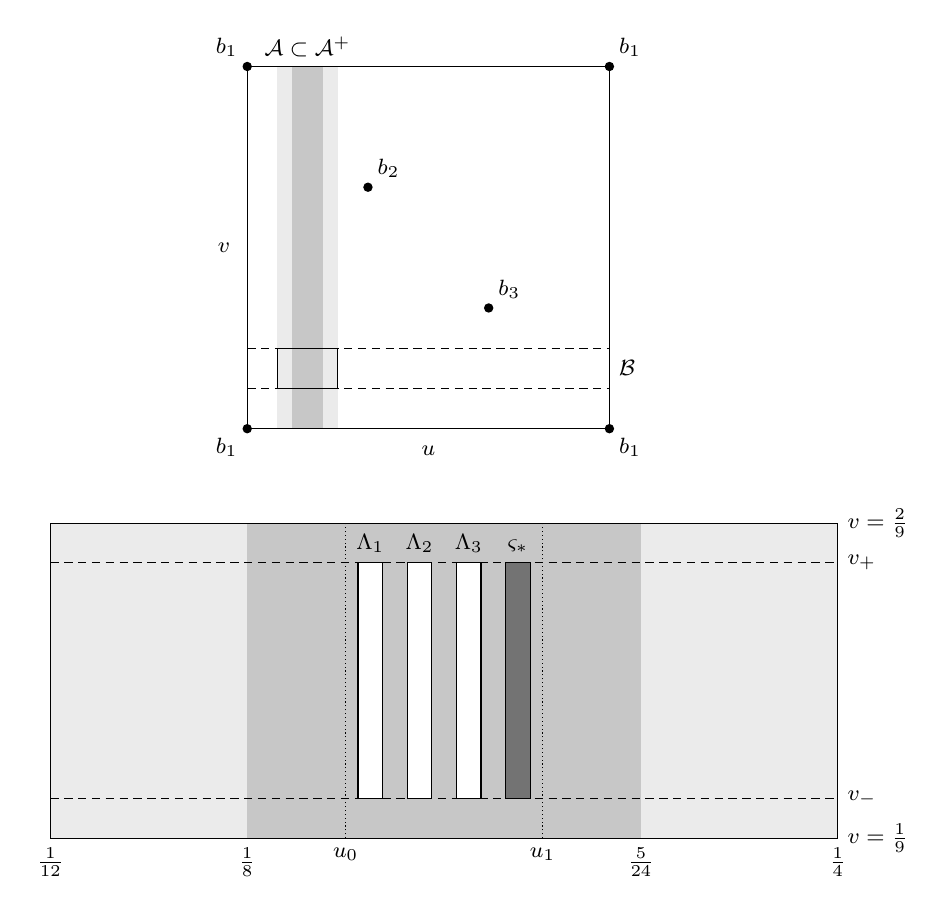
\begin{tikzpicture}[font=\footnotesize]
 \begin{scope}[scale=4.6]
  \fill[black!8] (1/12,0) rectangle (1/4,1);
  \fill[black!22] (1/8,0) rectangle (5/24,1);
  \draw[densely dashed] (0,1/9) -- (1,1/9);
  \draw[densely dashed] (0,2/9) -- (1,2/9);
  \draw (0,0) rectangle (1,1);
  \draw[thin] (1/12,1/9) rectangle (1/4,2/9);
  \foreach \p in {(0,0),(1,0),(0,1),(1,1),(1/3,2/3),(2/3,1/3)} \fill \p circle (0.013);
  \node[below left] at (0,0) {$b_1$};
  \node[below right] at (1,0) {$b_1$};
  \node[above left] at (0,1) {$b_1$};
  \node[above right] at (1,1) {$b_1$};
  \node[above right] at (1/3,2/3) {$b_2$};
  \node[above right] at (2/3,1/3) {$b_3$};
  \node[above] at (1/6,1) {$\mathcal A\subset\mathcal A^+$};
  \node[right] at (1,1/6) {$\mathcal B$};
  \node[below] at (1/2,-0.02) {$u$};
  \node[left] at (-0.02,1/2) {$v$};
 \end{scope}
 \begin{scope}[shift={(-2.5,-5.2)},x=60cm,y=36cm,shift={(-1/12,-1/9)}]
  \fill[black!8] (1/12,1/9) rectangle (1/4,2/9);
  \fill[black!22] (1/8,1/9) rectangle (5/24,2/9);
  \draw (1/12,1/9) rectangle (1/4,2/9);
  \draw[densely dashed] (1/12,1/8) -- (1/4,1/8);
  \draw[densely dashed] (1/12,5/24) -- (1/4,5/24);
  \filldraw[fill=white] (0.14844,1/8) rectangle (0.15365,5/24);
  \node[above] at (0.15104,5/24) {$\Lambda_1$};
  \filldraw[fill=white] (0.15885,1/8) rectangle (0.16406,5/24);
  \node[above] at (0.16146,5/24) {$\Lambda_2$};
  \filldraw[fill=white] (0.16927,1/8) rectangle (0.17448,5/24);
  \node[above] at (0.17188,5/24) {$\Lambda_3$};
  \filldraw[fill=black!55] (0.17969,1/8) rectangle (0.18490,5/24);
  \node[above] at (0.18229,5/24) {$\varsigma_*$};
  \draw[densely dotted] (7/48,1/9) -- (7/48,2/9);
  \draw[densely dotted] (3/16,1/9) -- (3/16,2/9);
  \node[below] at (7/48,1/9) {$u_0$};
  \node[below] at (3/16,1/9) {$u_1$};
  \node[below] at (1/8,1/9) {$\frac18$};
  \node[below] at (5/24,1/9) {$\frac5{24}$};
  \node[below] at (1/12,1/9) {$\frac1{12}$};
  \node[below] at (1/4,1/9) {$\frac14$};
  \node[right] at (1/4,1/8) {$v_-$};
  \node[right] at (1/4,5/24) {$v_+$};
  \node[right] at (1/4,1/9) {$v=\frac19$};
  \node[right] at (1/4,2/9) {$v=\frac29$};
 \end{scope}
\end{tikzpicture}
\caption{The handle data on the base torus $\Gamma=(\R/\Z)^2$ in the coordinates $(u,v)$ (Proposition~\ref{prop:cub-handle},
Definition~\ref{def:shd4-frame}). Top: the annuli $\mathcal A\subset\mathcal A^+$ (dark and light grey), the dual band
$\mathcal B$ (between the dashed lines $v=\frac19$, $v=\frac29$) and the marked points $b_1,b_2,b_3$, at which $Z_0=0$. Bottom: the rectangle
$\mathcal A^+\cap\mathcal B$ enlarged, with dashed lines at $v=v_\pm$; the clock $f$ rises on $[u_0,u_1]$, and the layers $\Lambda_i$ (white) and the
residual layer, where $\varsigma_*$ rises (black), lie over $(l_j,r_j)\times(v_-,v_+)$, where $b>0$. Drawn for $k=3$.}
\label{fig:shd4-handle}
\end{figure}

\begin{lemma}[The first path in the frame]\label{lem:shd4-frame-forms}
\lean{SymplecticPacking.Handle.Cubic.OmegaT_frameA, SymplecticPacking.Handle.Cubic.OmegaT_one_frameA,
SymplecticPacking.Handle.Cubic.Omega1Loc}
Over $\mathcal A^+$, $\chi_{\mathcal A}^*\Omega_t=\omega_V+\kappa_t+dp\wedge(a_{\mathcal A}+t\,\partial_p\alpha_1)$ with the positive forms
$\kappa_t$ of Lemma~\ref{lem:fer-positivity}. Over $\mathcal A$,
\[
 \chi_{\mathcal A}^*\Omega_1=\omega_V+e_h\nu+d\bigl(f(u)H^*(p)\beta\bigr).
\]
\end{lemma}

\begin{proof}
The first identity is Lemma~\ref{lem:fer-positivity}, written in the frame of Lemma~\ref{lem:fer-frame}. The second
is Lemma~\ref{lem:fer-alpha1}(ii), with $d\Gamma_{\rm sm}=e_h\nu$.
\end{proof}

\emph{The twist.} For $\lambda\in\R$ define on $\mathcal A\times\C$
\begin{equation}\label{eq:shd4-twist}
\begin{gathered}
 \mathcal D_\lambda(u,v,w_{\mathcal A})=\bigl(u,v,q_{\lambda f(u)}(w_{\mathcal A})\bigr),\qquad
 \mathcal D_\lambda^{-1}(u,v,w_{\mathcal A})=\bigl(u,v,q^{-1}_{\lambda f(u)}(w_{\mathcal A})\bigr),\\
 Q^\lambda_u=\lambda f'(u)\,Q_{\lambda f(u)},\qquad G_\lambda(u,w_{\mathcal A})=f(u)\,H^*\bigl(p(q_\lambda^{-1}w_{\mathcal A})\bigr),
\end{gathered}
\end{equation}
and $\mathcal D=\mathcal D_1$. These maps are smooth in $(\lambda,u,v,w_{\mathcal A})$ and mutually inverse, fix base points and
preserve $\mathcal A\times D(c)$ for every $c>P_{\rm supp}$.
\lean{SymplecticPacking.Handle.Cubic.Dlam, SymplecticPacking.Handle.Cubic.DlamInv, SymplecticPacking.Handle.Cubic.Qs,
SymplecticPacking.Handle.Cubic.Glam}

\begin{lemma}[Suspension]\label{lem:shd4-suspension}
\lean{SymplecticPacking.Handle.Cubic.suspension}
On $\mathcal A\times\C$, $\mathcal D_\lambda^*\omega_V=\omega_V+d\bigl[(Q^\lambda_u\circ q_{\lambda f(u)})\,du\bigr]$ for every $\lambda$.
\end{lemma}

\begin{proof}
This is \Mref{Lemma}{lem:hdl-suspension}(i) with $m=1$ and $s$ replaced by $u$: the differential of $\mathcal D_\lambda$ fixes
$\partial_v$, maps a vertical vector $\xi$ to $Dq\,\xi$ and $\partial_u$ to $\partial_u+X_{Q^\lambda_u}$, and $q_{\lambda f(u)}$ is symplectic.
\end{proof}

\emph{Periodisation.} For a one-form $\alpha$ on $\widetilde N$ supported over $\{u_0\le u\le u_1\}$ put
$\operatorname{per}(\alpha)=\sum_{m\in\Z}(T_u^m)^*\alpha$. The supports of the summands lie over the disjoint intervals
$[u_0-m,u_1-m]$, so the sum is locally finite; $\operatorname{per}(\alpha)$ is $T_u$-invariant, agrees with $\alpha$ over
$\{u_1-1<u<1+u_0\}$, and vanishes near every point whose $u$-coordinate is not in $[u_0,u_1]+\Z$. If $\alpha$ is horizontal, then
at a point with $\lfloor u\rfloor=m$ it is the covector of $\alpha$ at $T_u^{-m}$ of that point.
\lean{SymplecticPacking.Handle.Ush, SymplecticPacking.Handle.perJ}

\begin{construction}[The second-path primitive]\label{cons:shd4-eta}
\lean{SymplecticPacking.Handle.Cubic.etaLoc, SymplecticPacking.Handle.Cubic.eta, SymplecticPacking.Handle.Cubic.etaPer,
SymplecticPacking.Handle.Cubic.etaDot, SymplecticPacking.Handle.Cubic.OmS1}
On $\mathcal A\times\C$ let
\[
 \upsilon^{\mathcal A}_\lambda=\bigl(Q^\lambda_u\circ q_{\lambda f(u)}\bigr)\,du
 +f(u)\Bigl[H^*\bigl(p(q_\lambda^{-1}q_{\lambda f(u)}w_{\mathcal A})\bigr)-H^*\bigl(p(w_{\mathcal A})\bigr)\Bigr]\beta .
\]
Let $\upsilon_\lambda$ be the one-form on $\widetilde N$ equal to $(\chi_{\mathcal A}^{-1})^*\upsilon^{\mathcal A}_\lambda$ over $\mathcal A$ and to zero
elsewhere, let $\upsilon^{\rm per}_\lambda=\operatorname{per}(\upsilon_\lambda)$, and put
\[
 \Omega^{(1)}_\lambda=\Omega_1+d\upsilon^{\rm per}_\lambda,\qquad \dot\upsilon_\lambda=\partial_\lambda\upsilon^{\rm per}_\lambda .
\]
\end{construction}

\begin{lemma}[Properties of the second-path primitive]\label{lem:shd4-eta}
\lean{SymplecticPacking.Handle.Cubic.etaLoc_eq_zero_of_s, SymplecticPacking.Handle.Cubic.etaLoc_eq_zero_of_p,
SymplecticPacking.Handle.Cubic.eta_support, SymplecticPacking.Handle.Cubic.eta_smooth, SymplecticPacking.Handle.Cubic.eta_zero,
SymplecticPacking.Handle.Cubic.eta_horizontal, SymplecticPacking.Handle.Cubic.eta_TvE, SymplecticPacking.Handle.Cubic.etaDot_far,
SymplecticPacking.Handle.Cubic.firstStage_eq_pre}
\begin{enumerate}[label=(\alph*)]
\item $\upsilon^{\mathcal A}_\lambda$ vanishes for $u\le u_0$, for $u\ge u_1$, and for $p>P_{\rm supp}$; $\upsilon^{\mathcal A}_0=0$.
\item $\upsilon_\lambda$ and $\upsilon^{\rm per}_\lambda$ are horizontal one-forms on $\widetilde N$, smooth in $(\lambda,x)$; $\upsilon_\lambda$ is
$T_v$-invariant, $\upsilon^{\rm per}_\lambda$ is invariant under all deck maps, and $\upsilon^{\rm per}_0=0$. Both $\upsilon^{\rm per}_\lambda$ and $\dot\upsilon_\lambda$ vanish near every point with $p>P_{\rm supp}$ or with
$u\notin[u_0,u_1]+\Z$.
\item Over $\mathcal A$,
$\chi_{\mathcal A}^*\Omega^{(1)}_\lambda=\mathcal D_\lambda^*\bigl(\omega_V+e_h\nu+d(G_\lambda\beta)\bigr)$.
\end{enumerate}
\end{lemma}

\begin{proof}
(a) For $u\le u_0$, $f=f'=0$. For $u\ge u_1$, $f'=0$ and $q_\lambda^{-1}q_{\lambda f(u)}=q_\lambda^{-1}q_\lambda=\mathrm{id}$, so the bracket vanishes.
For $p>P_{\rm supp}$, $Q_t=0$ near $w_{\mathcal A}$ and all $q_t$, $q_t^{-1}$ fix $w_{\mathcal A}$. At $\lambda=0$ both terms vanish.

(b) By (a), $\upsilon^{\mathcal A}_\lambda$ vanishes over collars of both ends of $\mathcal A$, so the extension by zero is smooth. The form
$\upsilon^{\mathcal A}_\lambda$ has only $du$ and $dv$ components, and $\chi_{\mathcal A}$ preserves base points, so $\upsilon_\lambda$ is horizontal.
The coefficients of $\upsilon^{\mathcal A}_\lambda$ are $1$-periodic in $v$, since $b$ is periodic and $\mathcal D_\lambda$, $G_\lambda$ do not
depend on $v$; with $\chi_{\mathcal A}(u,v+1,\cdot)=T_v\chi_{\mathcal A}(u,v,\cdot)$ this gives $T_v^*\upsilon_\lambda=\upsilon_\lambda$. The
periodisation is $T_u$-invariant, and $T_v$-invariant because $T_u$ and $T_v$ commute. The support statement follows from (a)
and the properties of $\operatorname{per}$, and it passes to the $\lambda$-derivative.

(c) Over $\mathcal A$ the form $\upsilon^{\rm per}_\lambda$ is $\upsilon_\lambda$. The map $\mathcal D_\lambda$ fixes base points, so it preserves $\nu$ and
$\beta$ and $\mathcal D_\lambda^*(G_\lambda\beta)=(G_\lambda\circ\mathcal D_\lambda)\beta$ with
$G_\lambda\circ\mathcal D_\lambda=f(u)H^*(p(q_\lambda^{-1}q_{\lambda f(u)}w_{\mathcal A}))$. Add
Lemma~\ref{lem:shd4-suspension} to Lemma~\ref{lem:shd4-frame-forms}.
\end{proof}

\begin{proposition}[The second path]\label{prop:shd4-second}
\lean{SymplecticPacking.Handle.Cubic.OmegaPreG_split, SymplecticPacking.Handle.Cubic.firstStage_nondeg,
SymplecticPacking.Handle.Cubic.OmS1_preserves, SymplecticPacking.Handle.Cubic.twist_bound,
SymplecticPacking.Handle.Cubic.Hstar_twist_nonneg}
For valid cubic data and $\lambda\in[0,1]$, the form $\Omega^{(1)}_\lambda$ is closed, invariant under all deck maps, equal to
$\Omega_1$ for $\lambda=0$, and nondegenerate at every point of $\{p<h+2\delta_m\}$.
\end{proposition}

\begin{proof}
Closedness, invariance and $\Omega^{(1)}_0=\Omega_1$ follow from Lemma~\ref{lem:shd4-eta}(b) and the invariance of
$\Omega_1$ (Lemma~\ref{lem:fer-positivity}). Since deck maps preserve $p$ and the form, it suffices to check
nondegeneracy over $\{u_1-1<u<1+u_0\}$. Near points with $u\notin[u_0,u_1]$ the form is $\Omega_1$, which is symplectic
on $\{p<\frac13-e_h/9\}\supset\{p<h+2\delta_m\}$ (Lemmas~\ref{lem:fer-positivity} and~\ref{lem:shd4-budget}(d)). Over
$\mathcal A$ use Lemma~\ref{lem:shd4-eta}(c). By \Mref{Lemma}{lem:hdl-top-power}(b) with $n=2$, $\sigma_\Sigma=\nu$ and $e=e_h$,
\[
 \bigl(\omega_V+e_h\nu+d(G_\lambda\beta)\bigr)^2=2\bigl(e_h+b(v)\,\partial_uG_\lambda\bigr)\,\omega_V\wedge\nu,\qquad
 \partial_uG_\lambda(u,w')=f'(u)\,H^*\bigl(p(q_\lambda^{-1}w')\bigr).
\]
If $p(w_{\mathcal A})<h+2\delta_m$, then $w'=q_{\lambda f(u)}(w_{\mathcal A})$ and $q_\lambda^{-1}w'$ lie in $D(h+2\delta_m)$, because
$h+2\delta_m>P_{\rm supp}$; Lemma~\ref{lem:shd4-budget}(d) gives $H^*>0$ there. Since $f'\ge0$, $b\ge0$ and $e_h>0$, the
coefficient is positive at $\mathcal D_\lambda(x)$, and $\mathcal D_\lambda$ and $\chi_{\mathcal A}$ are diffeomorphisms.
\end{proof}

\emph{The final coefficient.} With the residual of Definition~\ref{def:shd4-scalars} put
\[
 G_{\rm f}(u,w)=J\bigl(p(w)\bigr)+\sum_{i=1}^k\varsigma_i(u)\,h_i\bigl(p(w)\bigr)+\varsigma_*(u)\,R^*(w),\qquad
 A_i=J+\sum_{j<i}h_j .
\]
\lean{SymplecticPacking.Handle.Cubic.Gf, SymplecticPacking.Handle.Cubic.aLayer}

\begin{lemma}[The final coefficient]\label{lem:shd4-Gf}
\lean{SymplecticPacking.Handle.Cubic.contDiff_Gf, SymplecticPacking.Handle.Cubic.Gf_mono, SymplecticPacking.Handle.Cubic.Gf_low,
SymplecticPacking.Handle.Cubic.Gf_up, SymplecticPacking.Handle.Cubic.Gf_layer}
For valid cubic data, $G_{\rm f}$ is smooth on $\R\times\C$ and
\begin{enumerate}[label=(\alph*)]
\item $\partial_uG_{\rm f}=\sum_i\varsigma_i'h_i\circ p+\varsigma_*'R^*\ge0$ at every $(u,w)$ with $R^*(w)\ge0$;
\item $G_{\rm f}=J\circ p$ for $u\le l_1$, and $G_{\rm f}=K\circ p\circ q^{-1}$ for $u\ge r_*$;
\item $G_{\rm f}(u,w)=A_i(p(w))+\varsigma_i(u)h_i(p(w))$ for $l_i<u<r_i$, $1\le i\le k$.
\end{enumerate}
\end{lemma}

\begin{proof}
(a) Differentiate; $h_i>0$ by Lemma~\ref{lem:shd4-budget}(a), and $\varsigma_j'\ge0$. (b) For $u\le l_1$ all clocks vanish. For
$u\ge r_*$ all equal one, and $J+\sum_ih_i+R^*=K\circ p\circ q^{-1}$. (c) On $(l_i,r_i)$, $\varsigma_j=1$ for $j<i$ and $\varsigma_j=0$ for
$j>i$, including $j=*$.
\end{proof}

\begin{construction}[The third-path primitive]\label{cons:shd4-xi}
\lean{SymplecticPacking.Handle.Cubic.Gdiff, SymplecticPacking.Handle.Cubic.xiA, SymplecticPacking.Handle.Cubic.JbE,
SymplecticPacking.Handle.Cubic.xi, SymplecticPacking.Handle.Cubic.xiPer, SymplecticPacking.Handle.Cubic.OmS2,
SymplecticPacking.Handle.Cubic.OmegaFinalPer, SymplecticPacking.Handle.Cubic.Ghat}
On $\mathcal A\times\C$ let $\xi^{\mathcal A}=\bigl((G_{\rm f}-G_1)\circ\mathcal D\bigr)\beta$. Let $\xi$ be the one-form on $\widetilde N$ equal to
$J(p)\beta+(\chi_{\mathcal A}^{-1})^*\bigl(\xi^{\mathcal A}-J(p)\beta\bigr)$ over $\mathcal A$ and to $J(p)\beta$ elsewhere, and put
\[
\begin{gathered}
 \xi^{\rm per}=J(p)\beta+\operatorname{per}\bigl(\xi-J(p)\beta\bigr),\qquad
 \Omega^{(2)}_\tau=\Omega^{(1)}_1+\tau\,d\xi^{\rm per},\\
 \Omega_{\rm fin}=\Omega^{(2)}_1,\qquad \hat G_\tau=(1-\tau)G_1+\tau G_{\rm f}.
\end{gathered}
\]
\end{construction}

\begin{lemma}[Properties of the third-path primitive]\label{lem:shd4-xi}
\lean{SymplecticPacking.Handle.Cubic.xi_collar, SymplecticPacking.Handle.Cubic.xi_smooth,
SymplecticPacking.Handle.Cubic.xi_horizontal, SymplecticPacking.Handle.Cubic.xi_toric_near_boundary,
SymplecticPacking.Handle.Cubic.xi_TvE, SymplecticPacking.Handle.Cubic.xiPer_deck, SymplecticPacking.Handle.Cubic.xiPer_eq_fX,
SymplecticPacking.Handle.Cubic.fX_far, SymplecticPacking.Handle.Cubic.secondStage_eq_on_A,
SymplecticPacking.Handle.Cubic.secondStage_off}
\begin{enumerate}[label=(\alph*)]
\item $\xi^{\mathcal A}=J(p)\beta$ for $u\le u_0$ and for $u\ge u_1$.
\item $\xi^{\rm per}$ is a smooth one-form on $\widetilde N$, invariant under all deck maps, of the form $\Xi\,\beta$ with $\Xi$ smooth; on
$\{p>P_{\rm supp}\}$, $\Xi$ is a function of $(u\bmod1,p)$.
\item Over $\mathcal A$, $\chi_{\mathcal A}^*\Omega^{(2)}_\tau=\mathcal D^*\bigl(\omega_V+e_h\nu+d(\hat G_\tau\beta)\bigr)$; near points with
$u\notin[u_0,u_1]+\Z$, $\Omega^{(2)}_\tau=\Omega_1+\tau J'(p)\,b(v)\,dp\wedge dv$.
\end{enumerate}
\end{lemma}

\begin{proof}
(a) For $u\le u_0$, $\mathcal D=\mathrm{id}$, $G_1=0$ and $G_{\rm f}=J\circ p$, since $u_0<l_1$. For $u\ge u_1>r_*$,
$G_1\circ\mathcal D=H^*(p(q^{-1}qw_{\mathcal A}))=H^*(p)$ and $G_{\rm f}\circ\mathcal D=K(p(q^{-1}qw_{\mathcal A}))=K(p)$, whose difference is $J(p)$.

(b) By (a), $\xi-J(p)\beta$ vanishes over collars of both ends of $\mathcal A$ and is supported over $[u_0,u_1]$, so $\xi$ and
the periodisation are smooth. Both summands are multiples of $\beta$: $\chi_{\mathcal A}$ preserves base points. Invariance
follows as in Lemma~\ref{lem:shd4-eta}(b), and $J(p)\beta$ is invariant because deck maps preserve $p$ and $v\bmod1$. On
$\{p>P_{\rm supp}\}$ all $q_t$ are the identity, $\mathcal D=\mathrm{id}$, and $G_1$, $G_{\rm f}$ are functions of $(u,p)$.

(c) Over $\mathcal A$, $\xi^{\rm per}=\xi$ and $\chi_{\mathcal A}^*\xi=\xi^{\mathcal A}=\mathcal D^*((G_{\rm f}-G_1)\beta)$; add
Lemma~\ref{lem:shd4-eta}(c) at $\lambda=1$. Near points with $u\notin[u_0,u_1]+\Z$, $\upsilon^{\rm per}_1=0$ and $\xi^{\rm per}=J(p)\beta$, and
$d(J(p)\beta)=J'(p)b(v)\,dp\wedge dv$.
\end{proof}

\begin{proposition}[The third path and the final form]\label{prop:shd4-third}
\lean{SymplecticPacking.Handle.Cubic.secondStage_nondeg, SymplecticPacking.Handle.Cubic.OmS2_preserves,
SymplecticPacking.Handle.Cubic.OmegaFinalPer_eq, SymplecticPacking.Handle.Cubic.OmegaFinal_eq_pullback,
SymplecticPacking.Strip.Cubic.DinvN, SymplecticPacking.Strip.Cubic.DinvN_pullback}
For valid cubic data and $\tau\in[0,1]$, $\Omega^{(2)}_\tau$ is closed, invariant under all deck maps and nondegenerate at every
point of $\{p<h+2\delta_m\}$. Over $\mathcal A$,
\[
 \chi_{\mathcal A}^*\Omega_{\rm fin}=\mathcal D^*\Omega_{\rm pre},\qquad
 (\chi_{\mathcal A}\circ\mathcal D^{-1})^*\Omega_{\rm fin}=\Omega_{\rm pre},\qquad
 \Omega_{\rm pre}=\omega_V+e_h\nu+d(G_{\rm f}\beta),
\]
and $\chi_{\mathcal A}\circ\mathcal D^{-1}$ maps $\mathcal A\times D(h)$ diffeomorphically onto $\mathcal A\times D(h)$.
\end{proposition}

\begin{proof}
Closedness and invariance follow from Proposition~\ref{prop:shd4-second} and Lemma~\ref{lem:shd4-xi}(b). As before it
suffices to work over $\{u_1-1<u<1+u_0\}$. Over $\mathcal A$, by Lemma~\ref{lem:shd4-xi}(c) and
\Mref{Lemma}{lem:hdl-top-power}(b), the square is $2(e_h+b\,\partial_u\hat G_\tau)\,\omega_V\wedge\nu$ at the image point
$\mathcal D(x)$, and $\partial_u\hat G_\tau=(1-\tau)\partial_uG_1+\tau\partial_uG_{\rm f}$. For $p(x)<h+2\delta_m$ the image fibre point $w'$ has
$p(w')<h+2\delta_m$; $\partial_uG_1(u,w')\ge0$ as in Proposition~\ref{prop:shd4-second}, and $\partial_uG_{\rm f}(u,w')\ge0$ by
Lemmas~\ref{lem:shd4-Gf}(a) and~\ref{lem:shd4-budget}(d). Near points with $u\notin[u_0,u_1]$, Lemma~\ref{lem:shd4-xi}(c) adds to
$\Omega_1$ a term $dp\wedge(\cdot)$ with a base one-form; in the local form of Lemma~\ref{lem:fer-positivity} it only changes the
mixed part, so the square is still $2\omega_V\wedge\kappa_1>0$ (Lemma~\ref{lem:pre-top-power}). The displayed identities are
Lemma~\ref{lem:shd4-xi}(c) at $\tau=1$. The last statement holds because $\mathcal D^{\pm1}$ fix base points and $q_t^{\pm1}$ preserve
$D(h)$, while $\chi_{\mathcal A}$ preserves $p$.
\end{proof}

\begin{lemma}[Vanishing on the marked fibres]\label{lem:shd4-fibres}
\lean{SymplecticPacking.Handle.fibreSetH, SymplecticPacking.Handle.Cubic.alpha1E_fibre,
SymplecticPacking.Handle.Cubic.etaDot_fibre, SymplecticPacking.Handle.Cubic.xiPer_fibre,
SymplecticPacking.Handle.Cubic.xi_zero_of_bB, SymplecticPacking.Handle.Cubic.xiPer_fibre}
Let $\widetilde{\mathcal F}$ be the union of all lifts of the fibres $N_{b_1},N_{b_2},N_{b_3}$, that is, the set of points
$(u,v,w)$ with $(u,v)\in b_j+\Z^2$ for some $j$. At every point of $\widetilde{\mathcal F}$ the covectors $\alpha_1$, $\dot\upsilon_\lambda$ $(\lambda\in\R)$ and $\xi^{\rm per}$ of
$T^*\widetilde N$ are zero.
\end{lemma}

\begin{proof}
For $\alpha_1$ this is Lemma~\ref{lem:fer-alpha1-fibres}, lifted to the cover, where $\alpha_1$ is periodic. The
$u$-coordinates of the $b_j$ are $0,\frac13,\frac23$, which are not in $[u_0,u_1]=[\frac7{48},\frac9{48}]$ modulo one, so
$\dot\upsilon_\lambda$ vanishes near $\widetilde{\mathcal F}$ by Lemma~\ref{lem:shd4-eta}(b). By Lemma~\ref{lem:shd4-xi}(b),
$\xi^{\rm per}=\Xi\,b(v)\,dv$; the $v$-coordinates of the $b_j$ are $0,\frac23,\frac13$, and $b$ vanishes outside
$[\frac18,\frac5{24}]+\Z$ (Proposition~\ref{prop:cub-handle}(c)), so $\beta$ vanishes at every point of
$\widetilde{\mathcal F}$.
\end{proof}

\begin{construction}[The handle Moser map]\label{cons:shd4-moser}
\lean{SymplecticPacking.Handle.Cubic.stage0, SymplecticPacking.Handle.Cubic.stage1, SymplecticPacking.Handle.Cubic.stage2,
SymplecticPacking.Handle.clock, SymplecticPacking.Handle.moserPathB, SymplecticPacking.Handle.moserVariationB,
SymplecticPacking.Handle.concat3B, SymplecticPacking.Handle.Cubic.handleData, SymplecticPacking.Handle.Cubic.handleParams,
SymplecticPacking.Handle.solve4, SymplecticPacking.Handle.cutoffChi, SymplecticPacking.Handle.boxFieldP,
SymplecticPacking.Handle.Cubic.handlePhi, SymplecticPacking.Handle.Cubic.handlePhiInv}
The three stages are
\[
 (\Omega^{(0)}_s,\mathfrak v^{(0)}_s)=(\Omega_s,\alpha_1),\qquad
 (\Omega^{(1)}_s,\mathfrak v^{(1)}_s)=(\Omega^{(1)}_s,\dot\upsilon_s),\qquad
 (\Omega^{(2)}_s,\mathfrak v^{(2)}_s)=(\Omega^{(2)}_s,\xi^{\rm per}),
\]
with matching endpoints $\Omega^{(0)}_1=\Omega^{(1)}_0$ and $\Omega^{(1)}_1=\Omega^{(2)}_0$. With the clocks $\sigma_i(t)=S(9t-3i-1)$,
$i=0,1,2$, which move only on $[\frac{3i+1}9,\frac{3i+2}9]$, put
\[
 \Omega^{\rm M}_t=\Omega^{(0)}_{\sigma_0(t)}+\sum_{i=1,2}\bigl(\Omega^{(i)}_{\sigma_i(t)}-\Omega^{(i)}_0\bigr),\qquad
 \mathfrak v_t=\sum_{i=0}^2\sigma_i'(t)\,\mathfrak v^{(i)}_{\sigma_i(t)} .
\]
On $U=\{p<h+2\delta_m\}$ let $Y_t$ be the field with $\iota_{Y_t}\Omega^{\rm M}_t=-\mathfrak v_t$; in the coordinates
$(\operatorname{Re}w,\operatorname{Im}w,u,v)$ it is the adjugate solution of a $4\times4$ skew system. With the moment cutoff
\[
 \mathfrak c(p)=S\Bigl(\frac{h+\frac74\delta_m-p}{\delta_m/4}\Bigr),
\]
which equals one for $p\le h+\frac32\delta_m$ and zero for $p\ge h+\frac74\delta_m$, let $\widehat Y_t=\mathfrak c(p)Y_t$, extended by zero.
The handle Moser map $\Phi$ is the time-one map of $\widehat Y$ from time $0$, and $\Phi^{-1}$ is its inverse.
\end{construction}

The bordered construction of \Msec{sec:hdl} cuts each path off by a whole-path Gram cutoff of a finite atlas,
because nondegeneracy is known only near the compact model region. Here the cover has one global chart and every stage
form is nondegenerate on the whole set $U$ for parameters in $[0,1]$; the moment cutoff $\mathfrak c(p)$ is the only cutoff, and
completeness comes from deck invariance.

\begin{proposition}[The handle Moser map]\label{prop:shd4-moser}
\lean[needed]{SymplecticPacking.Handle.Cubic.handleMoser, SymplecticPacking.Handle.handle_moser_global,
SymplecticPacking.Handle.Cubic.OmegaT_toric, SymplecticPacking.Handle.Cubic.etaDot_far,
SymplecticPacking.Handle.Cubic.d1_xiPer_toric, SymplecticPacking.Handle.Cubic.handleData_pres}
For valid cubic data, $\Phi$ and $\Phi^{-1}$ are mutually inverse $C^\infty$ diffeomorphisms of $\widetilde N$, and:
\begin{enumerate}[label=(\alph*)]
\item $\Phi^*\Omega_{\rm fin}=\Omega_0$ and $(\Phi^{-1})^*\Omega_0=\Omega_{\rm fin}$ at every point of $\{p\le h+\delta_m\}$;
\item for every $c>P_{\rm supp}$, $\Phi$ and $\Phi^{-1}$ map each of $\{p\le c\}$, $\{p<c\}$, $\{p=c\}$ onto itself;
\item $\Phi$ and $\Phi^{-1}$ fix every point of $\widetilde{\mathcal F}$;
\item $\Phi$ and $\Phi^{-1}$ commute with every deck map.
\end{enumerate}
Moreover $\Phi=\Phi_2\circ\Phi_1\circ\Phi_0$, where $\Phi_i$ is the time-one map of the cut stage field $\mathfrak c(p)Y^{(i)}_s$,
$\iota_{Y^{(i)}_s}\Omega^{(i)}_s=-\mathfrak v^{(i)}_s$.
\end{proposition}

\begin{proof}
\emph{Hypotheses.} On $[\frac{3i+1}9,\frac{3i+2}9]$ only $\sigma_i$ moves, so by the matching endpoints $\Omega^{\rm M}_t=\Omega^{(i)}_{\sigma_i(t)}$
there, and $\Omega^{\rm M}_t$ is $\Omega_0$ for $t\le\frac19$ and $\Omega_{\rm fin}$ for $t\ge\frac89$. Hence $\Omega^{\rm M}_t$ is closed and
nondegenerate on $U$ for every $t$ (Lemma~\ref{lem:fer-positivity} with Lemma~\ref{lem:shd4-budget}(d), and
Propositions~\ref{prop:shd4-second}, \ref{prop:shd4-third}). The pair is smooth on $\R\times\widetilde N$, and $\partial_t\Omega^{\rm M}_t=d\mathfrak v_t$ because
$\partial_s\Omega^{(i)}_s=d\mathfrak v^{(i)}_s$ for each stage; $\mathfrak v_t=0$ for $t\notin(0,1)$. By
Lemma~\ref{lem:pre-moser}(a), $Y$ is smooth on $\R\times U$, so $\widehat Y$ is smooth on $\R\times\widetilde N$. All stage forms and
primitives are deck invariant, and so is $\mathfrak c(p)$, since the deck maps preserve $p$.

\emph{Toric band.} Let $R=2\pi(-y\partial_x+x\partial_y)$, $w=x+iy$, generate the fibre rotation, so that $\iota_R\Omega_0=-dp$
(Lemma~\ref{lem:fer-positivity}). On $U'=\{P_{\rm supp}<p<h+2\delta_m\}$ one has $\iota_R\Omega^{\rm M}_t=-dp$ and $\mathfrak v_t(R)=0$:
$\alpha_1$ is horizontal and $\iota_Rd\alpha_1=0$; $\upsilon^{\rm per}_s$ and $\dot\upsilon_s$ vanish near $U'$
(Lemma~\ref{lem:shd4-eta}(b)); and on $U'$, $\xi^{\rm per}=\Xi(u\bmod1,p)\,b(v)\,dv$, whose differential has no fibre-angle
component, so $\iota_Rd\xi^{\rm per}=0=\xi^{\rm per}(R)$. Lemma~\ref{lem:pre-moser}(d) gives $dp(\widehat Y_t)=0$ on $\{p>P_{\rm supp}\}$, where
$\widehat Y$ vanishes for $p\ge h+\frac74\delta_m$.

\emph{Completeness.} The functions $du(\widehat Y_t)$, $dv(\widehat Y_t)$ are deck invariant (Lemma~\ref{lem:pre-moser}(g), since the
stage data and $\mathfrak c(p)$ are deck invariant), and deck maps
act on $(u,v)$ by integral translations; hence $|du(\widehat Y_t)|+|dv(\widehat Y_t)|\le C_b$, the maximum over the compact set
$[0,1]\times[0,1]^2\times\bar D(h+\frac74\delta_m)$, and $\widehat Y_t=0$ for $t\notin[0,1]$. By the toric band, an integral curve
through $x$ stays in $\{p\le\max(p(x),h)\}$, and its base coordinates move by at most $C_b$ in unit time. Integral curves
therefore remain in compact sets, and the flow and its inverse are defined on $\R\times\widetilde N$ and smooth.

\emph{Conclusions.} (b) follows from $dp(\widehat Y_t)=0$ on $\{p>P_{\rm supp}\}$, in both time directions. (a) For
$p(x)\le h+\delta_m$ the integral curve stays in $\{p\le h+\delta_m\}$, because $dp(\widehat Y_t)=0$ on $\{p>P_{\rm supp}\}$ (toric band)
and $P_{\rm supp}<h$. For the same reason the open set $\{p<h+\frac32\delta_m\}$ is invariant under the flow of $\widehat Y$, and
$\mathfrak c=1$ there, so $\widehat Y=Y$ on it and $\Phi$ agrees with the time-one map of the uncut field $Y$ on a neighbourhood of $x$.
Lemma~\ref{lem:pre-moser}(b) gives $(\Phi^*\Omega^{\rm M}_1)_x=(\Omega^{\rm M}_0)_x$. The inverse identity follows because
$\Phi^{-1}$ preserves $\{p\le h+\delta_m\}$. (c) By Lemma~\ref{lem:shd4-fibres}, $\mathfrak v_t=0$ on $\widetilde{\mathcal F}$ for every $t$,
so $\widehat Y_t=0$ there, and Lemma~\ref{lem:pre-moser}(c) applies in both time directions. (d) is
Lemma~\ref{lem:pre-moser}(g), since all stage forms and primitives and $\mathfrak c(p)$ are deck invariant.

\emph{Decomposition.} Each stage pair $(\Omega^{(i)}_s,\mathfrak v^{(i)}_s)$ is deck invariant and satisfies the same
rotation identity $\iota_R\Omega^{(i)}_s=-dp$, $\mathfrak v^{(i)}_s(R)=0$ on $U'$, so the completeness argument above applies
to each cut stage field $\mathfrak c(p)Y^{(i)}_s$; write $\Phi^{(i)}_s$ for its flow from time $0$ and $\Phi_i=\Phi^{(i)}_1$. On
$[\frac{3i+1}9,\frac{3i+2}9]$ the cut field is $\widehat Y_t=\sigma_i'(t)\mathfrak c(p)Y^{(i)}_{\sigma_i(t)}$, so
$t\mapsto\Phi^{(i)}_{\sigma_i(t)}(x)$ is an integral curve of $\widehat Y$ on that interval; on the gaps between these
intervals and for $t\notin[\frac19,\frac89]$ one has $\mathfrak v_t=0$, hence $\widehat Y_t=0$. By uniqueness of integral
curves, the integral curve of $\widehat Y$ through $x$ is obtained by running $\Phi^{(0)}$, $\Phi^{(1)}$, $\Phi^{(2)}$ in turn,
which gives $\Phi=\Phi_2\circ\Phi_1\circ\Phi_0$ (Lemma~\ref{lem:pre-moser}(f)).
\end{proof}

Equivalently, $\Phi$ is defined through compactly supported fields: for $A\ge0$ multiply $\widehat Y$ by a product
cutoff in $(u,v)$ equal to one on $\{|u|,|v|\le A+C_b+2\}$, let $\Phi_A$ be the time-one map of the cut field, and set $\Phi(x)=\Phi_A(x)$ with $A=|u(x)|+|v(x)|$. The base
speed bound shows that the integral curve through $x$ never meets the region where the box cutoff differs from one, so
this is the time-one map above.
\lean{SymplecticPacking.Handle.boxCut, SymplecticPacking.Handle.Cb, SymplecticPacking.Handle.boxL,
SymplecticPacking.Handle.PhiB, SymplecticPacking.Handle.PhiG, SymplecticPacking.Handle.PhiGInv,
SymplecticPacking.Handle.lfield_boxField, SymplecticPacking.Handle.LField.flowFrom_isSol, SymplecticPacking.Handle.flowFrom_box_eq}

\emph{Layer maps.} On the layer $\Lambda_i=\{l_i<u<r_i,\ \frac18<v<\frac5{24},\ p<h\}$ (frame coordinates) let
$T(v)=\int_{1/8}^vb$, a diffeomorphism of $(\frac18,\frac5{24})$ onto $(0,1)$ with $dT=\beta$ and inverse $v(T)$, and
\[
 \ell(T)=\frac{e_h}{b(v(T))},\qquad x_i(u,T,p)=(u-l_i)\,\ell(T)+\varsigma_i(u)\,h_i(p).
\]
Then $\partial_ux_i=\ell+\varsigma_i'h_i>0$, $x_i=0$ at $u=l_i$ and $x_i>h_i(p)$ at $u=r_i$, so for $0<x<h_i(p)$ and $0<T<1$ there is
a unique root $u=\sigma_i(x,T,p)\in(l_i,r_i)$. For $1\le i\le k$ put $\bar\rho_i=(\rho_i+a_i)/2$, $\delta_i=a_i-\bar\rho_i$,
$\hat\rho_i=\bar\rho_i+\delta_i/4$, and for $(z_{\rm b},z_{\rm f})\in\Bo(\hat\rho_i)\subset\C^2$ with $(x,T)=\Psi_{\delta_i}(z_{\rm b})$
(Proposition~\ref{prop:hdl-strip}) and $p=\pi|z_{\rm f}|^2$,
\[
 E_i(z_{\rm b},z_{\rm f})=\Bigl(\sigma_i(x,T,p),\ v(T),\ e^{-2\pi iTA_i'(p)}z_{\rm f}\Bigr),\qquad
 f^N_i=\Phi^{-1}\circ\chi_{\mathcal A}\circ\mathcal D^{-1}\circ E_i .
\]
\lean{SymplecticPacking.Strip.Cubic.ell, SymplecticPacking.Strip.Cubic.layerX, SymplecticPacking.Strip.Cubic.layerRoot,
SymplecticPacking.Strip.Cubic.shear, SymplecticPacking.Strip.Cubic.srcMap, SymplecticPacking.Strip.Cubic.layerMap,
SymplecticPacking.Strip.Cubic.layerMap_eq, SymplecticPacking.Strip.Cubic.fN}

\begin{proposition}[The four-dimensional embeddings into the cover]\label{prop:shd4-maps}
\lean[needed]{SymplecticPacking.Strip.Cubic.x_lt_hi, SymplecticPacking.Strip.Cubic.layer_form,
SymplecticPacking.Strip.Cubic.shear_pullback, SymplecticPacking.Strip.Cubic.layerMap_symplectic,
SymplecticPacking.Strip.Cubic.layerMap_mem_annulus, SymplecticPacking.Strip.Cubic.layerMap_injective,
SymplecticPacking.Strip.Cubic.layerMap_disjoint, SymplecticPacking.Strip.Cubic.layerMap_compact,
SymplecticPacking.Strip.Cubic.fN_mem, SymplecticPacking.Strip.Cubic.fN_smooth, SymplecticPacking.Strip.Cubic.fN_symplectic,
SymplecticPacking.Strip.Cubic.fN_eq_imp, SymplecticPacking.Strip.Cubic.fN_disjoint,
SymplecticPacking.Strip.Cubic.fN_avoid_fibres, SymplecticPacking.Strip.Cubic.fN_eq_imp,
SymplecticPacking.Embed.Cubic.fcap_eq_imp}
Let the cubic data be valid and $1\le i,j\le k$. Then $\rho_i<\bar\rho_i<\hat\rho_i<a_i$, and:
\begin{enumerate}[label=(\alph*)]
\item $f^N_i$ is defined and smooth on $\Bo(\hat\rho_i)$, with values in $\{p<h\}\setminus\widetilde{\mathcal F}$, and
$(f^N_i)^*\Omega_0=\omega_0$;
\item $f^N_i$ is injective, $f^N_i(\Bo(\hat\rho_i))\cap f^N_j(\Bo(\hat\rho_j))=\varnothing$ for $i\ne j$, and $f^N_i(B(\bar\rho_i))$ is compact;
\item if $f^N_i(X)=T\,f^N_j(X')$ for a deck map $T$, then $T=\mathrm{id}$, $i=j$ and $X=X'$.
\end{enumerate}
\end{proposition}

\begin{proof}
Let $\varpi=\pi|z_{\rm b}|^2$ and $\varpi+p<\hat\rho_i$. By Proposition~\ref{prop:hdl-strip} and Lemma~\ref{lem:shd4-budget}(a),
\[
 0<x<\varpi+\frac{\delta_i}2<\hat\rho_i-p+\frac{\delta_i}2=a_i-p-\frac{\delta_i}4<h_i(p),\qquad p<a_i<h,
\]
so the root exists, and $E_i$ maps $\Bo(\hat\rho_i)$ into $\Lambda_i$. Since $\ell\,b=e_h$, $e_h\nu=\ell\,du\wedge dT$; with
Lemma~\ref{lem:shd4-Gf}(c), $d(G_{\rm f}\beta)=(\varsigma_i'h_i\,du+dA_i+\varsigma_i\,dh_i)\wedge dT$ on $\Lambda_i$, hence
$\Omega_{\rm pre}=\omega_V+dx_i\wedge dT+dA_i(p)\wedge dT$ there. $E_i$ is the composite
of $\Psi_{\delta_i}\times\mathrm{id}$, the shear of Lemma~\ref{lem:hdl-shear} with $A=A_i$ and the inverse of the layer coordinates
$(u,v,w_{\mathcal A})\mapsto(x_i,T,w_{\mathcal A})$ (the periodic counterpart of the layer maps of Proposition~\ref{prop:str-layer}); by Proposition~\ref{prop:hdl-strip} and Lemma~\ref{lem:hdl-shear} it is a diffeomorphism onto an open subset of $\Lambda_i$ with $E_i^*\Omega_{\rm pre}=\omega_0$.

(a) By Proposition~\ref{prop:shd4-third}, $\chi_{\mathcal A}\mathcal D^{-1}$ maps $\Lambda_i$ into $\mathcal A\times D(h)$ and pulls $\Omega_{\rm fin}$ back
to $\Omega_{\rm pre}$; by Proposition~\ref{prop:shd4-moser}(a),(b), $\Phi^{-1}$ preserves $\{p<h\}$ and pulls $\Omega_0$ back to
$\Omega_{\rm fin}$ there. Composing gives $(f^N_i)^*\Omega_0=\omega_0$. The point $\chi_{\mathcal A}\mathcal D^{-1}E_i(X)$ lies over $\mathcal A$,
which misses $\widetilde{\mathcal F}$; if $\Phi^{-1}(y)\in\widetilde{\mathcal F}$, then $y=\Phi(\Phi^{-1}y)=\Phi^{-1}y\in\widetilde{\mathcal F}$ by
Proposition~\ref{prop:shd4-moser}(c).

(b) $E_i$ is injective, the images of different $E_i$ lie over the disjoint intervals $(l_i,r_i)$, and
$\chi_{\mathcal A}\mathcal D^{-1}$ and $\Phi^{-1}$ are injective maps common to all $i$. The closed ball is compact.

(c) By Proposition~\ref{prop:shd4-moser}(d), $\Phi^{-1}(y)=T\Phi^{-1}(y')=\Phi^{-1}(Ty')$ with $y=\chi_{\mathcal A}\mathcal D^{-1}E_i(X)$ and
$y'=\chi_{\mathcal A}\mathcal D^{-1}E_j(X')$, so $y=Ty'$. Both points lie over the square $(\frac18,\frac5{24})^2$, so the shift of $T$ is
zero and $T=\mathrm{id}$; then (b) gives $i=j$ and $X=X'$.
\end{proof}

\begin{remark}[The four-dimensional embeddings]\label{rem:shd-four}
\lean{SymplecticPacking.Embed.Cubic.fcap, SymplecticPacking.Embed.Cubic.fcapV, SymplecticPacking.Branch2.CubicData.fcapGen,
SymplecticPacking.Handle.Cubic.handleMoser, SymplecticPacking.Strip.fN, SymplecticPacking.Embed.Cubic.fcap,
SymplecticPacking.Branch2.embeddings2, SymplecticPacking.Branch2.embeddingsEq, SymplecticPacking.Branch2.CubicData.ofParams}
By Proposition~\ref{prop:shd4-maps}(a),(c) the maps $f^N_i$ satisfy the hypotheses of Theorem~\ref{thm:cub-transfer}, and
the four-dimensional embeddings are
$f^{\rm cap}_i=b_{\rm ball}\circ\mathcal T_{\rm u}\circ\mathsf N\circ f^N_i$ on $\Bo(\hat\rho_i)$. The general branch uses the data of Proposition~\ref{prop:scalar-cubic-data}
and the capacities of \eqref{eq:scalar-enlargement}. The equal branch uses the same maps for the data of
Remark~\ref{rem:rtc-equal}: $\rho_i=\rho$, $a_i=a$, $K(p)=(3\sqrt k-9)p$, and $(q_t)$ the isotopy of
Theorem~\ref{thm:pll-inner}, with the recorded capacities of Remark~\ref{rem:rtc-recorded}. The strip constants are
the four-dimensional values recorded in Definition~\ref{def:str-enlarged}: $\delta_i=a_i-\bar\rho_i=(a_i-\rho_i)/2$ and
$\hat\rho_i=a_i-\frac34\delta_i$; only the disc-to-strip map of Proposition~\ref{prop:str-strip} is taken from \S\ref{sec:str},
and the layer identities are proved in Proposition~\ref{prop:shd4-maps}.
\end{remark}

\subsection{The shear and the strip map}\label{sec:shd-shear}

The two explicit maps used in the layers of \Msec{sec:hdl-layers} are the following.

\begin{lemma}[Multi-angle shear]\label{lem:hdl-shear}
\lean{OAI.PackingSufficiencySupport.Hamiltonian.toricSuspension,
OAI.PackingSufficiencySupport.Hamiltonian.toricSuspensionInverse_smooth,
OAI.PackingSufficiencySupport.Hamiltonian.toricSuspension_pullback,
OAI.PackingSufficiencySupport.Hamiltonian.toricSuspensionInverse_left,
OAI.PackingSufficiencySupport.Hamiltonian.toricSuspensionInverse_right}
\uses{M-def:mech-model}
Let $A$ be a smooth function on an open set $W\subset\R^m$ and $\mathrm{Sh}_A(x,T,w)=(x,T,\mathrm{Sh}_{A,T}(w))$, where
\[
 \mathrm{Sh}_{A,T}(w)_j=\exp\big(-2\pi i\,T\,\partial_jA(p(w))\big)\,w_j\qquad(1\le j\le m),
\]
on $\{(x,T,w):p(w)\in W\}\subset\R^2\times\C^m$. Then $\mathrm{Sh}_A$ is a diffeomorphism of this set onto itself, preserves
$p$, $x$ and $T$, and
\[
 \mathrm{Sh}_A^*\big(\omega_V+dx\wedge dT+dA(p)\wedge dT\big)=\omega_V+dx\wedge dT .
\]
\end{lemma}

\begin{proof}
$\mathrm{Sh}_{A,T}$ multiplies each $w_j$ by a unimodular factor that is a smooth function of $(T,p(w))$; it preserves $p$, and the
same formula with $+2\pi i$ is its inverse. Both are smooth in Cartesian coordinates, also on the coordinate axes. Where all
$w_j\ne0$, write $w_j=\sqrt{p_j/\pi}\,e^{2\pi i\theta_j}$, so $\mathrm{Sh}_{A,T}$ is $\theta_j\mapsto\theta_j-T\partial_jA(p)$. Then
\[
 \mathrm{Sh}_A^*\omega_V=\sum_jdp_j\wedge d\big(\theta_j-T\partial_jA\big)
 =\omega_V-dA\wedge dT-T\sum_{j,k}\partial_{jk}A\,dp_j\wedge dp_k=\omega_V-dA\wedge dT,
\]
the Hessian term vanishing by symmetry; $dx\wedge dT$ and $dA(p)\wedge dT$ are unchanged since $x,T,p$ are. The identity extends
to the coordinate axes by continuity.
\end{proof}

\begin{proposition}[Disc-to-strip map]\label{prop:hdl-strip}
\lean{SymplecticPacking.Strip.psiStrip, SymplecticPacking.Strip.psiStrip_smooth,
 SymplecticPacking.Strip.psiStrip_symplectic, SymplecticPacking.Strip.psiStrip_bijOn,
 SymplecticPacking.Strip.psiStrip_x_pos, SymplecticPacking.Strip.psiStrip_x_lt}
\uses{prop:str-strip}
For every $\delta>0$ there is an explicit smooth diffeomorphism
$\Psi_\delta\colon\C\to(0,\infty)\times(0,1)$, $z\mapsto(x,T)$, with $\Psi_\delta^*(dx\wedge dT)=\omega_\C$ and
\[
 0<x<\pi|z|^2+\frac\delta2\qquad\text{for all }z\in\C .
\]
\end{proposition}

The map is $\Psi_\delta=F\circ\mathsf T^{-1}\circ\mathsf D$, where $F(u,v)=(X(u),Y(v))$ inverts the square roots of the Morse
functions $x+\varepsilon^2/(4x)-\varepsilon$ on $(0,\infty)$ and $\varepsilon\,[(2\sqrt{T(1-T)})^{-1}-1]$ on $(0,1)$,
$\varepsilon=\delta/\pi$, and $\mathsf T,\mathsf D$ are the explicit rotation and radial area normalisations of the density
$X'(u)Y'(v)$. The estimate holds because the level set of energy $\mathcal E$ encloses area at least
$\mathcal E-\varepsilon(\frac\pi2-1)$ and lies in $\{x<\mathcal E+\varepsilon\}$ (Proposition~\ref{prop:str-strip}). A compact subset of
an open set of area $a$ has area less than $a$, so no area-preserving map takes the closed disc of area $a$ into
$\{0<x<a\}\times(0,1)$; the excess $\delta/2$ is paid once, for all concentric discs simultaneously.


%======================================================================
\section{The disc-to-strip map and the layer maps}\label{sec:str}

This section constructs the planar disc-to-strip map and proves its estimate, which is
Proposition~\ref{prop:hdl-strip}. It then proves the layer step used in \Msec{sec:hdl-proof}: one ball is placed in
each layer of the handle, and the maps $\psi_i=\Phi^{-1}\circ\mathcal D^{-1}\circ E_i$ are symplectic embeddings with
pairwise disjoint images in the interior of the model (Propositions~\ref{prop:str-layer}
and~\ref{prop:str-embeddings}).

\medskip\noindent\emph{Conventions.} On $\C\ni z$ we write $\omega_\C=dx\wedge dy$ for $z=x+iy$ and $I=\pi|z|^2$;
recall $dx\wedge dy=dI\wedge d\theta$ with $\theta=\arg z/2\pi$. The strip $(0,\infty)\times(0,1)$ carries coordinates
$(x,T)$ and the area form $dx\wedge dT$. An auxiliary plane $\R^2\ni\xi=(\xi_1,\xi_2)$, identified with $\C$ by
$\xi\mapsto\xi_1+i\xi_2$, carries $d\xi=d\xi_1\wedge d\xi_2$, and $\mathrm{Rot}_\phi$ is the rotation by the angle
$\phi$. In \S\S\ref{sec:str-balls}--\ref{sec:str-embeddings} we write $\C^n=\C\times\C^m\ni(z_{\rm b},z_{\rm f})$,
$\varpi=\pi|z_{\rm b}|^2$ and $p=p(z_{\rm f})$, so that $\omega_0=\omega_\C(z_{\rm b})+\omega_V(z_{\rm f})$ and
$B(c)=\{\varpi+|p|\le c\}$, $\Bo(c)=\{\varpi+|p|<c\}$.

%----------------------------------------------------------------------
\subsection{The strip Morse functions}\label{sec:str-morse}

Fix $\delta>0$ and put $b_{\rm st}=\delta/\pi$. The strip map $\Psi_\delta$ sends the circle of area $I$ about $0$ onto a
level set $\{R_{\rm st}(x)+V_{\rm st}(T)=\mathcal E\}$ in the strip, where $R_{\rm st}$ and $V_{\rm st}$ are Morse functions
on $(0,\infty)$ and $(0,1)$ with minimum $0$. The level set of energy $\mathcal E$ lies in $\{x<\mathcal E+b_{\rm st}\}$ and
encloses area at least $\mathcal E-b_{\rm st}(\frac\pi2-1)$, so the circle of area $I$ lands in
$\{x<I+b_{\rm st}\frac\pi2\}=\{x<I+\frac\delta2\}$. Since a ball meets every base disc $\{\varpi\le c\}$ at some fibre
level, this excess must be uniform in the radius, and it is (Figure~\ref{fig:str-strip}). The map is the product $F_{\rm st}$ of signed square-root
inverses of $R_{\rm st}$ and $V_{\rm st}$, followed by two normalisations of the area density that fix every circle:
$X_{\rm st}(\xi_1)$ is the solution of $R_{\rm st}(x)=\xi_1^2$ on the side of the minimum $b_{\rm st}/2$ given by the sign
of $\xi_1$, and $Y_{\rm st}(\xi_2)$ the solution of $V_{\rm st}(T)=\xi_2^2$ on the side of $\frac12$ given by the sign of
$\xi_2$.

\begin{construction}[Strip Morse functions]\label{cons:str-morse}
\lean{SymplecticPacking.Strip.bst, SymplecticPacking.Strip.Rst, SymplecticPacking.Strip.Vst,
SymplecticPacking.Strip.Xst, SymplecticPacking.Strip.Yst, SymplecticPacking.Strip.Jst}
Let $\delta>0$ and $b_{\rm st}=\delta/\pi$. For $x>0$, $0<T<1$ and $\xi=(\xi_1,\xi_2)\in\R^2$ put
\begin{align*}
 R_{\rm st}(x)&=x+\frac{b_{\rm st}^2}{4x}-b_{\rm st}, &
 V_{\rm st}(T)&=b_{\rm st}\Big[\frac{1}{2\sqrt{T(1-T)}}-1\Big],\\
 X_{\rm st}(\xi_1)&=\tfrac12\Big[\xi_1^2+b_{\rm st}+\xi_1\sqrt{\xi_1^2+2b_{\rm st}}\Big], &
 Y_{\rm st}(\xi_2)&=\frac12+\frac{\xi_2\sqrt{\xi_2^2+2b_{\rm st}}}{2(\xi_2^2+b_{\rm st})} ,
\end{align*}
and $F_{\rm st}(\xi)=\big(X_{\rm st}(\xi_1),Y_{\rm st}(\xi_2)\big)$, $\mathcal J_{\rm st}(\xi)=X_{\rm st}'(\xi_1)\,Y_{\rm st}'(\xi_2)$.
\end{construction}

\begin{lemma}[Smooth Morse inverses]\label{lem:str-morse-inverse}
\lean{SymplecticPacking.Strip.Rst_nonneg, SymplecticPacking.Strip.Rst_eq_zero_iff,
 SymplecticPacking.Strip.Vst_nonneg, SymplecticPacking.Strip.Vst_eq_zero_iff,
 SymplecticPacking.Strip.Rst_Xst, SymplecticPacking.Strip.Vst_Yst,
 SymplecticPacking.Strip.deriv_Xst, SymplecticPacking.Strip.deriv_Yst,
 SymplecticPacking.Strip.contDiff_Xst, SymplecticPacking.Strip.contDiff_Yst,
 SymplecticPacking.Strip.Xst_bijOn, SymplecticPacking.Strip.Yst_bijOn}
\uses{cons:str-morse}
\begin{enumerate}[label=(\roman*)]
\item $R_{\rm st}\ge0$ on $(0,\infty)$ with unique zero $x=b_{\rm st}/2$, and $V_{\rm st}\ge0$ on $(0,1)$ with unique zero
$T=\frac12$.
\item $R_{\rm st}(X_{\rm st}(\xi_1))=\xi_1^2$ and $V_{\rm st}(Y_{\rm st}(\xi_2))=\xi_2^2$ for all $\xi_1,\xi_2\in\R$.
\item $X_{\rm st}$ and $Y_{\rm st}$ are smooth on $\R$, with
\[
 X_{\rm st}'(\xi_1)=\frac{\big(\xi_1+\sqrt{\xi_1^2+2b_{\rm st}}\big)^2}{2\sqrt{\xi_1^2+2b_{\rm st}}}>0,\qquad
 Y_{\rm st}'(\xi_2)=\frac{b_{\rm st}^2}{\sqrt{\xi_2^2+2b_{\rm st}}\,(\xi_2^2+b_{\rm st})^2}>0 .
\]
\item $X_{\rm st}$ is an increasing bijection $\R\to(0,\infty)$ and $Y_{\rm st}$ an increasing bijection $\R\to(0,1)$.
$F_{\rm st}$ is a smooth diffeomorphism of $\R^2$ onto $(0,\infty)\times(0,1)$ with
$F_{\rm st}^*(dx\wedge dT)=\mathcal J_{\rm st}\,d\xi$ and $R_{\rm st}\circ X_{\rm st}+V_{\rm st}\circ Y_{\rm st}=|\xi|^2$.
\end{enumerate}
\end{lemma}

\begin{proof}
(i) $R_{\rm st}(x)=(\sqrt x-b_{\rm st}/(2\sqrt x))^2$, which vanishes only at $x=b_{\rm st}/2$. Since $T(1-T)\le\frac14$ with
equality only at $T=\frac12$, $V_{\rm st}\ge0$ with unique zero $T=\frac12$.

(ii) For $x>0$, $R_{\rm st}(x)=\xi_1^2$ is equivalent to $x^2-(\xi_1^2+b_{\rm st})x+b_{\rm st}^2/4=0$, with discriminant
$(\xi_1^2+b_{\rm st})^2-b_{\rm st}^2=\xi_1^2(\xi_1^2+2b_{\rm st})$ and roots
$x_\pm=\frac12[\xi_1^2+b_{\rm st}\pm|\xi_1|\sqrt{\xi_1^2+2b_{\rm st}}]$, both positive because $x_+x_-=b_{\rm st}^2/4$.
$X_{\rm st}(\xi_1)$ is $x_+$ for $\xi_1\ge0$ and $x_-$ for $\xi_1\le0$. For the second identity write $Y_{\rm st}=\frac12+\tau$
with $\tau=\xi_2\sqrt{\xi_2^2+2b_{\rm st}}/(2(\xi_2^2+b_{\rm st}))$. Then
$\tau^2=\frac14-\frac{b_{\rm st}^2}{4(\xi_2^2+b_{\rm st})^2}<\frac14$, so $0<Y_{\rm st}<1$,
$T(1-T)=\frac14-\tau^2=b_{\rm st}^2/(4(\xi_2^2+b_{\rm st})^2)$ for $T=Y_{\rm st}(\xi_2)$, hence
$1/(2\sqrt{T(1-T)})=(\xi_2^2+b_{\rm st})/b_{\rm st}$ and $V_{\rm st}(T)=\xi_2^2$.

(iii) Smoothness holds because $\xi_1^2+2b_{\rm st}>0$ and $\xi_2^2+b_{\rm st}>0$. With $r=\sqrt{\xi_1^2+2b_{\rm st}}$,
$2X_{\rm st}'=2\xi_1+r+\xi_1^2/r=(\xi_1+r)^2/r$, and $\xi_1+r>0$ since $r>|\xi_1|$. With
$\varphi(\xi_2)=\xi_2\sqrt{\xi_2^2+2b_{\rm st}}/(\xi_2^2+b_{\rm st})$,
\[
 \varphi'(\xi_2)=\frac{(2\xi_2^2+2b_{\rm st})(\xi_2^2+b_{\rm st})-2\xi_2^2(\xi_2^2+2b_{\rm st})}
 {\sqrt{\xi_2^2+2b_{\rm st}}\,(\xi_2^2+b_{\rm st})^2}
 =\frac{2b_{\rm st}^2}{\sqrt{\xi_2^2+2b_{\rm st}}\,(\xi_2^2+b_{\rm st})^2},
\]
and $Y_{\rm st}'=\varphi'/2$.

(iv) Both maps are continuous and strictly increasing by (iii). As $\xi_1\to+\infty$, $X_{\rm st}\to\infty$; for $\xi_1<0$,
$X_{\rm st}(\xi_1)=x_-=b_{\rm st}^2/(4x_+)$ with $x_+\to\infty$ as $\xi_1\to-\infty$, so $X_{\rm st}\to0^+$. Since $\varphi$ is odd
and $\varphi^2=1-b_{\rm st}^2/(\xi_2^2+b_{\rm st})^2\to1$, $Y_{\rm st}$ increases from $0^+$ to $1^-$. Thus $F_{\rm st}$ is a
smooth bijection with Jacobian $\mathcal J_{\rm st}>0$, hence a smooth diffeomorphism by the inverse function theorem;
the last identity is (ii).
\end{proof}

%----------------------------------------------------------------------
\subsection{The strip map}\label{sec:str-map}

$F_{\rm st}$ sends circles $|\xi|^2=\mathcal E$ to level sets of $R_{\rm st}+V_{\rm st}$ but does not preserve area. Two
normalisations correct the density without moving the circles: a rotation of each circle that makes the density
constant along it, and a radial map that adjusts the enclosed area. Both are written in Cartesian coordinates, so
that smoothness at the origin is visible. They are the normalisations of Definition~\ref{def:pln-normalisations} for a single density; the
proofs are repeated here because the strip density $\mathcal J_{\rm st}$ is not constant near the origin, as setting (N)
of \S\ref{sec:pln-normalisation-maps} assumes.

\begin{definition}[Rotation and area normalisation]\label{def:str-normalisation}
\lean{SymplecticPacking.Inner.Jbar, SymplecticPacking.Inner.Bfun, SymplecticPacking.Inner.Trot,
 SymplecticPacking.Inner.Acal, SymplecticPacking.Inner.Acal_strictMono, SymplecticPacking.Inner.Acal_bijective,
 SymplecticPacking.Inner.Einv, SymplecticPacking.Inner.Darea}
Let $\mathcal J$ be a positive smooth function on $\R^2$. Put
\begin{align*}
 \bar{\mathcal J}(|\xi|^2)&=\frac1{2\pi}\int_0^{2\pi}\mathcal J(\mathrm{Rot}_\phi\xi)\,d\phi,\\
 \mathcal M(\xi)&=\frac1{2\pi}\int_0^{2\pi}(\phi-\pi)\,\mathcal J(\mathrm{Rot}_\phi\xi)\,d\phi,\\
 \mathsf T_{\mathcal J}(\xi)&=\mathrm{Rot}_{\mathcal M(\xi)/\bar{\mathcal J}(|\xi|^2)}\,\xi .
\end{align*}
and $\mathfrak a_{\mathcal J}(\mathcal E)=\int_{|\xi|^2\le\mathcal E}\mathcal J\,d\xi$ for $\mathcal E\ge0$. In polar coordinates
$\mathfrak a_{\mathcal J}(\mathcal E)=\int_0^{\sqrt{\mathcal E}}\int_0^{2\pi}\mathcal J\,d\psi\,r\,dr
=\int_0^{\sqrt{\mathcal E}}2\pi r\bar{\mathcal J}(r^2)\,dr=\pi\int_0^{\mathcal E}\bar{\mathcal J}(t)\,dt$ with $\bar{\mathcal J}>0$, so
$\mathfrak a_{\mathcal J}$ is continuous and strictly increasing with $\mathfrak a_{\mathcal J}(0)=0$. If
$\mathfrak a_{\mathcal J}(\mathcal E)\to\infty$ as $\mathcal E\to\infty$, it is a bijection of $[0,\infty)$; then let
$\mathcal E_{\mathcal J}=\mathfrak a_{\mathcal J}^{-1}$ and, for $z\in\C$ with $I=\pi|z|^2$,
\[
 \mathsf D_{\mathcal J}(z)=\sqrt{\pi\,\mathcal E_{\mathcal J}(I)/I}\;z\quad(z\ne0),\qquad \mathsf D_{\mathcal J}(0)=0 .
\]
\end{definition}

\begin{lemma}[Normalisation]\label{lem:str-normalisation}
\lean{SymplecticPacking.Inner.Trot_bijective, SymplecticPacking.Inner.Trot_det,
 SymplecticPacking.Inner.Darea_bijective, SymplecticPacking.Inner.norm_Darea_sq,
 SymplecticPacking.Inner.Darea_pullback, SymplecticPacking.Strip.normalize_general}
\uses{def:str-normalisation}
Let $\mathcal J$ be a positive smooth function on $\R^2$.
\begin{enumerate}[label=(\roman*)]
\item $\mathsf T_{\mathcal J}$ is a smooth diffeomorphism of $\R^2$ which maps every circle
$\{|\xi|=r\}$ onto itself, and $\mathsf T_{\mathcal J}^*\big(\bar{\mathcal J}(|\xi|^2)\,d\xi\big)=\mathcal J\,d\xi$.
\item If $\mathfrak a_{\mathcal J}(\mathcal E)\to\infty$, then $\mathsf D_{\mathcal J}$ is a smooth
diffeomorphism $\C\to\R^2$ with $|\mathsf D_{\mathcal J}(z)|^2=\mathcal E_{\mathcal J}(\pi|z|^2)$ and
$\mathsf D_{\mathcal J}^*\big(\bar{\mathcal J}(|\xi|^2)\,d\xi\big)=\omega_\C$.
\item If $\mathfrak a_{\mathcal J}(\mathcal E)\to\infty$ and $F\colon\R^2\to U$ is a smooth
diffeomorphism onto an open set $U\subset\R^2$ with $F^*(dx\wedge dT)=\mathcal J\,d\xi$, then
$F\circ\mathsf T_{\mathcal J}^{-1}\circ\mathsf D_{\mathcal J}\colon\C\to U$ is a smooth
diffeomorphism which pulls $dx\wedge dT$ back to $\omega_\C$ and maps the circle $\{\pi|z|^2=I\}$ onto
$F(\{|\xi|^2=\mathcal E_{\mathcal J}(I)\})$.
\end{enumerate}
\end{lemma}

\begin{proof}
If $g(\phi,\xi)$ is smooth on $\R\times\R^2$, then
$\xi\mapsto\int_0^{2\pi}g(\phi,\xi)\,d\phi$ is smooth, by differentiation under
the integral sign. Thus $\mathcal M$ and
$\xi\mapsto\bar{\mathcal J}(|\xi|^2)$ are smooth, and $\bar{\mathcal J}>0$.
A smooth bijection with nowhere vanishing Jacobian has a smooth inverse by the
inverse function theorem.

(i) Fix $r>0$ and put $\mathcal J_r(\psi)=\mathcal J(re^{i\psi})$, a $2\pi$-periodic function. Then
$\mathcal M(re^{i\psi})=\frac1{2\pi}\int_0^{2\pi}(\phi-\pi)\mathcal J_r(\psi+\phi)\,d\phi$, and integration by parts gives
\[
 \partial_\psi\mathcal M(re^{i\psi})=\frac1{2\pi}\Big[(\phi-\pi)\mathcal J_r(\psi+\phi)\Big]_{\phi=0}^{2\pi}
 -\frac1{2\pi}\int_0^{2\pi}\mathcal J_r(\psi+\phi)\,d\phi
 =\mathcal J_r(\psi)-\bar{\mathcal J}(r^2).
\]
So $\mathsf T_{\mathcal J}(re^{i\psi})=re^{i\Theta(\psi)}$ with $\Theta=\psi+\mathcal M/\bar{\mathcal J}$,
$\Theta'=\mathcal J/\bar{\mathcal J}>0$ and $\Theta(\psi+2\pi)=\Theta(\psi)+2\pi$: $\mathsf T_{\mathcal J}$ maps each circle
diffeomorphically onto itself, $\mathsf T_{\mathcal J}(0)=0$, and $\mathsf T_{\mathcal J}$ is a bijection of $\R^2$. The angle
$\vartheta=\mathcal M/\bar{\mathcal J}(|\xi|^2)$ is smooth, so $\mathsf T_{\mathcal J}(\xi)=\mathrm{Rot}_{\vartheta(\xi)}\xi$ is
smooth. In polar coordinates, since $\bar{\mathcal J}$ is radial and $\mathsf T_{\mathcal J}$ preserves $r$,
$\mathsf T_{\mathcal J}^*(\bar{\mathcal J}\,r\,dr\wedge d\psi)=\bar{\mathcal J}\,r\,dr\wedge(\partial_r\Theta\,dr+\Theta'\,d\psi)
=\mathcal J\,r\,dr\wedge d\psi$ off the origin. Hence $\det D\mathsf T_{\mathcal J}=\mathcal J/\bar{\mathcal J}>0$ off the origin, and at
the origin by continuity, so $\mathsf T_{\mathcal J}$ is a smooth diffeomorphism.

(ii) Put
\[
 G(\xi)=\int_0^1\bar{\mathcal J}\big(t|\xi|^2\big)\,dt
 =\frac1{2\pi}\int_0^1\!\!\int_0^{2\pi}2r\,\mathcal J\big(\mathrm{Rot}_\phi(r\xi)\big)\,d\phi\,dr ,
\]
a smooth positive function of $\xi$ (the same argument as above, over the compact set $[0,1]\times[0,2\pi]$), with
$\pi|\xi|^2G(\xi)=\mathfrak a_{\mathcal J}(|\xi|^2)$ by the polar formula of Definition~\ref{def:str-normalisation}. The smooth map
$\mathsf D'(\xi)=\sqrt{G(\xi)}\,\xi$ preserves the argument and satisfies $\pi|\mathsf D'(\xi)|^2=\mathfrak a_{\mathcal J}(|\xi|^2)$;
since $\mathfrak a_{\mathcal J}$ is a bijection of $[0,\infty)$, $\mathsf D'$ is a bijection of $\R^2$, and it is the inverse of
$\mathsf D_{\mathcal J}$: if $I=\pi|\mathsf D'(\xi)|^2$ then $\mathcal E_{\mathcal J}(I)=|\xi|^2$ and
$\mathsf D_{\mathcal J}(\mathsf D'(\xi))=\sqrt{\pi|\xi|^2/I}\,\sqrt{G(\xi)}\,\xi=\xi$. In polar coordinates, with
$\mathcal E=|\xi|^2$, $\mathsf D'$ preserves the angle $\psi$ and sends $\mathcal E$ to $I=\mathfrak a_{\mathcal J}(\mathcal E)$, so off
the origin
\[
 (\mathsf D')^*\omega_\C=(\mathsf D')^*\Big(\frac{dI\wedge d\psi}{2\pi}\Big)
 =\frac{\pi\bar{\mathcal J}(\mathcal E)\,d\mathcal E\wedge d\psi}{2\pi}
 =\bar{\mathcal J}(|\xi|^2)\,r\,dr\wedge d\psi=\bar{\mathcal J}(|\xi|^2)\,d\xi .
\]
Thus $\det D\mathsf D'=\bar{\mathcal J}(|\xi|^2)>0$, also at the origin by continuity, and $\mathsf D'$ is a smooth
diffeomorphism. Hence so is $\mathsf D_{\mathcal J}=(\mathsf D')^{-1}$, and
$\mathsf D_{\mathcal J}^*(\bar{\mathcal J}\,d\xi)=\omega_\C$. Finally
$|\mathsf D_{\mathcal J}(z)|^2=(\pi\mathcal E_{\mathcal J}(I)/I)|z|^2=\mathcal E_{\mathcal J}(I)$.

(iii) By (i) and (ii) the composite is a smooth diffeomorphism onto $F(\R^2)=U$, and
$(F\circ\mathsf T_{\mathcal J}^{-1}\circ\mathsf D_{\mathcal J})^*(dx\wedge dT)
=\mathsf D_{\mathcal J}^*(\mathsf T_{\mathcal J}^{-1})^*(\mathcal J\,d\xi)=\mathsf D_{\mathcal J}^*(\bar{\mathcal J}\,d\xi)=\omega_\C$.
$\mathsf D_{\mathcal J}$ maps $\{\pi|z|^2=I\}$ onto $\{|\xi|^2=\mathcal E_{\mathcal J}(I)\}$, which $\mathsf T_{\mathcal J}^{-1}$
preserves.
\end{proof}

We apply this to $\mathcal J=\mathcal J_{\rm st}$ and write $\bar{\mathcal J}_{\rm st}$ and
$\mathfrak a_{\rm st}=\mathfrak a_{\mathcal J_{\rm st}}$. The next lemma contains the area facts behind the strip estimate.

\begin{lemma}[Sublevel sets and area]\label{lem:str-area}
\lean{SymplecticPacking.Strip.width_sublevel, SymplecticPacking.Strip.lt_of_Rst_le,
 SymplecticPacking.Strip.sublevel_empty, SymplecticPacking.Strip.integral_Vst,
 SymplecticPacking.Strip.Ast_eq_integral, SymplecticPacking.Strip.Fst_bijOn, SymplecticPacking.Strip.Fst_det, SymplecticPacking.Strip.level_Fst, SymplecticPacking.Strip.Ast_ge,
 SymplecticPacking.Strip.Ast_Est, SymplecticPacking.Strip.gAcal_strictMono, SymplecticPacking.Strip.gAcal_zero, SymplecticPacking.Strip.Ast_tendsto, SymplecticPacking.Strip.gAcal_hasDerivAt}
\uses{cons:str-morse, lem:str-morse-inverse, def:str-normalisation}
Let $b_{\rm st}=\delta/\pi$.
\begin{enumerate}[label=(\roman*)]
\item For $c\ge0$, $\{x>0:R_{\rm st}(x)\le c\}=[x_-(c),x_+(c)]$ with
$x_\pm(c)=\frac12\big[c+b_{\rm st}\pm\sqrt{c(c+2b_{\rm st})}\big]$. Its length is $\sqrt{c(c+2b_{\rm st})}\ge c$, and
$0<x_-(c)\le x_+(c)<c+b_{\rm st}$. For $c<0$ the set is empty.
\item $\int_0^1V_{\rm st}(T)\,dT=b_{\rm st}(\frac\pi2-1)$.
\item $\mathfrak a_{\rm st}(\mathcal E)$ is the $dx\,dT$-area of $\{(x,T):R_{\rm st}(x)+V_{\rm st}(T)\le\mathcal E\}$, and
$\mathfrak a_{\rm st}(\mathcal E)\ge\mathcal E-b_{\rm st}(\frac\pi2-1)$.
\item $\mathfrak a_{\rm st}$ is a continuous strictly increasing bijection of $[0,\infty)$, with
$\mathfrak a_{\rm st}'(\mathcal E)=\pi\bar{\mathcal J}_{\rm st}(\mathcal E)>0$.
\end{enumerate}
\end{lemma}

\begin{proof}
(i) This is the computation in the proof of Lemma~\ref{lem:str-morse-inverse}(ii) with $\xi_1^2=c$:
$x_+-x_-=\sqrt{c(c+2b_{\rm st})}\ge c$, and $\sqrt{c(c+2b_{\rm st})}<c+b_{\rm st}$ because
$(c+b_{\rm st})^2-c(c+2b_{\rm st})=b_{\rm st}^2>0$; this gives $x_->0$ and $x_+<c+b_{\rm st}$. For $c<0$ the set is empty since
$R_{\rm st}\ge0$.
(ii) $\int_0^1dT/\sqrt{T(1-T)}=\pi$ (substitute $T=\sin^2\phi$).
(iii) By Lemma~\ref{lem:str-morse-inverse}(iv), $F_{\rm st}$ is a diffeomorphism onto the strip with Jacobian $\mathcal J_{\rm st}$
which maps $\{|\xi|^2\le\mathcal E\}$ onto $\{R_{\rm st}+V_{\rm st}\le\mathcal E\}$; the change of variables formula gives
the first claim. By Fubini and (i),
\[
 \mathfrak a_{\rm st}(\mathcal E)=\int_0^1\big|\{x>0:R_{\rm st}(x)\le\mathcal E-V_{\rm st}(T)\}\big|\,dT
 \ge\int_0^1\big(\mathcal E-V_{\rm st}(T)\big)_+\,dT\ge\mathcal E-b_{\rm st}\big(\tfrac\pi2-1\big).
\]
(iv) By Definition~\ref{def:str-normalisation}, $\mathfrak a_{\rm st}(\mathcal E)=\pi\int_0^{\mathcal E}\bar{\mathcal J}_{\rm st}$ is
continuous and strictly increasing from $0$, with the stated derivative; by (iii) it tends to $\infty$.
\end{proof}

\begin{construction}[The strip map]\label{cons:str-map}
\lean{SymplecticPacking.Strip.Ast, SymplecticPacking.Strip.psiStrip}
\uses{cons:str-morse, lem:str-morse-inverse, def:str-normalisation, lem:str-area}
For $\delta>0$ let $\mathsf T_{\rm st}=\mathsf T_{\mathcal J_{\rm st}}$, $\mathcal E_{\rm st}=\mathfrak a_{\rm st}^{-1}$ (defined on
$[0,\infty)$ by Lemma~\ref{lem:str-area}(iv)) and $\mathsf D_{\rm st}=\mathsf D_{\mathcal J_{\rm st}}$, and define
\[
 \Psi_\delta=F_{\rm st}\circ\mathsf T_{\rm st}^{-1}\circ\mathsf D_{\rm st}\colon\C\to(0,\infty)\times(0,1),\qquad
 \Psi_\delta(z)=(x,T).
\]
\end{construction}

\begin{proposition}[Disc-to-strip map]\label{prop:str-strip}
\lean{SymplecticPacking.Strip.psiStrip_smooth, SymplecticPacking.Strip.psiStrip_symplectic,
 SymplecticPacking.Strip.psiStrip_level, SymplecticPacking.Strip.psiStrip_bijOn,
 SymplecticPacking.Strip.psiStrip_x_pos, SymplecticPacking.Strip.psiStrip_x_lt,
 SymplecticPacking.Strip.psiStrip_mem, SymplecticPacking.Strip.x_lower_margin,
 SymplecticPacking.Strip.T_margin}
\uses{cons:str-map, lem:str-normalisation, lem:str-area, lem:str-morse-inverse}
Let $\delta>0$ and $b_{\rm st}=\delta/\pi$. Then:
\begin{enumerate}[label=(\roman*)]
\item $\Psi_\delta$ is a smooth diffeomorphism of $\C$ onto $(0,\infty)\times(0,1)$ with
$\Psi_\delta^*(dx\wedge dT)=\omega_\C$;
\item $R_{\rm st}(x)+V_{\rm st}(T)=\mathcal E_{\rm st}(\pi|z|^2)$ for $(x,T)=\Psi_\delta(z)$;
\item for every $z\in\C$, with $(x,T)=\Psi_\delta(z)$,
\begin{equation}\label{eq:str-x-bound}
 0<x<\pi|z|^2+\frac\delta2,\qquad 0<T<1;
\end{equation}
\item for $I_{\max}\ge0$, $\mathcal E_{\max}=I_{\max}+b_{\rm st}(\frac\pi2-1)$ and $\pi|z|^2\le I_{\max}$,
\[
 x\ge\tfrac12\Big[\mathcal E_{\max}+b_{\rm st}-\sqrt{\mathcal E_{\max}(\mathcal E_{\max}+2b_{\rm st})}\Big]>0,\qquad
 \big|T-\tfrac12\big|\le\tfrac12\sqrt{1-(1+\mathcal E_{\max}/b_{\rm st})^{-2}}<\tfrac12 .
\]
\end{enumerate}
In particular $\Psi_\delta$ has the properties stated in Proposition~\ref{prop:hdl-strip}.
\end{proposition}

\begin{figure}[ht]
\centering
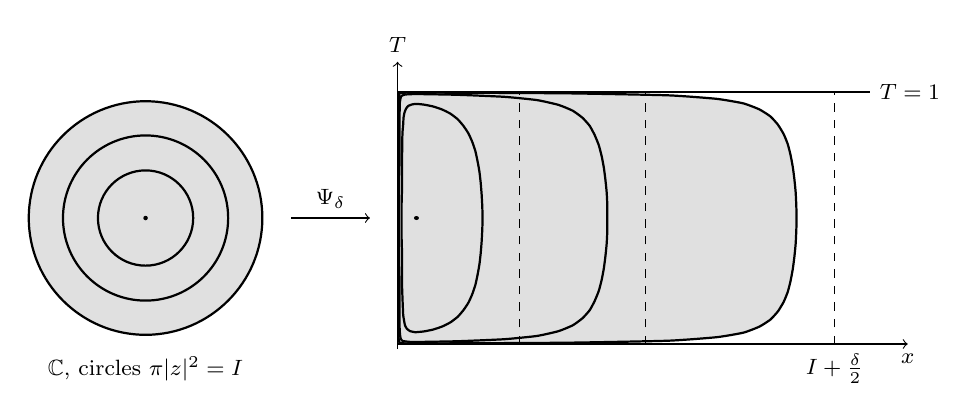
\begin{tikzpicture}[font=\footnotesize]
 \begin{scope}[scale=2.4]
  \fill[black!12] (0,0) circle (0.618);
  \draw[thick] (0,0) circle (0.252);
  \draw[thick] (0,0) circle (0.437);
  \draw[thick] (0,0) circle (0.618);
  \fill (0,0) circle (0.012);
  \node at (0,-0.8) {$\C$, circles $\pi|z|^2=I$};
 \end{scope}
 \draw[->] (1.85,0) -- node[above] {$\Psi_\delta$} (2.85,0);
 \begin{scope}[shift={(3.2,-1.6)},x=4cm,y=3.2cm]
  \fill[black!12] plot[smooth cycle,tension=0.3] coordinates {(0.060,0.002) (0.529,0.005) (0.858,0.013) (1.013,0.027) (1.098,0.045) (1.149,0.069) (1.184,0.097) (1.208,0.130) (1.226,0.167) (1.239,0.207) (1.248,0.251) (1.255,0.298) (1.260,0.346) (1.264,0.397) (1.266,0.448) (1.267,0.500) (1.266,0.552) (1.264,0.603) (1.260,0.654) (1.255,0.702) (1.248,0.749) (1.239,0.793) (1.226,0.833) (1.208,0.870) (1.184,0.903) (1.149,0.931) (1.098,0.955) (1.013,0.973) (0.858,0.987) (0.529,0.995) (0.060,0.998) (0.009,0.996) (0.005,0.989) (0.004,0.977) (0.003,0.960) (0.003,0.937) (0.003,0.910) (0.003,0.879) (0.003,0.843) (0.003,0.803) (0.003,0.760) (0.003,0.714) (0.003,0.666) (0.003,0.616) (0.003,0.565) (0.003,0.513) (0.003,0.461) (0.003,0.409) (0.003,0.359) (0.003,0.310) (0.003,0.262) (0.003,0.218) (0.003,0.177) (0.003,0.139) (0.003,0.105) (0.003,0.076) (0.003,0.051) (0.003,0.031) (0.004,0.016) (0.006,0.006) (0.026,0.002)};
  \draw[thick] plot[smooth cycle,tension=0.3] coordinates {(0.060,0.047) (0.084,0.050) (0.112,0.057) (0.141,0.069) (0.168,0.086) (0.191,0.108) (0.209,0.134) (0.225,0.164) (0.237,0.197) (0.247,0.234) (0.254,0.274) (0.260,0.316) (0.264,0.360) (0.267,0.406) (0.269,0.453) (0.270,0.500) (0.269,0.547) (0.267,0.594) (0.264,0.640) (0.260,0.684) (0.254,0.726) (0.247,0.766) (0.237,0.803) (0.225,0.836) (0.209,0.866) (0.191,0.892) (0.168,0.914) (0.141,0.931) (0.112,0.943) (0.084,0.950) (0.060,0.953) (0.047,0.951) (0.034,0.945) (0.027,0.934) (0.022,0.918) (0.019,0.898) (0.018,0.873) (0.016,0.844) (0.015,0.812) (0.015,0.776) (0.014,0.737) (0.014,0.695) (0.014,0.651) (0.014,0.606) (0.013,0.559) (0.013,0.512) (0.013,0.464) (0.013,0.417) (0.014,0.371) (0.014,0.327) (0.014,0.284) (0.014,0.244) (0.015,0.206) (0.016,0.172) (0.017,0.141) (0.018,0.114) (0.021,0.091) (0.024,0.073) (0.030,0.060) (0.040,0.051) (0.055,0.047)};
  \draw[dashed] (0.388,0) -- (0.388,1);
  \draw[thick] plot[smooth cycle,tension=0.3] coordinates {(0.060,0.008) (0.191,0.011) (0.339,0.019) (0.443,0.032) (0.511,0.051) (0.556,0.074) (0.587,0.102) (0.610,0.134) (0.626,0.171) (0.639,0.211) (0.648,0.254) (0.655,0.300) (0.660,0.348) (0.664,0.398) (0.666,0.449) (0.666,0.500) (0.666,0.551) (0.664,0.602) (0.660,0.652) (0.655,0.700) (0.648,0.746) (0.639,0.789) (0.626,0.829) (0.610,0.866) (0.587,0.898) (0.556,0.926) (0.511,0.949) (0.443,0.968) (0.339,0.981) (0.191,0.989) (0.060,0.992) (0.024,0.990) (0.012,0.984) (0.009,0.972) (0.007,0.955) (0.007,0.932) (0.006,0.905) (0.006,0.874) (0.006,0.839) (0.006,0.799) (0.006,0.757) (0.006,0.712) (0.005,0.664) (0.005,0.615) (0.005,0.564) (0.005,0.513) (0.005,0.461) (0.005,0.410) (0.005,0.360) (0.005,0.312) (0.006,0.265) (0.006,0.221) (0.006,0.181) (0.006,0.143) (0.006,0.110) (0.006,0.081) (0.007,0.056) (0.008,0.036) (0.010,0.022) (0.016,0.012) (0.043,0.008)};
  \draw[dashed] (0.788,0) -- (0.788,1);
  \draw[thick] plot[smooth cycle,tension=0.3] coordinates {(0.060,0.002) (0.529,0.005) (0.858,0.013) (1.013,0.027) (1.098,0.045) (1.149,0.069) (1.184,0.097) (1.208,0.130) (1.226,0.167) (1.239,0.207) (1.248,0.251) (1.255,0.298) (1.260,0.346) (1.264,0.397) (1.266,0.448) (1.267,0.500) (1.266,0.552) (1.264,0.603) (1.260,0.654) (1.255,0.702) (1.248,0.749) (1.239,0.793) (1.226,0.833) (1.208,0.870) (1.184,0.903) (1.149,0.931) (1.098,0.955) (1.013,0.973) (0.858,0.987) (0.529,0.995) (0.060,0.998) (0.009,0.996) (0.005,0.989) (0.004,0.977) (0.003,0.960) (0.003,0.937) (0.003,0.910) (0.003,0.879) (0.003,0.843) (0.003,0.803) (0.003,0.760) (0.003,0.714) (0.003,0.666) (0.003,0.616) (0.003,0.565) (0.003,0.513) (0.003,0.461) (0.003,0.409) (0.003,0.359) (0.003,0.310) (0.003,0.262) (0.003,0.218) (0.003,0.177) (0.003,0.139) (0.003,0.105) (0.003,0.076) (0.003,0.051) (0.003,0.031) (0.004,0.016) (0.006,0.006) (0.026,0.002)};
  \draw[dashed] (1.388,0) -- (1.388,1);
  \draw (0,0) -- (1.5,0);
  \draw (0,1) -- (1.5,1) node[right] {$T=1$};
  \draw[->] (0,-0.02) -- (0,1.12) node[above] {$T$};
  \draw[->] (0,0) -- (1.62,0) node[below] {$x$};
  \fill (0.06,0.5) circle (0.008);
  \node[below] at (1.388,0) {$I+\frac\delta2$};
 \end{scope}
\end{tikzpicture}
\caption{The disc-to-strip map $\Psi_\delta$ of Proposition~\ref{prop:str-strip}: computed level sets for $b_{\rm st}=\delta/\pi=0.12$
and $I=0.2,\,0.6,\,1.2$. The circle of area $I$ goes to the level set $\{R_{\rm st}+V_{\rm st}=\mathcal E_{\rm st}(I)\}$, which
encloses area $I$ and lies in $\{x<I+\frac\delta2\}$ (dashed lines); the dot is the common minimum $(b_{\rm st}/2,\frac12)$. The axes $x$ and $T$ have different scales.}
\label{fig:str-strip}
\end{figure}

\begin{proof}
(i), (ii) Apply Lemma~\ref{lem:str-normalisation}(iii) to the smooth positive density
$\mathcal J_{\rm st}$ and $F_{\rm st}$. The latter is given by Lemma~\ref{lem:str-morse-inverse}(iv),
and $\mathfrak a_{\rm st}\to\infty$ by Lemma~\ref{lem:str-area}(iii). The level
identity follows from $R_{\rm st}\circ X_{\rm st}+V_{\rm st}\circ Y_{\rm st}=|\xi|^2$.
(iii) Let $I=\pi|z|^2$ and $\mathcal E=\mathcal E_{\rm st}(I)$. By Lemma~\ref{lem:str-area}(iii),
$I=\mathfrak a_{\rm st}(\mathcal E)\ge\mathcal E-b_{\rm st}(\frac\pi2-1)$. By (ii) and $V_{\rm st}\ge0$, $R_{\rm st}(x)\le\mathcal E$, so by
Lemma~\ref{lem:str-area}(i)
\[
 x\le x_+(\mathcal E)<\mathcal E+b_{\rm st}\le I+b_{\rm st}\tfrac\pi2=I+\tfrac\delta2 .
\]
Positivity of $x$ and $0<T<1$ hold because $\Psi_\delta$ takes values in the strip.
(iv) Let $\mathcal E=\mathcal E_{\rm st}(\pi|z|^2)$. Since $\mathcal E_{\rm st}$ is increasing, $\mathcal E\le\mathcal E_{\rm st}(I_{\max})$, and
$I_{\max}=\mathfrak a_{\rm st}(\mathcal E_{\rm st}(I_{\max}))\ge\mathcal E_{\rm st}(I_{\max})-b_{\rm st}(\frac\pi2-1)$ by
Lemma~\ref{lem:str-area}(iii); so $\mathcal E\le\mathcal E_{\max}$. By (ii), $R_{\rm st}(x)\le\mathcal E_{\max}$ and
$V_{\rm st}(T)\le\mathcal E_{\max}$. The first bound is $x\ge x_-(\mathcal E_{\max})>0$ (Lemma~\ref{lem:str-area}(i)). The second
says $2\sqrt{T(1-T)}\ge(1+\mathcal E_{\max}/b_{\rm st})^{-1}$, i.e.\
$(T-\frac12)^2=\frac14-T(1-T)\le\frac14\big[1-(1+\mathcal E_{\max}/b_{\rm st})^{-2}\big]$.
\end{proof}

%----------------------------------------------------------------------
\subsection{Enlarged capacities and the ball estimate}\label{sec:str-balls}

Throughout the remaining layer construction we work in the situation of \Mref{Theorem}{thm:mech-packing} with $n\ge3$: a model input
(\Mref{Definition}{def:mech-model}) of rank $m=n-1$ with handle data (\Mref{Definition}{def:hdl-handle-data}), capacities $a_1,\dots,a_k>0$ with
$\{p\in\R^m_{\ge0}:|p|\le a_i\}\subset\tau_\Delta\Delta$ for some $\tau_\Delta<1$, a function $P$ and a comparison datum
$(K,q)$ with gap $\gamma>0$, and capacities $\rho_i<a_i$. The outer faces of $\Delta$ are $\{\langle b_\nu,p\rangle=\ell_\nu\}$,
$1\le\nu\le N$, with $\ell_\nu>0$. The caps $h_i$ are those of (\Mnum{eq:hdl-caps}) with $\rho_i^\sharp=\hat\rho_i$
($\hat\rho_i$ is defined in Definition~\ref{def:str-enlarged} below). By \Mref{Proposition}{prop:hdl-layers}(i), each $h_i$
is smooth on $\R^m$ and
\begin{equation}\label{eq:str-cap}
 0\le h_i(p),\qquad (a_i+\hat\rho_i)/2-|p|\le h_i(p)\qquad(p\in\R^m).
\end{equation}

\begin{lemma}[Interior of the fibre polytope]\label{lem:str-int}
\uses{M-def:mech-model}
Let $V_\Delta=\{w\in\C^m:\langle b_\nu,p(w)\rangle\le\ell_\nu\ \text{for all }\nu\}$. Then
\begin{equation}\label{eq:str-int}
 \operatorname{int}V_\Delta=\{w\in\C^m:\langle b_\nu,p(w)\rangle<\ell_\nu\ \text{for all }\nu\},
\end{equation}
and $\{w:|p(w)|\le a_i\}\subset\operatorname{int}V_\Delta$ for $1\le i\le k$.
\end{lemma}

\begin{proof}
The right side of \eqref{eq:str-int} is open and contained in $V_\Delta$. If $\langle b_\nu,p(w)\rangle=\ell_\nu>0$ for some $\nu$,
then $\langle b_\nu,p((1+t)w)\rangle=(1+t)^2\ell_\nu>\ell_\nu$ for $t>0$, so $w$ is not an interior point. If $|p(w)|\le a_i$, then
$p(w)\in\tau_\Delta\Delta$, so $\langle b_\nu,p(w)\rangle\le\tau_\Delta\ell_\nu<\ell_\nu$ for all $\nu$.
\end{proof}

The margin $a_i-\rho_i=2\delta_i$ gives nested source balls and a positive gap between
the strip image and the cap. We use strip parameter $\varepsilon_i=\delta_i/8$, whose excess
is less than $\delta_i/16$.

\begin{definition}[Enlarged capacities]\label{def:str-enlarged}
\lean{SymplecticPacking.HighDim.RawToricModel.packingSource,
SymplecticPacking.Branch2.CubicData.rhoBar, SymplecticPacking.Branch2.CubicData.deltaStrip,
SymplecticPacking.Branch2.CubicData.rhoHat}
For $1\le i\le k$ put
\[
 \delta_i=\frac{a_i-\rho_i}2,\qquad
 \bar\rho_i=a_i-\frac34\delta_i,\qquad \hat\rho_i=a_i-\frac{\delta_i}2 .
\]
Here $\bar\rho_i$ is the closed enlarged source capacity and $\hat\rho_i$ the open domain capacity, and
$\rho_i<\frac{\rho_i+a_i}2=a_i-\delta_i<\bar\rho_i<\hat\rho_i<a_i$. Put
$\varepsilon_i=(a_i-\hat\rho_i)/4=\delta_i/8$; the $i$-th ball is placed by $\Psi_{\varepsilon_i}$.
In the four-dimensional branch (\S\ref{sec:shd-four}) the same letters denote different values:
there $\bar\rho_i=(\rho_i+a_i)/2=a_i-\delta_i$, $\hat\rho_i=a_i-\frac34\delta_i$, and the $i$-th ball is placed by
$\Psi_{\delta_i}$ (Proposition~\ref{prop:shd4-maps}). The two branches never occur together, and each section states which
values it uses.
\end{definition}

\begin{lemma}[Ball estimate]\label{lem:str-ball}
\lean{SymplecticPacking.HighDim.ToricPackingStages.thinPlanar_bound,
SymplecticPacking.HighDim.ToricPackingStages.smoothCap_ge,
SymplecticPacking.Strip.Cubic.x_lt_hi}
\uses{prop:str-strip, def:str-enlarged, lem:str-int, M-prop:hdl-layers}
Let $1\le i\le k$, $(z_{\rm b},z_{\rm f})\in\C\times\C^m$, $\varpi=\pi|z_{\rm b}|^2$, $p=p(z_{\rm f})$, and let $x$ be the first
component of $\Psi_{\varepsilon_i}(z_{\rm b})$.
\begin{enumerate}[label=(\alph*)]
\item If $\varpi+|p|\le a_i-\delta_i$, then
\begin{equation}\label{eq:str-ball}
 x<\varpi+\frac{\delta_i}{16}\le a_i-|p|-\frac{15\delta_i}{16}
 \le h_i(p)-\frac{11\delta_i}{16}<h_i(p)-\frac{\delta_i}2 .
\end{equation}
\item If $\varpi+|p|\le\bar\rho_i$, then $x<a_i-|p|-\frac{11\delta_i}{16}\le h_i(p)-\frac{7\delta_i}{16}<h_i(p)-\frac{\delta_i}4$.
\item If $\varpi+|p|<\hat\rho_i$, then $x<a_i-|p|-\frac{7\delta_i}{16}\le h_i(p)-\frac{3\delta_i}{16}<h_i(p)$.
\end{enumerate}
In each case $|p|<a_i$, hence $z_{\rm f}\in\operatorname{int}V_\Delta$.
\end{lemma}

\begin{proof}
By \eqref{eq:str-x-bound}, $x<\varpi+\varepsilon_i/2=\varpi+\delta_i/16$. (a) $\varpi\le a_i-\delta_i-|p|=a_i-|p|-\delta_i$. (b)
$\varpi\le\bar\rho_i-|p|=a_i-|p|-\frac34\delta_i$. (c) $\varpi<\hat\rho_i-|p|=a_i-|p|-\frac12\delta_i$. In each case the
cap comparison is \eqref{eq:str-cap} in the form $a_i-\delta_i/4-|p|\le h_i(p)$. Finally $|p|\le\varpi+|p|<a_i$, and the last
assertion is Lemma~\ref{lem:str-int}.
\end{proof}

The base factor is placed by $\Psi_{\varepsilon_i}$, which is not toric, and the fibre level $p$ enters only through the bound
$x<h_i(p)$.

%----------------------------------------------------------------------
\subsection{Layer coordinates}\label{sec:str-layer-coords}

We recall the objects of \Msec{sec:hdl} and \S\ref{sec:shd} used here. In the product coordinates of
\Mref{Definition}{def:hdl-handle-data}, $E|_{\mathcal A^+}\cong\mathcal A^+\times\C^m$ with base coordinates $(s,v)$ and fibre
coordinate $w$, and $\omega_V=\sum_jdp_j\wedge d\theta_j$. The one-form $\beta$ equals $b(v)\,dv$ on $\mathcal A^+$, where $b\ge0$
is smooth, $b>0$ exactly on $(v_-,v_+)$ and $\int b=1$. The layer intervals $I_j=[l_j,r_j]\subset(0,1)$,
$1\le j\le k$, and the residual interval $I_*$ are pairwise disjoint, with flat steps $\varsigma_j$ rising from $0$ to $1$ across
$I_j$ ($\varsigma_j'\ge0$). By Proposition~\ref{prop:shd-layer-path}, the final coefficient $G_{\rm f}$ satisfies, on
$I_i\times\C^m$,
\begin{equation}\label{eq:str-Gf}
 G_{\rm f}(s,w)=A_i(p(w))+\varsigma_i(s)h_i(p(w)),\qquad A_i=J+\sum_{j<i}h_j ,
\end{equation}
where $J=K-H^*=K-\Hb+\epsilon_{\rm sm}$ is the collar coefficient of (\Mnum{eq:hdl-caps}). The function $K$ is smooth on an open
neighbourhood of $\Delta$ in $\R^m$ (\Mref{Definition}{def:mech-datum}) and the $h_j$ are smooth on $\R^m$. The functions
$\Hb(p)=\int_{\Sigma_\ell}\kappa(p)$ and $\epsilon_{\rm sm}(p)=\int_{\Sigma_\ell}\kappa_{\rm sm}(p)$ are smooth on an open neighbourhood of $\Delta$ as
well: $\kappa(p)$ extends smoothly in the moment variables (\Mref{Definition}{def:mech-model}), $\kappa_{\rm sm}(p)$ is obtained from it by
multiplying by the fixed cutoff $\chi_\partial$ and adding the $p$-independent form $(1-\chi_\partial)e_\Lambda\Lambda$
(see equation~\Mnum{eq:hdl-ksm}), and $\Sigma_\ell$ is compact, so one may differentiate under the integral sign. Hence $A_i$ is smooth on an
open neighbourhood $W$ of $\Delta$ in $\R^m$. Write $\Lambda=a_\Lambda(s,v)\,ds\wedge dv$ with $a_\Lambda>0$ on $\mathcal A^+$ and put
$\ell_0(s,v)=e_\Lambda a_\Lambda(s,v)>0$. On $E|_{\mathcal A}$, over a neighbourhood of $V_\Delta$, the twisted form is
given by (\Mnum{eq:hdl-final}) (Proposition~\ref{prop:shd-layer-path}),
\begin{equation}\label{eq:str-pre}
 \Omega_{\rm pre}=\omega_V+e_\Lambda\Lambda+d(G_{\rm f}\beta)=\omega_V+\ell_0(s,v)\,ds\wedge dv+d(G_{\rm f}\beta),\qquad
 \Omega_{\rm final}=\mathcal D^*\Omega_{\rm pre}.
\end{equation}
The $i$-th layer is the open set
\[
 \Lambda_i=\{(s,v,w):l_i<s<r_i,\ v_-<v<v_+,\ w\in\operatorname{int}V_\Delta\}\subset E|_{\mathcal A}.
\]

On $\Lambda_i$ only the $i$-th step is moving: the lower steps already equal $1$ and contribute the toric function $A_i$,
the upper ones vanish. The coordinate $T$ integrates $\beta$, and the coordinate $x_i$ integrates the background area in
the $s$-direction and adds the height $\varsigma_ih_i$ by which the $i$-th step has risen.

\begin{construction}[Layer coordinates]\label{cons:str-layer-coords}
\lean{SymplecticPacking.HighDim.ToricPackingStages.layerCoord,
SymplecticPacking.HighDim.ToricPackingStages.layerDensity,
SymplecticPacking.Strip.Tcoord, SymplecticPacking.Strip.Cubic.layerX}
\uses{M-def:hdl-handle-data, M-prop:hdl-layers}
Let $T(v)=\int_{v_-}^vb(t)\,dt$ for $v_-<v<v_+$, an increasing diffeomorphism onto $(0,1)$ with $dT=\beta$, and $v(T)$ its
inverse. For $0<s<1$, $0<T<1$ and $p\in\R^m$ put
\begin{align*}
 \ell(s,T)&=\frac{\ell_0(s,v(T))}{b(v(T))},&
 L_i(s,T)&=\int_{l_i}^s\ell(u,T)\,du,\\
 x_i(s,T,p)&=L_i(s,T)+\varsigma_i(s)h_i(p),&
 x_i^+(T,p)&=x_i(r_i,T,p).
\end{align*}
This is the coordinate (\Mnum{eq:hdl-layer-x}). On $\Lambda_i$ the layer chart is
\[
 \kappa_i(s,v,w)=\big(x_i(s,T(v),p(w)),\,T(v),\,w\big),
\]
and
\[
 \mathcal U_i=\big\{(x,T,w)\in\R\times(0,1)\times\operatorname{int}V_\Delta:\ 0<x<x_i^+(T,p(w))\big\}.
\]
\end{construction}

\begin{lemma}[Layer root]\label{lem:str-layer-root}
\lean{SymplecticPacking.Strip.Cubic.layerX_deriv, SymplecticPacking.Strip.Cubic.layerRoot,
 SymplecticPacking.Strip.Cubic.layerRoot_existsUnique, SymplecticPacking.Strip.Cubic.layerRoot_mem,
 SymplecticPacking.Strip.Cubic.layerChart_layerCoord, SymplecticPacking.Strip.Cubic.layerCoord_layerChart,
 SymplecticPacking.Strip.Cubic.contDiffAt_layerCoord, SymplecticPacking.Strip.Cubic.layerChart_smooth,
SymplecticPacking.HighDim.ToricPackingStages.layerChartInv_local_spec}
\uses{cons:str-layer-coords}
\begin{enumerate}[label=(\roman*)]
\item $x_i$ is smooth on $(0,1)\times(0,1)\times\R^m$, and
$\partial_sx_i=\ell(s,T)+\varsigma_i'(s)h_i(p)\ge\ell(s,T)>0$. Moreover $x_i(l_i,T,p)=0$ and
$x_i^+(T,p)=L_i(r_i,T)+h_i(p)>h_i(p)$.
\item For $0<T<1$, $w\in\operatorname{int}V_\Delta$ and $0<x<x_i^+(T,p(w))$ there is a unique
$s=\sigma_i(x,T,p(w))\in(l_i,r_i)$ with $x_i(s,T,p(w))=x$. This root is smooth as a function
of $(x,T,w)$ on that open domain, including the fibre coordinate axes.
\item $\kappa_i$ is a diffeomorphism of $\Lambda_i$ onto $\mathcal U_i$, with inverse
$(x,T,w)\mapsto\big(\sigma_i(x,T,p(w)),\,v(T),\,w\big)$.
\end{enumerate}
\end{lemma}

\begin{proof}
(i) $v(T)$ is smooth because $T'(v)=b(v)>0$ on $(v_-,v_+)$, so $L_i$ is smooth; $\varsigma_i$ and $h_i$ are smooth. The derivative
formula is immediate, and $\varsigma_i'\ge0$, $h_i\ge0$ by \eqref{eq:str-cap}. At $s=l_i$, $L_i=0$ and $\varsigma_i=0$; at $s=r_i$,
$\varsigma_i=1$ and $L_i(r_i,T)>0$ because $\ell>0$ and $r_i>l_i$.
(ii) By (i), $s\mapsto x_i(s,T,p)$ is strictly increasing on $[l_i,r_i]$ from $0$ to $x_i^+(T,p)$, which gives existence and
uniqueness of the root in $(l_i,r_i)$. The set of $(x,T,w)$ in question is open because $x_i^+$ and $p(w)$ are continuous. Near any of its
points the implicit function theorem ($\partial_sx_i>0$) gives a smooth local solution, which coincides with the root by
uniqueness. The moment map is smooth in Cartesian coordinates, so this also holds at its axes.
(iii) $\kappa_i$ is smooth since $p(w)$ is smooth in Cartesian coordinates. For fixed $(v,w)$ the first component increases
strictly from $0$ to $x_i^+(T(v),p(w))$ as $s$ runs over $(l_i,r_i)$, and $T$ is a bijection $(v_-,v_+)\to(0,1)$; hence
$\kappa_i$ is a bijection $\Lambda_i\to\mathcal U_i$, $\mathcal U_i$ is open, and the inverse is the stated map, which is smooth
by (ii).
\end{proof}

\begin{lemma}[The form on a layer]\label{lem:str-layer-form}
\lean{SymplecticPacking.Strip.Cubic.Gf_on_layer, SymplecticPacking.Strip.Cubic.layer_form,
SymplecticPacking.HighDim.ToricPackingStages.weightedLayerMap_spec}
\uses{cons:str-layer-coords, M-prop:hdl-layers}
On $\Lambda_i$, $\Omega_{\rm pre}=\omega_V+dx_i\wedge dT+dA_i(p)\wedge dT$, where $x_i=x_i(s,T(v),p(w))$; equivalently
$(\kappa_i^{-1})^*\Omega_{\rm pre}=\omega_V+dx\wedge dT+dA_i(p)\wedge dT$ on $\mathcal U_i$.
\end{lemma}

\begin{proof}
On $\Lambda_i$ we have $\beta=dT$ and $ds\wedge dv=b^{-1}ds\wedge dT$. Since $\beta$ is closed and $G_{\rm f}$ does not depend on
$v$, \eqref{eq:str-pre} and \eqref{eq:str-Gf} give
\[
 \Omega_{\rm pre}=\omega_V+\ell(s,T)\,ds\wedge dT+\big(\varsigma_i'h_i\,ds+dA_i+\varsigma_i\,dh_i\big)\wedge dT ,
\]
with $A_i$, $h_i$ evaluated at $p(w)$. On the other hand
$dx_i\wedge dT=\big(\partial_sL_i+\varsigma_i'h_i\big)\,ds\wedge dT+\varsigma_i\,dh_i\wedge dT$, because the $dT$-component of $dx_i$
drops out, and $\partial_sL_i=\ell(s,T)$. Subtracting gives the claim.
\end{proof}

%----------------------------------------------------------------------
\subsection{The layer maps}\label{sec:str-layer-maps}

The term $dA_i(p)\wedge dT$ couples the fibre to the $T$-direction. It is removed by the multi-angle shear
$\mathrm{Sh}_{A_i}(x,T,w)=(x,T,\mathrm{Sh}_{A_i,T}(w))$ of Lemma~\ref{lem:hdl-shear}, applied with $A=A_i$ on $W$:
\[
 \mathrm{Sh}_{A_i,T}(w)_j=\exp\big(-2\pi i\,T\,\partial_jA_i(p(w))\big)\,w_j\qquad(1\le j\le m).
\]
It preserves $x$, $T$ and $p$, hence maps $\mathcal U_i$ diffeomorphically onto itself (its inverse, the same formula with
$+2\pi i$, also preserves $\mathcal U_i$), and
$\mathrm{Sh}_{A_i}^*\big(\omega_V+dx\wedge dT+dA_i(p)\wedge dT\big)=\omega_V+dx\wedge dT$.

\begin{construction}[Layer maps]\label{cons:str-layer-map}
\lean{SymplecticPacking.HighDim.ToricPackingStages.weightedLayerMap,
SymplecticPacking.HighDim.RawToricModel.layerMapsOf, SymplecticPacking.Strip.Cubic.layerMap}
\uses{cons:str-map, def:str-enlarged, lem:str-layer-root, lem:hdl-shear}
For $1\le i\le k$ and $(z_{\rm b},z_{\rm f})\in\Bo(\hat\rho_i)$ put $(x,T)=\Psi_{\varepsilon_i}(z_{\rm b})$, $p=p(z_{\rm f})$ and
\[
 E_i(z_{\rm b},z_{\rm f})=\Big(\sigma_i(x,T,p),\ v(T),\ \mathrm{Sh}_{A_i,T}(z_{\rm f})\Big)
 =\kappa_i^{-1}\circ\mathrm{Sh}_{A_i}\circ(\Psi_{\varepsilon_i}\times\mathrm{id})\,(z_{\rm b},z_{\rm f}) .
\]
\end{construction}

\begin{proposition}[Layer maps]\label{prop:str-layer}
\lean{SymplecticPacking.HighDim.ToricPackingStages.weightedLayerMap_spec,
SymplecticPacking.HighDim.ToricPackingStages.layerMapsOf_spec_of_normal_form,
SymplecticPacking.HighDim.RawModelAgreement.native_layerMaps_spec,
SymplecticPacking.Strip.Cubic.layerMap_symplectic,
SymplecticPacking.Strip.Cubic.layerMap_disjoint}
\uses{cons:str-layer-map, lem:str-ball, lem:str-layer-root, lem:str-layer-form, prop:str-strip, lem:hdl-shear}
For $1\le i\le k$:
\begin{enumerate}[label=(\roman*)]
\item $E_i$ is well defined and smooth on $\Bo(\hat\rho_i)$, which contains $B(\bar\rho_i)\supset B(a_i-\delta_i)$, and is a
diffeomorphism onto an open subset of $\Lambda_i$, with inverse
\[
 E_i^{-1}(s,v,w)=\Big(\Psi_{\varepsilon_i}^{-1}\big(x_i(s,T,p(w)),\,T\big),\ \mathrm{Sh}_{A_i,T}^{-1}(w)\Big),\qquad T=T(v);
\]
\item $E_i^*\Omega_{\rm pre}=\omega_0$;
\item $E_i(\Bo(\hat\rho_i))$ lies over the base rectangle $(l_i,r_i)\times(v_-,v_+)\subset\mathcal A$ and in
$\{|p|<a_i\}\subset\operatorname{int}V_\Delta$;
\item on $B(\bar\rho_i)$ the coordinate $x=x_i\circ E_i$ satisfies $x<h_i(p)-\delta_i/4$, and on $B(a_i-\delta_i)$ it satisfies
$x<h_i(p)-\delta_i/2$; the set $E_i(B(\bar\rho_i))$ is a compact subset of $\Lambda_i$;
\item the images $E_i(\Bo(\hat\rho_i))$, $1\le i\le k$, are pairwise disjoint.
\end{enumerate}
\end{proposition}

\begin{proof}
(i) By Lemma~\ref{lem:str-ball}(c), for $(z_{\rm b},z_{\rm f})\in\Bo(\hat\rho_i)$ we have $z_{\rm f}\in\operatorname{int}V_\Delta$ and
$0<x<h_i(p)<x_i^+(T,p)$ (Lemma~\ref{lem:str-layer-root}(i)), and $0<T<1$ by \eqref{eq:str-x-bound}. Hence
$\Psi_{\varepsilon_i}\times\mathrm{id}$, a diffeomorphism of $\C\times\C^m$ onto $(0,\infty)\times(0,1)\times\C^m$
(Proposition~\ref{prop:str-strip}(i)), maps the open set $\Bo(\hat\rho_i)$ diffeomorphically onto an open subset of
$\mathcal U_i$. The shear $\mathrm{Sh}_{A_i}$ is a diffeomorphism of $\mathcal U_i$ onto itself, and $\kappa_i^{-1}$ a diffeomorphism
of $\mathcal U_i$ onto $\Lambda_i$ (Lemma~\ref{lem:str-layer-root}(iii)). So $E_i$ is a diffeomorphism of $\Bo(\hat\rho_i)$ onto
an open subset of $\Lambda_i$, and composing the three inverses gives the formula, using that $\mathrm{Sh}_{A_i,T}^{-1}$ preserves $p$.
The inclusions of balls hold because $a_i-\delta_i<\bar\rho_i<\hat\rho_i$.

(ii) By Lemma~\ref{lem:str-layer-form}, $(\kappa_i^{-1})^*\Omega_{\rm pre}=\omega_V+dx\wedge dT+dA_i(p)\wedge dT$ on $\mathcal U_i$.
By Lemma~\ref{lem:hdl-shear} and Proposition~\ref{prop:str-strip}(i),
\begin{align*}
 E_i^*\Omega_{\rm pre}
 &=(\Psi_{\varepsilon_i}\times\mathrm{id})^*\mathrm{Sh}_{A_i}^*
      \big(\omega_V+dx\wedge dT+dA_i(p)\wedge dT\big)\\
 &=(\Psi_{\varepsilon_i}\times\mathrm{id})^*\big(\omega_V+dx\wedge dT\big)\\
 &=\omega_V(z_{\rm f})+\omega_\C(z_{\rm b})=\omega_0 .
\end{align*}

(iii) The $s$-component $\sigma_i(x,T,p)$ lies in $(l_i,r_i)$ and $v(T)\in(v_-,v_+)$; the fibre component has the same $p$ as
$z_{\rm f}$, and $|p|<a_i$ by Lemma~\ref{lem:str-ball}.

(iv) The two bounds are Lemma~\ref{lem:str-ball}(b) and (a), since $x_i\circ E_i$ is the first component of
$\Psi_{\varepsilon_i}(z_{\rm b})$ and the shear preserves $p$. The closed ball $B(\bar\rho_i)$ is compact and contained in the domain of
the continuous map $E_i$, whose values lie in $\Lambda_i$.

(v) The $s$-components of points of different images lie in the disjoint open intervals $(l_i,r_i)$.
\end{proof}

For $(z_{\rm b},z_{\rm f})\in B(\bar\rho_i)$, Proposition~\ref{prop:str-strip}(iv) with $I_{\max}=\bar\rho_i$ and
$b_{\rm st}=\varepsilon_i/\pi$ bounds $\Psi_{\varepsilon_i}(z_{\rm b})$ away from the edges $x=0$ and $T\in\{0,1\}$ by explicit constants, and
$|p|\le\bar\rho_i<a_i$. These are the margins entering the effective data of \S\ref{sec:efd}.

%----------------------------------------------------------------------
\subsection{Undoing the twist and the Moser map}\label{sec:str-embeddings}

The layer maps land in $(\Lambda_i,\Omega_{\rm pre})$. To reach $(E,\Omega)$ we undo the twist $\mathcal D$, which turned
$\Omega_{\rm pre}$ into $\Omega_{\rm final}$, and then the Moser map $\Phi$, which turned $\Omega_{\rm final}$ into $\Omega$.

\begin{lemma}[The twist and the Moser map]\label{lem:str-DPhi}
\uses{prop:shd-layer-path, prop:shd-moser, M-prop:hdl-faces}
\begin{enumerate}[label=(\roman*)]
\item[(D)] The twist $\mathcal D(s,v,w)=(s,v,q_{f(s)}(w))$ restricts to a diffeomorphism of
$\{(s,v,w)\in E|_{\mathcal A}:w\in\operatorname{int}V_\Delta\}$ onto itself which fixes base points, with inverse
$\mathcal D^{-1}(s,v,w)=(s,v,q_{f(s)}^{-1}(w))$, and $(\mathcal D^{-1})^*\Omega_{\rm final}=\Omega_{\rm pre}$ there.
\item[($\Phi$)] $\Phi=\Phi_2\circ\Phi_1\circ\Phi_0$ is a diffeomorphism of $E$ which maps $V_\Delta(E)$ and its interior
$\operatorname{int}V_\Delta(E)$ onto themselves, and $\Phi^*\Omega_{\rm final}=\Omega$ on $V_\Delta(E)$.
\end{enumerate}
\end{lemma}

\begin{proof}
(D) The map $(t,w)\mapsto q_t(w)$ is smooth and each $q_t$ is a diffeomorphism of $\C^m$ with $q_t(V_\Delta)=V_\Delta$
(\Mref{Definition}{def:mech-datum}); a homeomorphism which preserves a set preserves its interior, so
$q_t(\operatorname{int}V_\Delta)=\operatorname{int}V_\Delta$. Hence $\mathcal D$ and the displayed inverse are smooth maps of the
stated set into itself, inverse to each other, and they fix base points. Since $\Omega_{\rm final}=\mathcal D^*\Omega_{\rm pre}$ on
$E|_{\mathcal A}$ by \eqref{eq:str-pre}, $(\mathcal D^{-1})^*\Omega_{\rm final}=\Omega_{\rm pre}$.

($\Phi$) Each $\Phi_j$ is the time-one map of a smooth vector field with compact support, hence a diffeomorphism of $E$ whose
inverse is the backward flow. By \Mref{Proposition}{prop:hdl-faces} and Proposition~\ref{prop:shd-moser}, each $\Phi_j$ maps the
model region $V_\Delta(E)$ and its interior onto themselves and satisfies $\Phi_j^*\Omega_{j,1}=\Omega_{j,0}$ there, where
$\Omega_{0,0}=\Omega$, $\Omega_{j,1}=\Omega_{j+1,0}$ and $\Omega_{2,1}=\Omega_{\rm final}$. Composing gives
$\Phi^*\Omega_{\rm final}=\Phi_0^*\Phi_1^*\Phi_2^*\Omega_{2,1}=\Omega$ on $V_\Delta(E)$.
\end{proof}

\begin{proposition}[Embeddings into the model]\label{prop:str-embeddings}
\lean{SymplecticPacking.HighDim.RawModelAgreement.native_packing_spec,
SymplecticPacking.Strip.Cubic.fN_symplectic, SymplecticPacking.Strip.Cubic.fN_eq_imp,
SymplecticPacking.Strip.Cubic.fN_disjoint, SymplecticPacking.Strip.Cubic.fN_avoid_fibres}
\uses{prop:str-layer, lem:str-DPhi}
For $1\le i\le k$ let
\[
 \psi_i=\Phi^{-1}\circ\mathcal D^{-1}\circ E_i\colon\Bo(\hat\rho_i)\to E .
\]
Then:
\begin{enumerate}[label=(\roman*)]
\item $\psi_i$ is a smooth symplectic embedding of $(\Bo(\hat\rho_i),\omega_0)$ onto an open subset of
$(\operatorname{int}V_\Delta(E),\Omega)$; in particular it restricts to a symplectic embedding of a neighbourhood of
$B(\bar\rho_i)$, and $\psi_i(B(\bar\rho_i))$ is a compact subset of $\operatorname{int}V_\Delta(E)$;
\item the images $\psi_i(\Bo(\hat\rho_i))$, $1\le i\le k$, are pairwise disjoint.
\end{enumerate}
\end{proposition}

\begin{proof}
(i) By Proposition~\ref{prop:str-layer}(i),(iii), $E_i$ is a diffeomorphism of $\Bo(\hat\rho_i)$ onto an open subset of
$\Lambda_i$. By Lemma~\ref{lem:str-DPhi}(D), $\mathcal D^{-1}$ maps it diffeomorphically onto an open subset of
$E|_{\mathcal A}$ lying over $(l_i,r_i)\times(v_-,v_+)$ with fibre component in $\operatorname{int}V_\Delta$. Points of this base
rectangle have $b(v)>0$, so they lie in the support of $\beta$, which is contained in $\mathcal B\subset\operatorname{int}\Sigma_\ell$
(\Mref{Definition}{def:hdl-handle-data}); hence the image lies in $\operatorname{int}\Sigma_\ell\times\operatorname{int}V_\Delta
=\operatorname{int}V_\Delta(E)$. By
Lemma~\ref{lem:str-DPhi}($\Phi$), $\Phi^{-1}$ maps $\operatorname{int}V_\Delta(E)$ diffeomorphically onto itself. So $\psi_i$ is a
diffeomorphism onto an open subset of $\operatorname{int}V_\Delta(E)$, and
\[
 \psi_i^*\Omega=E_i^*(\mathcal D^{-1})^*(\Phi^{-1})^*\Omega=E_i^*(\mathcal D^{-1})^*\Omega_{\rm final}=E_i^*\Omega_{\rm pre}=\omega_0
\]
by Lemma~\ref{lem:str-DPhi} and Proposition~\ref{prop:str-layer}(ii). Since $\bar\rho_i<\hat\rho_i$, $\Bo(\hat\rho_i)$ is a
neighbourhood of the compact set $B(\bar\rho_i)$, whose image is compact.

(ii) The sets $E_i(\Bo(\hat\rho_i))$ are pairwise disjoint (Proposition~\ref{prop:str-layer}(v)). $\mathcal D^{-1}$ is one
injective map, the same for every $i$, so the sets $\mathcal D^{-1}E_i(\Bo(\hat\rho_i))$ are pairwise disjoint; the same holds
after applying the single injective map $\Phi^{-1}$.
\end{proof}

These maps are the higher-dimensional embeddings of Theorem~\ref{thm:shd-packing}.
For the periodic four-dimensional input, the upper caps, clocks and deck
coordinates give the maps of Remark~\ref{rem:shd-four}. Their images avoid the exceptional
fibres by the equivariant handle and layer identities of that construction.

\section{The finite-atlas toric construction}\label{sec:native-toric}

This section fixes the choices behind the higher-dimensional model maps of \Msec{sec:hdl}: the finite primitive operator,
the normalised primitive $\Gamma_n$, the three Moser fields and the maps $\psi_i$. The data are those of a higher-dimensional
model input with handle data (\Mref{Definition}{def:mech-model} and \Mref{Definition}{def:hdl-handle-data}): the physical primitive
$\Gamma_{\rm phys}(p)$ with curvature $\kappa(p)=d_\Sigma\Gamma_{\rm phys}(p)$, the reference primitive $\Gamma_{\rm ref}$ with
positive curvature $\Lambda$, the annular coordinate $s_{\rm a}$ of half-width $w$ with working half-width $b<w$, the closed
one-form $\beta$, the clock $f(s)=S(s)$, $s=(s_{\rm a}+b)/(2b)$, and the collar cutoff $\chi_\partial$. All forms are evaluated
in the explicit coordinates of the model curve. The \emph{correction atlas} is the finite family of rational coordinate boxes of
Definition~\ref{def:shd-presentation}; its inner boxes cover a compact subset of $\operatorname{int}\Sigma_\ell$, the
\emph{correction core}. These data satisfy: the support of $1-\chi_\partial$ in $\Sigma_\ell$ and the handle are contained
in the correction core, and the correction core is contained in the correction region of
\Mref{Definition}{def:hdl-handle-data}(d), on which $\kappa(p)\ge\kappa_-\Lambda$ for $p\in\Delta$. Its overlap tree has root
the box $0$, and every other box $i$ has a parent $j<i$. A second, larger finite atlas, the \emph{flow atlas}, covers the
whole closed model base.

\subsection{A fixed finite primitive operator}

Let $\zeta_i$ be the partition weights of the correction atlas ($\sum_i\zeta_i=1$ on the correction core, $\zeta_i$ supported in
box $i$), $\eta_i$ a unit-mass bump in box $i$, and $\eta_{ij}$ a unit-mass bump in the overlap of a child $i$ and its parent $j$.
Write $P_i$ for the rectangular primitive \eqref{eq:shd-Ploc} in box $i$; thus $dP_i\alpha=\alpha$ for every two-form $\alpha$
supported in box $i$ with zero coordinate mass, and $P_i\alpha$ is supported in box $i$ (Lemma~\ref{lem:shd-primitive}). Set
\[
 e_i=P_i(\eta_i-\eta_{ij})+P_j(\eta_{ij}-\eta_j),\qquad
 T_0=0,\qquad T_i=e_i+T_j .
\]
For a two-form $\omega$ supported in the correction core put
\[
 m_i(\omega)=\int\zeta_i\omega,\quad m(\omega)=\sum_i m_i(\omega),\qquad
 \mathcal P\omega=\sum_i\bigl[P_i(\zeta_i\omega-m_i(\omega)\eta_i)+m_i(\omega)T_i\bigr],
\]
where $\int\zeta_i\omega$ is the coordinate integral in box $i$. Each argument of $P_i$ has zero coordinate mass, and
$de_i=\eta_i-\eta_j$; by induction along the tree, $dT_i=\eta_i-\eta_0$. Hence
\[
 d\mathcal P\omega=\sum_i\bigl[\zeta_i\omega-m_i(\omega)\eta_i+m_i(\omega)(\eta_i-\eta_0)\bigr]=\omega-m(\omega)\eta_0 ,
\]
so $d\mathcal P\omega=\omega$ when $m(\omega)=0$. Every sum is finite and every integral has a fixed coordinate domain, so a
smooth family $\omega(p)$ gives a smooth family $\mathcal P\omega(p)$ with fixed compact support in $\operatorname{int}\Sigma_\ell$.

\begin{lemma}[Intrinsic calibration]\label{lem:native-calibration}
\lean{SymplecticPacking.HighDim.ToricPackingStages.RawSurfacePresentation.calibratedMass_eq_partition,
SymplecticPacking.HighDim.ToricPackingStages.quadricRawDensity_formMass,
SymplecticPacking.HighDim.ToricPackingStages.quadricModelRawPresentation_calibration_ne_zero,
SymplecticPacking.HighDim.ToricPackingStages.quadricModelRawPresentation_mass_eq}
Let $\eta=df\wedge\beta$. Then $\int_{\Sigma_\ell}\eta=1$, $m(\eta)\ne0$, and for every smooth two-form $\omega$ supported in the
correction core,
\[
 \frac{m(\omega)}{m(\eta)}=\int_{\Sigma_\ell}\omega ,
\]
where the right side is the intrinsic surface integral.
\end{lemma}

\begin{proof}
If $\alpha$ is supported in the correction core and $m(\alpha)=0$, then $\alpha=d\mathcal P\alpha$ with $\mathcal P\alpha$ compactly
supported in $\operatorname{int}\Sigma_\ell$, so $\int_{\Sigma_\ell}\alpha=0$ by Stokes' theorem. The bump $\eta_0$ has intrinsic
integral $1$ (change of variables in the oriented root chart); hence $m(\eta_0)\ne0$. For $\omega$ as in the statement the form
$\alpha=m(\omega)\eta_0-m(\eta_0)\omega$ has $m(\alpha)=0$, so $m(\omega)=m(\eta_0)\int\omega$. The form $\eta=f'(s)b(v)\,ds\wedge dv$
is supported in the handle, and $\int\eta=(f(1)-f(0))\int_0^1b=1$; so $m(\eta)=m(\eta_0)\ne0$, and dividing gives the identity.
\end{proof}

\begin{construction}[The normalised primitive]\label{cons:native-normalization}
\lean{SymplecticPacking.HighDim.RawToricModel.handleMass, SymplecticPacking.HighDim.RawToricModel.normalPrimitive}
Let $\gamma_*$ be the reserve of the comparison datum, $A_{\rm ref}$ the reference-area bound and $\kappa_->0$ the density floor
of \Mref{Definition}{def:hdl-handle-data}, and $e_\Lambda=\min\bigl(\gamma_*/(32A_{\rm ref}),\kappa_-/2\bigr)$ as in
(\Mnum{eq:hdl-eh}). Put
\[
 \omega_p=(1-\chi_\partial)\bigl(\kappa(p)-e_\Lambda\Lambda\bigr),\qquad
 H(p)=\frac{m(\omega_p)}{m(\eta)},\qquad
 \Gamma_r(p)=\Gamma_{\rm phys}(p)+\mathcal P\bigl(H(p)\eta-\omega_p\bigr),
\]
and, on the annulus $|s_{\rm a}|<w$, $N_p=e_\Lambda\Gamma_{\rm ref}+H(p)f(s)\beta$. In the annular coordinates $(s_{\rm a},v)$,
$v\in\R/\Z$, write $\Gamma_r(p)-N_p=A_p\,ds_{\rm a}+B_p\,dv$, and set
\[
 c_p=\int_0^1B_p(0,v)\,dv,\qquad
 u_p(s_{\rm a},v)=\int_0^{s_{\rm a}}A_p(\sigma,0)\,d\sigma+\int_0^v\bigl(B_p(s_{\rm a},\nu)-c_pb(\nu)\bigr)\,d\nu .
\]
With $b_1=(b+w)/2$ and $b_2=(b_1+w)/2$ let $\zeta=\chi^{\rm I}_{-b_2,b_2,b_2-b_1}(s_{\rm a})$ (Definition~\ref{def:pre-cutoff}),
which equals $1$ for $|s_{\rm a}|\le b_1$ and $0$ for $|s_{\rm a}|\ge b_2$, and put
\[
 \Gamma_n(p)=\Gamma_r(p)-c_p\beta-d_\Sigma\bigl(\zeta u_p\bigr),
\]
where $\zeta u_p$ is extended by zero outside the annulus and $d_\Sigma$ differentiates in the base variables at fixed $p$. The first
variation primitive is $\alpha_1=\Gamma_n-\Gamma_{\rm phys}$.
\end{construction}

\begin{proposition}[Normalisation identities]\label{prop:native-normalization}
\lean{SymplecticPacking.HighDim.RawNormalizationSpec, SymplecticPacking.HighDim.RawModelAgreement.normalization_target}
$H(p)$, $c_p$, $u_p$ and $\Gamma_n(p)$ are smooth in $p$ and the base variables, and for $p$ in a neighbourhood of $\Delta$:
\begin{enumerate}[label=(\roman*)]
\item $H(p)=\Hb(p)-\epsilon_{\rm sm}(p)=H^*(p)$ in the notation of (\Mnum{eq:hdl-ksm}), and
 $0\le H(p)$ and $H(p)\ge\Hb(p)-\gamma_*/16$ on $\Delta$;
\item $d_\Sigma\Gamma_n(p)=\kappa_{\rm sm}(p)+H(p)\eta$ with $\kappa_{\rm sm}=\chi_\partial\kappa+(1-\chi_\partial)e_\Lambda\Lambda$; in particular
 $d_\Sigma\Gamma_n(p)=\kappa(p)$ where $\chi_\partial=1$ outside the handle, and $d_\Sigma\Gamma_n(p)$ is positive on $\Sigma_\ell$ for
 $p\in\Delta$;
\item $\Gamma_n(p)=N_p=e_\Lambda\Gamma_{\rm ref}+H(p)f(s)\beta$ on $\{|s_{\rm a}|<b_1\}=\mathcal A^+$.
\end{enumerate}
\end{proposition}

\begin{proof}
Smoothness: $\kappa(p)$ is smooth in $p$ (\Mref{Definition}{def:mech-model}), and $m$, $\mathcal P$, $c_p$ and $u_p$ are finite sums of
integrals of smooth integrands over fixed compact domains.

(i) By Lemma~\ref{lem:native-calibration}, $H(p)=\int_{\Sigma_\ell}(1-\chi_\partial)(\kappa(p)-e_\Lambda\Lambda)=\Hb(p)-\int_{\Sigma_\ell}\kappa_{\rm sm}(p)$.
The lower bound is $\epsilon_{\rm sm}\le\int\chi_\partial\kappa+e_\Lambda\int_{\Sigma_\ell}\Lambda\le\gamma_*/16$ by (\Mnum{eq:hdl-collar}). For $H\ge0$: where $1-\chi_\partial\ne0$ we are in the correction region, so for $p\in\Delta$,
$\kappa(p)-e_\Lambda\Lambda\ge(\kappa_--e_\Lambda)\Lambda\ge\frac{\kappa_-}2\Lambda\ge0$ because $e_\Lambda\le\kappa_-/2$; thus $\omega_p\ge0$ and
$H(p)=\int\omega_p\ge0$.

(ii) $H\eta-\omega_p$ is supported in the correction core and has $m(H\eta-\omega_p)=0$ by the choice of $H$; so
$d_\Sigma\Gamma_r=\kappa+H\eta-\omega_p=\kappa_{\rm sm}+H\eta$. The terms $c_p\beta$ and $d_\Sigma(\zeta u_p)$ are closed. On
$\Delta$, $\kappa_{\rm sm}$ is a convex combination of the positive forms $\kappa(p)$ and $e_\Lambda\Lambda$, and $H\eta=Hf'b\,ds\wedge dv\ge0$
by (i).

(iii) The cutoff $\chi_\partial$ vanishes on the annulus (\Mref{Definition}{def:hdl-handle-data}(g)), so there
$d_\Sigma\Gamma_r=e_\Lambda\Lambda+H\,df\wedge\beta=d_\Sigma N_p$, and $\Gamma_r-N_p$ is closed: $\partial_vA_p=\partial_{s_{\rm a}}B_p$. By Stokes'
theorem its period $\int_0^1B_p(s_{\rm a},v)\,dv$ does not depend on $s_{\rm a}$ and equals $c_p$. Hence
$\partial_vu_p=B_p-c_pb$ and $\partial_{s_{\rm a}}u_p=A_p(s_{\rm a},0)+\int_0^v\partial_\nu A_p(s_{\rm a},\nu)\,d\nu=A_p$, and
$u_p(s_{\rm a},v+1)-u_p(s_{\rm a},v)=c_p-c_p\int_0^1b=0$; so $u_p$ is a smooth function on the annulus with
$d_\Sigma u_p=\Gamma_r-N_p-c_p\beta$. Where $\zeta=1$ this gives $\Gamma_n=N_p$.
\end{proof}

\subsection{The three Moser fields}

For given closed source capacities $\rho_i<a_i$ put $\rho_i^\sharp=(3a_i+\rho_i)/4$. Take the caps $h_i$ and clocks
$\varsigma_j$ of (\Mnum{eq:hdl-caps}) with this $\rho_i^\sharp$, and the strip parameter
$\varepsilon_i=(a_i-\rho_i^\sharp)/4$; these are the constants $\hat\rho_i=\rho_i^\sharp$ and $\varepsilon_i$ of
Definition~\ref{def:str-enlarged}. The three primitive families, without the vertical Liouville form $\lambda_V$, are
\[
 Q_{0,t}=(1-t)\Gamma_{\rm phys}+t\Gamma_n,\qquad
 Q_{1,t}=\Gamma_n+\eta_t,\qquad
 Q_{2,t}=\Gamma_n+\eta_1+t\xi ,
\]
with $\eta_t$ the suspension primitive of \Mref{Lemma}{lem:hdl-suspension} (built from the twist (\Mnum{eq:hdl-twist})) and $\xi$
the one-form (\Mnum{eq:hdl-xi}), formed with these caps and clocks and with $H^*=H$. Put
$\lambda_{j,t}=\lambda_V+Q_{j,t}$ and $\Omega_{j,t}=d\lambda_{j,t}$; then $\Omega_{0,0}=\Omega$, $\Omega_{0,1}=\Omega_{1,0}=\Omega_1$,
$\Omega_{1,1}=\Omega_{2,0}$ and $\Omega_{2,1}=\Omega_{\rm final}$, and $\partial_t\Omega_{j,t}=d(\partial_tQ_{j,t})$. By \Msec{sec:hdl} each
$\Omega_{j,t}$, $t\in[0,1]$, is symplectic on a neighbourhood of the closed model region $K=V_\Delta(E)$.

Let $w_i$ be the bumps of the flow atlas ($w_i=1$ on the inner box of chart $i$, compactly supported in chart $i$; the inner boxes
cover the model base) and put
\[
 g_j(t,z)=\sum_iw_i(z)\det\bigl(\Omega_{j,t}\text{ in chart }i\bigr)^2,\qquad
 \mu_j=\min\Bigl(1,\min_{[0,1]\times K}g_j\Bigr).
\]
At each point of $K$ some $w_i$ equals $1$ and the corresponding determinant is nonzero, so $g_j>0$ on the compact set
$[0,1]\times K$ and $\mu_j>0$. Conversely, $g_j(t,z)>0$ implies that $\Omega_{j,t}$ is nondegenerate at $z$. With
$|w|^2$ the sum of squares of the real fibre coordinates and $R=\max_K|w|^2$, set
\[
 \chi_j(t,z)=S\bigl(4g_j(t,z)/\mu_j-1\bigr)\,S\bigl(2(R+1-|w|^2)\bigr)\qquad(t\in[0,1]).
\]
Then $\chi_j=1$ on the open set $\{g_j>\mu_j/2,\ |w|^2<R+\frac12\}\supset[0,1]\times K$; and $\chi_j(t,\cdot)$ is supported in the
compact set $\{g_j(t,\cdot)\ge\mu_j/4,\ |w|^2\le R+1\}$, on which $\Omega_{j,t}$ is nondegenerate (the base part is compact because
the $w_i$ have compact support). Define $Y_{j,t}$ by $\iota_{Y_{j,t}}\Omega_{j,t}=-\chi_j\,\partial_tQ_{j,t}$ on the nondegenerate locus
and $Y_{j,t}=0$ off the support of $\chi_j$; the two definitions agree on the overlap, so $Y_j$ is smooth on $[0,1]\times E$ with
compact spatial support. Let $\Phi_j$ be its time-one map, a diffeomorphism of $E$ whose inverse is the backward flow.

\begin{construction}[The canonical toric map]\label{cons:native-packing}
\lean{SymplecticPacking.HighDim.RawToricModel.packing}
Let $E_i$ be the layer map of Construction~\ref{cons:str-layer-map} for the constants above, and $\mathcal D^{-1}(s,v,w)=(s,v,q_{f(s)}^{-1}(w))$
the inverse twist. The canonical map is
\[
 \psi_i=\Phi_0^{-1}\circ\Phi_1^{-1}\circ\Phi_2^{-1}\circ\mathcal D^{-1}\circ E_i\colon\Bo(\rho_i^\sharp)\to E .
\]
This formula defines the maps of the quadric, mixed and six-dimensional models.
\end{construction}

\begin{lemma}[Invariance of the model region]\label{lem:native-collar}
\uses{lem:pre-moser, M-def:mech-datum, M-lem:hdl-suspension}
For $j=0,1,2$, every integral curve $\gamma\colon J\to E$ of $Y_j$, $J\subset[0,1]$ an interval, which meets $K$ (resp.\
$\operatorname{int}K$) stays in $K$ (resp.\ $\operatorname{int}K$).
\end{lemma}

\begin{proof}
Write $K=\Sigma_\ell\times V_\Delta$ with $V_\Delta=\{\mu_\nu\le\ell_\nu\text{ for all }\nu\}$, $\mu_\nu=\langle b_\nu,p\rangle$; the conditions
$p_j\ge0$ hold everywhere.

\emph{Base boundary.} The variation primitives vanish over a neighbourhood $N$ of $\partial\Sigma_\ell$ in the base:
$\partial_tQ_{0,t}=\alpha_1=\mathcal P(H\eta-\omega_p)-c_p\beta-d_\Sigma(\zeta u_p)$ is supported in the union of the correction core,
the support of $\beta$ and the annulus; $\partial_tQ_{1,t}=\partial_t\eta_t$ is supported over the annulus
(\Mref{Lemma}{lem:hdl-suspension}(iii)); and $\partial_tQ_{2,t}=\xi$ is supported in the support of $\beta$ and over the annulus
(equation~\Mnum{eq:hdl-xi}). These are compact subsets of $\operatorname{int}\Sigma_\ell$. By Lemma~\ref{lem:pre-moser}(c),
$Y_j$ vanishes over $N$, so every point over $N$ is stationary, and by uniqueness an integral curve meeting a point over $N$ is
constant. Hence no integral curve crosses $\partial\Sigma_\ell$ in either time direction.

\emph{Outer fibre faces.} Fix $\nu$ and let $X_\nu=\sum_jb_{\nu,j}\partial_{\theta_j}$, so that $\iota_{X_\nu}\omega_V=-d\mu_\nu$; its flow
$\phi_r$ is a torus rotation of the fibre, preserves $p$, and commutes with every map that depends on $w$ only through $p$. By
\Mref{Definition}{def:mech-datum}(1), $Q_t$ Poisson-commutes with $\mu_\nu$ on the collar $C_\nu=\{\mu_\nu>\ell_\nu-\varsigma\}$. Hence
$\mu_\nu$ is constant along trajectories of $X_{Q_t}$ while they stay in $C_\nu$; since $C_\nu$ is a superlevel set of $\mu_\nu$, a
trajectory starting in $C_\nu$ never leaves it, so $q_t$ and $q_t^{-1}$ map $C_\nu$ into itself and preserve $\mu_\nu$ there. Also $Q_t$ is
constant along $\phi_r$ in $C_\nu$, so $\phi_r^*X_{Q_t}=X_{Q_t}$ there (the form $\omega_V$ is $\phi_r$-invariant). The curves
$t\mapsto\phi_r(q_t(w))$ and $t\mapsto q_t(\phi_r(w))$, $w\in C_\nu$, solve the same ODE with the same initial value; hence
$\phi_r\circ q_t=q_t\circ\phi_r$ on $C_\nu$, and likewise for $q_t^{-1}$.

Each $Q_{j,t}$ is a horizontal one-form whose coefficients are built from the toric forms $\Gamma_{\rm phys}(p)$, $\Gamma_n(p)$, $J(p)\beta$,
from the functions $Q_{\lambda f(s)}\circ q_{\lambda f(s)}$ and $H^*(p(q_\lambda^{-1}q_{\lambda f(s)}w))$ of \Mref{Lemma}{lem:hdl-suspension}, and
from $G_{\rm f}\circ\mathcal D$ and $G_1\circ\mathcal D$, where $G_{\rm f}$ involves $R^*(w)=K(p(q^{-1}w))-J(p)-\sum_ih_i(p)$. By the
commutation just proved, each of these is invariant under $\phi_r$ over $C_\nu$; for instance
$Q_t(q_t(\phi_rw))=Q_t(\phi_r(q_tw))=Q_t(q_tw)$. Hence, over $C_\nu$: (a) $\partial_tQ_{j,t}(X_\nu)=0$, since $Q_{j,t}$ is horizontal and
$X_\nu$ is vertical; (b) $\mathcal L_{X_\nu}Q_{j,t}=0$, so $\iota_{X_\nu}dQ_{j,t}=\mathcal L_{X_\nu}Q_{j,t}-d\bigl(Q_{j,t}(X_\nu)\bigr)=0$ and
$\iota_{X_\nu}\Omega_{j,t}=\iota_{X_\nu}\omega_V=-d\mu_\nu$. Lemma~\ref{lem:pre-moser}(d), with $\mathfrak v_t=\chi_j\partial_tQ_{j,t}$, $V=X_\nu$
and $\mu=\mu_\nu$, shows that $\mu_\nu$ is constant along every integral curve of $Y_j$ while the curve stays in $C_\nu$. An integral
curve therefore cannot pass from $\{\mu_\nu\le\ell_\nu\}$ to $\{\mu_\nu>\ell_\nu\}$, nor from $\{\mu_\nu<\ell_\nu\}$ to $\{\mu_\nu\ge\ell_\nu\}$, in
either time direction: near a time at which it is on the level $\ell_\nu$ it lies in $C_\nu$, where $\mu_\nu$ is constant along it.
Applying this to every $\nu$ and combining with the base boundary gives the claim for $K$ and for
$\operatorname{int}K=\operatorname{int}\Sigma_\ell\times\{\mu_\nu<\ell_\nu\text{ for all }\nu\}$ (Lemma~\ref{lem:str-int}).
\end{proof}

\begin{proof}[Correctness of the construction]
Since $\chi_j=1$ near $[0,1]\times K$, Lemma~\ref{lem:native-collar} and
Lemma~\ref{lem:pre-moser}(b),(e) with $\mathfrak v_t=\partial_tQ_{j,t}$ give
$\Phi_j(K)=K$, $\Phi_j(\operatorname{int}K)=\operatorname{int}K$ and $\Phi_j^*\Omega_{j,1}=\Omega_{j,0}$ on $K$. Hence
$\Phi=\Phi_2\circ\Phi_1\circ\Phi_0$ satisfies $\Phi^*\Omega_{\rm final}=\Omega$ on $K$ (Lemma~\ref{lem:str-DPhi}), and
Proposition~\ref{prop:str-embeddings} shows that the $\psi_i$ are smooth symplectic embeddings of $\Bo(\rho_i^\sharp)$ into
$(\operatorname{int}K,\Omega)$ with pairwise disjoint images. Since $\rho_i<\rho_i^\sharp$, $\Bo(\rho_i^\sharp)$ is a neighbourhood of
$B(\rho_i)$. By Lemma~\ref{lem:pre-moser}(f), running the three fields consecutively with flat clocks gives one Moser isotopy
with time-one map $\Phi$ and the same variation primitives.
\end{proof}

\section{Return to the four-ball}\label{sec:rtc}

We work with the torus cover of \S\ref{sec:fer} and with unit representatives in $\C^3\times\C$.
Write $\mathcal F(Z)=Z_0^3+Z_1^3+Z_2^3$ and fix $0<h<d_n<1/3$. The source set is
\[
 \mathcal N_h=\{(Z,U):|Z|=1,\ \mathcal F(Z)=0,\ \pi|U|^2\le h\}.
\]
The cover map $\mathsf N(u,v,w)=(Z(u,v),w)$ takes $\{p\le h\}$ into $\mathcal N_h$, and the three marked base points are the
zeros of $Z_0$ on the torus; on the cover the zero set is their full $\Z^2$-periodic inverse image
(Lemma~\ref{lem:fer-bpoints}). Two pairs are gauge equivalent if $(Z',U')=(cZ,c^3U)$ with $|c|=1$. We
prove that the transfer $\mathcal T_{\rm u}$ is injective on representatives and gauge equivariant, so that
$\mathcal T_{\rm u}\circ\mathsf N$ identifies exactly the deck-equivalent points.

\subsection{Conventions and the ambient form}\label{sec:rtc-conventions}

For $Z\ne0$ use
\[
 \eta_H=\frac{\operatorname{Im}(Z^*dZ)}{2\pi|Z|^2},\qquad
 \omega_{\rm FS}=d\eta_H=dd^c\log|Z|^2.
\]
For a unit vector put $H_Z=\{\xi:Z^*\xi=0\}$.
On $H_Z$, $\omega_{\rm FS}(\xi_1,\xi_2)=\pi^{-1}\operatorname{Im}(\xi_1^*\xi_2)$: at $|Z|=1$,
$d\eta_H=\frac1{2\pi}\sum_jd\operatorname{Im}(\bar Z_jdZ_j)+(\text{terms containing }d|Z|^2)$, and
$\frac1{2\pi}d\operatorname{Im}(\bar Z_jdZ_j)(\xi_1,\xi_2)=\frac1\pi\operatorname{Im}(\bar\xi_{1,j}\xi_{2,j})$, while
$d|Z|^2=2\operatorname{Re}(Z^*\,\cdot\,)$ vanishes on $H_Z$. All forms below are invariant under the gauge action and annihilate its
generator, hence descend to the quotient; we evaluate them on horizontal representatives.

\begin{definition}[Ambient potential on representatives]\label{def:rtc-ambient}
\lean{SymplecticPacking.Return.PhiE,SymplecticPacking.Return.lamE,SymplecticPacking.Return.OmegaE}
On $(\C^3\setminus0)\times\C$ set
\[
 q(Z,W)=\frac{|W|^2}{|Z|^6},\quad
 \Phi_E^{(\delta)}=\log|Z|^2+\delta\log(1+q),\quad
 \Omega_E^{(\delta)}=dd^c\Phi_E^{(\delta)},\quad \Omega_E=\Omega_E^{(d_n)}.
\]
On unit representatives put $p_W=d_n|W|^2/(1+|W|^2)$ and
$X_T=\{(Z,W):|Z|=1,\ \mathcal F(Z)=TW\}$.
Use $E_3$ as shorthand for these representative data with gauge $(Z,W)\sim(cZ,c^3W)$.
For $W\ne0$, write $\alpha=d\arg W/(2\pi)-3\eta_H$.
\end{definition}


A variable unit phase changes $\eta_H$ by $d\chi/(2\pi)$ and the fibre angular form by $3d\chi/(2\pi)$.
Thus $\alpha$ is gauge invariant and zero on the gauge generator. All calculations can be pulled back along a smooth
family of unit representatives. The potential and its derivatives are explicit functions on the indicated ambient space.

\begin{lemma}[$d^c$ of the norm]\label{lem:rtc-dc}
\lean{SymplecticPacking.Return.dc_log_normW, SymplecticPacking.Return.dc_log_one_add}
\uses{def:rtc-ambient}
On $\{W\ne0\}$, $d^c\log\|W\|^2=\alpha$. On $E_3$,
\[
 d^c\log\big(1+\|W\|^2\big)=\frac{\|W\|^2}{1+\|W\|^2}\,\alpha ,
\]
where the right side extends smoothly across $\{W=0\}$.
\end{lemma}

\begin{proof}
Over an affine chart of the unit representative space choose a holomorphic lift $\hat Z$ of $[Z]$ and the holomorphic fibre coordinate
$\upsilon$ with $[Z,W]=[\hat Z,\upsilon]$. Then $\|W\|^2=|\upsilon|^2\|\hat Z\|^{-6}$, so
$d^c\log\|W\|^2=d\arg\upsilon/2\pi-3\,d^c\log\|\hat Z\|^2$. In the unit representative $Z=\hat Z/\|\hat Z\|$ one has
$W=\upsilon/\|\hat Z\|^3$, so $\arg W=\arg\upsilon$; and since $\operatorname{Re}(\hat Z^\dagger d\hat Z)=\frac12d\|\hat Z\|^2$,
\[
 \eta_H=\frac{Z^\dagger dZ}{2\pi i}=\frac{\operatorname{Im}(\hat Z^\dagger d\hat Z)}{2\pi\|\hat Z\|^2}=d^c\log\|\hat Z\|^2 .
\]
This proves the first identity. The second follows from $d^c\phi(\mu)=\phi'(\mu)\,d^c\mu$ and $d^c\mu=\mu\,d^c\log\mu$ for
$\mu=\|W\|^2$. The right side is smooth because
$\|W\|^2\alpha=\|\hat Z\|^{-6}\big[(\operatorname{Re}\upsilon\,d\operatorname{Im}\upsilon-\operatorname{Im}\upsilon\,d\operatorname{Re}\upsilon)/2\pi
-3|\upsilon|^2d^c\log\|\hat Z\|^2\big]$.
\end{proof}

\begin{lemma}[The horizontal Hermitian blocks]\label{lem:rtc-kahler}
\lean{SymplecticPacking.Return.OmegaE_closed,SymplecticPacking.Return.OmegaE_herm,SymplecticPacking.Return.OmegaE_pos}
At $|Z|=1$, for $(\xi,\varsigma)\in H_Z\times\C$,
\begin{equation}\label{eq:rtc-OmegaE}
 \Omega_E^{(\delta)}((\xi_1,\varsigma_1),(\xi_2,\varsigma_2))
 =\frac1\pi\operatorname{Im}(A_\delta\xi_1^*\xi_2+B_\delta\bar\varsigma_1\varsigma_2),\quad
 A_\delta=1-\frac{3\delta|W|^2}{1+|W|^2},\quad B_\delta=\frac{\delta}{(1+|W|^2)^2}.
\end{equation}
For $\delta=d_n$, $A>1-3d_n>0$ and $B>0$.
The form is closed, and its restriction to every complex horizontal constraint kernel
$\{(\xi,\varsigma):d\mathcal F_Z\xi=T\varsigma\}$ is nondegenerate.
\end{lemma}
\begin{proof}
Write $q=|W|^2|Z|^{-6}$, which is invariant under $(Z,W)\mapsto(\lambda Z,\lambda^3W)$, $\lambda\in\C^*$; hence
$\Omega_E^{(\delta)}$ is the sum of $\omega_{\rm FS}$ and the pullback of a form from the quotient, and it suffices to evaluate on
$H_Z\times\C$ at $|Z|=1$. There $\partial|Z|^2=Z^*dZ$ vanishes, so $\partial q=\bar W\,dW$ and
$\partial\bar\partial q=dW\wedge d\bar W-3|W|^2\sum_jdZ_j\wedge d\bar Z_j$. Hence
\[
 \partial\bar\partial\log(1+q)=\frac{\partial\bar\partial q}{1+q}-\frac{\partial q\wedge\bar\partial q}{(1+q)^2}
 =\frac{dW\wedge d\bar W}{(1+|W|^2)^2}-\frac{3|W|^2}{1+|W|^2}\sum_jdZ_j\wedge d\bar Z_j ,
\]
with no mixed terms. Since $dd^c=\frac i{2\pi}\partial\bar\partial$ and $\frac i{2\pi}dz\wedge d\bar z(\xi_1,\xi_2)=\frac1\pi\operatorname{Im}(\bar\xi_1\xi_2)$, adding
$\omega_{\rm FS}$ gives \eqref{eq:rtc-OmegaE}. For $\delta=d_n$, $A\ge1-3d_n\frac{|W|^2}{1+|W|^2}>1-3d_n>0$ and $B>0$, so the
Hermitian form $A\xi_1^*\xi_2+B\bar\varsigma_1\varsigma_2$ is positive definite; its restriction to any complex subspace is
positive definite, so the imaginary part is nondegenerate there. Closedness is $d\,dd^c=0$.
\end{proof}


%----------------------------------------------------------------------
\subsection{The central normal injection}\label{sec:rtc-injection}

The injection matches the moment $p=\pi|U|^2\in[0,d_n)$ of $N$ with $p_W\in[0,d_n)$ fibrewise.

\begin{construction}[Weight-three injection]\label{cons:rtc-injection}
\lean{SymplecticPacking.Return.injection}
\uses{def:rtc-ambient, def:cub-model}
For a unit pair $(Z,U)$ with $p<d_n$ put
\[
 \iota[Z,U]=[Z,W],\qquad W=\frac{\sqrt\pi\,U}{\sqrt{d_n-p}},\qquad p=\pi|U|^2 .
\]
\end{construction}

\begin{lemma}[The fibre injection]\label{lem:rtc-injection}
\lean{SymplecticPacking.Return.injection_bijective,SymplecticPacking.Return.injection_normW,SymplecticPacking.Return.injection_pW,SymplecticPacking.Return.injection_normW_le}
At each unit $Z$, the radial maps
\[
 U\mapsto\frac{\sqrt\pi\,U}{\sqrt{d_n-\pi|U|^2}},\qquad
 W\mapsto W\sqrt{\frac{d_n}{\pi(1+|W|^2)}}
\]
are smooth inverses from $\{\pi|U|^2<d_n\}$ to $\C$ and back.
They commute with the weight-three gauge action and preserve $Z$.
Moreover $|W|^2=p/(d_n-p)$, $p_W=p$, and on $\mathcal N_h$ one has $|W|^2\le h/(d_n-h)$.
\end{lemma}
\begin{proof}
Substitute each radial expression into the other and use positivity of its denominator.
The norm and moment identities follow by squaring the positive radial factor.
The last bound follows from the increasing function $p\mapsto p/(d_n-p)$.
\end{proof}


\begin{proposition}[The central pullback on the cover]\label{prop:rtc-central}
\lean{SymplecticPacking.Return.injection_pullback}
On $\{p<d_n\}$ in the torus cover,
$(\iota\circ\mathsf N)^*\Omega_E=\Omega_0$.
\end{proposition}
\begin{proof}
By Lemma~\ref{lem:rtc-dc}, on unit representatives
$d^c\Phi_E=\eta_H+d_n\frac{|W|^2}{1+|W|^2}\alpha=\eta_H+p_W\alpha$. Along $\iota$ we have $p_W=p$ and $\arg W=\arg U$
(Lemma~\ref{lem:rtc-injection}), and along $\mathsf N$, $Z^*\eta_H=\eta$ and $U=w$. Hence
$(\iota\circ\mathsf N)^*d^c\Phi_E=\eta+p\bigl(\frac{d\arg w}{2\pi}-3\eta\bigr)=(1-3p)\eta+\frac12\operatorname{Im}(\bar w\,dw)$, which is
smooth across $w=0$, and its exterior derivative is $\Omega_0$ by Lemma~\ref{lem:fer-Omega0}.
\end{proof}


%----------------------------------------------------------------------
\subsection{Transport to $T=1$}\label{sec:rtc-transport}

At a point of $X_T$ the tangent space $TX_T$ is the kernel of the derivative of $\mathcal F(Z)-TW$. The transport field is
the lift of $\partial_T$ which is $\Omega_E$-orthogonal to $TX_T$ and preserves the constraint.

\begin{construction}[Transport field]\label{cons:rtc-transport}
\lean{SymplecticPacking.Return.nvec, SymplecticPacking.Return.Gfun, SymplecticPacking.Return.Nden,
 SymplecticPacking.Return.transportField}
\uses{lem:rtc-kahler}
For $(Z,W,T)\in S^5\times\C\times\R$ put $f=\mathcal F(Z)$, $\bar Z^2=(\bar Z_0^2,\bar Z_1^2,\bar Z_2^2)$,
\[
 n=3\bar Z^2-3\bar fZ,\qquad G=\|n\|^2,\qquad N_{\rm den}=\frac GA+\frac{T^2}B ,
\]
with $A,B$ as in Lemma~\ref{lem:rtc-kahler}. On the open set $\mathcal O=\{N_{\rm den}>0\}$ define
\begin{equation}\label{eq:rtc-transport}
 \dot Z=\frac{W\,n}{A\,N_{\rm den}},\qquad \dot W=-\frac{T\,W}{B\,N_{\rm den}},\qquad \dot T=1 .
\end{equation}
\end{construction}

Since $A,B>0$ everywhere, $N_{\rm den}\ge0$, with equality only where $T=0$ and $n=0$; so $\mathcal O$ is the complement of
$\{T=0,\ n=0\}$, and the field is smooth on $\mathcal O$.

\begin{lemma}[Properties of the transport field]\label{lem:rtc-transport-field}
\lean{SymplecticPacking.Return.n_horizontal, SymplecticPacking.Return.n_dF, SymplecticPacking.Return.G_eq,
 SymplecticPacking.Return.transport_gaugeEquiv, SymplecticPacking.Return.transport_horizontal,
 SymplecticPacking.Return.transport_constraint, SymplecticPacking.Return.transport_normW,
 SymplecticPacking.Return.transport_orthogonal, SymplecticPacking.Return.transport_isotropic}
\uses{cons:rtc-transport, lem:rtc-kahler}
\begin{enumerate}[label=(\roman*)]
\item $Z^\dagger n=0$, $n^\dagger\xi=d\mathcal F_Z(\xi)$ for $\xi\in H_Z$, and $G=9\sum_j|Z_j|^4-9|f|^2$.
\item The field is equivariant under $(Z,W)\mapsto(e^{i\chi}Z,e^{3i\chi}W)$ and satisfies $Z^\dagger\dot Z=0$; hence it is
tangent to $S^5\times\C\times\R$. Its horizontal component is $V=(\dot Z,\dot W)\in H_Z\times\C$.
\item Along the field, $\frac{d}{dT}\mathcal F(Z)=\frac{WG}{AN_{\rm den}}=\frac{d}{dT}(TW)$, so $\mathcal F(Z)-TW$ is constant;
$\|Z\|$ is constant; and $\frac{d}{dT}|W|^2=-\frac{2T|W|^2}{BN_{\rm den}}\le0$ for $T\ge0$.
\item At a point of $X_T\times\{T\}$ in $\mathcal O$, $V$ is $\Omega_E$-orthogonal to $\ker(d\mathcal F_Z,-T)\subset H_Z\times\C$.
\end{enumerate}
\end{lemma}

\begin{proof}
(i) $Z^\dagger(3\bar Z^2)=3\sum_j\bar Z_j^3=3\bar f$, so $n$ is the orthogonal projection of $3\bar Z^2$ to $H_Z$; hence $Z^\dagger n=0$
and $\|n\|^2=\|3\bar Z^2\|^2-|3\bar f|^2$. For $\xi\in H_Z$,
$d\mathcal F_Z(\xi)=\sum_j3Z_j^2\xi_j=(3\bar Z^2)^\dagger\xi=n^\dagger\xi+3fZ^\dagger\xi=n^\dagger\xi$.

(ii) Under the gauge action $f\mapsto e^{3i\chi}f$ and $n\mapsto e^{-2i\chi}n$, while $G,A,B,N_{\rm den}$ are invariant; so
$\dot Z\mapsto e^{i\chi}\dot Z$ and $\dot W\mapsto e^{3i\chi}\dot W$. By (i), $Z^\dagger\dot Z=0$, so $\operatorname{Re}(Z^\dagger\dot Z)=0$ and the
field is tangent to $S^5\times\C\times\R$. The kernel of $T(S^5\times\C)\to TE_3$ is spanned by $(iZ,3iW)$, and $H_Z\times\C$ is a
complement of it, which gives the descent and the representative.

(iii) By (i), $\frac{d}{dT}\mathcal F(Z)=n^\dagger\dot Z=WG/(AN_{\rm den})$, and
$W+T\dot W=W\big(1-\frac{T^2}{BN_{\rm den}}\big)=W\frac{G/A}{N_{\rm den}}$. Further $\frac{d}{dT}\|Z\|^2=2\operatorname{Re}(Z^\dagger\dot Z)=0$ and
$\frac{d}{dT}|W|^2=2\operatorname{Re}(\bar W\dot W)$.

(iv) By (i), in the gauge of Lemma~\ref{lem:rtc-kahler} the tangent space $\ker(d\mathcal F_Z,-T)\subset H_Z\times\C$ is the kernel of the complex linear
functional $\ell(\xi,\varsigma)=n^\dagger\xi-T\varsigma$ on $H_Z\times\C$. For the Hermitian form
$\mathfrak h=A\,\xi_1^\dagger\xi_2+B\,\bar\varsigma_1\varsigma_2$ of \eqref{eq:rtc-OmegaE} and $\nu_\ell=(n/A,-T/B)$ one has
$\mathfrak h(\nu_\ell,\kappa)=\ell(\kappa)$ for all $\kappa$. Since $V=(W/N_{\rm den})\,\nu_\ell$ and $\mathfrak h$ is conjugate linear in the first
slot, $\mathfrak h(V,\kappa)=0$ for every $\kappa\in\ker\ell$, hence $\Omega_E(V,\kappa)=\frac1\pi\operatorname{Im}\mathfrak h(V,\kappa)=0$.
Moreover $\ell(V)=W(G/A+T^2/B)/N_{\rm den}=W$: the field is the unique $\Omega_E$-orthogonal lift of $\partial_T$ along which the
derivative $n^\dagger\dot Z-T\dot W-\dot TW$ of the constraint vanishes.
\end{proof}

\begin{lemma}[Denominator]\label{lem:rtc-denominator}
\lean{SymplecticPacking.Return.Nden_pos, SymplecticPacking.Return.Nden_lower}
\uses{cons:rtc-transport, lem:rtc-transport-field}
Let $\mathcal C=\{(Z,W,T):\|Z\|=1,\ \mathcal F(Z)=TW,\ 0\le T\le1\}$. On $\mathcal C$, $N_{\rm den}>0$: for $T=0$ one has $G\ge3$
and $N_{\rm den}\ge3$, and for $T>0$, $N_{\rm den}\ge T^2/B>0$. If moreover $|W|\le W_{\max}$ and
$T_0=\min\big(1,1/(\sqrt6\max(1,W_{\max}))\big)$, then $N_{\rm den}\ge\min\big(\frac32,\,T_0^2/d_n\big)$.
\end{lemma}

\begin{proof}
By Cauchy--Schwarz, $\sum_j|Z_j|^4\ge\frac13\big(\sum_j|Z_j|^2\big)^2=\frac13$, and $0<A\le1$, so $N_{\rm den}\ge G/A\ge G$. On $\mathcal C$,
$|f|=T|W|$. For $T=0$ this gives $G=9\sum_j|Z_j|^4\ge3$. If $T\le T_0$, then $9|f|^2\le9T_0^2W_{\max}^2\le\frac32$, so $G\ge\frac32$. If
$T\ge T_0$, then $N_{\rm den}\ge T^2/B\ge T_0^2/d_n$, since $B\le d_n$.
\end{proof}

\begin{proposition}[Protected transport]\label{prop:rtc-transport}
\lean{SymplecticPacking.Return.transport_mem,SymplecticPacking.Return.transport_hasDerivAt,SymplecticPacking.Return.transport_smooth,SymplecticPacking.Return.transport_injective,SymplecticPacking.Return.transport_pullback}
Fix $w_*=h/(d_n-h)$ and let $\tau_T$ be the flow, from $T=0$, of the cut field defined in the proof. It is a smooth
injective map, commuting with the gauge action. For every unit pair $(Z,W)\in X_0$ with $|W|^2\le w_*$ the trajectory
solves \eqref{eq:rtc-transport} on $[0,1]$, stays in $X_T\cap\{|W|^2\le w_*\}$, and $\tau_1$ maps
$X_0\cap\{|W|^2\le w_*\}$ into $X_1$ with $\tau_1^*(\Omega_E|_{X_1})=\Omega_E|_{X_0}$ there.
\end{proposition}
\begin{proof}
Let $T_0=T_0(\sqrt{w_*})$ and $c_*=\min(\frac32,T_0^2/d_n)>0$ be the bound of Lemma~\ref{lem:rtc-denominator}. For
$a<b$ write $S_{a,b}(x)=S((x-a)/(b-a))$ and $P_{a,b,c,d}(x)=S_{a,b}(x)(1-S_{c,d}(x))$, and put
\[
 \chi=S_{c_*/2,3c_*/4}(N_{\rm den})\,P_{1/2,3/4,5/4,3/2}(|Z|^2)\,S_{0,1}(w_*+2-|W|^2)\,P_{-1,-1/2,3/2,2}(T),
\]
where off the unit sphere $n$ is replaced by $3\bar Z^2-3\bar f Z/|Z|^2$ and $N_{\rm den}$ is computed with it. The field
$\chi\cdot(\dot Z,\dot W,1)$ (with $\dot T$ replaced by $\chi$) is smooth on $\C^3\times\C\times\R$, because the first factor
vanishes where $N_{\rm den}\le c_*/2$, and it has compact support in $\{\frac12\le|Z|^2\le\frac32,\ |W|^2\le w_*+2,\ |T|\le2\}$. Its
flow is therefore complete, each time-$T$ map is a diffeomorphism (hence injective), and it commutes with the gauge action
because every factor is gauge invariant and the field is equivariant (Lemma~\ref{lem:rtc-transport-field}(ii)).

On $\mathcal C_*=\{|Z|=1,\ \mathcal F(Z)=TW,\ |W|^2\le w_*,\ 0\le T\le1\}$ every factor of $\chi$ equals one: $N_{\rm den}\ge c_*$ by
Lemma~\ref{lem:rtc-denominator} with $W_{\max}=\sqrt{w_*}$. Along the uncut field, $|Z|$ and $\mathcal F(Z)-TW$ are constant and $|W|^2$
is nonincreasing for $T\ge0$ (Lemma~\ref{lem:rtc-transport-field}(iii)). Hence the uncut trajectory from a point of
$X_0\cap\{|W|^2\le w_*\}$ stays in $\mathcal C_*$ while it exists, so it is also a trajectory of the cut field, which is defined for
$T\in[0,1]$; by uniqueness the two coincide on $[0,1]$.

For the pullback, let $x(\sigma)$ be a smooth family of such initial points and $F(\sigma,T)=\tau_T(x(\sigma))$. Since
$\mathcal F(Z)-TW$ vanishes identically along $F$, a tangent vector $(\kappa,t)$ satisfies
$\ell(\kappa)=tW$, where $\ell=(d\mathcal F_Z,-T)$. Replace $\kappa$ by its horizontal representative
$\kappa_H$ modulo the gauge generator $G_{\rm gauge}=(iZ,3iW)$. On $X_T$ one has
$\ell(G_{\rm gauge})=3i(\mathcal F(Z)-TW)=0$, and $\Omega_E$ annihilates this generator, so the constraint and
the pairing with $\Omega_E$ are unchanged. Now $\partial_TF=(V,1)$, and by Lemma~\ref{lem:rtc-transport-field}(iv),
$\ell(V)=W$ and $V$ is $\Omega_E$-orthogonal to the horizontal kernel of $\ell$. Writing
$\kappa_H=tV+(\kappa_H-tV)$ gives $\Omega_E(V,\kappa)=\Omega_E(V,\kappa_H)=0$. Thus
$\iota_{\partial_T}F^*\Omega_E=0$. As $F^*\Omega_E$ is closed, Cartan's formula gives
$\partial_T(F_T^*\Omega_E)=d\,\iota_{\partial_T}F^*\Omega_E=0$, so $F_1^*\Omega_E=F_0^*\Omega_E$, which is the asserted identity.
\end{proof}


%----------------------------------------------------------------------
\subsection{Return to the Fubini--Study form}\label{sec:rtc-return}

On $X_1$ we have $W=\mathcal F(Z)$, so the projection $\mathrm{pr}(Z,W)=Z$ has inverse the graph map
$\mathrm{gr}[Z]=[Z,\mathcal F(Z)]$. Let $u=|\mathcal F(Z)|^2/\|Z\|^6$, a smooth function on unit representatives, and for $s\in\R$
\[
 \omega^{\rm gr}_s=\omega_{\rm FS}+s\,d_n\,dd^c\log(1+u)=\mathrm{gr}^*\Omega_E^{(sd_n)} .
\]
The last identity holds because $\mathrm{gr}^*\|W\|^2=u$; in particular $\omega^{\rm gr}_0=\omega_{\rm FS}$ and
$\omega^{\rm gr}_1=\mathrm{gr}^*\Omega_E=(\mathrm{pr}^{-1})^*(\Omega_E|_{X_1})$.

The return is the Moser flow for the path $\omega^{\rm gr}_s$: since $\partial_s\omega^{\rm gr}_s=d_n\,dd^c\log(1+u)$, we need
$\iota_{Y_s}\omega^{\rm gr}_s=-d_n\,d^c\log(1+u)$. The field $Y_s$ below solves this in closed form because $n$ is an
eigenvector of the Hermitian matrix $M_s$ of $\omega^{\rm gr}_s$; its factor $\frac12$ is the ratio of the factor $\frac1\pi$
of the K\"ahler convention to the factor $\frac1{2\pi}$ of Lemma~\ref{lem:rtc-dc-horizontal}.

\begin{construction}[Return field]\label{cons:rtc-return}
\lean{SymplecticPacking.Return.omegaS, SymplecticPacking.Return.returnField}
\uses{lem:rtc-transport-field}
In unit representatives, with $f$, $n$, $G$ as in Construction~\ref{cons:rtc-transport}, put
\[
 A_s=1-3s\,d_n\frac{u}{1+u},\qquad B_s=\frac{s\,d_n}{(1+u)^2},\qquad M_s=A_sI+B_s\,nn^\dagger\ \text{ on }H_Z,
\]
\begin{equation}\label{eq:rtc-return-field}
 Y_s=-\frac{d_n}{2}\,\frac{f\,n}{(1+u)(A_s+B_sG)}\in H_Z .
\end{equation}
\end{construction}

\begin{lemma}[Graph forms]\label{lem:rtc-graph}
\lean{SymplecticPacking.Return.omegaS_graph, SymplecticPacking.Return.OmegaE_herm,
 SymplecticPacking.Return.As_gt_half, SymplecticPacking.Return.Bs_nonneg, SymplecticPacking.Return.returnDen_gt_half, SymplecticPacking.Return.Ms_nvec}
\uses{cons:rtc-return, lem:rtc-kahler}
For $s\in[0,1]$ and $\xi_1,\xi_2\in H_Z$, $\omega^{\rm gr}_s(\xi_1,\xi_2)=\frac1\pi\operatorname{Im}(\xi_1^\dagger M_s\xi_2)$. Moreover
$u\le1$, $A_s\ge1-\frac32d_n>\frac12$ and $B_s\ge0$; hence $M_s\ge\frac12I$ and every $\omega^{\rm gr}_s$ is positive on $H_Z$.
\end{lemma}

\begin{proof}
By Lemma~\ref{lem:rtc-transport-field}(i), $d\,\mathrm{gr}$ maps the tangent vector represented by $\xi\in H_Z$ to the vector represented by
\[
 (\xi,d\mathcal F_Z(\xi))=(\xi,n^\dagger\xi)
\]
in the gauge of Lemma~\ref{lem:rtc-kahler}. At
$W=\mathcal F(Z)$ one has $|W|^2=u$, so $A_{sd_n}=A_s$ and $B_{sd_n}=B_s$, and \eqref{eq:rtc-OmegaE} gives the Hermitian form
$A_s\xi_1^\dagger\xi_2+B_s\overline{n^\dagger\xi_1}\,n^\dagger\xi_2=\xi_1^\dagger M_s\xi_2$. For $\|Z\|=1$,
$|f|\le\sum_j|Z_j|^3\le\max_j|Z_j|\sum_j|Z_j|^2\le1$, so $u\le1$, $u/(1+u)\le\frac12$ and $A_s\ge1-\frac32d_n>\frac12$ because $d_n<\frac13$.
\end{proof}

Thus, unlike $\Omega_E$ on $E_3$, whose horizontal coefficient is only bounded below by $1-3d_n$, the graph forms are
uniformly non-degenerate as $d_n\to\frac13$, and the denominator $A_s+B_sG$ of \eqref{eq:rtc-return-field} is at least
$\frac12$ for $s\in[0,1]$.

\begin{lemma}[$d^c$ along the graph]\label{lem:rtc-dc-horizontal}
\lean{SymplecticPacking.Return.dc_log_one_add_u}
\uses{cons:rtc-return, lem:rtc-transport-field}
For $\xi\in H_Z$ (unit representative), $d^c\log(1+u)(\xi)=\dfrac{\operatorname{Im}\big(\bar f\,n^\dagger\xi\big)}{2\pi(1+u)}$.
\end{lemma}

\begin{proof}
Where $f\ne0$, as in Lemma~\ref{lem:rtc-dc},
$d^c\log(1+u)=\frac{u}{1+u}\big(d^c\log|\mathcal F|^2-3\,d^c\log\|Z\|^2\big)=\frac{u}{1+u}\big(\frac{d\arg\mathcal F}{2\pi}-3\eta_H\big)$. On
$H_Z$, $\eta_H(\xi)=0$ and $d\arg\mathcal F(\xi)=\operatorname{Im}\big(d\mathcal F_Z(\xi)/f\big)=\operatorname{Im}(n^\dagger\xi/f)$, and $u/f=\bar f$. Both sides
are smooth, so the identity extends to $\{f=0\}$.
\end{proof}

\begin{lemma}[The return field]\label{lem:rtc-return-field}
\lean{SymplecticPacking.Return.returnField_spec, SymplecticPacking.Return.returnField_gauge}
\uses{lem:rtc-graph, lem:rtc-dc-horizontal}
$Y_s$ is smooth in $(s,Z)$ for $s$ in a neighbourhood of $[0,1]$, gauge equivariant and tangent to $S^5$, hence descends to a
time-dependent smooth vector field on unit representatives, and
\[
 \iota_{Y_s}\omega^{\rm gr}_s=-d_n\,d^c\log(1+u)\qquad(s\in[0,1]).
\]
\end{lemma}

\begin{proof}
Under the gauge action $f\mapsto e^{3i\chi}f$ and $n\mapsto e^{-2i\chi}n$, so $Y_s\mapsto e^{i\chi}Y_s$, and $Z^\dagger Y_s=0$. The
denominator is positive for $-\frac1{9d_n}<s<\frac2{3d_n}$, an interval containing $[0,1]$: for $s\ge0$,
$A_s+B_sG\ge A_s\ge1-\frac32s\,d_n$ since $u/(1+u)\le\frac12$; for $s<0$, $A_s\ge1$ and, since
$0\le G\le9\sum_j|Z_j|^4\le9$ and $u\ge0$, $B_sG\ge-9|s|\,d_n$, so $A_s+B_sG\ge1-9|s|\,d_n$. Since
$M_sn=(A_s+B_s\|n\|^2)n=(A_s+B_sG)n$, we have $M_sY_s=-\frac{d_n}2\frac{fn}{1+u}$, and for $\xi\in H_Z$, by Lemma~\ref{lem:rtc-graph}
and Lemma~\ref{lem:rtc-dc-horizontal},
\[
 \omega^{\rm gr}_s(Y_s,\xi)=\frac1\pi\operatorname{Im}\big((M_sY_s)^\dagger\xi\big)
 =-\frac{d_n}{2\pi(1+u)}\operatorname{Im}\big(\bar f\,n^\dagger\xi\big)=-d_n\,d^c\log(1+u)(\xi).\qedhere
\]
\end{proof}

\begin{proposition}[Unit-representative return]\label{prop:rtc-return}
\lean[needed]{SymplecticPacking.Return.returnFlow_pullback,SymplecticPacking.Return.returnFlowInv_pullback,
SymplecticPacking.Return.returnFlow_smooth,SymplecticPacking.Return.returnFlowInv_smooth,
SymplecticPacking.Return.returnFlowInv_returnFlow,SymplecticPacking.Return.returnFlow_returnFlowInv,
SymplecticPacking.Return.nsq_returnFlow,SymplecticPacking.Return.returnFlow_gaugeEquiv}
Let $\psi_s$ be the flow from $s=0$ of the cut field of the proof. It is defined for all $s$, preserves $|Z|=1$, commutes
with the gauge action, and its time-$s$ maps are diffeomorphisms. On the unit sphere it is the flow of $Y_s$ for
$s\in[0,1]$, and $\psi_s^*\omega_s^{\rm gr}=\omega_{\rm FS}$. Consequently $(\psi_1^{-1})^*\omega_{\rm FS}=\omega^{\rm gr}_1$, and
$(\psi_1^{-1}\circ\mathrm{pr})^*\omega_{\rm FS}=\Omega_E|_{X_1}$.
\end{proposition}
\begin{proof}
Put $m=1-\frac32d_n>0$ and let the cut field be
\[
 S_{m/2,3m/4}(D_s)\,P_{1/2,3/4,5/4,3/2}(|Z|^2)\,P_{-1,-1/2,3/2,2}(s)\,Y_s,\qquad D_s=A_s+B_sG,
\]
with $n$ extended off the sphere as in Proposition~\ref{prop:rtc-transport}. It is smooth (the first factor vanishes where
$D_s\le m/2$) and compactly supported, so its flow is complete with diffeomorphic time maps; it is gauge equivariant because $Y_s$
is (Lemma~\ref{lem:rtc-return-field}). On the unit sphere $Y_s$ is horizontal, so $d|Z|^2(Y_s)=2\operatorname{Re}(Z^\dagger Y_s)=0$ and the
sphere is invariant. For $|Z|=1$ and $s\in[0,1]$, $D_s\ge A_s\ge1-\frac32sd_n\ge m$ (Lemma~\ref{lem:rtc-graph}), so every cutoff
factor equals one and the cut field is $Y_s$. Since $\partial_s\omega^{\rm gr}_s=d\bigl(d_n\,d^c\log(1+u)\bigr)$ and
$\iota_{Y_s}\omega^{\rm gr}_s=-d_n\,d^c\log(1+u)$ (Lemma~\ref{lem:rtc-return-field}), Cartan's formula gives
$\frac d{ds}\psi_s^*\omega^{\rm gr}_s=\psi_s^*d\bigl(\iota_{Y_s}\omega^{\rm gr}_s+d_n\,d^c\log(1+u)\bigr)=0$, hence
$\psi_s^*\omega^{\rm gr}_s=\omega^{\rm gr}_0=\omega_{\rm FS}$. Finally $\mathrm{gr}\circ\mathrm{pr}=\mathrm{id}$ on $X_1$, so
$\mathrm{pr}^*\omega^{\rm gr}_1=\mathrm{pr}^*\mathrm{gr}^*\Omega_E=\Omega_E|_{X_1}$.
\end{proof}

%----------------------------------------------------------------------
\subsection{Equivariant injectivity and the ball chart}\label{sec:rtc-avoid}

From now on, $\mathcal T_{\rm u}$ uses the protected cutoff $w_*=h/(d_n-h)$ and is considered on $\mathcal N_h$.
Let $\mathsf r Z=(\zeta Z_0,Z_1,Z_2)$ and $\mathsf r(Z,W)=(\mathsf r Z,W)$.
It preserves the norm, Fermat equation and source moment and commutes with the unit gauge action.

\begin{lemma}[Fixed representatives modulo gauge]\label{lem:rtc-fixed}
\lean{SymplecticPacking.Return.fixed_CP2,SymplecticPacking.Return.fixed_N}
For a nonzero vector, $\mathsf r Z$ is a scalar multiple of $Z$ exactly when $Z_0=0$ or $Z_1=Z_2=0$.
For a central unit pair $(Z,U)$, the equation $\mathsf r(Z,U)=(cZ,c^3U)$ is possible exactly when $Z_0=0$.
\end{lemma}
\begin{proof}
A nonzero last coordinate forces $c=1$ and then $Z_0=0$; otherwise both last coordinates vanish.
The latter alternative is excluded at a central unit vector by $\mathcal F(Z)=0$.
When $Z_0=0$, the pair is fixed with $c=1$.
\end{proof}


\begin{lemma}[Equivariance]\label{lem:rtc-equivariant}
\lean{SymplecticPacking.Return.injection_equivariant, SymplecticPacking.Return.transport_equivariant,
 SymplecticPacking.Return.returnFlow_equivariant, SymplecticPacking.Return.compositeT_equivariant}
\uses{cons:rtc-injection, prop:rtc-transport, prop:rtc-return}
$\mathsf r$ preserves $\mathcal F$, $\omega_{\rm FS}$, $\|W\|$, $\Omega_E$, $u$, each $X_T$ and $\{(Z,U):|Z|=1,\mathcal F(Z)=0,p<d_n\}$, and it maps the fields
\eqref{eq:rtc-transport} and \eqref{eq:rtc-return-field} to themselves. Consequently $\iota$, $\tau_1$, $\mathrm{pr}$, $\psi_1^{-1}$ and
$\mathcal T_{\rm u}$ commute with $\mathsf r$.
\end{lemma}

\begin{proof}
$\mathsf r$ is unitary on $\C^3$ and $\mathcal F\circ\mathsf r=\mathcal F$, so $\mathsf r$ preserves $\|Z\|$, $\omega_{\rm FS}$, $\|W\|$, $\Omega_E$, $X_T$, $u$, $p$,
$A$, $B$, $A_s$, $B_s$. Since $\bar\zeta^2=\zeta$, $n(\mathsf r Z)=3\,\overline{\mathsf r Z}^2-3\bar f\,\mathsf r Z=\mathsf r\,n(Z)$; so $G$ and $N_{\rm den}$ are invariant,
and both fields satisfy $\dot Z(\mathsf r Z,W)=\mathsf r\,\dot Z(Z,W)$, $\dot W(\mathsf r Z,W)=\dot W(Z,W)$. By uniqueness of solutions the flows commute
with $\mathsf r$. $\iota$ commutes with $\mathsf r$ because $p$ is invariant, and $\mathrm{pr}$ commutes with $\mathsf r$ because the lift of $\mathsf r$ to
$E_3$ covers $\mathsf r$.
\end{proof}

\begin{lemma}[Injectivity modulo gauge]\label{lem:rtc-injective}
\lean{SymplecticPacking.Return.compositeT_inj_mod_gauge}
For $x,x'\in\mathcal N_h$ and $|c|=1$, the equality
$\mathcal T_{\rm u}(x)=c\mathcal T_{\rm u}(x')$ implies
$x=(cZ',c^3U')$.
\end{lemma}
\begin{proof}
Each factor of $\mathcal T_{\rm u}=\psi_1^{-1}\circ\mathrm{pr}\circ\tau_1\circ\iota$ is injective on representatives: $\iota$ has the
explicit inverse of Lemma~\ref{lem:rtc-injection}, $\tau_1$ and $\psi_1^{-1}$ are time maps of complete flows, and $\mathrm{pr}$ is
injective on $X_1$ because $W=\mathcal F(Z)$ there. Each factor commutes with $(Z,W)\mapsto(cZ,c^3W)$, $|c|=1$, so
$\mathcal T_{\rm u}(cZ',c^3U')=c\,\mathcal T_{\rm u}(Z',U')$. The hypothesis therefore reads
$\mathcal T_{\rm u}(x)=\mathcal T_{\rm u}(cZ',c^3U')$, and injectivity gives $x=(cZ',c^3U')$.
\end{proof}


\begin{proposition}[Avoidance and compact margin]\label{prop:rtc-avoid}
\lean{SymplecticPacking.Return.avoid_L,SymplecticPacking.Return.avoid_L_compact}
If $x=(Z,U)\in\mathcal N_h$ and $Z_0\ne0$, then
$(\mathcal T_{\rm u}(x))_0\ne0$ and its last two coordinates do not vanish together.
On every nonempty compact family of these inputs,
$m_{\mathcal K}=\min_{x\in\mathcal K}|(\mathcal T_{\rm u}(x))_0|^2>0$. For $\mathcal K=\varnothing$ set $m_{\mathcal K}=1$.
\end{proposition}
\begin{proof}
Let $Y=\mathcal T_{\rm u}(x)$, a unit vector. If $Y_0=0$, then $\mathsf r Y=Y$, so
$\mathcal T_{\rm u}(\mathsf r x)=\mathsf r\mathcal T_{\rm u}(x)=Y=\mathcal T_{\rm u}(x)$ by Lemma~\ref{lem:rtc-equivariant}, and
Lemma~\ref{lem:rtc-injective} with $c=1$ gives $\mathsf r x=x$; by Lemma~\ref{lem:rtc-fixed}, $Z_0=0$. If $Y_1=Y_2=0$, then $\mathsf r Y=\zeta Y$, so
$\mathcal T_{\rm u}(\mathsf r x)=\zeta\mathcal T_{\rm u}(x)$ and Lemma~\ref{lem:rtc-injective} gives $\mathsf r x=(\zeta Z,\zeta^3U)$; by
Lemma~\ref{lem:rtc-fixed}, again $Z_0=0$. Both contradict $Z_0\ne0$. The function $x\mapsto|(\mathcal T_{\rm u}(x))_0|^2$ is continuous
and positive on $\mathcal K$, so it has a positive minimum when $\mathcal K\ne\varnothing$.
\end{proof}


\begin{lemma}[The ball chart on representatives]\label{lem:rtc-ball-chart}
\lean[needed]{SymplecticPacking.Return.ballChart, SymplecticPacking.Return.ballChart_gauge,
 SymplecticPacking.Return.ballChart_symplectic_rep, SymplecticPacking.Return.ballChart_affine,
 SymplecticPacking.Return.ballChart_norm, SymplecticPacking.Return.ballAffine_eq, SymplecticPacking.Return.ballChart_norm_lt}
On $S^5_*=\{Z\in\C^3:|Z|=1,\ Z_0\ne0\}$ put $b_{\rm ball}(Z)=\frac{\bar Z_0}{|Z_0|}\frac{(Z_1,Z_2)}{\sqrt\pi}$. This map is gauge
invariant, $\pi|b_{\rm ball}(Z)|^2=1-|Z_0|^2<1$, and in the affine coordinates $z=(Z_1/Z_0,Z_2/Z_0)$ it is the chart
$\mathrm{ch}(z)=z/\sqrt{\pi(1+|z|^2)}$ of Lemma~\ref{lem:pre-fs}(b). Moreover
$b_{\rm ball}^*\omega_0=\frac1\pi\sum_{j=0}^2dx_j\wedge dy_j\big|_{S^5_*}=\omega_{\rm FS}|_{S^5_*}$, where $Z_j=x_j+iy_j$. Hence
$(b_{\rm ball}\circ\varphi)^*\omega_0=\varphi^*\omega_{\rm FS}$ for every smooth map $\varphi$ of a manifold into $S^5_*$.
\end{lemma}

\begin{proof}
The unit phases cancel, and substituting $Z=e^{i\chi}(1,z)/\sqrt{1+|z|^2}$ gives the affine formula and the norm identity.
Write $e=\bar Z_0/|Z_0|=e^{i\phi}$, $\phi=-\arg Z_0$, and $y_j=eZ_j/\sqrt\pi$ ($j=1,2$). Then
$\bar y_jdy_j=\frac1\pi\big(|Z_j|^2\,\bar e\,de+\bar Z_jdZ_j\big)$ with $\bar e\,de=i\,d\phi$, so the Liouville form
$\lambda_0=\frac12\sum_{j=1}^2\operatorname{Im}(\bar y_jdy_j)$ pulls back to
$\frac1{2\pi}\big((1-|Z_0|^2)d\phi+\sum_{j=1}^2\operatorname{Im}(\bar Z_jdZ_j)\big)$ on $S^5_*$. Since
$\operatorname{Im}(\bar Z_0dZ_0)=|Z_0|^2d\arg Z_0=-|Z_0|^2d\phi$, this equals $\frac1{2\pi}\big(d\phi+\operatorname{Im}(Z^\dagger dZ)\big)$, whose
differential is $\frac1{2\pi}\sum_{j=0}^2d(x_jdy_j-y_jdx_j)=\frac1\pi\sum_jdx_j\wedge dy_j$. As $d\lambda_0=\omega_0$, this proves the first
identity; the second holds because $\frac1{2\pi}\operatorname{Im}(Z^\dagger dZ)=\eta_H$ on the sphere and $d\eta_H=\omega_{\rm FS}$.
\end{proof}

The vector
$(\sqrt{1-\pi|y|^2},\sqrt\pi\,y_1,\sqrt\pi\,y_2)$ is a unit vector with positive first coordinate for $y\in\Bo(1)$,
and its ball-chart image is $y$. Conversely, every unit vector with nonzero first coordinate has a unique
unit-gauge representative with positive first coordinate, namely the vector above for its ball-chart image.

\subsection{The transfer theorem}\label{sec:rtc-transfer}

\begin{theorem}[Transfer on the cover]\label{thm:rtc-transfer}\label{thm:cub-transfer}
\lean[needed]{SymplecticPacking.Return.compositeT_inj_mod_gauge,SymplecticPacking.Return.compositeT_pullback,SymplecticPacking.Return.compositeT_equivariant,SymplecticPacking.Return.avoid_L_compact,
SymplecticPacking.Return.injection_pullback, SymplecticPacking.Return.ballChart_symplectic_rep,
SymplecticPacking.Embed.Cubic.fcap_eq_imp, SymplecticPacking.Embed.Cubic.fcap_eq_imp}
\uses{cons:cub-transfer, prop:rtc-central, prop:rtc-transport, prop:rtc-return, prop:rtc-avoid, lem:rtc-ball-chart}
Let $w_*=h/(d_n-h)$ and $\mathcal T_{\rm u}=\psi_1^{-1}\circ\mathrm{pr}\circ\tau_1\circ\iota$ on $\mathcal N_h$. The cover map
\[
 \mathcal T=b_{\rm ball}\circ\mathcal T_{\rm u}\circ\mathsf N
 \quad\text{on}\quad\{p<h,\ (u,v)\notin\mathcal Z\}
\]
is smooth, invariant under the deck maps, takes values in $\Bo(1)$ and satisfies $\mathcal T^*\omega_0=\Omega_0$. Two points
have the same image if and only if they are deck equivalent. For every compact $\mathcal K$ in the domain,
$\mathcal T(\mathcal K)\subset B(1-m_{\mathcal K})$ with $m_{\mathcal K}>0$ as in Proposition~\ref{prop:rtc-avoid}. In particular the
restriction of $\mathcal T$ to an open set on which it is injective is a symplectic embedding, and $\mathcal T$ carries
pairwise disjoint subsets of its domain, no two points of whose union are deck equivalent, to pairwise disjoint sets.
\end{theorem}
\begin{proof}
On $\{p<h\}$, $\mathsf N$ takes values in $\mathcal N_h$ with $p<d_n$, and $\tau_1\circ\iota$ lands in
$X_1\cap\{|W|^2\le w_*\}$ (Lemma~\ref{lem:rtc-injection}, Proposition~\ref{prop:rtc-transport}). Composing
Propositions~\ref{prop:rtc-central}, \ref{prop:rtc-transport} and~\ref{prop:rtc-return} gives
$(\mathcal T_{\rm u}\circ\mathsf N)^*\omega_{\rm FS}=\Omega_0$. If $(u,v)\notin\mathcal Z$, then $Z_0(u,v)\ne0$, so
$\mathcal T_{\rm u}(\mathsf N(x))\in S^5_*$ by Proposition~\ref{prop:rtc-avoid}; Lemma~\ref{lem:rtc-ball-chart} then gives
$\mathcal T^*\omega_0=\Omega_0$ and $\pi|\mathcal T|^2=1-|(\mathcal T_{\rm u}\mathsf N)_0|^2<1$. A deck map changes $\mathsf N(x)$ to a
gauge-equivalent pair (Construction~\ref{cons:fer-atlas}(b)), $\mathcal T_{\rm u}$ is gauge equivariant and $b_{\rm ball}$ is gauge
invariant, so $\mathcal T$ is deck invariant. Conversely, suppose $\mathcal T(x)=\mathcal T(x')$. A unit vector with nonzero first
coordinate is determined up to gauge by its ball-chart image (see the paragraph before this subsection), so
$\mathcal T_{\rm u}(\mathsf N x)=c\,\mathcal T_{\rm u}(\mathsf Nx')$ with $|c|=1$, and Lemma~\ref{lem:rtc-injective} gives
$\mathsf N(x)\sim\mathsf N(x')$. Then $[Z(u,v)]=[Z(u',v')]$ in $\CP^2$, and injectivity of $\Phi_\Gamma$ (Lemma~\ref{lem:fer-torus})
gives $(u,v)-(u',v')\in\Z^2$. Applying the corresponding deck map $T$ to $x'$ we get $\mathsf N(x)\sim\mathsf N(Tx')$ with equal unit
vectors $Z(u,v)$, so the gauge factor is one and the fibre coordinates agree: $x=Tx'$. The margin is
$1-\pi|\mathcal T|^2=|(\mathcal T_{\rm u}\mathsf N)_0|^2\ge m_{\mathcal K}$. Finally, on an open set on which $\mathcal T$ is injective it
is an injective immersion between manifolds of equal dimension, hence an open symplectic embedding, and the last
assertion follows from the characterisation of equal images.
\end{proof}

All objects in the theorem are given by closed formulas and by the solutions of the explicit ODEs \eqref{eq:rtc-transport}
and \eqref{eq:rtc-return-field}, the latter integrated backwards from $s=1$ to give $\psi_1^{-1}$.

%----------------------------------------------------------------------
\subsection{The packing in dimension four}\label{sec:rtc-packing}

We now compose the packing in the model with the transfer. Recall from Lemma~\ref{lem:cub-auxiliary} the data attached to
capacities $0<\rho'_1,\dots,\rho'_k<\frac13$ with $\sum_i(\rho'_i)^2<1$: auxiliary capacities $a_i$, a height $h$, the core fraction
$\tau_\Delta=(a_{\max}+h)/(2h)$, and $\Pb(p)=\Hb(p)-\sum_i(a_i-p)_+$ on $\Delta=[0,h]$. The transfer depends on the capacities only
through $h$.

\begin{construction}[Data of the four-dimensional packing]\label{cons:rtc-data}
\uses{lem:cub-auxiliary, M-prop:cmp-linear, prop:scalar-cubic-data, def:shd4-data, M-thm:mech-packing, prop:cub-handle,
 prop:fer-handle, thm:rtc-transfer, prop:rtc-avoid}
Let $k\ge1$ and $0<\rho_1,\dots,\rho_k<\frac13$ with $\sum_i\rho_i^2<1$. Define $(a_i,h,P,(K,q),\gamma)$ as follows.
\begin{enumerate}[label=(\alph*)]
\item\emph{Equal case}: $k\ge10$, $\rho_1=\dots=\rho_k=\rho$ and $\frac34<\rho\sqrt k<1$. Put $t_0=\frac12(1+\rho\sqrt k)$, $a_i=a=t_0/\sqrt k$, $h=t_0/3$,
$P=\Pb$, and let $(K,q)$ be the comparison datum of \Mref{Proposition}{prop:cmp-linear}, with gap
$\gamma=\frac{31}{32}\cdot3(1-t_0)$.
\item\emph{General case}, otherwise. Use the auxiliary quantities of
\eqref{eq:scalar-cubic-parameters} for $\rho$. Define $K$ by the scalar iterate and fixed convolution
\eqref{eq:scalar-iteration}--\eqref{eq:scalar-mollifier}, and use the planar path
\eqref{eq:scalar-alexander}--\eqref{eq:scalar-qhat}. The cubic comparison data are
\eqref{eq:scalar-cubic-planar}, with $g=3d/4$ and comparison gap $g$ as in
Proposition~\ref{prop:scalar-cubic-data}.
\end{enumerate}
Every admissible input falls under (a) or (b); in particular equal capacities with $k\le9$, or with $\rho\sqrt k\le\frac34$, are
treated by (b). (For $k=9$, the formulas of (a) would give $a=t_0/3=h$, violating $a<h$.)

In both cases put $d_n=\frac12(h+\frac13)$, let $f_i=f_i^{\rm cap}$ be the maps of Remark~\ref{rem:shd-four}, built by the handle construction of
\S\ref{sec:shd-four}, put $\bar\rho_i=(\rho_i+a_i)/2$ and $\hat\rho_i=\bar\rho_i+(a_i-\bar\rho_i)/4$, and let the open domain be
$\Bo(\hat\rho_i)$. Let $\rho_i^+<\rho_i^{\rm dom}$ be the recorded capacities of Remark~\ref{rem:rtc-recorded}. Put
$\mathcal K=\bigcup_i f_i(B(\rho_i^+))$ and $m=\frac12\min_{z\in\mathcal K}(1-\pi|z|^2)$.
\end{construction}

\begin{theorem}[Packing in dimension four]\label{thm:cub-packing}\label{prop:rtc-embeddings}
\lean[needed]{SymplecticPacking.Branch2.embeddings2_spec,
SymplecticPacking.Branch2.CubicData.Valid.fcapGen_injective, SymplecticPacking.Embed.Cubic.fcapV_disjoint,
SymplecticPacking.Embed.Cubic.fcapV_mem_ball, SymplecticPacking.Embed.Cubic.fcap_injective, SymplecticPacking.Embed.Cubic.fcap_disjoint,
SymplecticPacking.Embed.Cubic.fcap_mem_ball, SymplecticPacking.Embed.Cubic.handle_phiInvSpec,
SymplecticPacking.Handle.Cubic.handle_deckEquivariant}
\uses{cons:rtc-data, lem:cub-auxiliary, prop:scalar-cubic-data, prop:scalar-planar-realisation, M-prop:cmp-linear,
 def:shd4-data, M-thm:mech-packing, prop:cub-handle, prop:fer-handle, M-prop:mech-assembly, thm:rtc-transfer, prop:rtc-avoid}
Let $k\ge1$ and $0<\rho_1,\dots,\rho_k<\frac13$ with $\sum_i\rho_i^2<1$. Then there are explicit numbers
$\rho_i<\rho_i^+<\rho_i^{\rm dom}$ and smooth maps $f_i\colon\Bo(\rho_i^{\rm dom})\to\C^2$ with symplectic derivative, injective
on $B(\rho_i^+)$, such that the sets $f_i(B(\rho_i^+))$ are pairwise disjoint and contained in $B(1-\mu_{\rm ball})$ for some
$\mu_{\rm ball}\in(0,1)$. More precisely, for the data of Construction~\ref{cons:rtc-data}:
\begin{enumerate}[label=(\roman*)]
\item each $f_i$ is a smooth symplectic embedding of $\Bo(\hat\rho_i)$ into $(\Bo(1),\omega_0)$, and
$\rho_i<\rho_i^+<\rho_i^{\rm dom}\le\hat\rho_i$;
\item the sets $f_i(\Bo(\hat\rho_i))$, $1\le i\le k$, are pairwise disjoint;
\item $m>0$ and $f_i(B(\rho_i^+))\subset B(1-m)$ for every $i$;
\item the comparison isotopy $q$, the Moser map $\Phi$, the handle map $\mathcal D$ and the transfer $\mathcal T$ are the same for all $i$;
only the layer map $E_i$ depends on $i$.
\end{enumerate}
\end{theorem}

\begin{proof}
In both cases the data $(k,\rho_i,a_i,h,d_n,g,K,q)$ are valid cubic data (Definition~\ref{def:shd4-data}): in case (a) by
\Mref{Proposition}{prop:cmp-linear} and Remark~\ref{rem:rtc-equal}, in case (b) by Proposition~\ref{prop:scalar-cubic-data};
moreover $h<d_n=\frac12(h+\frac13)<\frac13$. The maps are $f_i=\mathcal T\circ f^N_i$ with $f^N_i$ of Proposition~\ref{prop:shd4-maps}
and $\mathcal T$ of Theorem~\ref{thm:rtc-transfer} (Remark~\ref{rem:shd-four}).

(i) By Proposition~\ref{prop:shd4-maps}(a), $f^N_i$ is smooth on $\Bo(\hat\rho_i)$ with values in $\{p<h\}\setminus\widetilde{\mathcal F}$, the
domain of $\mathcal T$, and $(f^N_i)^*\Omega_0=\omega_0$; by Theorem~\ref{thm:rtc-transfer}, $f_i$ is smooth with values in $\Bo(1)$
and $f_i^*\omega_0=\omega_0$. If $f_i(X)=f_i(X')$, Theorem~\ref{thm:rtc-transfer} gives $f^N_i(X)=Tf^N_i(X')$ for a deck map $T$, and
Proposition~\ref{prop:shd4-maps}(c) gives $X=X'$. A symplectic map is an immersion, and an injective immersion between
manifolds of equal dimension is an open embedding; so $f_i$ is a symplectic embedding of $\Bo(\hat\rho_i)$. The inequalities
for the recorded capacities are in Remark~\ref{rem:rtc-recorded}.

(ii) If $f_i(X)=f_j(X')$, the same argument with Proposition~\ref{prop:shd4-maps}(c) gives $i=j$ and $X=X'$.

(iii) $\mathcal K$ is a finite union of continuous images of compact balls, hence compact, and lies in $\Bo(1)$; so the continuous
positive function $1-\pi|z|^2$ has a positive minimum on it, $m>0$, and $1-\pi|z|^2\ge2m>m$ on $\mathcal K$.

(iv) The factors $q$ (in $\mathcal D$), $\mathcal D$, $\Phi$, $\chi_{\mathcal A}$ and $\mathcal T$ do not depend on $i$.

The first statement follows from (i)--(iii) with $\mu_{\rm ball}=m<1$, restricting $f_i$ to $\Bo(\rho_i^{\rm dom})$.
\end{proof}

\begin{remark}[Recorded capacities]\label{rem:rtc-recorded}
The proof gives embeddings of the open balls $\Bo(\hat\rho_i)$ with pairwise disjoint images, so Theorem~\ref{thm:cub-packing}
holds for every choice of $\rho_i<\rho_i^+<\rho_i^{\rm dom}\le\hat\rho_i$. The choice enters only the radii of the common
isotopy (\Mref{Definition}{def:ham-radii}) and hence the Hamiltonian. The construction records
$(\rho_i^+,\rho_i^{\rm dom})=(\bar\rho_i,\hat\rho_i)$ in case (b), as in \eqref{eq:scalar-enlargement}, and
$(\rho_i^+,\rho_i^{\rm dom})=(\rho r_3^2,\rho r_4^2)$ in case (a), where $r_4=\sqrt{\bar\rho/\rho}$ and $r_3=(1+r_4)/2$. In case (a),
$1<r_3<r_4$ gives $\rho<\rho r_3^2<\rho r_4^2=\bar\rho<\hat\rho$. For target capacity $C$ and given capacity $c=C\rho$
the physical map $u\mapsto\sqrt C\,f_i(u/\sqrt C)$ has the capacities $C\rho_i^+$ and $C\rho_i^{\rm dom}$, that is, $cr_3^2$
and $cr_4^2$ in case (a).
\end{remark}

\begin{remark}[The equal-capacity branch]\label{rem:rtc-equal}\label{rem:cub-lean}
\lean{SymplecticPacking.Params.t0, SymplecticPacking.Params.a, SymplecticPacking.Params.h,
 SymplecticPacking.Params.dn_sub_h, SymplecticPacking.Params.one_sub_three_dn, SymplecticPacking.Params.a_sub_rho,
 SymplecticPacking.Params.density, SymplecticPacking.Branch2.CubicData.ofParams_valid,
 SymplecticPacking.Branch2.embeddingsEq, SymplecticPacking.Branch2.embeddingsEq_spec,
 SymplecticPacking.Branch2.cubicEmbeddings_spec}
\uses{cons:rtc-data, thm:cub-packing, rem:fer-lean}
In case (a) of Construction~\ref{cons:rtc-data} let $\eta_\star=1-\rho\sqrt k\in(0,\frac14)$ be the volume defect. Then
\[
 t_0=1-\frac{\eta_\star}2,\quad a=\frac{t_0}{\sqrt k},\quad h=\frac{t_0}3,\quad d_n=\frac13-\frac{\eta_\star}{12},\qquad
 a-\rho=\frac{\eta_\star}{2\sqrt k},\quad d_n-h=\frac{\eta_\star}{12},\quad 1-3d_n=\frac{\eta_\star}4,
\]
the comparison function is $K(p)=(3\sqrt k-9)p$, and the comparison gap of \Mref{Proposition}{prop:cmp-linear} is
$\frac{31}{32}g$ with $g=3(1-t_0)=\frac{3\eta_\star}2$. With the isotopy of Theorem~\ref{thm:pll-inner} and the handle
construction of \S\ref{sec:shd-four}, the maps of this branch are
\[
 f_i= b_{\rm ball}\circ\psi_1^{-1}\circ\operatorname{pr}\circ\tau_1\circ\iota
       \circ\mathsf N\circ\Phi^{-1}\circ\chi_{\mathcal A}\circ\mathcal D^{-1}\circ E_i\qquad(1\le i\le k).
\]
For the input of \Mref{Corollary}{thm:main-epoch}, $\rho=\sqrt{(1-\eps/2)/k}$ and
$\eta_\star=1-\sqrt{1-\eps/2}\in(\eps/4,\eps/2)$; case (a) is selected exactly when $k\ge10$ and $\rho\sqrt k>3/4$,
and case (b) covers the other inputs. For unit balls (capacity $\pi$) the target capacity is $C=\pi/\rho$, and the
physical rescaling of \Mref{Definition}{def:ham-normalise} makes the target the open Euclidean ball of radius
$R=\rho^{-1/2}$, so $k/R^4=k\rho^2=(1-\eta_\star)^2$. For the data of \Mref{Theorem}{thm:intro-4d}, $R^4=k/(1-\eps/4)$, so
$\rho\sqrt k=\sqrt{1-\eps/4}>\frac34$ and $\eta_\star=1-\sqrt{1-\eps/4}\in(\eps/8,\eps/4)$; case (a) applies for every
$\eps\in(0,1)$ when $k\ge10$. The strip constants are those of Remark~\ref{rem:shd-four} with
$\delta=(a-\rho)/2$.

The defect $1-\rho\sqrt k=\eta_\star$ splits as $(1-t_0)+\sqrt k\,(a-\rho)=\frac{\eta_\star}2+\frac{\eta_\star}2$. The fibre part $1-t_0=1-3h$ pays for
$h<\frac13$, for the comparison gap $g$ and for the margins $d_n-h$ and $1-3d_n$ of the transfer; the strip part $\sqrt k\,(a-\rho)$ pays for the enlargement from $\rho$ to $\bar\rho$ and for the excess of the strip map.
The transfer, the ball chart and the dilation are symplectic embeddings and lose no volume beyond these margins.
\end{remark}

\begin{remark}[Obstructions]\label{rem:cub-obstructions}
The condition $3\rho_i<1$ of Theorem~\ref{thm:cub-packing} is not necessary (one ball of capacity $\rho<1$ embeds by
inclusion), but it cannot be replaced by the volume and two-ball inequalities: five balls of capacity
$\frac{11}{25}>\frac13$ and five of capacity $\frac1{100}$ satisfy $\sum_i\rho_i^2=\frac{1937}{2000}<1$ and
$\rho_i+\rho_j\le\frac{22}{25}<1$, yet by the disjoint-union property of ECH capacities \cite{Hutchings2011} the fifth ECH
capacity of their union is at least $5\cdot\frac{11}{25}=\frac{11}5$, while that of $\Bo(1)$ is $2$; so they do not embed.
\end{remark}

\section{Dimension at least six: capacities below one half}\label{sec:qdr}

Let $n\ge3$, $m=n-1$, and $\rho_i=c_i/C$. We use a fixed affine curve and a product with $m$ complex fibre planes.
The horizontal curvature has coefficient $1-2|p|$, so the fibre simplex must stop below $|p|=1/2$.
An explicit compact exhaustion of the curve has area tending to $2^m$; the integrated profiles tend to $1/n!$.
The finite truncation loses a controlled amount of area, which is subtracted from the comparison profile.
The transfer is a single map from the affine model into $\Bo(1)$: a radial injection, horizontal transport, an inverse
Moser return and an affine ball chart. This realises the normal-transfer mechanism of \cite{OpenAI2026} in affine
coordinates.

\subsection{The affine curve and the finite model}

\begin{definition}[The diagonal affine curve]\label{def:qdr-curve}
Let $z=(t,y_1,\dots,y_m)\in\C^{m+1}$ and put
\[
 F_j(z)=y_j^2-t^2+j,\qquad
 \Sigma=\{z:F_1(z)=\dots=F_m(z)=0\},\qquad
 D(z)=1+|z|^2.
\]
On $\Sigma$ set $\lambda=d^c\log D$ and $\sigma=d\lambda$, using
$d^c=i(\bar\partial-\partial)/(4\pi)$. For an integer $\ell\ge0$ put
\[
 R_\ell=2+\sum_{j=1}^m j+\ell,\qquad \Sigma_\ell=\{z\in\Sigma:|t|\le R_\ell\},\qquad
 A_\ell=\int_{\Sigma_\ell}\sigma.
\]
\end{definition}

\begin{lemma}[Regularity and exhaustion]\label{lem:qdr-curve}
The affine locus $\Sigma$ is a smooth complex curve, $\sigma$ is positive, and $t:\Sigma\to\C$ is proper.
Each $\Sigma_\ell$ is a compact connected surface with smooth boundary and connected nonempty interior.
The fixed annular supports of Proposition~\ref{prop:vtr-handle} lie in its interior, and
\[
 0\le2^m-A_\ell\le\frac{2^m(m+2)}{R_\ell^2}\le\frac{2^m(m+2)}{\ell+2}.
\]
\end{lemma}

\begin{proof}
At most one $y_j$ vanishes. If none vanishes, the $y$-columns of $dF$ are invertible.
If $y_i=0$, then $t^2=i\ne0$ and the columns $t,(y_j)_{j\ne i}$ are invertible.
The implicit coordinate formulas are given in Lemma~\ref{lem:vtr-atlas}.
Positivity follows by restricting the affine Fubini--Study form.
The estimate $|y_j|^2\le|t|^2+j$ proves properness. All critical values of $t$ lie at $\pm\sqrt j$,
strictly inside $|t|<R_\ell$, so the boundary is smooth.
Loops about these branch values independently reverse the root signs and connect the sheets over the disc;
thus the interior is connected. The area estimate, including its limiting constant $2^m$, is proved from the
explicit affine ends in Lemma~\ref{lem:vtr-tail}.
\end{proof}

\begin{definition}[The finite quadric model]\label{def:qdr-model}
For $0<h<1/2$ take the product $E_\ell=\Sigma_\ell\times\C^m$, with $p_j=\pi|U_j|^2$, $|p|=\sum_jp_j$,
\[
 \Delta_h=\{p\ge0:|p|\le h\},\qquad
 \Omega_0=\omega_V+d[(1-2|p|)\lambda],\qquad
 H_\ell(p)=A_\ell(1-2|p|).
\]
The differential includes the fibre variables. The marked set is empty.
We use $\Hb(p)=2^m(1-2|p|)$ for the limiting profile, which is a numerical comparison budget rather than the area
of a finite base. All forms and maps are defined on the surrounding affine product $\Sigma\times\C^m$.
\end{definition}

\begin{lemma}[The bordered toric model]\label{lem:qdr-is-model}
For $0<h<1/2$, this is a bordered toric model of rank $m$. Its horizontal form at fixed moment is
$(1-2|p|)\sigma>0$, its base area is exactly $H_\ell$, and its fixed handle data are those of
Proposition~\ref{prop:vtr-handle}. The finite primitive operator is applied to forms supported away from the outer collar.
\end{lemma}

\begin{proof}
The form is closed and torus invariant, and restricts to $\omega_V$ on each fibre.
In product coordinates it is
\[
 \Omega_0=\omega_V+(1-2|p|)\sigma-2\sum_jdp_j\wedge\lambda.
\]
Its horizontal coefficient is positive on a neighbourhood of $\Delta_h$.
The compact base and its boundary have the properties of Lemma~\ref{lem:qdr-curve}.
The annuli, closed dual, collar cutoff and finite coordinate primitive are supplied by
Proposition~\ref{prop:vtr-handle}; the mass budget used for packing is checked below.
\end{proof}

\begin{lemma}[Simplex integrals]\label{lem:qdr-volume}
\lean{OAI.PackingSufficiencySupport.integral_small_model,OAI.PackingSufficiencySupport.smallModelMean_half}
\uses{def:qdr-model}
Let $m\ge1$ be an integer and $\Delta_h=\{p\in\R^m_{\ge0}:|p|\le h\}$.
\begin{enumerate}[label=(\alph*)]
\item For $0<h<\infty$ and continuous $f\colon[0,h]\to\R$,
$\int_{\Delta_h}f(|p|)\,dp=\frac1{(m-1)!}\int_0^hf(t)\,t^{m-1}\,dt$.
\item For $0<h\le\frac12$,
\[
 \int_{\Delta_h}2^m(1-2|p|)\,dp=J_m(h):=\frac{2^mh^m}{m!}\Bigl[1-\frac{2mh}{m+1}\Bigr],\qquad J_m(\tfrac12)=\frac1{(m+1)!}.
\]
\item For $h=\frac12-\delta$ with $0<\delta<\frac12$, $\ \frac1{(m+1)!}-J_m(h)\le\frac{2\delta^2}{(m-1)!}$.
\end{enumerate}
\end{lemma}

\begin{proof}
(a) The simplex $\{p\in\R^m_{\ge0}:|p|\le t\}$ has volume $t^m/m!$, so the distribution of $|p|$ on $\Delta_h$ has density
$t^{m-1}/(m-1)!$. (b) With $f(t)=2^m(1-2t)$, (a) gives
$\frac{2^m}{(m-1)!}\bigl(\frac{h^m}m-\frac{2h^{m+1}}{m+1}\bigr)=J_m(h)$, and $J_m(\frac12)=\frac1{m!}(1-\frac m{m+1})=\frac1{(m+1)!}$.
(c) Using $t^{m-1}\le2^{-(m-1)}$ on $[h,\frac12]$,
\[
 \frac1{(m+1)!}-J_m(h)=\frac{2^m}{(m-1)!}\int_h^{1/2}(1-2t)t^{m-1}\,dt\le\frac{2}{(m-1)!}\int_h^{1/2}(1-2t)\,dt=\frac{2\delta^2}{(m-1)!}.
 \qedhere
\]
\end{proof}


For the finite model the integrated profile is $(A_\ell/2^m)J_m(h)$. Thus the limits $\ell\to\infty$ and $h\uparrow1/2$
recover $1/n!$. A finite packing uses one explicit $\ell$ and the corresponding finite area estimate.

\subsection{The affine transfer}

Put $u(z,W)=|W|^2/D(z)^2$ and use the Kähler potential
\[
 \Phi_b(z,W)=\log D(z)+b\log(1+u(z,W)),\qquad 0<b<1/2.
\]
The graph family is $X_T=\{F(z)=TW\}$ in $\C^{m+1}\times\C^m$.
At $T=0$ its base is $\Sigma$; for $T>0$ it is the graph $W=F(z)/T$.
The injection is
\[
 \iota_b(z,U)=\left(z,\frac{D(z)\sqrt\pi\,U}{\sqrt{b-|p|}}\right).
\]
The horizontal field is the unique solution of the linear equations
\[
 dF_z\dot z-T\dot W=W,\qquad
 dd^c\Phi_b\big((\dot z,\dot W),(v,w)\big)=0\quad\text{if }dF_zv-Tw=0.
\]
Let $\tau$ be its flow from $T=0$ to $T=1$. On $\C^{m+1}$ put
\[
 \omega_s=dd^c\!\left[\log D+sb\log\left(1+\frac{|F|^2}{D^2}\right)\right],\qquad
 \iota_{Y_s}\omega_s=-b\,d^c\log\left(1+\frac{|F|^2}{D^2}\right),
\]
and let $\psi_1^{-1}$ be its flow from $s=1$ back to zero.
Finally define $\mathrm{ch}(z)=z/\sqrt{\pi D(z)}$.

The transfer $\mathcal T_b=\mathrm{ch}\circ\psi_1^{-1}\circ\mathrm{pr}\circ\tau\circ\iota_b$ is a symplectic embedding of the tube
$\{|p|<b\}$ into $\Bo(1)$ (Theorem~\ref{thm:qdr-transfer} in \S\ref{sec:vtr-return}).

\subsection{Parameters and packing}

\begin{lemma}[Parameters for the quadric branch]\label{lem:qdr-auxiliary}
\uses{lem:qdr-volume, lem:qdr-is-model, M-lem:mech-toric-volume}
Let $n\ge3$ and let $a_1,\dots,a_k$ be real numbers with $0<a_i<\frac12$ and $\sum_ia_i^n<1$. Put
$a_{\max}=\max_ia_i$ and
\[
 \varsigma=1-\sum_ia_i^n,\quad
 \delta=\min\Bigl(\frac{1/2-a_{\max}}2,\ \frac{\varsigma}{4n(n-1)}\Bigr),
\]
\[
 h=\tfrac12-\delta,\quad b=\frac{h+1/2}2,\quad \tau_\Delta=\frac{a_{\max}+h}{2h}.
\]
These numbers are real (rational for rational $a$), and:
\begin{enumerate}[label=(\roman*)]
\item $a_{\max}<h<b<\frac12$, $\tau_\Delta<1$, and $\{|p|\le a_i\}\subset\tau_\Delta\Delta_h$ for every $i$;
\item $\Pb(p)=\Hb(p)-\sum_i(a_i-|p|)_+$ is a continuous, concave piecewise affine function (rational when $a$ is rational) on $\Delta_h$;
\item $\int_{\Delta_h}\Pb\,dp>7\varsigma/(8\,n!)$, and the mean $\mu$ of $\Pb$ on $\Delta_h$ satisfies $\mu>7\varsigma/(8\,n!)$;
\item $\Pb\ge P_{\min}:=2^m(1-2h)=2^{m+1}\delta>0$ on $\Delta_h\setminus\tau_\Delta\Delta_h$;
\item the number $d=\frac12\min\bigl(\varsigma/(2\,n!),\,2^{m+1}\delta\bigr)$ satisfies $0<d<\min(\mu,P_{\min})$.
\end{enumerate}
The factor $\frac78$ leaves room for the profile-budget defect $\frac1{n!}-J_m(h)<\varsigma/(8\,n!)$ of the proof of (iii). If
$0<\rho_i<\frac12$ and $\sum_i\rho_i^n<1$, rational numbers $a_i>\rho_i$ with $a_i<\frac12$ and $\sum_ia_i^n<1$ exist, and any
enumeration of $\Q^k$ reaches one after finitely many steps.
\end{lemma}

\begin{proof}
(i) $\delta>0$, so $h<b<\frac12$; and $h\ge\frac12-\frac{1/2-a_{\max}}2=\frac{1/2+a_{\max}}2>a_{\max}$. Hence
$\tau_\Delta h=\frac{a_{\max}+h}2\in(a_{\max},h)$, which gives $\tau_\Delta<1$ and $\{|p|\le a_i\}\subset\{|p|\le\tau_\Delta h\}$.
(ii) $\Hb$ is affine with integer coefficients and each $(a_i-|p|)_+$ is convex and piecewise affine (rational for rational $a_i$).
(iii) Since $a_i<h$, the support of $(a_i-|p|)_+$ in $\R^m_{\ge0}$ lies in $\Delta_h$, so by \Mref{Lemma}{lem:mech-toric-volume}
its integral over $\Delta_h$ is $a_i^n/n!$. With Lemma~\ref{lem:qdr-volume}(b),(c) for $m=n-1$,
\[
 \int_{\Delta_h}\Pb\,dp=J_m(h)-\frac{1-\varsigma}{n!}=\frac{\varsigma}{n!}-\Bigl(\frac1{n!}-J_m(h)\Bigr)
 \ge\frac\varsigma{n!}-\frac{2\delta^2}{(n-2)!}.
\]
As $\frac1{(n-2)!}=\frac{n(n-1)}{n!}$ and $\delta\le\varsigma/(4n(n-1))$,
$\frac{2\delta^2}{(n-2)!}\le\frac{\varsigma^2}{8n(n-1)\,n!}<\frac{\varsigma}{8\,n!}$, because $0<\varsigma<1$ and $n(n-1)\ge6$.
This gives the bound on the integral. Since $\vol\Delta_h=h^m/m!<1$ and the integral is positive, $\mu$ exceeds the
integral. (iv) On $\Delta_h\setminus\tau_\Delta\Delta_h$ we have $|p|>\tau_\Delta h>a_{\max}$, so all caps vanish and
$\Pb=\Hb\ge2^m(1-2h)$. (v) follows from (iii) and (iv).

For the last assertion, the set $\{a\in\R^k:\ a_i>\rho_i,\ a_i<\frac12,\ \sum_ia_i^n<1\}$ is open. It is nonempty, since it
contains $\rho+t(1,\dots,1)$ for all sufficiently small $t>0$. Hence it contains rational points. A complete enumeration of $\Q^k$ therefore contains a valid tuple.
\end{proof}

\begin{theorem}[Packing by small balls in dimension $2n\ge6$]\label{thm:qdr-packing}
\uses{lem:qdr-auxiliary, lem:qdr-is-model, M-thm:cmp-main, M-thm:mech-packing, thm:qdr-transfer, M-prop:mech-assembly, prop:vtr-handle, thm:vtr-transfer}
Let $n\ge3$ and $0<\rho_1,\dots,\rho_k<\frac12$ with $\sum_i\rho_i^n<1$, and let $a_1,\dots,a_k$ be real numbers with
$\rho_i<a_i<\frac12$ and $\sum_ia_i^n<1$. Put $\rho_i^+=(2\rho_i+a_i)/3$ and $\rho_i^{\rm dom}=(\rho_i+2a_i)/3$. The
comparator construction with real coefficients, with closed source capacities $\rho_i^{\rm dom}$
(Construction~\ref{cons:native-packing}), defines from these data smooth symplectic embeddings $f_i$ of open
neighbourhoods of the closed balls $B(\rho_i^{\rm dom})\subset\C^n$ into $\Bo(1)$ and a rational $\zeta>0$, such that the
sets $f_i(B(\rho_i^{\rm dom}))$ are pairwise disjoint and contained in $B(1-\zeta)$.
\end{theorem}

\begin{proof}[Proof of Theorem~\ref{thm:qdr-packing}]
\emph{Parameters and comparison.} Let $\delta,h,b,\tau_\Delta,d$ be given by Lemma~\ref{lem:qdr-auxiliary} for $a$, put
$P=\Pb$. By parts (i)--(v) of that lemma, $\Delta_h$, $\tau_\Delta$ and $P$ satisfy the hypotheses of
\Mref{Proposition}{prop:cmp-fixed-point} with $\beta=P_{\min}$ and with this $d$, and \Mref{Theorem}{thm:cmp-main} provides a
comparison datum $(K,q)$ for $(\Delta_h,\Pb)$ with gap $\gamma=11d/16>0$.

\emph{Truncation and packing.} Put $m=n-1$ and
\[
 l=\left\lceil\frac{2^{m+6}(m+2)}d\right\rceil,\qquad
 R_l=2+\frac{m(m+1)}2+l,\qquad \Sigma_l=\{|t|\le R_l\}\subset\Sigma.
\]
By Lemma~\ref{lem:vtr-tail}, its exact profile is $H_l(p)=A_l(1-2|p|)$, with
$0\le\Hb-H_l\le d/64$. Lower the comparison profile to
$P_l=\Pb-11d/32$. The same comparison datum has gap $\gamma_l=11d/32$, because replacing $P$ by $P-c$
reduces its gap by $c$. Also
\[
 P_l\le H_l-\sum_i(a_i-|p|)_+.
\]
The handle data are those of Construction~\ref{cons:shd-handle-data} on $\Sigma_l$: by Lemma~\ref{lem:shd-handle-data} the
inner boxes of the correction atlas cover $\{|t|\le R_l-1\}$, which contains the handle and the support of
$1-\zeta_\partial$, and the correction region is all of $\Sigma_l$ with $\kappa_-=1-2h$, as required in
\S\ref{sec:native-toric}. Set $\gamma_*=11d/64$, $\kappa_-=1-2h$, and
\[
 c_{\rm bg}=\min\left(\frac{\gamma_*}{32\,2^m},\frac{\kappa_-}{2}\right),\qquad
 \zeta_\partial(t)=S\left(\frac{|t|^2-(R_l-2)^2}{(R_l-1)^2-(R_l-2)^2}\right).
\]
The background form is $\big[\zeta_\partial(1-2|p|)+(1-\zeta_\partial)c_{\rm bg}\big]\sigma$.
It agrees with the original curvature near the boundary, and it is positive, since $c_{\rm bg}\le\kappa_-/2$. The removed density
$(1-\zeta_\partial)(1-2|p|-c_{\rm bg})\sigma$ has compact support in $\{|t|\le R_l-1\}$;
its integral is the handle mass. The same end estimate as in Lemma~\ref{lem:vtr-tail}, at radius $R_l-2$, gives
\[
 \int_{|t|>R_l-2}\sigma\le\frac{2^m(m+2)}{(R_l-2)^2}
 \le\frac{d}{65536}<\frac{\gamma_*}{32}.
\]
Here $d<1$, $m\ge2$ and $R_l-2\ge l\ge64\,2^m(m+2)/d$.
Since $c_{\rm bg}\int_{\Sigma_l}\sigma\le\gamma_*/32$, the whole background mass is less than
$\gamma_*/16$. Also $\min H_l>d$, so $\epsilon_0=\gamma_*/16$ in (\Mnum{eq:hdl-eh}).
This proves the collar and background budgets used in the handle construction.
Put $\rho_i^+=(2\rho_i+a_i)/3$ and $\rho_i^{\rm dom}=(\rho_i+2a_i)/3$.
Apply the layer construction with the further interior source capacity
$u_i=(3a_i+\rho_i^{\rm dom})/4<a_i$. \Mref{Theorem}{thm:mech-packing}, with the exact truncated profile
and its positive remaining gap, gives smooth symplectic embeddings $\psi_i$ on a neighbourhood of
$B(\rho_i^{\rm dom})$ into
$\operatorname{int}V_{\Delta_h}(E|_{\Sigma_l})$, with pairwise disjoint images. The images lie in the interior of the finite affine model.

\emph{Transfer.} By Theorem~\ref{thm:qdr-transfer}, $\mathcal T_b$ is a symplectic embedding of a neighbourhood of
$V_{\Delta_h}(E_l)$ into $\Bo(1)$. \Mref{Proposition}{prop:mech-assembly} gives
$f_i=\mathcal T_b\circ\psi_i$, smooth and symplectic on $\Bo(\rho_i^{\rm dom})$,
with pairwise disjoint images of $B(\rho_i^{\rm dom})$, since $\mathcal T_b$ is one injective map.

\emph{Margin.} Let $\mathcal K=\bigcup_i\psi_i(B(\rho_i^{\rm dom}))$ and
$m_{\mathcal K}=\min_{\mathcal K}(1-\pi|\mathcal T_b|^2)>0$.
Choose the positive rational $\zeta=(2+\lceil1/m_{\mathcal K}\rceil)^{-1}<m_{\mathcal K}$.
All images then lie in $B(1-\zeta)$.
\end{proof}

If some normalised capacity is at least $\frac12$, the cap $\{|p|\le a_i\}$ does not fit in $\Delta_h$ for any
$h<\frac12$. This case is treated in Section~\ref{sec:lrg}.

\section{The affine quadric transfer}\label{sec:vtr}

We use the affine locus $\Sigma\subset\C^{m+1}$, the forms $\lambda,\sigma$ and the exhaustion $\Sigma_\ell$ of
Definition~\ref{def:qdr-curve}, and write $F(z)=(y_j^2-t^2+j)_{j=1}^m$. In \S\ref{sec:vtr-curve}
$m=n-1\ge2$; the transfer of \S\S\ref{sec:vtr-bundle}--\ref{sec:vtr-return} is valid for every $m\ge1$.

\subsection{Sheets and explicit coordinates}\label{sec:vtr-curve}

\begin{lemma}[The affine sheets]\label{lem:vtr-square}
The projection $t:\Sigma\to\C$ has $2^m$ points in every fibre away from $\{\pm\sqrt j:1\le j\le m\}$.
Over $t=\pm\sqrt i$ it has $2^{m-1}$ points, with simple branching in coordinate $y_i$.
Outside a sufficiently large disc its $2^m$ ends are indexed by signs $\epsilon_j\in\{\pm1\}$ and have coordinates
\[
 t=s^{-1},\qquad y_j=\epsilon_j s^{-1}\sqrt{1-js^2},\qquad 0<|s|<1/R_0,
\]
where $R_0=2+\sum_jj$. Each root is the branch equal to one at zero; the inverse is $s=1/t$.
\end{lemma}

\begin{proof}
The independent root signs count the fibres. At a branch value only one root vanishes, and the local equation is
$y_i^2=t^2-i$, with derivative $2t\ne0$ in $t$. The formula at the ends follows by factoring $t^2$ from every
radicand. On $|s|<1/R_0$ all perturbations have modulus less than one, so the roots above and their finite signs
are unambiguous and account for every point.
\end{proof}

\begin{lemma}[Explicit coordinate boxes]\label{lem:vtr-atlas}
\lean{SymplecticPacking.HighDim.ToricPackingStages.ordinaryLocalLift_target,SymplecticPacking.HighDim.ToricPackingStages.ordinaryLocalLift_left,SymplecticPacking.HighDim.ToricPackingStages.ordinaryLocalLift_smooth,SymplecticPacking.HighDim.ToricPackingStages.branchLocalLift_target,SymplecticPacking.HighDim.ToricPackingStages.branchLocalLift_left,SymplecticPacking.HighDim.ToricPackingStages.branchLocalLift_smooth}
\uses{lem:vtr-square}
Let $c=(t_c,y_c)\in\Sigma$.
\begin{enumerate}[label=(\roman*)]
\item If every $y_{c,j}\ne0$, a coordinate near $c$ is $u=t$, with inverse
\[
 t=u,\qquad y_j=y_{c,j}\sqrt{1+(u^2-t_c^2)/y_{c,j}^2}.
\]
\item If $y_{c,i}=0$, a coordinate near $c$ is $v=y_i$, with inverse
\[
 t=t_c\sqrt{1+v^2/t_c^2},\qquad y_i=v,\qquad
 y_j=y_{c,j}\sqrt{1+v^2/y_{c,j}^2}\quad(j\ne i).
\]
Here $t_c^2=i$, and $y_{c,j}^2=i-j\ne0$ for $j\ne i$.
\end{enumerate}
The square roots in (i)--(ii) are the branches equal to one at zero. Restricting a chart to a coordinate square on
which every perturbation of its radicand has modulus less than one gives an injective holomorphic chart.
The inverse coordinates are ambient coordinate projections. Transition functions are compositions of
these projections with the roots above.
\end{lemma}

\begin{proof}
Squaring the coordinates verifies all equations. In (i), at the centre the ratios $y_j/y_{c,j}$ equal one; in (ii)
the same holds for $t/t_c$ and $y_j/y_{c,j}$, $j\ne i$. Requiring positive real part selects these branches uniquely.
The indicated coordinate projection composed with the inverse chart is the identity, while the branch conditions give
the reverse identity. Holomorphicity follows from the binomial series on the prescribed radicand domains.
\end{proof}

\begin{lemma}[A finite rational family on a compact projection domain]\label{lem:vtr-cells}
\uses{lem:vtr-atlas}
Let $R\ge0$ be rational and put
\[
 \eta=\frac1{64},\quad r=\frac1{262144(R+1)},\quad h=\frac r{32},\quad
 N=\lceil R/h\rceil+2.
\]
Consider the grid $q=h(a+ib)$ with $-N\le a,b\le N$. Retain the ordinary centres
\[
 c(q,\epsilon)=\bigl(q,(\epsilon_j\sqrt{q^2-j})_{j=1}^m\bigr)
\]
that pass the rational tests
\[
 |q|^2<(R+\tfrac12)^2,\qquad |q^2-j|^2>(\eta^2/2)^2\quad(1\le j\le m).
\]
Use all signs, ordinary coordinate squares of outer half-width $r$ and inner half-width $r/4$, and the branch charts
centred at every $t_c=\pm\sqrt i$, $y_{c,i}=0$, $y_{c,j}=\pm\sqrt{i-j}$, with outer half-width $1/8$ and inner half-width
$1/32$. The inner open squares cover $\{|t|\le R\}\subset\Sigma$.
Every ordinary closed outer square lies in $\{|t|<R+1\}$. The same holds for the branch squares provided
$i+1/16<(R+1)^2$ for all $i$.
All index tests are comparisons of rational polynomials in $\operatorname{Re}q$, $\operatorname{Im}q$.
\end{lemma}

\begin{proof}
The chosen constants satisfy
\[
 2r\bigl(2(R+1)+2r\bigr)<\eta^2/2,\qquad
 4r(2R+4r)<\eta^2,\qquad 2h\le r/8,\qquad R+h<Nh.
\]
If every $|y_j|\ge\eta$, choose a grid point with $|q-t|<2h\le r/8$. Then
\[
 |q^2-t^2|\le |q-t|(|q|+|t|)<\eta^2/2,
\]
so $|q^2-j|>\eta^2/2$ for each $j$, and the centre passes the tests.
Among its finite root signs there is one for which all ratios to the coordinates of the point have positive real part.
The ordinary chart formula then puts the point in the inner square. The first displayed inequality bounds every
radicand perturbation on the outer square strictly below one; also $|q|+2r<R+1$.
If some $|y_i|<\eta=(1/8)/8$, the separated parameters give $|t|^2$ close to $i$ and $|y_j|^2$ close to $|i-j|$.
The branch formula with the corresponding finite root signs applies. Its perturbations have modulus at most
$4(1/8)^2<1$, and the point is in the inner square. On its closed outer square,
$|t|^2=|i+y_i^2|\le i+1/16<(R+1)^2$.
\end{proof}

\begin{proposition}[Fixed handle data]\label{prop:vtr-handle}
\uses{lem:vtr-atlas, lem:vtr-cells, M-def:hdl-handle-data, def:qdr-model, lem:pre-fs}
On each compact truncation containing the fixed supports, the quadric model has the annular data below. Its primitive operator acts on zero-mass forms with compact support in the affine interior. The annular charts and closed dual form can be
chosen independently of $h$ by the following root formulas.
Put $P(z)=(z+z^{-1})/2$ and $M(z)=(z-z^{-1})/2$. Two annuli, initially defined near $|z|=1$, are
\[
 \begin{split}
 A(z)&=\bigl(\sqrt{1+P(z)^2},\ P(z),\ M(z),\ (i\sqrt{j-1-P(z)^2})_{j=3}^m\bigr),\\
 C(z)&=\bigl(P(z),\ M(z),\ (i\sqrt{j-P(z)^2})_{j=2}^m\bigr).
 \end{split}
\]
Their inverses are respectively $z=y_1+y_2$ and $z=t+y_1$. The transverse cylinder is
$e(s,\theta)=C(\exp(s+2\pi i\theta))$.
Fix $\varepsilon=1/8$ and $w=1/4$, and let
\[
 T_\varepsilon(z)=S\!\left(\frac{|z|^2-(1-\varepsilon)^2}{(1+\varepsilon)^2-(1-\varepsilon)^2}\right),
 \qquad \beta_0=A_*dT_\varepsilon,
\]
with zero extension outside $A$. Then $\beta_0$ is smooth, closed, compactly supported and has period one on the core
of $C$. With $b(\theta)=2S'(2\theta-1/2)$ on $[0,1]$, extended periodically, the fixed smooth circle clock supported in
$[1/4,3/4]$ with integral one, write
\[
 e^*\beta_0=A_0(s,\theta)\,ds+B_0(s,\theta)\,d\theta.
\]
The periodic function
\[
 F(s,\theta)=\int_0^s A_0(v,0)\,dv+\int_0^\theta(B_0(s,v)-b(v))\,dv
\]
satisfies $dF=e^*\beta_0-b(\theta)d\theta$. With
\[
 \chi(s)=S\bigl((7w/8-s)4/w\bigr)S\bigl((7w/8+s)4/w\bigr),\qquad
 \beta=\beta_0-d\bigl(e_*(\chi F)\bigr),
\]
the function $e_*(\chi F)$ is extended by zero. The form $\beta$ equals $b(\theta)d\theta$ on $|s|<5w/8$.
The annular handle has width $w/2=1/8$. The normalization and layer paths use the smaller working half-width
$b_H=w/4=1/16$ and the radial clock $S((s+b_H)/(2b_H))$; $w=1/4$ is the outer cylinder width.

In the product fibre coordinates,
\[
 \Omega_0=\omega_V+d\Gamma_{\mathcal A},\qquad
 \Gamma_{\mathcal A}=(2|p|-1)\vartheta,\qquad
 \vartheta=-d^c\log(1+|t|^2+\textstyle\sum_j|y_j|^2).
\]
The auxiliary area form and the zero-mass primitive operator are obtained from the fixed finite coordinate families
of Lemma~\ref{lem:vtr-cells}, the chart bump partition and local integral primitive of
Construction~\ref{cons:shd-primitive}; their annular correction is the same two-segment formula for $F$.
\end{proposition}

\begin{proof}
The identity $P^2-M^2=1$ verifies the two annulus formulas. On $|z|=1$, $P(z)$ is real in $[-1,1]$ and $M(z)$ is purely
imaginary. Every remaining square-root radicand is positive, including $1+P^2$ and $j-1-P^2$ for $j\ge3$.
Thus the formulas extend to annuli of positive width. The displayed inverses prove injectivity there.
The two core circles meet once: $y_1$ is real on the first and imaginary on the second, hence zero at an intersection;
the positive choice of $t$ then gives $t=1$, $y_2=i$. The radial coordinate crosses the transition in $T_\varepsilon$
with positive orientation at this point. Integrating its derivative gives one, so $\int_{C(|z|=1)}\beta_0=1$.
The derivative of $T_\varepsilon$ vanishes near both boundary circles; extension by zero is smooth and closed.
Closedness gives $\partial_\theta A_0=\partial_s B_0$. Differentiating the two integrals proves the formula for $dF$.
The period-one identity makes $F$ periodic. The cutoff equals one on $|s|\le5w/8$ and vanishes for $|s|\ge7w/8$,
which proves the assertions about $\beta$ and smooth zero extension. All these supports are compact in the affine curve.

The fixed widths are admissible uniformly in the number of quadrics. On $3/4\le|z|\le5/4$ one has
$|P(z)|\le4/3$ and $|\operatorname{Im}P(z)|\le7/24$. Hence $\operatorname{Re}(1+P(z)^2)>0$ and
$\operatorname{Re}(j-1-P(z)^2)>0$ for $j\ge3$, so $A$ is defined on the whole closed annulus $\frac34\le|z|\le\frac54$, which contains the support
$\frac78\le|z|\le\frac98$ of $dT_\varepsilon$.
For $|s|\le1/2$, the inequality $e^{1/2}<7/4$ gives $|P(e^{s+2\pi i\theta})|\le11/8<\sqrt2$;
thus every $j-P^2$, $j\ge2$, has positive real part, and $C$ is defined on that whole closed cylinder.
The chosen widths leave a neighbourhood of the supports inside both coordinate domains.
The finite chart partition and zero-mass local primitives give the remaining scalar handle data by the construction of
Construction~\ref{cons:shd-primitive}. The initial boxes cover the required compact support.
Additional rational subboxes in the connected open affine base connect their overlap graph: an open cover of a connected
space has finite overlap chains between any two nonempty members. Each nonempty overlap contains a rational subbox
with compact closure in both charts. Enumerating these subboxes and their strict inclusion certificates therefore
finds finite chains. The normalized chart bump weights give the partition; the chains give the remaining finite
data of that construction.
Finally $\vartheta=-\lambda$, so $(2|p|-1)\vartheta=(1-2|p|)\lambda$ gives the stated horizontal primitive directly.
\end{proof}

\begin{lemma}[Explicit truncation error]\label{lem:vtr-tail}
\uses{lem:vtr-square, lem:vtr-atlas, lem:qdr-curve}
Put $R_l=2+\sum_{j=1}^m j+l$, $\Sigma_l=\{|t|\le R_l\}\subset\Sigma$, and
$A_l=\int_{\Sigma_l}\sigma$. Then $\Sigma_l$ is a compact connected surface with smooth boundary, and
\[
 0\le2^m-A_l\le\frac{2^m(m+2)}{R_l^2}
 \le\frac{2^m(m+2)}{l+2}.
\]
In particular, for $d>0$ and
\[
 l=\left\lceil\frac{2^{m+6}(m+2)}d\right\rceil,
 \qquad H_l(p)=A_l(1-2|p|),
\]
one has $0\le\Hb(p)-H_l(p)\le d/64$ on $\Delta_h$.
The handle and dual supports of Proposition~\ref{prop:vtr-handle} lie in the interior of $\Sigma_l$.
\end{lemma}

\begin{proof}
The projection $t$ is proper on $\Sigma$, since $|y_j|^2=|t^2-j|\le|t|^2+j$. Its critical points have some $y_j=0$, i.e.\ $t^2=j$,
so the circle $|t|=R_l$ contains no critical value and $\Sigma_l$ has smooth boundary. The interior is connected: analytic
continuation around a small circle about $\sqrt j$ changes the sign of $y_j$ and of no other coordinate, so the monodromy acts
transitively on the $2^m$ sheets over a regular point of the disc. The handle supports lie in $|t|\le\frac53$
(proof of Proposition~\ref{prop:vtr-handle}: $|P|\le\frac43$ on $A$ and $|P|\le\frac{11}8$ on $C$), inside $\Sigma_0$ since $R_l\ge5$.

Let $R\ge R_0=2+\frac{m(m+1)}2$. By Lemma~\ref{lem:vtr-square}, $\{|t|>R\}$ is the disjoint union of $2^m$ punctured discs
$0<|s|<1/R$, on each of which $[1:t:y]=[s:1:v]$ with $F(s)=(s,1,v_1(s),\dots,v_m(s))$, $v_j(s)=\epsilon_j\sqrt{1-js^2}$. Since
$\lambda=d^c\log D$ and $\log D=\log|F(s)|^2-\log|s|^2$ with $\log|s|^2$ harmonic, $\sigma=dd^c\log|F(s)|^2$ there, and its density
with respect to Lebesgue measure in $s$ is $\pi^{-1}(|F|^2|F'|^2-|F^\dagger F'|^2)/|F|^4\le|F'|^2/(\pi|F|^2)$. For $|s|\le1/R$ we have
$|v_j|^2=|1-js^2|\ge1-j/R^2\ge\frac12$ and $|v_j'|^2=j^2|s|^2/|v_j|^2\le2j^2/R^2$, and $\sum_jj^2\le R_0^2\le R^2$, so $|F'|^2\le3$; with
$|F|\ge1$ the density is at most $3/\pi$, and each end contributes at most $3/R^2$. Hence
$\int_{|t|>R}\sigma\le2^m\cdot3/R^2\le2^m(m+2)/R^2$.

On the other hand, by Stokes' theorem $A_{R'}=\int_{|t|=R'}\lambda$ for $\Sigma_{R'}=\{|t|\le R'\}$. On each end,
$\lambda=d^c\log|t|^2+d^c\log|F(s)|^2=\frac{d\arg t}{2\pi}+d^c\log|F(s)|^2$, and $|\partial\log|F|^2|=|F^\dagger F'|/|F|^2=O(|s|)$, so the
second term contributes $O(R'^{-2})$ on the circle of length $2\pi/R'$ in $s$. Thus $A_{R'}\to2^m$, and since $\sigma>0$,
$2^m-A_R=\int_{|t|>R}\sigma\in[0,2^m(m+2)/R^2]$. For $R=R_l\ge l+2\ge2$ we get $R_l^2\ge l+2$, which is the second bound. The ceiling
choice of $l$ gives $2^m-A_l\le d/64$, and $0<1-2|p|\le1$ on $\Delta_h$ gives the profile estimate.
\end{proof}

\subsection{The affine potentials}\label{sec:vtr-bundle}

Write $D=1+|z|^2$ and $u=|W|^2/D^2$. On $\C^{m+1}\times\C^m$ put
\[
 \Phi_b=\log D+b\log(1+u),\qquad \Omega_b=dd^c\Phi_b.
\]

\begin{lemma}[Positivity and the graph forms]\label{lem:vtr-form}
\lean{SymplecticPacking.BranchSmall.VT.bundleForm_pos, SymplecticPacking.BranchSmall.VT.returnForm_pos}
For $0<b<1/2$, $\Omega_b$ is a smooth Kähler form. For $T>0$, its restriction to the graph
$j_T(z)=(z,F(z)/T)$ is
\[
 \omega_T=dd^c\!\left[\log D+b\log\left(1+\frac{|F|^2}{T^2D^2}\right)\right].
\]
The path $\omega_s^{\rm ret}=dd^c[\log D+sb\log(1+|F|^2/D^2)]$, $0\le s\le1$, is also Kähler.
\end{lemma}

\begin{proof}
The identity
\[
 \Phi_b=(1-2b)\log D+b\log(D^2+|W|^2)
\]
exhibits its Hessian as a positive combination of Fubini--Study Hessians.
Indeed $D^2+|W|^2$ is the squared norm of the vector consisting of the ordered quadratic monomials
of $(1,z)$ and the coordinates $W$. Its constant entry is one; its linear $z$ entries and its $W$ entries
separate tangent vectors. The first summand is positive on nonzero base vectors, and the second is positive
on nonzero pure fibre vectors, so the sum is positive definite. The graph identity is pullback by the holomorphic
map $j_T$. The same decomposition with $sb$ proves positivity of the return path.
\end{proof}

\begin{construction}[Radial injection]\label{cons:vtr-injection}
For $0<b<1/2$, let
\[
 \iota_b(z,U)=\left(z,\frac{D(z)\sqrt\pi\,U}{\sqrt{b-|p|}}\right),\qquad
 \iota_b^{-1}(z,W)=\left(z,\sqrt{\frac b\pi}\frac{W}{\sqrt{D(z)^2+|W|^2}}\right).
\]
The first map has domain $|p|<b$ over $\Sigma$, and the second is defined on $\Sigma\times\C^m$.
\end{construction}

\begin{lemma}[The radial pullback]\label{lem:vtr-injection}
\lean{SymplecticPacking.BranchSmall.radial_form}
These maps are mutually inverse smooth maps, and $\iota_b^*\Omega_b=\Omega_0$ on the tube $|p|<b$.
Moreover $u\circ\iota_b=|p|/(b-|p|)$.
\end{lemma}

\begin{proof}
With $|W|^2=D^2\pi|U|^2/(b-|p|)$ we get $u=|p|/(b-|p|)$, $1+u=b/(b-|p|)$ and $|p|=bu/(1+u)$, which verifies the inverse
formulas; both denominators are positive on their domains. On $\{W\ne0\}$, $d^c\log(1+u)=\frac u{1+u}(d^c\log|W|^2-2\lambda)$ and
$d^c\log|W|^2=\operatorname{Im}(W^\dagger dW)/(2\pi|W|^2)$. Along $\iota_b$, $W=c\,U$ with $c>0$ a function of $(z,|p|)$, so
$\operatorname{Im}(W^\dagger dW)=c^2\operatorname{Im}(U^\dagger dU)$ and $b\frac u{1+u}d^c\log|W|^2=|p|\frac{\operatorname{Im}(U^\dagger dU)}{2\pi|U|^2}
=\frac12\operatorname{Im}(U^\dagger dU)=\sum_jp_jd\theta_j$. Hence
\[
 \iota_b^*d^c\Phi_b=\lambda+\sum_jp_jd\theta_j-2|p|\lambda=\sum_jp_jd\theta_j+(1-2|p|)\lambda ,
\]
which is smooth on the axes. Its exterior derivative is $\omega_V+d[(1-2|p|)\lambda]=\Omega_0$.
\end{proof}

\subsection{Complete transport in affine coordinates}\label{sec:vtr-transport}

Let $J_z=dF_z$. At $(z,W)\in X_T=\{F(z)=TW\}$ define $V_T=(\dot z,\dot W)$ by
\begin{equation}\label{eq:vtr-transport}
 J_z\dot z-T\dot W=W,\qquad
 \Omega_b(V_T,k)=0\quad(k\in\ker(J_z,-T)).
\end{equation}
Here $\ell=(J_z,-T)$ is complex linear and onto: at $T=0$ because $J_z$ is onto at points of $\Sigma$ (Lemma~\ref{lem:qdr-curve}),
for $T\ne0$ because of the fibre term. The $\Omega_b$-orthogonal complement of the complex subspace $\ker\ell$ is its orthogonal
complement for the Kähler metric, on which $\ell$ is an isomorphism; so $V_T$ exists, is unique, and depends smoothly on
$(z,W,T)$ on the set $\mathcal X=\{F(z)=TW\}$, which is a smooth submanifold of $\C^{m+1}\times\C^m\times\R$ near $T=0$ and the
graph of $W=F(z)/T$ for $T>0$.

\begin{lemma}[Extension to projective space]\label{lem:vtr-affine-growth}
Let $\overline{\C^{m+1}}=\CP^{m+1}$ with homogeneous coordinates $Z=(Z_*,Z')$, $z=Z'/Z_*$, and hyperplane at infinity
$H_\infty=\{Z_*=0\}$. For $T>0$ and $0\le s\le1$ the forms
\[
 \omega_T=dd^c\Bigl[\log D+b\log\Bigl(1+\frac{|F|^2}{T^2D^2}\Bigr)\Bigr],\qquad
 \omega^{\rm ret}_s=dd^c\Bigl[\log D+sb\log\Bigl(1+\frac{|F|^2}{D^2}\Bigr)\Bigr]
\]
extend to Kähler forms on $\CP^{m+1}$, and the functions $g_T=\frac{|F|^2}{T^2D^2+|F|^2}$ and $\log(1+|F|^2/D^2)$ extend smoothly.
Hence the Moser fields $N^{\rm gr}_T$, $\iota_{N^{\rm gr}_T}\omega_T=\frac{2b}T\,d^cg_T$, and $Y_s$,
$\iota_{Y_s}\omega^{\rm ret}_s=-b\,d^c\log(1+|F|^2/D^2)$, extend to smooth vector fields on $\CP^{m+1}$, smooth in $T>0$ and $s$, and
tangent to $H_\infty$. Their flows over any compact parameter interval are complete on $\CP^{m+1}$ and preserve $\C^{m+1}$.
\end{lemma}

\begin{proof}
Let $F^{\rm hom}_j(Z)=Z_{y_j}^2-Z_t^2+jZ_*^2$ and let $V_2(Z)$ be the vector of ordered quadratic monomials $Z_aZ_b$, so
$|V_2(Z)|^2=|Z|^4$. Put $P_T(Z)=(V_2(Z),F^{\rm hom}(Z)/T)$, a homogeneous quadratic map without nontrivial zero. At $Z=(1,z)$,
$D^2+|F|^2/T^2=|P_T(Z)|^2$, so
\[
 \omega_T=dd^c\bigl[(1-2b)\log|Z|^2+b\log|P_T(Z)|^2\bigr]=(1-2b)\,\omega_{\rm FS}+b\,P_T^*\omega_{\rm FS},
\]
which is a Kähler form on $\CP^{m+1}$ because $1-2b>0$ and the second term is semipositive; likewise
$\omega^{\rm ret}_s=(1-2sb)\omega_{\rm FS}+sb\,P_1^*\omega_{\rm FS}$ with $1-2sb\ge1-2b>0$. The functions
$g_T=|F^{\rm hom}/T|^2/|P_T|^2$ and $\log(1+|F|^2/D^2)=\log(|P_1|^2/|Z|^4)$ are quotients of homogeneous functions of equal
degree with nonvanishing denominators, hence smooth on $\CP^{m+1}$. The Moser fields are therefore smooth on the compact
manifold $\CP^{m+1}$, and their flows are complete.

The involution $\iota(Z_*,Z')=(-Z_*,Z')$ is unitary, $F^{\rm hom}\circ\iota=F^{\rm hom}$ and $|V_2\circ\iota|=|V_2|$, so it preserves all the forms
and functions above, hence the fields (Lemma~\ref{lem:pre-moser}(g)). At a point $x\in H_\infty$, which is fixed by $\iota$, a
$\iota$-invariant vector lies in the $+1$ eigenspace of $d\iota_x$, which is $T_xH_\infty$, since $d\iota_x$ acts by $-1$ on the normal
direction. So the fields are tangent to $H_\infty$, their flows preserve $H_\infty$, and hence its complement $\C^{m+1}$.
\end{proof}

\begin{proposition}[Complete horizontal transport]\label{prop:vtr-transport}
\lean{SymplecticPacking.BranchSmall.VT.transport_trajectory_complete,
SymplecticPacking.BranchSmall.transport_form}
For every point of $X_0=\Sigma\times\C^m$ the field \eqref{eq:vtr-transport} has a unique trajectory to $T=1$.
Its time-one map $\tau$ is smooth and injective and satisfies
$\tau^*(\Omega_b|_{X_1})=\Omega_b|_{X_0}$.
Along each trajectory the normalized fibre norm $u=|W|^2/D^2$ is nonincreasing for $T\ge0$; more precisely,
\[
 \frac{du}{dT}=-\frac{2\pi T}{b}(1+u)^2\Omega_b(V_T,iV_T)\le0.
\]
\end{proposition}

\begin{proof}
\emph{Constraint.} Along a trajectory, $\frac d{dT}(F(z)-TW)=J_z\dot z-W-T\dot W=0$, so the trajectory stays in $X_T$.

\emph{The graph equation.} For $T>0$ identify $X_T$ with $\C^{m+1}$ by $j_T(z)=(z,F(z)/T)$; then $j_T^*\Omega_b=\omega_T$
(Lemma~\ref{lem:vtr-form}). Write $V_T=dj_T(\dot z)-(0,W/T)$, using $\dot W=(J_z\dot z-W)/T$. For $v\in\C^{m+1}$, $dj_T(v)\in\ker\ell$, so
$\omega_T(\dot z,v)=\Omega_b((0,W/T),dj_T(v))$. The fibre circle action is generated by $X=2\pi i(0,W)$ and preserves $\Phi_b$, and
$d^c\Phi_b(X)=bu/(1+u)$; hence $\iota_X\Omega_b=-d(bu/(1+u))$. Using $J$-invariance of $\Omega_b$ and holomorphy of $j_T$,
$\Omega_b((0,W),dj_T(v))=\Omega_b(i(0,W),dj_T(iv))=-\frac1{2\pi}d\bigl(b\tfrac u{1+u}\bigr)(dj_T(iv))$, and for real $\phi$,
$d\phi(iv)=-4\pi\,d^c\phi(v)$. Since $u\circ j_T=|F|^2/(T^2D^2)$, so that $\frac u{1+u}\circ j_T=g_T$,
\[
 \iota_{\dot z}\omega_T=\frac{2b}T\,d^cg_T ,
\]
that is, $\dot z=N^{\rm gr}_T(z)$ is the field of Lemma~\ref{lem:vtr-affine-growth}. (Equivalently $\dot z=-r_TN_T/T$ with
$\iota_{N_T}\omega_T=-b\,d^c\log(1+u\circ j_T)$ and $r_T=2/(1+u\circ j_T)$.)

\emph{Completeness.} Let $x\in X_0$. Since $V_T$ is smooth on $\mathcal X$, the trajectory exists on $[0,\delta]$ for some
$\delta\in(0,1)$. For $T\in[\delta,1]$ it is, in the graph coordinate, an integral curve of $N^{\rm gr}_T$, whose flow is complete in
$\C^{m+1}$ by Lemma~\ref{lem:vtr-affine-growth}; so it extends to $[0,1]$, and it is unique. The time-$T$ maps are restrictions of
the flow of the smooth field $V_T+\partial_T$ on $\mathcal X$, hence smooth and injective (backward uniqueness).

\emph{Norm.} By the circle identity above, $\frac d{dT}\frac{bu}{2\pi(1+u)}=\Omega_b(V_T,i(0,W))$. Since $\ell(i(0,W))=-iTW$ and
$\ell(iV_T)=iW$, the vector $i(0,W)+T\,iV_T$ lies in $\ker\ell$, so $\Omega_b(V_T,i(0,W))=-T\,\Omega_b(V_T,iV_T)$. This gives the
displayed derivative, which is $\le0$ for $T\ge0$ because $\Omega_b(V,iV)$ is the Kähler norm of $V$.

\emph{Pullback.} Let $\Phi(\sigma,T)$ be the transported image of a smooth family of initial points. Its tangent vectors are
$(\kappa,t)$ with $\ell(\kappa)=tW$, and $\partial_T\Phi=(V_T,1)$. Writing $\kappa=tV_T+(\kappa-tV_T)$ with $\kappa-tV_T\in\ker\ell$
gives $\Omega_b(V_T,\kappa)=0$, so $\iota_{\partial_T}\Phi^*\Omega_b=0$. As $\Phi^*\Omega_b$ is closed, Cartan's formula gives
$\partial_T(\Phi_T^*\Omega_b)=0$, which is the pullback identity.
\end{proof}

\subsection{Moser return and the ball chart}\label{sec:vtr-return}

\begin{proposition}[Affine return]\label{prop:vtr-return}
\lean{SymplecticPacking.BranchSmall.VT.return_control_all, SymplecticPacking.BranchSmall.returnInv_form}
Let
\[
 \omega_s^{\rm ret}=dd^c\!\left[\log D+sb\log\left(1+\frac{|F|^2}{D^2}\right)\right],\qquad
 \iota_{Y_s}\omega_s^{\rm ret}=-b\,d^c\log\left(1+\frac{|F|^2}{D^2}\right).
\]
The smooth field $Y_s$ has a flow through every affine point for all $s\in[0,1]$, in both directions.
If $\psi_s$ starts at $s=0$, then $\psi_s^*\omega_s^{\rm ret}=dd^c\log D$.
\end{proposition}

\begin{proof}
By Lemma~\ref{lem:vtr-affine-growth}, $Y_s$ is a smooth field on $\CP^{m+1}$ tangent to $H_\infty$, so its flow is defined for all
$s$ in both directions and preserves $\C^{m+1}$. Since
$\partial_s\omega^{\rm ret}_s=d\bigl(b\,d^c\log(1+|F|^2/D^2)\bigr)$, Cartan's formula gives
$\frac d{ds}\psi_s^*\omega^{\rm ret}_s=\psi_s^*d\bigl(\iota_{Y_s}\omega^{\rm ret}_s+b\,d^c\log(1+|F|^2/D^2)\bigr)=0$, so
$\psi_s^*\omega_s^{\rm ret}=\omega^{\rm ret}_0=dd^c\log D$. Finally $j_1^*\Omega_b=\omega^{\rm ret}_1$ by Lemma~\ref{lem:vtr-form}.
\end{proof}

\begin{theorem}[The affine quadric transfer]\label{thm:vtr-transfer}\label{thm:qdr-transfer}
\lean{SymplecticPacking.BranchSmall.vectorTransfer_spec}
\uses{lem:vtr-injection, prop:vtr-transport, prop:vtr-return}
For $0<b<1/2$, the map
\[
 \mathcal T_b(z,U)=\mathrm{ch}\bigl(\psi_1^{-1}(\mathrm{pr}(\tau(\iota_b(z,U))))\bigr),\qquad
 \mathrm{ch}(z)=\frac{z}{\sqrt{\pi(1+|z|^2)}},
\]
is defined on the whole tube $U_b=\{(z,U)\in\Sigma\times\C^m:|p(U)|<b\}$ and is a smooth symplectic embedding of
$(U_b,\Omega_0)$ into $(\Bo(1),\omega_0)$, for every $m\ge1$. It agrees with $\mathrm{ch}$ on the zero section. For every compact
$\mathcal K\subset U_b$ there is $m_{\mathcal K}>0$ with $\mathcal T_b(\mathcal K)\subset B(1-m_{\mathcal K})$. For $0<h<b$ the map is
defined on a neighbourhood of every finite model $V_{\Delta_h}(E_\ell)$; it depends on $b$ and the fixed curve, and not on
$h$, $\ell$ or $\mathcal K$.
\end{theorem}

\begin{proof}
By Lemma~\ref{lem:vtr-injection}, Proposition~\ref{prop:vtr-transport} and Proposition~\ref{prop:vtr-return},
\begin{align*}
 \mathcal T_b^*\omega_0&=\iota_b^*\tau^*\mathrm{pr}^*(\psi_1^{-1})^*\mathrm{ch}^*\omega_0
 =\iota_b^*\tau^*\mathrm{pr}^*\omega^{\rm ret}_1\\
 &=\iota_b^*\tau^*(\Omega_b|_{X_1})=\iota_b^*\Omega_b=\Omega_0 ,
\end{align*}
using $\mathrm{ch}^*\omega_0=dd^c\log D$ (Lemma~\ref{lem:pre-fs}),
$(\psi_1^{-1})^*dd^c\log D=\omega^{\rm ret}_1$, and $\mathrm{pr}^*\omega^{\rm ret}_1=\mathrm{pr}^*j_1^*\Omega_b=\Omega_b|_{X_1}$ since
$j_1\circ\mathrm{pr}=\mathrm{id}$ on $X_1$. Each factor is injective: $\iota_b$ has an inverse, $\tau$ and $\psi_1^{-1}$ are time maps of flows,
$\mathrm{pr}$ is injective on the graph $X_1$, and $\mathrm{ch}$ is a bijection onto $\Bo(1)$ (Lemma~\ref{lem:pre-fs}(b)). A
symplectic map between manifolds of equal dimension $2n$ is an immersion, so $\mathcal T_b$ is an injective local
diffeomorphism, hence an open embedding, with values in $\Bo(1)$ because $\pi|\mathrm{ch}(z)|^2=1-D^{-1}<1$. At $U=0$, $W=0$ and
$V_T=0$, so $\tau(z,0)=(z,0)$; and $Y_s$ vanishes on $\Sigma=\{F=0\}$, where $d|F|^2=0$; so $\mathcal T_b(z,0)=\mathrm{ch}(z)$. A compact
source has compact image in the open ball, at positive distance from its boundary sphere. For $0<h<b$ the closed set
$V_{\Delta_h}(E_\ell)$ lies in the open tube $U_b$, and no choice in the construction involves $h$, $\ell$ or $\mathcal K$.
\end{proof}

\section{One large ball: the models}\label{sec:lrg}

Throughout this section $n\ge3$, the target is $\Bo(1)$, and the normalised input consists of one
\emph{distinguished} capacity $A$ and further capacities $\rho_1,\dots,\rho_k$ ($k\ge0$) with
\begin{equation}\label{eq:lrg-input}
 A\ge\tfrac12,\qquad A^n+\sum_{i=1}^k\rho_i^n<1,\qquad A+\rho_i<1\quad(1\le i\le k).
\end{equation}
We write $\rho_0=A$ when all balls are treated alike.

The quadric model of Section~\ref{sec:qdr} stacks every ball as a toric ball $\{|p|\le a_i\}$ inside
$\{|p|\le h\}$, and its form degenerates at $|p|=\frac12$; so it accepts only capacities below one half. The
two-ball inequality allows at most one capacity $\rho_j\ge\frac12$, and then every other capacity is smaller than
$1-\rho_j\le\frac12$. For $n\ge4$ we reserve the central ball $B(a)$, $a>A$, for the distinguished ball, place it by
inclusion, and pack the other balls into the shell
\[
 S_a=\{y\in\C^n:\ a<\pi|y|^2<1\},\qquad \vol S_a=\frac{1-a^n}{n!}.
\]
Write $s=1-a$. The return to the shell (Lemma~\ref{lem:lrg-slit}) uses coupled coordinates and the slit coordinate
$x=1-\pi|y|^2$. A toric ball stacked in the normal direction needs capacity below $s$; the two-ball condition
$A+\rho_i<1$ is what makes $\rho_i<s$ possible with $a>A$. The volume condition then gives a positive
integrated-profile budget for the smaller balls, which tends to $(1-a^n)/n!$.

The two-stage mechanism follows \cite{OpenAI2026}. For $n\ge4$ we use a finite bordered part of the explicit
affine quadric curve, a product mixed model and a radial-integral phase lift, followed by the slit-shell map. For
$n=3$ we use the polynomial cubic model and insert the distinguished ball by a polynomial bubble before the final
return to the ball.

\begin{definition}[Shell and reserved ball]\label{def:lrg-shell}
For $0<a<1$ put $s=1-a$, $S_a=\{a<\pi|y|^2<1\}\subset\C^n$, and call $B(a)$ the \emph{reserved ball}.
\end{definition}

In this section the auxiliary capacities $r_i$ below play the role of the capacities $a_i$ of
\Mref{Theorem}{thm:mech-packing}; the letter $a$ is kept for the reserved capacity.

\begin{lemma}[Auxiliary capacities]\label{lem:lrg-auxiliary}
\uses{def:lrg-shell}
Let $n\ge3$ and let $A,\rho_1,\dots,\rho_k>0$. Call a tuple $(a;r_1,\dots,r_k)\in\R^{k+1}$
\emph{valid auxiliary data} for $(A;\rho_1,\dots,\rho_k)$ if
\begin{equation}\label{eq:lrg-certificate}
 \max(A,\tfrac12)<a<1,\qquad \rho_i<r_i<s=1-a\quad(1\le i\le k),\qquad a^n+\sum_{i=1}^kr_i^n<1 .
\end{equation}
If the input satisfies \eqref{eq:lrg-input}, the valid tuples form a nonempty open subset of $\R^{k+1}$; in
particular rational valid tuples exist. For a rational tuple, validity is a finite conjunction of strict inequalities,
decided by rational arithmetic for rational input and semi-decided from names otherwise
(Lemma~\ref{lem:efd-search}).
\end{lemma}

\begin{proof}
Under \eqref{eq:lrg-input} the point $(a,r)=(A,\rho)$ satisfies the strict
inequalities $a^n+\sum r_i^n<1$ and $a+r_i<1$, and $A\ge\frac12$. These inequalities persist on a
neighbourhood $U$ of $(A,\rho)$, and the set of rational points of $U$ with $a>\max(A,\frac12)$ and $r_i>\rho_i$
is a nonempty open set (if $A=\frac12$ both lower bounds on $a$ coincide), so it contains rational points. Every
point of it is a valid tuple, because $a+r_i<1$ is $r_i<s$. The last assertion is Lemma~\ref{lem:efd-search}.
\end{proof}

The theorems below take valid auxiliary data as input. In dimension six the reserved capacity $a$ must also be
rational, so that the polynomial construction has integer weights; the remaining auxiliary capacities may be real.
Construction~\ref{cons:ham-branch} fixes these data by explicit formulas.

\subsection{Dimension at least eight}\label{sec:lrg-high}

Let $n\ge4$ and $m=n-2$. Use the affine curve $\Sigma$ of Definition~\ref{def:qdr-curve}, with $m$ equations,
its positive form $\sigma=d\lambda$ and the compact domains $\Sigma_\ell$.
The second-stage transfer $\varphi$ is Theorem~\ref{thm:qdr-transfer} in dimension $2(n-1)$.
It maps a tube in $\Sigma\times\C^m$ into $\Bo(1)\subset\C^{n-1}$ and agrees with the affine ball chart on the zero section.

\begin{definition}[The affine mixed model]\label{def:lrg-mixed-model}
Take $E_0=\Sigma\times\C^{m+1}$, with fibre coordinates $(z_1,\dots,z_{n-1})$,
\[
 p_j=\pi|z_j|^2,\qquad u=p_1,\qquad w=\sum_{j=2}^{n-1}p_j,\qquad
 \Omega_{\rm mix}=\omega_V+d[(1-u-2w)\lambda].
\]
For $0<h_1<1$ and $0<h_2<1/2$ put
\[
 \Delta(h_1,h_2)=\{p\ge0:u\le h_1,\ w+h_2u\le h_2\},\qquad
 \Hb(p)=2^m(1-u-2w).
\]
The finite model is the restriction to $\Sigma_R\times\{p\in\Delta\}$, where $\Sigma_R$ and $A_R=\int_{\Sigma_R}\sigma$
are as in Proposition~\ref{prop:lrg-affine-budget}; it has empty marked set and base profile $H_b^R(p)=A_R(1-u-2w)$.
\end{definition}

The full moment-dependent form has horizontal coefficient $1-u-2w$ and mixed terms
$-du\wedge\lambda-2\sum_{j\ge2}dp_j\wedge\lambda$. On $\Delta$,
\begin{equation}\label{eq:lrg-mixed-positive}
 1-u-2w\ge(1-u)(1-2h_2)\ge(1-h_1)(1-2h_2)>0.
\end{equation}
The finite product is therefore a bordered toric model. The annuli and primitive operator are those of
Proposition~\ref{prop:two-handle}, and the finite mass budget is Proposition~\ref{prop:lrg-affine-budget}.

The return target has coordinates $(z,\xi)\in\C\times\Bo_{n-1}(1)$ and the coupled form
\[
 \Omega_c=d[\lambda_{\rm fib}+(1-u)\lambda_{\rm std}],\qquad
 \lambda_{\rm std}(\xi)=\tfrac12\operatorname{Im}(\bar\xi^{\mathsf T}d\xi),\quad u=\pi|z|^2.
\]
All line coordinates are product coordinates. The phase required to preserve this form is given by a radial integral,
as a smooth function of the affine base and fibre coordinates.

\begin{lemma}[Integrated mixed profile]\label{lem:lrg-mixed-volume}
\uses{def:lrg-mixed-model, lem:qdr-volume}
For $0<h_1<1$ and $0<h_2\le\frac12$,
\[
 \int_{\Delta(h_1,h_2)}\Hb\,dp=J(h_1,h_2):=J_m(h_2)\,\frac{1-(1-h_1)^n}{n},\qquad
 J_m(h)=\frac{2^mh^m}{m!}\Bigl[1-\frac{2mh}{m+1}\Bigr],
\]
and $J(h_1,h_2)\to J(s,\frac12)=(1-a^n)/n!$ as $(h_1,h_2)\to(s,\frac12)$, $s=1-a$. For $r>0$,
$\int_{\R^{n-1}_{\ge0}}(r-|p|)_+\,dp=r^n/n!$.
\end{lemma}

\begin{proof}
Fix $u\in[0,h_1]$. The remaining variables $p'=(p_2,\dots,p_{n-1})$ range over $\{p'\ge0,\ w\le h_2(1-u)\}$. With
the simplex formula of Lemma~\ref{lem:qdr-volume}(a) and the substitution $w=(1-u)t$,
\begin{align*}
 \int 2^m(1-u-2w)\,dp'&=\frac{2^m}{(m-1)!}\int_0^{h_2(1-u)}(1-u-2w)w^{m-1}\,dw\\
 &=(1-u)^{m+1}\frac{2^m}{(m-1)!}\int_0^{h_2}(1-2t)t^{m-1}\,dt,
\end{align*}
and the last integral times $2^m/(m-1)!$ is $J_m(h_2)$.
Integrating in $u$ gives $\int_0^{h_1}(1-u)^{m+1}du=\frac{1-(1-h_1)^{m+2}}{m+2}$ and $m+2=n$. By
Lemma~\ref{lem:qdr-volume}(b), $J_m(\frac12)=1/(m+1)!=1/(n-1)!$, so $J(s,\frac12)=(1-a^n)/n!$; $J$ is continuous. The cap
integral is Lemma~\ref{lem:qdr-volume}(a) in dimension $n-1$ with $f(t)=(r-t)_+$.
\end{proof}

\begin{proposition}[The affine model and its area budget]\label{prop:lrg-affine-budget}
\uses{lem:vtr-tail, prop:two-affine-budget}
Let $n\ge4$, $m=n-2$, and let $(a;r)$ be a valid auxiliary tuple. Take $h_1,h_2,d,P$ from
Lemma~\ref{lem:two-parameters} and $(K,q)$ from \Mref{Theorem}{thm:cmp-main} for this profile.
Put $A_m=2^m(m+2)$, $\ell=\lceil64A_m/d\rceil$ and
$R=2+\sum_{j=1}^m j+\ell$. In the affine quadric coordinate $t$, let $\Sigma_R=\{|t|\le R\}$ and
$A_R=\int_{\Sigma_R}\sigma$. The restricted mixed model has base area
$H_b^R(p)=A_R(1-u-2w)$ and satisfies
\[
 0\le\Hb(p)-H_b^R(p)\le d/64\quad(p\in\Delta).
\]
The same comparison datum works for $P_R=P-11d/32$, with gap $11d/32$ and reserve $11d/64$;
moreover $P_R\le H_b^R-\sum_i(r_i-|p|)_+$. The boundary cutoff and primitive operator on $\Sigma_R$
satisfy the handle hypotheses with this reserve.
\end{proposition}

\begin{proof}
The quadric tail bound gives $2^m-A_R\le A_m/R^2\le d/64$, and $0<1-u-2w\le1$ on $\Delta$.
Subtracting $11d/32$ from the comparison profile subtracts the same amount from its gap, and
$d/64<11d/32$. The boundary and background estimates are Proposition~\ref{prop:two-affine-budget}.
\end{proof}

The integral of the finite base profile is $\int_\Delta H_b^R=(A_R/2^m)J(h_1,h_2)$; its difference from
$J(h_1,h_2)$ is absorbed by the reserve of Proposition~\ref{prop:lrg-affine-budget}.
The packing for $n\ge4$ is Theorem~\ref{thm:lrg-high} in \S\ref{sec:two}: the comparison datum of
\Mref{Theorem}{thm:cmp-main} for this profile, the packing over $\Sigma_R$, the affine mixed return
(Lemma~\ref{lem:two-mixed}) and the slit-shell map (Lemma~\ref{lem:lrg-slit}) into the shell $S_a$, while the
distinguished ball is placed by inclusion in $\Bo(a)$.

\subsection{Dimension six}\label{sec:lrg-six}

For $n=3$ the second stage of \S\ref{sec:lrg-high} would have a conic as its base.
Instead we use the polynomial cubic model of \cite{OpenAI2026}.
Its area profile still approaches the volume of the shell, but the final placement of the
large ball uses a polynomial bubble. All the sections used below are given by explicit formulas.

\begin{definition}[The cubic model]\label{def:lrg-six-model}
Put $s=1-a$ and $b=(2-a)/3$, where $(a;r)$ is a valid auxiliary tuple with $a\in\Q$, and let $A<r_0<a$.
Use the homogeneous polynomial $F(u,v,w)=vw(v-w)+u^2(w-2v)$ and its affine restriction
$f(v,w)=vw(v-w)+w-2v$. The model base is $C=\{vw\ne0,f(v,w)=0\}$. Its four ends have homogeneous limits
$[0:1:0],[0:0:1],[0:1:1],[1:0:0]$.
The same affine curve is parametrised by
\[
 t\in\C,\quad y_1^2=t^2-1,\quad y_2^2=t^2-2,
 \qquad (v,w)=(y_1-t,y_2-t).
\]
Take the rational parameters $h_1,e,d_1,h_2,d_2$ of Lemma~\ref{lem:sxm-parameters}; they satisfy
\begin{equation}\label{eq:lrg-six-parameters}
 \max_i r_i<h_1<e<s<d_1<h_2<d_2<b,
 \qquad \Delta=\{p\ge0:p_1\le h_1,\ p_1+p_2\le h_2\}.
\end{equation}
Put $Q=\lfloor3/(a-r_0)\rfloor+1$ and
\[
 L=(Q+1)\operatorname{den}(a)\operatorname{den}(e)\operatorname{den}(d_2),\qquad
 A_*=Le,\quad B_*=Ld_2,\quad S_*=L(1-a),\quad D=L+S_*,
\]
where $\operatorname{den}$ is the reduced denominator; these are integers and $L>Q$.
Here $A_*,B_*$ are integer weights; the distinguished input capacity remains $A$.
Let $\Lambda=\{(j_1,j_2)\in\Z_{\ge0}^2:j_1\le A_*,\ j_1+j_2\le B_*\}$ and put
\[
 d_j=D-3(j_1+j_2),\qquad m_j=(S_*-j_1-j_2)_+,
\]
\[
 q_{d,m}(v,w)=(1,v^{d-m},w^{d-m},v^{d-m}w^m,v^mw^{d-m}),
 \qquad a_j=\|q_{d_j,m_j}\|^2.
\]
The central potential is
\begin{equation}\label{eq:lrg-six-potential}
 \phi_L(y,z)=\frac1L\log\sum_{j\in\Lambda}a_j(y)|z_1|^{2j_1}|z_2|^{2j_2}.
\end{equation}
Its radial moment coordinates identify a neighbourhood of $\Delta$ with a toric normal model
on $C\times\C^2$; the primitive and the identification are given in
Definition~\ref{def:sxm-data}.
\end{definition}

The integer inequalities are
\[
 0<A_*<S_*\le B_*,\qquad 3B_*<D,\qquad 2S_*<L.
\]
They follow from \eqref{eq:lrg-six-parameters} and $a>1/2$.
The five entries of $q_{d,m}$ are fixed before the transport parameters.

\begin{lemma}[Limiting profile and its integral]\label{lem:lrg-six-profile}
\lean{SymplecticPacking.BranchLarge3.sixModelMean_shift}
The limiting base area at physical moment $p$ is
\[
 H_0(p)=9(b-|p|)-2(s-|p|)_+,\qquad |p|=p_1+p_2.
\]
For $0<h_1\le s\le h_2\le b$,
\[
 \int_\Delta H_0\,dp=
 \frac32[b^3-(b-h_1)^3]-\frac92h_1(b-h_2)^2
 -\frac13[s^3-(s-h_1)^3].
\]
As $(h_1,h_2)\to(s,b)$ this tends to $(1-a^3)/6$.
Moreover $H_0\ge9(b-h_2)$ on $\Delta$ and
$\int_{p\ge0}(r-|p|)_+\,dp=r^3/6$.
\end{lemma}

\begin{proof}
Put $d(p)=D-3L|p|$ and $h(p)=(S_*-L|p|)_+$. By Proposition~\ref{prop:sxm-bordered} (the four end limits in its
Step~1 and the marked-height estimate of its Step~4), the limiting pole orders at $[0:1:0],[0:0:1],[0:1:1],[1:0:0]$ are
$d(p)-h(p)$, $d(p)-h(p)$, $d(p)$ and $0$, and Stokes' theorem gives $H_0=L^{-1}(3d(p)-2h(p))$.
For fixed $p_1=t$, integration in $|p|\in[t,h_2]$ gives
$\frac92[(b-t)^2-(b-h_2)^2]-(s-t)^2$.
Integrate in $t\in[0,h_1]$ and use $3b=1+s$.
The lower bound follows because $H_0$ decreases with $|p|$ and $h_2\ge s$;
the cap integral is $\int_0^r(r-t)t\,dt$.
\end{proof}

\begin{proposition}[Polynomial lifts]\label{prop:lrg-six-polynomials}
For every $j\in\Lambda$ the five polynomials
$f^{j_2}q_{d_j,m_j,i}$ have explicit homogeneous lifts to the quadric
$\mathcal Q(X)=X_0X_1-X_2X_3=0$, described by the homogeneous substitution
\[
 (u,v,w)\longmapsto(vw,u^2,uv,uw).
\]
Multiplication by $\mathcal Q^{j_1}$ gives homogeneous polynomials $P_{j,i}$ of degree $L$,
each vanishing to order at least $L-S_*$ at $[1:0:0:0]$.
For $t,\delta>0$ set
\[
 P_{t,\delta}(X)_{j,i}=\delta^{-j_1}t^{-j_2}P_{j,i}(X).
\]
On the tube $(v,w,z)\mapsto(v,w,vw+\delta z)$ in the chart $X_1=1$,
the factors $\delta^{-j_1}$ cancel exactly, and the resulting polynomial family extends
smoothly to $\delta=0$. Its value there is
\[
 z^{j_1}(f(v,w)/t)^{j_2}q_{d_j,m_j,i}(v,w).
\]
\end{proposition}

\begin{proof}
For a monomial $v^Jw^K$ and $\bar n=L-2j_1$ put
$\alpha_0=(J+K-\bar n)_+$, $\alpha_1=\bar n+\alpha_0-J-K$,
$\alpha_2=J-\alpha_0$, $\alpha_3=K-\alpha_0$.
Then $X_0^{\alpha_0}X_1^{\alpha_1}X_2^{\alpha_2}X_3^{\alpha_3}$ pulls back to
$u^{2\bar n-J-K}v^Jw^K$.
The inequalities $J,K\le\bar n$ and the required order at the distinguished point follow
from $j_1<S_*$, $3(j_1+j_2)<L+S_*$ and the degree bounds
$\deg_v,\deg_w(f^{j_2}q_i)\le2j_2+d_j-m_j$,
$\deg(f^{j_2}q_i)\le3j_2+d_j$.
Finally $\mathcal Q(vw+\delta z,1,v,w)=\delta z$.
The complete inequalities are Lemma~\ref{lem:sxm-lift}.
\end{proof}

\emph{Packing the smaller balls.} By Lemma~\ref{lem:sxm-parameters} the parameters \eqref{eq:lrg-six-parameters} satisfy
$\int_\Delta H_0>\sum_i r_i^3/6$. The function $G=H_0-\sum_i(r_i-|p|)_+$ is concave, has positive integral, and is
positive off a smaller homothetic copy of $\Delta$ containing all the cap supports. The comparison datum of
\Mref{Theorem}{thm:cmp-main} for a lowered copy of $G$ and the handle construction over a compact piece $\Sigma_l$ of $C$
give the inner packing (Proposition~\ref{prop:sxr-minorant}).

The remaining maps are applied to the compact union of these ball images.
A short exact cubic transfer gives the cubic ambient form, and a second exact transfer
along the tube gives the form defined by $P_{t,\delta}$.
After changing to $X_0=1$, this compact set avoids the origin.
A polynomial bubble inserts the distinguished ball near the origin while moving the
smaller images within a disjoint open set. A common global Moser map and the
Fubini--Study ball chart then put all the images into $\Bo(1)$.
The formulas, the two compact transfer estimates and the packing theorem (Theorem~\ref{thm:lrg-six}) are in
\S\ref{sec:sxr}.

In Construction~\ref{cons:ham-branch}(iv) these data are $r_0=A+2\eta$, $\rho_0^+=A+\eta$, and $r_i=\rho_i+3\eta$,
$r'_i=\rho_i+2\eta$, $\rho_i^+=\rho_i+\eta$ for the smaller balls; the auxiliary ball with index $j$ has $r_j=\eta$,
$r'_j=\eta/2$, and its map is replaced by $f_0$.

\emph{Example.}
For $A=59/100$ and eighteen smaller capacities $7/20>1/3$,
$A^3+18(7/20)^3=0.977129$ and $A+7/20=0.94$.
Thus Theorem~\ref{thm:lrg-six} applies beyond the range of a cubic used directly as a second stage.

\section{One large ball in dimension at least eight: the shell return and the packing}\label{sec:two}

Let $n\ge4$, $m=n-2$. The base is the affine locus $\Sigma=\{y_j^2=t^2-j\}$ with
$\lambda=d^c\log(1+|t|^2+\sum_j|y_j|^2)$ and $\sigma=d\lambda$.
The model is the product over the compact piece $\Sigma_R$. The second-stage quadric transfer, a radial-integral
phase and the slit-shell map return the inner packing to the shell $S_a$. Throughout $(a;r)$ is valid auxiliary data for $(A;\rho)$, with $1/2<a<1$ and $s=1-a$.

\subsection{Parameters}\label{sec:two-parameters}

Recall from Lemma~\ref{lem:lrg-mixed-volume} that for $0<h_1<1$ and $0<h_2\le\frac12$
\[
 J(h_1,h_2)=J_m(h_2)\,\frac{1-(1-h_1)^n}{n},\qquad J_m(h)=\frac{2^mh^m}{m!}\Bigl[1-\frac{2mh}{m+1}\Bigr],
\]
is the integral of $\Hb=2^m(1-u-2w)$ over $\Delta(h_1,h_2)=\{p\in\R^{n-1}_{\ge0}:u\le h_1,\ w+h_2u\le h_2\}$, where
$u=p_1$ and $w=p_2+\dots+p_{n-1}$, and that $J(s,\frac12)=(1-a^n)/n!$. The following lemma gives the parameters of the
large branch by closed formulas; they are the parameters of Theorem~\ref{thm:lrg-high}.

\begin{lemma}[Parameters of the large branch]\label{lem:two-parameters}
\lean{SymplecticPacking.BranchLargeHigh.Mixed.mean_gap,SymplecticPacking.BranchLargeHigh.Mixed.gap_arith,SymplecticPacking.BranchLargeHigh.pow_add_le}
\uses{lem:lrg-auxiliary, lem:lrg-mixed-volume, lem:qdr-volume}
Let $n\ge4$, $k\ge1$, and let $(a;r_1,\dots,r_k)$ be a valid auxiliary tuple. Put $s=1-a$, $r_*=\max_ir_i$,
$\varsigma=1-a^n-\sum_ir_i^n$,
\[
 \delta=\min\Bigl(\frac{s-r_*}2,\ \frac{\varsigma}{2n!(4+2^n)}\Bigr),\qquad
 h_1=s-\delta,\qquad h_2=\tfrac12-\delta,
\]
\[
 b_2=\tfrac12\bigl(h_2+\tfrac12\bigr),\qquad h_2'=\tfrac12(h_2+b_2),\qquad
 \tau_\Delta=\frac{r_*+h_1}{2h_1},
\]
\[
 \beta_\Delta=2^m(1-h_1)(1-2h_2),\qquad
 d=\tfrac12\min\Bigl(\beta_\Delta,\frac{J(h_1,h_2)-\sum_i r_i^n/n!}{2}\Bigr),\qquad \Delta=\Delta(h_1,h_2),
\]
and $P=\Hb-\sum_i(r_i-|p|)_+$ on $\Delta$. All these numbers are positive, and rational when the auxiliary data are rational, and:
\begin{enumerate}[label=(\roman*)]
\item $r_*<h_1<s$ and $r_*<h_2<h_2'<b_2<\frac12$;
\item $J(h_1,h_2)\ge\bigl(1-a^n-\frac12\varsigma\bigr)/n!$, hence $\int_\Delta P\,dp=J(h_1,h_2)-\frac1{n!}\sum_ir_i^n\ge\varsigma/(2\,n!)>0$;
\item $\tau_\Delta<1$ and $\{p\in\R^{n-1}_{\ge0}:|p|\le r_i\}\subset\tau_\Delta\Delta$ for every $i$;
\item $P$ is a concave, piecewise affine function with real coefficients on $\Delta$, and $P=\Hb\ge\beta_\Delta>0$ on $\Delta\setminus\tau_\Delta\Delta$;
\item $\vol\Delta<1$, and the mean $\bar P$ of $P$ on $\Delta$ satisfies $\bar P>\int_\Delta P\,dp$;
\item $0<d<\min(\bar P,\beta_\Delta)$.
\end{enumerate}
In particular $(\Delta,P,\tau_\Delta,d)$ satisfies the hypotheses of \Mref{Proposition}{prop:cmp-fixed-point}, in the
real-coefficient form stated after it (with rational coefficients when the auxiliary data are rational).
\end{lemma}

\begin{proof}
The auxiliary inequalities give $r_i<s<\frac12$ and $\varsigma>0$, so $\delta>0$. Rational auxiliary data give rational parameters.

(i) We have $h_1\ge(s+r_*)/2>r_*$ and $h_1<s$.
Since $h_2-h_1=1/2-s>0$, this also gives $r_*<h_2$.
The inequalities $h_2<h_2'<b_2<1/2$ follow from their definitions.

(ii) Put $F=n!$ and $B=(1-2\delta)^m(1+2m\delta)$. Substituting the two heights in the profile formula gives
\[
 FJ(h_1,h_2)=B\bigl(1-(a+\delta)^n\bigr).
\]
Here $0<\delta<1/4$. Bernoulli's inequality and $(1-2\delta)^m\le1$ give
\[
 1-4m^2\delta^2\le B\le1+2m\delta.
\]
Also $0\le(a+\delta)^n-a^n\le\delta n2^n$, by expanding the difference of powers with
$0\le a,\delta\le1$. Therefore
\begin{align*}
 1-a^n-FJ(h_1,h_2)
 &=(1-B)(1-a^n)+B\bigl((a+\delta)^n-a^n\bigr)\\
 &\le4m^2\delta^2+(1+2m\delta)\delta n2^n\\
 &\le F(4+2^n)\delta\le\varsigma/2.
\end{align*}
For the penultimate inequality use $m^2\le n!$, $\delta\le1/4$ and
$(1+2m\delta)n\le(m+1)(m+2)\le n!$. This proves the required lower bound for $J$.
The caps lie in $\Delta$ by (iii), and their integrals are $r_i^n/n!$, giving the formula for $\int_\Delta P$.

(iii) $\tau_\Delta<1$ since $r_*<h_1$ and $r_*<h_2$. Let $|p|=u+w\le r_i$. Then $u\le r_*<\frac12(h_1+r_*)\le\tau_\Delta h_1$,
and $w+h_2u\le w+u\le r_*<\tau_\Delta h_2$: here $h_2<1$ and $\tau_\Delta h_2>\tau_\Delta h_1>r_*$. Hence $p\in\tau_\Delta\Delta=\{u\le\tau_\Delta h_1,\ w+h_2u\le\tau_\Delta h_2\}$.

(iv) $\Hb$ is affine with integer coefficients and each $-(r_i-|p|)_+$ is concave and piecewise affine. If
$p\in\Delta\setminus\tau_\Delta\Delta$, then $|p|>r_i$ for every $i$ by (iii), so all caps vanish and $P=\Hb$, and
$\Hb\ge\beta_\Delta$ by \eqref{eq:lrg-mixed-positive}.

(v) $\Delta\subset[0,h_1]\times\{p'\in\R^m_{\ge0}:|p'|\le h_2\}$, so $\vol\Delta\le h_1h_2^m/m!<1$; since $\int_\Delta P>0$, its mean
exceeds its integral.

(vi) follows because $d\le\beta_\Delta/2$ and
$d\le\frac14\int_\Delta P<\bar P$. The last assertion is (iii)--(vi) with $\beta_P=\beta_\Delta$; $\Delta$ is a polytope and
$P$ is concave and piecewise affine.
\end{proof}

%----------------------------------------------------------------------
\subsection{The second stage and radial phase}\label{sec:two-second}

Put $b_2=(2h_2+1)/4$ and let $\varphi=\mathcal T_{b_2}$ be the affine quadric transfer in dimension $2(n-1)$.
Write $v=(v_2,\dots,v_{n-1})$ for its fibre moments and
\[
 \ell=\sum_{j=2}^{n-1}v_jd\theta_j+(1-2|v|)\lambda,\qquad d\ell=\Omega_X.
\]
This is a smooth primitive across the axes. Its restriction to a radial fibre tangent is zero.

The fibre contraction $\mathsf r_t(x,z')=(x,tz')$, $0\le t\le1$, preserves $\mathcal N_{b_2}=\{(x,z'):|v(z')|<b_2\}$.

\begin{lemma}[The zero section]\label{lem:two-zero-fixed}
The second transfer satisfies $\varphi(x,0)=\mathrm{ch}(x)$ and
$i^*(\varphi^*\lambda_{\rm std}-\ell)=0$, where $i(x)=(x,0)$.
\end{lemma}

\begin{proof}
The first identity is part of Theorem~\ref{thm:qdr-transfer}. The chart $\mathrm{ch}$ pulls the standard Liouville form back
to $\lambda=d^c\log D$ (Lemma~\ref{lem:pre-fs}), and the restriction of $\ell$ to the zero section is also $\lambda$.
\end{proof}

\subsection{The phase identity}\label{sec:two-identification}

\begin{lemma}[The radial phase and its covector]\label{lem:two-identification}
\lean{SymplecticPacking.BranchLargeHigh.Two.liftPhase_mfderiv,
SymplecticPacking.BranchLargeHigh.Two.zeroPhase_eq_zero}
Put $\Xi=\varphi^*\lambda_{\rm std}-\ell$ and
\[
 \Psi(x,z')=\int_0^1\lambda_{\rm std}(\varphi(x,tz'))[\partial_t\varphi(x,tz')]\,dt.
\]
Then $\Psi$ is smooth on $\mathcal N_{b_2}$ and
\begin{equation}\label{eq:two-homotopy}
 d\Psi=\Xi=\varphi^*\lambda_{\rm std}-\ell.
\end{equation}
For $\hat{\mathcal J}_{x,z'}(z_1)=e^{2\pi i\Psi(x,z')}z_1$ and
$\Phi_2(x,z_1,z')=(\hat{\mathcal J}_{x,z'}(z_1),\varphi(x,z'))$, one has
\begin{equation}\label{eq:two-Phi2}
 \Phi_2^*\Omega_c=d[\lambda_{\rm fib}+(1-u)\ell].
\end{equation}
\end{lemma}

\begin{proof}
The transfer pullback gives $d\Xi=\varphi^*\omega_0-d\ell=0$.
By Lemma~\ref{lem:two-zero-fixed}, $i^*\Xi=0$.
Write $\mathsf r^*\Xi=a_t+g\,dt$ on $[0,1]\times\mathcal N_{b_2}$.
Closedness gives $\partial_ta_t=dg$; integrating from zero to one gives
$\Xi=d\int_0^1g(t,\cdot)dt$.
Since $\ell$ is zero on radial fibre tangents, the last integral is exactly the displayed $\Psi$.
Smooth parameter integration proves its smoothness, including at $z'=0$.

A phase rotation of $z_1$ pulls its Liouville form back to $\lambda_{\rm fib}+u\,d\Psi$.
Therefore the primitive of the target coupled form pulls back to
\[
 \lambda_{\rm fib}+u\,d\Psi+(1-u)\varphi^*\lambda_{\rm std}
 =\lambda_{\rm fib}+\varphi^*\lambda_{\rm std}-u\ell.
\]
Its exterior derivative is $d[\lambda_{\rm fib}+(1-u)\ell]$, because
$d\varphi^*\lambda_{\rm std}=d\ell$. This proves \eqref{eq:two-Phi2}.
\end{proof}

\subsection{The finite mixed model}\label{sec:two-mixed}

Use the affine product and form of Definition~\ref{def:lrg-mixed-model}.
For the moment change put
\[
 \chi(x,z_1,z')=(x,z_1,z'/\sqrt{1-u}),\qquad
 \mathcal U=\{u<1,\ w<b_2(1-u)\},\qquad \mathcal R=\Phi_2\circ\chi.
\]

\begin{lemma}[Mixed form and return]\label{lem:two-mixed}
\lean{SymplecticPacking.BranchLargeHigh.Two.mixedModel_form_eq,
SymplecticPacking.BranchLargeHigh.Two.returnMap'_pullback}
On $u<1$ the smooth inverse of $\chi$ is
\[
 (x,z_1,v)\longmapsto(x,z_1,\sqrt{1-u}\,v).
\]
It preserves $u$ and fibre angles, with tail moments $v_j=p_j/(1-u)$. On the interior of the finite mixed region,
\[
 \mathcal R^*\Omega_c=\Omega_{\rm mix}=\omega_V+d[(1-u-2w)\lambda].
\]
For the finite region $\mathcal M_R=\Sigma_R\times\{z:p(z)\in\Delta\}$, the map $\mathcal R$ is injective on $\mathcal M_R$ and smooth on its interior. The displayed pullback identity holds on that interior. It preserves $u$ and has base moment $\mu<1$.
The compact region over $\Sigma_R$ with moment polytope $\Delta(h_1,h_2)$ lies in $\mathcal U$.
Its actual base profile is $A_R(1-u-2w)$ and its scalar integral is
$(A_R/2^m)J(h_1,h_2)$.
\end{lemma}

\begin{proof}
The square root is positive on $u<1$, which proves both smooth coordinate formulas across the axes.
Using $v_j=p_j/(1-u)$ gives
\[
 \chi^*\{\lambda_{\rm fib}+(1-u)\ell\}
 =\sum_{j=1}^{n-1}p_jd\theta_j+(1-u-2w)\lambda.
\]
Take the full exterior derivative and use \eqref{eq:two-Phi2}.
Injectivity follows first from injectivity of $\varphi$, then cancellation of the common nonzero phase in the first
coordinate, and finally the inverse of $\chi$. The base moment bound is the open-ball containment of $\varphi$.
On $\Delta$, $u\le h_1<1$ and $w\le h_2(1-u)<b_2(1-u)$.
The horizontal curvature at fixed moment is $(1-u-2w)\sigma$; its base integral is $A_R(1-u-2w)$. The scalar formula for $J$ gives the last assertion.
\end{proof}

\begin{proposition}[Affine mixed-model budget]\label{prop:two-affine-budget}
\lean{SymplecticPacking.HighDim.ToricPackingStages.mixedRawModel_spec,SymplecticPacking.HighDim.ToricPackingStages.quadricBackgroundCoefficient_budget,SymplecticPacking.HighDim.ToricPackingStages.cutoff_background_positive,SymplecticPacking.HighDim.ToricPackingStages.quadricNormalizationMass_loss,SymplecticPacking.HighDim.ToricPackingStages.quadricRedistributedPrimitive_smooth}
\uses{lem:vtr-tail, lem:shd-primitive, lem:two-parameters}
Let $m=n-2\ge2$, and take $\Delta,d$ from Lemma~\ref{lem:two-parameters}.
Put $A_m=2^m(m+2)$, $\ell=\lceil64A_m/d\rceil$,
$R=2+\sum_{j=1}^m j+\ell$, $\Sigma_R=\{|t|\le R\}$ and $A_R=\int_{\Sigma_R}\sigma$. Set
\[
 \gamma_*=\frac{11d}{64},\qquad
 \kappa_{\min}=(1-h_1)(1-2h_2),\qquad
 c_{\rm bg}=\min\left(\frac{\gamma_*}{32\,2^m},\frac{\kappa_{\min}}2\right).
\]
Use the flat cutoff $\chi_R=\chi_{R-2,R-1}(t)$ of Definition~\ref{def:pre-cutoff},
$\chi_R(t)=1-S\bigl((|t|^2-(R-2)^2)/((R-1)^2-(R-2)^2)\bigr)$, which equals one for $|t|\le R-2$ and zero for $|t|\ge R-1$.
Set $c(p)=1-u-2w$, $\Hb^R(p)=\int_{\Sigma_R}c(p)\sigma=A_Rc(p)$ and
\[
 \Omega_{\rm rem}(p)=\chi_R(c(p)-c_{\rm bg})\sigma,\quad
 H_R(p)=\int_{\Sigma_R}\Omega_{\rm rem}(p),\quad
 \kappa_{\rm bg}(p)=c(p)\sigma-\Omega_{\rm rem}(p).
\]
For every $p\in\Delta$, $\kappa_{\rm bg}(p)>0$, it equals $c(p)\sigma$ near $\partial\Sigma_R$ and
$c_{\rm bg}\sigma$ on the handle, and
\[
 0<\int_{\Sigma_R}\kappa_{\rm bg}(p)<\gamma_*/16,\qquad
 H_R(p)>\Hb^R(p)-\gamma_*/16.
\]
If $\eta_{\rm h}=df\wedge\beta$ is the unit-integral handle density, the form $H_R(p)\eta_{\rm h}-\Omega_{\rm rem}(p)$ has integral
zero and is supported in $\Sigma_{R-1}\subset\operatorname{int}\Sigma_R$, and the finite coordinate primitive of
Lemma~\ref{lem:shd-primitive} applied to it depends smoothly on $p$.
\end{proposition}

\begin{proof}
On $\Delta=\{u\le h_1,\ w\le h_2(1-u)\}$ we have $c(p)\ge(1-u)(1-2h_2)\ge(1-h_1)(1-2h_2)=\kappa_{\min}>0$ and $c(p)\le1$. Hence
$\kappa_{\rm bg}=[c(p)(1-\chi_R)+c_{\rm bg}\chi_R]\sigma$ is positive, equals $c(p)\sigma$ for $|t|\ge R-1$, and equals $c_{\rm bg}\sigma$ for
$|t|\le R-2$, which contains the handle supports ($|t|\le3$, Lemma~\ref{lem:vtr-tail}). Since $R-2=R_{\ell-2}$ in the notation
of Lemma~\ref{lem:vtr-tail} and $\int_\Sigma\sigma=2^m$, that lemma and $c\le1$ give
\[
 \int_{\Sigma_R\setminus\Sigma_{R-2}}c(p)\sigma\le2^m-A_{\ell-2}
 \le\frac{2^m(m+2)}{(R-2)^2}\le\frac{d^2}{4096\cdot2^m(m+2)}\le\frac d{65536}<\frac{\gamma_*}{32},
\]
because $R-2\ge\ell\ge64\cdot2^m(m+2)/d$, $2^m(m+2)\ge16$, and $d\le1$: indeed
$d\le J(h_1,h_2)/4\le J_m(h_2)/4\le1/4$, as $2^mh_2^m\le1$. Also $A_R\le2^m$, so $c_{\rm bg}A_R\le\gamma_*/32$. Adding,
$\int_{\Sigma_R}\kappa_{\rm bg}\le\int_{\Sigma_R\setminus\Sigma_{R-2}}c\sigma+c_{\rm bg}A_R<\gamma_*/16$, and the integral is positive because
$\kappa_{\rm bg}>0$. Integrating $c(p)\sigma=\kappa_{\rm bg}+\Omega_{\rm rem}$ gives $H_R=\Hb^R-\int\kappa_{\rm bg}>\Hb^R-\gamma_*/16$.
Both $\eta_{\rm h}$ and $\Omega_{\rm rem}$ are supported in $\Sigma_{R-1}$, and $\int(H_R\eta_{\rm h}-\Omega_{\rm rem})=H_R-H_R=0$. The
primitive is a finite sum of coordinate integrals over fixed compact boxes of smooth functions of $(p,x)$, hence smooth in $p$
(Lemma~\ref{lem:shd-primitive}).
\end{proof}


\begin{proposition}[Handle data for the affine mixed model]\label{prop:two-handle}
Use the base $\Sigma_R$ of Proposition~\ref{prop:two-affine-budget}, the fixed annuli and dual form of
Proposition~\ref{prop:vtr-handle}, the physical primitive $\Gamma_{\rm phys}(p)=(1-u-2w)\lambda$ with curvature
$\kappa(p)=(1-u-2w)\sigma$, the reference primitive $\lambda$ with $\Lambda=\sigma$ and $A_{\rm ref}=2^m$, the density floor
$\kappa_-=(1-h_1)(1-2h_2)$, and the collar cutoff $\chi_\partial=1-\chi_R$. Take as correction core $\Sigma_{R-1}$, covered by
the inner boxes of the quadric presentation of Construction~\ref{cons:shd-handle-data}, and as correction region the
union of these boxes, contained in $\operatorname{int}\Sigma_R$. Then:
\begin{enumerate}[label=(\alph*)]
\item the support of $1-\chi_\partial=\chi_R$ in $\Sigma_R$ and the handle are contained in the correction core;
\item $\kappa(p)\ge\kappa_-\Lambda$ on all of $\Sigma_R$ for $p\in\Delta$, in particular on the correction region;
\item with $P_R=P-11d/32$, gap $11d/32$ and reserve $\gamma_*=11d/64$, these data satisfy the bordered handle hypotheses
 of \Mref{Theorem}{thm:mech-packing}, and Construction~\ref{cons:native-packing} applies to them.
\end{enumerate}
\end{proposition}

\begin{proof}
(a) $\chi_R$ vanishes for $|t|\ge R-1$, and the annular supports lie in $|t|<3\le R-2$ (Lemma~\ref{lem:vtr-tail}).
(b) On $\Delta$, $1-u-2w\ge(1-h_1)(1-2h_2)$ by \eqref{eq:lrg-mixed-positive}. (c) The product form is
$\omega_V+d\Gamma_{\rm phys}$, including all moment derivatives. Proposition~\ref{prop:two-affine-budget}, whose background
coefficient is $c_{\rm bg}=\min(\gamma_*/(32A_{\rm ref}),\kappa_-/2)=e_\Lambda$, gives the positive background, the collar bound
and the compactly supported zero-mass defect, whose finite coordinate primitive depends smoothly on $p$. Hence the
normalisation and layer construction apply with reserve $\gamma_*$.
\end{proof}

\subsection{The slit-shell map}\label{sec:two-slit}

The coupled target is the explicit product $(\xi,z)\in\{\pi|\xi|^2<1\}\times\C$.
Write $\mu=\pi|\xi|^2$, $u=\pi|z|^2$, $\lambda_{\rm base}=\lambda_{\rm std}(\xi)$ and
$\lambda_{\rm fib}=\frac12\operatorname{Im}(\bar z\,dz)$, so
\begin{equation}\label{eq:two-coupled}
 \Omega_1=\Omega_c=d[\lambda_{\rm fib}+(1-u)\lambda_{\rm base}].
\end{equation}
The strip map moves the first moment away from zero. Its compensating base dilation is exactly the square-root
factor in the following shell coordinates; the factor $\sqrt{1-u}$ in \eqref{eq:lrg-slit} absorbs the change of the fibre
moment from $u$ to $x$, and the zero section $u=0$ lands at depth $x>0$ inside the shell.

\begin{lemma}[Slit-shell map]\label{lem:two-slit}\label{lem:lrg-slit}
\lean{SymplecticPacking.BranchLargeHigh.shell_pullback, SymplecticPacking.BranchLargeHigh.shell_injOn,
 SymplecticPacking.BranchLargeHigh.shell_capacity, SymplecticPacking.Strip.x_lower_margin, SymplecticPacking.Strip.T_margin}
\uses{prop:str-strip, prop:hdl-strip, def:lrg-shell}
Let $0<a<1$, $s=1-a$, and let $\hat h,\hat\mu,\delta$ be real numbers with
\[
 0<\hat h<s,\qquad 0<\hat\mu<1,\qquad 0<\delta<\tfrac14\min\bigl(s-\hat h,\ (1-\hat h)(1-\hat\mu)\bigr).
\]
Let $\Psi=\Psi_{2\delta}\colon z\mapsto(x,T)$ be the strip map of Proposition~\ref{prop:str-strip}
(Proposition~\ref{prop:hdl-strip}) with parameter $2\delta$, put $b_\delta=2\delta/\pi$ and $U=\{(\xi,z):\mu<\hat\mu,\ u<\hat h\}$,
and define $\mathrm{Sl}(\xi,z)=(y_1,y_2,\dots,y_n)\in\C^n$ on $U$ by
\begin{equation}\label{eq:lrg-slit}
 y_1=e^{-2\pi iT}\sqrt{\frac{1-x-(1-u)\mu}{\pi}},\qquad
 (y_2,\dots,y_n)=e^{-2\pi iT}\sqrt{1-u}\;\xi .
\end{equation}
For $I\ge0$ put $\mathcal E=I+b_\delta(\frac\pi2-1)$ and
\begin{equation}\label{eq:lrg-xstar}
 x_*(I)=\frac{b_\delta^2}{2\bigl(\mathcal E+b_\delta+\sqrt{\mathcal E(\mathcal E+2b_\delta)}\bigr)}.
\end{equation}
Then:
\begin{enumerate}[label=(\roman*)]
\item On $U$, $0<x<u+\delta$, and $1-x-(1-u)\mu>(1-\hat h)(1-\hat\mu)-\delta>3\delta$; $\mathrm{Sl}$ is smooth on $U$,
including along $z=0$, and $y_1\ne0$.
\item $\mathrm{Sl}=\mathrm{Hopf}\circ\mathrm{Dil}$, where $\mathrm{Dil}(\xi,z)=(\xi',x,T)$ with $\xi'=\sqrt{(1-u)/(1-x)}\,\xi$, $\pi|\xi'|^2<1$, and
$\mathrm{Hopf}(\xi',x,T)=\sqrt{(1-x)/\pi}\;e^{-2\pi iT}\bigl(\sqrt{1-\pi|\xi'|^2},\sqrt\pi\,\xi'\bigr)$.
\item With $\lambda_0=\frac12\operatorname{Im}(\bar y^{\mathsf T}dy)$,
\[
 \mathrm{Sl}^*\lambda_0=(1-u)\lambda_{\rm base}-(1-x)\,dT,\qquad \mathrm{Sl}^*\omega_0=\Omega_1 .
\]
\item $\pi|\mathrm{Sl}(\xi,z)|^2=1-x$, and $a<1-\hat h-\delta<\pi|\mathrm{Sl}|^2<1$ on $U$.
\item $\mathrm{Sl}$ is injective, with inverse on its image $x=1-\pi|y|^2$, $e^{-2\pi iT}=y_1/|y_1|$ with $T\in(0,1)$,
$z=\Psi^{-1}(x,T)$, $\xi=e^{2\pi iT}(y_2,\dots,y_n)/\sqrt{1-u}$. Hence $\mathrm{Sl}$ is a symplectic embedding of $(U,\Omega_1)$ onto an open
subset of $S_a$.
\item If $I\ge0$, $\mathcal K\subset U$ is compact and $u\le I$ on $\mathcal K$, then $x\ge x_*(I)>0$ on $\mathcal K$, with $x_*(I)$ given by
\eqref{eq:lrg-xstar}, and $|T-\frac12|\le\frac12\sqrt{1-(1+\mathcal E/b_\delta)^{-2}}<\frac12$ on $\mathcal K$, where
$\mathcal E=I+b_\delta(\frac\pi2-1)$. Hence $\mathrm{Sl}(\mathcal K)$ lies in the compact set $\{1-\hat h-\delta\le\pi|y|^2\le1-x_*(I)\}\subset S_a$.
\end{enumerate}
\end{lemma}

\begin{proof}
(i) Proposition~\ref{prop:str-strip}(iii) with parameter $2\delta$ gives $0<x<\pi|z|^2+\delta=u+\delta$. Hence on $U$
\[
 1-x-(1-u)\mu>(1-u)(1-\mu)-\delta>(1-\hat h)(1-\hat\mu)-\delta>4\delta-\delta=3\delta .
\]
The functions $x$, $T$ are smooth in $z$ (Proposition~\ref{prop:str-strip}(i)), and $u=\pi|z|^2$, $\mu=\pi|\xi|^2$ are
polynomials; the radicands $1-x-(1-u)\mu$ and $1-u$ are bounded below by positive constants on $U$; so the formula is
smooth on $U$, and $|y_1|^2>3\delta/\pi>0$.

(ii) $1-\pi|\xi'|^2=\bigl(1-x-(1-u)\mu\bigr)/(1-x)>0$ by (i). The first component of $\mathrm{Hopf}\circ\mathrm{Dil}$ is
\[
 e^{-2\pi iT}\sqrt{(1-x)/\pi}\,\sqrt{1-\pi|\xi'|^2}=y_1,
\]
and the others are
\[
 e^{-2\pi iT}\sqrt{(1-x)/\pi}\sqrt\pi\sqrt{(1-u)/(1-x)}\,\xi=e^{-2\pi iT}\sqrt{1-u}\,\xi.
\]

(iii) Write $y=c\,V$ with $c=\sqrt{(1-x)/\pi}\,e^{-2\pi iT}$ and $V=(\sqrt{1-\pi|\xi'|^2},\sqrt\pi\,\xi')$, so $|V|=1$. Then
$\bar y^{\mathsf T}dy=\bar c\,dc+|c|^2\bar V^{\mathsf T}dV$. Here $\operatorname{Im}(\bar c\,dc)=-2\pi|c|^2dT$, and
$\operatorname{Im}(\bar V^{\mathsf T}dV)=\pi\operatorname{Im}(\bar\xi'^{\mathsf T}d\xi')=2\pi\lambda_{\rm base}(\xi')$ since the first entry of $V$ is
real. As $\pi|c|^2=1-x$,
\[
 \mathrm{Sl}^*\lambda_0=(1-x)\bigl(\lambda_{\rm base}(\xi')-dT\bigr).
\]
For a positive real function $c'$, $\lambda_{\rm base}(c'\xi)=\frac12\operatorname{Im}\bigl(c'\bar\xi^{\mathsf T}(\xi\,dc'+c'd\xi)\bigr)=c'^2\lambda_{\rm base}(\xi)$,
because $\bar\xi^{\mathsf T}\xi\,c'dc'$ is real. With $c'^2=(1-u)/(1-x)$ this gives
$\mathrm{Sl}^*\lambda_0=(1-u)\lambda_{\rm base}(\xi)-(1-x)\,dT$. Its differential is $d[(1-u)\lambda_{\rm base}]+dx\wedge dT$, and
$dx\wedge dT=\Psi^*(dx\wedge dT)=\omega_\C=d\lambda_{\rm fib}$ (Proposition~\ref{prop:str-strip}(i)). By \eqref{eq:two-coupled},
$\mathrm{Sl}^*\omega_0=\Omega_1$.

(iv) $\pi|y|^2=\pi|c|^2|V|^2=1-x$. By (i), $0<x<u+\delta<\hat h+\delta$, so $1-\hat h-\delta<\pi|y|^2<1$, and
$1-\hat h-\delta>1-s+3\delta>a$ because $s-\hat h>4\delta$.

(v) Let $y=\mathrm{Sl}(\xi,z)$. Then $x=1-\pi|y|^2$; since $y_1\ne0$, $y_1/|y_1|=e^{-2\pi iT}$ determines $T$ in the interval $(0,1)$;
$\Psi$ is a bijection of $\C$ onto $(0,\infty)\times(0,1)$, so $z=\Psi^{-1}(x,T)$, hence $u$; and $\xi$ is read off from the last
coordinates. So $\mathrm{Sl}$ is injective. $\Omega_1=\omega_\C+(1-u)\omega_{\rm base}-du\wedge\lambda_{\rm base}$ is symplectic on
$\{u<1\}$: $du\wedge\omega_\C=0$, and $\lambda_{\rm base}\wedge\omega_{\rm base}^{n-1}=0$ for degree reasons, so
$\Omega_1^n=n(1-u)^{n-1}\omega_\C\wedge\omega_{\rm base}^{n-1}\ne0$. Since $\mathrm{Sl}^*\omega_0=\Omega_1$, $d\,\mathrm{Sl}$ is injective; $\dim_\R U=2n$, so $\mathrm{Sl}$ is a local diffeomorphism, and an
injective local diffeomorphism is a diffeomorphism onto its open image. The image lies in $S_a$ by (iv).

(vi) If $u\le I$ on $\mathcal K$, Proposition~\ref{prop:str-strip}(iv) with parameter $2\delta$ (so $b=b_\delta$) gives
$x\ge\frac12\bigl[\mathcal E+b_\delta-\sqrt{\mathcal E(\mathcal E+2b_\delta)}\bigr]$, which equals $x_*(I)$ because
$(\mathcal E+b_\delta)^2-\mathcal E(\mathcal E+2b_\delta)=b_\delta^2$, and gives the bound on $T$. Then $\pi|y|^2=1-x\le1-x_*(I)$ on
$\mathrm{Sl}(\mathcal K)$, and with (iv) this set lies in the closed annulus $\{1-\hat h-\delta\le\pi|y|^2\le1-x_*(I)\}$, which is compact
and contained in $S_a$ because $1-\hat h-\delta>a$ and $x_*(I)>0$.
\end{proof}

%----------------------------------------------------------------------
\begin{proposition}[Natural slit domain]\label{prop:lrg-slit-domain}
\lean{SymplecticPacking.BranchLargeHigh.shellDomain, SymplecticPacking.BranchLargeHigh.radicand_pos_of_bounds, SymplecticPacking.BranchLargeHigh.shell_pullback}
For every $\delta>0$, formula \eqref{eq:lrg-slit}, using $\Psi_{2\delta}$, defines a smooth injective symplectic
map on
\[
 V_\delta=\{(\xi,z):u<1,\ 1-x-(1-u)\mu>0\}.
\]
It has capacity $1-x$. Let $0<h<s<1$ and $0\le M<1$. If
$\delta<(1-h)(1-M)$ and $h+\delta<s$, every compact set with $u\le h$ and $\mu\le M$
lies in $V_\delta\cap\{x<s\}$, and its image is compact in $S_a$, $a=1-s$.
The bound \eqref{eq:lrg-xstar} still holds on such a set whenever $I\ge0$ and $u\le I$.
\end{proposition}

\begin{proof}
The smoothness, pullback and inverse calculations in the proof of Lemma~\ref{lem:lrg-slit} use only $u<1$ and positivity of the
radicand. On the stated compact set, the strip inequality gives
$1-x-(1-u)\mu>(1-h)(1-M)-\delta>0$ and $x<h+\delta<s$.
The set $V_\delta\cap\{x<s\}$ is open and its image has capacity in $(a,1)$.
The lower bound for $x$ uses only the strip map and the bound for $u$, so is unchanged.
\end{proof}

\subsection{Packing}\label{sec:two-packing}

Below,
$\rho_i^{\rm dom}$ is the closed source capacity to which \Mref{Theorem}{thm:mech-packing} is applied, and $\rho_i^+$ is
the enlarged closed capacity of part (iii) of Construction~\ref{cons:ham-branch}.

\begin{theorem}[One large ball, $n\ge4$]\label{thm:two-packing}\label{thm:lrg-high}
\uses{lem:two-parameters, lem:two-identification, lem:two-mixed, prop:two-handle, lem:two-slit, M-thm:cmp-main, M-thm:mech-packing, M-prop:mech-assembly, M-def:mech-transfer, lem:lrg-auxiliary}
Let $n\ge4$, $k\ge0$, and let $(A;\rho_1,\dots,\rho_k)$ admit the valid auxiliary tuple $(a;r_1,\dots,r_k)$. Put $\rho_0=A$,
$\rho_0^+=\frac12(A+a)$, and let $f_0$ be the identity map of $\C^n$. If $k\ge1$, let:
\begin{enumerate}[label=(\alph*)]
\item $h_1,h_2,b_2,h_2',\tau_\Delta,d,\Delta,P$ be as in Lemma~\ref{lem:two-parameters};
\item $(K,q)$ be the comparison datum of \Mref{Theorem}{thm:cmp-main} for $(\Delta,P,\tau_\Delta,d)$, with gap $\gamma=\frac{11}{16}d$;
\item $\rho_i^{\rm dom}=(3\rho_i+5r_i)/8$, $\rho_i^+=\frac12(\rho_i+\rho_i^{\rm dom})=(11\rho_i+5r_i)/16$, and $\psi_i$ the maps of
 Construction~\ref{cons:native-packing} for the mixed model over $\Sigma_R$ with the handle data of
 Proposition~\ref{prop:two-handle}, the profile $P_R=P-11d/32$ with the datum $(K,q)$, auxiliary capacities $r_i$,
 closed source capacities $\rho_i^{\rm dom}$ and internal capacities $(3r_i+\rho_i^{\rm dom})/4$;
\item $\mathcal K=\bigcup_{i\ge1}\psi_i(B(\rho_i^{\rm dom}))$, $\mathcal K'=\Phi_2\chi(\mathcal K)$, $\mu_{\mathcal K}=\max_{\mathcal K'}\mu$, and
\[
 \hat\mu=\tfrac12(1+\mu_{\mathcal K}),\qquad
 D=\min\bigl((1-h_1)(1-\hat\mu),s-h_1\bigr),\qquad \delta_{\rm sl}=D/2;
\]
\item $f_i=\mathrm{Sl}\circ\Phi_2\circ\chi\circ\psi_i$ for $1\le i\le k$, with $\mathrm{Sl}$ the map of
 Proposition~\ref{prop:lrg-slit-domain} for $\delta=\delta_{\rm sl}$, that is, built from $\Psi_D$.
\end{enumerate}
Put $\zeta=x_*(h_1)$ of \eqref{eq:lrg-xstar} with $\delta=\delta_{\rm sl}$ if $k\ge1$, and $\zeta=1-\rho_0^+$ if $k=0$. Then
$\mu_{\mathcal K}<1$, $\rho_i<\rho_i^+<\rho_i^{\rm dom}$ for $1\le i\le k$, $A<\rho_0^+<a$, $0<\zeta\le1-\rho_0^+$, and:
\begin{enumerate}[label=(\roman*)]
\item $f_0$ is a symplectic embedding of $\C^n$, and $f_i$ ($i\ge1$) is a smooth symplectic embedding of an open
 neighbourhood of $B(\rho_i^{\rm dom})$ into $\Bo(1)$;
\item $f_0(B(\rho_0^+))=B(\rho_0^+)\subset\Bo(a)$, and $f_i(B(\rho_i^{\rm dom}))\subset\mathcal C=\{1-h_1-\delta_{\rm sl}\le\pi|y|^2\le1-\zeta\}\subset S_a$
 for $i\ge1$;
\item the sets $f_0(B(\rho_0^+))$ and $f_i(B(\rho_i^{\rm dom}))$, $1\le i\le k$, are pairwise disjoint and contained in $B(1-\zeta)$.
\end{enumerate}
The same holds with $\rho_i^+$ in place of $\rho_i^{\rm dom}$ ($i\ge1$), since $B(\rho_i^+)\subset B(\rho_i^{\rm dom})$. Moreover $f_0$
restricts to an embedding of every ball $\Bo(\rho)$, $\rho\le1$, into $\Bo(1)$; in particular it is defined on
$\Bo(a)$, the open domain $\Bo(\rho_j^{\rm dom})$ of Construction~\ref{cons:ham-branch}(iii).
\end{theorem}

\begin{proof}
\emph{The distinguished ball.} The auxiliary inequalities give $A<a$, so $A<\rho_0^+<a$. The identity is symplectic and
maps $B(\rho_0^+)$ into $\Bo(a)\subset\Bo(1)$. If $k=0$ this proves everything, since $\zeta=1-\rho_0^+$.

\emph{Comparison and packing in the model.} Let $k\ge1$. By Lemma~\ref{lem:two-parameters}(iii)--(vi), $(\Delta,P,\tau_\Delta,d)$
satisfies the hypotheses of \Mref{Proposition}{prop:cmp-fixed-point}, so \Mref{Theorem}{thm:cmp-main} provides the comparison datum
$(K,q)$ for $(\Delta,P)$ with gap $\gamma=\frac{11}{16}d>0$. By Lemma~\ref{lem:two-mixed} and Proposition~\ref{prop:two-handle} the
restricted mixed model on $\Sigma_R$ is a bordered toric model with handle data, including the correction-core and
density-floor conditions of Section~\ref{sec:native-toric}. By Proposition~\ref{prop:lrg-affine-budget},
the same datum compares $P_R$ with gap $11d/32$, reserve $11d/64$, and
$P_R\le H_b^R-\sum_i(r_i-|p|)_+$; and $\{|p|\le r_i\}\subset\tau_\Delta\Delta$ by Lemma~\ref{lem:two-parameters}(iii). Since
$\rho_i<\rho_i^{\rm dom}<r_i$, \Mref{Theorem}{thm:mech-packing} gives smooth symplectic embeddings $\psi_i$ of
neighbourhoods of $B(\rho_i^{\rm dom})$ into $(\operatorname{int}V_\Delta(E_0),\Omega_{\rm mix})$ with pairwise disjoint images
in the interior of the finite model. So $\mathcal K$ is a compact subset of that interior.

\emph{Affine return.} By Lemma~\ref{lem:two-mixed}, $\Phi_2\circ\chi$ is smooth and injective on $\mathcal U=\operatorname{int}\mathcal M_R$,
with symplectic derivative; by the inverse function theorem it is an embedding into the coupled product
$(\C\times\Bo_{n-1}(1),\Omega_1)$, preserving $u$. Hence $\mathcal K'$ is compact, $u\le h_1$ and $\mu<1$ on $\mathcal K'$, and
the maximum $\mu_{\mathcal K}$ of the continuous function $\mu$ is attained, so $\mu_{\mathcal K}<1$.

\emph{Slit-shell map.} Here $0<h_1<s<1$, $\mu_{\mathcal K}<\hat\mu<1$, $D\le(1-h_1)(1-\hat\mu)$ and $D\le s-h_1$, so
$\delta_{\rm sl}<(1-h_1)(1-\mu_{\mathcal K})$ and $h_1+\delta_{\rm sl}<s$. By Proposition~\ref{prop:lrg-slit-domain} with
$h=h_1$, $M=\mu_{\mathcal K}$, the open set $W=V_{\delta_{\rm sl}}\cap\{x<s\}$ contains $\mathcal K'$, and
$\mathcal T_{\mathcal K}=\mathrm{Sl}\circ\Phi_2\circ\chi$ is a smooth symplectic embedding of the open set
$\mathcal U\cap(\Phi_2\chi)^{-1}(W)$ into $S_a$. On $\mathcal K'$, $\pi|y|^2=1-x>1-u-\delta_{\rm sl}\ge1-h_1-\delta_{\rm sl}$, and the
strip estimate of Proposition~\ref{prop:lrg-slit-domain} with $I=h_1$ gives $x\ge\zeta=x_*(h_1)>0$. Hence
$\mathcal T_{\mathcal K}(\mathcal K)\subset\mathcal C$. Also $\zeta\le x<h_1+\delta_{\rm sl}<s$, so $1-\zeta>a>\rho_0^+$ and
$1-h_1-\delta_{\rm sl}>a$; thus $\mathcal C\subset S_a$.

\emph{Assembly.} For $i\ge1$, $\psi_i^{-1}\bigl(\mathcal U\cap(\Phi_2\chi)^{-1}(W)\bigr)$ is an open neighbourhood of
$B(\rho_i^{\rm dom})$ in the domain of $\psi_i$, and $f_i=\mathcal T_{\mathcal K}\circ\psi_i$ is a smooth symplectic embedding of it
(\Mref{Proposition}{prop:mech-assembly}). The sets $f_i(B(\rho_i^{\rm dom}))$, $i\ge1$, are pairwise disjoint because the
$\psi_i(B(\rho_i^{\rm dom}))$ are and $\mathcal T_{\mathcal K}$ is injective. They lie in $\mathcal C\subset\{\pi|y|^2>a\}$, so they are
disjoint from $f_0(B(\rho_0^+))=B(\rho_0^+)$. Finally $\mathcal C\subset B(1-\zeta)$ and $B(\rho_0^+)\subset B(1-\zeta)$.
\end{proof}

\section{Dimension six: the polynomial model}\label{sec:sxm}

We use the cubic and quadric polynomials of \cite{OpenAI2026}. The finite list of
coefficients is fixed explicitly; all later choices concern positive margins, inverse
roots and flows on compact sets. We retain the convention
$d^c=i(\bar\partial-\partial)/(4\pi)$.
Thus the Hopf primitive at a nonzero vector $Z$ is
\[
 \lambda_c(Z)=\frac{c}{2\|Z\|^2}\operatorname{Im}\langle Z,dZ\rangle
             =\pi c\,d^c\log\|Z\|^2.
\]
Only this primitive and its exterior derivative enter the affine construction.

\subsection{The curve and the parameters}\label{sec:sxm-curve}

\begin{lemma}[Affine cubic coordinates]\label{lem:sxm-curve}
\lean{OAI.PackingSufficiencySupport.CubicModel.endQuotient_zeroEnd,OAI.PackingSufficiencySupport.CubicModel.endQuotient_homogeneous,OAI.PackingSufficiencySupport.CubicModel.endRegular,OAI.PackingSufficiencySupport.CubicModel.endRegular_contDiffAt,OAI.PackingSufficiencySupport.CubicModel.endRegular_ne_zero}
Let $f(v,w)=vw(v-w)+w-2v$ and
$C=\{(v,w)\in\C^2:vw\ne0,\ f(v,w)=0\}$.
The affine curve $C$ is identified with
\[
 \Sigma=\{(t,y_1,y_2):y_1^2=t^2-1,\ y_2^2=t^2-2\}
\]
by $(v,w)=(y_1-t,y_2-t)$ in the chart $u=1$.
The inverse is
\[
 t=-\frac{v^2+1}{2v},\qquad y_1=t+v,\qquad y_2=t+w.
\]
Its four ends, in homogeneous coordinate notation, have limits
$[0:1:0],[0:0:1],[0:1:1],[1:0:0]$.
\end{lemma}

\begin{proof}
The two equations on $\Sigma$ imply $v,w\ne0$ and $f(v,w)=0$.
Conversely $f=0$ and $vw\ne0$ give the displayed inverse by substitution.
The four sign choices in the end coordinates of Lemma~\ref{lem:vtr-square}, with $m=2$, give the stated limits. The formulas are holomorphic on their affine domains; smoothness follows from the explicit quadric charts.
\end{proof}

Write $s=1-a$, $b=(2-a)/3$ and
$V=1-a^3-\sum_i r_i^3>0$, with $a\in\Q$, $1/2<a<1$ and $r_i<s$.
For a nonempty smaller family let $R=\max_i r_i$; the empty family needs no cubic model.

\begin{lemma}[Explicit truncation parameters]\label{lem:sxm-parameters}
Set
\[
 \mu=\min(s-R,(2a-1)/6,V/100),\qquad
 M=\lceil1/\mu\rceil+1,\qquad \delta_0=1/M,
\]
\[
 h_1=s-\delta_0,\quad e=s-\delta_0/2,\quad d_1=s+\delta_0/2,
 \quad h_2=b-\delta_0,\quad d_2=b-\delta_0/2.
\]
Then these parameters satisfy \eqref{eq:lrg-six-parameters} and
$\int_\Delta H_0>\sum_i r_i^3/6$.
For any integer $Q\ge0$ one may take
\[
 L=(Q+1)\operatorname{den}(a)\operatorname{den}(e)\operatorname{den}(d_2),
 \quad A_*=Le,\ B_*=Ld_2,\ D=L(2-a),\ S_*=L(1-a).
\]
These are integers, $L>Q$, and
$0<A_*<S_*\le B_*$, $A_*\le B_*$, $3B_*<D$, $3S_*<D$, $2S_*<L$.
\end{lemma}

\begin{proof}
All three entries defining $\mu$ are positive and $0<\delta_0<\mu$.
Also $b-s=(2a-1)/3>2\delta_0$, which gives every ordering assertion.
Expanding the integrated-profile formula of Lemma~\ref{lem:lrg-six-profile} at
$(h_1,h_2)=(s-\delta_0,b-\delta_0)$ gives
\[
 \int_\Delta H_0\ge(1-a^3)/6-3\delta_0.
\]
Indeed, let $I(h_1,h_2)$ be that formula. Then
$\partial_{h_1}I=\frac92(b-h_1)^2-\frac92(b-h_2)^2-(s-h_1)^2$ and $\partial_{h_2}I=9h_1(b-h_2)$. On the segment from $(s,b)$ to
$(s-\delta_0,b-\delta_0)$, $0\le b-h_2\le\delta_0<\frac1{12}$, $0<h_1\le s<\frac12$ and $b<\frac12$, so
$|\partial_{h_1}I|<2$ and $|\partial_{h_2}I|<1$. Hence $I(h_1,h_2)\ge I(s,b)-3\delta_0$, and $I(s,b)=(1-a^3)/6$
(Lemma~\ref{lem:lrg-six-profile}).
Since $3\delta_0<3V/100<V/6$, the required integral is positive.
The denominator product clears the three rational denominators. The integer
inequalities follow by multiplying $0<e<s<d_2<b$ by $L$ and using $a>1/2$.
\end{proof}

\subsection{The fixed coefficient list}\label{sec:sxm-weights}

\begin{definition}[Central potential and physical primitive]\label{def:sxm-data}
Use the integers of Lemma~\ref{lem:sxm-parameters} and set
\[
 \Lambda=\{k\in\Z_{\ge0}^2:k_1\le A_*,\ k_1+k_2\le B_*\},\quad
 d_k=D-3|k|,\quad m_k=(S_*-|k|)_+.
\]
For $d>m\ge0$ let
\[
 q_{d,m}=(1,v^{d-m},w^{d-m},v^{d-m}w^m,v^mw^{d-m}),\quad a_k=\|q_{d_k,m_k}\|^2.
\]
For $r=(r_1,r_2)\ge0$ define
\[
 Z_a(r)=\sum_{k\in\Lambda}a_kr_1^{k_1}r_2^{k_2},\qquad
 \mathsf M_a(r)_j=r_j\partial_{r_j}\log Z_a(r).
\]
For $P\ge0$ with $P_1<A_*$ and $P_1+P_2<B_*$, let $r_a(P)$ be the unique
nonnegative solution of $\mathsf M_a(r)=P$, and set
\[
 \vartheta_k(y,P)=\frac{a_k(y)r_a(P)_1^{k_1}r_a(P)_2^{k_2}}{Z_a(r_a(P))},\qquad
 \beta_{d,m}=\frac1L d^c\log\|q_{d,m}\|^2,
\]
\[
 \Gamma(p)=\sum_{k\in\Lambda}\vartheta_k(y,Lp)\,\beta_{d_k,m_k},\qquad
 \Omega_{\rm phys}=\omega_{\C^2}+d[\Gamma(p(z))],\quad p_j(z)=\pi|z_j|^2.
\]
In the last differential $p$ varies with $z$; the primitive is horizontal in the base
variable. The toric coordinates of the central potential are related to these physical
coordinates by the radial disk map of Lemma~\ref{lem:sxm-weights}.
\end{definition}

\begin{lemma}[Radial coordinates]\label{lem:sxm-weights}
The inverse $r_a(P)$ exists and is unique on the stated lower trapezoid.
The functions defining the radial disk map and its inverse are smooth across both axes.
The central potential \eqref{eq:lrg-six-potential}, expressed in physical coordinates,
has the form $\Omega_{\rm phys}$ of Definition~\ref{def:sxm-data}.
At fixed $p$ its base curvature $d_\Sigma\Gamma(p)$ is positive.
\end{lemma}

\begin{proof}
For positive radii put $r_j=e^{x_j}$. Then $\mathsf M_a$ is the gradient of
$\log\sum_k a_ke^{\langle k,x\rangle}$.
Its Hessian is the covariance matrix of $k$, which is positive definite because
$(0,0),(1,0),(0,1)$ occur. Its gradient maps onto the interior of the trapezoid:
strict convexity gives uniqueness, and subtraction of $\langle P,x\rangle$ is
coercive when $P$ is interior. On an axis the same argument in one variable applies.
Write $\mathsf M_a(r)_j=r_j s_j(a,r)$. The polynomials giving the numerators of
$s_j$ have positive coefficients and include a positive constant. Thus $s_j>0$
on the closed quadrant. The disk map is
\[
 (z_1,z_2)\longmapsto(\sqrt{s_1(a,|z|^2)}z_1,
                            \sqrt{s_2(a,|z|^2)}z_2).
\]
Its inverse is obtained by the unique quadrant root, and its derivative is invertible
also on the axes; the parameter implicit-function theorem gives joint smoothness.
The bridge from physical to cone coordinates uses the inverse disk map:
\[
 \Xi(y,z)=\bigl(y,\mathsf R_{a(y)}^{-1}(\sqrt{\pi L}\,z)\bigr),
\]
where $\mathsf R_a$ is the displayed radial disk map. For a prescribed compact
source this formula is multiplied away from a neighbourhood of that source by
a plateau inside the two outer moment faces.
Differentiating the logarithmic potential separates the angular primitive
$\sum_j p_jd\theta_j$ from the horizontal primitive $\Gamma(p)$.
Reduction of the positive central Kähler form gives positivity of the base form.
The radial disk pullback identity includes the vanishing angular terms on the axes.
\end{proof}

\subsection{Explicit homogeneous lifts}\label{sec:sxm-lift}

Put
\[
 Q(X)=X_0X_1-X_2X_3,\qquad \mathsf q(u,v,w)=(vw,u^2,uv,uw).
\]
For a plane monomial $v^Jw^K$ with $J,K\le n$, define
\[
 \alpha=(J+K-n)_+,\quad \beta=n+\alpha-J-K,\quad
 \gamma=J-\alpha,\quad \nu=K-\alpha,
 \qquad \mathcal L_n(v^Jw^K)=X_0^\alpha X_1^\beta X_2^\gamma X_3^\nu,
\]
and extend $\mathcal L_n$ linearly to polynomials satisfying those separate degree
bounds. All four exponents are nonnegative integers.

\begin{lemma}[Polynomial lifts and vanishing orders]\label{lem:sxm-lift}
For $k\in\Lambda$ and each entry $q_i$ put
\[
 P_{k,i}(X)=Q(X)^{k_1}\mathcal L_{L-2k_1}(f^{k_2}q_{d_k,m_k,i})(X).
\]
This is a homogeneous polynomial of degree $L$, vanishing to order at least $L-S_*$
at $o=[1:0:0:0]$. If
\[
 P_{t,\delta}(X)_{k,i}=\delta^{-k_1}t^{-k_2}P_{k,i}(X),\qquad
 T_\delta(v,w,z)=(v,w,vw+\delta z),
\]
then $P_{t,\delta}(vw+\delta z,1,v,w)$ has a polynomial extension in $\delta$ at zero,
with value
\[
 z^{k_1}(f(v,w)/t)^{k_2}q_{d_k,m_k,i}(v,w).
\]
\end{lemma}

\begin{proof}
The exponent identities are
$\alpha+\gamma=J$, $\alpha+\nu=K$,
$2\beta+\gamma+\nu=2n-J-K$ and
$\alpha+\beta+\gamma+\nu=n$.
Hence $\mathcal L_n(v^Jw^K)(\mathsf q(u,v,w))=u^{2n-J-K}v^Jw^K$.
Since $2m_k\le d_k$, each coefficient monomial has separate degrees at most
$d_k-m_k$ and total degree at most $d_k$.
The separate degrees of $f^{k_2}q_i$ are at most $2k_2+d_k-m_k$, while its total
degree is at most $3k_2+d_k$.
Writing $n=L-2k_1$, the integer inequalities give
\[
 2k_2+d_k-m_k\le n,\quad L-S_*-k_1\le n,\quad
 3k_2+d_k+(L-S_*-k_1)\le2n.
\]
The last two imply $\beta+\gamma+\nu\ge L-S_*-k_1$ for every monomial in its lift.
The factor $Q^{k_1}$ contributes another $k_1$ to the order at $o$.
The homogeneity follows from $2k_1+n=L$.
Finally $Q(vw+\delta z,1,v,w)=\delta z$, so the negative powers of $\delta$ cancel
term by term. At zero use $\mathsf q(1,v,w)=(vw,1,v,w)$.
\end{proof}

\subsection{Area and exhaustion}\label{sec:sxm-bordered}

In the diagonal-quadric coordinates set
$\Sigma_l=\{|t|\le5+l\}$, $l\in\Z_{\ge0}$.
These are compact, nested bordered surfaces exhausting $C$; the explicit handle and
its dual form lie in $|t|<3$, hence in $\operatorname{int}\Sigma_0$.
Let $H_l(p)=\int_{\Sigma_l}d_\Sigma\Gamma(p)$.

\begin{proposition}[Area profile with a quantitative tail]\label{prop:sxm-bordered}
\lean{SymplecticPacking.BranchLarge3.cubicAreaError_le_tail, SymplecticPacking.BranchLarge3.cubicAreaModulusFormula_spec}
On $\Delta$ one has
\[
 0\le H_0(p)-H_l(p)\le E_l\quad(l\ge32),\qquad
 H_0(p)=9(b-|p|)-2(s-|p|)_+.
\]
Put $R_*=1/16$ and fix the end cutoff
\[
 \chi_{\rm end}(q)=S\!\left(\frac{q+R_*}{R_*/2}\right)
             \left[1-S\!\left(\frac{q-R_*/2}{R_*/2}\right)\right].
\]
Let $K=1+\max(0,\sup_{q\in\R}|\chi_{\rm end}'(q)|)$,
let $M_*$ bound the finitely many regular end primitives, and let $B_{\log}$ bound the
absolute logarithms of the regular coefficient norms, on the four end discs
$|\zeta|^2\le R_*$. These bounds are the maxima plus one.
With $q_*=|c|(2B_{\log}+\#\Lambda)$ and $c=1/(L\pi)$, one may take
\[
 E_l=64KR_*M_*\sqrt{\frac{R_*}{l+1}}
       +\frac{16q_*KR_*}{-\log(R_* /(l+1))}.
\]
In particular, if $C_*=1+64KR_*M_*+16q_*KR_*$ and $\eta>0$, then
\[
 \mathfrak m(\eta)=\max\left(32,\left\lceil(2C_*/\eta)^2\right\rceil,
                            \left\lceil e^{2C_*/\eta}\right\rceil\right)
\]
satisfies $|H_l-H_0|<\eta$ for $l\ge\mathfrak m(\eta)$, uniformly on $\Delta$.
\end{proposition}

\begin{proof}
We write $\Omega_p$ for the base form $d_\Sigma\Gamma(p)$ and $\Gamma_p$ for its primitive, a convex combination of
the weighted Fubini--Study primitives of the five homogeneous coefficients, with weights the selection
probabilities below. The proof has five steps.

\emph{Step 1: end orders.} At the ends $[0{:}1{:}0]$, $[0{:}0{:}1]$, $[0{:}1{:}1]$, $[1{:}0{:}0]$ one has
$(v,w)\sim(-2t,-1/t)$, $(-1/(2t),-2t)$, $(-2t,-2t)$, $(-1/(2t),-1/t)$ as $t\to\infty$ (Lemma~\ref{lem:sxm-curve}). The pole
orders of the five entries of $q_{d,m}$ are read from
\[
 (u^d,u^mv^{d-m},u^mw^{d-m},v^{d-m}w^m,v^mw^{d-m}).
\]
so the maximal order is $o=d-m$ at the marked ends $[0{:}1{:}0]$, $[0{:}0{:}1]$, $o=d$ at $[0{:}1{:}1]$ and $o=0$ at
$[1{:}0{:}0]$ (recall $2m\le d$). Steps 2--5 show that the total curvature is $H_0(p)$, with the stated rate.

\emph{Step 2: end charts.} The curve has four ends, indexed by the sign choices $\varepsilon\in\{\pm\}^2$ of the two
square roots $y_j=\pm t\sqrt{1-j\,t^{-2}}$. On each end use $\zeta=t^{-1}$. If $|\zeta|^2\le R_*=\frac1{16}$, then
$|j\zeta^2|\le\frac18$ for $j=1,2$, so $\operatorname{Re}(1-j\zeta^2)\ge\frac78>0$; the principal roots
$\sqrt{1-j\zeta^2}$ are smooth and nonvanishing, and the end map $\zeta\mapsto(t,y)$ is a diffeomorphism of the
punctured disc $\{0<|\zeta|^2\le R_*\}$ onto a neighbourhood of the end. On this disc every coefficient is
$\zeta^{-o}$ times a smooth nonvanishing function of $\zeta$, where $o$ is its end order from Step 1.

\emph{Step 3: decomposition on an end.} On the punctured disc of end $\varepsilon$,
\[
 \Gamma_p=\beta_{\varepsilon}-\tfrac12\,d_{\varepsilon}\,d\theta,\qquad d\theta=\text{the angular form of }\zeta,
\]
where $\beta_\varepsilon$ is the selection-weighted sum of the regular parts of the coefficient primitives, a smooth
one-form with $\|\beta_\varepsilon\|\le M_*$, and $d_\varepsilon(\zeta)=c\sum_k\pi_k(\zeta)\,o_k(\varepsilon)$ is the residue: the
average of the weighted end orders $o_k(\varepsilon)$ under the selection probabilities $\pi_k(\zeta)$. The probabilities are the weights $\pi_k=\vartheta_k(y,Lp)$ of Definition~\ref{def:sxm-data}; they are positive, sum to one
and have mean $\sum_k\pi_kk=Lp$. The decomposition holds because $d^c\log a_k=d^c\log c_k-o_k\,d^c\log|\zeta|^2$ with
$c_k=|\zeta|^{2o_k}a_k$ smooth and positive and $d^c\log|\zeta|^2=d\theta/(2\pi)$; thus
$\beta_\varepsilon=L^{-1}\sum_k\pi_kd^c\log c_k$ and $\|\beta_\varepsilon\|\le M_*$.

\emph{Step 4: the residue.} Put $\ell=-\log|\zeta|^2>0$ and $P=Lp$. On end $\varepsilon$ write
$a_k=c_k\,|\zeta|^{-2o_k}=c_ke^{\ell o_k}$, with $c_k>0$ the regular coefficient norm of Step 2, so $|\log c_k|\le B_{\log}$.
The selection probabilities $\pi_k\propto a_kr^k$, $r=r_a(P)$, have mean $\sum_k\pi_kk=P$. They are the unique maximiser of
\[
 \mathcal J(\mu)=\sum_k\mu_k\log a_k-\sum_k\mu_k\log\mu_k
\]
over probability vectors $\mu$ on $\Lambda$ with $\sum_k\mu_kk=P$: $\mathcal J$ is strictly concave, and the Lagrange condition
$\log\mu_k=\log a_k+\langle x,k\rangle+\text{const}$ at an interior critical point is the defining form $\pi_k\propto a_kr^k$ with
$r_j=e^{x_j}$ (if some $P_j=0$, the same holds on the face $k_j=0$).

At the ends $[1{:}0{:}0]$ and $[0{:}1{:}1]$ the order $o_k$ is $0$, resp.\ $d_k=D-3|k|$, an affine function of $k$, so
$d_\varepsilon=c\sum_k\pi_ko_k$ is $c$ times this affine function at $P$; this is $c_\varepsilon$, with no error. At the two
marked ends $o_k=d_k-m_k$ with $m_k=(S_*-|k|)_+$. Let $A(k)=S_*-|k|$ if $|P|<S_*$ and $A=0$ otherwise; then $A$ is affine,
$A(k)\le m_k$ on $\Lambda$ and $A(P)=(S_*-|P|)_+$. Put $e_k=m_k-A(k)\ge0$. The set $F=\{k\in\Lambda:e_k=0\}$ consists of the
lattice points of the polygon $\{k\ge0,\ k_1\le A_*,\ |k|\le S_*\}$, resp.\ $\{k\ge0,\ k_1\le A_*,\ S_*\le|k|\le B_*\}$, whose
vertices are integral; since $P_1<A_*$ and $|P|<B_*$, $P$ lies in this polygon, so some probability vector $\nu$ supported on
$F$ has mean $P$. Since $\log a_k=\log c_k+\ell(d_k-A(k))-\ell e_k$ and $d_k-A(k)$ is affine, $\sum_k\mu_k\ell(d_k-A(k))$ is the same
for all admissible $\mu$, and $\mathcal J(\pi)\ge\mathcal J(\nu)$ gives
\[
 \ell\sum_k\pi_ke_k\le\sum_k(\pi_k-\nu_k)\log c_k-\sum_k\pi_k\log\pi_k+\sum_k\nu_k\log\nu_k\le2B_{\log}+\log\#\Lambda .
\]
As $\sum_k\pi_ke_k=\sum_k\pi_km_k-(S_*-|P|)_+$, and Jensen's inequality for the convex function $k\mapsto m_k$ gives the lower bound,
\[
 0\le\sum_k\pi_km_k-(S_*-L|p|)_+\le\frac{2B_{\log}+\#\Lambda}{-\log|\zeta|^2}.
\]
With $c_\varepsilon=c\,(d(p)-h(p))$ at the marked ends, $d(p)=D-3L|p|$, $h(p)=(S_*-L|p|)_+$, this is
\[
 |d_\varepsilon(\zeta)-c_\varepsilon|\le\frac{q_*}{-\log|\zeta|^2},\qquad q_*=|c|\,(2B_{\log}+\#\Lambda),
\]
uniformly in $p\in\Delta$. The limiting orders are $d-h$, $d-h$, $d$ and $0$, so
$\pi\sum_\varepsilon c_\varepsilon=L^{-1}(3d(p)-2h(p))=H_0(p)$.

\emph{Step 5: the cutoff and Stokes.} Let $\chi_l(\zeta)=\chi_{\rm end}((l+1)|\zeta|^2)$ on each end disc and
$\psi_l=1-\chi_l$ on the curve, extended by $1$ off the ends. Since $\chi_{\rm end}=1$ on $[-R_*/2,R_*/2]$, $\psi_l$
vanishes where $(l+1)|t|^{-2}<R_*/2=\frac1{32}$, that is for $|t|^2>32(l+1)$. For $l\ge32$ the radius
$R_l=5+l$ of $\Sigma_l$ satisfies $R_l^2\ge(l+3)^2\ge32(l+1)$, because $(l+3)^2-32(l+1)=l^2-26l-23\ge0$ for
$l\ge27$. Hence $\operatorname{supp}\psi_l\subset\Sigma_l$. On each end, $d\psi_l$ is supported in the annulus
$A_l=\{R_*/(2(l+1))\le|\zeta|^2\le R_*/(l+1)\}$, and $|\chi_{\rm end}'|\le K$. Stokes' theorem gives
\[
 \int_\Sigma\psi_l\,\Omega_p=-\int_\Sigma d\psi_l\wedge\Gamma_p
 =\sum_\varepsilon\int_{A_l}\Big(d\chi_l\wedge\beta_\varepsilon-\tfrac12d_\varepsilon\,d\chi_l\wedge d\theta\Big).
\]
For the first term, $|d\chi_l|\le2K(l+1)|\zeta|$ and the area of $A_l$ is at most $\pi R_*/(l+1)$, so it contributes at
most $16KR_*M_*\sqrt{R_*/(l+1)}$ on each end. For the second, $-\frac12\int_{A_l}d\chi_l\wedge d\theta=\pi$, since $\chi_l$ is radial and decreasing on $A_l$ in the orientation induced from $\Sigma$, because
$\chi_l$ runs once between its boundary values $1$ and $0$ across the annulus; so replacing $d_\varepsilon$ by
$c_\varepsilon$ produces $\pi c_\varepsilon$ with an error
at most $4KR_*\,q_*/(-\log(R_*/(l+1)))$ by Step 4, since $|\zeta|^2\le R_*/(l+1)$ on $A_l$. Summing over the four ends,
\[
 \Big|\int_\Sigma\psi_l\,\Omega_p-H_0(p)\Big|\le
 64KR_*M_*\sqrt{\frac{R_*}{l+1}}+\frac{16q_*KR_*}{-\log(R_*/(l+1))}=E_l .
\]
Since $E_l\to0$ and $\psi_l\uparrow1$, monotone convergence gives $\int_\Sigma\Omega_p=H_0(p)$. As $\Omega_p$ is positive,
$0\le\psi_l\le1$ and $\operatorname{supp}\psi_l\subset\Sigma_l$, we get $\int_\Sigma\psi_l\Omega_p\le H_l(p)\le H_0(p)$, and therefore
$0\le H_0(p)-H_l(p)\le E_l$.

For $l\ge\mathfrak m(\eta)$ the first term of $E_l$ is at most $C_*/(4\sqrt{l+1})<\eta/2$ and the second at most
$C_*/\log(16(l+1))<\eta/2$, which proves the uniform modulus.
\end{proof}

\section{Dimension six: compact transfers and the large ball}\label{sec:sxr}

The smaller balls are first packed into the polynomial model of Section~\ref{sec:sxm}.
We transfer their compact images through the cubic and quadric polynomial families,
insert the large ball by a bubble at the distinguished point, and apply one common
map into the unit ball. Each transfer preserves the form exactly.

\subsection{Packing over a bordered base}\label{sec:sxr-minorant}

Let $r'_i\in(\rho_i,r_i)$ and use the parameters of Lemma~\ref{lem:sxm-parameters}.
Put $G=H_0-\sum_i(r_i-|p|)_+$,
$\tau=(1+\max_i r_i/h_1)/2$ and $d_0=9(b-h_2)$.
The cap supports lie in $\tau\Delta$, and $G\ge d_0$ off $\tau\Delta$.
The function $G$ is concave: it is the sum of the concave profile $H_0$ and the
negatives of convex caps. Write $\overline G=|\Delta|^{-1}\int_\Delta G$ and set
\[
 \eta=\frac1{32}\min(d_0,\overline G)>0.
\]
Set
\[
 d=\min\bigl((\overline G-\eta)/2,d_0/4\bigr),\quad
 \gamma=11d/16,\quad r_*=11d/64,\quad
 l=\max\bigl(\mathfrak m(\eta),\mathfrak m(r_*/32)+2\bigr).
\]
These are positive; the level $l$ reserves two outer collar levels.

\begin{proposition}[Inner packing]\label{prop:sxr-minorant}
\lean{SymplecticPacking.HighDim.NativeProfile.tolerance_spec,SymplecticPacking.HighDim.ToricPackingStages.cubicRawModel_spec,SymplecticPacking.HighDim.ToricPackingStages.cubicRawPhysical_handleMass_loss,SymplecticPacking.HighDim.ToricPackingStages.native_surfaceRemainder_nonneg}
The physical form $\Omega_{\rm phys}$ admits pairwise disjoint symplectic embeddings
$\phi_i$ of neighbourhoods of $B(r'_i)$, with compact images in
$\Sigma_l\times\{z:p(z)\in\Delta\}$ and with moments strictly inside the two outer
faces. All maps are obtained from the finite comparator for $G-\eta$ and the common
handle construction.
\end{proposition}

\begin{proof}
Lemma~\ref{lem:sxm-parameters} gives $\overline G>0$; the positivity bound for $H_0$
gives the other positive entries of $\eta$.
Proposition~\ref{prop:sxm-bordered} gives $H_l>H_0-\eta$.
For the finite comparator use $P=G-\eta$, outer lower bound $d_0/2$, parameter $d$ and gap $\gamma$.
The factor $1/32$ ensures $P\ge d_0/2$ off the core and positive mean.
Also $P<H_l-\sum_i(r_i-|p|)_+$.
To represent $-P$ as a maximum of affine functions, take every sum consisting
of one negative affine piece of $H_0$, one of the two pieces of each cap, and
the constant $\eta$. The maximum of these sums is
$-H_0+\sum_i(r_i-|p|)_++\eta$.
The handle lies in $\operatorname{int}\Sigma_0$.
Put $R=5+l$. The second entry in the maximum defining $l$ ensures that the curvature mass between $\Sigma_{l-2}$ and $\Sigma_l$ is less than $r_*/32$,
uniformly on $\Delta$: positivity and the tail bound give
$0\le H_l-H_{l-2}\le H_0-H_{l-2}<r_*/32$.
Use the fixed boundary cutoff and background coefficient
\[
 \chi_\partial(t)=S\!\left(\frac{|t|^2-(R-2)^2}{(R-1)^2-(R-2)^2}\right),\qquad
 c_{\rm bg}=\min\left(\frac{r_*}{128},\frac{\kappa_{\min}}2\right)>0.
\]
The correction atlas is the family of Lemma~\ref{lem:vtr-cells} with $m=2$ and $R=R-1$; its inner boxes cover
$\{|t|\le R-1\}$, which contains the support of $1-\chi_\partial$ and the handle, and its closed outer boxes lie in
$\operatorname{int}\Sigma_l$ (Lemma~\ref{lem:shd-handle-data}). Here $\kappa_{\min}>0$ is the minimum of the ratio
$d_\Sigma\Gamma(p)/\sigma$, $\sigma=dd^c\log(1+|t|^2+|y_1|^2+|y_2|^2)$, over the union of these closed boxes times $\Delta$, a
compact set on which $d_\Sigma\Gamma(p)>0$ (Lemma~\ref{lem:sxm-weights}). Thus the correction region of
\Mref{Definition}{def:hdl-handle-data}(d) is this union, with $\Lambda=\sigma$ and $\kappa_-=\kappa_{\min}$, and it contains the
correction core, as required in \S\ref{sec:native-toric}.
The reference mass is $\int_{\Sigma_l}\sigma\le2^m=4$ (Lemma~\ref{lem:vtr-tail}), so the removed form
\[
 (1-\chi_\partial)\bigl(d_\Sigma\Gamma(p)-c_{\rm bg}\sigma\bigr)
\]
has handle mass $H(p)$ satisfying
\[
 H(p)\ge H_l(p)-r_*/16.
\]
Indeed the physical collar costs less than $r_*/32$ and the background costs at most
$4c_{\rm bg}\le r_*/32$. The compact-coordinate primitive and annular correction are then the fixed formulas
of Construction~\ref{cons:native-normalization}. In the cylinder use the working half-width $b_H=1/16$ and circle-clock parameter $1/4$.
For $N=k+1$ the layer step is $D_H=2b_H/(3N+1)$, with layer intervals
$[-b_H+(3i+1)D_H,-b_H+(3i+2)D_H]$, $0\le i<N$.
For the enlarged inner capacities $\widetilde r_i=(3r_i+r'_i)/4$, use the cap smoothing scale
$(r_i-\widetilde r_i)/2$ and thin-strip parameter $(r_i-\widetilde r_i)/4$.
All these layer parameters are positive.
The comparison inequality and the cap bound give a residual of at least
$\gamma-r_*/16>0$ after redistribution. Thus the common layer and Moser formulas apply to $H$
without assuming its concavity and give the stated neighbourhood embeddings.
Positivity and the strict outer face margins persist on neighbourhoods of the compact ball images.
\end{proof}

Let $K_1=\bigcup_i\phi_i(B(r'_i))$. In the subsequent steps only this compact set,
and its successive compact images, need to be controlled.

\subsection{Compact exact transfer}\label{sec:sxr-moser}

We use a complete auxiliary flow before choosing its stopping time. Its cutoff
and the stopping rule are described here; all extrema below are of continuous
scalar functions on the displayed compact sets.

For a product of the base curve with a vector space, take the finite coordinate
boxes of the quadric atlas covering the compact base projection. Write $\rho_i$
for their coordinate plateaux: $\rho_i=1$ on the inner box and its closed support
lies inside the chart. Let $G_i(t,x)$ be the squared determinant of $d\Gamma_t$
in that product chart, evaluated at $x$, and put
\[
 \begin{gathered}
 g(t,x)=\sum_i\rho_i(x_{\rm base})G_i(t,x),\qquad
 \mu=\min\bigl(1,\min_K g(0,\cdot)\bigr)>0,\\
 R=\max\bigl(0,\max_K |x_{\rm fibre}|_{\rm coord}^2\bigr).
 \end{gathered}
\]
The summands are extended by zero outside their charts. This extension is smooth
because the closed support of $\rho_i$ lies strictly inside the chart. Use
\begin{equation}\label{eq:sxr-native-cutoff}
 \chi(t,x)=S(4g(t,x)/\mu-1)\,S(2-t^2)\,
 S\bigl(2(R+1-|x_{\rm fibre}|_{\rm coord}^2)\bigr).
\end{equation}
Its closed support lies where $g\ge\mu/4>0$, hence where the form is
nondegenerate and at least one of the finite charts applies. It is spatially
compact: the base lies in the union of the closed boxes, and
$|x_{\rm fibre}|_{\rm coord}^2\le R+1$.

In each chart, pull back the full ambient covector representing $\Gamma_t$,
including its vertical components, differentiate it, and solve the resulting
finite linear system
\[
 \iota_{X_t}d\Gamma_t=-\partial_t\Gamma_t.
\]
Take the first applicable chart in the fixed finite order and multiply its field
by $\chi$. The chart solutions agree on overlaps. Consequently this rule defines
a globally smooth, spatially compact field $W_t$, extended by zero away from the
cutoff support. Spatial compactness gives its flow $\Psi_s$ on $-2<s<2$,
determined by the ambient-coordinate ODE and continuity of the lifted curve. The displayed
chart inverses prove smoothness of this lift.

\begin{lemma}[Exact transfer with a finite stopping rule]\label{lem:sxr-exact}
Let $\Gamma_t$ be a smooth one-form family, with $d\Gamma_0$ nondegenerate on a
compact set $K$. Let $A_t:U\to N$ be a smooth family, an embedding for
$0<t\le\delta$, with $A_t^*\Omega_t=d\Gamma_t$ on the open neighbourhood $U$ of
$K$. Let $T\subset N$ be open. Suppose the complete field $W$ above
comes with finitely many smooth scalar control functions $b_j(t,x)$ such that
\[
 b_j(0,x)>0\quad(x\in K),\qquad
 \bigl[\,b_j(t,x)>0\text{ for all }j\,\bigr]
 \Longrightarrow \chi(t,x)=1,\ x\in U,\ A_t(x)\in T.
\]
Define
\begin{align}
 c_*&=\min\bigl(1,\min_{j,x\in K} b_j(0,x)\bigr),\label{eq:sxr-clearance}\\
 V_*&=1+\max\left(0,\max_{j,(s,x)\in[-1,1]\times K}
   \left|\partial_s\bigl[b_j(s,\Psi_sx)\bigr]\right|\right),\label{eq:sxr-speed}\\
 \tau_*&=\min\left(\delta/2,\,1/4,\,c_*/(4V_*)\right).\label{eq:sxr-safe-time}
\end{align}
For $0<t\le\tau_*$, the map $A_t\circ\Psi_t$ is a symplectic embedding of a
neighbourhood of $K$ into $T$. Empty minima and maxima are interpreted by the
inserted constants $1$ and $0$.
\end{lemma}

\begin{proof}
The field is defined before $\tau_*$, so the derivative in
\eqref{eq:sxr-speed} is continuous on the compact set $[-1,1]\times K$.
We have $c_*>0$ and $V_*>0$. For $|s|\le2\tau_*$, the mean-value estimate gives
\[
 b_j(s,\Psi_sx)\ge b_j(0,x)-V_*|s|\ge c_*/2>0
 \qquad(x\in K).
\]
Thus the image of $[-\tau_*,2\tau_*]\times K$ under
$(s,x)\mapsto(s,\Psi_sx)$ is a compact set on which every control function is
positive. Positivity persists on a neighbourhood of this compact set. On that
neighbourhood $W=X$, so Cartan's formula gives
\[
 \frac d{ds}\Psi_s^*d\Gamma_s
 =\Psi_s^*d(\partial_s\Gamma_s+\iota_{X_s}d\Gamma_s)=0.
\]
Consequently $(A_t\Psi_t)^*\Omega_t=d\Gamma_0$. The flow map $\Psi_t$ is a
diffeomorphism; composing its restriction with the embedding $A_t$ gives the
required neighbourhood embedding. The target control functions give its image in $T$.
\end{proof}

On a vector space the same construction uses a fixed basis, with
$\ell=\min_K\det(d\Gamma_0)^2$ and
$R=\max_K |x|_{\rm coord}^2$. Its cutoff is
\[
 S(4\det(d\Gamma_t)^2/\ell-2)\,
 S\bigl(2(R+1-|x|_{\rm coord}^2)\bigr)\,S(2-t^2).
\]
The three plateau control functions are
$4\det(d\Gamma_t)^2/\ell-3$, $2(R+1-|x|_{\rm coord}^2)-1$, and $1-t^2$.
Together with the displayed source and target control functions, they enter
\eqref{eq:sxr-clearance}--\eqref{eq:sxr-safe-time}.
The same rule, applied uniformly, gives a common bubble parameter in Proposition~\ref{prop:sxr-bubble}.

\subsection{The cubic transfer}\label{sec:sxr-transport}

Here the smaller family is nonempty. The empty-family case in Theorem~\ref{thm:lrg-six} is the direct inclusion and uses no cubic transfer.

Define the cone polynomial on $\C^2\times\C^2$ by
\[
 Z(v,w,z_1,z_2)_{k,i}=z_1^{k_1}z_2^{k_2}q_{d_k,m_k,i}(v,w),
 \qquad \lambda_{\rm cone}=Z^*\lambda_{1/(L\pi)}.
\]
The $(k,i)=((0,0),0)$ coordinate equals one, so this primitive is everywhere smooth.
For $t>0$ define
\[
 \mathcal N_t(v,w,z)=(v,w,z,f(v,w)/t),\qquad
 \lambda_t^{\rm cub}=\mathcal N_t^*\lambda_{\rm cone},\quad
 \Omega_t^{\rm cub}=d\lambda_t^{\rm cub}.
\]

For a nonempty compact physical source $K_1$, write $\zeta=\sqrt{\pi L}\,z$ and put
\[
 \delta_b=\frac12\min_{(y,z)\in K_1}
   \min\bigl(A_*-|\zeta_1|^2,\ B_*-|\zeta_1|^2-|\zeta_2|^2\bigr)>0,
\]
\[
 \chi_b(\zeta)=S_{\delta_b/2,\delta_b}(A_*-|\zeta_1|^2)
 S_{\delta_b/2,\delta_b}(B_*-|\zeta_1|^2-|\zeta_2|^2).
\]
The bridge is
$\Xi(y,z)=(y,\chi_b(\zeta)\mathsf R_{a(y)}^{-1}(\zeta))$ on the disk domain and zero in its fibre
coordinate outside that domain. Its base coordinate remains $y$.
The plateau is zero near the boundary of the disk domain and one on a neighbourhood of $K_1$.
Thus this is an explicit globally smooth extension of the inverse radial map, with its exact pullback on that neighbourhood.

\begin{proposition}[Cubic transfer]\label{prop:sxr-transport}
\lean{SymplecticPacking.BranchLarge3.fam_spec,SymplecticPacking.BranchLarge3.bridge_spec,SymplecticPacking.BranchLarge3.cubicTransfer_spec}
There are an explicit $t>0$ and a smooth symplectic embedding $g_1$ of a
neighbourhood of $K_1$ into
$\{(v,w,z):vw\ne0\}$, with $g_1^*\Omega_t^{\rm cub}=\Omega_{\rm phys}$.
\end{proposition}

\begin{proof}
Use a normal coordinate $\xi$ to the cubic and write
$g(z)=|f_v(z)|^2+|f_w(z)|^2$ for $z=(v,w)$.
Let $K_C$ and $H_C$ be the base and disk projections of $\Xi(K_1)$, and set
\[
 \mathcal D=\{(\iota y,\xi):(y,z_1,\xi)\in K_C\times H_C\},\qquad
 m=\frac12\min_{y\in K_C}g(\iota y)>0,\qquad
 R_1=1+\max_{Y\in\mathcal D}\operatorname{nsq}(Y),
\]
where $\operatorname{nsq}(v,w,\xi)=|v|^2+|w|^2+|\xi|^2$.
For the displacement and derivative bounds below use the product maximum norm. Define
\[
 r_N=\sqrt{R_1}+1,\qquad R_N=3r_N^2,\qquad
 G_N=\max_{\|z\|\le r_N}\|Dg(z)\|,
\]
\[
 h_m(s)=sS_{m/4,m/2}(s)+\frac m2\bigl(1-S_{m/4,m/2}(s)\bigr),\qquad
 c_R(s)=1-S_{R_N,R_N+1}(s),
\]
\[
 X(v,w,\xi)=c_R(\operatorname{nsq}(v,w,\xi))
 \left(h_m(g(v,w))^{-1}(\overline{f_v}\xi,\overline{f_w}\xi),0\right).
\]
The denominator is at least $m/4$, and $X$ is spatially compact. Let
\[
 C_N=\sup_Y\|X(Y)\|,\qquad
 d_N=\min\left(1,\frac{m}{2(G_N+1)}\right),\qquad
 \epsilon_N=\min\left(1,\frac{d_N}{C_N+1}\right)>0.
\]
Take $\psi_t$ to be the complete flow of
$S^{\rm plateau}_{-2,-1,1,2}(t)X$.
For initial $Y=(v,w,\xi)$ in the open tube
\[
 \mathcal W=\{Y:\operatorname{nsq}(Y)<R_1,\ g(v,w)>m\},
\]
the displacement on $|t|\le\epsilon_N$ is less than $d_N\le1$.
It keeps the product maximum norm below $r_N$, the gradient square above $m/2$ and
$\operatorname{nsq}<3r_N^2=R_N$.
The regularized field therefore agrees with the normal lift, and
$f(\psi_t(v,w,\xi)_{\C^2})=f(v,w)+t\xi$ on this tube.
The initial data $\mathcal D$ lie strictly inside $\mathcal W$, since $g\ge2m$ and
$\operatorname{nsq}\le R_1-1$. In particular the constraint is $f=t\xi$ when $f(v,w)=0$.
Set $A_t(y,z_1,\xi)=(\psi_t(\iota y,\xi)_{\C^2},z_1)$.
For $t\ne0$, $\xi=f/t$ is recovered from the image, and reversing $\psi_t$
recovers $y$, so $A_t$ is an embedding on a common neighbourhood.
The map $\mathcal N_t\circ A_t$ has the smooth extension
$(\psi_t(\iota y,\xi)_{\C^2},z_1,\xi)$ at $t=0$.
Pull back $\lambda_{\rm cone}$ along this extension, then along $\Xi$, to obtain
$\Gamma_t$. Its initial curvature is $\Omega_{\rm phys}$ by the radial bridge
identity. The target $vw\ne0$ contains $A_0\Xi(K_1)$.
For the stopping rule, use the three plateau control functions
$4g(t,x)/\mu-2$, $1-t^2$ and $2(R+1-|x_{\rm fibre}|_{\rm coord}^2)-1$ of \eqref{eq:sxr-native-cutoff}, whose positivity
implies $\chi=1$, together with
\[
 \begin{gathered}
 A_*-|\zeta_1|^2-\delta_b,\quad
 B_*-|\zeta_1|^2-|\zeta_2|^2-\delta_b,\quad
 R_1-|y|^2,\\
 |\nabla f(y_{\rm base})|^2-m,\quad
 |(A_s\Xi(x))_v|^2,\quad |(A_s\Xi(x))_w|^2.
 \end{gathered}
\]
Here $\zeta$ is the scaled physical disk coordinate, $\delta_b$ is the bridge
margin, and
\[
 y=(\iota(\Xi(x)_{\rm base}),\Xi(x)_{\rm normal}).
\]
The constants $R_1,m,\delta_b$ are the explicit margins above. These nine smooth control functions are positive at $s=0$ on $K_1$.
Use $\delta=\epsilon_N$ in Lemma~\ref{lem:sxr-exact}.
Extend $\Xi$ to the ambient affine coordinates using the same positive
coefficient formulas. If $\widetilde F_s$ is the resulting smooth cone-coordinate
map, the ambient covector used to compute the field is
\[
 \alpha_s(p)=\lambda_{\rm cone}(\widetilde F_s(p))\circ D\widetilde F_s(p).
\]
Its full Jacobian includes the dependence on both fibre coordinates.
Use its complete cutoff flow in \eqref{eq:sxr-speed}, and set $t=\tau_*$ from
\eqref{eq:sxr-safe-time}. Lemma~\ref{lem:sxr-exact} gives the assertion.
\end{proof}

\subsection{The quadric tube}\label{sec:sxr-return}

Let $K_2=g_1(K_1)$ and use $P_{t,\delta}$ of Lemma~\ref{lem:sxm-lift}.
Define
\[
 \lambda_{t,\delta}^{\rm out}
  =[P_{t,\delta}(z,1,v,w)]^*\lambda_{1/(L\pi)},\qquad
 \Omega_{t,\delta}^{\rm out}=d\lambda_{t,\delta}^{\rm out}.
\]
Again the zero-weight constant coordinate is one. Thus the primitive is smooth
everywhere in this chart, including points where some other coefficients vanish.

\begin{proposition}[The quadric tube map]\label{prop:sxr-quadric-return}
There are an explicit $\delta>0$ and a symplectic embedding $g_2$ of a
neighbourhood of $K_2$ into $\{z\ne0\}$, with
$g_2^*\Omega_{t,\delta}^{\rm out}=\Omega_t^{\rm cub}$.
\end{proposition}

\begin{proof}
Put $A_\delta=T_\delta$. Lemma~\ref{lem:sxm-lift} supplies a smooth extension
$\Gamma_\delta=T_\delta^*\lambda_{t,\delta}^{\rm out}$ at zero, and its value at
zero is $\lambda_t^{\rm cub}$.
For $\delta>0$, $T_\delta$ is an affine shear with invertible last coordinate.
Moreover $T_0(v,w,z)$ has last coordinate $vw$, which is nonzero on $K_2$.
The initial form is nondegenerate there because $g_1$ is a symplectic
neighbourhood embedding. Lemma~\ref{lem:sxr-exact}, with target $\{z\ne0\}$,
gives the assertion.
\end{proof}

Change from the chart $X_1=1$ to $X_0=1$ by
\[
 J(v,w,z)=(z^{-1},v/z,w/z).
\]
It is a diffeomorphism on $z\ne0$. The compact set
$K'=Jg_2(K_2)$ avoids the origin. Set
$\rho=\min_{x\in K'}\max_j|x_j|>0$ and
$e(x)=\sum_{j=0}^2|x_j|^2$. Take the disjoint open sets
$T_{\rm out}=\{e(x)>\rho^2/4\}$ and
$T_{\rm in}=\{e(x)<\rho^2/4\}$. If the smaller family is empty, omit these steps.

\subsection{The polynomial bubble}\label{sec:sxr-bubble}

Let $A<r_0<a$, and take $L=(Q+1)\operatorname{den}(a)\operatorname{den}(e)\operatorname{den}(d_2)$ in
Lemma~\ref{lem:sxm-parameters} with $Q=\lfloor3/(a-r_0)\rfloor+1$, so that $L>Q$. Set
\[
 m_0=\lfloor r_0L\rfloor,\quad M_1=m_0+1,\quad M_2=m_0+2,\quad M_3=m_0+3,
 \qquad d(\epsilon)=(1-\epsilon)/L.
\]
Then $r_0<M_1/L$ and $M_1<M_2<L-S_*$, $M_2<M_3$.
Let $V_j$ denote the ordered-monomial Veronese map, whose coordinates are indexed
by words of length $j$ and satisfy $\|V_j(X)\|^2=\|X\|^{2j}$.
For $X=(X_0,X')$ put $B_\epsilon X=(\epsilon X_0,X')$ and define the degree-$L$
polynomial vector
\begin{equation}\label{eq:sxr-bubble-polynomial}
 \mathcal P_\epsilon(X)=
 \left(P_{t,\delta}(X),\
       \epsilon^{M_2-M_1}X_0^{L-M_1}V_{M_1}(B_\epsilon X),\
       \epsilon^{M_3}V_L(X)\right).
\end{equation}
For $\epsilon\ne0$ the last block has no nontrivial zero; hence neither does
$\mathcal P_\epsilon$.
In the distinguished affine chart define
\begin{equation}\label{eq:sxr-degree-form}
 \omega_\epsilon=
 \epsilon\,dd^c\log(1+|x|^2)
       +d(\epsilon)\,dd^c\log\|\mathcal P_\epsilon(1,x)\|^2.
\end{equation}
It is Kähler for $0<\epsilon<1$.

\begin{proposition}[Separated insertion of the large ball]\label{prop:sxr-bubble}
There is an explicit $\epsilon\in(0,1/2)$ such that the smaller ball maps deform
to symplectic neighbourhood embeddings for $\omega_\epsilon$ with compact images
in $T_{\rm out}$, and $B(r_0)$ has a symplectic neighbourhood embedding for the
same form with image in $T_{\rm in}$.
\end{proposition}

\begin{proof}
On the outer compact set, \eqref{eq:sxr-degree-form} has a smooth primitive family
at $\epsilon=0$ with initial curvature the outer polynomial form.
Indeed $P_{t,\delta}$ is nonzero in the $X_1=1$ chart, and both added blocks vanish
at zero. The uniform compact Moser transfer, with $A_\epsilon$ the identity,
uses the two target control functions
\[
 |z|^2,\qquad 1+|v|^2+|w|^2-(\rho^2/4)|z|^2.
\]
They express $z\ne0$ and $J(v,w,z)\in T_{\rm out}$ without division.
Equations~\eqref{eq:sxr-clearance}--\eqref{eq:sxr-safe-time} give a threshold
$\tau>0$ and the smaller maps in $T_{\rm out}$ for every $0<\epsilon\le\tau$.

For the central chart put $x=\epsilon y$ and divide
$\mathcal P_\epsilon(1,\epsilon y)$ by $\epsilon^{M_2}$.
Every entry of $P_{t,\delta}$ vanishes to order at least $L-S_*>M_2$ at $o$,
so its divided block extends polynomially and vanishes at zero.
The middle block becomes exactly $V_{M_1}(1,y)$, while the final block vanishes
because $M_3>M_2$. The resulting vector is therefore nonzero at zero for every
$y$, and its Hopf primitive extends smoothly in $\epsilon$.
The first term of \eqref{eq:sxr-degree-form}, pulled back by $y\mapsto\epsilon y$,
also extends smoothly and vanishes at zero.
The limiting central form is
\[
 \frac{M_1}L\,dd^c\log(1+|y|^2).
\]
Its affine chart contains a symplectic image of $B(r_0)$, since $r_0<M_1/L$.
Apply the uniform compact transfer to this compact image, with
$A_\epsilon(y)=\epsilon y$ and the target control function
$\rho^2/4-e(\epsilon y)>0$; it gives a threshold $\sigma>0$ by the same finite
stopping rule. Set $\epsilon=\min(\tau,\sigma)/2$, taking both initial time bounds
at most $1/2$. The two target sets are disjoint, so the images are disjoint.
\end{proof}

\subsection{A common map to the ball}\label{sec:sxr-shell}

\begin{lemma}[Polynomial target form]\label{lem:sxr-shell}
\lean{SymplecticPacking.BranchLarge3.moser_spec,SymplecticPacking.BranchLarge3.targetMap_spec}
Let $P:\C^{n+1}\to\C^q$ be a homogeneous polynomial map of degree $L$, with no
nontrivial zero. If $0\le d$ and $Ld<1$, there is an explicit smooth symplectic
embedding of
\[
 \left(\C^n,(1-Ld)dd^c\log(1+|x|^2)+d\,dd^c\log\|P(1,x)\|^2\right)
 \quad\hbox{into }(\Bo(1),\omega_0).
\]
\end{lemma}

\begin{proof}
Put $c=1/\pi$ and, on $\C^{n+1}\setminus0$, $h_c(X)=c\operatorname{Im}\langle X,dX\rangle/(2\|X\|^2)=d^c\log\|X\|^2$; thus
$\|X\|^2h_c=c\lambda_0$, with $\lambda_0$ the standard Liouville form. Fix the plateaux
$\chi=S^{\rm plateau}_{1/4,\,3/8,\,3,\,4}$ and $\psi=S^{\rm plateau}_{-2,\,-1,\,1,\,2}$, and put
\[
 \Gamma_s(X)=\|X\|^2\bigl[(1-Lsd\,\chi(\|X\|^2))\,h_c(X)+sd\,\chi(\|X\|^2)\,P^*h_c(X)\bigr],\qquad\Omega_s=d\Gamma_s ,
\]
extended by $c\lambda_0$ near $0$, where $\chi=0$. Outside the shell $\frac14\le\|X\|^2\le4$, $\Omega_s=c\,\omega_0$.

\emph{Nondegeneracy.} All data are invariant under $X\mapsto e^{i\theta}X$, with generator $iX$. Since $h_c(iX)=c/2$ and
$P^*h_c(iX)=h_c(iLP)=cL/2$, we get $\Gamma_s(iX)=c\|X\|^2/2$ for all $s$, so $\iota_{iX}\Omega_s=-d(c\|X\|^2/2)$, i.e.
$\Omega_s(iX,V)=-c\operatorname{Re}\langle X,V\rangle$. On the complex orthogonal complement $E_X$ of $\C X$, $d\|X\|^2=0$, so
$\Omega_s|_{E_X}=\|X\|^2\bigl[(1-Lsd\chi)\,dh_c+sd\chi\,P^*dh_c\bigr]|_{E_X}$, which is positive for $s\in[0,1]$ because
$dh_c$ restricts to a positive form on $E_X$, $P^*dh_c\ge0$ and $1-Lsd\chi\ge1-Ld>0$. If $\iota_V\Omega_s=0$ with
$V=aX+b\,iX+\xi$, $\xi\in E_X$, then pairing with $iX$ gives $a=0$, pairing with $E_X$ gives $\xi=0$, and $\Omega_s(iX,X)=-c\|X\|^2\ne0$
gives $b=0$. So $\Omega_s$ is symplectic on $\C^{n+1}$ for $s\in[0,1]$; the same argument shows that the complex hyperplane
$E=\{X_0=0\}$, which contains $\C X$ for $X\in E$, is a symplectic subspace.

\emph{Relative Moser field.} Put $\alpha=\Gamma_1-\Gamma_0$, supported in the shell, with $\alpha(iX)=0$. For $b\in\C^n$ let
$\mathsf e(b)=(0,b)$, and let $\mathsf N_t(b,u)=(u,\mathsf Y_t(b,u))$ be the unique vector with $X_0$-component $u\in\C$ that is
$\Omega_{S(t)}$-orthogonal to $E$ at $\mathsf e(b)$; it is real linear in $u$ and smooth in $(t,b)$, because $E^{\Omega}$ is a
real two-dimensional complement of $E$ projecting isomorphically to the $X_0$-coordinate. Put $\operatorname{pr}(X)=X'$ and
\[
 h_t(X)=-\psi(|X_0|^2)\,\alpha_{\mathsf e(\operatorname{pr}X)}\bigl(\mathsf N_t(\operatorname{pr}X,X_0)\bigr),\qquad \beta_t=\alpha+dh_t,
\]
$\iota_{W_t}\Omega_{S(t)}=-\beta_t$ and $V_t=S'(t)W_t$. Then $h_t$ vanishes on $E$ and is real linear in $X_0$ near $E$, so at
$\mathsf e(b)$, $dh_t(\mathsf N_t(b,u))=-\alpha(\mathsf N_t(b,u))$: $\beta_t$ annihilates $E^{\Omega_{S(t)}}$, hence
$W_t\in(E^{\Omega})^{\Omega}=E$ along $E$. The function $h_t$ is circle invariant (all data are) and $\beta_t(iX)=\alpha(iX)+dh_t(iX)=0$,
so $\Omega_{S(t)}(iX,W_t)=-\beta_t(iX)=0$ gives $\operatorname{Re}\langle X,V_t\rangle=0$. The field $V_t$ is smooth, vanishes for
$t\notin[0,1]$, and has compact support in $\{X:\|X\|^2\le6\}$. Indeed, $\alpha$ is supported in the shell
$\frac14\le\|X\|^2\le4$, whereas the support of $h_t$ is contained in
$\{|X_0|^2\le2,\ \|X'\|^2\le4\}$, and differentiation does not enlarge support. Thus its flow $\phi_t$ is
complete. It preserves every sphere $\|X\|=r$, the hyperplane $E$ and therefore $\{X_0\ne0\}$, and commutes with the circle
action. Since $\frac d{dt}\Omega_{S(t)}=S'(t)\,d\alpha=S'(t)\,d\beta_t$, Cartan's formula gives
$\frac d{dt}\phi_t^*\Omega_{S(t)}=\phi_t^*d(\iota_{V_t}\Omega_{S(t)}+S'(t)\beta_t)=0$, so $\phi_1^*\Omega_1=\Omega_0$.

\emph{Descent.} On the unit sphere $\chi=1$, and $\Omega_s$ restricted to the sphere is the pullback under the Hopf map of
$(1-Lsd)\,dd^c\log\|X\|^2+sd\,dd^c\log\|P(X)\|^2$; in the chart $X_0=1$ this is $\omega_s:=(1-Lsd)dd^c\log(1+|x|^2)+sd\,dd^c\log\|P(1,x)\|^2$
(the difference of the potentials is $\log|X_0|^{2(1-Lsd)+2Lsd}=\log|X_0|^2$, which is pluriharmonic). Since $\phi_1$ preserves the
unit sphere and $\{X_0\ne0\}$ and commutes with the circle action, it descends to a diffeomorphism $\bar\phi$ of $\C^n$ with
$\bar\phi^*\omega_1=\omega_0=dd^c\log(1+|x|^2)$. Put $G=\bar\phi^{-1}$, so $G^*dd^c\log(1+|x|^2)=\omega_1$. The map
$x\mapsto x/\sqrt{\pi(1+|x|^2)}$ is a diffeomorphism of $\C^n$ onto $\Bo(1)$ pulling $\omega_0$ back to $dd^c\log(1+|x|^2)$
(Lemma~\ref{lem:rtc-ball-chart}); its composite with $G$ is the required embedding.
\end{proof}

\subsection{Assembly}\label{sec:sxr-proof}

\begin{theorem}[One large ball, $n=3$]\label{thm:lrg-six}\label{thm:sxr-packing}
Let $A,\rho_1,\dots,\rho_k>0$ have valid auxiliary data $(a;r)$ with $a\in\Q$, and let $\rho_i<r'_i<r_i$ and
$A<r_0<a$. Then there are smooth symplectic embeddings $f_0$ of an open neighbourhood of $B(r_0)$ and $f_i$ of open
neighbourhoods of $B(r'_i)$, $1\le i\le k$, into $\Bo(1)$, given by the formulas below, such that the sets $f_0(B(r_0))$
and $f_i(B(r'_i))$ are pairwise disjoint and contained in $B(1-\zeta)$, where
\[
 \zeta=\tfrac12\min\Bigl\{1-\pi|y|^2:\ y\in\textstyle f_0(B(r_0))\cup\bigcup_{i=1}^kf_i(B(r'_i))\Bigr\}>0 .
\]
\end{theorem}

\begin{proof}
Take $L$ and $S_*$ from Definition~\ref{def:lrg-six-model}, so that $L>Q=\lfloor3/(a-r_0)\rfloor+1$, and put
\[
 m_0=\lfloor r_0L\rfloor,\qquad M_1=m_0+1,\quad M_2=m_0+2,\quad M_3=m_0+3 .
\]
Then $r_0<M_1/L$ and $M_1<M_2<L-S_*$, $M_2<M_3$. The vanishing order in Proposition~\ref{prop:lrg-six-polynomials}
permits the bubble construction of Proposition~\ref{prop:sxr-bubble} with the orders $M_1,M_2,M_3$, in which
$\epsilon=\min(\tau,\sigma)/2$ for the two explicit thresholds $\tau,\sigma>0$ of that proposition. Its central chart
contains a symplectic image of $B(r_0)$ and its outer chart contains the images of
Proposition~\ref{prop:sxr-minorant}: starting with the maps $\phi_i$ of that proposition, apply in order $g_1$ (Proposition~\ref{prop:sxr-transport}), $g_2$
(Proposition~\ref{prop:sxr-quadric-return}), the outer bubble deformation and $J$. The resulting maps and the large-ball map of Proposition~\ref{prop:sxr-bubble} have
pairwise disjoint compact images for the common degree-$L$ polynomial form \eqref{eq:sxr-degree-form}, with coefficient
$(1-\epsilon)/L$. Lemma~\ref{lem:sxr-shell} applies because $1-Ld(\epsilon)=\epsilon>0$, and its common embedding into
$\Bo(1)$ preserves all disjointness. The union of the images of $B(r_0)$ and the $B(r'_i)$ is compact and lies in $\Bo(1)$, so
the minimum defining $\zeta$ is attained and positive, and $\pi|y|^2\le1-2\zeta<1-\zeta$ on it. If there are no smaller
balls, $f_0$ is the inclusion.
\end{proof}

\section{The normalised embeddings}\label{sec:brd}

This section gives the case distinction of \Msec{sec:ham-embeddings} in full.

\begin{construction}[The normalised embeddings]\label{cons:ham-branch}
\uses{thm:cub-packing, thm:qdr-packing, thm:lrg-high, thm:lrg-six, lem:qdr-auxiliary, lem:lrg-auxiliary}
Let $(n,k,1,\rho)$ be admissible. The \emph{normalised embeddings} $f^\natural_i$, enlarged capacities $\rho_i^+$ and domain capacities
$\rho_i^{\rm dom}$ are defined as follows.
\begin{enumerate}[label=(\roman*)]
\item If $n=2$, they are those of Theorem~\ref{thm:cub-packing}: for $k\ge10$, equal $\rho_i=\rho$ and
 $\frac34<\rho\sqrt k<1$ it uses the equal-capacity maps of Remark~\ref{rem:rtc-equal}; otherwise it uses the explicit
 scalar data and maps of Proposition~\ref{prop:scalar-cubic-data} and \eqref{eq:scalar-enlargement}.
\item If $n\ge3$ and $\rho_i<\frac12$ for all $i$, put
 \[
  \varepsilon_i=\min\left(\frac{1/2-\rho_i}{2},
             \frac{1-\sum_j\rho_j^n}{2nk}\right),\qquad a_i=\rho_i+\varepsilon_i.
 \]
 Use the quadric construction of Theorem~\ref{thm:qdr-packing} with these auxiliary capacities.
 Its enlarged closed capacity and open domain capacity are, respectively,
 $\rho_i^+=\rho_i+\varepsilon_i/3$ and $\rho_i^{\rm dom}=\rho_i+2\varepsilon_i/3$.
\item If $n\ge4$ and $\rho_j\ge\frac12$, the index $j$ is unique, since $\rho_i+\rho_j<1$ for $i\ne j$. Write $A=\rho_j$,
 $r_*=\max(\{0\}\cup\{\rho_i:i\ne j\})$, $V=1-\sum_i\rho_i^n$, and put
 \[
 t=\min\left(\frac{1-A-r_*}{4},\,1,\,\frac{V}{2nk2^n}\right),\qquad
 a=A+t,\qquad r_i=\rho_i+t\quad(i\ne j).
 \]
 Use the construction of Theorem~\ref{thm:lrg-high}. For the distinguished ball set
 $(\rho_j^+,\rho_j^{\rm dom})=(A+t/2,A+t)$. For $i\ne j$, set
 $(\rho_i^+,\rho_i^{\rm dom})=((11\rho_i+5r_i)/16,(3\rho_i+5r_i)/8)$.
\item If $n=3$ and $\rho_j\ge\frac12$, put $A=\rho_j$ and
 \[
 \gamma_0=\min\left(1-\sum_i\rho_i^3,\,1-A,\,
                    \min_{i\ne j}(1-A-\rho_i)\right),\qquad
 \eta=\frac{\gamma_0}{100(k+1)}.
 \]
 The minimum over an empty set is omitted. Set
 \[
 M=\lceil1/\eta\rceil+1,\qquad
 a=\frac{\lfloor(A+4\eta)M\rfloor+1}{M}.
 \]
 Use the polynomial construction of Theorem~\ref{thm:lrg-six}, with distinguished capacity
 $r_0=A+2\eta$. The auxiliary small family retains all $k$ indices: for $i\ne j$ its outer and
 inner capacities are $r_i=\rho_i+3\eta$ and $r'_i=\rho_i+2\eta$, while the $j$-th auxiliary
 ball has input capacity $\eta/4$ and capacities $r_j=\eta$, $r'_j=\eta/2$, so that the small family is nonempty and
 indexed like the input. The comparison, the weights and the transfer are those of this auxiliary family of $k$ balls,
 including the $j$-th ball in every parameter and compact union. The final $j$-th map is the bubble map of the
 distinguished ball; the map of the auxiliary $j$-th ball is not used.
 Set $(\rho_i^+,\rho_i^{\rm dom})=(\rho_i+\eta,\rho_i+2\eta)$ for every final ball.
\end{enumerate}
For the toric maps in (ii)--(iv), use the finite-atlas normalization and three inverse Moser endpoints of
Construction~\ref{cons:native-packing}, applied to the closed source balls $B(\rho_i^{\rm dom})$.
In particular the cap smoothing and layer strip use its internal capacity
$(3a_i+\rho_i^{\rm dom})/4$, with $a_i$ replaced by $r_i$ in cases (iii) and (iv); the distinguished ball, placed by
inclusion or by the bubble, is exempt.
In case (i) the pairs $(\rho_i^+,\rho_i^{\rm dom})$ are those of Remark~\ref{rem:rtc-recorded}.
\end{construction}
\emph{Verification of the hypotheses.} All increments $\varepsilon_i$, $t$, $\eta$ are positive: admissibility gives
$\sum_i\rho_i^n<1$, $\rho_i<\frac12$ in case (ii), and $A+\rho_i<1$ for $i\ne j$ together with $A<1$ in cases (iii) and (iv). We use
$(x+u)^n-x^n=n\xi^{n-1}u$ for some $\xi\in[x,x+u]$.

\emph{Case (ii).} $a_i\le\rho_i+(\frac12-\rho_i)/2<\frac12$, and, since $0\le\rho_i<a_i<1$,
$\sum_ia_i^n\le\sum_i\rho_i^n+n\sum_i\varepsilon_i\le\sum_i\rho_i^n+(1-\sum_j\rho_j^n)/2<1$; these are the hypotheses of
Theorem~\ref{thm:qdr-packing}, and $\rho_i^+=(2\rho_i+a_i)/3$, $\rho_i^{\rm dom}=(\rho_i+2a_i)/3$ are the capacities named there.

\emph{Case (iii).} $(a;r)$ is valid auxiliary data (Lemma~\ref{lem:lrg-auxiliary}): $a=A+t>A\ge\frac12$; $a<1$ because
$t<1-A$; $r_i+a=\rho_i+A+2t\le r_*+A+\frac12(1-A-r_*)<1$, i.e.\ $r_i<1-a$; and with $0\le x,t\le1$,
$(x+t)^n\le x^n+n2^{n-1}t$, so $a^n+\sum_{i\ne j}r_i^n\le\sum_i\rho_i^n+kn2^nt\le\sum_i\rho_i^n+V/2<1$. Theorem~\ref{thm:lrg-high}
gives $\rho_i^{\rm dom}=(3\rho_i+5r_i)/8$ and $\rho_i<(11\rho_i+5r_i)/16<\rho_i^{\rm dom}<r_i$; for the distinguished ball, the inclusion
is injective on all of $\C^n$ and $B(A+t/2)\subset\Bo(a)$, which is disjoint from the shell $S_a$ containing the other images.

\emph{Case (iv).} First $1/M<\eta$, so $A+4\eta<a\le A+4\eta+1/M<A+5\eta$, and $a\in\Q$. With $\gamma_0\le1-A$,
$\gamma_0\le1-A-\rho_i$ and $\eta\le\gamma_0/200$: $a<1$; $r_0=A+2\eta\in(A,a)$; $\rho_i<r'_i<r_i$ and
$r_i+a<\rho_i+A+8\eta<1$ for $i\ne j$; and for the auxiliary ball $\eta/4<\eta/2<\eta$ and $\eta+a<A+6\eta<1$. By the mean value
bound with $n=3$ and $x,u\le1$, $a^3\le A^3+60\eta$, $r_i^3\le\rho_i^3+36\eta$ and $\eta^3\le\eta$, so
$a^3+\sum_{i\ne j}r_i^3+\eta^3\le\sum_i\rho_i^3+(36k+25)\eta<\sum_i\rho_i^3+\gamma_0\le1$. Thus $(a;r)$, with the auxiliary $j$-th
entry, is valid auxiliary data with $a$ rational, and Theorem~\ref{thm:lrg-six} applies with $r_0$ and the $r'_i$. Its
domains are $B(r_0)=B(\rho_j^{\rm dom})$ and $B(r'_i)=B(\rho_i^{\rm dom})$.

The data may have real coefficients, which is allowed at level L1. The polyhedral construction applies over real
coefficients by the observation following \Mref{Proposition}{prop:cmp-fixed-point}; the finite-output algorithm certifies
its polynomial directly.

\section{The common isotopy and the pushforward of the source primitive}\label{sec:iso}

We construct, for $k$ disjoint balls of arbitrary radii and centres in $\R^{2n}$, a single smooth family $F_{i,t}$ of
symplectic embeddings from the translations $s_i+u$ to the given embeddings $f_i$, keeping the images disjoint at all
times (Proposition~\ref{prop:iso-common}). The balls are first translated to far centres along a route on which they
never meet; there each is deformed linearly to $A_i=Df_i(0)$, then to the rescaled embedding $u\mapsto\tau^{-1}f_i(\tau u)$,
and finally one dilation parameter common to all balls runs from $\tau$ to $1$. Every stage is symplectic: translations
and the maps $M_{i,\sigma}\in\operatorname{Sp}(2n)$ trivially, and the shape and tail stages because their derivatives are
values of $Df_i$. Disjointness comes from separation during the route, linear and shape stages and from the common
dilation during the tail. Every ingredient of $F_{i,t}$ is an explicit function of the input: the maxima defining $L$,
the minimum defining $\delta_c$, the positive square root and the least admissible angle in the linear path, and the ranks
in the route. We then show that the pushforward of a cut-off source primitive along $F$ is smooth with compact support
(Lemma~\ref{lem:iso-pushforward}) and give the primitive in closed form on each stage
(Lemma~\ref{lem:iso-stage-primitives}).

\emph{Conventions.} We use the conventions of \S\ref{sec:pre-conventions}: $\omega_0(\xi,\xi')=\langle\xi,J_0\xi'\rangle$ with
$J_0=\bigl(\begin{smallmatrix}0&I\\-I&0\end{smallmatrix}\bigr)$ in the coordinates $(x,y)$, and $\operatorname{Sp}(2n)$ is
the group of real $2n\times2n$ matrices with $A^{\mathsf T}J_0A=J_0$. Multiplication by $i$ on $\C^n$ is
$J_\C=-J_0=\bigl(\begin{smallmatrix}0&-I\\I&0\end{smallmatrix}\bigr)$. Matrices are written in $n\times n$ blocks with
respect to $(x,y)$. Vector norms are Euclidean, $\|\cdot\|$ is the operator norm, and a linear map is identified with
its matrix. $\EB(y,r)$ and $\EB^\circ(y,r)$ are the closed and open Euclidean balls of radius $r$ about $y$, and
$\EB(r)=\EB(0,r)$. $S$ is the flat step of Definition~\ref{def:pre-flat}. For a matrix-valued function of $\sigma\in\R$,
\emph{smooth entries} means that every entry is a $C^\infty$ function of $\sigma$. A symplectic matrix is invertible
($A^{-1}=J_0^{-1}A^{\mathsf T}J_0$), so a map with symplectic derivative is a local diffeomorphism.

\subsection{The input}\label{sec:iso-input}

The isotopy uses the following properties of the embeddings and nothing else.

\begin{definition}[Isotopy input]\label{def:iso-hyp}
\lean{SymplecticPacking.General.Ham.Isotopy.TargetIsoInput}
\uses{M-def:ham-datum}
Let $n\ge1$ and $k\ge1$. An \emph{isotopy input} consists of centres $s_1,\dots,s_k\in\R^{2n}$, radii
$0<r_{1,i}<r_{2,i}<r_{3,i}<r_{4,i}<\bar r_i$ for $1\le i\le k$, a number $R_0>0$, and maps
$f_i\colon\EB^\circ(\bar r_i)\to\R^{2n}$ such that
\begin{enumerate}[label=(\roman*)]
\item $f_i$ is $C^\infty$ and $Df_i(u)\in\operatorname{Sp}(2n)$ for every $u\in\EB^\circ(\bar r_i)$;
\item $f_i$ is injective on $\EB(r_{4,i})$;
\item the sets $f_i(\EB(r_{4,i}))$, $1\le i\le k$, are pairwise disjoint and contained in $\EB^\circ(R_0)$;
\item $|s_i-s_j|>r_{3,i}+r_{3,j}$ for $i\ne j$.
\end{enumerate}
We write $y_i=f_i(0)$ and $A_i=Df_i(0)\in\operatorname{Sp}(2n)$.
\end{definition}

By \Mref{Lemma}{lem:ham-radii}, an embedding datum together with the radii $r_{\ell,i}$ of \Mref{Definition}{def:ham-radii}
and $R_0=\sqrt{C/\pi}$ is an isotopy input. From now on we fix an isotopy input. The open ball $\EB^\circ(r_{4,i})$ is the
domain of every stage, the closed ball $\EB(r_{3,i})$ is the set whose images are kept disjoint, and the cutoff of the
Hamiltonian interpolates between $r_{1,i}$ and $r_{2,i}$.

\subsection{An explicit path in $\operatorname{Sp}(2n)$}\label{sec:iso-linear}

The linear stage needs, for every $A\in\operatorname{Sp}(2n)$, an explicit smooth path in $\operatorname{Sp}(2n)$
from $I$ to $A$. We factor $A$ as a unitary matrix times a block upper triangular symplectic matrix and deform
each factor separately; the unitary factor is deformed by a Cayley transform after a rotation by one of $n+1$ fixed
angles. Apart from one positive square root and the choice of one of $n+1$ angles, every entry of the path is a rational
function of $\sigma$, $\sin^2(\pi\sigma/2)$, $\cos(\sigma\theta_A)$, $\sin(\sigma\theta_A)$, $\cos\theta_A$, $\sin\theta_A$ and the
entries of $A$ and of the square root; no branch of a matrix logarithm has to be chosen.

\begin{definition}[The linear path]\label{def:iso-linear-path}
\lean{SymplecticPacking.General.Ham.Linear.Up, SymplecticPacking.General.Ham.Linear.Dg, SymplecticPacking.General.Ham.Linear.rot, SymplecticPacking.General.Ham.Linear.cayley, SymplecticPacking.General.Ham.Linear.cayleyOf, SymplecticPacking.General.Ham.Linear.gram, SymplecticPacking.General.Ham.Linear.posSqrt, SymplecticPacking.General.Ham.Linear.polarP, SymplecticPacking.General.Ham.Linear.polarU, SymplecticPacking.General.Ham.Linear.polarS, SymplecticPacking.General.Ham.Linear.posPath, SymplecticPacking.General.Ham.Linear.angle, SymplecticPacking.General.Ham.Linear.angleIndex, SymplecticPacking.General.Ham.Linear.goodAngle, SymplecticPacking.General.Ham.Linear.spPath}
For $n\times n$ matrices $T,a,e$ and $\theta,\sigma\in\R$ let
\[
 \operatorname{Up}(T)=\begin{pmatrix}I&T\\0&I\end{pmatrix},\qquad
 \operatorname{Dg}(a,e)=\begin{pmatrix}a&0\\0&e\end{pmatrix},\qquad
 \operatorname{rot}(\theta)=\cos\theta\,I+\sin\theta\,J_\C ,
\]
and, for a $2n\times2n$ matrix $X$ with $X^{\mathsf T}=-X$,
$\operatorname{Cay}(X,\sigma)=(I+\sigma X)(I-\sigma X)^{-1}$. Let $A=\bigl(\begin{smallmatrix}a&b\\c&d\end{smallmatrix}\bigr)
\in\operatorname{Sp}(2n)$. Put
\[
 G_A=a^{\mathsf T}a+c^{\mathsf T}c,\qquad P_A=\defdesc\{P:\ P\text{ symmetric positive semidefinite},\ P^2=G_A\},
\]
\[
 U_A=\begin{pmatrix}aP_A^{-1}&-cP_A^{-1}\\cP_A^{-1}&aP_A^{-1}\end{pmatrix},\qquad
 T_A=P_A^{-1}\,\big(U_A^{\mathsf T}A\big)_{12},
\]
where $(\cdot)_{12}$ is the upper right block. Let $\theta_m=\pi m/(n+1)$ for $m=0,\dots,n$, let $m_A$ be the least
$m\in\{0,\dots,n\}$ with $\det\big(\operatorname{rot}(\theta_m)U_A+I\big)\ne0$, $\theta_A=\theta_{m_A}$,
$V_A=\operatorname{rot}(\theta_A)U_A$, and $X_A=(V_A-I)(V_A+I)^{-1}$. Finally, for $\sigma\in\R$,
\[
 P_{A,\sigma}=I+\sin^2\!\big(\tfrac{\pi\sigma}2\big)\,(P_A-I),\qquad
 M_{A,\sigma}=\operatorname{rot}(-\sigma\theta_A)\,\operatorname{Cay}(X_A,\sigma)\,
 \operatorname{Dg}\big(P_{A,\sigma},P_{A,\sigma}^{-1}\big)\,\operatorname{Up}(\sigma T_A),
\]
and $M_{i,\sigma}=M_{A_i,\sigma}$. By Lemma~\ref{lem:iso-linear-path}(a),(b), $P_A$ is invertible, $m_A$ exists and $V_A+I$
is invertible, so these formulas make sense.
\end{definition}

The index $m_A$ is obtained by $n+1$ case distinctions on propositions about the input, an operation of level L1
(\Mref{Definition}{def:intro-levels}).

We say that a $2n\times2n$ matrix $Q$ is of \emph{unitary type} if $Q^{\mathsf T}Q=I$ and $QJ_\C=J_\C Q$. A matrix
commutes with $J_\C$ exactly when it has the block form $\bigl(\begin{smallmatrix}\mathfrak w_1&-\mathfrak w_2\\
\mathfrak w_2&\mathfrak w_1\end{smallmatrix}\bigr)$, and then it is the realification of the complex $n\times n$ matrix
$\mathfrak w=\mathfrak w_1+i\mathfrak w_2$; realification is an injective ring homomorphism which takes $\mathfrak w^*$ to the
transpose. So the matrices of unitary type are the realifications of the unitary matrices, and $\operatorname{rot}(\theta)$ is
the realification of $e^{i\theta}I$. Moreover
\begin{equation}\label{eq:iso-realdet}
 \det\begin{pmatrix}\mathfrak w_1&-\mathfrak w_2\\\mathfrak w_2&\mathfrak w_1\end{pmatrix}=\big|\det(\mathfrak w_1+i\mathfrak w_2)\big|^2 ,
\end{equation}
because, over $\C$,
$\bigl(\begin{smallmatrix}I&0\\iI&I\end{smallmatrix}\bigr)\bigl(\begin{smallmatrix}\mathfrak w_1&-\mathfrak w_2\\\mathfrak w_2&\mathfrak w_1\end{smallmatrix}\bigr)
\bigl(\begin{smallmatrix}I&0\\-iI&I\end{smallmatrix}\bigr)=\bigl(\begin{smallmatrix}\mathfrak w_1+i\mathfrak w_2&-\mathfrak w_2\\0&\mathfrak w_1-i\mathfrak w_2\end{smallmatrix}\bigr)$.

\begin{lemma}[The linear path]\label{lem:iso-linear-path}
\lean{SymplecticPacking.General.Ham.Linear.mem_Sp_fromBlocks, SymplecticPacking.General.Ham.Linear.Up_mem, SymplecticPacking.General.Ham.Linear.Dg_mem, SymplecticPacking.General.Ham.Linear.IsUnitaryType.mem_Sp, SymplecticPacking.General.Ham.Linear.polarP_posDef, SymplecticPacking.General.Ham.Linear.polarU_isUnitaryType, SymplecticPacking.General.Ham.Linear.polarS_transpose, SymplecticPacking.General.Ham.Linear.polar_decomp, SymplecticPacking.General.Ham.Linear.exists_good_angle, SymplecticPacking.General.Ham.Linear.goodAngle_spec, SymplecticPacking.General.Ham.Linear.cayleyOf_skew, SymplecticPacking.General.Ham.Linear.cayleyOf_comm_J, SymplecticPacking.General.Ham.Linear.det_one_sub_smul_ne_zero, SymplecticPacking.General.Ham.Linear.cayley_isUnitaryType, SymplecticPacking.General.Ham.Linear.cayley_cayleyOf_one, SymplecticPacking.General.Ham.Linear.posPath_posDef, SymplecticPacking.General.Ham.Linear.spPath_zero, SymplecticPacking.General.Ham.Linear.spPath_one, SymplecticPacking.General.Ham.Linear.spPath_mem, SymplecticPacking.General.Ham.Linear.smoothEntries_spPath}
\uses{def:iso-linear-path}
Let $A=\bigl(\begin{smallmatrix}a&b\\c&d\end{smallmatrix}\bigr)\in\operatorname{Sp}(2n)$.
\begin{enumerate}[label=(\alph*)]
\item $G_A$ is positive definite, $P_A$ is well defined, symmetric and positive definite, $U_A$ is of unitary type,
 $T_A$ is symmetric, and $A=U_A\operatorname{Dg}(P_A,P_A^{-1})\operatorname{Up}(T_A)$.
\item $m_A$ exists. $X_A$ is skew-symmetric and commutes with $J_\C$; for every $\sigma\in\R$ the matrix
 $I-\sigma X_A$ is invertible and $\operatorname{Cay}(X_A,\sigma)$ is of unitary type; and
 $\operatorname{Cay}(X_A,1)=V_A$.
\item $M_{A,\sigma}\in\operatorname{Sp}(2n)$ for every $\sigma\in\R$, $M_{A,0}=I$, $M_{A,1}=A$, and $M_{A,\sigma}$ has
 smooth entries; hence $(\sigma,u)\mapsto M_{A,\sigma}u$ is $C^\infty$ on $\R\times\R^{2n}$.
\end{enumerate}
\end{lemma}

\begin{proof}
\emph{Block criterion.} Writing out $A^{\mathsf T}J_0A$ in blocks shows that $A\in\operatorname{Sp}(2n)$ if and only if
\begin{equation}\label{eq:iso-block}
 a^{\mathsf T}c=c^{\mathsf T}a,\qquad b^{\mathsf T}d=d^{\mathsf T}b,\qquad a^{\mathsf T}d-c^{\mathsf T}b=I .
\end{equation}
In particular $\operatorname{Up}(T)\in\operatorname{Sp}(2n)$ if $T$ is symmetric, and
$\operatorname{Dg}(P,P^{-1})\in\operatorname{Sp}(2n)$ if $P$ is symmetric and invertible. A matrix $Q$ of unitary type is
symplectic: $Q^{\mathsf T}J_0Q=-Q^{\mathsf T}J_\C Q=-Q^{\mathsf T}QJ_\C=-J_\C=J_0$. Products of matrices of unitary type
are of unitary type.

(a) $G_A=\iota^{\mathsf T}A^{\mathsf T}A\iota$ with $\iota=\bigl(\begin{smallmatrix}I\\0\end{smallmatrix}\bigr)$, and $A\iota$ has
trivial kernel because $A$ is invertible; so $\xi^{\mathsf T}G_A\xi=|A\iota\xi|^2>0$ for $0\ne\xi\in\R^n$. A positive definite
symmetric matrix has a unique positive semidefinite symmetric square root, and it is positive definite (diagonalise
orthogonally and take square roots of the eigenvalues; uniqueness because a positive semidefinite square root commutes with
$G_A$ and hence preserves its eigenspaces, on each of which it is the positive multiple of the identity determined by the
eigenvalue). So $P_A$ is well defined, symmetric and positive definite. Put $\hat a=aP_A^{-1}$ and $\hat c=cP_A^{-1}$. Then
$\hat a^{\mathsf T}\hat a+\hat c^{\mathsf T}\hat c=P_A^{-1}G_AP_A^{-1}=I$, and $\hat a^{\mathsf T}\hat c=P_A^{-1}a^{\mathsf T}cP_A^{-1}$
is symmetric by \eqref{eq:iso-block}, so $\hat c^{\mathsf T}\hat a=\hat a^{\mathsf T}\hat c$. Hence
\[
 U_A^{\mathsf T}U_A=\begin{pmatrix}\hat a^{\mathsf T}\hat a+\hat c^{\mathsf T}\hat c&\hat c^{\mathsf T}\hat a-\hat a^{\mathsf T}\hat c\\
 \hat a^{\mathsf T}\hat c-\hat c^{\mathsf T}\hat a&\hat a^{\mathsf T}\hat a+\hat c^{\mathsf T}\hat c\end{pmatrix}=I ,
\]
and $U_A=\bigl(\begin{smallmatrix}\hat a&-\hat c\\\hat c&\hat a\end{smallmatrix}\bigr)$ commutes with $J_\C$; so $U_A$ is of
unitary type. The first block column of $U_A^{\mathsf T}A$ is
$\bigl(\begin{smallmatrix}\hat a^{\mathsf T}a+\hat c^{\mathsf T}c\\-\hat c^{\mathsf T}a+\hat a^{\mathsf T}c\end{smallmatrix}\bigr)
=\bigl(\begin{smallmatrix}P_A^{-1}G_A\\P_A^{-1}(a^{\mathsf T}c-c^{\mathsf T}a)\end{smallmatrix}\bigr)
=\bigl(\begin{smallmatrix}P_A\\0\end{smallmatrix}\bigr)$. So $U_A^{\mathsf T}A=\bigl(\begin{smallmatrix}P_A&B'\\0&D'\end{smallmatrix}\bigr)$,
and this matrix is symplectic. By \eqref{eq:iso-block}, $P_AD'=I$, so $D'=P_A^{-1}$, and $B'^{\mathsf T}P_A^{-1}=P_A^{-1}B'$,
which says that $T_A=P_A^{-1}B'$ satisfies $T_A^{\mathsf T}=B'^{\mathsf T}P_A^{-1}=T_A$. Since
$\operatorname{Dg}(P_A,P_A^{-1})\operatorname{Up}(T_A)=\bigl(\begin{smallmatrix}P_A&P_AT_A\\0&P_A^{-1}\end{smallmatrix}\bigr)
=U_A^{\mathsf T}A$ and $U_A$ is orthogonal, $A=U_A\operatorname{Dg}(P_A,P_A^{-1})\operatorname{Up}(T_A)$.

(b) Let $\mathfrak u$ be the unitary $n\times n$ matrix whose realification is $U_A$. Then $\operatorname{rot}(\theta)U_A+I$ is the
realification of $e^{i\theta}\mathfrak u+I$, and by \eqref{eq:iso-realdet} its determinant is $|\det(e^{i\theta}\mathfrak u+I)|^2$,
which vanishes exactly when $-e^{-i\theta}$ is an eigenvalue of $\mathfrak u$. The numbers $-e^{-i\theta_m}$, $m=0,\dots,n$, are
pairwise distinct because $0\le\theta_m<\pi$, and $\mathfrak u$ has at most $n$ eigenvalues; so some $m\le n$ is admissible and
$m_A$ exists. $V=V_A$ is of unitary type and $V+I$ is invertible. The matrices $V$, $V^{\mathsf T}=V^{-1}$ and $(V+I)^{-1}$
commute with each other and with $J_\C$. Hence $X_A$ commutes with $J_\C$, and
\[
 X_A^{\mathsf T}=(V^{-1}+I)^{-1}(V^{-1}-I)=\big(V^{-1}(I+V)\big)^{-1}V^{-1}(I-V)=(I+V)^{-1}(I-V)=-X_A .
\]
For skew-symmetric $X$ and $\xi\in\R^{2n}$, $\langle\xi,(I-\sigma X)\xi\rangle=|\xi|^2$, so $I-\sigma X$ is invertible. The
matrices $I\pm\sigma X_A$ commute, so $Q_\sigma=\operatorname{Cay}(X_A,\sigma)$ satisfies
$Q_\sigma^{\mathsf T}Q_\sigma=(I+\sigma X_A)^{-1}(I-\sigma X_A)(I+\sigma X_A)(I-\sigma X_A)^{-1}=I$, and $Q_\sigma$
commutes with $J_\C$; so it is of unitary type. Finally $I+X_A=2V(V+I)^{-1}$ and $I-X_A=2(V+I)^{-1}$, so
$\operatorname{Cay}(X_A,1)=2V(V+I)^{-1}\cdot\tfrac12(V+I)=V$.

(c) $\operatorname{rot}(\theta)$ is of unitary type for every $\theta$, and $\operatorname{rot}(\alpha)\operatorname{rot}(\beta)
=\operatorname{rot}(\alpha+\beta)$ because $J_\C^2=-I$. The matrix $P_{A,\sigma}=(1-\beta_\sigma)I+\beta_\sigma P_A$,
$\beta_\sigma=\sin^2(\pi\sigma/2)\in[0,1]$, is symmetric with eigenvalues $(1-\beta_\sigma)+\beta_\sigma\mu$, $\mu$ an eigenvalue of
$P_A$, which lie between $1$ and $\mu$; so it is positive definite. By the block criterion, (a) and (b), each of the four factors
of $M_{A,\sigma}$ is symplectic, hence so is $M_{A,\sigma}$. At $\sigma=0$ all four factors are $I$. At $\sigma=1$,
$M_{A,1}=\operatorname{rot}(-\theta_A)V_A\operatorname{Dg}(P_A,P_A^{-1})\operatorname{Up}(T_A)
=U_A\operatorname{Dg}(P_A,P_A^{-1})\operatorname{Up}(T_A)=A$ by (a). The entries of $\operatorname{rot}(\pm\sigma\theta_A)$,
$I\pm\sigma X_A$, $P_{A,\sigma}$ and $\sigma T_A$ are $C^\infty$ in $\sigma$, and the inverses of $I-\sigma X_A$ and
$P_{A,\sigma}$ have smooth entries by the adjugate formula, their determinants being nonzero for every $\sigma$. Products of
matrices with smooth entries have smooth entries, and $(\sigma,u)\mapsto M_{A,\sigma}u$ is bilinear in the entries and $u$.

\end{proof}



\subsection{Parameters and the stage maps}\label{sec:iso-parameters}

\begin{definition}[Parameters]\label{def:iso-parameters}
\lean{SymplecticPacking.General.Ham.Isotopy.cen, SymplecticPacking.General.Ham.Isotopy.lin, SymplecticPacking.General.Ham.Isotopy.linPath, SymplecticPacking.General.Ham.Isotopy.bigL, SymplecticPacking.General.Ham.Isotopy.rsum, SymplecticPacking.General.Ham.Isotopy.deltaC, SymplecticPacking.General.Ham.Isotopy.tau, SymplecticPacking.General.Ham.Isotopy.farC}
\uses{def:iso-hyp, def:iso-linear-path}
Put
\[
 L=1+\sum_{i=1}^k\Big(\max_{u\in\EB(r_{3,i})}\|Df_i(u)\|+\max_{(\sigma,u)\in[0,1]\times\EB(r_{3,i})}|M_{i,\sigma}u|\Big),
 \qquad r_{\rm tot}=1+\sum_{i=1}^kr_{3,i} ,
\]
$\delta_c=\frac12\min_{i\ne j}|y_i-y_j|$ if $k\ge2$ and $\delta_c=1$ if $k=1$, and
\[
 \tau=\min\Big(\frac12,\ \frac{\delta_c}{2Lr_{\rm tot}}\Big),\qquad Y_i=\frac{y_i}{\tau}.
\]
\end{definition}

The maxima exist: $Df_i$ is continuous on $\EB^\circ(\bar r_i)\supset\EB(r_{3,i})$, and $(\sigma,u)\mapsto M_{i,\sigma}u$ is
continuous by Lemma~\ref{lem:iso-linear-path}(c); both are maximised over compact sets.

\begin{lemma}[Parameters]\label{lem:iso-parameters}
\lean{SymplecticPacking.General.Ham.Isotopy.IsoInput.one_le_L, SymplecticPacking.General.Ham.Isotopy.IsoInput.norm_fderiv_le, SymplecticPacking.General.Ham.Isotopy.IsoInput.norm_linPath_le, SymplecticPacking.General.Ham.Isotopy.IsoInput.rsum_pos, SymplecticPacking.General.Ham.Isotopy.IsoInput.r3_add_r3_lt, SymplecticPacking.General.Ham.Isotopy.IsoInput.cen_ne, SymplecticPacking.General.Ham.Isotopy.IsoInput.deltaC_pos, SymplecticPacking.General.Ham.Isotopy.IsoInput.two_deltaC_le, SymplecticPacking.General.Ham.Isotopy.IsoInput.tau_pos, SymplecticPacking.General.Ham.Isotopy.tau_le_half, SymplecticPacking.General.Ham.Isotopy.IsoInput.farC_sep}
\uses{def:iso-parameters, lem:iso-linear-path}
\begin{enumerate}[label=(\alph*)]
\item $L\ge1$ and $r_{\rm tot}\ge1$.
\item $\|Df_i(u)\|\le L$ and $|M_{i,\sigma}u|\le L$ for $\sigma\in[0,1]$ and $u\in\EB(r_{3,i})$.
\item $r_{3,i}+r_{3,j}<r_{\rm tot}$ for $i\ne j$.
\item The $y_i$ are pairwise distinct, $\delta_c>0$, and $\delta_c\le\frac12|y_i-y_j|$ for $i\ne j$.
\item $0<\tau\le\frac12$, and $|Y_i-Y_j|\ge4Lr_{\rm tot}>r_{3,i}+r_{3,j}$ for $i\ne j$.
\end{enumerate}
\end{lemma}

\begin{proof}
All summands of $L$ and $r_{\rm tot}$ are nonnegative; this gives (a), (b) and $r_{\rm tot}\ge1+r_{3,i}+r_{3,j}$, hence (c).
Since $0\in\EB(r_{4,i})$ and the sets $f_i(\EB(r_{4,i}))$ are pairwise disjoint, $y_i\ne y_j$ for $i\ne j$; so $\delta_c$ is half the
minimum of finitely many positive numbers (or $1$), which gives (d). Therefore $0<\tau\le\frac12$, and
$\tau\le\delta_c/(2Lr_{\rm tot})$ gives $|Y_i-Y_j|=|y_i-y_j|/\tau\ge2\delta_c\cdot2Lr_{\rm tot}/\delta_c=4Lr_{\rm tot}$. Finally
$4Lr_{\rm tot}>r_{\rm tot}>r_{3,i}+r_{3,j}$ by (a) and (c).
\end{proof}

\begin{definition}[The stage maps]\label{def:iso-stages}
\lean{SymplecticPacking.General.Ham.Isotopy.linPath, SymplecticPacking.General.Ham.Isotopy.shape, SymplecticPacking.General.Ham.Isotopy.tailMap}
\uses{def:iso-parameters}
For $1\le i\le k$ define:
\begin{enumerate}[label=(\roman*)]
\item the \emph{linear stage} $G^{\rm lin}_{i,\sigma}(u)=Y_i+M_{i,\sigma}u$ for $\sigma\in\R$, $u\in\R^{2n}$;
\item the \emph{shape family} $\kappa_{i,\rho}(u)=\int_0^1Df_i(\phi\rho u)\,u\,d\phi$ for
 $(\rho,u)\in\Omega_i=(-1,1)\times\EB^\circ(r_{4,i})$, and the \emph{shape stage}
 $G^{\rm sh}_{i,\sigma}(u)=Y_i+\kappa_{i,\tau\sigma}(u)$ for $\sigma\in(-2,2)$, $u\in\EB^\circ(r_{4,i})$;
\item the \emph{tail} $T_{i,v}(u)=v^{-1}f_i(vu)$ for $v>0$ and $u\in\R^{2n}$ with $vu\in\EB^\circ(\bar r_i)$.
\end{enumerate}
\end{definition}

The shape stage is defined because $|\tau\sigma|<1$ for $|\sigma|<2$, and the integrand of $\kappa_{i,\rho}$ is defined because
$|\phi\rho u|<r_{4,i}<\bar r_i$.

\begin{lemma}[The linear stage]\label{lem:iso-linear-disjoint}
\lean{SymplecticPacking.General.Ham.Isotopy.IsoInput.linPath_sympl, SymplecticPacking.General.Ham.Isotopy.linPath_zero, SymplecticPacking.General.Ham.Isotopy.IsoInput.linPath_one, SymplecticPacking.General.Ham.Isotopy.IsoInput.contDiff_linPath_apply, SymplecticPacking.General.Ham.Isotopy.IsoInput.norm_linPath_le, SymplecticPacking.General.Ham.Isotopy.IsoInput.farC_sep}
\uses{lem:iso-linear-path, lem:iso-parameters, def:iso-stages}
$(\sigma,u)\mapsto G^{\rm lin}_{i,\sigma}(u)$ is $C^\infty$, $G^{\rm lin}_{i,0}(u)=Y_i+u$ and $G^{\rm lin}_{i,1}(u)=Y_i+A_iu$. For
$\sigma\in[0,1]$, $G^{\rm lin}_{i,\sigma}$ is an affine symplectic isomorphism of $\R^{2n}$ which maps $\EB(r_{3,i})$ into
$\EB(Y_i,L)\subset\EB(Y_i,Lr_{\rm tot})$, and the balls $\EB(Y_i,Lr_{\rm tot})$, $1\le i\le k$, are pairwise disjoint.
\end{lemma}

\begin{proof}
Smoothness and the endpoints are Lemma~\ref{lem:iso-linear-path}(c); the linear part $M_{i,\sigma}$ is symplectic, hence
invertible. The inclusion is $|M_{i,\sigma}u|\le L\le Lr_{\rm tot}$ (Lemma~\ref{lem:iso-parameters}(a),(b)). Two closed balls of
radius $Lr_{\rm tot}$ whose centres are at least $4Lr_{\rm tot}>2Lr_{\rm tot}$ apart are disjoint
(Lemma~\ref{lem:iso-parameters}(e)).
\end{proof}

\subsection{The shape stage and the tail}\label{sec:iso-shape}

The shape stage deforms $Y_i+A_iu$ into $\tau^{-1}f_i(\tau u)$ with the far centre fixed. The difference quotient
$\rho^{-1}(f_i(\rho u)-y_i)$ is written as an average of derivatives, so that it is visibly smooth through $\rho=0$.

\begin{lemma}[The shape stage]\label{lem:iso-shape}
\lean{SymplecticPacking.General.Ham.Isotopy.shape, SymplecticPacking.General.Ham.Isotopy.shape_zero, SymplecticPacking.General.Ham.Isotopy.smul_shape, SymplecticPacking.General.Ham.Isotopy.shape_eq, SymplecticPacking.General.Ham.Isotopy.hasFDerivAt_shape, SymplecticPacking.General.Ham.Isotopy.norm_shape_le, SymplecticPacking.General.Ham.Isotopy.contDiffOn_shape, SymplecticPacking.General.Ham.Isotopy.tailMap_tau_sub}
\uses{def:iso-hyp, lem:iso-parameters, def:iso-stages}
\begin{enumerate}[label=(\alph*)]
\item $(\rho,u)\mapsto\kappa_{i,\rho}(u)$ is $C^\infty$ on $\Omega_i$.
\item $\kappa_{i,0}(u)=A_iu$, and $\rho\,\kappa_{i,\rho}(u)=f_i(\rho u)-y_i$; in particular
 $\kappa_{i,\rho}(u)=\rho^{-1}(f_i(\rho u)-y_i)$ for $\rho\ne0$.
\item $D_u\kappa_{i,\rho}(u)=Df_i(\rho u)$; in particular it is symplectic.
\item $|\kappa_{i,\rho}(u)|\le L|u|$ for $|\rho|<1$ and $u\in\EB(r_{3,i})$.
\item $\partial_\rho\kappa_{i,\rho}(u)=\int_0^1\phi\,D^2f_i(\phi\rho u)[u,u]\,d\phi$.
\item For $\sigma\in[0,1]$, $G^{\rm sh}_{i,\sigma}$ is injective on $\EB(r_{3,i})$ and maps it into $\EB(Y_i,Lr_{\rm tot})$;
 $G^{\rm sh}_{i,0}=G^{\rm lin}_{i,1}$ and $G^{\rm sh}_{i,1}=T_{i,\tau}$ on $\EB^\circ(r_{4,i})$.
\end{enumerate}
\end{lemma}

\begin{proof}
For $(\phi,\rho,u)\in[0,1]\times\Omega_i$ we have $|\phi\rho u|<r_{4,i}$, so the integrand $g(\phi,\rho,u)=Df_i(\phi\rho u)u$ is
defined and $C^\infty$ on the open set $\{(\phi,\rho,u):|\phi\rho u|<\bar r_i\}$, which contains $[0,1]\times\Omega_i$. For a
compact neighbourhood $N\subset\Omega_i$ of a point of $\Omega_i$, every partial derivative of $g$ in $(\rho,u)$ is bounded on
the compact set $[0,1]\times N$; hence the integral over $[0,1]$ may be differentiated under the integral sign any number of
times, which proves (a), and (e) is the derivative of the integrand,
$\partial_\rho\big(Df_i(\phi\rho u)u\big)=D^2f_i(\phi\rho u)[\phi u,u]$.
(b) At $\rho=0$ the integrand is $A_iu$. For general $\rho$, $\phi\mapsto f_i(\phi\rho u)$ is $C^1$ on $[0,1]$ with derivative
$Df_i(\phi\rho u)(\rho u)=\rho\,Df_i(\phi\rho u)u$, and the fundamental theorem of calculus gives
$f_i(\rho u)-f_i(0)=\rho\kappa_{i,\rho}(u)$.
(c) For $\rho=0$, $\kappa_{i,0}=A_i$ is linear. For $\rho\ne0$, (b) holds on the open set $\EB^\circ(r_{4,i})$, so
$D_u\kappa_{i,\rho}(u)=\rho^{-1}Df_i(\rho u)\,\rho=Df_i(\rho u)$, which is symplectic by Definition~\ref{def:iso-hyp}(i).
(d) $|\phi\rho u|\le|u|\le r_{3,i}$, and $\|Df_i\|\le L$ on $\EB(r_{3,i})$ (Lemma~\ref{lem:iso-parameters}(b)); so the integrand
has norm at most $L|u|$.
(f) If $\sigma=0$, $G^{\rm sh}_{i,0}(u)=Y_i+A_iu=G^{\rm lin}_{i,1}(u)$, which is injective. If $\sigma\in(0,1]$, put
$\rho=\tau\sigma\in(0,\frac12]$; by (b), $G^{\rm sh}_{i,\sigma}(u)=Y_i+\rho^{-1}(f_i(\rho u)-y_i)$, which is injective on
$\EB(r_{3,i})$ because $\rho\EB(r_{3,i})\subset\EB(r_{4,i})$ and $f_i$ is injective there. For every $\sigma\in[0,1]$ and
$u\in\EB(r_{3,i})$, (d) with $\rho=\tau\sigma$ gives $|G^{\rm sh}_{i,\sigma}(u)-Y_i|\le Lr_{3,i}\le Lr_{\rm tot}$. At $\sigma=1$, (b) gives
$G^{\rm sh}_{i,1}(u)=Y_i+\tau^{-1}(f_i(\tau u)-y_i)=\tau^{-1}f_i(\tau u)=T_{i,\tau}(u)$, as $Y_i=\tau^{-1}y_i$.
\end{proof}

\begin{lemma}[The tail stage]\label{lem:iso-tail}
\lean{SymplecticPacking.tail_image, SymplecticPacking.tail_injOn, SymplecticPacking.hasFDerivAt_tail, SymplecticPacking.hasDerivAt_tail_param, SymplecticPacking.tail_one, SymplecticPacking.General.Ham.Isotopy.tailMap, SymplecticPacking.General.Ham.Isotopy.tailMap_tau_sub, SymplecticPacking.General.Ham.Isotopy.IsoInput.isoF_disj}
\uses{def:iso-hyp, lem:iso-shape, def:iso-stages}
The map $(v,u)\mapsto T_{i,v}(u)$ is $C^\infty$ on the open set $\{(v,u):v>0,\ |vu|<\bar r_i\}$, which contains
$(0,1]\times\EB^\circ(r_{4,i})$. For $v\in(0,1]$:
\begin{enumerate}[label=(\alph*)]
\item $D_uT_{i,v}(u)=Df_i(vu)$ is symplectic, and
 $\partial_vT_{i,v}(u)=v^{-2}\big(v\,Df_i(vu)u-f_i(vu)\big)$;
\item $T_{i,v}$ is injective on $\EB(r_{3,i})$, and the sets $T_{i,v}(\EB(r_{3,i}))$, $1\le i\le k$, are pairwise
 disjoint;
\item $|T_{i,v}(u)|<R_0/v$ for $u\in\EB(r_{3,i})$;
\item $T_{i,1}=f_i$, and $T_{i,\tau}(u)=G^{\rm sh}_{i,1}(u)=Y_i+\kappa_{i,\tau}(u)$ for $u\in\EB^\circ(r_{4,i})$.
\end{enumerate}
\end{lemma}

\begin{proof}
Smoothness: $(v,u)\mapsto v^{-1}$ and $(v,u)\mapsto vu$ are smooth, and $f_i$ is smooth on $\EB^\circ(\bar r_i)$; if $0<v\le1$
and $|u|<r_{4,i}$ then $|vu|<r_{4,i}<\bar r_i$. (a) is the chain and product rules. (b) Since
$v\EB(r_{3,i})\subset\EB(r_{4,i})$, injectivity follows from Definition~\ref{def:iso-hyp}(ii), and the sets
$T_{i,v}(\EB(r_{3,i}))=v^{-1}f_i(v\EB(r_{3,i}))$ are the images of the pairwise disjoint sets
$f_i(v\EB(r_{3,i}))\subset f_i(\EB(r_{4,i}))$ (Definition~\ref{def:iso-hyp}(iii)) under the one injective map $y\mapsto v^{-1}y$.
(c) holds because $vu\in\EB(r_{4,i})$, so $|f_i(vu)|<R_0$ by Definition~\ref{def:iso-hyp}(iii). (d) is
Lemma~\ref{lem:iso-shape}(b),(f).
\end{proof}

This is why all balls share one dilation parameter $v$: disjointness of the sets $f_i(\EB(r_{4,i}))$ passes through a
single dilation $y\mapsto v^{-1}y$, whereas a ball-by-ball comparison would need the sets $f_i(\EB(r_{3,i}))-y_i$ to be
star-shaped, which the isotopy input does not provide.

\subsection{The translation route}\label{sec:iso-route}

The route moves the round balls from the centres $s_i$ to the far centres $Y_i$. Translations are symplectic, so only
collisions matter. Every ball is first lifted in the $x_1$-direction to a level given by its rank, then in the
$y_1$-direction; at these levels any two balls are separated by one of the two offsets, so all balls can move in a
straight line to their targets at once; then the offsets are removed in the reverse order. Ranks are chosen so that
lifting and lowering never decrease distances.

Let $e_1$ and $e_{n+1}$ be the unit vectors in the $x_1$- and $y_1$-directions; they are orthonormal. For real numbers
$\gamma_1,\dots,\gamma_k$ let
\[
 \operatorname{rk}_\gamma(i)=\#\{j:\ \gamma_j<\gamma_i\ \text{or}\ (\gamma_j=\gamma_i\ \text{and}\ j<i)\}\in\{0,\dots,k-1\},
\]
the rank of $i$ in the lexicographic order of $(\gamma_j,j)$. It is defined by finitely many case distinctions on
propositions about the input (\Mref{Definition}{def:intro-levels}).

\begin{definition}[The route]\label{def:iso-route}
\lean{SymplecticPacking.General.Ham.Isotopy.dirQ, SymplecticPacking.General.Ham.Isotopy.dirP, SymplecticPacking.General.Ham.Isotopy.rank, SymplecticPacking.General.Ham.Isotopy.height, SymplecticPacking.General.Ham.Isotopy.routeConst, SymplecticPacking.General.Ham.Isotopy.routePos}
\uses{def:iso-parameters}
Let $\nu_i=\operatorname{rk}_\gamma(i)$ for $\gamma_j=\langle s_j,e_1\rangle$, and $\nu'_i=\operatorname{rk}_{\gamma'}(i)$ for
$\gamma'_j=\langle Y_j,e_{n+1}\rangle$. Put
\[
 \Lambda_{\rm rt}=1+\sum_{j=1}^k2\big(r_{3,j}+|s_j|+|Y_j|\big),
\]
and, for $\boldsymbol\sigma=(\sigma_0,\dots,\sigma_4)\in\R^5$,
\[
 z_i(\boldsymbol\sigma)=s_i+\sigma_2(Y_i-s_i)+(\sigma_0-\sigma_3)\Lambda_{\rm rt}\nu_i\,e_1+(\sigma_1-\sigma_4)\Lambda_{\rm rt}\nu'_i\,e_{n+1} .
\]
A vector $\boldsymbol\sigma$ is \emph{on the route} if there is $m\in\{0,\dots,4\}$ with $\sigma_l=1$ for $l<m$, $\sigma_l=0$ for
$l>m$, and $\sigma_m\in[0,1]$ (\emph{phase} $m$).
\end{definition}

\begin{lemma}[The route]\label{lem:iso-route}
\lean{SymplecticPacking.General.Ham.Isotopy.rank_sign, SymplecticPacking.General.Ham.Isotopy.norm_le_norm_add_smul, SymplecticPacking.General.Ham.Isotopy.routePos_zero, SymplecticPacking.General.Ham.Isotopy.routePos_one, SymplecticPacking.General.Ham.Isotopy.contDiff_routePos, SymplecticPacking.General.Ham.Isotopy.route_sep, SymplecticPacking.General.Ham.Isotopy.IsoInput.pos_sep, SymplecticPacking.General.Ham.Isotopy.rank_lt, SymplecticPacking.General.Ham.Isotopy.routePos_norm_le}
\uses{def:iso-route, lem:iso-parameters}
\begin{enumerate}[label=(\alph*)]
\item For $\gamma\in\R^k$ and $i\ne j$: $\operatorname{rk}_\gamma(i)\ne\operatorname{rk}_\gamma(j)$, so
 $|\operatorname{rk}_\gamma(i)-\operatorname{rk}_\gamma(j)|\ge1$, and
 $(\gamma_i-\gamma_j)\big(\operatorname{rk}_\gamma(i)-\operatorname{rk}_\gamma(j)\big)\ge0$.
\item $\boldsymbol\sigma\mapsto z_i(\boldsymbol\sigma)$ is affine, $z_i(0,\dots,0)=s_i$ and $z_i(1,\dots,1)=Y_i$.
\item If $\boldsymbol\sigma$ is on the route, then $|z_i(\boldsymbol\sigma)-z_j(\boldsymbol\sigma)|>r_{3,i}+r_{3,j}$ for all $i\ne j$.
\item If $\boldsymbol\sigma\in[0,1]^5$, then $|z_i(\boldsymbol\sigma)|\le\max(|s_i|,|Y_i|)+2(k-1)\Lambda_{\rm rt}$.
\end{enumerate}
\end{lemma}

\begin{proof}
(a) Write $j\prec i$ if $\gamma_j<\gamma_i$, or $\gamma_j=\gamma_i$ and $j<i$. This is a strict total order on
$\{1,\dots,k\}$, and $\operatorname{rk}_\gamma(i)$ is the number of $j$ with $j\prec i$. If $j\prec i$, then every $l\prec j$
satisfies $l\prec i$, and $j\prec i$ but not $j\prec j$; so $\operatorname{rk}_\gamma(j)<\operatorname{rk}_\gamma(i)$, and
$\gamma_j\le\gamma_i$. Exchanging the roles gives the other case.

(b) $z_i$ is affine in $\boldsymbol\sigma$ by its formula; at $\boldsymbol\sigma=0$ all terms but $s_i$ vanish, and at
$\boldsymbol\sigma=(1,\dots,1)$ both offsets cancel and $s_i+(Y_i-s_i)=Y_i$.

(c) We use two elementary facts. For $\xi\in\R^{2n}$, a unit vector $e$ and $x\in\R$ with $x\langle\xi,e\rangle\ge0$,
\begin{equation}\label{eq:iso-push-away}
 |\xi+xe|^2=|\xi|^2+2x\langle\xi,e\rangle+x^2\ge|\xi|^2 ;
\end{equation}
and $|\xi|\ge|\langle\xi,e\rangle|$. Fix $i\ne j$, put $d=r_{3,i}+r_{3,j}$, $\Delta s=s_i-s_j$, $\Delta Y=Y_i-Y_j$,
$\Delta\nu=\nu_i-\nu_j$, $\Delta\nu'=\nu'_i-\nu'_j$ and $\Sigma=|s_i|+|s_j|+|Y_i|+|Y_j|$. By
Definition~\ref{def:iso-hyp}(iv) and Lemma~\ref{lem:iso-parameters}(e), $|\Delta s|>d$ and $|\Delta Y|>d$. By (a),
$|\Delta\nu|,|\Delta\nu'|\ge1$, $\langle\Delta s,e_1\rangle\Delta\nu\ge0$ and $\langle\Delta Y,e_{n+1}\rangle\Delta\nu'\ge0$. Also
$\Lambda_{\rm rt}\ge1+2d+2\Sigma$, so $\Lambda_{\rm rt}>d$ and $\Lambda_{\rm rt}-\Sigma>d$. Let $\boldsymbol\sigma$ be in phase $m$, and
$w=z_i(\boldsymbol\sigma)-z_j(\boldsymbol\sigma)$.

\emph{Phase $0$.} $w=\Delta s+\sigma_0\Lambda_{\rm rt}\Delta\nu\,e_1$ with $\sigma_0\ge0$; by \eqref{eq:iso-push-away},
$|w|\ge|\Delta s|>d$.

\emph{Phase $1$.} $w=\Delta s+\Lambda_{\rm rt}\Delta\nu\,e_1+\sigma_1\Lambda_{\rm rt}\Delta\nu'\,e_{n+1}$, and $e_{n+1}\perp e_1$, so
$\langle w,e_1\rangle=\langle\Delta s,e_1\rangle+\Lambda_{\rm rt}\Delta\nu$. The two terms do not have opposite signs, so
$|w|\ge|\langle w,e_1\rangle|\ge\Lambda_{\rm rt}|\Delta\nu|\ge\Lambda_{\rm rt}>d$.

\emph{Phase $2$.} $\langle w,e_1\rangle=(1-\sigma_2)\langle\Delta s,e_1\rangle+\sigma_2\langle\Delta Y,e_1\rangle+\Lambda_{\rm rt}\Delta\nu$
with $\sigma_2\in[0,1]$. The sum of the first two terms is a convex combination of $\langle\Delta s,e_1\rangle$ and
$\langle\Delta Y,e_1\rangle$, so its absolute value is at most $\Sigma$. Since $|\Delta\nu|\ge1$,
$|w|\ge|\langle w,e_1\rangle|\ge\Lambda_{\rm rt}-\Sigma>d$.

\emph{Phase $3$.} $w=\Delta Y+(1-\sigma_3)\Lambda_{\rm rt}\Delta\nu\,e_1+\Lambda_{\rm rt}\Delta\nu'\,e_{n+1}$, so
$\langle w,e_{n+1}\rangle=\langle\Delta Y,e_{n+1}\rangle+\Lambda_{\rm rt}\Delta\nu'$, and as in phase $1$, $|w|\ge\Lambda_{\rm rt}>d$.

\emph{Phase $4$.} $w=\Delta Y+(1-\sigma_4)\Lambda_{\rm rt}\Delta\nu'\,e_{n+1}$ with $1-\sigma_4\ge0$; by \eqref{eq:iso-push-away},
$|w|\ge|\Delta Y|>d$.

(d) $s_i+\sigma_2(Y_i-s_i)$ is a convex combination of $s_i$ and $Y_i$; $|\sigma_0-\sigma_3|,|\sigma_1-\sigma_4|\le1$ and
$\nu_i,\nu'_i\le k-1$.
\end{proof}

\subsection{Concatenation and the common isotopy}\label{sec:iso-concat}

The stages run in eight time slots of length $\frac18$: the five route phases, the linear stage, the shape stage and the tail.
Each is driven by its own flat clock $\sigma_m(t)=S(8t-m)$, $m=0,\dots,7$, which is $0$ for $t\le m/8$ and $1$ for
$t\ge(m+1)/8$. We write $\boldsymbol\sigma(t)=(\sigma_0(t),\dots,\sigma_4(t))$ and $v(t)=\tau+(1-\tau)\sigma_7(t)$.

\begin{construction}[The common isotopy]\label{cons:iso-isotopy}
\lean{SymplecticPacking.General.Ham.Isotopy.clk, SymplecticPacking.General.Ham.Isotopy.routeClocks, SymplecticPacking.General.Ham.Isotopy.tailMap, SymplecticPacking.General.Ham.Isotopy.isoF}
\uses{def:iso-route, def:iso-linear-path, def:iso-stages, def:pre-flat}
Each bracket in \eqref{eq:iso-F} below vanishes while its clock is $0$, and once its clock is $1$ its first term cancels the
subtracted term of the next bracket. So on slot $m$ only the $m$-th stage moves. For $t\in\R$ and $u\in\EB^\circ(r_{4,i})$ let
\begin{equation}\label{eq:iso-F}
 F_{i,t}(u)=z_i(\boldsymbol\sigma(t))+u+\big(M_{i,\sigma_5(t)}u-u\big)+\big(\kappa_{i,\tau\sigma_6(t)}(u)-A_iu\big)
 +\big(T_{i,v(t)}(u)-T_{i,\tau}(u)\big).
\end{equation}
The stage maps are $G_{i,m}(\sigma,u)=z_i(1,\dots,1,\sigma,0,\dots,0)+u$ ($\sigma$ in position $m$) for $m\le4$,
$G_{i,5}(\sigma,u)=G^{\rm lin}_{i,\sigma}(u)$, $G_{i,6}(\sigma,u)=G^{\rm sh}_{i,\sigma}(u)$ and
$G_{i,7}(\sigma,u)=T_{i,\tau+(1-\tau)\sigma}(u)$.
\end{construction}

Each term of \eqref{eq:iso-F} is defined: $\tau\sigma_6(t)\in[0,\frac12]$ and $v(t)\in[\tau,1]$.

\begin{lemma}[Flat concatenation]\label{lem:iso-concat}
\lean{SymplecticPacking.General.Ham.Isotopy.clk_mem, SymplecticPacking.General.Ham.Isotopy.contDiff_clk, SymplecticPacking.General.Ham.Isotopy.clk_eq_one_of_lt, SymplecticPacking.General.Ham.Isotopy.clk_eq_zero_of_gt, SymplecticPacking.General.Ham.Isotopy.clk_of_nonpos, SymplecticPacking.General.Ham.Isotopy.clk_of_one_le, SymplecticPacking.General.Ham.Isotopy.routeClocks_valid, SymplecticPacking.General.Ham.Isotopy.isoF_route', SymplecticPacking.General.Ham.Isotopy.isoF_linear', SymplecticPacking.General.Ham.Isotopy.isoF_shape', SymplecticPacking.General.Ham.Isotopy.isoF_tail', SymplecticPacking.General.Ham.Isotopy.tailParam_mem, SymplecticPacking.General.Ham.Isotopy.IsoInput.shapeParam_mem, SymplecticPacking.General.Ham.Isotopy.IsoInput.contDiffOn_isoF, SymplecticPacking.General.Ham.Isotopy.isoF_const_left, SymplecticPacking.General.Ham.Isotopy.isoF_const_right, SymplecticPacking.General.Ham.Isotopy.isoF_start, SymplecticPacking.General.Ham.Isotopy.IsoInput.isoF_end}
\uses{cons:iso-isotopy, lem:pre-flat, lem:iso-linear-disjoint, lem:iso-shape, lem:iso-tail, lem:iso-route}
\begin{enumerate}[label=(\alph*)]
\item Each $\sigma_m$ is $C^\infty$ with values in $[0,1]$. If $t\in[m/8,(m+1)/8]$, then $\sigma_l(t)=1$ and
 $\dot\sigma_l(t)=0$ for $l<m$, $\sigma_l(t)=0$ and $\dot\sigma_l(t)=0$ for $l>m$, and $\boldsymbol\sigma(t)$ is on the route if
 $m\le4$. All clocks and their derivatives vanish for $t\le0$; all clocks equal $1$ and their derivatives vanish for $t\ge1$.
\item For $t\in[m/8,(m+1)/8]$ and $u\in\EB^\circ(r_{4,i})$, $F_{i,t}(u)=G_{i,m}(\sigma_m(t),u)$. Explicitly:
 $F_{i,t}(u)=z_i(\boldsymbol\sigma(t))+u$ if $m\le4$; $Y_i+M_{i,\sigma_5(t)}u$ if $m=5$; $Y_i+\kappa_{i,\tau\sigma_6(t)}(u)$ if $m=6$;
 $T_{i,v(t)}(u)$ if $m=7$. Moreover $G_{i,m}(1,\cdot)=G_{i,m+1}(0,\cdot)$ for $m<7$.
\item $(t,u)\mapsto F_{i,t}(u)$ is $C^\infty$ on $\R\times\EB^\circ(r_{4,i})$.
\item $F_{i,t}=F_{i,0}$ for $t\le0$, $F_{i,t}=F_{i,1}$ for $t\ge1$, $F_{i,0}(u)=s_i+u$ and $F_{i,1}=f_i$ on $\EB^\circ(r_{4,i})$.
\item For $t\in[m/8,(m+1)/8]$,
 \begin{align*}
  \partial_tF_{i,t}(u)&=\dot\sigma_m(t)\,\partial_\sigma G_{i,m}(\sigma_m(t),u),\\
  D_uF_{i,t}(u)&=D_uG_{i,m}(\sigma_m(t),u).
 \end{align*}
 In particular $\partial_tF_{i,t}=0$ for $t\notin(0,1)$.
\end{enumerate}
\end{lemma}

\begin{proof}
(a) By Lemma~\ref{lem:pre-flat}, $S$ is $C^\infty$ with values in $[0,1]$, $S=0$ on $(-\infty,0]$, $S=1$ on $[1,\infty)$, and $S'=0$
on both half-lines. For $t\in[m/8,(m+1)/8]$ and $l<m$, $8t-l\ge1$; for $l>m$, $8t-l\le0$. For $t\le0$ and $l\ge0$, $8t-l\le0$; for
$t\ge1$ and $l\le7$, $8t-l\ge1$.

(b) Insert the clock values of (a) into \eqref{eq:iso-F}, and use $M_{i,0}=I$, $M_{i,1}=A_i$ (Lemma~\ref{lem:iso-linear-path}(c)),
$\kappa_{i,0}=A_i$ (Lemma~\ref{lem:iso-shape}(b)) and $z_i(1,\dots,1)=Y_i$ (Lemma~\ref{lem:iso-route}(b)). If $m\le4$, then
$\sigma_5=\sigma_6=\sigma_7=0$ and the last three brackets vanish. If $m\ge5$, then $z_i(\boldsymbol\sigma(t))=Y_i$. If $m=5$, the last two
brackets vanish. If $m=6$, $\sigma_5=1$ and $u+(A_iu-u)+(\kappa_{i,\tau\sigma_6}(u)-A_iu)=\kappa_{i,\tau\sigma_6}(u)$. If $m=7$,
$\sigma_5=\sigma_6=1$ and $F_{i,t}(u)=Y_i+\kappa_{i,\tau}(u)+T_{i,v(t)}(u)-T_{i,\tau}(u)=T_{i,v(t)}(u)$ by
Lemma~\ref{lem:iso-tail}(d). In each case the result is $G_{i,m}(\sigma_m(t),u)$. The matching conditions are
$z_i(1,\dots,1)=Y_i=G^{\rm lin}_{i,0}(u)-u$ for $m=4$, Lemma~\ref{lem:iso-shape}(f) for $m=5$ and Lemma~\ref{lem:iso-tail}(d) for
$m=6$; for $m<4$ both sides are $z_i$ at the same point.

(c) The clocks are smooth, and each term of \eqref{eq:iso-F} is a smooth map composed with $(t,u)\mapsto(\text{clock values},u)$:
$z_i$ is affine; $(\sigma,u)\mapsto M_{i,\sigma}u$ is smooth on $\R\times\R^{2n}$ (Lemma~\ref{lem:iso-linear-path}(c));
$(\rho,u)\mapsto\kappa_{i,\rho}(u)$ is smooth on $\Omega_i$, which contains $(\tau\sigma_6(t),u)$ (Lemma~\ref{lem:iso-shape}(a)); and
$(v,u)\mapsto T_{i,v}(u)$ is smooth on an open set containing $(v(t),u)$ and $(\tau,u)$ (Lemma~\ref{lem:iso-tail}).

(d) For $t\le0$ all clocks are $0$ and for $t\ge1$ all are $1$, so $F_{i,t}$ depends on $t$ only through constant clock values.
At $t=0$, $F_{i,0}(u)=z_i(0)+u=s_i+u$ by (b). At $t=1$, $F_{i,1}=T_{i,1}=f_i$ by (b) with $m=7$ and Lemma~\ref{lem:iso-tail}(d).

(e) By the chain rule, $\partial_tF_{i,t}(u)$ is the sum over $l$ of $\dot\sigma_l(t)$ times the partial derivative of the $l$-th term of
\eqref{eq:iso-F} with respect to its clock; by (a) only $l=m$ contributes on the closed slot $[m/8,(m+1)/8]$, and that partial
derivative is $\partial_\sigma G_{i,m}(\sigma_m(t),u)$. The identity of (b) holds for all $u$ in the open ball, so $D_u$ may be computed
from it. For $t\notin(0,1)$ all $\dot\sigma_l(t)$ vanish.
\end{proof}

\begin{proposition}[The common symplectic isotopy]\label{prop:iso-common}
\lean{SymplecticPacking.General.Ham.Isotopy.IsoInput.commonIsotopy, SymplecticPacking.General.Ham.Isotopy.IsoInput.contDiffOn_isoF, SymplecticPacking.General.Ham.Isotopy.IsoInput.isoF_sympl, SymplecticPacking.General.Ham.Isotopy.IsoInput.isoF_injOn, SymplecticPacking.General.Ham.Isotopy.IsoInput.isoF_disj, SymplecticPacking.General.Ham.Isotopy.IsoInput.isoF_bounded, SymplecticPacking.General.Ham.Isotopy.isotopyRadius, SymplecticPacking.General.Ham.Isotopy.TargetIsoInput.isoF_norm_le}
\uses{lem:iso-concat, lem:iso-route, lem:iso-linear-disjoint, lem:iso-shape, lem:iso-tail, lem:iso-parameters}
For every isotopy input, the maps $F_{i,t}$ of Construction~\ref{cons:iso-isotopy} satisfy:
\begin{enumerate}[label=(\alph*)]
\item $(t,u)\mapsto F_{i,t}(u)$ is $C^\infty$ on $\R\times\EB^\circ(r_{4,i})$; $F_{i,0}(u)=s_i+u$, $F_{i,1}=f_i$;
 $F_{i,t}=F_{i,0}$ for $t\le0$ and $F_{i,t}=F_{i,1}$ for $t\ge1$;
\item $D_uF_{i,t}(u)\in\operatorname{Sp}(2n)$ for all $t\in\R$ and $u\in\EB^\circ(r_{4,i})$;
\item each $F_{i,t}$ is injective on $\EB(r_{3,i})$, and for every $t$ the sets $F_{i,t}(\EB(r_{3,i}))$, $1\le i\le k$, are
 pairwise disjoint;
\item $F_{i,t}(\EB(r_{3,i}))\subset\EB(R_F)$ for all $i$ and $t$, where $R_F=2k\Lambda_{\rm rt}+Lr_{\rm tot}+R_0/\tau$.
\end{enumerate}
\end{proposition}

\begin{proof}
(a) is Lemma~\ref{lem:iso-concat}(c),(d). Every $t\in\R$ lies in a closed slot $[m/8,(m+1)/8]$, $0\le m\le7$, or in
$(-\infty,0]$ or $[1,\infty)$, where $F_{i,t}$ equals $F_{i,0}$ (slot $0$ at $\sigma_0=0$) or $F_{i,1}$ (slot $7$ at
$\sigma_7=1$). By Lemma~\ref{lem:iso-concat}(b),(e) it suffices to check (b)--(d) for $F_{i,t}=G_{i,m}(\sigma,\cdot)$ with
$\sigma=\sigma_m(t)\in[0,1]$, and for $u\in\EB(r_{3,i})$ in (c), (d).

\emph{Route slots, $m\le4$.} $F_{i,t}(u)=z_i+u$ with $z_i=z_i(\boldsymbol\sigma(t))$ and $\boldsymbol\sigma(t)$ on the route. The
derivative is $I$; a translation is injective; the images are the balls $\EB(z_i,r_{3,i})$, which are pairwise disjoint because
$|z_i-z_j|>r_{3,i}+r_{3,j}$ (Lemma~\ref{lem:iso-route}(c)). By Lemma~\ref{lem:iso-route}(d) and
$\max(|s_i|,|Y_i|)+r_{3,i}\le\Lambda_{\rm rt}$, $|F_{i,t}(u)|\le\Lambda_{\rm rt}+2(k-1)\Lambda_{\rm rt}\le2k\Lambda_{\rm rt}$.

\emph{Linear slot, $m=5$.} Lemma~\ref{lem:iso-linear-disjoint}: the derivative $M_{i,\sigma}$ is symplectic, the map is injective,
the images lie in the pairwise disjoint balls $\EB(Y_i,Lr_{\rm tot})$, and $|F_{i,t}(u)|\le|Y_i|+L\le\Lambda_{\rm rt}+Lr_{\rm tot}$.

\emph{Shape slot, $m=6$.} Lemma~\ref{lem:iso-shape}(c),(f): the derivative $Df_i(\tau\sigma u)$ is symplectic, the map is injective
on $\EB(r_{3,i})$, the images lie in the pairwise disjoint balls $\EB(Y_i,Lr_{\rm tot})$, and
$|F_{i,t}(u)|\le\Lambda_{\rm rt}+Lr_{\rm tot}$.

\emph{Tail slot, $m=7$.} Lemma~\ref{lem:iso-tail} with $v=v(t)\in[\tau,1]$: symplectic derivative, injectivity, disjointness, and
$|F_{i,t}(u)|<R_0/v\le R_0/\tau$.

Since $k\ge1$ and all terms of $R_F$ are positive, each bound is at most $R_F$.
\end{proof}

\subsection{The source primitive on each stage and the pushforward}\label{sec:iso-hamiltonian}

Let $\mathfrak a_{i,t}$ and $\mathfrak h_{i,t}$ be the source one-form and primitive of \Mref{Definition}{def:ham-source-primitive}
for the isotopy of Construction~\ref{cons:iso-isotopy}:
$\mathfrak a_{i,t}(u)[\xi]=\omega_0(\partial_tF_{i,t}(u),D_uF_{i,t}(u)\xi)$ and
$\mathfrak h_{i,t}(u)=\int_0^1\mathfrak a_{i,t}(\vartheta u)[u]\,d\vartheta$. On each slot they have a closed form.

\begin{lemma}[The primitive on each stage]\label{lem:iso-stage-primitives}
\uses{lem:iso-concat, lem:iso-shape, lem:iso-tail, lem:iso-route, M-def:ham-source-primitive}
Let $t\in[m/8,(m+1)/8]$, $\sigma=\sigma_m(t)$ and $u\in\EB^\circ(r_{4,i})$. Then
$\mathfrak h_{i,t}(u)=\dot\sigma_m(t)\,\hat h_{i,m,\sigma}(u)$, where:
\begin{enumerate}[label=(\alph*)]
\item for $m\le4$, $\hat h_{i,m,\sigma}(u)=\omega_0(w_{i,m},u)$ with the constant vectors
 $w_{i,0}=-w_{i,3}=\Lambda_{\rm rt}\nu_ie_1$, $w_{i,1}=-w_{i,4}=\Lambda_{\rm rt}\nu'_ie_{n+1}$ and $w_{i,2}=Y_i-s_i$;
\item for $m=5$, $\hat h_{i,5,\sigma}(u)=\tfrac12\,\omega_0\big(\dot M_{i,\sigma}u,M_{i,\sigma}u\big)$, $\dot M_{i,\sigma}=\frac{d}{d\sigma}M_{i,\sigma}$;
\item for $m=6$, $\hat h_{i,6,\sigma}=\tau\,h^{\rm sh}_{i,\tau\sigma}$, where for $|\rho|<1$
 \[
  h^{\rm sh}_{i,\rho}(u)=\int_0^1\!\!\int_0^1\vartheta^2\phi\;
  \omega_0\big(D^2f_i(\phi\rho\vartheta u)[u,u],\ Df_i(\rho\vartheta u)u\big)\,d\phi\,d\vartheta ;
 \]
\item for $m=7$, $\hat h_{i,7,\sigma}=(1-\tau)\,h^{\rm tl}_{i,v}$ with $v=\tau+(1-\tau)\sigma$, where for $0<v\le1$
 \[
  h^{\rm tl}_{i,v}(u)=\frac1{v^2}\int_0^1\omega_0\big(Df_i(v\vartheta u)u,\ f_i(v\vartheta u)\big)\,d\vartheta .
 \]
\end{enumerate}
\end{lemma}

\begin{proof}
By Lemma~\ref{lem:iso-concat}(e), on the slot $\partial_tF_{i,t}=\dot\sigma_m(t)\,\partial_\sigma G_{i,m}(\sigma,\cdot)$ and
$D_uF_{i,t}=D_uG_{i,m}(\sigma,\cdot)$; $\mathfrak a$ and $\mathfrak h$ are linear in $\partial_tF$, so
$\mathfrak h_{i,t}=\dot\sigma_m(t)\hat h$ with $\hat h(u)=\int_0^1\omega_0\big(\partial_\sigma G_{i,m}(\sigma,\vartheta u),D_uG_{i,m}(\sigma,\vartheta u)u\big)d\vartheta$.
(a) $\partial_\sigma G_{i,m}=\partial_{\sigma_m}z_i=w_{i,m}$ by Definition~\ref{def:iso-route}, and $D_uG=I$.
(b) $\partial_\sigma G(\vartheta u)=\vartheta\dot M_{i,\sigma}u$ and $D_uG=M_{i,\sigma}$, so
$\hat h(u)=\int_0^1\vartheta\,d\vartheta\cdot\omega_0(\dot M_{i,\sigma}u,M_{i,\sigma}u)$.
(c) With $\rho=\tau\sigma$, $\partial_\sigma G(x)=\tau\partial_\rho\kappa_{i,\rho}(x)=\tau\int_0^1\phi D^2f_i(\phi\rho x)[x,x]\,d\phi$
(Lemma~\ref{lem:iso-shape}(e)); at $x=\vartheta u$ the bilinear term contributes the factor $\vartheta^2$, and
$D_uG(\vartheta u)u=Df_i(\rho\vartheta u)u$ (Lemma~\ref{lem:iso-shape}(c)).
(d) $\partial_\sigma G=(1-\tau)\partial_vT_{i,v}$, and by Lemma~\ref{lem:iso-tail}(a), at $x=\vartheta u$ with $\xi=Df_i(v\vartheta u)u$,
$\partial_vT_{i,v}(\vartheta u)=v^{-2}\big(v\vartheta\xi-f_i(v\vartheta u)\big)$ and $D_uT_{i,v}(\vartheta u)u=\xi$. Since $\omega_0(\xi,\xi)=0$,
$\omega_0\big(v^{-2}(v\vartheta\xi-f_i(v\vartheta u)),\xi\big)=v^{-2}\omega_0\big(\xi,f_i(v\vartheta u)\big)$.
\end{proof}

In (c) the difference quotient of Lemma~\ref{lem:iso-shape}(b) has disappeared, so $h^{\rm sh}_{i,\rho}$ is smooth through
$\rho=0$.

The Hamiltonian of \Mref{Definition}{def:ham-H} is a sum of pushforwards of cut-off source functions. The following lemma, stated for one
ball, gives their smoothness and support.

\begin{lemma}[The pushforward of a cut-off source function]\label{lem:iso-pushforward}
\lean[needed]{SymplecticPacking.General.Ham.graphMap, SymplecticPacking.General.Ham.pushforward, SymplecticPacking.General.Ham.pushforward_apply_image, SymplecticPacking.General.Ham.pushforward_eq_zero_of_notMem, SymplecticPacking.General.Ham.eventually_no_preimage, SymplecticPacking.General.Ham.contDiffAt_pushforward, SymplecticPacking.General.Ham.ofIsotopy_smooth, SymplecticPacking.General.Ham.ofIsotopy_compactSupport, SymplecticPacking.General.Ham.ofIsotopy_eq_zero_of_time}
\uses{M-def:ham-H, M-lem:ham-poincare, lem:pre-cutoff}
Let $0<r_2<r_3<r_4$, and let $F\colon\R\times\EB^\circ(r_4)\to\R^{2n}$, $(t,u)\mapsto F_t(u)$, be $C^\infty$ with
$D_uF_t(u)\in\operatorname{Sp}(2n)$, $F_t$ injective on $\EB(r_3)$ for every $t$, $F_t=F_0$ for $t\le0$ and $F_t=F_1$ for $t\ge1$.
Let $g\colon\R\times\EB^\circ(r_4)\to\R$ be $C^\infty$ with $g(t,u)=0$ whenever $|u|\ge r_2$, and define
\[
 \operatorname{Push}(g)(t,y)=\begin{cases}g(t,u),&\text{if $u$ is the unique point of $\EB(r_3)$ with $F_t(u)=y$,}\\
 0,&\text{if there is no such unique point.}\end{cases}
\]
Let $\Gamma(t,u)=(t,F_t(u))$, $W=\R\times\EB^\circ(r_3)$ and $Z=\Gamma(\R\times\EB(r_2))$.
\begin{enumerate}[label=(\alph*)]
\item $O=\Gamma(W)$ is open in $\R\times\R^{2n}$, and $\Gamma$ restricts to a $C^\infty$ diffeomorphism $W\to O$.
\item $Z$ is closed, $Z\subset O$, $\operatorname{Push}(g)=g\circ(\Gamma|_W)^{-1}$ on $O$, and $\operatorname{Push}(g)=0$ outside $Z$.
\item $\operatorname{Push}(g)$ is $C^\infty$ on $\R\times\R^{2n}$.
\item For $t\in\R$, $|u|<r_3$ and $\xi\in\R^{2n}$:
 $d_y\operatorname{Push}(g)(t,F_t(u))\big[D_uF_t(u)\xi\big]=d_ug(t,u)[\xi]$.
\item $\operatorname{Push}(g)(t,\cdot)$ vanishes outside $F_t(\EB(r_2))$, a subset of the compact set
 \[
  K=\bigcup_{t\in[0,1]}F_t(\EB(r_2)).
 \]
 If $g(t,\cdot)=0$ for $t\notin(0,1)$, then $\operatorname{Push}(g)(t,\cdot)=0$ for
 $t\notin(0,1)$.
\end{enumerate}
\end{lemma}

\begin{proof}
(a) $\Gamma$ is $C^\infty$ on $\R\times\EB^\circ(r_4)$ with derivative
$\bigl(\begin{smallmatrix}1&0\\\partial_tF&D_uF\end{smallmatrix}\bigr)$, which is invertible because $D_uF$ is symplectic. By the inverse
function theorem $\Gamma$ is a local $C^\infty$ diffeomorphism at every point. It is injective on $\R\times\EB(r_3)$: $\Gamma(t,u)=\Gamma(t',u')$
gives $t=t'$ and $F_t(u)=F_t(u')$, so $u=u'$. An injective local diffeomorphism of the open set $W$ is an open map and a
diffeomorphism onto its open image, its inverse being given near each point by a local inverse.

(b) $Z$ is the union of $(-\infty,0]\times F_0(\EB(r_2))$, $\Gamma([0,1]\times\EB(r_2))$ and $[1,\infty)\times F_1(\EB(r_2))$,
because $F_t$ is constant in $t$ outside $[0,1]$. The middle set and the sets $F_0(\EB(r_2))$, $F_1(\EB(r_2))$ are compact as
continuous images of compact sets, so all three sets are closed and $Z$ is closed. $Z\subset O$ because $r_2<r_3$. If
$(t,y)\in O$, then $y=F_t(u)$ with $(t,u)=(\Gamma|_W)^{-1}(t,y)$, and $u\in\EB(r_3)$ is the unique such point by injectivity; so
$\operatorname{Push}(g)(t,y)=g((\Gamma|_W)^{-1}(t,y))$. If $(t,y)\notin Z$ and $u\in\EB(r_3)$ satisfies $F_t(u)=y$, then $|u|>r_2$
and $g(t,u)=0$; otherwise $\operatorname{Push}(g)(t,y)=0$ by definition.

(c) On the open set $O$, $\operatorname{Push}(g)$ is the composition of the smooth maps $(\Gamma|_W)^{-1}$ and $g$; on the open set
$(\R\times\R^{2n})\setminus Z$ it vanishes. The two open sets cover $\R\times\R^{2n}$ because $Z\subset O$.

(d) On $W$, $\operatorname{Push}(g)\circ\Gamma=g$ by (b). Differentiate at $(t,u)$ in the direction $(0,\xi)$, using
$D\Gamma(t,u)(0,\xi)=(0,D_uF_t(u)\xi)$.

(e) The first statement is (b) at fixed $t$; for $t\notin[0,1]$, $F_t(\EB(r_2))$ equals $F_0(\EB(r_2))$ or $F_1(\EB(r_2))$,
both contained in $K$. $K$ is the image of the compact set $[0,1]\times\EB(r_2)$ under the continuous map $(t,u)\mapsto F_t(u)$. The
last statement is immediate from the definition.
\end{proof}

For ball $i$ take $r_\ell=r_{\ell,i}$, $F=F_i$ (Proposition~\ref{prop:iso-common}(a)--(c)) and $g=\chi_i\,\mathfrak h_i$ with the
cutoff $\chi_i=\chi_{r_{1,i},r_{2,i}}$ of \Mref{Definition}{def:ham-H}. By \Mref{Lemma}{lem:ham-poincare}, $\mathfrak h_i$ is $C^\infty$ on
$\R\times\EB^\circ(r_{4,i})$ and vanishes for $t\notin(0,1)$; by Lemma~\ref{lem:pre-cutoff}, $\chi_i$ is $C^\infty$ and vanishes for
$|u|\ge r_{2,i}$. Then $\operatorname{Push}(g)$ is the function $H_i$ of \Mref{Definition}{def:ham-H}, and
Lemma~\ref{lem:iso-pushforward} together with Proposition~\ref{prop:iso-common}(d) gives \Mref{Lemma}{lem:ham-smooth}.

%======================================================================
\section{A worked instance: ten balls in dimension four}\label{sec:example}

This section substitutes $k=10$ and $\eps=\frac1{10}$ into \Mref{Theorem}{thm:intro-4d} and follows the data through
every stage of the construction. It is a substitution of parameters into the closed formulas of the paper and of this
supplement, together with a check of the inequalities that the proofs require. No numerical evaluation of the
Hamiltonian, of the flows or of the maps $f_i$ is reported, and the quantities that the construction defines as maxima
of continuous functions over compact sets are not evaluated; they are listed at the end.

\emph{Conventions.} The tables give exact expressions in radicals and $\pi$, followed by decimal approximations
rounded to seven significant digits. The displayed decimals are for orientation; the inequalities use the exact
expressions. The smallest gap in the displayed chains exceeds $4\cdot10^{-5}$.

\subsection{Input, normalisation and branch}

The input is $n=2$, $k=10$, $c_i=\pi$, $s_i=(3i-3,0,0,0)$ $(1\le i\le10)$ and
\[
 R^4=\frac k{1-\eps/4}=\frac{400}{39},\qquad R\approx1.789571,\qquad C=\pi R^2=\frac{20\pi}{\sqrt{39}}\approx10.06115 .
\]
The closed balls $B(s_i,\pi)$ are the Euclidean unit balls about the $s_i$; distinct centres are at distance at least
$3>2$, so they are pairwise disjoint. The normalised capacity (\Mref{Definition}{def:ham-normalise}) is
\[
 \rho=\frac{\pi}{C}=\frac1{R^2}=\frac{\sqrt{39}}{20}\approx0.3122499,\qquad k\rho^2=\frac{39}{40}=1-\frac\eps4,\qquad
 \rho\sqrt k=\sqrt{\frac{39}{40}}\approx0.9874209 .
\]
Admissibility: $k\rho^2<1$ and $3\rho\approx0.9367497<1$. Since $n=2$, $k\ge10$, the capacities are equal and
$\frac34<\rho\sqrt k<1$, Construction~\ref{cons:ham-branch}(i) takes the equal-capacity maps of Remark~\ref{rem:rtc-equal},
that is, case (a) of Construction~\ref{cons:rtc-data} with the linear comparison datum of
\Mref{Proposition}{prop:cmp-linear}. The same holds for every $k\ge10$ and $\eps\in(0,1)$, because then
$\rho\sqrt k=\sqrt{1-\eps/4}\in(\frac{\sqrt3}2,1)$.

The defect is $\eta_\star=1-\rho\sqrt k=1-\sqrt{39/40}\approx0.01257912$ (Remark~\ref{rem:rtc-equal}).

\subsection{Model parameters}

Table~\ref{tab:example-model} lists the parameters of the model, the comparison datum, the handle and the transfer. The
sources are Remarks~\ref{rem:rtc-recorded} and~\ref{rem:rtc-equal}, \Msec{sec:cmp-linear}, Definition~\ref{def:fcp-eq},
Definitions~\ref{def:shd4-scalars} and~\ref{def:shd4-frame}, Construction~\ref{cons:shd4-moser},
Lemma~\ref{lem:rtc-denominator}, Lemma~\ref{lem:rtc-graph} and Remark~\ref{rem:shd-four}.

\begin{table}[ht]
\centering\footnotesize
\renewcommand{\arraystretch}{1.15}
\begin{tabular}{@{}p{0.27\textwidth}p{0.36\textwidth}p{0.31\textwidth}@{}}
\toprule
Quantity & Closed form & Value\\
\midrule
$t_0=\frac12(1+\rho\sqrt k)$ & $1-\frac{\eta_\star}2$ & $0.9937104$\\
auxiliary capacity $a$ & $t_0/\sqrt{10}$ & $0.3142388$\\
height $h$ & $t_0/3$ & $0.3312368$\\
$d_n=\frac12(h+\frac13)$ & $(1+t_0)/6=\frac13-\frac{\eta_\star}{12}$ & $0.3322851$\\
$a-\rho$ & $\eta_\star/(2\sqrt{10})$ & $1.988933\cdot10^{-3}$\\
$1-3h$ & $\eta_\star/2$ & $6.289559\cdot10^{-3}$\\
$d_n-h$, $1-3d_n$ & $\eta_\star/12$, $\eta_\star/4$ & $1.048260\cdot10^{-3}$, $3.144779\cdot10^{-3}$\\
\midrule
profile $\Pb(p)$ & $3(1-3p)-10(a-p)_+$ on $[0,h]$ & $\Pb(0)\approx-0.1423883$, $\Pb(h)=g$\\
$\int_0^h\Pb$ & $t_0(1-t_0)=\frac14(1-k\rho^2)=\frac\eps{16}$ & $0.00625$\\
comparison function $K(p)=c_sp$ & $c_s=3\sqrt{10}-9$ & $c_s\approx0.4868330$\\
slopes of the tent $\Lambda$ & $A=\sqrt{10}/3$, $B=10+3\sqrt{10}$ & $1.054093$, $19.48683$\\
$g=3(1-t_0)=\Hb(h)$ & $3\eta_\star/2$ & $0.01886868$\\
$e_q=\min(\frac h{100},\frac g{128c_s})$ & $g/(128c_s)$ (as $\frac h{100}\approx3.312368\cdot10^{-3}$) & $3.027969\cdot10^{-4}$\\
planar cost $4c_se_q$ & $g/32$ & $5.896461\cdot10^{-4}$\\
comparison gap $\gamma$ & $\frac{31}{32}g$ & $0.01827903$\\
planar support $P_{\rm supp}$ & $h-\frac{31}8e_q<P_{\rm supp}<h$ (Lemmas~\ref{lem:pll-cutoff}, \ref{lem:pln-data}) & $\in(0.3300635,\,0.3312368)$\\
\midrule
background $e_h$, cap scale $\mu_h$ & $g/16$, $g/160$ & $1.179292\cdot10^{-3}$, $1.179292\cdot10^{-4}$\\
cap excess $k\mu_h/2$; residual & $g/32$; $\frac78g$ & $5.896461\cdot10^{-4}$; $0.01651009$\\
$\delta_m=\min(\frac{d_n-h}4,\frac g{100})$ & $g/100=3\eta_\star/200$ (as $\frac{d_n-h}4=\frac{\eta_\star}{48}$) & $1.886868\cdot10^{-4}$\\
moment cutoff $\mathfrak c$ & $1$ for $p\le h+\frac32\delta_m$, $0$ for $p\ge h+\frac74\delta_m$ & $0.3315198$, $0.3315670$\\
safe region bound $h+2\delta_m$ & $h+3\eta_\star/100$ & $0.3316142$\\
$\frac{15}{16}g-18\delta_m$ & lower bound for $H^*$ on the safe region & $0.01429302$\\
nondegeneracy of $\Omega_\lambda$ & $p<\frac13-\frac{e_h}9$ & $0.3332023$\\
clock, layers & $u_0=\frac7{48}$, $u_1=\frac3{16}$, $N_\ell=11$, $\ell_s=\frac1{264}$ & $\ell_s\approx3.787879\cdot10^{-3}$\\
layer $i$ & $l_i=\frac7{48}+\frac{i-1}{264}+\frac1{1056}$, $r_i=l_i+\frac1{528}$ & $l_1\approx0.1467803$, $r_{10}\approx0.1827652$\\
\midrule
strip slack $\delta=\frac12(a-\rho)$ & $\eta_\star/(4\sqrt{10})$ & $9.944665\cdot10^{-4}$\\
Morse parameter of $\Psi_\delta$ & $\delta/\pi$ & $3.165485\cdot10^{-4}$\\
$\bar\rho=\frac12(\rho+a)$ & $\rho+\delta$ & $0.3132444$\\
$\hat\rho=a-\frac34\delta$ & $\rho+\frac54\delta$ & $0.3134930$\\
$r_4^2=\bar\rho/\rho$, $r_3=\frac12(1+r_4)$ & $r_4^2=\frac{4-3\eta_\star}{4(1-\eta_\star)}$ & $r_4\approx1.001591$, $r_3\approx1.000796$\\
enlarged capacity $\rho^+=\rho r_3^2$ & $\frac\rho4(1+r_4)^2$ & $0.3127469$\\
\midrule
transport: $w_*=\frac h{d_n-h}$ & $4t_0/\eta_\star$ & $315.9873$\\
$T_0$, $c_*=\min(\frac32,\frac{T_0^2}{d_n})$ & $T_0=(6w_*)^{-1/2}$, $c_*=\frac{\eta_\star}{4t_0(1+t_0)}$ & $0.02296622$, $1.587334\cdot10^{-3}$\\
return: $1-\frac32d_n$ & $(3-t_0)/4$ & $0.5015724$\\
\bottomrule
\end{tabular}
\caption{Model parameters for $k=10$, $\eps=\frac1{10}$; $\eta_\star=1-\sqrt{39/40}$.}
\label{tab:example-model}
\end{table}

\emph{Checks.} The chain required by Definition~\ref{def:shd4-data}(a) and Proposition~\ref{prop:shd4-maps} reads
\begin{multline*}
 \rho\approx0.3122499<\rho^+\approx0.3127469<\bar\rho\approx0.3132444<\hat\rho\approx0.3134930\\
 <a\approx0.3142388<h\approx0.3312368<d_n\approx0.3322851<\tfrac13,
\end{multline*}
and $0<g\le\Hb(h)$ holds with equality. The comparison identity $F=K-\Pb=-g+c_s\Lambda$ of
\Mref{Proposition}{prop:cmp-linear} uses $c_sA=k-3\sqrt k$, $c_sB=3\sqrt k$ and $3\sqrt k\,a=3-g$; numerically
$c_sA=10-3\sqrt{10}\approx0.5131670$ and $c_sB=3\sqrt{10}\approx9.486833$. The safe region lies below $d_n$ and below the
nondegeneracy bound: $h+2\delta_m\approx0.3316142<d_n<\frac13-\frac{e_h}9$. The volume of $\Bo(1)$ not filled by the ten
balls is $\frac12(1-k\rho^2)=\frac\eps8$. Half of it, $\int_0^h\Pb=\frac\eps{16}$, remains as the integral of the profile,
from which the gap is paid; the other half, $\frac12k(a^2-\rho^2)+\frac12(1-3h)^2$, is taken by the capacity slack and the
height defect (Remark~\ref{rem:rtc-equal}).

\subsection{The common isotopy and the Hamiltonian}

The physical maps are $f_i(u)=\sqrt C\,f^\natural_i(u/\sqrt C)$ with $\sqrt C\approx3.171931$ (\Mref{Proposition}{prop:ham-embeddings}). The embedding datum has $c'_i=\pi r_3^2$ and
$\bar c_i=\pi r_4^2$. Table~\ref{tab:example-ham} lists the radii of \Mref{Definition}{def:ham-radii}; here the source radius is
$r_i=1$ and the centre gap is $\min_{i\ne j}(|s_i-s_j|-2)=1$.

\begin{table}[ht]
\centering\footnotesize
\renewcommand{\arraystretch}{1.15}
\begin{tabular}{@{}p{0.3\textwidth}p{0.3\textwidth}p{0.34\textwidth}@{}}
\toprule
Quantity & Closed form & Value\\
\midrule
$c'_i$, $\bar c_i$ & $\pi r_3^2$, $\pi r_4^2$ & $3.146593$, $3.151598$\\
$r'_i$, $\bar r_i$ & $r_3$, $r_4$ & $1.000796$, $1.001591$\\
step $\min(\frac14,\,r'_i-r_i)$ & $r_3-1$ & $7.955775\cdot10^{-4}$\\
$r_{1,i},r_{2,i},r_{3,i},r_{4,i}$ & $1+\frac\ell5(r_3-1)$ & $1.000159$, $1.000318$, $1.000477$, $1.000636$\\
target radius $R_C=\sqrt{C/\pi}$ & $R$ & $1.789571$\\
\bottomrule
\end{tabular}
\caption{Radii of the common isotopy for $k=10$, $\eps=\frac1{10}$.}
\label{tab:example-ham}
\end{table}

The Hamiltonian $H=H[2,10,C,(\pi,\dots,\pi),s]$ of \Mref{Definition}{def:ham-H-final} is assembled as follows.
\begin{enumerate}[label=(\arabic*)]
\item \emph{Model embeddings.} For $1\le i\le10$,
\[
 f^\natural_i=b_{\rm ball}\circ\psi_1^{-1}\circ\mathrm{pr}\circ\tau_1\circ\iota\circ\mathsf N\circ\Phi^{-1}\circ\chi_{\mathcal A}
 \circ\mathcal D^{-1}\circ E_i
\]
on $\Bo(\hat\rho)$, with the parameters of Table~\ref{tab:example-model}: the layer map $E_i$ uses $\Psi_\delta$, the shear
with $A_i'(p)$ and the root in $(l_i,r_i)$; the twist $\mathcal D$ uses the planar isotopy $q_t$ of
\Mref{Proposition}{prop:cmp-linear} with $e_q$ above; $\Phi$ is the time-one map of the cut field of
Construction~\ref{cons:shd4-moser} with $\delta_m$ above; the transfer uses $d_n$ and $w_*$ above. Only $E_i$ depends on $i$
(Theorem~\ref{thm:cub-packing}(iv)).
\item \emph{Route translations} (slots $[\frac m8,\frac{m+1}8]$, $0\le m\le4$): the balls $s_i+u$ are moved, by translations
with ranks fixed by their starting and target heights, to the centres $Y_i=y_i/\tau$, $y_i=f_i(0)$
(Definition~\ref{def:iso-route}).
\item \emph{Linear symplectic stage} (slot $5$): $Y_i+M_{i,\sigma}u$, with $M_{i,\sigma}$ the path of
Definition~\ref{def:iso-linear-path} from $I$ to $A_i=Df_i(0)$.
\item \emph{Shape stage} (slot $6$): $Y_i+\kappa_{i,\tau\sigma}(u)$, from $Y_i+A_iu$ to $\tau^{-1}f_i(\tau u)$.
\item \emph{Tail} (slot $7$): $v^{-1}f_i(vu)$ for $v$ from $\tau$ to $1$, ending at $f_i$; the slots are joined by flat
clocks (Construction~\ref{cons:iso-isotopy}).
\item \emph{Radial primitive and cutoff}: $\mathfrak h_{i,t}(u)=\int_0^1\omega_0(\dot F_{i,t}(\vartheta u),D_uF_{i,t}(\vartheta u)u)\,d\vartheta$,
the radial cutoff $\chi_i$ equal to one on $\EB(r_{1,i})$ and zero outside $\EB^\circ(r_{2,i})$, and
$H(t,y)=\sum_i\chi_i(u)\mathfrak h_{i,t}(u)$ with $u$ the unique preimage of $y$ under $F_{i,t}$ in $\EB(r_{3,i})$, and $0$
where there is none (\Mref{Definition}{def:ham-H}).
\end{enumerate}
By \Mref{Theorem}{thm:ham-flow}, $\phi^1_H(B(s_i,\pi))=f_i(B(\pi))$; these ten sets are pairwise disjoint and lie in the
compact set $\bigcup_if_i(B(c'_i))\subset\Bo(\pi R^2)$, so in the Euclidean ball of radius $R\approx1.789571$, and
$k/R^4=\frac{39}{40}>1-\eps$.

\emph{Not evaluated.} The following numbers enter the definition but are maxima or minima of continuous functions over
compact sets, or depend on such numbers, and the proofs show only that they are positive or finite: the base speed $C_b$
of the handle flow (Proposition~\ref{prop:shd4-moser}); the target margin $m=\frac12\min_{\mathcal K}(1-\pi|z|^2)$ of
Construction~\ref{cons:rtc-data}; the points $y_i=f_i(0)$ and matrices $A_i=Df_i(0)$; the bound $L$, the scale $\tau$, the
separation $\delta_c$ and the support radius $R_F$ of Definition~\ref{def:iso-parameters} and Proposition~\ref{prop:iso-common};
and, for the finite form, $C_0$, $R_*$, $b_R$, $L_X$ and the Bernstein degree of \Msec{sec:eff-finite}. The planar support
area $P_{\rm supp}$ is a closed expression in the constants of Definitions~\ref{def:pll-source-constants}
and~\ref{def:pll-path-constants}; only the bracket of Table~\ref{tab:example-model} is recorded.

\section{Input names and elementary programs}\label{sec:efd}

The finite verifier reads the capacity and centre names, the radius names derived from them, and performs integer
arithmetic. This section gives the programs for the derived names. None of them evaluates the geometric
construction of level L1.

\begin{definition}[Names]\label{def:efd-interface}
\lean{SymplecticPacking.Effective.Names,SymplecticPacking.Effective.CodeName.Names}
Put $\varepsilon_p=2^{-p}$. A rational stream $q$ \emph{names} $x\in\R$ if $|q(p)-x|\le\varepsilon_p$ for every
$p\in\N$. Rationals are coded by the natural triples of Definition~\ref{def:certificate-program}, so a name is a
function $\N\to\N$. A family $(x_c)_{c\in\N}$ is named by one stream $q(\langle c,p\rangle)$, where
$\langle\cdot,\cdot\rangle$ is the pairing bijection $\N^2\to\N$. A program \emph{computes relative to} given names if
it is a partial recursive function relative to those streams as oracles ($\mathtt{Nat.RecursiveIn}$); an
oracle-free program results when the streams are themselves computable.
\end{definition}

\begin{lemma}[Strict certification]\label{lem:efd-search}
\lean{SymplecticPacking.Effective.ltCertificate_sound,
SymplecticPacking.Effective.eventually_ltCertificate,
SymplecticPacking.Effective.CertificateFamily.exists_stage,
SymplecticPacking.Effective.CertificateFamily.search_sound}
If $q,r$ name $x,y$, the rational test $q(p)+\varepsilon_p<r(p)-\varepsilon_p$ implies $x<y$, and if $x<y$ it holds
for every $p$ with $4\varepsilon_p<y-x$. Consequently, for a family of finite conjunctions of strict inequalities
between named reals, given uniformly in the candidate index, a search over pairs (candidate, precision) halts if
some conjunction is true, and every pair it accepts has a true conjunction.
\end{lemma}

\begin{proof}
The first assertion follows from the two name bounds. If $4\varepsilon_p<y-x$, then
$q(p)+\varepsilon_p\le x+2\varepsilon_p<y-2\varepsilon_p\le r(p)-\varepsilon_p$. For a true conjunction one precision
suffices for all its finitely many inequalities, so the search reaches an accepted pair.
\end{proof}

\begin{proposition}[Arithmetic on names]\label{prop:efd-closure}
\lean{SymplecticPacking.Effective.CodeName.add_spec,
SymplecticPacking.Effective.CodeName.neg_spec,
SymplecticPacking.Effective.CodeName.abs_spec,
SymplecticPacking.Effective.CodeName.mul_spec,
SymplecticPacking.Effective.CodeName.max_spec,
SymplecticPacking.Effective.Matrix.reciprocal_names}
Sums, negatives, products, absolute values and maxima have uniform total name programs. If an integer $a\ge0$
with $2^{-a}\le|x|$ is supplied, $1/x$ has one as well: at precision $p$ it inverts the approximation of $x$ at
precision $p+2a+2$. Each program makes finitely many oracle queries, at indices computed from $p$ and earlier
answers, and is total.
\end{proposition}

\begin{proof}
Addition reads both inputs at precision $p+1$; negation changes sign. Absolute value and maximum are
$1$-Lipschitz, so they read at precision $p$. For multiplication let $q,r$ name $x,y$ and put
$M_q=\lfloor|q(0)|\rfloor+2$, $M_r=\lfloor|r(0)|\rfloor+2$, so $|x|\le M_q$ and $|y|\le M_r$, and $K=M_q+M_r+1$.
The program returns $u'v'$ with $u'=q(p+K)$, $v'=r(p+K)$; since $|v'|\le M_r+1$,
\[
 |xy-u'v'|\le|x|\,|y-v'|+|v'|\,|x-u'|\le K2^{-(p+K)}\le2^{-p}.
\]
For the reciprocal, the queried rational $u$ satisfies $|u|\ge2^{-a}-2^{-a-2}\ge2^{-a-1}$, so
\[
 |u^{-1}-x^{-1}|=\frac{|u-x|}{|ux|}\le2^{2a+1}2^{-(p+2a+2)}<2^{-p}.
\]
All operations on rationals are integer operations on their codes.
\end{proof}

\begin{lemma}[Quadrature]\label{lem:efd-quadrature}
\lean{SymplecticPacking.Effective.Quadrature.realSum_error,
SymplecticPacking.Effective.Quadrature.rationalSum_sample_error}
Let $f$ be $L$-Lipschitz on $[0,1]$ and let $N\ge1$. Then the left Riemann sum
$N^{-1}\sum_{j<N}f(j/N)$ differs from $\int_0^1f$ by at most $L/N$. If every sample is replaced by a rational within $\theta$, the error is at most
$L/N+\theta$.
\end{lemma}

\begin{proof}
On $[j/N,(j+1)/N]$ the integrand differs from $f(j/N)$ by at most $L/N$, so the integral differs from $f(j/N)/N$ by
at most $L/N^2$. Sum over $j$. The average of the sample errors is at most $\theta$.
\end{proof}

\begin{lemma}[A name of $\pi$]\label{lem:efd-pi}
\lean{SymplecticPacking.Effective.Pi.integral_integrand,
SymplecticPacking.Effective.Pi.name_spec,
SymplecticPacking.Effective.Pi.name_recursive}
The identity $\pi=\int_0^14/(1+t^2)\,dt$ gives a computable rational name of $\pi$, and the lower bound $1\le\pi$
gives a computable name of $1/\pi$.
\end{lemma}

\begin{proof}
The identity holds because $4/(1+t^2)$ is the derivative of $4\arctan t$. On $[0,1]$ the integrand is
$8$-Lipschitz:
\[
 \left|\frac4{1+x^2}-\frac4{1+y^2}\right|
 =\frac{4|x-y|(x+y)}{(1+x^2)(1+y^2)}\le8|x-y|.
\]
Its values at rational points are rational and are computed exactly, so Lemma~\ref{lem:efd-quadrature} with
$\theta=0$ and any $N\ge2^{p+3}$ gives error at most $2^{-p}$. Proposition~\ref{prop:efd-closure} with $a=0$ gives the reciprocal.
\end{proof}

Square roots of names are computed by the following direct program, which is total.

\begin{lemma}[Square root]\label{lem:efd-roots-direct}
\lean{SymplecticPacking.Effective.SqrtName.code_names}
Let $q$ name $x\ge0$. For $p\in\N$ put $S=2^{p+2}$, $u=q(2p+4)$, $v=\max(u,0)$, $c=\lceil vS^2\rceil\in\N$, and
let the output be $\lfloor\sqrt c\rfloor/S$, where $\lfloor\sqrt c\rfloor$ is the integer square root. This is a name
of $\sqrt x$.
\end{lemma}

\begin{proof}
Since $x\ge0$, $|v-x|\le|u-x|\le2^{-2p-4}=S^{-2}$, hence $|\sqrt v-\sqrt x|\le\sqrt{|v-x|}\le S^{-1}$. Put
$w=\lfloor\sqrt c\rfloor/S$. From $\sqrt c-1<\lfloor\sqrt c\rfloor\le\sqrt c$ and $vS^2\le c<vS^2+1$,
\[
 \sqrt v-S^{-1}<w\le\sqrt{v+S^{-2}}\le\sqrt v+S^{-1}.
\]
Hence $|w-\sqrt x|\le2S^{-1}=2^{-p-1}$.
\end{proof}

\begin{corollary}[Radius names]\label{thm:efd-radii}
\lean{SymplecticPacking.Effective.PackingCertificate.capacityRadiusEvaluator,
SymplecticPacking.Effective.PackingCertificate.inversePiEvaluator}
Names of positive capacities $c_i$ and $C$ yield, by total programs with no further oracle, names of
$r_i=\sqrt{c_i/\pi}$ and $R=\sqrt{C/\pi}$.
\end{corollary}

\begin{proof}
Multiply each capacity name by the name of $1/\pi$ of Lemma~\ref{lem:efd-pi} (Proposition~\ref{prop:efd-closure})
and apply Lemma~\ref{lem:efd-roots-direct}.
\end{proof}

%======================================================================
\section{Finite scalar compilation}\label{sec:cpl}

This section compiles a Hamiltonian $H$ satisfying $\Pack(n,k,C,c,s)$ into the finite form $\Hfin=\beta_B\cdot P$,
with $B\in\N$, $\beta_B$ an explicit product of flat cutoffs and $P\in\Q[t,z]$, and proves that the time-one map of
$\Hfin$ still carries every closed source ball into the open target ball. It contains the proofs of
\Mref{Lemma}{lem:eff-gronwall} and \Mref{Theorem}{thm:eff-finite}.

The argument has three steps. A tensor Bernstein polynomial in the $2n+1$ variables $(t,z)$, with rounded
rational coefficients, approximates $H$ in $C^1$ on a box (Proposition~\ref{prop:cpl-bernstein},
Lemma~\ref{lem:cpl-poly}). Multiplication by the box cutoff makes the error estimate global, at the price of the
term $(P-H)\nabla\beta_B$, which is controlled by the value error (Lemma~\ref{lem:cpl-cutoff}). Because $H$ is
smooth with compact spatial support, the Lipschitz bound of $X_H$ also holds on all of $\R^{2n}$, so a single
Gr\"onwall estimate on $[0,1]\times\R^{2n}$ bounds the displacement of every starting point, with no prior
information on where the approximate trajectory goes (Lemma~\ref{lem:cpl-gronwall}). The displacement is paid
from the positive gap between the exact images and the boundary of the target (Theorem~\ref{thm:cpl-final}).

Throughout, $|v|$ is the Euclidean norm of $v\in\R^d$, also for values of vector fields, $|v|_\infty=\max_l|v_l|$,
so that $|v|\le\sqrt d\,|v|_\infty$, and $\|A\|$ is the operator norm of a linear or bilinear map. The real
coordinates of $z\in\R^{2n}$ are $\zeta_1,\dots,\zeta_{2n}$. For $G\colon\R\times\R^{2n}\to\R$, $X_G=J_0\nabla_zG$ is
the Hamiltonian field and $\varphi^t_G$ its flow from time $0$ to time $t$ (\S\ref{sec:pre-conventions}); since
$J_0$ is orthogonal, $|X_G-X_{G'}|=|\nabla_zG-\nabla_zG'|$. Fix $n\ge2$, $k\ge1$, $C>0$, $c\in(0,\infty)^k$,
$s\in(\R^{2n})^k$ and a function $H$ satisfying $\Pack(n,k,C,c,s)$ (\Mref{Definition}{def:intro-spec}); thus $H$ is
$C^\infty$, $H(t,z)=0$ for all $t$ and all $z$ outside a compact set $K\subset\R^{2n}$, and $\varphi^1_H$ maps every
$B(s_i,c_i)$ into $\Bo(C)$. A \emph{compilation datum} for $H$ is a tuple (C1)--(C7) as in \Msec{sec:eff-finite}; we
use the numbers $C_0$, $R_*$, $R_C$, $a_{\rm box}$, $B$, $L_X$, $C_\beta$, $b_R$, $\eta$, $M_0$, $\delta$, $N_{\rm B}$ and
$\tilde H_m$ named there.

%----------------------------------------------------------------------
\subsection{The box cutoff and global Lipschitz bounds}\label{sec:cpl-box}

\begin{definition}[Box cutoff]\label{def:cpl-box}
\lean{SymplecticPacking.boxCutoff1, SymplecticPacking.General.Compile.boxCut}
\uses{def:pre-flat}
Let $S$ be the flat step (Definition~\ref{def:pre-flat}). For a real $B>0$, $x\in\R$ and $z\in\R^{2n}$ put
\[
 \beta_{B,1}(x)=1-S\Bigl(\frac{x^2-(B/2)^2}{(3B/4)^2-(B/2)^2}\Bigr),\qquad
 \beta_B(z)=\prod_{l=1}^{2n}\beta_{B,1}(\zeta_l).
\]
The compilation uses the integer $B$ of (C2).
\end{definition}

\begin{lemma}[Support in the box]\label{lem:cpl-box}
\lean{SymplecticPacking.General.Compile.contDiff_boxCut, SymplecticPacking.General.Compile.boxCut_mem,
SymplecticPacking.General.Compile.boxCut_eq_one, SymplecticPacking.General.Compile.boxCut_eq_zero,
SymplecticPacking.General.Compile.fderiv_boxCut_eq_zero, SymplecticPacking.General.Compile.boxCut_mul_eq}
\uses{def:cpl-box, lem:pre-flat}
For every real $B>0$, the function $\beta_B$ is $C^\infty$ on $\R^{2n}$, $0\le\beta_B\le1$, $\beta_B=1$ on
$[-B/2,B/2]^{2n}$, $\beta_B=0$ on the closed set $\{|z|_\infty\ge3B/4\}=\R^{2n}\setminus(-3B/4,3B/4)^{2n}$, and
$\nabla\beta_B=0$ on the open set $\{|z|_\infty>3B/4\}$. For the integer $B$ of (C2),
$\beta_B(z)H(t,z)=H(t,z)$ for all $(t,z)\in\R\times\R^{2n}$.
\end{lemma}

\begin{proof}
By Lemma~\ref{lem:pre-flat}, $S$ is $C^\infty$ with values in $[0,1]$, $S=0$ on $(-\infty,0]$ and $S=1$ on
$[1,\infty)$. The argument of $S$ in $\beta_{B,1}(x)$ is a polynomial in $x$; it is $\le0$ for $|x|\le B/2$ and
$\ge1$ for $|x|\ge3B/4$. Hence $\beta_{B,1}$ is $C^\infty$, $0\le\beta_{B,1}\le1$, $\beta_{B,1}(x)=1$ for $|x|\le B/2$
and $\beta_{B,1}(x)=0$ for $|x|\ge3B/4$. The statements on $\beta_B$ follow factor by factor; on the open set
$\{|z|_\infty>3B/4\}$ the function $\beta_B$ vanishes identically, so its gradient does. If $\beta_B(z)\ne1$, then
$|z|_\infty>B/2>a_{\rm box}$ by (C2), so $H(t,z)=0$ and both sides of $\beta_BH=H$ vanish.
\end{proof}

\begin{lemma}[Global Lipschitz bounds]\label{lem:cpl-lipschitz}
\lean{SymplecticPacking.General.Compile.hamVF_lipschitz}
\uses{lem:cpl-box, M-def:intro-spec}
The suprema $\sup_{[0,1]\times\R^{2n}}\|D_z^2H\|$ and $\sup_{\R^{2n}}|\nabla\beta_B|$ are finite, so (C3) can be met.
For $L_X,C_\beta$ as in (C3) and every $t\in[0,1]$, the field $X_H(t,\cdot)$ is $L_X$-Lipschitz on $\R^{2n}$ and
$|\nabla\beta_B|\le C_\beta$.
\end{lemma}

\begin{proof}
The set $\R\times(\R^{2n}\setminus K)$ is open and $H$ vanishes on it, so $D_z^2H$ vanishes on it; and $D_z^2H$ is
continuous on the compact set $[0,1]\times K$. Hence the first supremum is a maximum over $[0,1]\times K$. Likewise
$\nabla\beta_B$ is continuous and vanishes outside $[-3B/4,3B/4]^{2n}$ (Lemma~\ref{lem:cpl-box}). Since
$D_zX_H=J_0D_z^2H$ and $J_0$ is orthogonal, $\|D_zX_H(t,z)\|=\|D_z^2H(t,z)\|<L_X$ for $t\in[0,1]$ and every $z$,
and the mean value inequality on the convex set $\R^{2n}$ gives $|X_H(t,z)-X_H(t,z')|\le L_X|z-z'|$.
\end{proof}

%----------------------------------------------------------------------
\subsection{Tensor Bernstein approximation}\label{sec:cpl-bernstein}

\begin{definition}[Tensor Bernstein operator]\label{def:cpl-bernstein}
\lean{SymplecticPacking.tensorWeight, SymplecticPacking.gridPt, SymplecticPacking.tensorBernstein,
SymplecticPacking.General.Compile.W, SymplecticPacking.General.Compile.Pn}
For $N\ge1$ and $0\le j\le N$ let $b_{N,j}(x)=\binom Njx^j(1-x)^{N-j}$, and $b_{N,j}=0$ for $j\notin\{0,\dots,N\}$. For
$d\ge1$, $m\in\{0,\dots,N\}^d$ and $x\in[0,1]^d$ put $W_m(x)=\prod_{\ell=1}^db_{N,m_\ell}(x_\ell)$, and for
$g\colon[0,1]^d\to\R$
\[
 \mathcal B_Ng(x)=\sum_{m\in\{0,\dots,N\}^d}g(m/N)\,W_m(x).
\]
The weights $W_m(x)$ are nonnegative and $\sum_mW_m(x)=\prod_\ell(x_\ell+1-x_\ell)^N=1$.
\end{definition}

\begin{lemma}[Mean absolute deviation]\label{lem:cpl-mad}
\lean{SymplecticPacking.bernstein_mean_abs_dev, SymplecticPacking.sqrt_var_le,
SymplecticPacking.General.Compile.sum_bW_abs_sub_le}
For $N\ge1$ and $x\in[0,1]$,
\[
 \sum_{j=0}^Nb_{N,j}(x)\,\Bigl|x-\frac jN\Bigr|\le\sqrt{\frac{x(1-x)}N}\le\frac1{2\sqrt N},
 \qquad
 \sum_{j=0}^{N-1}b_{N-1,j}(x)\,\bigl|j-(N-1)x\bigr|\le\frac{\sqrt N}2 .
\]
\end{lemma}

\begin{proof}
The numbers $b_{M,j}(x)$, $0\le j\le M$, are the probabilities of the binomial distribution with parameters $M$ and
$x$, whose mean is $Mx$ and whose variance is $Mx(1-x)$ \cite[\S1.1]{Lorentz1986}. By the Cauchy--Schwarz
inequality against these probabilities, $\sum_jb_{M,j}(x)|j-Mx|\le\sqrt{Mx(1-x)}$. With $M=N$ and division by $N$
this is the first bound, and $x(1-x)\le1/4$ gives the second; with $M=N-1$ it gives
$\sqrt{(N-1)x(1-x)}\le\sqrt N/2$.
\end{proof}

\begin{lemma}[Value error]\label{lem:cpl-bernstein-value}
\lean{SymplecticPacking.bernstein_tensor_value_error}
\uses{def:cpl-bernstein, lem:cpl-mad}
Let $g\colon[0,1]^d\to\R$ and $M\ge0$ satisfy $|g(y)-g(y')|\le M\sum_{\ell}|y_\ell-y'_\ell|$ for all
$y,y'\in[0,1]^d$. Then $|\mathcal B_Ng(x)-g(x)|\le dM/(2\sqrt N)$ for all $N\ge1$ and $x\in[0,1]^d$.
\end{lemma}

\begin{proof}
Since the weights sum to $1$,
\[
 |\mathcal B_Ng(x)-g(x)|\le\sum_mW_m(x)\,|g(m/N)-g(x)|\le M\sum_{\ell=1}^d\sum_mW_m(x)\Bigl|\frac{m_\ell}N-x_\ell\Bigr|.
\]
Summing out the coordinates other than $\ell$, whose one-variable weights sum to $1$, the inner sum is the first sum
of Lemma~\ref{lem:cpl-mad} at $x_\ell$, hence at most $1/(2\sqrt N)$.
\end{proof}

\begin{proposition}[Tensor Bernstein estimates]\label{prop:cpl-bernstein}
\lean{SymplecticPacking.bernstein_tensor_value_error, SymplecticPacking.General.Compile.Dform_grid_error,
SymplecticPacking.General.Compile.Dform_round_error, SymplecticPacking.General.Compile.cube_error}
\uses{def:cpl-bernstein, lem:cpl-mad, lem:cpl-bernstein-value}
Let $d\ge1$, $N\ge1$, and let $g$ be the restriction to $[0,1]^d$ of a $C^2$ function on a neighbourhood of
$[0,1]^d$ whose first and second partial derivatives are bounded in absolute value by $M_0$ on $[0,1]^d$. Then for
every $x\in[0,1]^d$ and every $j\in\{1,\dots,d\}$:
\begin{enumerate}[label=(\alph*)]
\item $|\mathcal B_Ng(x)-g(x)|\le dM_0/(2\sqrt N)$;
\item $|\partial_j\mathcal B_Ng(x)-\partial_jg(x)|\le M_0\bigl[d/(2\sqrt N)+2/N\bigr]$;
\item if $(e_m)_{m\in\{0,\dots,N\}^d}$ are reals with $|e_m|\le a$ for all $m$, then
 $\bigl|\sum_me_mW_m(x)\bigr|\le a$ and $\bigl|\partial_j\sum_me_mW_m(x)\bigr|\le2Na$.
\end{enumerate}
\end{proposition}

\begin{proof}
(a) For $y,y'\in[0,1]^d$ the segment between them lies in the cube, and the mean value theorem along it gives
$|g(y)-g(y')|\le M_0\sum_\ell|y_\ell-y'_\ell|$. Apply Lemma~\ref{lem:cpl-bernstein-value}.

(b) From $b_{N,i}'=N(b_{N-1,i-1}-b_{N-1,i})$ and summation by parts in the $j$-th index
\cite[\S1.4]{Lorentz1986},
\begin{equation}\label{eq:cpl-deriv}
 \partial_j\sum_mh_mW_m(x)=N\sum_{m:\,m_j\le N-1}\bigl(h_{m+e_j}-h_m\bigr)\,W^{(j)}_m(x),\qquad
 W^{(j)}_m(x)=b_{N-1,m_j}(x_j)\prod_{\ell\ne j}b_{N,m_\ell}(x_\ell),
\end{equation}
for arbitrary coefficients $h_m$, where $e_j$ is the $j$-th unit vector. The weights $W^{(j)}_m(x)$ are nonnegative
and sum to $1$. For $h_m=g(m/N)$ and $m_j\le N-1$ the points $(m+se_j)/N$, $s\in[0,1]$, lie in $[0,1]^d$, and
\[
 N\Bigl[g\Bigl(\frac{m+e_j}N\Bigr)-g\Bigl(\frac mN\Bigr)\Bigr]=\int_0^1\partial_jg\Bigl(\frac{m+se_j}N\Bigr)ds .
\]
The bound on second derivatives gives, as in (a), $|\partial_jg(y)-\partial_jg(x)|\le M_0\sum_\ell|y_\ell-x_\ell|$ on
the cube. Hence
\[
 |\partial_j\mathcal B_Ng(x)-\partial_jg(x)|
 \le M_0\sum_{m_j\le N-1}W^{(j)}_m(x)\int_0^1\Bigl(\sum_{\ell\ne j}\Bigl|\frac{m_\ell}N-x_\ell\Bigr|
 +\Bigl|\frac{m_j+s}N-x_j\Bigr|\Bigr)ds .
\]
Each term with $\ell\ne j$ contributes at most $1/(2\sqrt N)$ by Lemma~\ref{lem:cpl-mad}. For the differentiated
coordinate write $\frac{m_j+s}N-x_j=\frac{m_j-(N-1)x_j}N+\frac{s-x_j}N$; the second bound of
Lemma~\ref{lem:cpl-mad} and $|s-x_j|\le1$ bound its contribution by $1/(2\sqrt N)+1/N$. Summing gives
$|\partial_j\mathcal B_Ng(x)-\partial_jg(x)|\le M_0[d/(2\sqrt N)+1/N]$; we state the weaker constant $2/N$, which is
the one used in (C6).

(c) The first bound holds because the weights $W_m(x)$ are nonnegative with sum $1$. By \eqref{eq:cpl-deriv},
$\partial_j\sum_me_mW_m(x)$ is $N$ times an average, with nonnegative weights of sum $1$, of numbers
$e_{m+e_j}-e_m$ of absolute value at most $2a$.
\end{proof}

\begin{definition}[The finite Hamiltonian]\label{def:cpl-Hfin}
\lean{SymplecticPacking.General.Compile.phiB, SymplecticPacking.General.Compile.bernsteinMvPoly,
SymplecticPacking.General.Compile.finiteHam, SymplecticPacking.General.Compile.CompilationDatum.Hfin}
\uses{def:cpl-box, def:cpl-bernstein}
Let a compilation datum (C1)--(C7) be given, put $d=2n+1$ and $N=N_{\rm B}$, and let $\Phi_B\colon\R^d\to\R^d$,
\[
 \Phi_B(t,z)=\Bigl(t,\frac{\zeta_1+B}{2B},\dots,\frac{\zeta_{2n}+B}{2B}\Bigr),
\]
which maps $[0,1]\times[-B,B]^{2n}$ onto $[0,1]^d$. We index the coordinates of $[0,1]^d$ as
$\xi=(\xi_0,\dots,\xi_{2n})$; then $\tilde H=H\circ\Phi_B^{-1}$ is the function of (C5). With the rationals
$\tilde H_m$ of (C7) put
\[
 \hat P(\xi)=\sum_{m\in\{0,\dots,N\}^d}\tilde H_m\,W_m(\xi),\qquad P=\hat P\circ\Phi_B,\qquad
 \Hfin(t,z)=\beta_B(z)\,P(t,z).
\]
This $P$ is the polynomial displayed after (C7) in \Msec{sec:eff-finite}. Since $\tilde H_m\in\Q$ and $B\in\N$,
$P\in\Q[t,z]$, of degree at most $N$ in each variable. We write $a_N=\max_m|\tilde H_m-\tilde H(m/N)|$, so that
$a_N<\delta/(2N+1)$ by (C7).
\end{definition}

\begin{lemma}[Polynomial error in physical coordinates]\label{lem:cpl-poly}
\lean{SymplecticPacking.General.Compile.poly_error}
\uses{def:cpl-Hfin, prop:cpl-bernstein}
For every compilation datum, every $t\in[0,1]$, every $z\in[-B,B]^{2n}$ and every $l\in\{1,\dots,2n\}$,
\[
 |P(t,z)-H(t,z)|<\delta,\qquad |\partial_{\zeta_l}(P-H)(t,z)|\le\frac\delta B,
\]
and hence $|\nabla_zP(t,z)-\nabla_zH(t,z)|\le\sqrt{2n}\,\delta/B<\delta$.
\end{lemma}

\begin{proof}
On $[0,1]^d$ we have $\hat P-\tilde H=(\mathcal B_N\tilde H-\tilde H)+\sum_me_mW_m$ with
$e_m=\tilde H_m-\tilde H(m/N)$, $|e_m|\le a_N$. The function $\tilde H$ is the restriction of the $C^\infty$
function $H\circ\Phi_B^{-1}$ on $\R^d$, and $M_0$ bounds its first and second partial derivatives on $[0,1]^d$ by (C5).
By (C6), $\sqrt N>dM_0/\delta$ and $N>4M_0/\delta$, so $dM_0/(2\sqrt N)<\delta/2$ and $2M_0/N<\delta/2$.
Proposition~\ref{prop:cpl-bernstein} gives, on $[0,1]^d$,
\[
 |\hat P-\tilde H|<\tfrac\delta2+a_N<\delta,\qquad
 |\partial_{\xi_j}(\hat P-\tilde H)|<\delta+2Na_N<\delta+\tfrac{2N}{2N+1}\delta<2\delta\quad(0\le j\le 2n).
\]
Composing with $\Phi_B$, which maps $[0,1]\times[-B,B]^{2n}$ onto $[0,1]^d$, gives the value bound. The chain rule
gives $\partial_{\zeta_l}(P-H)=(2B)^{-1}\bigl(\partial_{\xi_l}(\hat P-\tilde H)\bigr)\circ\Phi_B$ for
$1\le l\le2n$, so each spatial partial derivative of $P-H$ is at most $\delta/B$ in absolute value, and
$|\nabla_z(P-H)|\le\sqrt{2n}\,|\nabla_z(P-H)|_\infty\le\sqrt{2n}\,\delta/B$. Finally $B>2n\ge\sqrt{2n}$ by (C2).
\end{proof}

The condition $B>2n$ in (C2) absorbs the factor $\sqrt{2n}$ from the passage to the Euclidean norm, so the bound
on $\delta$ in (C6) has no dimensional factor.

\begin{remark}[Grid values]\label{rem:cpl-values}
Condition (C7) asks only for rationals near the finitely many grid values, and these exist by density of $\Q$.
Compilation data are used only to prove that the search of Section~\ref{sec:alg} terminates.
\end{remark}

%----------------------------------------------------------------------
\subsection{The global field error}\label{sec:cpl-cutoff}

\begin{lemma}[Product rule estimate]\label{lem:cpl-product}
\lean{SymplecticPacking.cutoff_gradient_error}
Let $E$ be a real normed space, $b,p,h,C',\varepsilon\in\R$ and $g_b,g_p,g_h\in E$ with $g_h=bg_h+hg_b$,
$0\le b\le1$, $\|g_b\|\le C'$, $|p-h|<\varepsilon$ and $\|g_p-g_h\|<\varepsilon$. Then
$\|(bg_p+pg_b)-g_h\|<\varepsilon(1+C')$.
\end{lemma}

\begin{proof}
By the first hypothesis $(bg_p+pg_b)-g_h=b(g_p-g_h)+(p-h)g_b$, whose norm is at most
$b\,\|g_p-g_h\|+|p-h|\,\|g_b\|<\varepsilon+\varepsilon C'$.
\end{proof}

\begin{lemma}[Global field error]\label{lem:cpl-cutoff}
\lean{SymplecticPacking.General.Compile.field_error, SymplecticPacking.General.Compile.boxCut_mul_eq}
\uses{def:cpl-Hfin, lem:cpl-box, lem:cpl-lipschitz, lem:cpl-poly, lem:cpl-product}
For every compilation datum, $\Hfin$ is $C^\infty$ on $\R\times\R^{2n}$, $\Hfin(t,z)=0$ for all $t$ whenever
$z\notin(-3B/4,3B/4)^{2n}$, and for all $t\in[0,1]$ and $z\in\R^{2n}$
\[
 |X_{\Hfin}(t,z)-X_H(t,z)|=|\nabla_z\Hfin(t,z)-\nabla_zH(t,z)|<\delta(1+C_\beta)<\eta/16 .
\]
\end{lemma}

\begin{proof}
$\Hfin$ is the product of the $C^\infty$ function $\beta_B$ and a polynomial, and vanishes where $\beta_B$ does
(Lemma~\ref{lem:cpl-box}). Fix $t\in[0,1]$.

Let $z\in[-B,B]^{2n}$. Differentiating the identity $\beta_BH=H$ of Lemma~\ref{lem:cpl-box} gives
$\nabla_zH=\beta_B\nabla_zH+H\nabla\beta_B$, and $\nabla_z\Hfin=\beta_B\nabla_zP+P\nabla\beta_B$. Hence
\[
 \nabla_z\Hfin-\nabla_zH=\beta_B\,\nabla_z(P-H)+(P-H)\,\nabla\beta_B .
\]
Where $\beta_B$ is not constant, $H=0$, so the second term is $P\nabla\beta_B$ and is controlled by the value error
of $P$. By Lemma~\ref{lem:cpl-poly}, $|P-H|<\delta$ and $|\nabla_z(P-H)|<\delta$ at $(t,z)$; with $0\le\beta_B\le1$
and $|\nabla\beta_B|\le C_\beta$ (Lemmas~\ref{lem:cpl-box} and \ref{lem:cpl-lipschitz}), Lemma~\ref{lem:cpl-product}
with $E=\R^{2n}$, $b=\beta_B(z)$, $p=P(t,z)$, $h=H(t,z)$, $g_b=\nabla\beta_B(z)$, $g_p=\nabla_zP(t,z)$,
$g_h=\nabla_zH(t,z)$, $C'=C_\beta$ and $\varepsilon=\delta$ gives $|\nabla_z\Hfin-\nabla_zH|<\delta(1+C_\beta)$.

Let $z\notin(-B,B)^{2n}$. Then $z$ lies in the open set $\{|z|_\infty>3B/4\}$, on which $\beta_B$, hence
$\Hfin(t,\cdot)$, vanishes, and $z$ lies in the open set $\{|z|_\infty>a_{\rm box}\}$, on which $H(t,\cdot)$ vanishes
by (C2). Both gradients are $0$ at $z$.

Finally $\delta(1+C_\beta)<\eta/16$ by (C6).
\end{proof}

%----------------------------------------------------------------------
\subsection{The Gr\"onwall estimate}\label{sec:cpl-gronwall}

\begin{lemma}[Gr\"onwall]\label{lem:cpl-gronwall-abstract}
\lean{SymplecticPacking.flow_error_le, SymplecticPacking.eta_choice}
Let $E$ be a finite-dimensional real normed space, $L>0$, $\eta\ge0$, and let $v,w\colon\R\times E\to E$ be
continuous, with $v(t,\cdot)$ $L$-Lipschitz for every $t\in\R$ and $\|w(t,e)-v(t,e)\|\le\eta$ for all $(t,e)$. If
$x,y\colon[0,1]\to E$ are differentiable with $\dot x(t)=w(t,x(t))$, $\dot y(t)=v(t,y(t))$ for $t\in[0,1]$
(one-sided derivatives at the end points) and $x(0)=y(0)$, then
\[
 \|x(1)-y(1)\|\le\eta\,\frac{e^L-1}L .
\]
If moreover $b>0$ and $\eta=be^{-L}/2$, then $\eta(e^L-1)/L<b/2$.
\end{lemma}

\begin{proof}
The derivatives of $x$ and $y$ are continuous, so $u=x-y$ is $C^1$ on $[0,1]$ with $u(0)=0$ and
\[
 \|\dot u(s)\|\le\|w(s,x(s))-v(s,x(s))\|+\|v(s,x(s))-v(s,y(s))\|\le\eta+L\|u(s)\| .
\]
Put $\Omega(t)=\int_0^t(\eta+L\|u(s)\|)\,ds$. Then $\|u(t)\|\le\int_0^t\|\dot u(s)\|ds\le\Omega(t)$, and $\Omega$ is $C^1$
with $\Omega(0)=0$ and $\Omega'=\eta+L\|u\|\le\eta+L\Omega$. Hence $(e^{-Lt}\Omega)'\le\eta e^{-Lt}$, and integration
gives $\Omega(t)\le\eta(e^{Lt}-1)/L$. At $t=1$ this is the first claim. If $\eta=be^{-L}/2$, then
$\eta(e^L-1)/L=b(1-e^{-L})/(2L)<b/2$, since $1-e^{-L}<L$ for $L>0$.
\end{proof}

\begin{proof}[Proof of \Mref{Lemma}{lem:eff-gronwall}]
Let $\pi_{[0,1]}(t)=\min(1,\max(0,t))$ and put
\[
 v(t,e)=X_H(\pi_{[0,1]}(t),e),\qquad w(t,e)=X_G(\pi_{[0,1]}(t),e).
\]
These fields
are continuous, and hypotheses (i), (ii) of the lemma, which concern only $t\in[0,1]$, give the hypotheses of
Lemma~\ref{lem:cpl-gronwall-abstract} for all $t\in\R$ with $E=\R^{2n}$ and $L=L_X$. On $[0,1]$ the fields $v,w$ agree
with $X_H,X_G$, so $\gamma_H,\gamma_G$ are integral curves of $v,w$ there. Lemma~\ref{lem:cpl-gronwall-abstract} with
$x=\gamma_G$, $y=\gamma_H$ gives both conclusions.
\end{proof}

\begin{lemma}[Flow error of the compiled Hamiltonian]\label{lem:cpl-gronwall}
\lean{SymplecticPacking.General.Compile.exists_integralCurve_global, SymplecticPacking.General.Compile.flow_error}
\uses{lem:cpl-gronwall-abstract, lem:cpl-cutoff, lem:cpl-lipschitz, M-def:intro-spec}
Let a compilation datum be given and let $G$ be $H$ or $\Hfin$.
\begin{enumerate}[label=(\alph*)]
\item For every $(t_0,z_0)\in\R\times\R^{2n}$ there is an integral curve $\gamma\colon\R\to\R^{2n}$ of $X_G$ with
 $\gamma(t_0)=z_0$, and every integral curve of $X_G$ defined on an interval $I\ni t_0$ with value $z_0$ at $t_0$
 is the restriction of $\gamma$ to $I$. In particular $\varphi^t_G$ is defined on all of $\R^{2n}$ for every $t$, and
 $\varphi^1_G$ is injective.
\item For every $z\in\R^{2n}$,
\[
 |\varphi^1_{\Hfin}(z)-\varphi^1_H(z)|\le\eta\,\frac{e^{L_X}-1}{L_X}<b_R .
\]
\end{enumerate}
\end{lemma}

\begin{proof}
(a) The field $X_G=J_0\nabla_zG$ is $C^\infty$ and vanishes on $\R\times(\R^{2n}\setminus K_G)$ for a compact set
$K_G$ independent of $t$: $K_H=K$, and $K_{\Hfin}=[-3B/4,3B/4]^{2n}$ (Lemma~\ref{lem:cpl-cutoff}). For every compact
interval $[T_1,T_2]\subset\R$, the field $X_G$ and its spatial derivative are continuous and vanish outside the
compact set $[T_1,T_2]\times K_G$, so they are bounded on $[T_1,T_2]\times\R^{2n}$. Hence $X_G$ is Lipschitz in $z$
uniformly in $t\in[T_1,T_2]$ and bounded there. By the Picard--Lindel\"of theorem, through every $(t_0,z_0)$ there is
a unique maximal integral curve, and every integral curve through $(t_0,z_0)$ is a restriction of it. A maximal
curve with a finite end point $T$ would have bounded velocity on a bounded interval ending at $T$, hence a limit at
$T$, and could be continued past $T$; so the maximal curve is defined on $\R$. If $\varphi^1_G(z)=\varphi^1_G(z')$,
the curves $t\mapsto\varphi^t_G(z)$ and $t\mapsto\varphi^t_G(z')$ pass through the same point at $t=1$, so they
coincide, and $z=z'$.

(b) Let $\pi_{[0,1]}$ be as in the proof of \Mref{Lemma}{lem:eff-gronwall} and put $v(t,e)=X_H(\pi_{[0,1]}(t),e)$,
$w(t,e)=X_{\Hfin}(\pi_{[0,1]}(t),e)$. These fields are continuous; $v(t,\cdot)$ is $L_X$-Lipschitz for every $t$ by
Lemma~\ref{lem:cpl-lipschitz}, and $|w-v|\le\eta/16\le\eta$ everywhere by Lemma~\ref{lem:cpl-cutoff}. On $[0,1]$ the
curves $x(t)=\varphi^t_{\Hfin}(z)$ and $y(t)=\varphi^t_H(z)$ are integral curves of $w$ and $v$, with $x(0)=y(0)=z$.
Lemma~\ref{lem:cpl-gronwall-abstract} with $L=L_X$ and $\eta=b_Re^{-L_X}/2$ (C4) gives the claim.
\end{proof}

%----------------------------------------------------------------------
\subsection{The finite output}\label{sec:cpl-final}

\begin{theorem}[Finite output]\label{thm:cpl-final}
\lean{SymplecticPacking.General.Compile.finite_spec, SymplecticPacking.General.Compile.main_finite}
\uses{lem:cpl-cutoff, lem:cpl-gronwall, M-def:intro-spec, M-thm:eff-finite}
Let $H$ satisfy $\Pack(n,k,C,c,s)$. For every compilation datum (C1)--(C7) for $H$, the function
$\Hfin=\beta_B\cdot P$ of Definition~\ref{def:cpl-Hfin} is $C^\infty$, $\Hfin(t,z)=0$ for all $t$ whenever
$z\notin(-3B/4,3B/4)^{2n}$, and $|X_{\Hfin}-X_H|<\eta$ on $[0,1]\times\R^{2n}$. For every $z\in\bigcup_iB(s_i,c_i)$,
\[
 |\varphi^1_{\Hfin}(z)-\varphi^1_H(z)|<b_R,\qquad |\varphi^1_{\Hfin}(z)|<R_*+b_R<R_C .
\]
In particular $\Hfin$ satisfies $\Pack(n,k,C,c,s)$, and if the balls $B(s_i,c_i)$ are pairwise disjoint, so are
their images under $\varphi^1_{\Hfin}$. This is \Mref{Theorem}{thm:eff-finite}.
\end{theorem}

\begin{proof}
Smoothness, the support statement and the field error are Lemma~\ref{lem:cpl-cutoff}; the support statement is
condition (a) of \Mref{Definition}{def:intro-spec}.

Let $z\in B(s_i,c_i)$. By (C1), $\varphi^1_H(z)\in B(C_0)$, that is $|\varphi^1_H(z)|\le R_*$. By
Lemma~\ref{lem:cpl-gronwall}(b), $|\varphi^1_{\Hfin}(z)-\varphi^1_H(z)|<b_R$, hence, by (C4),
\[
 |\varphi^1_{\Hfin}(z)|<R_*+b_R<R_C,
\]
that is $\pi|\varphi^1_{\Hfin}(z)|^2<C$. By Lemma~\ref{lem:cpl-gronwall}(a) the integral curve of $X_{\Hfin}$ through
$(0,z)$ exists on $\R$, and every integral curve $\gamma\colon[0,1]\to\R^{2n}$ of $X_{\Hfin}$ with $\gamma(0)=z$ is its
restriction, so $\gamma(1)=\varphi^1_{\Hfin}(z)\in\Bo(C)$. This is condition (b) of \Mref{Definition}{def:intro-spec}.
Since $\varphi^1_{\Hfin}$ is injective (Lemma~\ref{lem:cpl-gronwall}(a)), it maps pairwise disjoint balls to pairwise
disjoint sets.
\end{proof}

\section{Finite trajectory certificates}\label{sec:certificate}

The algorithm searches finite rational data. Its verifier uses the input names, symbolic differentiation of a
rational polynomial and exact rational Euler iteration; the geometric construction enters only the proof that an
accepted certificate exists (Theorem~\ref{thm:certificate-exists}). Put $d=2n$. In this section
$\|\cdot\|_\infty$ is the maximum norm and $|\cdot|$ the Euclidean norm, so that
$\|x\|_\infty\le|x|\le\sqrt d\,\|x\|_\infty\le d\|x\|_\infty$.

\begin{definition}[Polynomial programs]\label{def:certificate-program}
\lean{SymplecticPacking.Effective.PackingPolynomial.Expr}
A polynomial program is a finite expression formed from rational constants, the variables
$x_0=t,x_1=z_1,\ldots,x_d=z_d$, addition and multiplication; a variable $x_j$ with $j>d$ denotes zero. A rational
constant is coded by a triple $(a,b,c)\in\N^3$, with value $(a-b)/(c+1)$. Every rational polynomial in $(t,z)$ is
$P_e$ for some program $e$. For an integer $B\ge1$ the \emph{budget} of a program is the integer
\begin{align*}
 h_B(a,b,c)&=a+b+2,& h_B(x_j)&=B+2,\\
 h_B(e+f)&=h_B(e)+h_B(f),& h_B(ef)&=4h_B(e)h_B(f).
\end{align*}
Write $P_e$ for the polynomial of $e$ and $\Theta=h_B(e)$. Symbolic differentiation $\partial_je$ is defined by
$\partial_jx_i=\delta_{ij}$, $\partial_j(\text{constant})=0$ and the sum and product rules.
\end{definition}

\begin{lemma}[Field bounds]\label{lem:certificate-field}
\lean{SymplecticPacking.Effective.PackingPolynomial.budget_bounds,
SymplecticPacking.Effective.PackingPolynomial.derivative_correct,
SymplecticPacking.Effective.PackingPolynomial.exists_curve_bounds}
Let $\operatorname{clip}(t,z)\in[0,1]\times[-B/2,B/2]^d$ be the point obtained by clipping $t$ to $[0,1]$ and each
$z_l$ to $[-B/2,B/2]$, and put
\[
 F_e(t,z)=J_0\nabla_zP_e\bigl(\operatorname{clip}(t,z)\bigr).
\]
Then, in the maximum norm, $\|F_e\|_\infty\le\Theta$,
$\|F_e(t,z)-F_e(t,z')\|_\infty\le\Theta\|z-z'\|_\infty$ and $\|F_e(t,z)-F_e(t',z)\|_\infty\le\Theta|t-t'|$. Through every
point $F_e$ has a unique integral curve on $[0,1]$. At rational arguments $F_e$ is evaluated exactly by rational
arithmetic on the programs $\partial_je$.
\end{lemma}

\begin{proof}
Let $X=[-B,B]^{d+1}$ with the maximum norm. Define integers $\operatorname{bd}(e)$ and $\operatorname{lip}(e)$
recursively: $\operatorname{bd}=a+b+1$ and $\operatorname{lip}=0$ for a constant $(a,b,c)$; $\operatorname{bd}=B$,
$\operatorname{lip}=1$ for a variable; both are additive under sums; and for products
$\operatorname{bd}(ef)=\operatorname{bd}(e)\operatorname{bd}(f)$,
$\operatorname{lip}(ef)=\operatorname{bd}(e)\operatorname{lip}(f)+\operatorname{bd}(f)\operatorname{lip}(e)$. By
induction, $|P_e|\le\operatorname{bd}(e)$ on $X$ and $P_e$ is $\operatorname{lip}(e)$-Lipschitz on $X$; for products
use $P_eP_f(x)-P_eP_f(y)=P_e(x)(P_f(x)-P_f(y))+P_f(y)(P_e(x)-P_e(y))$. A second induction shows that $h_B(e)$
bounds the four numbers $\operatorname{bd}(e)$, $\operatorname{lip}(e)$, $\operatorname{bd}(\partial_je)$ and
$\operatorname{lip}(\partial_je)$ for every $j$. Constants and variables are immediate (note
$\operatorname{bd}(\partial_jx_i)\le2$). Sums are additive. For a product,
$\partial_j(ef)=(\partial_je)f+e\,\partial_jf$, so each of the four numbers for $ef$ is a sum of at most four
products of a number for $e$ and a number for $f$, each at most $h_B(e)h_B(f)$.

Symbolic differentiation agrees with the partial derivative by the sum and product rules, so the components of $F_e$
are $\pm P_{\partial_je}\circ\operatorname{clip}$. Clipping maps into $X$ (as $B\ge1$) and is $1$-Lipschitz in each
coordinate. Hence the speed bound follows from $\operatorname{bd}(\partial_je)\le\Theta$, and both Lipschitz bounds
from $\operatorname{lip}(\partial_je)\le\Theta$. The field $F_e$ is continuous and globally Lipschitz in $z$,
uniformly in $t$, so the Picard--Lindel\"of theorem gives a unique integral curve on $[0,1]$ through every point.
\end{proof}

\begin{lemma}[Euler tubes]\label{lem:certificate-euler}
\lean{SymplecticPacking.Effective.PackingCertificate.grid_error,
SymplecticPacking.Effective.PackingCertificate.time_error,
SymplecticPacking.Effective.PackingCertificate.error_bound}
Let $N\ge1$, $a\in\Q^d$, and form the exact rational table
\[
 x_0=a,\qquad x_{j+1}=x_j+N^{-1}F_e(j/N,x_j)\quad(0\le j<N).
\]
Let $\gamma$ be an integral curve of $F_e$ on $[0,1]$ with $\|\gamma(0)-a\|_\infty\le\rho$, and put
\begin{equation}\label{eq:certificate-error}
 E=\left(\rho+\frac{\Theta+\Theta^2}{N}\right)4^\Theta+\frac{\Theta}{N}.
\end{equation}
Then $\|\gamma(j/N)-x_j\|_\infty\le E$ for $0\le j\le N$, and for every $t\in[0,1]$ some $j\le N$ satisfies
$\|\gamma(t)-x_j\|_\infty\le E$.
\end{lemma}

\begin{proof}
Put $t_j=j/N$ and $e_j=\|\gamma(t_j)-x_j\|_\infty$. For $s\in[t_j,t_{j+1}]$ the speed bound gives
$\|\gamma(s)-\gamma(t_j)\|_\infty\le\Theta(s-t_j)$, so by the two Lipschitz bounds
\[
 \|F_e(s,\gamma(s))-F_e(t_j,x_j)\|_\infty\le(\Theta+\Theta^2)(s-t_j)+\Theta e_j .
\]
Integrating $\gamma(t_{j+1})-x_{j+1}=\gamma(t_j)-x_j+\int_{t_j}^{t_{j+1}}\bigl(F_e(s,\gamma(s))-F_e(t_j,x_j)\bigr)ds$
gives $e_{j+1}\le(1+\Theta/N)e_j+(\Theta+\Theta^2)/N^2$. Since $e_0\le\rho$ and $(1+\Theta/N)^j\le e^\Theta$ for
$j\le N$, induction gives $e_j\le(\rho+(\Theta+\Theta^2)/N)e^\Theta$. For $t\in[t_j,t_{j+1}]$ the curve moves by at most
$\Theta/N$ from $\gamma(t_j)$. Finally $e^\Theta\le4^\Theta$.
\end{proof}

Let $q_{i,l}(p)$ name the coordinates of $s_i$, $q_i^r(p)$ name $r_i=\sqrt{c_i/\pi}$ and $q^R(p)$ name
$R=\sqrt{C/\pi}$, all with error at most $2^{-p}$. The radius names are computed from the capacity names
(Corollary~\ref{thm:efd-radii}); they are not additional input. Put
\begin{equation}\label{eq:certificate-enclosures}
 s^p_{i,l}=q_{i,l}(p),\qquad
 r^+_{i,p}=q_i^r(p)+(d+2)2^{-p},\qquad
 R^-_p=\max(0,q^R(p)-2^{-p}).
\end{equation}
Since $|s_i^p-s_i|\le\sqrt d\,2^{-p}$ and $r_i\le q_i^r(p)+2^{-p}$, the closed ball $\overline B(s_i^p,r^+_{i,p})$
contains the closed source ball $\overline B(s_i,r_i)=B(s_i,c_i)$; and $0\le R^-_p\le R$.

\begin{definition}[Finite checks]\label{def:certificate-checks}
\lean{SymplecticPacking.Effective.PackingCertificate.cellCheck,
SymplecticPacking.Effective.PackingCertificate.outerRadius,
SymplecticPacking.Effective.PackingCertificate.innerRadius,
SymplecticPacking.Effective.PackingCertificate.boxNode}
A candidate is $(B,e,Q,p,m,N)$ with integers $B,Q,N\ge1$, $p,m\ge0$ and a polynomial program $e$. It passes if the
following finitely many strict rational inequalities hold. First the source-box tests
\[
 |s^p_{i,l}|+r^+_{i,p}<Q\qquad(1\le i\le k,\ 1\le l\le d).
\]
Next, let the grid nodes be the $(2^m+1)^d$ points $-Q+2Q\nu/2^m$, $\nu\in\{0,\dots,2^m\}^d$; every point of
$[-Q,Q]^d$ lies within maximum-norm distance $\rho=2Q2^{-m}$ of a node. For every node $a$ and every source $i$,
either the discard test
\begin{equation}\label{eq:certificate-discard}
 \sum_l(a_l-s^p_{i,l})^2>(r^+_{i,p}+d\rho)^2
\end{equation}
holds, or the Euler table of $a$ (Lemma~\ref{lem:certificate-euler}, with $E$ computed from this $\rho$) satisfies
\begin{align}
 |x_{j,l}|+E&<B/2 &&(0\le j\le N,\ 1\le l\le d),\label{eq:certificate-plateau}\\
 R^-_p-dE&>0,\qquad
 \sum_l x_{N,l}^2<(R^-_p-dE)^2.\label{eq:certificate-target}
\end{align}
\end{definition}

\begin{theorem}[Soundness]\label{thm:certificate-sound}
\lean{SymplecticPacking.Effective.PackingCertificate.finite_cover_sound}
If a candidate passes, $\beta_BP_e$ satisfies $\Pack(n,k,C,c,s)$.
\end{theorem}

\begin{proof}
The function $\beta_BP_e$ is $C^\infty$ and vanishes for $z\notin(-3B/4,3B/4)^d$ (Lemma~\ref{lem:cpl-box}), which
is condition (a) of \Mref{Definition}{def:intro-spec}. Its field is smooth and vanishes outside
$\R\times[-3B/4,3B/4]^d$, so its integral curves exist on $\R$ and are unique, by the argument of
Lemma~\ref{lem:cpl-gronwall}(a).

Fix $y\in B(s_i,c_i)$. Then $|y-s_i^p|\le r^+_{i,p}$, so the source-box tests give $|y_l|<Q$, and some node $a$ has
$\|a-y\|_\infty\le\rho$. Then $|a-s_i^p|\le r^+_{i,p}+\sqrt d\rho\le r^+_{i,p}+d\rho$, so \eqref{eq:certificate-discard}
fails and \eqref{eq:certificate-plateau}, \eqref{eq:certificate-target} hold for $a$. Let $\gamma$ be the integral curve
of $F_e$ on $[0,1]$ with $\gamma(0)=y$. By Lemma~\ref{lem:certificate-euler} and \eqref{eq:certificate-plateau},
$|\gamma_l(t)|<B/2$ for all $t\in[0,1]$ and all $l$. On the open cube $(-B/2,B/2)^d$ clipping is the identity and
$\beta_B\equiv1$ on a neighbourhood, so $F_e=X_{\beta_BP_e}$ along $\gamma$; thus $\gamma$ is the integral curve of the
output Hamiltonian from $y$. By Lemma~\ref{lem:certificate-euler} and \eqref{eq:certificate-target},
\[
 |\gamma(1)|\le|x_N|+\sqrt d\,E\le|x_N|+dE<R^-_p\le\sqrt{C/\pi},
\]
that is $\gamma(1)\in\Bo(C)$. By uniqueness every integral curve on $[0,1]$ from $y$ is $\gamma$, which is condition (b).
\end{proof}

\begin{lemma}[Retained nodes]\label{lem:certificate-retained}
\lean{SymplecticPacking.Effective.PackingCertificate.nonexcluded_near_source}
If a node $a$ is not discarded for source $i$, its maximum-norm distance from $B(s_i,c_i)$ is at most
\[
 \delta_p=(2d+3)2^{-p}+d\rho.
\]
\end{lemma}

\begin{proof}
Failure of \eqref{eq:certificate-discard} gives $|a-s_i^p|\le r^+_{i,p}+d\rho$. Since $|s_i^p-s_i|\le d2^{-p}$ and
$r^+_{i,p}\le r_i+(d+3)2^{-p}$, we get $|a-s_i|\le r_i+\delta_p$. Radial projection to $\overline B(s_i,r_i)$ moves $a$
by at most $\delta_p$ in the Euclidean norm, hence also in the maximum norm.
\end{proof}

\begin{theorem}[Nonemptiness]\label{thm:certificate-exists}
\lean{SymplecticPacking.Effective.PackingCertificate.exists_compiled_source_neighbourhood,
SymplecticPacking.Effective.PackingCertificate.exists_finite_checks}
Let $(n,k,C,c,s)$ satisfy the hypotheses of \Mref{Theorem}{thm:main}, and let names of the coordinates of the $s_i$
and of the radii $r_i$, $R$ be given. Then some candidate passes the checks of
Definition~\ref{def:certificate-checks}.
\end{theorem}

\begin{proof}
\emph{A compiled packing with margins.} The Hamiltonian $H=H[n,k,C,c,s]$ of \Mref{Theorem}{thm:main} satisfies
$\Pack(n,k,C,c,s)$. The set $\bigcup_i\phi^1_H(B(s_i,c_i))$ is compact and contained in $\Bo(C)$, hence in $\Bo(C_0)$ for
some $C_0\in(0,C)$; put $C_1=(C_0+C)/2$, so $H$ satisfies $\Pack(n,k,C_1,c,s)$ with (C1) for $C_0$. The exact tube
$\mathcal T=\{\phi^t_H(y):t\in[0,1],\ y\in\bigcup_iB(s_i,c_i)\}$ is compact. Choose a compilation datum (C1)--(C7) for
$H$ with target $C_1$, with $b_R\le1$, and with $B>4+2\max_{\mathcal T}\|\cdot\|_\infty$; this is possible because
each condition is a strict lower or upper bound. Let $\Hfin=\beta_BP$ be the compiled function and $e$ a program with
$P_e=P$. By the proof of Lemma~\ref{lem:cpl-gronwall-abstract}, applied on $[0,t]$, the compiled and exact curves from
the same point stay within Euclidean distance $\eta(e^{L_X}-1)/L_X<b_R\le1$ on $[0,1]$. Hence for every source point
$y$ the compiled curve $\gamma_y$ satisfies $\|\gamma_y(t)\|_\infty<B/2-1$ on $[0,1]$. On this set $F_e=X_{\Hfin}$, so
$\gamma_y$ is also the integral curve of $F_e$ from $y$. By \Mref{Theorem}{thm:eff-finite} with target $C_1$,
$|\gamma_y(1)|<\sqrt{C_1/\pi}<R$.

\emph{A source neighbourhood.} Let $\Theta=h_B(e)$. For integral curves of $F_e$, the spatial Lipschitz bound of
Lemma~\ref{lem:certificate-field} and Gr\"onwall's inequality give
$\|\gamma_a(t)-\gamma_y(t)\|_\infty\le e^\Theta\|a-y\|_\infty$. In particular $y\mapsto\gamma_y(1)$ is continuous, so
$\mu=\frac12\bigl(R-\max_y|\gamma_y(1)|\bigr)>0$, the maximum being over the compact union of the sources. Choose
$\nu>0$ with $e^\Theta\nu\le\frac12$ and $de^\Theta\nu\le\mu$. If $\|a-y\|_\infty\le\nu$ for a source point $y$, then
\begin{equation}\label{eq:certificate-margins}
 |\gamma_{a,l}(t)|<B/2-\tfrac12\quad(t\in[0,1],\ 1\le l\le d),\qquad |\gamma_a(1)|\le R-\mu .
\end{equation}

\emph{The finite parameters.} Since $|s^p_{i,l}|\le|s_{i,l}|+1$ and $r^+_{i,p}\le r_i+d+3$ for all $p$, an integer
$Q>\max_{i,l}(|s_{i,l}|+r_i)+d+4$ passes the source-box tests at every precision. Now $\delta_p\to0$ as
$p,m\to\infty$, and $E\to0$ as $m,N\to\infty$ with $\Theta$ fixed. Choose $p,m,N$ with
\[
 \delta_p\le\nu,\qquad E<\tfrac18,\qquad dE<\tfrac\mu8,\qquad 2^{1-p}<\tfrac\mu4 .
\]
Let $a$ be a node that is not discarded for source $i$. By Lemma~\ref{lem:certificate-retained} it lies within
$\nu$ of a source point, so \eqref{eq:certificate-margins} holds for $\gamma_a$. Lemma~\ref{lem:certificate-euler} with
initial error $0$ (whose bound is at most $E$) gives $|x_{j,l}|\le|\gamma_{a,l}(j/N)|+E$, hence
$|x_{j,l}|+E<B/2-\frac12+\frac14<B/2$; and
\[
 |x_N|+dE\le|\gamma_a(1)|+2dE<R-\mu+\tfrac\mu4<R-2^{1-p}\le R^-_p,
\]
using $R^-_p\ge q^R(p)-2^{-p}\ge R-2^{1-p}$. Hence $R^-_p-dE>|x_N|\ge0$ and $|x_N|^2<(R^-_p-dE)^2$. Discarded pairs
pass trivially, so the candidate $(B,e,Q,p,m,N)$ passes.
\end{proof}

\section{The algorithm and its termination}\label{sec:alg}

The verifier of Section~\ref{sec:certificate} reads finitely many approximations of the input and performs
rational arithmetic. This section fixes the encoding, describes the machine and proves that it halts. The
dimension and the number of balls are runtime inputs of one machine.

\subsection{Input and output}\label{sec:alg-input}

\begin{definition}[Input]\label{def:alg-input}
An input consists of integers $n\ge2$, $k\ge1$ and names (Definition~\ref{def:efd-interface}) of $C,c_1,\ldots,c_k$
and of the $2nk$ coordinates of $s_1,\ldots,s_k$. They are supplied as two oracle streams: the capacity stream,
whose value at $\langle i,p\rangle$ is the precision-$p$ approximation of $c_i$ for $1\le i\le k$ and of $C$ for $i=0$ and for $i>k$;
and the centre stream, whose value at $\langle\langle i,p\rangle,l\rangle$ is the precision-$p$ approximation of the
$l$-th coordinate of the $(i+1)$-st centre. A rational input is given by its constant name. The promises are that
$(n,k,C,c)$ is admissible and the closed balls $B(s_i,c_i)$ are pairwise disjoint (\Mref{Theorem}{thm:main}); they are
hypotheses of the termination theorem and are not tested.

The output is a natural number $\langle B,\ulcorner e\urcorner\rangle$, where $B\ge1$ and $e$ is a polynomial program
(Definition~\ref{def:certificate-program}). It denotes $\Hfin=\beta_BP_e$; expanding the sums and products of $e$
gives the rational coefficients of $P_e$.

An Epoch input is an integer $k\ge9$ and a name of $\eps\in(0,1)$. It stands for
\begin{equation}\label{eq:alg-epoch-data}
 n=2,\quad R=\left(\frac{k}{1-\eps/2}\right)^{1/4},\quad
 C=\pi R^2,\quad c_i=\pi,\quad s_i=(3i-3,0,0,0).
\end{equation}
\end{definition}

\subsection{Finite encoding}\label{sec:alg-searches}

Tuples and finite lists of natural numbers are coded by iterated pairing. Rationals have the triple code of
Definition~\ref{def:certificate-program}. Addition, multiplication, negation, absolute value, maximum, the inverse of a
nonzero rational and strict comparison are integer operations on codes; comparison is cross multiplication by the
positive denominators, and no reduction to lowest terms is needed.

A polynomial program is coded as a list of instructions $\langle\tau,v\rangle$. The list is read from right to left with
a stack of expressions: tag $\tau=0$ pushes the constant with code $v$, tag $1$ pushes the variable $x_v$, tag $2$
replaces the top two entries by their sum, and any other tag replaces them by their product; a missing entry counts
as $0$. The program is the top of the final stack, or $0$ if the stack is empty. This reading is total, and every
expression has a code. The budget $h_B(e)$ and the derivative programs $\partial_je$ are computed by the same stack
recursion.

A vector of runtime dimension $d$ is coded as a list of $d$ rational codes; a code that is not such a list is read
as the zero vector. Evaluation of $F_e$ at a rational point clips the arguments and interprets $\partial_je$; an Euler
step is one such evaluation and $d$ rational operations, and the table is computed by primitive recursion on $N$.
The grid node with index $g<(2^m+1)^d$ has coordinates $-Q+2Q\nu_l/2^m$, where $\nu_1,\dots,\nu_d$ are the base-$(2^m+1)$
digits of $g$. Table~\ref{tab:alg-deps} lists the data of the finite verifier and where each is defined.

The radius names $r_i=\sqrt{c_i/\pi}$ and $R=\sqrt{C/\pi}$ are computed from the capacity stream by the total programs
of Corollary~\ref{thm:efd-radii}. For an Epoch input the source radius name is the constant $1$, the centres are
rational constants, and the target radius name is obtained from the name of $\eps$: the name of $1-\eps/2$ is formed
by Proposition~\ref{prop:efd-closure}, its reciprocal uses the lower bound $1-\eps/2>2^{-1}$, the product with $k$
gives a name of $k/(1-\eps/2)$, and two applications of Lemma~\ref{lem:efd-roots-direct} give a name of $R$. This
machine never forms names of $C$ or $c_i$.

\begin{table}[ht]
\centering\footnotesize
\begin{tabular}{@{}p{.19\textwidth}p{.25\textwidth}p{.33\textwidth}p{.15\textwidth}@{}}
\toprule
Object & Defining rule & Effective data & Reference\\
\midrule
Input enclosures & \eqref{eq:certificate-enclosures} & error $2^{-p}$; outer source radius, inner target radius & Def.~\ref{def:certificate-checks}\\
Polynomial field & $F_e=J_0\nabla P_e$ at clipped arguments & exact rational interpreter; speed and both Lipschitz bounds $\Theta=h_B(e)$ & Lem.~\ref{lem:certificate-field}\\
Spatial grid & $-Q+2Q\nu/2^m$ & $(2^m+1)^d$ nodes; covering radius $\rho=2Q2^{-m}$ & Def.~\ref{def:certificate-checks}\\
Euler table & $x_{j+1}=x_j+F_e(j/N,x_j)/N$ & tube radius $E$ of \eqref{eq:certificate-error} on $[0,1]$ & Lem.~\ref{lem:certificate-euler}\\
Tests & plateau and terminal tests & margins $B/2-|x_{j,l}|-E$ and $R^-_p-|x_N|-dE$ & Thm.~\ref{thm:certificate-sound}\\
Existence & smaller-target packing and Bernstein compilation & neighbourhood radius $\nu$, plateau margin $\frac12$, terminal margin $\mu$ & Thm.~\ref{thm:certificate-exists}\\
\bottomrule
\end{tabular}
\caption{Data of the finite verifier. Every quantity used by a test is rational.}
\label{tab:alg-deps}
\end{table}

\subsection{The machine}

\begin{construction}[Algorithm]\label{cons:alg-main}
On input $(n,k)$ and the oracle streams, put $d=2n$. For $\mathrm{st}=0,1,2,\dots$ decode $\mathrm{st}$ as a candidate
$(p,B,Q,m,N,e)$ and compute its failure count $\Phi(n,k,\mathrm{st})\in\N$, a sum of failure indicators: one for the condition
$B,Q,N\ge1$, one for each source-box test, and one for each node-source pair that passes neither the discard test nor
both trajectory tests of Definition~\ref{def:certificate-checks}, all evaluated with the names at precision $p$. Thus
$\Phi=0$ exactly when the candidate passes. Stop at the first $\mathrm{st}$ with $\Phi(n,k,\mathrm{st})=0$ and output $\langle B,\ulcorner e\urcorner\rangle$.
The Epoch machine is the same search with $n=2$ and the names described above; its runtime input is $k$ and its only
oracle is the name of $\eps$.
\end{construction}

\begin{lemma}[Totality of the checker]\label{lem:alg-searches}
For fixed oracle streams, $(n,k,\mathrm{st})\mapsto\Phi(n,k,\mathrm{st})$ is a total function, recursive in the
oracles. Each value uses finitely many oracle queries.
\end{lemma}

\begin{proof}
Decoding is primitive recursive, and every natural number decodes to a candidate. The radius names are total programs
(Corollary~\ref{thm:efd-radii}), each value of which makes finitely many queries; the centre approximations are single
queries. The checker then performs: $kd$ source-box tests; for each of the $k(2^m+1)^d$ node-source pairs, one discard
test and, if it fails, an Euler table of $N$ steps with $N+1$ plateau rows and one terminal test. The budget $\Theta$,
the radius $\rho$ and the tube radius $E$ are computed from the candidate by rational arithmetic and powers. All loop
bounds are computed from $(n,k,\mathrm{st})$, every elementary step is an integer operation on codes, and the
interpretation of programs is total. Hence $\Phi$ is obtained from the oracles by composition and bounded recursion.
\end{proof}

\begin{theorem}[Termination and correctness]\label{thm:alg-main}
For every input satisfying the promises of Definition~\ref{def:alg-input}, Construction~\ref{cons:alg-main} halts,
and its output $\langle B,\ulcorner e\urcorner\rangle$ satisfies: $\beta_BP_e$ is $C^\infty$, vanishes for
$z\notin(-3B/4,3B/4)^{2n}$, and satisfies $\Pack(n,k,C,c,s)$. The machine is partial recursive relative to the oracle
streams, uniformly in $(n,k)$. For an Epoch input it halts with $\beta_BP_e$ satisfying $\Pack(2,k,\pi R^2,\pi,s)$ for
the data \eqref{eq:alg-epoch-data}, and $k/R^4=1-\eps/2>1-\eps$.
\end{theorem}

\begin{proof}
The machine is an unbounded minimisation of the total oracle-recursive function $\Phi$ of
Lemma~\ref{lem:alg-searches}, followed by a primitive recursive output map; hence it is partial recursive in the
oracles, with $(n,k)$ as inputs. By Theorem~\ref{thm:certificate-exists} there is a passing candidate; its code
$\mathrm{st}_0$ satisfies $\Phi(n,k,\mathrm{st}_0)=0$, since decoding inverts encoding. The minimisation therefore stops at
some $\mathrm{st}\le\mathrm{st}_0$, after finitely many evaluations of $\Phi$, each of which halts. The candidate at
which it stops passes all tests, so its output is correct by Theorem~\ref{thm:certificate-sound}.

For an Epoch input, the data \eqref{eq:alg-epoch-data} are admissible with disjoint closed source balls by
\Mref{Corollary}{thm:main-epoch}. The names formed by the machine name the centres, the source radius
$\sqrt{\pi/\pi}=1$ and the target radius $\sqrt{C/\pi}=R$, so the argument above applies with $n=2$. Finally
$R^4=k/(1-\eps/2)$ and $\eps>0$.
\end{proof}

\begin{remark}[Epoch form]\label{rem:alg-epoch}
The same verifier serves the Epoch input and all four cases of the construction (\Mref{Table}{tab:ver-levels}):
the cases enter only the proof that a passing certificate exists.
\end{remark}


\appendix
\section{The explicitness check}\label{sec:xpl}

This appendix describes the Lean command \texttt{\#check\_explicit}, which checks the syntactic form of level L1
(\Mref{Definition}{def:intro-levels}) on the actual construction terms. It complements the kernel's axiom report: the
kernel checks that a theorem proves its stated proposition, while the command audits the data dependencies of a
definition. It is not used in any proof of this supplement. Its implementation is in
\texttt{SymplecticPacking/Explicit.lean}.

\subsection{Data dependencies}\label{sec:xpl-traversal}

Starting at the named definition, the command follows constants appearing in
data positions, including the bodies of lambda expressions and local values.
It skips theorem bodies and arguments whose types are propositions, so a
classical existence proof that justifies a formula does not make the formula
an unspecified choice; a choice that supplies a value is inspected.

Project and vendored definitions are traversed. The audit rejects direct witness
selection by \texttt{Classical.choose}, \texttt{Function.invFun} and the other
recorded choice operators unless it belongs to an accepted case below.
A missing proof or value represented by \texttt{sorryAx} is rejected.
The source scan separately excludes new axioms and unchecked implementation
mechanisms. The kernel audit of the main results permits only
\texttt{propext}, \texttt{Classical.choice} and \texttt{Quot.sound}.

\subsection{Definite operations and searches}\label{sec:xpl-accept}

\texttt{Explicit.the} supplies definite descriptions with proofs of uniqueness.
Its uses in the construction specify integral
curves, inverse images, scalar roots and linear solves. Each defining predicate
and its domain are part of the mathematical construction. Classical decisions
on propositions are allowed as case distinctions at level L1; they do not
establish computability from real names.

For a search over naturals, rationals or finite encoded data, the command checks
both the search type and genuine decidability of its predicate. A decidability
argument reaching classical propositional decision is rejected. Requirements
on a wrapper's arguments are propagated to its call sites, so wrapping a search
in another definition does not remove the requirement. Search predicates on
function spaces are rejected. The implementation also checks natural infima,
filtered finite sets and definite descriptions over search types.

Mathlib uses classical choice to define limits, integrals and other definite
mathematical operations. The audit accepts only the exact reviewed declarations
listed in \texttt{Explicit/}\allowbreak\texttt{Whitelist.lean}; it records their dependency paths
in its output. These entries are library foundations. They do not permit witness
selection in a project or vendored construction. The finite charts, primitives,
cutoffs and flows of the construction are therefore audited through their actual
data dependencies.

\begingroup\sloppy
\subsection{Definite descriptions in the construction}\label{sec:xpl-descriptions}

The descriptions over continuous types that the command accepts are reviewed by hand (\Msec{sec:ver}). The report of
\texttt{\#check\_explicit} on \texttt{General.packingHamiltonian} lists $26$ declarations containing
\texttt{Explicit.the}. Each describes one of the following objects; in every case the defining property is an
explicit equation or inequality in the data of the construction, uniqueness is proved, and none refers to a packing
specification.
\begin{itemize}
\item \emph{Inverses of injective maps} (the unique preimage, with a fixed fallback value off the image):
 \texttt{Inner.invR}, \texttt{Inner.TrotInv}, \texttt{Qhat.ordInv}, \texttt{Qhat.qhatInv},
 \texttt{HighDim.ToricPackingStages.circleClockInv}, \texttt{layerChartInv} and \texttt{nativeInverse},
 \texttt{BranchLarge3.CubicBridge.expInv} (inverse of a radial moment map), and \texttt{General.Ham.pushforward}
 (the unique source point $u\in\EB(r)$ with $F_t(u)=y$, Definition~\Mnum{def:ham-H}).
\item \emph{Unique roots and critical points}: \texttt{Strip.layerRoot} and \texttt{Strip.Cubic.layerRoot} (the layer roots
 of Lemma~\ref{lem:str-layer-root} and of the four-dimensional layer maps of \S\ref{sec:shd-four}), \texttt{Strip.vOfT}, \texttt{BranchLarge3.PrimExt.rootExt} (the
 root closest to an explicit centre), \texttt{Branch2.Planar.PlanarInput.pstar} and
 \texttt{HighDim.PlanarGen.Input.vstar} (the unique critical point of a strictly convex potential).
\item \emph{Solutions of linear equations}: \texttt{BranchLarge3.TargetMoser.solveL} (an invertible bilinear form),
 \texttt{BranchSmall.VT.transportField} and \texttt{returnField} (the Moser fields defined by nondegenerate linear
 systems, \S\ref{sec:vtr}), and \texttt{General.Ham.Linear.posSqrt} (the positive square root of a positive
 semidefinite matrix).
\item \emph{Solutions of ordinary differential equations} (the unique integral curve of a Lipschitz field):
 \texttt{Qhat.flowOf}, \texttt{Return.flowFrom}, \texttt{BranchSmall.VT.flowI}, \texttt{BranchLarge3.UMoser.curve},
 \texttt{HighDim.ToricPackingStages.nativeAmbientFlow}.
\item \emph{Extrema and measures}: \texttt{HighDim.ToricPackingStages.finiteMinimumOrZero} (the least value of finitely
 many continuous functions on compact sets, $0$ if there is none) and \texttt{Explicit.planeVolume} (Lebesgue measure
 on $\R^2$, characterised by its values on rectangles).
\end{itemize}

\subsection{Vendored declarations used}\label{sec:xpl-vendored}

The $3810$ declarations of the vendored library in the dependency closure of the statement and algorithm theorems
(\Msec{sec:ver}) are listed by module in \texttt{verification/Audit/VendoredUsage.lean}. They are explicit charts and
coordinates on the diagonal quadrics and the Fermat cubic, Fubini--Study and Liouville primitives, toric and Hopf
coordinates, Moser fields and their naturality under pullback, planar area and rearrangement bounds, and the moment
polynomials of the models. The closure contains nothing from the curve-analysis directories \texttt{Compactness}, \texttt{Continuation},
\texttt{Degree}, \texttt{Cauchy} and \texttt{Campanato}.

\endgroup

\subsection{Formal statements that differ in form from the text}\label{sec:xpl-interface}

Table~\ref{tab:xpl-interface} records the statements of the paper and of this supplement whose Lean counterparts have a
different form. The complete printed statements are proved in the text; where Lean records only the consequence
needed by the construction, the statement carries the visible label \emph{needed consequence verified}.
The label \emph{full statement verified} is reserved for full mathematical counterparts, up to the stated
presentation differences. Unqualified source tags give references without a full-coverage claim. The scope labels
record a human comparison, not a kernel check of the prose. Lean names are relative to \texttt{SymplecticPacking}.

{\footnotesize
\renewcommand{\arraystretch}{1.12}
\begin{longtable}{@{}p{0.22\textwidth}p{0.74\textwidth}@{}}
\caption{Formal statements that differ in form from the text.}\label{tab:xpl-interface}\\
\toprule
statement & formal form\\\midrule
\endfirsthead
\multicolumn{2}{c}{\tablename\ \thetable\ (continued)}\\
\toprule
statement & formal form\\\midrule
\endhead
\midrule
\multicolumn{2}{r}{Continued on the next page}\\
\endfoot
\bottomrule
\endlastfoot
flat step $S$ (Def.~\ref{def:pre-flat}) & Mathlib's \texttt{Real.smoothTransition}, built from \texttt{expNegInvGlue}${}=a_\flat$; the
 definite description $\defdesc(h)$ is \texttt{Explicit.the}\\
real coordinates & the coordinate $\zeta_l$ of $\R^{2n}$ (Table~\ref{tab:pre-interfaces}) is the coordinate of index $l-1$ of
 \texttt{Problem.E}~$n$; the coordinates are called $(q,p)$ there, with $p$ a coordinate and not a moment\\
Thm.~\Mnum{thm:cmp-realisation} (Thm.~\ref{thm:plc-lift}) & the formal statement records (c) with real data, that every
 $q^{(j)}_t$ maps $V_\Delta$ into itself, and, in place of (b), one collar width on which $Q^{(j)}_t$ Poisson-commutes with
 every face moment; the remaining assertions of (a) and (b) are proved in Theorem~\ref{thm:plc-lift} only\\
Thm.~\ref{thm:pln-isotopy} & stated for a single ordinary path, without the parameter $y$, as used in dimension four; the
 smooth dependence of the planar flow on a finite-dimensional parameter is a separate statement,
 \texttt{HighDim.PlanarGen.compact\_param\_flow\_smooth}\\
Cor.~\ref{thm:pln-full-disc} & the case of Theorem~\ref{thm:pll-inner}(e): $g(I)=I+4e$, $\eps=0$, $\Upsilon\le h$ on $[0,h]$, and the
 core hypothesis $\Upsilon(\pi|\mathfrak e_1(z)|^2)<\pi|z|^2+\frac{13}{24}e$ on $\bar D(h-4e)$\\
Def.~\ref{def:shd4-data} & valid cubic data admit for $(q_t)$ only the whole-disc isotopy $\hat q$ of an ordinary path of disc
 area $h$, which both four-dimensional branches use\\
Prop.~\ref{prop:shd4-moser} & items (a)--(d) and the smoothness of $\Phi$ and $\Phi^{-1}$; the decomposition
 $\Phi=\Phi_2\circ\Phi_1\circ\Phi_0$ is not formalised\\
Prop.~\ref{prop:shd4-maps}(c) & in the form used in Theorem~\ref{thm:cub-packing}: if $\mathcal Tf^N_i(X)=\mathcal Tf^N_j(X')$ for the
 transfer $\mathcal T$ of Theorem~\ref{thm:rtc-transfer}, then $f^N_i(X)=f^N_j(X')$\\
Prop.~\ref{prop:rtc-return}, Lem.~\ref{lem:rtc-ball-chart}, Thm.~\ref{thm:rtc-transfer} & there is no single statement about $\mathcal T$ on its whole domain; the
 theorem is formalised along each embedding $\mathcal T\circ f^N_i$. The pullback identities are stated along smooth families
 of unit vectors (return and ball chart) and for $\mathcal T_{\rm u}$ composed with smooth families with values in $\mathcal N_h$,
 together with Proposition~\ref{prop:rtc-central}; injectivity is stated as in the previous row\\
Thm.~\ref{thm:cub-packing} & for the physical maps $u\mapsto\sqrt C\,f_i(u/\sqrt C)$: smoothness with symplectic derivative on the
 open domain $\Bo(C\rho_i^{\rm dom})$, injectivity on $B(C\rho_i^+)$, pairwise disjoint images of these closed balls, and images in
 $\Bo(C)$; the margin $m$ is not stated, and (iv) is structural. Injectivity, disjointness and $\pi|f_i|^2<1$ on all of
 $\Bo(\hat\rho_i)$ are proved for the capacity-scale maps in both cases\\
Rem.~\ref{rem:rtc-equal} & the equal-capacity data form the structure \texttt{Params}, whose field \texttt{Params.}$\varepsilon$ is $4\eta_\star$ (not the
 $\eps$ of \Mref{Theorem}{thm:intro-4d}) and whose \texttt{Params.rho}${}=(1-\eta_\star)/\sqrt k$ is $\rho$; \texttt{Branch2.CubicData.ofParams} turns them into
 cubic data, so both cases pass through \texttt{Branch2.cubicEmbeddings\_spec}, the map $u\mapsto\sqrt C\,f_i(u/\sqrt C)$. The data of
 \Mref{Theorem}{thm:intro-4d} are those of \texttt{General.epochHamiltonianQ}, and \texttt{General.epochQ\_equalCase} proves
 \texttt{Branch2.EqualCase} for them\\
support of $H$ (\Msec{sec:ham}) & \texttt{General.Ham.isotopySupport} is the union of
 $F_{i,t}(B(r_{2,i}))$ over $i$ and $t\in[0,1]$; \texttt{isotopySupport\_compact} proves compactness and
 \texttt{ofIsotopy\_support\_precise} proves that $H$ vanishes outside it, under the common-isotopy hypotheses.
 For $H[n,k,C,c,s]$, \texttt{General.packingSupportSet\_compact},
 \texttt{packingHamiltonian\_support\_precise} and \texttt{packingSupportSet\_subset\_radius} give the compact
 swept set $K_H$ and its containment in the closed ball of radius \texttt{General.packingSupportRadius}.
 The resulting vanishing outside that ball is also stated by \texttt{main\_support\_radius}\\
\end{longtable}
}

\subsection{Reproduction}\label{sec:xpl-searches}

The statement file runs the check on the Hamiltonian of \Mref{Theorem}{thm:main} and on the Hamiltonian of the Epoch
problem (\Mref{Remark}{rem:eff-epoch-interface}); further checks inspect each embedding constructor and, for the finite
output, the polynomial interpreter, the rational verifier and the output construction. A nonempty violation list fails
the build. Besides the rejected searches listed in \Msec{sec:ver}, the regression file \texttt{test/ExplicitTest.lean}
contains genuine finite rational searches that must be accepted, a natural infimum, filtering and a definite
description. These tests exercise the search rule; the soundness and termination of the finite packing search are
proved in \S\S\ref{sec:certificate} and~\ref{sec:alg}.


\bibliographystyle{amsalpha}
\bibliography{refs}

\end{document}
